\documentclass[a4paper,12pt, oneside]{book}
%%%%%%%%%%%
\usepackage[english]{babel}
\usepackage[utf8]{inputenc}
%
\usepackage[T1]{fontenc}
%\renewcommand{\familydefault}{\sfdefault}
%%%%%%%%%%% paper margins
\usepackage[
	a4paper,
%	bindingoffset=0.5cm, 
	left=2.5cm,
	right=2.5cm,
	top=2cm,
	bottom=3.5cm
]{geometry} 
%%%%%%%%%%% math environment
\usepackage{amsmath, amssymb, amsthm}
%%%%%%%%%%% graphics
\usepackage[svgnames]{xcolor} % [svg names] loads additional named colors
\usepackage{graphicx}
\graphicspath{{graphics/}}
\makeatletter
\newcommand\appendtographicspath[1]{%
  \g@addto@macro\Ginput@path{#1}%
}
\makeatother

%%%%%%%%%%% captions to non float elements
\usepackage{capt-of}
%%%%%%%%%%% hyperlinks
\usepackage[
	pdfstartview=Fit,
	plainpages=false,
	colorlinks=true,
	linkcolor=black,
	citecolor=gray,
	urlcolor=blue,
	linktocpage=true,
	hyperfootnotes=false,
	bookmarksopen=false
]{hyperref}
%%%%%%%%%%% tables 
\usepackage{array}
\usepackage{booktabs} 
%%%%%%%%%%% color boxes
\usepackage{framed}
%%%%%%%%%%% format sections
\setlength{\parindent}{0mm}
\setlength{\parskip}{1.5ex}


\usepackage{url}
\usepackage{breakcites}
%\usepackage{xspace}
%\allowdisplaybreaks

%%%%%%%%%%%%%%%%%%%%%%%%%%%%%%%%%%%%%%%%%%%%%%%%%%%%
% PDF-properties
\hypersetup{pdfauthor = Matthias Konz}
\hypersetup{pdftitle = Dissertation}
\hypersetup{pdfsubject = Modeling and Control of Rigid Body Systems with Realization on Multicopters}
\hypersetup{pageanchor = false}

%\pdfsuppresswarningpagegroup=1

%%%%%%%%%%%%%%%%%%%%%%%%%%%%%%%%%%%%%%%%%%%%%%%%%%%%
% page layout %%%%%%%%%%%%%%%%%%%%%%%%%%
\usepackage{fancyhdr}
\pagestyle{fancyplain}
\renewcommand{\sectionmark}[1]{\markright{\thesection.\ #1}}
\renewcommand{\chaptermark}[1]{\markboth{#1}{}}
\setlength{\headheight}{30pt}
\fancyhf{}
\fancyhead[LO]{\rightmark\hspace*{1cm}}
\fancyhead[RO]{\thepage}
%\fancyhead[RE]{\hspace*{1cm}\leftmark}
%\fancyhead[LE]{\thepage}
\fancypagestyle{plain}{
 \fancyhead{}
 \renewcommand{\headrulewidth}{0pt} % remove head rule
}
  
\numberwithin{equation}{chapter}
\numberwithin{figure}{chapter}
\numberwithin{table}{chapter}
% \renewcommand{\theenumi}{\alph{enumi})} 
% \renewcommand{\theenumii}{\roman{enumii})}
% \renewcommand{\theenumiii}{\fnsymbol{enumiii})}
% \renewcommand{\labelenumi}{\theenumi}
% \renewcommand{\labelenumii}{\theenumii}
% \renewcommand{\labelenumiii}{\theenumiii}

%\definecolor{jokerGray}{gray}{0.4}
%\definecolor{jokerDarkGreen}{rgb}{0,0.65,0} % 0, 166, 0
%\definecolor{jokerTeal}{rgb}{0,0.5,0.5}
%\definecolor{jokerMagenta}{rgb}{1,0,0.5} % {255, 0, 128}
% boxes
\theoremstyle{definition}
\newtheorem{exmp}{Example}
\newenvironment{GrayBox}{\colorlet{shadecolor}{gray!15}\begin{shaded}}{\end{shaded}}
\newenvironment{GreenBox}{\colorlet{shadecolor}{green!15}\begin{shaded}}{\end{shaded}}
\newenvironment{RedBox}{\colorlet{shadecolor}{red!15}\begin{shaded}}{\end{shaded}}
%\newenvironment{BlueBox}{\colorlet{shadecolor}{blue!15}\begin{shaded}}{\end{shaded}}
%\newenvironment{DefinitionBox}{\colorlet{shadecolor}{red!15}\begin{shaded}\textbf{Definition.} }{\end{shaded}}
\newenvironment{Example}{\colorlet{shadecolor}{green!10}\begin{shaded}\vspace{-1.5ex}\begin{exmp}}{\vspace{-2ex}\end{exmp}\end{shaded}}
%\newenvironment{Remark}{\colorlet{shadecolor}{gray!10}\begin{shaded}\textbf{Remark.}}{\end{shaded}}
%\newenvironment{NamedRemark}[1]{\colorlet{shadecolor}{gray!10}\begin{shaded}\textbf{Remark {(#1)}.}}{\end{shaded}}
% tag for sub equations
%\makeatletter
%\newenvironment{varsubequations}[1]
%{\begin{subequations} \renewcommand{\theparentequation}{#1} \def\@currentlabel{#1} }
%{\end{subequations}\ignorespacesafterend}
%\makeatother
%

%% add optional argument to matrix for scaling the linespacing
\makeatletter
\renewcommand*\env@matrix[1][\arraystretch]{%
  \edef\arraystretch{#1}%
  \hskip -\arraycolsep
  \let\@ifnextchar\new@ifnextchar
  \array{*\c@MaxMatrixCols c}}
\makeatother

%%% lowercase sans greek symbols
\DeclareFontEncoding{LGR}{}{}
\DeclareSymbolFont{sfgreek}{LGR}{cmss}{m}{n}
%\SetSymbolFont{sfgreek}{bold}{LGR}{cmss}{bx}{n}
\DeclareMathSymbol{\sfalpha}{\mathord}{sfgreek}{`a}
\DeclareMathSymbol{\sfbeta}{\mathord}{sfgreek}{`b}
\DeclareMathSymbol{\sfgamma}{\mathord}{sfgreek}{`g}
\DeclareMathSymbol{\sfdelta}{\mathord}{sfgreek}{`d}
\DeclareMathSymbol{\sfepsilon}{\mathord}{sfgreek}{`e}
\DeclareMathSymbol{\sfzeta}{\mathord}{sfgreek}{`z}
\DeclareMathSymbol{\sfeta}{\mathord}{sfgreek}{`h}
\DeclareMathSymbol{\sftheta}{\mathord}{sfgreek}{`j}
\DeclareMathSymbol{\sfiota}{\mathord}{sfgreek}{`i}
\DeclareMathSymbol{\sfkappa}{\mathord}{sfgreek}{`k}
\DeclareMathSymbol{\sflambda}{\mathord}{sfgreek}{`l}
\DeclareMathSymbol{\sfmu}{\mathord}{sfgreek}{`m}
\DeclareMathSymbol{\sfnu}{\mathord}{sfgreek}{`n}
\DeclareMathSymbol{\sfxi}{\mathord}{sfgreek}{`x}
\DeclareMathSymbol{\sfpi}{\mathord}{sfgreek}{`p}
\DeclareMathSymbol{\sfrho}{\mathord}{sfgreek}{`r}
\DeclareMathSymbol{\sfsigma}{\mathord}{sfgreek}{`s}
\DeclareMathSymbol{\sftau}{\mathord}{sfgreek}{`t}
\DeclareMathSymbol{\sfupsilon}{\mathord}{sfgreek}{`u}
\DeclareMathSymbol{\sfphi}{\mathord}{sfgreek}{`f}
\DeclareMathSymbol{\sfchi}{\mathord}{sfgreek}{`q}
\DeclareMathSymbol{\sfpsi}{\mathord}{sfgreek}{`y}
\DeclareMathSymbol{\sfomega}{\mathord}{sfgreek}{`w}

% nicer overbar ( shortens the overline on both sides)
%\newcommand{\overbar}[1]{\mkern 1.5mu\overline{\mkern-1.5mu#1\mkern-1.5mu}\mkern 1.5mu}
% nicer underline
%\newcommand{\nuline}[1]{\mkern 1.5mu\underline{\mkern-1.5mu#1\mkern-1.5mu}\mkern 1.5mu}

% static positioning of tensor indices
\usepackage{tensor}
\newcommand{\JokerTensor}[3][]{\tensor*[#1]{\vphantom{|}}{}\hspace{-.1em}#2\tensor*{\vphantom{|}}{#3}}

\renewcommand{\d}[0]{\mathrm{d}}

\newcommand{\tuple}[1]{\boldsymbol{#1}} % tuple of scalars
\newcommand{\mat}[1]{\boldsymbol{#1}}   % matrix of scalars
\newcommand{\vect}[1]{\boldsymbol{#1}}         % vektor
%\newcommand{\ten}[1]{\boldsymbol{#1}}   % tensor
\newcommand{\unit}[1]{\text{#1}}        % physikalische Einheit

\DeclareMathOperator{\divv}{div}    %Divergenz
\DeclareMathOperator{\Divv}{Div}
\DeclareMathOperator{\rot}{rot}     %Rotation
\DeclareMathOperator{\Rot}{Rot}
\DeclareMathOperator{\grad}{grad}   %Gradient
\DeclareMathOperator{\Grad}{Grad}
\DeclareMathOperator{\Hess}{Hess}   %Hessian
\DeclareMathOperator{\vectorize}{vec}

\DeclareMathOperator{\rank}{rank}   % rank of a matrix
\DeclareMathOperator{\eig}{eig}     % eigenvalues
\DeclareMathOperator{\tr}{tr}       % trace of a matrix
\DeclareMathOperator{\adj}{adj}     
\DeclareMathOperator{\diag}{diag}
\DeclareMathOperator{\symOp}{sym}
\DeclareMathOperator{\skewOp}{skew}
\DeclareMathOperator{\wedOp}{wed}
\DeclareMathOperator{\veeOp}{vee}
\DeclareMathOperator{\wedMatOp}{Wed}
\DeclareMathOperator{\veeMatOp}{Vee}
\DeclareMathOperator{\veeTwoOp}{vee2}
\DeclareMathOperator{\atan}{arctan}
\DeclareMathOperator{\atanTwo}{atan2}
\DeclareMathOperator{\sign}{sign}       %Vorzeichen
\DeclareMathOperator{\RMS}{rms}
\DeclareMathOperator{\var}{var}
\DeclareMathOperator{\cov}{cov}
\DeclareMathOperator{\argmin}{argmin}
\newcommand{\minOp}[1][]{\underset{#1}{\mathrm{min}}}
% named sets
\newcommand{\NatNum}{\mathbb{N}}       %natuerliche Zahlen
\newcommand{\IntNum}{\mathbb{Z}}       %ganze Zahlen
\newcommand{\RatNum}{\mathbb{Q}}       %rationale Zahlen
\newcommand{\RealNum}{\mathbb{R}}      %reele Zahlen
\newcommand{\CompNum}{\mathbb{C}}      %komplexe Zahlen
%
\newcommand{\RealNumP}{\mathbb{R}^{+}}      %reele Zahlen
\newcommand{\RealNumSP}{\mathbb{R}^{+}_{0}}      %reele Zahlen
\newcommand{\SymMat}{\mathbb{SYM}}
\newcommand{\SymMatP}{\mathbb{SYM}^{+}}
\newcommand{\SymMatSP}{\mathbb{SYM}^{+}_{0}}
%\newcommand{\SkewMat}{\mathsf{Skew}}
% named mainfolds
%\newcommand{\manifold}[1]{\mathsf{#1}}
\newcommand{\Tangent}[1][]{\mathsf{T}_{#1}}
\newcommand{\Sphere}{\mathbb{S}}
\newcommand{\Torus}{\mathbb{T}}
\newcommand{\OrthogonalGroup}{\mathbb{O}}
\newcommand{\SpecialOrthogonalGroup}{\mathbb{SO}}
\newcommand{\SpecialEuclideanGroup}{\mathbb{SE}}
\newcommand{\SpecialOrthogonalAlgebra}{\mathfrak{so}}
\newcommand{\SpecialEuclideanAlgebra}{\mathfrak{se}}
%
\newcommand{\idMat}[1][]{\mat{\mathrm{I}}_{#1}}
%
\newcommand{\sfrac}[2]{#1 / #2}
\newcommand{\diff}[2][]{\frac{\d #1}{\d #2}}
\newcommand{\pdiff}[2][]{\frac{\partial #1}{\partial #2}}
\newcommand{\tdiff}[2][]{\tfrac{\d #1}{\d #2}}
\newcommand{\tpdiff}[2][]{\tfrac{\partial #1}{\partial #2}}
\newcommand{\spdiff}[2][]{\sfrac{\partial #1}{\partial #2}}
\newcommand{\covDiff}[2]{\nabla_{\!#1} #2}
\newcommand{\covDiffVect}[2]{\vect{\nabla}_{\!#1} #2}
\newcommand{\dirDiff}[1]{\partial_{#1}}
\newcommand{\partialVect}[0]{\vect{\partial}}
\newcommand{\pdiffVect}[2][]{\frac{\partialVect #1}{\partialVect #2}}
\newcommand{\tpdiffVect}[2][]{\tfrac{\partialVect #1}{\partialVect #2}}
\newcommand{\dVect}{\vect{\d}}
\newcommand{\gradVect}{\textbf{grad}}
\newcommand{\differential}{\tuple{\nabla}}
%
\newcommand{\ad}[1]{\text{ad}_{#1}}
\newcommand{\Ad}[1]{\text{Ad}_{#1}}
\newcommand{\sProd}[3][]{\langle #2, #3 \rangle_{#1}}
\newcommand{\norm}[2][]{\| #2 \|_{#1}}
\newcommand{\metric}[3][]{d_{#1}(#2, #3)}
\newcommand{\metricSq}[3][]{d_{#1}^2(#2, #3)}
%\newcommand{\metricProd}[2]{\langle\!\langle #1, #2 \rangle\!\rangle}
\newcommand{\metricProd}[3][]{\sProd[#1]{#2}{#3}}
\newcommand{\LieBracket}[2]{\left[ #1, #2 \right]}
%
\newcommand{\ZTrafo}[1]{\mathcal{Z}\!\left\{#1\right\}}
%
\newcommand{\shortcos}[1]{\mathrm{c}_{#1}}
\newcommand{\shortsin}[1]{\mathrm{s}_{#1}}
\newcommand{\shortcosd}[1]{\dot{\mathrm{c}}_{#1}}
\newcommand{\shortsind}[1]{\dot{\mathrm{s}}_{#1}}
%
\newcommand{\const}{const.}
\newcommand{\kPlusOne}{k\!+\!1}
\newcommand{\ddt}[0]{\tfrac{\d}{\d t}}
\newcommand{\mustbe}[0]{\stackrel{!}{=}}
%
%%%%%%%%%%%%%%%%%%%%%%%%%%%%%%%%%%%%%%%%%%%%%%%%%%%%%%%%%%%%%%%%%%%%%%%%%%%%%%%%%%%%%
%%%   establish names/symbols
%%%%%%%%%%%%%%%%%%%%%%%%%%%%%%%%%%%%%%%%%%%%%%%%%%%%%%%%%%%%%%%%%%%%%%%%%%%%%%%%%%%%%
% coordinates
\newcommand{\genCoordSym}{q}
\newcommand{\sysCoordSym}{x}
\newcommand{\sysVelSym}{\xi}
\newcommand{\varCoordSym}{h}
\newcommand{\genForceSym}{f}
\newcommand{\genMomentumSym}{p}
\newcommand{\LagrangeMultSym}{\lambda}
\newcommand{\LagrangeMultTwoSym}{\vartheta}
%
\newcommand{\configSpace}{\mathbb{X}}
\newcommand{\numCoord}{\nu}
\newcommand{\numGeoConst}{c}
\newcommand{\dimConfigSpace}{n}
\newcommand{\numKinConst}{\mu}
\newcommand{\numInputs}{p}
\newcommand{\numProp}{\rho}
% constraints
\newcommand{\geoConstraintSym}{\phi}
\newcommand{\geoConstraintMatSym}{\varPhi}
\newcommand{\kinConstraintMatSym}{N}
\newcommand{\accConstraintMatSym}{Z}
\newcommand{\accConstraintBSym}{z}
\newcommand{\kinBasisMatSym}{Y}
\newcommand{\kinMatSym}{A}
\newcommand{\InvGeoConstraintMatSym}{\varPsi}
\newcommand{\BoltzSymSym}{\gamma}
% energy functions
\newcommand{\kineticEnergySym}{\mathcal{T}}
\newcommand{\potentialSym}{\mathcal{V}}
\newcommand{\LagrangianSym}{\mathcal{L}}
\newcommand{\HamiltonianSym}{\mathcal{H}}
\newcommand{\totalEnergySym}{\mathcal{W}}
\newcommand{\dissFktSym}{\mathcal{R}}
\newcommand{\accEnergySym}{\mathcal{S}}
\newcommand{\GaussianConstraintSym}{\mathcal{G}}
% consitutive parameters
\newcommand{\MassSym}{m}
\newcommand{\bodyCOMSym}{s} % center of mass
\newcommand{\bodyMOISym}{\varTheta} % Moment of inertia
\newcommand{\bodyInertiaMatSym}{\mathsf{M}}
\newcommand{\DampingSym}{d}
\newcommand{\bodyCODSym}{l} % center of damping
\newcommand{\bodyMODSym}{\varUpsilon} % 2nd moment of damping
\newcommand{\bodyDissMatSym}{\mathsf{D}}
\newcommand{\StiffnessSym}{k}
\newcommand{\bodyCOSSym}{h} % center of stiffness
\newcommand{\bodyMOSSym}{\varPi} % 2nd moment of stiffness
\newcommand{\bodyStiffMatSym}{\mathsf{K}}
%
\newcommand{\particleStyle}[1]{\mathfrak{#1}}
\newcommand{\numParticles}{\particleStyle{N}}
\newcommand{\numParticleConstraints}{\particleStyle{H}}
\newcommand{\particlePosSym}{\particleStyle{r}}
\newcommand{\particleBodyPosSym}{\particleStyle{h}}
\newcommand{\particleForceSym}{\particleStyle{F}}
\newcommand{\particleMassSym}{\particleStyle{\MassSym}}
\newcommand{\particleDampingSym}{\particleStyle{\DampingSym}}
\newcommand{\particleStiffnessSym}{\particleStyle{\StiffnessSym}}
\newcommand{\particleCoordSym}{\particleStyle{x}}
\newcommand{\particleConfigSpace}{\particleStyle{X}}
\newcommand{\particleGeoConstraintSym}{\particleStyle{c}}
\newcommand{\particleGeoConstraintMatSym}{\particleStyle{C}}
%
\newcommand{\refRotVectSym}{h}
\newcommand{\bodyRotVectSym}{e}
\newcommand{\bodyPosSym}{r}
\newcommand{\bodyRotSym}{R}
\newcommand{\bodyKinBasisMatSym}{\mathsf{Y}}
\newcommand{\bodyKinMatSym}{\mathsf{A}}
\newcommand{\bodyHomoCoordSym}{\mathsf{G}}
\newcommand{\bodyGenForceSym}{f}
\newcommand{\bodyForceSym}{F}
\newcommand{\bodyTorqueSym}{\tau}
\newcommand{\bodyCoordSym}{\mathsf{x}}
\newcommand{\bodyLinVelSym}{v}
\newcommand{\bodyAngVelSym}{\omega}
\newcommand{\bodyVelSym}{\xi}
\newcommand{\bodyJacSym}{J}
\newcommand{\bodyPotentialSym}{\potentialSym}
\newcommand{\bodyDissFktSym}{\dissFkt}
\newcommand{\numRigidBodies}{N}
%
\newcommand{\sysInertiaMatSym}{M}
\newcommand{\ChristoffelSymSym}{\varGamma}
\newcommand{\ConnCoeffSym}{\varGamma}
\newcommand{\ConnMatSym}{C}
\newcommand{\gyroForceSym}{c}
\newcommand{\sysDissMatSym}{D}
\newcommand{\sysStiffMatSym}{K}
%
\newcommand{\errCoordSym}{e}
\newcommand{\TransportMapSym}{Q}
\newcommand{\sysInputMatSym}{B}
\newcommand{\sysInputSym}{u}
\newcommand{\sysStateSym}{z}
\newcommand{\sysInputConstMatSym}{W}
\newcommand{\sysInputConstVecSym}{l}
%
\newcommand{\differentialSym}{\nabla}
%
\newcommand{\rol}{\alpha}
\newcommand{\pit}{\beta} 
\newcommand{\yaw}{\varphi}
\newcommand{\headAngleSym}{\varphi}
\newcommand{\tiltAngleSym}{\alpha}
\newcommand{\tiltCoeffSym}{p}
\newcommand{\ServoAngleSym}{\theta}
\newcommand{\PropVelSym}{\varpi}

% accent for coordinate transformation
\newcommand{\accW}[1]{{\hat{#1}}}
\newcommand{\accT}[1]{\tilde{#1}}
% accent for controlled system
\newcommand{\accCtrl}[1]{\bar{#1}}
\newcommand{\accLin}[1]{\tilde{#1}}
%
\newcommand{\idxText}[1]{\mathsf{#1}}
\newcommand{\idxDes}{\mathsf{D}}
\newcommand{\idxRef}{\mathsf{R}}
\newcommand{\idxErr}{\mathrm{E}}
\newcommand{\idxObs}{\mathrm{O}}
\newcommand{\idxObsErr}{\mathrm{OE}}
\newcommand{\idxMeas}{\mathrm{M}}
\newcommand{\idxSamp}{\mathrm{S}}
\newcommand{\idxBias}{\mathrm{B}}
\newcommand{\idxMax}{\mathrm{max}}
%
\newcommand{\idxX}{\idxText{x}}
\newcommand{\idxY}{\idxText{y}}
\newcommand{\idxZ}{\idxText{z}}

\newcommand{\evalRef}{\big|_{\hspace{-.1em}\idxRef}\hspace{.2em}}
\newcommand{\BigEvalRef}[1]{\Big( #1 \Big)\!\Big|_{\idxRef}}

\newcommand{\dirDiffR}[1]{\dirDiff{#1}^{\idxRef}}
%
%%%%%%%%%%% indices
% latin indices for tangent space
\newcommand{\LidxI}{i}
\newcommand{\LidxII}{j}
\newcommand{\LidxIII}{k}
\newcommand{\LidxIV}{l}
\newcommand{\LidxV}{s}
\newcommand{\LidxVI}{t}
% greek indices for redundant configuration coordinates
\newcommand{\GidxI}{\alpha}
\newcommand{\GidxII}{\beta}
\newcommand{\GidxIII}{\sigma}
\newcommand{\GidxIV}{\rho}
\newcommand{\GidxV}{\upsilon}
\newcommand{\GidxVI}{\varphi}
% for geometric constraints
\newcommand{\CidxI}{\kappa}
% for nonholonomic constraints
\newcommand{\NidxI}{a}
\newcommand{\NidxII}{b}
% for count of particles
\newcommand{\PidxI}{p}
\newcommand{\PidxII}{q}
\newcommand{\PidxIII}{s}
\newcommand{\PidxIV}{t}
% for count of rigid bodies
\newcommand{\BidxI}{a}
\newcommand{\BidxII}{b}
\newcommand{\BidxIII}{c}
% for rigid body coordinates 
\newcommand{\LBidxI}{p}
\newcommand{\LBidxII}{q}
\newcommand{\LBidxIII}{r}
\newcommand{\LBidxIV}{h}
\newcommand{\GBidxI}{\rho}
\newcommand{\GBidxII}{\sigma}
\newcommand{\GBidxIII}{\varphi}
% for number of propellers
\newcommand{\PropIdx}{j}

%
%%%%%%%%%%% FOR TESTING PURPOSE
\ifthenelse{\equal{0}{1}}{
\renewcommand{\sysCoordSym}{\textcolor{blue}{\heartsuit}}
\renewcommand{\genCoordSym}{\textcolor{blue}{\clubsuit}}
\renewcommand{\sysVelSym}{\textcolor{blue}{\spadesuit}}
\renewcommand{\varCoordSym}{\textcolor{blue}{\Diamond}}
\renewcommand{\genForceSym}{\textcolor{blue}{\blacklozenge}}
\renewcommand{\genMomentumSym}{\textcolor{blue}{\blacktriangle}}
% constraints
\renewcommand{\geoConstraintSym}{\textcolor{red}{\Diamond}}
\renewcommand{\geoConstraintMatSym}{\textcolor{red}{\blacklozenge}}
\renewcommand{\kinConstraintMatSym}{\textcolor{red}{\clubsuit}}
\renewcommand{\accConstraintMatSym}{\textcolor{red}{\heartsuit}}
\renewcommand{\accConstraintBSym}{\textcolor{red}{\spadesuit}}
\renewcommand{\InvGeoConstraintMatSym}{\textcolor{red}{\blacklozenge}}
%
\renewcommand{\kinBasisMatSym}{\textcolor{cyan}{\clubsuit}}
\renewcommand{\kinMatSym}{\textcolor{cyan}{\heartsuit}}
\renewcommand{\BoltzSymSym}{\textcolor{cyan}{\spadesuit}}
% energy functions
\renewcommand{\kineticEnergySym}{\textcolor{green}{\blacklozenge}}
\renewcommand{\potentialSym}{\textcolor{green}{\heartsuit}}
\renewcommand{\LagrangianSym}{\textcolor{green}{\clubsuit}}
\renewcommand{\totalEnergySym}{\textcolor{green}{\spadesuit}}
\renewcommand{\dissFktSym}{\textcolor{green}{\Diamond}}
\renewcommand{\accEnergySym}{\textcolor{green}{\bigstar}}
\renewcommand{\GaussianConstraintSym}{\textcolor{green}{\blacktriangle}}
%%%
\renewcommand{\particlePosSym}{\textcolor{magenta}{\blacklozenge}}
\renewcommand{\particleForceSym}{\textcolor{magenta}{\blacklozenge}}
\renewcommand{\particleMassSym}{\textcolor{magenta}{\blacklozenge}}
\renewcommand{\particleDampingSym}{\textcolor{magenta}{\blacklozenge}}
\renewcommand{\particleStiffnessSym}{\textcolor{magenta}{\blacklozenge}}
\renewcommand{\particleCoordSym}{\textcolor{magenta}{\blacklozenge}}
\renewcommand{\particleConfigSpace}{\textcolor{magenta}{\blacklozenge}}
\renewcommand{\particleGeoConstraintSym}{\textcolor{magenta}{\blacklozenge}}
\renewcommand{\particleGeoConstraintMatSym}{\textcolor{magenta}{\blacklozenge}}
%%%
\renewcommand{\bodyRotVectSym}{\textcolor{gray}{\blacklozenge}}
\renewcommand{\bodyPosSym}{\textcolor{gray}{\blacklozenge}}
\renewcommand{\bodyRotSym}{\textcolor{gray}{\blacklozenge}}
\renewcommand{\bodyKinBasisMatSym}{\textcolor{gray}{\blacklozenge}}
\renewcommand{\bodyKinMatSym}{\textcolor{gray}{\blacklozenge}}
\renewcommand{\bodyHomoCoordSym}{\textcolor{gray}{\blacklozenge}}
\renewcommand{\bodyGenForceSym}{\textcolor{gray}{\blacklozenge}}
\renewcommand{\bodyForceSym}{\textcolor{gray}{\blacklozenge}}
\renewcommand{\bodyTorqueSym}{\textcolor{gray}{\blacklozenge}}
\renewcommand{\bodyCoordSym}{\textcolor{gray}{\blacklozenge}}
\renewcommand{\bodyLinVelSym}{\textcolor{gray}{\blacklozenge}}
\renewcommand{\bodyAngVelSym}{\textcolor{gray}{\blacklozenge}}
\renewcommand{\bodyVelSym}{\textcolor{gray}{\blacklozenge}}
\renewcommand{\bodyInertiaMatSym}{\textcolor{gray}{\blacklozenge}}
\renewcommand{\bodyDissMatSym}{\textcolor{gray}{\blacklozenge}}
\renewcommand{\bodyStiffMatSym}{\textcolor{gray}{\blacklozenge}}
\renewcommand{\bodyJacSym}{\textcolor{gray}{\blacklozenge}}
\renewcommand{\bodyPotentialSym}{\textcolor{gray}{\blacklozenge}}
\renewcommand{\bodyDissFktSym}{\textcolor{gray}{\blacklozenge}}
%
\renewcommand{\sysInertiaMatSym}{\textcolor{orange}{\blacklozenge}}
\renewcommand{\ChristoffelSymSym}{\textcolor{orange}{\blacklozenge}}
\renewcommand{\ConnCoeffSym}{\textcolor{orange}{\blacklozenge}}
\renewcommand{\gyroForceSym}{\textcolor{orange}{\blacklozenge}}
\renewcommand{\sysDissMatSym}{\textcolor{orange}{\blacklozenge}}
\renewcommand{\sysStiffMatSym}{\textcolor{orange}{\blacklozenge}}
}
%
%\usepackage{scalerel} % scale math symbols
%\DeclareMathOperator{\sumParticles}{\scalerel*{\mathcal{S}}{|^1_1}}
\newcommand{\sumParticles}{\sum\nolimits_{\PidxI}}
\newcommand{\sumParticlesFull}{\sum\nolimits_{\PidxI=1}^\numParticles}
\newcommand{\sumBodies}{\sum\nolimits_{\BidxII}}
\newcommand{\sumBodiesAB}{\sum\nolimits_{\BidxI,\BidxII}}
%
\newcommand{\Lagrangian}{\LagrangianSym}
\newcommand{\Hamiltonian}{\HamiltonianSym}
\newcommand{\GaussianConstraint}{\GaussianConstraintSym}
\newcommand{\kineticEnergy}{\kineticEnergySym}
\newcommand{\kineticEnergyInertial}{\kineticEnergySym^{\mathrm{G}}}
\newcommand{\potentialEnergy}{\potentialSym}
\newcommand{\potentialGravity}{\potentialSym^{\mathrm{G}}}
\newcommand{\potentialGravityd}{\dot{\potentialSym}^{\mathrm{G}}}
\newcommand{\potentialStiff}{\potentialSym^{\mathrm{K}}}
\newcommand{\potentialStiffd}{\dot{\potentialSym}^{\mathrm{K}}}
\newcommand{\accEnergy}{\accEnergySym}
\newcommand{\accEnergyInertial}{\accEnergySym^{\mathrm{G}}}
\newcommand{\totalEnergy}{\totalEnergySym}
\newcommand{\dissFkt}{\dissFktSym}
\newcommand{\inputPower}{\mathcal{P}^{\mathrm{E}}}
%
% system configuration coordinates
\newcommand{\sysCoord}{\tuple{\sysCoordSym}}
\newcommand{\sysCoordd}{\dot{\tuple{\sysCoordSym}}}
\newcommand{\sysCoorddd}{\ddot{\tuple{\sysCoordSym}}}
\newcommand{\sysCoordCoeff}[1]{\sysCoordSym^{#1}}
\newcommand{\sysCoordCoeffd}[1]{\dot{\sysCoordSym}^{#1}}
\newcommand{\sysCoordCoeffdd}[1]{\ddot{\sysCoordSym}^{#1}}
% minimal generalized coordinates
\newcommand{\genCoord}{\tuple{\genCoordSym}}
\newcommand{\genCoordd}{\dot{\tuple\genCoordSym}}
\newcommand{\genCoorddd}{\ddot{\tuple{\genCoordSym}}}
\newcommand{\genCoordCoeff}[1]{\genCoordSym^{#1}}
\newcommand{\genCoordCoeffd}[1]{\dot{\genCoordSym}^{#1}}
\newcommand{\genCoordCoeffdd}[1]{\ddot{\genCoordSym}^{#1}}
% system velocity coordinates
\newcommand{\sysVel}{\tuple{\sysVelSym}}
\newcommand{\sysVeld}{\dot{\tuple{\sysVelSym}}}
\newcommand{\sysVelCoeff}[1]{\sysVelSym^{#1}}
\newcommand{\sysVelCoeffd}[1]{\dot{\sysVelSym}^{#1}}
\newcommand{\sysVelT}{\tuple{\sysVelSym}^\top}
\newcommand{\sysVeldT}{\dot{\tuple{\sysVelSym}}^\top}
% variation coordinates
\newcommand{\varCoord}{\tuple{\varCoordSym}}
\newcommand{\varCoordd}{\dot{\tuple{\varCoordSym}}}
\newcommand{\varCoordCoeff}[1]{\varCoordSym^{#1}}
\newcommand{\varCoordCoeffd}[1]{\dot{\varCoordSym}^{#1}}
% geometric constraints
\newcommand{\geoConstraint}{\tuple{\geoConstraintSym}}
\newcommand{\geoConstraintd}{\dot{\tuple{\geoConstraintSym}}}
\newcommand{\geoConstraintCoeff}[1]{\geoConstraintSym^{#1}}
\newcommand{\geoConstraintCoeffd}[1]{\dot{\geoConstraintSym}^{#1}}
\newcommand{\geoConstraintMat}{\mat{\geoConstraintMatSym}}
\newcommand{\geoConstraintMatd}{\dot{\mat{\geoConstraintMatSym}}}
\newcommand{\geoConstraintMatCoeff}[2]{\geoConstraintMatSym^{#1}_{#2}}
\newcommand{\geoConstraintMatCoeffd}[2]{\dot{\geoConstraintMatSym}^{#1}_{#2}}
% kinematic constraints
\newcommand{\kinConstraintMat}{\mat{\kinConstraintMatSym}}
\newcommand{\kinConstraintMatd}{\dot{\mat{\kinConstraintMatSym}}}
\newcommand{\kinConstraintMatCoeff}[2]{\kinConstraintMatSym^{#1}_{#2}}
\newcommand{\kinConstraintMatCoeffd}[2]{\dot{\kinConstraintMatSym}^{#1}_{#2}}
% accleration constraint
\newcommand{\accConstraintMat}{\mat{\accConstraintMatSym}}
\newcommand{\accConstraintB}{\tuple{\accConstraintBSym}}
\newcommand{\accConstraintMatCoeff}[2]{\accConstraintMatSym^{#1}_{#2}}
\newcommand{\accConstraintBCoeff}[1]{\accConstraintBSym^{#1}}
% kinematic matrix
\newcommand{\kinBasisMat}{\mat{\kinBasisMatSym}}
\newcommand{\kinBasisMatd}{\dot{\mat{\kinBasisMatSym}}}
\newcommand{\kinBasisMatCoeff}[2]{\kinBasisMatSym^{#1}_{#2}}
\newcommand{\kinBasisMatCoeffd}[2]{\dot{\kinBasisMatSym}^{#1}_{#2}}
\newcommand{\kinMat}{\mat{\kinMatSym}}
\newcommand{\kinMatd}{\dot{\mat{\kinMatSym}}}
\newcommand{\kinMatCoeff}[2]{\kinMatSym^{#1}_{#2}}
\newcommand{\kinMatCoeffd}[2]{\dot{\kinMatSym}^{#1}_{#2}}
\newcommand{\InvGeoConstraintMat}{\mat{\InvGeoConstraintMatSym}}
\newcommand{\InvGeoConstraintMatCoeff}[2]{\InvGeoConstraintMatSym^{#1}_{#2}}
\newcommand{\kinBasisMatSquare}{\mat{\kinBasisMatSym}_\square}
\newcommand{\kinMatSquare}{\mat{\kinMatSym}_\square}
% commutation coefficients
\newcommand{\BoltzSym}[3]{\BoltzSymSym^{#1}_{#2#3}}
\newcommand{\BoltzSymL}[3]{\BoltzSymSym_{#1#2#3}}
% system inertia matrix
\newcommand{\sysInertiaMat}{\mat{\sysInertiaMatSym}}
\newcommand{\sysInertiaMatd}{\dot{\mat{\sysInertiaMatSym}}}
\newcommand{\sysInertiaMatCoeff}[1]{\sysInertiaMatSym_{#1}}
\newcommand{\sysInertiaMatCoeffd}[1]{\dot{\sysInertiaMatSym}_{#1}}
\newcommand{\isysInertiaMatCoeff}[1]{\sysInertiaMatSym^{#1}}
\newcommand{\ConnCoeff}[3]{\ConnCoeffSym^{#1}_{#2#3}}
\newcommand{\ConnCoeffL}[3]{\ConnCoeffSym_{#1#2#3}}
\newcommand{\ConnMat}{\mat{\ConnMatSym}}
\newcommand{\ConnMatCoeff}[1]{\ConnMatSym_{#1}}
% system dissipation matrix
\newcommand{\sysDissMat}{\mat{\sysDissMatSym}}
\newcommand{\sysDissMatCoeff}[1]{\sysDissMatSym_{#1}}
% system stiffness matrix
\newcommand{\sysStiffMat}{\mat{\sysStiffMatSym}}
\newcommand{\sysStiffMatCoeff}[1]{\sysStiffMatSym_{#1}}
% system input
\newcommand{\sysState}{\tuple{\sysStateSym}}
\newcommand{\sysInput}{\tuple{\sysInputSym}}
\newcommand{\sysInputCoeff}[1]{\sysInputSym_{#1}}
\newcommand{\sysInputConstMat}{\mat{\sysInputConstMatSym}}
\newcommand{\sysInputConstVec}{\tuple{\sysInputConstVecSym}}
% 
\newcommand{\sysForce}{\tuple{b}}
\newcommand{\sysForceCoeff}[1]{b_{#1}}
\newcommand{\sysForceC}{\accCtrl{\tuple{b}}}
% system input matrix
\newcommand{\sysInputMat}{\mat{\sysInputMatSym}}
\newcommand{\sysInputMatCoeff}[2]{\sysInputMatSym_{#1}^{#2}}
\newcommand{\sysInputMatAst}{\mat{\sysInputMatSym}_\ast}
\newcommand{\sysInputMatAstT}{\mat{\sysInputMatSym}_\ast^\top}
\newcommand{\sysInputMatLInv}{\mat{\sysInputMatSym}^+}
\newcommand{\sysInputMatLComp}{\mat{\sysInputMatSym}^\bot}
\newcommand{\sysInputMatLCompT}{(\mat{\sysInputMatSym}^\bot)^\top}
\newcommand{\sysInputMatLCompAst}{\mat{\sysInputMatSym}^\bot_\ast}
\newcommand{\sysInputMatLCompAstT}{(\mat{\sysInputMatSym}^\bot_\ast)^\top}
\newcommand{\matchingForce}{\tilde{\tuple{f}}\vphantom{|}^\bot}
\newcommand{\matchingForceR}{\tilde{\tuple{f}}\vphantom{|}^{\idxText{0}}}
\newcommand{\matchingForceK}{\tilde{\mat{K}}}
\newcommand{\matchingForceD}{\tilde{\mat{D}}}
% generalized forces on system
\newcommand{\genForce}{\tuple{\genForceSym}}
\newcommand{\genForceCoeff}[1]{\genForceSym_{#1}}
\newcommand{\genForceInertia}{\tuple{\genForceSym}^{\mathrm{M}}}
\newcommand{\genForceInertiaCoeff}[1]{\genForceSym^{\mathrm{M}}_{#1}}
\newcommand{\gyroForce}{\tuple{\gyroForceSym}}
\newcommand{\gyroForceCoeff}[1]{\gyroForceSym_{#1}}
\newcommand{\gyroForceNonholonomic}{\tuple{\gyroForceSym}^{\mathrm{\kinConstraintMatSym}}}
\newcommand{\gyroForceNonholonomicCoeff}[1]{\gyroForceSym^{\mathrm{\kinConstraintMatSym}}_{#1}}
\newcommand{\genForceImpressed}{\tuple{\genForceSym}^{\mathrm{A}}}
\newcommand{\genForceImpressedCoeff}[1]{\genForceSym^{\mathrm{A}}_{#1}}
\newcommand{\genForceDiss}{\tuple{\genForceSym}^{\mathrm{D}}}
\newcommand{\genForceDissCoeff}[1]{\genForceSym^{\mathrm{D}}_{#1}}
\newcommand{\genForcePotential}{\tuple{\genForceSym}^{\mathrm{V}}}
\newcommand{\genForcePotentialCoeff}[1]{\genForceSym^{\mathrm{V}}_{#1}}
\newcommand{\genForceStiff}{\tuple{\genForceSym}^{\mathrm{K}}}
\newcommand{\genForceStiffCoeff}[1]{\genForceSym^{\mathrm{K}}_{#1}}
\newcommand{\genForceGravity}{\tuple{\genForceSym}^{\mathrm{G}}}
\newcommand{\genForceGravityCoeff}[1]{\genForceSym^{\mathrm{G}}_{#1}}
\newcommand{\genForceEx}{\tuple{\genForceSym}^{\mathrm{E}}}
\newcommand{\genForceExCoeff}[1]{\genForceSym^{\mathrm{E}}_{#1}}
% forces for the multicopter models
\newcommand{\genForceInput}{\tuple{\genForceSym}^{\mathrm{U}}}
\newcommand{\genForceProp}{\tuple{\genForceSym}^{\mathrm{P}}}
\newcommand{\genForceBias}{\tuple{\genForceSym}^{\mathrm{B}}}
% generalized momentum
\newcommand{\genMomentum}{\tuple{\genMomentumSym}}
\newcommand{\genMomentumd}{\dot{\tuple{\genMomentumSym}}}
\newcommand{\genMomentumCoeff}[1]{\genMomentumSym_{#1}}
\newcommand{\genMomentumCoeffd}[1]{\dot{\genMomentumSym}_{#1}}
% for the calculus of variations
\newcommand{\varParam}{\varepsilon}
\newcommand{\varFkt}{\tuple{\chi}}
\newcommand{\varFktd}{\dot{\tuple{\chi}}}
\newcommand{\varFktCoeff}[1]{\chi^{#1}}
\newcommand{\varFktCoeffd}[1]{\dot{\chi}^{#1}}
\newcommand{\sysCoordVar}{\bar{\tuple{\sysCoordSym}}}
\newcommand{\sysCoordVard}{\dot{\bar{\tuple{\sysCoordSym}}}}
\newcommand{\sysCoordVarCoeffd}[1]{\dot{\bar{\sysCoordSym}}^{#1}}
\newcommand{\sysCoordStat}{\bar{\tuple{\sysCoordSym}}}
\newcommand{\LagrangeMult}{\tuple{\LagrangeMultSym}}
\newcommand{\LagrangeMultCoeff}[1]{\LagrangeMultSym_{#1}}
\newcommand{\LagrangeMultStat}{\bar{\tuple{\LagrangeMultSym}}}
\newcommand{\LagrangeMultCoeffStat}[1]{\bar{\LagrangeMultSym}_{#1}}
% for taylor expansion
\newcommand{\sysCoordB}{\bar{\tuple{\sysCoordSym}}}
\newcommand{\sysCoordBd}{\dot{\bar{\tuple{\sysCoordSym}}}}
\newcommand{\sysCoordBdd}{\ddot{\bar{\tuple{\sysCoordSym}}}}
\newcommand{\sysCoordCoeffB}[1]{\bar{\sysCoordSym}^{#1}}
\newcommand{\sysCoordCoeffBd}[1]{\dot{\bar{\sysCoordSym}}^{#1}}
\newcommand{\sysCoordCoeffBdd}[1]{\ddot{\bar{\sysCoordSym}}^{#1}}
\newcommand{\sysVelB}{\bar{\tuple{\sysVelSym}}}
\newcommand{\sysVelBd}{\dot{\bar{\tuple{\sysVelSym}}}}
\newcommand{\sysVelCoeffB}[1]{\bar{\sysVelSym}^{#1}}
\newcommand{\sysVelCoeffBd}[1]{\dot{\bar{\sysVelSym}}^{#1}}
\newcommand{\kinMatB}{\bar{\mat{\kinMatSym}}}
\newcommand{\kinMatCoeffB}[2]{\bar{\kinMatSym}^{#1}_{#2}}
% gravity acceleration
\newcommand{\gravityAccConst}{g}
\newcommand{\gravityAcc}{\tuple{a}_{\idxText{G}}}
\newcommand{\gravityAccCoeff}[1]{a_{\idxText{G}}^{#1}}
\newcommand{\gravityAccWrench}{\tuple{\alpha}_{\idxText{G}}}
% system reference coordinates
\newcommand{\sysCoordR}{\tuple{\sysCoordSym}_{\idxRef}}
\newcommand{\sysCoordRd}{\dot{\tuple{\sysCoordSym}}_{\idxRef}}
\newcommand{\sysCoordRdd}{\ddot{\tuple{\sysCoordSym}}_{\idxRef}}
\newcommand{\sysCoordCoeffR}[1]{\sysCoordSym^{#1}_{\idxRef}}
\newcommand{\sysCoordCoeffRd}[1]{\dot{\sysCoordSym}^{#1}_{\idxRef}}
\newcommand{\sysCoordCoeffRdd}[1]{\ddot{\sysCoordSym}^{#1}_{\idxRef}}
\newcommand{\sysVelR}{\tuple{\sysVelSym}_{\idxRef}}
\newcommand{\sysVelRd}{\dot{\tuple{\sysVelSym}}_{\idxRef}}
\newcommand{\sysVelCoeffR}[1]{\sysVelSym^{#1}_{\idxRef}}
\newcommand{\sysVelCoeffRd}[1]{\dot{\sysVelSym}^{#1}_{\idxRef}}
\newcommand{\sysInputR}{\tuple{\sysInputSym}_{\idxRef}}
%
\newcommand{\genCoordR}{\tuple{\genCoordSym}_{\idxRef}}
\newcommand{\genCoordRd}{\dot{\tuple{\genCoordSym}}_{\idxRef}}
\newcommand{\genCoordRdd}{\ddot{\tuple{\genCoordSym}}_{\idxRef}}
\newcommand{\genCoordCoeffR}[1]{\genCoordSym^{#1}_{\idxRef}}
\newcommand{\genCoordCoeffRd}[1]{\dot{\genCoordSym}^{#1}_{\idxRef}}
\newcommand{\genCoordCoeffRdd}[1]{\ddot{\genCoordSym}^{#1}_{\idxRef}}
\newcommand{\genCoordE}{\tuple{\genCoordSym}_{\idxErr}}
\newcommand{\genCoordEd}{\dot{\tuple{\genCoordSym}}_{\idxErr}}
\newcommand{\genCoordEdd}{\ddot{\tuple{\genCoordSym}}_{\idxErr}}
% system error coordinates
\newcommand{\sysVelE}{\tuple{\sysVelSym}_{\idxErr}}
\newcommand{\sysVelEd}{\dot{\tuple{\sysVelSym}}_{\idxErr}}
\newcommand{\sysVelCoeffE}[1]{\sysVelSym^{#1}_{\idxErr}}
\newcommand{\sysVelCoeffEd}[1]{\dot{\sysVelSym}^{#1}_{\idxErr}}
%
\newcommand{\numCoordE}{\numCoord_{e}}
\newcommand{\sysCoordE}{\tuple{e}}
\newcommand{\sysCoordEd}{\dot{\tuple{e}}}
\newcommand{\sysCoordEdd}{\ddot{\tuple{e}}}
\newcommand{\sysCoordCoeffE}[1]{e^{#1}}
\newcommand{\sysCoordCoeffEd}[1]{\dot{e}^{#1}}
\newcommand{\sysCoordCoeffEdd}[1]{\ddot{e}^{#1}}
\newcommand{\geoConstraintE}{\tuple{\geoConstraintSym}_{\idxErr}}
\newcommand{\geoConstraintEd}{\dot{\tuple{\geoConstraintSym}}_{\idxErr}}
\newcommand{\geoConstraintMatE}{\mat{\geoConstraintMatSym}_{\idxErr}}
\newcommand{\sysCoordFkt}{\tuple{\chi}}
\newcommand{\sysCoordFktE}{\tuple{\chi}_{\idxErr}}
%%% Linearizaed systems
\newcommand{\LinErrorCoord}{\tuple{\varepsilon}}
\newcommand{\LinErrorCoordd}{\dot{\tuple{\varepsilon}}}
\newcommand{\LinErrorCoorddd}{\ddot{\tuple{\varepsilon}}}
\newcommand{\LinErrorCoordCoeff}[1]{\varepsilon^{#1}}
\newcommand{\LinErrorCoordCoeffd}[1]{\dot{\varepsilon}^{#1}}
\newcommand{\LinErrorCoordCoeffdd}[1]{\ddot{\varepsilon}^{#1}}
% linearized matrices
\newcommand{\sysInertiaMatLin}{\mat{\sysInertiaMatSym}_{\!\text{0}}}
\newcommand{\sysInertiaMatCLin}{\accCtrl{\mat{\sysInertiaMatSym}}_{\!\text{0}}}
\newcommand{\sysDissMatLin}{\mat{\sysDissMatSym}_{\text{0}}}
\newcommand{\sysDissMatCLin}{\accCtrl{\mat{\sysDissMatSym}}_{\text{0}}}
\newcommand{\sysStiffMatLin}{\mat{\sysStiffMatSym}_{\!\text{0}}}
\newcommand{\sysStiffMatCLin}{\accCtrl{\mat{\sysStiffMatSym}}_{\!\text{0}}}
%
%%%%%%%%%% controlled system properties 
% controlled system transport map
\newcommand{\sysTransportMap}{\mat{\TransportMapSym}}
\newcommand{\sysTransportMapd}{\dot{\mat{\TransportMapSym}}}
\newcommand{\sysTransportMapCoeff}[2]{\TransportMapSym^{#1}_{#2}}
\newcommand{\sysTransportMapCoeffd}[2]{\dot{\TransportMapSym}^{#1}_{#2}}
% controlled system energies
\newcommand{\potentialEnergyC}{\accCtrl{\potentialSym}}
\newcommand{\kineticEnergyC}{\accCtrl{\kineticEnergySym}}
\newcommand{\dissFktC}{\accCtrl{\dissFktSym}}
\newcommand{\totalEnergyC}{\accCtrl{\totalEnergySym}}
\newcommand{\totalEnergyCd}{\dot{\accCtrl{\totalEnergySym}}}
\newcommand{\accEnergyC}{\accCtrl{\accEnergySym}}
\newcommand{\GaussianConstraintC}{\accCtrl{\GaussianConstraintSym}}
% controlled generalized forces
\newcommand{\genForceC}{\accCtrl{\tuple{\genForceSym}}}
\newcommand{\genForceCoeffC}[1]{\accCtrl{\genForceSym}_{#1}}
\newcommand{\genForceInertiaC}{\accCtrl{\tuple{\genForceSym}}^{\idxText{M}}}
\newcommand{\genForceInertiaCoeffC}[1]{\accCtrl{\genForceSym}^{\idxText{M}}_{#1}}
\newcommand{\genForceDissC}{\accCtrl{\tuple{\genForceSym}}^{\idxText{D}}}
\newcommand{\genForceDissCoeffC}[1]{\accCtrl{\genForceSym}^{\idxText{D}}_{#1}}
\newcommand{\genForceStiffC}{\accCtrl{\tuple{\genForceSym}}^{\idxText{K}}}
\newcommand{\genForceStiffCoeffC}[1]{\accCtrl{\genForceSym}^{\idxText{K}}_{#1}}
\newcommand{\gyroForceC}{\accCtrl{\tuple{\gyroForceSym}}}
\newcommand{\gyroForceCoeffC}[1]{\accCtrl{\gyroForceSym}_{#1}}
% controlled system matrices
\newcommand{\sysInertiaMatC}{\accCtrl{\mat{\sysInertiaMatSym}}}
\newcommand{\sysInertiaMatCd}{\dot{\accCtrl{\mat{\sysInertiaMatSym}}}}
\newcommand{\sysInertiaMatCoeffC}[1]{\accCtrl{\sysInertiaMatSym}_{#1}}
\newcommand{\sysInertiaMatCoeffCd}[1]{\dot{\accCtrl{\sysInertiaMatSym}}_{#1}}
\newcommand{\isysInertiaMatCoeffC}[1]{\accCtrl{\sysInertiaMatSym}^{#1}}
\newcommand{\ConnCoeffC}[3]{\accCtrl{\ConnCoeffSym}^{#1}_{#2#3}}
\newcommand{\ConnCoeffLC}[3]{\accCtrl{\ConnCoeffSym}_{#1#2#3}}
\newcommand{\ConnMatC}{\accCtrl{\mat{\ConnMatSym}}}
\newcommand{\ConnMatCoeffC}[1]{\accCtrl{\ConnMatSym}_{#1}}
\newcommand{\sysDissMatC}{\accCtrl{\mat{\sysDissMatSym}}}
\newcommand{\sysDissMatCoeffC}[1]{\accCtrl{\sysDissMatSym}_{#1}}
\newcommand{\sysStiffMatC}{\accCtrl{\mat{\sysStiffMatSym}}}
\newcommand{\sysStiffMatCoeffC}[1]{\accCtrl{\sysStiffMatSym}_{#1}}
%%%%%%%%%%%%%%%%%%%%%%%%%%%%%%%%%%%%%%
% related to particle system
%%%%%%%%%%%%%%%%%%%%%%%%%%%%%%%%%%%%%%
\newcommand{\ex}{\tuple{e}_{\idxX}}
\newcommand{\ey}{\tuple{e}_{\idxY}}
\newcommand{\ez}{\tuple{e}_{\idxZ}}
% particle position
\newcommand{\particlePos}[1]{\tuple{\particlePosSym}_{#1}}
\newcommand{\particlePosd}[1]{\dot{\tuple{\particlePosSym}}_{#1}}
\newcommand{\particlePosdd}[1]{\ddot{\tuple{\particlePosSym}}_{#1}}
\newcommand{\particleAccTime}[1]{\tuple{\particleStyle{a}}_{#1}^{\mathsf{E}}}
\newcommand{\particleBodyPos}[1]{\tuple{\particleBodyPosSym}_{#1}}
\newcommand{\particlePosX}[1]{\particlePosSym_{#1\idxX}}
\newcommand{\particlePosY}[1]{\particlePosSym_{#1\idxY}}
\newcommand{\particlePosZ}[1]{\particlePosSym_{#1\idxZ}}
\newcommand{\particlePosXd}[1]{\dot{\particlePosSym}_{#1\idxX}}
\newcommand{\particlePosYd}[1]{\dot{\particlePosSym}_{#1\idxY}}
\newcommand{\particlePosZd}[1]{\dot{\particlePosSym}_{#1\idxZ}}
% coordinates of a particle system
\newcommand{\particleCoord}{\tuple{\particleCoordSym}}
\newcommand{\particleCoordd}{\dot{\tuple{\particleCoordSym}}}
\newcommand{\particleCoorddd}{\ddot{\tuple{\particleCoordSym}}}
% constraints on particle system
\newcommand{\particleGeoConstraint}{\tuple{\particleGeoConstraintSym}}
\newcommand{\particleGeoConstraintCoeff}[1]{\particleGeoConstraintSym^{#1}}
\newcommand{\particleGeoConstraintMat}{\mat{\particleGeoConstraintMatSym}}
\newcommand{\particleGeoConstraintMatd}{\dot{\mat{\particleGeoConstraintMatSym}}}
\newcommand{\particleKinMat}{\mat{\particleStyle{\kinMatSym}}}
% particle system potential energy
\newcommand{\particlePotentialEnergy}{\particleStyle{\potentialEnergy}}
% forces on particles
\newcommand{\particleForce}[1]{\tuple{\particleForceSym}_{#1}}
\newcommand{\particleForceReaction}[1]{\tuple{\particleForceSym}_{#1}^{\idxText{R}}}
\newcommand{\particleForceInertia}[1]{\tuple{\particleForceSym}_{#1}^{\idxText{M}}}
\newcommand{\particleForceImpressed}[1]{\tuple{\particleForceSym}_{#1}^{\idxText{A}}} 
\newcommand{\particleForceEx}[1]{\tuple{\particleForceSym}_{#1}^{\idxText{E}}}
\newcommand{\particleForceDiss}[1]{\tuple{\particleForceSym}_{#1}^{\idxText{D}}}
\newcommand{\particleForceGravity}[1]{\tuple{\particleForceSym}_{#1}^{\idxText{G}}}
\newcommand{\particleForceStiff}[1]{\tuple{\particleForceSym}_{#1}^{\idxText{K}}}
\newcommand{\particleForcePotential}[1]{\tuple{\particleForceSym}_{#1}^{\idxText{V}}}
% particle impedance
\newcommand{\particleMass}[1]{\particleMassSym_{#1}}
\newcommand{\particleDamping}[1]{\particleDampingSym_{#1}}
\newcommand{\particleStiffness}[1]{\particleStiffnessSym_{#1}}
\newcommand{\particleInertiaMat}{\mat{\particleStyle{\sysInertiaMatSym}}}
\newcommand{\particleDissMat}{\mat{\particleStyle{\sysDissMatSym}}}
\newcommand{\particleStiffMat}{\mat{\particleStyle{\sysStiffMatSym}}}
% controlled particle impedance
\newcommand{\particleMassC}[1]{\accCtrl{\particleMassSym}_{#1}}
\newcommand{\particleDampingC}[1]{\accCtrl{\particleDampingSym}_{#1}}
\newcommand{\particleStiffnessC}[1]{\accCtrl{\particleStiffnessSym}_{#1}}
% for spring potential derivation
\newcommand{\springHubPos}[1]{\tuple{\particleStyle{p}}_{#1}}
\newcommand{\springResDis}[1]{\bar{\tuple{\particleStyle{c}}}_{#1}}
\newcommand{\fluidVel}[1]{\tuple{\particleStyle{v}}_{#1}^{\idxText{D}}}
% reference particle positions
\newcommand{\particlePosR}[1]{\tuple{\particlePosSym}_{#1\idxRef}}
\newcommand{\particlePosRd}[1]{\dot{\tuple{\particlePosSym}}_{#1\idxRef}}
\newcommand{\particlePosRdd}[1]{\ddot{\tuple{\particlePosSym}}_{#1\idxRef}}
% particle position error
\newcommand{\particlePosE}[1]{\tuple{\particlePosSym}_{#1\idxErr}}
\newcommand{\particlePosEd}[1]{\dot{\tuple{\particlePosSym}}_{#1\idxErr}}
\newcommand{\particlePosEdd}[1]{\ddot{\tuple{\particlePosSym}}_{#1\idxErr}}
%%%%%%%%%%%%%%%%%%%%%%%%%%%%%%%%%%%%%%
% related to rigid body system
%%%%%%%%%%%%%%%%%%%%%%%%%%%%%%%%%%%%%%
% body position
\newcommand{\bodyPos}[2]{\JokerTensor[^{#1}_{#2}]{\tuple{\bodyPosSym}}{}}
\newcommand{\bodyPosd}[2]{\JokerTensor[^{#1}_{#2}]{\dot{\tuple{\bodyPosSym}}}{}}
\newcommand{\bodyPosdd}[2]{\JokerTensor[^{#1}_{#2}]{\ddot{\tuple{\bodyPosSym}}}{}}
\newcommand{\bodyPosCoeff}[3]{\JokerTensor[^{#1}_{#2}]{\bodyPosSym}{^{#3}}}
\newcommand{\bodyPosCoeffd}[3]{\JokerTensor[^{#1}_{#2}]{\dot{\bodyPosSym}}{^{#3}}}
\newcommand{\bodyPosCoeffdd}[3]{\JokerTensor[^{#1}_{#2}]{\ddot{\bodyPosSym}}{^{#3}}}
\newcommand{\bodyPosx}[2]{\JokerTensor[^{#1}_{#2}]{\bodyPosSym}{^{\idxX}}}
\newcommand{\bodyPosy}[2]{\JokerTensor[^{#1}_{#2}]{\bodyPosSym}{^{\idxY}}}
\newcommand{\bodyPosz}[2]{\JokerTensor[^{#1}_{#2}]{\bodyPosSym}{^{\idxZ}}}
% body orientation
\newcommand{\bodyRot}[2]{\JokerTensor[^{#1}_{#2}]{\mat{\bodyRotSym}}{}}
\newcommand{\bodyRotd}[2]{\JokerTensor[^{#1}_{#2}]{\dot{\mat{\bodyRotSym}}}{}}
\newcommand{\bodyRotdd}[2]{\JokerTensor[^{#1}_{#2}]{\ddot{\mat{\bodyRotSym}}}{}}
\newcommand{\bodyRotCoeff}[4]{\JokerTensor[^{#1}_{#2}]{\bodyRotSym}{^{#3}_{#4}}}
\newcommand{\bodyRotCoeffd}[4]{\JokerTensor[^{#1}_{#2}]{\dot{\bodyRotSym}}{^{#3}_{#4}}}
\newcommand{\bodyRotCoeffdd}[4]{\JokerTensor[^{#1}_{#2}]{\ddot{\bodyRotSym}}{^{#3}_{#4}}}
\newcommand{\bodyRotx}[2]{\JokerTensor[^{#1}_{#2}]{\tuple{\bodyRotSym}}{_{\idxX}}}
\newcommand{\bodyRoty}[2]{\JokerTensor[^{#1}_{#2}]{\tuple{\bodyRotSym}}{_{\idxY}}}
\newcommand{\bodyRotz}[2]{\JokerTensor[^{#1}_{#2}]{\tuple{\bodyRotSym}}{_{\idxZ}}}
\newcommand{\bodyRotxx}[2]{\JokerTensor[^{#1}_{#2}]{\bodyRotSym}{^{\idxX}_{\idxX}}}
\newcommand{\bodyRotxy}[2]{\JokerTensor[^{#1}_{#2}]{\bodyRotSym}{^{\idxX}_{\idxY}}}
\newcommand{\bodyRotxz}[2]{\JokerTensor[^{#1}_{#2}]{\bodyRotSym}{^{\idxX}_{\idxZ}}}
\newcommand{\bodyRotyx}[2]{\JokerTensor[^{#1}_{#2}]{\bodyRotSym}{^{\idxY}_{\idxX}}}
\newcommand{\bodyRotyy}[2]{\JokerTensor[^{#1}_{#2}]{\bodyRotSym}{^{\idxY}_{\idxY}}}
\newcommand{\bodyRotyz}[2]{\JokerTensor[^{#1}_{#2}]{\bodyRotSym}{^{\idxY}_{\idxZ}}}
\newcommand{\bodyRotzx}[2]{\JokerTensor[^{#1}_{#2}]{\bodyRotSym}{^{\idxZ}_{\idxX}}}
\newcommand{\bodyRotzy}[2]{\JokerTensor[^{#1}_{#2}]{\bodyRotSym}{^{\idxZ}_{\idxY}}}
\newcommand{\bodyRotzz}[2]{\JokerTensor[^{#1}_{#2}]{\bodyRotSym}{^{\idxZ}_{\idxZ}}}
% body coordinates
\newcommand{\bodyHomoCoord}[2]{\JokerTensor[^{#1}_{#2}]{\mat{\bodyHomoCoordSym}}{}}
\newcommand{\bodyHomoCoordd}[2]{\JokerTensor[^{#1}_{#2}]{\dot{\mat{\bodyHomoCoordSym}}}{}}
\newcommand{\bodyHomoCoorddd}[2]{\JokerTensor[^{#1}_{#2}]{\ddot{\mat{\bodyHomoCoordSym}}}{}}
\newcommand{\HomoCoordGraph}{\mathcal{G}}
% body velocities
\newcommand{\bodyLinVel}[2]{\JokerTensor[^{#1}_{#2}]{\tuple{\bodyLinVelSym}}{}}
\newcommand{\bodyLinVelx}[2]{\JokerTensor[^{#1}_{#2}]{\bodyLinVelSym}{^{\idxX}}}
\newcommand{\bodyLinVely}[2]{\JokerTensor[^{#1}_{#2}]{\bodyLinVelSym}{^{\idxY}}}
\newcommand{\bodyLinVelz}[2]{\JokerTensor[^{#1}_{#2}]{\bodyLinVelSym}{^{\idxZ}}}
\newcommand{\bodyLinVeld}[2]{\JokerTensor[^{#1}_{#2}]{\dot{\tuple{\bodyLinVelSym}}}{}}
\newcommand{\bodyAngVel}[2]{\JokerTensor[^{#1}_{#2}]{\tuple{\bodyAngVelSym}}{}}
\newcommand{\bodyAngVelx}[2]{\JokerTensor[^{#1}_{#2}]{\bodyAngVelSym}{^{\idxX}}}
\newcommand{\bodyAngVely}[2]{\JokerTensor[^{#1}_{#2}]{\bodyAngVelSym}{^{\idxY}}}
\newcommand{\bodyAngVelz}[2]{\JokerTensor[^{#1}_{#2}]{\bodyAngVelSym}{^{\idxZ}}}
\newcommand{\bodyAngVeld}[2]{\JokerTensor[^{#1}_{#2}]{\dot{\tuple{\bodyAngVelSym}}}{}}
\newcommand{\bodyVel}[2]{\JokerTensor[^{#1}_{#2}]{\tuple{\bodyVelSym}}{}}
\newcommand{\bodyVeld}[2]{\JokerTensor[^{#1}_{#2}]{\dot{\tuple{\bodyVelSym}}}{}}
% body commutation symbol
\newcommand{\bodyBoltzSym}[3]{\sfgamma^{#1}_{#2#3}}
%\newcommand{\bodyBoltzSymL}[5]{\JokerTensor[^{#1}_{#2}]{\BoltzSymSym}{_{#3#4#5}}}
\newcommand{\bodyConnCoeffL}[5]{\JokerTensor[^{#1}_{#2}]{\mathsf{\Gamma}}{_{#3#4#5}}}
\newcommand{\bodyConnFkt}[3]{\mathsf{\Gamma}_{#1#2#3}}
\newcommand{\bodyConnMat}[2]{\JokerTensor[^{#1}_{#2}]{\mat{\mathsf{\ConnMatSym}}}{}}
\newcommand{\bodyConnMatCoeff}[4]{\JokerTensor[^{#1}_{#2}]{\mat{\mathsf{\ConnMatSym}}}{_{#3#4}}}
% body Jacobian
\newcommand{\bodyJac}[2]{\JokerTensor[^{#1}_{#2}]{\mat{\bodyJacSym}}{}}
\newcommand{\bodyJacd}[2]{\JokerTensor[^{#1}_{#2}]{\dot{\mat{\bodyJacSym}}}{}}
\newcommand{\bodyJacCoeff}[4]{\JokerTensor[^{#1}_{#2}]{\bodyJacSym}{^{#3}_{#4}}}
\newcommand{\bodyJacCoeffd}[4]{\JokerTensor[^{#1}_{#2}]{\dot{\bodyJacSym}}{^{#3}_{#4}}}
% body forces
\newcommand{\bodyForce}[2]{\JokerTensor[^{#1}_{#2}]{\tuple{\bodyForceSym}}{}}
\newcommand{\bodyTorque}[2]{\JokerTensor[^{#1}_{#2}]{\tuple{\bodyTorqueSym}}{}}
\newcommand{\bodyGenForce}[2]{\JokerTensor[^{#1}_{#2}]{\tuple{\bodyGenForceSym}}{}}
\newcommand{\bodyForceEx}[3]{\JokerTensor[^{#1}_{#2}]{\tuple{\bodyForceSym}}{^{\idxText{E}}}}
\newcommand{\bodyTorqueEx}[3]{\JokerTensor[^{#1}_{#2}]{\tuple{\bodyTorqueSym}}{^{\idxText{E}}}}
\newcommand{\bodyGenForceInertia}[2]{\JokerTensor[^{#1}_{#2}]{\tuple{\bodyGenForceSym}}{}^{\idxText{M}}}
\newcommand{\bodyGenForceDiss}[2]{\JokerTensor[^{#1}_{#2}]{\tuple{\bodyGenForceSym}}{}^{\idxText{D}}}
\newcommand{\bodyGenForceStiff}[2]{\JokerTensor[^{#1}_{#2}]{\tuple{\bodyGenForceSym}}{}^{\idxText{K}}}
\newcommand{\bodyGenForceGravity}[2]{\JokerTensor[^{#1}_{#2}]{\tuple{\bodyGenForceSym}}{}^{\idxText{G}}}
\newcommand{\bodyGenForceEx}[2]{\JokerTensor[^{#1}_{#2}]{\tuple{\bodyGenForceSym}}{}^{\idxText{E}}}
% body energies
\newcommand{\bodyKineticEnergy}[2]{\JokerTensor[^{#1}_{#2}]{\kineticEnergySym}{}}
\newcommand{\bodyAccEnergy}[2]{\JokerTensor[^{#1}_{#2}]{\accEnergySym}{}}
\newcommand{\bodyDissFkt}[2]{\JokerTensor[^{#1}_{#2}]{\dissFktSym}{}}
\newcommand{\bodyPotentialEnergy}[2]{\JokerTensor[^{#1}_{#2}]{\bodyPotentialSym}{}}
\newcommand{\bodyPotentialStiff}[2]{\JokerTensor[^{#1}_{#2}]{\bodyPotentialSym}{^{\idxText{K}}}}
\newcommand{\bodyPotentialGravity}[1]{\JokerTensor[_{#1}]{\bodyPotentialSym}{^{\idxText{G}}}}
% body inertia param
\newcommand{\bodyMass}[2]{\JokerTensor[^{#1}_{#2}]{\MassSym}{}}
\newcommand{\bodyCOM}[2]{\JokerTensor[^{#1}_{#2}]{\tuple{\bodyCOMSym}}{}}
\newcommand{\bodyMOI}[2]{\JokerTensor[^{#1}_{#2}]{\mat{\bodyMOISym}}{}}
\newcommand{\bodyMOIp}[2]{\JokerTensor[^{#1}_{#2}]{\mat{\bodyMOISym}}{}'}
\newcommand{\bodyInertiaMat}[2]{\JokerTensor[^{#1}_{#2}]{\mat{\mathsf{\bodyInertiaMatSym}}}{}}
\newcommand{\bodyInertiaMatp}[2]{\JokerTensor[^{#1}_{#2}]{\mat{\mathsf{\bodyInertiaMatSym}}}{^\prime}}
\newcommand{\bodyInertiaMatCoeff}[3]{\JokerTensor[^{#1}_{#2}]{\bodyInertiaMatSym}{_{#3}}}
\newcommand{\bodyCOMCoeff}[3]{\JokerTensor[^{#1}_{#2}]{\bodyCOMSym}{_{#3}}}
\newcommand{\bodyMOICoeff}[3]{\JokerTensor[^{#1}_{#2}]{\bodyMOISym}{_{#3}}}
\newcommand{\bodyMOICoeffp}[3]{\JokerTensor[^{#1}_{#2}]{\bodyMOISym}{_{#3}^\prime}}
% body damping param
\newcommand{\bodyDamping}[2]{\JokerTensor[^{#1}_{#2}]{\DampingSym}{}}
\newcommand{\bodyCOD}[2]{\JokerTensor[^{#1}_{#2}]{\tuple{\bodyCODSym}}{}}
\newcommand{\bodyMOD}[2]{\JokerTensor[^{#1}_{#2}]{\mat{\bodyMODSym}}{}}
\newcommand{\bodyMODp}[2]{\JokerTensor[^{#1}_{#2}]{\mat{\bodyMODSym}}{}'}
\newcommand{\bodyDissMat}[2]{\JokerTensor[^{#1}_{#2}]{\mat{\mathsf{\bodyDissMatSym}}}{}}
\newcommand{\bodyDissMatp}[2]{\JokerTensor[^{#1}_{#2}]{\mat{\mathsf{\bodyDissMatSym}}}{^\prime}}
\newcommand{\bodyCODCoeff}[3]{\JokerTensor[^{#1}_{#2}]{\bodyCODSym}{_{#3}}}
\newcommand{\bodyMODCoeff}[3]{\JokerTensor[^{#1}_{#2}]{\bodyMODSym}{_{#3}}}
\newcommand{\bodyMODCoeffp}[3]{\JokerTensor[^{#1}_{#2}]{\bodyMODSym}{_{#3}^\prime}}
% body stiffness param
\newcommand{\bodyStiffness}[2]{\JokerTensor[^{#1}_{#2}]{\StiffnessSym}{}}
\newcommand{\bodyCOS}[2]{\JokerTensor[^{#1}_{#2}]{\tuple{\bodyCOSSym}}{}}
\newcommand{\bodyMOS}[2]{\JokerTensor[^{#1}_{#2}]{\mat{\bodyMOSSym}}{}}
\newcommand{\bodyMOSp}[2]{\JokerTensor[^{#1}_{#2}]{\mat{\bodyMOSSym}}{}'}
\newcommand{\bodyMOSs}[2]{\JokerTensor[^{#1}_{#2}]{\mat{\bodyMOSSym}}{_{\!\mathsf{s}}}}
\newcommand{\bodyStiffMat}[2]{\JokerTensor[^{#1}_{#2}]{\mat{\mathsf{\bodyStiffMatSym}}}{}}
\newcommand{\bodyStiffMatp}[2]{\JokerTensor[^{#1}_{#2}]{\mat{\mathsf{\bodyStiffMatSym}}}{^\prime}}
\newcommand{\bodyCOSCoeff}[3]{\JokerTensor[^{#1}_{#2}]{\bodyCOSSym}{_{#3}}}
\newcommand{\bodyMOSCoeff}[3]{\JokerTensor[^{#1}_{#2}]{\bodyMOSSym}{_{#3}}}
\newcommand{\bodyMOSCoeffp}[3]{\JokerTensor[^{#1}_{#2}]{\bodyMOSSym}{_{#3}^\prime}}
% controlled body energies
\newcommand{\bodyKineticEnergyC}[2]{\JokerTensor[^{#1}_{#2}]{\accCtrl{\kineticEnergySym}}{}}
\newcommand{\bodyAccEnergyC}[2]{\JokerTensor[^{#1}_{#2}]{\accCtrl{\accEnergySym}}{}}
\newcommand{\bodyDissFktC}[2]{\JokerTensor[^{#1}_{#2}]{\accCtrl{\dissFktSym}}{}}
\newcommand{\bodyPotentialEnergyC}[2]{\JokerTensor[^{#1}_{#2}]{\accCtrl{\bodyPotentialSym}}{}}
\newcommand{\bodyPotentialStiffC}[2]{\JokerTensor[^{#1}_{#2}]{\accCtrl{\bodyPotentialSym}}{^{\idxText{K}}}}
% controlled body forces
\newcommand{\bodyGenForceInertiaC}[2]{\JokerTensor[^{#1}_{#2}]{\accCtrl{\tuple{\bodyGenForceSym}}}{}^{\idxText{M}}}
\newcommand{\bodyGenForceDissC}[2]{\JokerTensor[^{#1}_{#2}]{\accCtrl{\tuple{\bodyGenForceSym}}}{}^{\idxText{D}}}
\newcommand{\bodyGenForceStiffC}[2]{\JokerTensor[^{#1}_{#2}]{\accCtrl{\tuple{\bodyGenForceSym}}}{}^{\idxText{K}}}
% controlled body inertia param
\newcommand{\bodyMassC}[2]{\JokerTensor[^{#1}_{#2}]{\accCtrl{\MassSym}}{}}
\newcommand{\bodyCOMC}[2]{\JokerTensor[^{#1}_{#2}]{\accCtrl{\tuple{\bodyCOMSym}}}{}}
\newcommand{\bodyMOIC}[2]{\JokerTensor[^{#1}_{#2}]{\accCtrl{\mat{\bodyMOISym}}}{}}
\newcommand{\bodyMOICp}[2]{\JokerTensor[^{#1}_{#2}]{\accCtrl{\mat{\bodyMOISym}}}{}'}
\newcommand{\bodyInertiaMatC}[2]{\JokerTensor[^{#1}_{#2}]{\accCtrl{\mat{\bodyInertiaMatSym}}}{}}
\newcommand{\bodyInertiaMatCp}[2]{\JokerTensor[^{#1}_{#2}]{\accCtrl{\mat{\mathsf{\bodyInertiaMatSym}}}}{^\prime}}
\newcommand{\bodyConnCoeffLC}[5]{\JokerTensor[^{#1}_{#2}]{\accCtrl{\mathsf{\ConnCoeffSym}}}{_{#3#4#5}}}
\newcommand{\bodyConnMatC}[2]{\JokerTensor[^{#1}_{#2}]{\accCtrl{\mat{\mathsf{\ConnMatSym}}}}{}}
\newcommand{\bodyConnMatCoeffC}[4]{\JokerTensor[^{#1}_{#2}]{\accCtrl{\mathsf{\ConnMatSym}}}{_{#3#4}}}
\newcommand{\bodyCOMCoeffC}[3]{\JokerTensor[^{#1}_{#2}]{\accCtrl{\bodyCOMSym}}{_{#3}}}
\newcommand{\bodyMOICoeffC}[3]{\JokerTensor[^{#1}_{#2}]{\accCtrl{\bodyMOISym}}{_{#3}}}
\newcommand{\bodyMOICoeffCp}[3]{\JokerTensor[^{#1}_{#2}]{\accCtrl{\bodyMOISym}}{_{#3}^\prime}}
% controlled body damping param
\newcommand{\bodyDampingC}[2]{\JokerTensor[^{#1}_{#2}]{\accCtrl{\DampingSym}}{}}
\newcommand{\bodyCODC}[2]{\JokerTensor[^{#1}_{#2}]{\accCtrl{\tuple{\bodyCODSym}}}{}}
\newcommand{\bodyMODC}[2]{\JokerTensor[^{#1}_{#2}]{\accCtrl{\mat{\bodyMODSym}}}{}}
\newcommand{\bodyDissMatC}[2]{\JokerTensor[^{#1}_{#2}]{\accCtrl{\mat{\bodyDissMatSym}}}{}}
\newcommand{\bodyDissMatCp}[2]{\JokerTensor[^{#1}_{#2}]{\accCtrl{\mat{\mathsf{\bodyDissMatSym}}}}{^\prime}}
\newcommand{\bodyCODCoeffC}[3]{\JokerTensor[^{#1}_{#2}]{\accCtrl{\bodyCODSym}}{_{#3}}}
\newcommand{\bodyMODCoeffC}[3]{\JokerTensor[^{#1}_{#2}]{\accCtrl{\bodyMODSym}}{_{#3}}}
\newcommand{\bodyMODCoeffCp}[3]{\JokerTensor[^{#1}_{#2}]{\accCtrl{\bodyMODSym}}{_{#3}^\prime}}
% controlled body stiffness param
\newcommand{\bodyStiffnessC}[2]{\JokerTensor[^{#1}_{#2}]{\accCtrl{\StiffnessSym}}{}}
\newcommand{\bodyCOSC}[2]{\JokerTensor[^{#1}_{#2}]{\accCtrl{\tuple{\bodyCOSSym}}}{}}
\newcommand{\bodyMOSC}[2]{\JokerTensor[^{#1}_{#2}]{\accCtrl{\mat{\bodyMOSSym}}}{}}
\newcommand{\bodyMOSCp}[2]{\JokerTensor[^{#1}_{#2}]{\accCtrl{\mat{\bodyMOSSym}}}{}'}
\newcommand{\bodyStiffMatC}[2]{\JokerTensor[^{#1}_{#2}]{\accCtrl{\mat{\bodyStiffMatSym}}}{}}
\newcommand{\bodyStiffMatCp}[2]{\JokerTensor[^{#1}_{#2}]{\accCtrl{\mat{\mathsf{\bodyStiffMatSym}}}}{^\prime}}
\newcommand{\bodyCOSCoeffC}[3]{\JokerTensor[^{#1}_{#2}]{\accCtrl{\bodyCOSSym}}{_{#3}}}
\newcommand{\bodyMOSCoeffC}[3]{\JokerTensor[^{#1}_{#2}]{\accCtrl{\bodyMOSSym}}{_{#3}}}
\newcommand{\bodyMOSCoeffCp}[3]{\JokerTensor[^{#1}_{#2}]{\accCtrl{\bodyMOSSym}}{_{#3}^\prime}}
% reference body coordinates
\newcommand{\bodyPosR}[2]{\JokerTensor[^{#1}_{#2}]{\tuple{\bodyPosSym}}{}_{\idxRef}}
\newcommand{\bodyPosRd}[2]{\JokerTensor[^{#1}_{#2}]{\dot{\tuple{\bodyPosSym}}}{}_{\idxRef}}
\newcommand{\bodyPosRdd}[2]{\JokerTensor[^{#1}_{#2}]{\ddot{\tuple{\bodyPosSym}}}{}_{\idxRef}}
\newcommand{\bodyRotR}[2]{\JokerTensor[^{#1}_{#2}]{\mat{\bodyRotSym}}{}_{\idxRef}}
\newcommand{\bodyRotRd}[2]{\JokerTensor[^{#1}_{#2}]{\dot{\mat{\bodyRotSym}}}{}_{\idxRef}}
\newcommand{\bodyCoordR}[2]{\JokerTensor[^{#1}_{#2}]{\tuple{\bodyCoordSym}}{}_{\idxRef}}
\newcommand{\bodyCoordRd}[2]{\JokerTensor[^{#1}_{#2}]{\dot{\tuple{\bodyCoordSym}}}{}_{\idxRef}}
\newcommand{\bodyHomoCoordR}[2]{\JokerTensor[^{#1}_{#2}]{\mat{\bodyHomoCoordSym}}{}_{\idxRef}}
\newcommand{\bodyHomoCoordRd}[2]{\JokerTensor[^{#1}_{#2}]{\dot{\mat{\bodyHomoCoordSym}}}{}_{\idxRef}}
\newcommand{\bodyHomoCoordRdd}[2]{\JokerTensor[^{#1}_{#2}]{\ddot{\mat{\bodyHomoCoordSym}}}{}_{\idxRef}}
\newcommand{\bodyLinVelR}[2]{\JokerTensor[^{#1}_{#2}]{\tuple{\bodyLinVelSym}}{}_{\idxRef}}
\newcommand{\bodyAngVelR}[2]{\JokerTensor[^{#1}_{#2}]{\tuple{\bodyAngVelSym}}{}_{\idxRef}}
\newcommand{\bodyLinVelRd}[2]{\JokerTensor[^{#1}_{#2}]{\dot{\tuple{\bodyLinVelSym}}}{}_{\idxRef}}
\newcommand{\bodyAngVelRd}[2]{\JokerTensor[^{#1}_{#2}]{\dot{\tuple{\bodyAngVelSym}}}{}_{\idxRef}}
\newcommand{\bodyVelR}[2]{\JokerTensor[^{#1}_{#2}]{\tuple{\bodyVelSym}}{}_{\idxRef}}
\newcommand{\bodyVelRd}[2]{\JokerTensor[^{#1}_{#2}]{\dot{\tuple{\bodyVelSym}}}{}_{\idxRef}}
\newcommand{\bodyJacR}[2]{\JokerTensor[^{#1}_{#2}]{\mat{\bodyJacSym}}{}_{\idxRef}}
\newcommand{\bodyJacRd}[2]{\JokerTensor[^{#1}_{#2}]{\dot{\mat{\bodyJacSym}}}{}_{\idxRef}}
% error coordinates
\newcommand{\bodyPosE}[2]{\JokerTensor[^{#1}_{#2}]{\tuple{\bodyPosSym}}{}_{\idxErr}}
\newcommand{\bodyPosEd}[2]{\JokerTensor[^{#1}_{#2}]{\dot{\tuple{\bodyPosSym}}}{}_{\idxErr}}
\newcommand{\bodyPosEdd}[2]{\JokerTensor[^{#1}_{#2}]{\ddot{\tuple{\bodyPosSym}}}{}_{\idxErr}}
\newcommand{\bodyRotE}[2]{\JokerTensor[^{#1}_{#2}]{\mat{\bodyRotSym}}{}_{\idxErr}}
\newcommand{\bodyRotEd}[2]{\JokerTensor[^{#1}_{#2}]{\dot{\mat{\bodyRotSym}}}{}_{\idxErr}}
\newcommand{\bodyCoordE}[2]{\JokerTensor[^{#1}_{#2}]{\tuple{\bodyCoordSym}}{}_{\idxErr}}
\newcommand{\bodyCoordEd}[2]{\JokerTensor[^{#1}_{#2}]{\dot{\tuple{\bodyCoordSym}}}{}_{\idxErr}}
\newcommand{\bodyHomoCoordE}[2]{\JokerTensor[^{#1}_{#2}]{\mat{\bodyHomoCoordSym}}{}_{\idxErr}}
\newcommand{\bodyHomoCoordEd}[2]{\JokerTensor[^{#1}_{#2}]{\dot{\mat{\bodyHomoCoordSym}}}{}_{\idxErr}}
\newcommand{\bodyHomoCoordEdd}[2]{\JokerTensor[^{#1}_{#2}]{\ddot{\mat{\bodyHomoCoordSym}}}{}_{\idxErr}}
\newcommand{\bodyLinVelE}[2]{\JokerTensor[^{#1}_{#2}]{\tuple{\bodyLinVelSym}}{}_{\idxErr}}
\newcommand{\bodyAngVelE}[2]{\JokerTensor[^{#1}_{#2}]{\tuple{\bodyAngVelSym}}{}_{\idxErr}}
\newcommand{\bodyLinVelEd}[2]{\JokerTensor[^{#1}_{#2}]{\dot{\tuple{\bodyLinVelSym}}}{}_{\idxErr}}
\newcommand{\bodyAngVelEd}[2]{\JokerTensor[^{#1}_{#2}]{\dot{\tuple{\bodyAngVelSym}}}{}_{\idxErr}}
\newcommand{\bodyVelE}[2]{\JokerTensor[^{#1}_{#2}]{\tuple{\bodyVelSym}}{}_{\idxErr}}
\newcommand{\bodyVelEd}[2]{\JokerTensor[^{#1}_{#2}]{\dot{\tuple{\bodyVelSym}}}{}_{\idxErr}}
% very shortcuts
\renewcommand{\r}{\tuple{\bodyPosSym}}
\newcommand{\rd}{\dot{\tuple{\bodyPosSym}}}
\newcommand{\rdd}{\ddot{\tuple{\bodyPosSym}}}
\newcommand{\rx}{\bodyPosSym_{\idxX}}
\newcommand{\ry}{\bodyPosSym_{\idxY}}
\newcommand{\rz}{\bodyPosSym_{\idxZ}}
\newcommand{\rxd}{\dot{\bodyPosSym}_{\idxX}}
\newcommand{\ryd}{\dot{\bodyPosSym}_{\idxY}}
\newcommand{\rzd}{\dot{\bodyPosSym}_{\idxZ}}
\newcommand{\rxdd}{\ddot{\bodyPosSym}_{\idxX}}
\newcommand{\rydd}{\ddot{\bodyPosSym}_{\idxY}}
\newcommand{\rzdd}{\ddot{\bodyPosSym}_{\idxZ}}
%
\newcommand{\rR}{\tuple{\bodyPosSym}_{\idxRef}}
\newcommand{\rRd}{\dot{\tuple{\bodyPosSym}}_{\idxRef}}
\newcommand{\rRdd}{\ddot{\tuple{\bodyPosSym}}_{\idxRef}}
\newcommand{\rRddd}{\tuple{\bodyPosSym}^{(3)}_{\idxRef}}
\newcommand{\rRdddd}{\tuple{\bodyPosSym}^{(4)}_{\idxRef}}
\newcommand{\rxR}{\bodyPosSym_{\idxX\idxRef}}
\newcommand{\ryR}{\bodyPosSym_{\idxY\idxRef}}
\newcommand{\rzR}{\bodyPosSym_{\idxZ\idxRef}}
\newcommand{\rxRd}{\dot{\bodyPosSym}_{\idxX\idxRef}}
\newcommand{\ryRd}{\dot{\bodyPosSym}_{\idxY\idxRef}}
\newcommand{\rzRd}{\dot{\bodyPosSym}_{\idxZ\idxRef}}
\newcommand{\rxRdd}{\ddot{\bodyPosSym}_{\idxX\idxRef}}
\newcommand{\ryRdd}{\ddot{\bodyPosSym}_{\idxY\idxRef}}
\newcommand{\rzRdd}{\ddot{\bodyPosSym}_{\idxZ\idxRef}}
%
\newcommand{\rE}{\tuple{\bodyPosSym}_{\idxErr}}
\newcommand{\rEd}{\dot{\tuple{\bodyPosSym}}_{\idxErr}}
\newcommand{\rEdd}{\ddot{\tuple{\bodyPosSym}}_{\idxErr}}
\newcommand{\rxE}{\bodyPosSym_{\idxX\idxErr}}
\newcommand{\ryE}{\bodyPosSym_{\idxY\idxErr}}
\newcommand{\rzE}{\bodyPosSym_{\idxZ\idxErr}}
\newcommand{\rxEd}{\dot{\bodyPosSym}_{\idxX\idxErr}}
\newcommand{\ryEd}{\dot{\bodyPosSym}_{\idxY\idxErr}}
\newcommand{\rzEd}{\dot{\bodyPosSym}_{\idxZ\idxErr}}
\newcommand{\rxEdd}{\ddot{\bodyPosSym}_{\idxX\idxErr}}
\newcommand{\ryEdd}{\ddot{\bodyPosSym}_{\idxY\idxErr}}
\newcommand{\rzEdd}{\ddot{\bodyPosSym}_{\idxZ\idxErr}}
%
\newcommand{\R}{\mat{\bodyRotSym}}
\newcommand{\RT}{\mat{\bodyRotSym}^\top}
\newcommand{\Rd}{\dot{\mat{\bodyRotSym}}}
\newcommand{\RTd}{\dot{\mat{\bodyRotSym}}^\top}
\newcommand{\RdT}{\dot{\mat{\bodyRotSym}}^\top}
\newcommand{\Rx}{\tuple{\bodyRotSym}_{\idxX}}
\newcommand{\Ry}{\tuple{\bodyRotSym}_{\idxY}}
\newcommand{\Rz}{\tuple{\bodyRotSym}_{\idxZ}}
\newcommand{\Rxd}{\dot{\tuple{\bodyRotSym}}_{\idxX}}
\newcommand{\Ryd}{\dot{\tuple{\bodyRotSym}}_{\idxY}}
\newcommand{\Rzd}{\dot{\tuple{\bodyRotSym}}_{\idxZ}}
\newcommand{\Rxx}{\bodyRotSym^{\idxX}_{\idxX}}
\newcommand{\Rxy}{\bodyRotSym^{\idxX}_{\idxY}}
\newcommand{\Rxz}{\bodyRotSym^{\idxX}_{\idxZ}}
\newcommand{\Ryx}{\bodyRotSym^{\idxY}_{\idxX}}
\newcommand{\Ryy}{\bodyRotSym^{\idxY}_{\idxY}}
\newcommand{\Ryz}{\bodyRotSym^{\idxY}_{\idxZ}}
\newcommand{\Rzx}{\bodyRotSym^{\idxZ}_{\idxX}}
\newcommand{\Rzy}{\bodyRotSym^{\idxZ}_{\idxY}}
\newcommand{\Rzz}{\bodyRotSym^{\idxZ}_{\idxZ}}
\newcommand{\Rxxd}{\dot{\bodyRotSym}^{\idxX}_{\idxX}}
\newcommand{\Rxyd}{\dot{\bodyRotSym}^{\idxX}_{\idxY}}
\newcommand{\Rxzd}{\dot{\bodyRotSym}^{\idxX}_{\idxZ}}
\newcommand{\Ryxd}{\dot{\bodyRotSym}^{\idxY}_{\idxX}}
\newcommand{\Ryyd}{\dot{\bodyRotSym}^{\idxY}_{\idxY}}
\newcommand{\Ryzd}{\dot{\bodyRotSym}^{\idxY}_{\idxZ}}
\newcommand{\Rzxd}{\dot{\bodyRotSym}^{\idxZ}_{\idxX}}
\newcommand{\Rzyd}{\dot{\bodyRotSym}^{\idxZ}_{\idxY}}
\newcommand{\Rzzd}{\dot{\bodyRotSym}^{\idxZ}_{\idxZ}}
%
\newcommand{\RR}{\mat{\bodyRotSym}_{\idxRef}}
\newcommand{\RRT}{\mat{\bodyRotSym}_{\idxRef}^\top}
\newcommand{\RRd}{\dot{\mat{\bodyRotSym}}_{\idxRef}}
\newcommand{\RRTd}{\dot{\mat{\bodyRotSym}}_{\idxRef}^\top}
\newcommand{\RRdT}{\dot{\mat{\bodyRotSym}}_{\idxRef}^\top}
\newcommand{\RRx}{\tuple{\bodyRotSym}_{\idxX\idxRef}}
\newcommand{\RRy}{\tuple{\bodyRotSym}_{\idxY\idxRef}}
\newcommand{\RRz}{\tuple{\bodyRotSym}_{\idxZ\idxRef}}
\newcommand{\RRxT}{\tuple{\bodyRotSym}_{\idxX\idxRef}^\top}
\newcommand{\RRyT}{\tuple{\bodyRotSym}_{\idxY\idxRef}^\top}
\newcommand{\RRzT}{\tuple{\bodyRotSym}_{\idxZ\idxRef}^\top}
\newcommand{\RRxd}{\dot{\tuple{\bodyRotSym}}_{\idxX\idxRef}}
\newcommand{\RRyd}{\dot{\tuple{\bodyRotSym}}_{\idxY\idxRef}}
\newcommand{\RRzd}{\dot{\tuple{\bodyRotSym}}_{\idxZ\idxRef}}
\newcommand{\RRxx}{\bodyRotSym^\idxX_{\idxX\idxRef}}
\newcommand{\RRxy}{\bodyRotSym^\idxX_{\idxY\idxRef}}
\newcommand{\RRxz}{\bodyRotSym^\idxX_{\idxZ\idxRef}}
\newcommand{\RRyx}{\bodyRotSym^\idxY_{\idxX\idxRef}}
\newcommand{\RRyy}{\bodyRotSym^\idxY_{\idxY\idxRef}}
\newcommand{\RRyz}{\bodyRotSym^\idxY_{\idxZ\idxRef}}
\newcommand{\RRzx}{\bodyRotSym^\idxZ_{\idxX\idxRef}}
\newcommand{\RRzy}{\bodyRotSym^\idxZ_{\idxY\idxRef}}
\newcommand{\RRzz}{\bodyRotSym^\idxZ_{\idxZ\idxRef}}
\newcommand{\RRxxd}{\dot{\bodyRotSym}^\idxX_{\idxX\idxRef}}
\newcommand{\RRxyd}{\dot{\bodyRotSym}^\idxX_{\idxY\idxRef}}
\newcommand{\RRxzd}{\dot{\bodyRotSym}^\idxX_{\idxZ\idxRef}}
\newcommand{\RRyxd}{\dot{\bodyRotSym}^\idxY_{\idxX\idxRef}}
\newcommand{\RRyyd}{\dot{\bodyRotSym}^\idxY_{\idxY\idxRef}}
\newcommand{\RRyzd}{\dot{\bodyRotSym}^\idxY_{\idxZ\idxRef}}
\newcommand{\RRzxd}{\dot{\bodyRotSym}^\idxZ_{\idxX\idxRef}}
\newcommand{\RRzyd}{\dot{\bodyRotSym}^\idxZ_{\idxY\idxRef}}
\newcommand{\RRzzd}{\dot{\bodyRotSym}^\idxZ_{\idxZ\idxRef}}
%
\newcommand{\RE}{\mat{\bodyRotSym}_{\idxErr}}
\newcommand{\RET}{\mat{\bodyRotSym}_{\idxErr}^\top}
\newcommand{\REd}{\dot{\mat{\bodyRotSym}}_{\idxErr}}
\newcommand{\RETd}{\dot{\mat{\bodyRotSym}}_{\idxErr}^\top}
\newcommand{\REdT}{\dot{\mat{\bodyRotSym}}_{\idxErr}^\top}
\newcommand{\REx}{\tuple{\bodyRotSym}_{\idxX\idxErr}}
\newcommand{\REy}{\tuple{\bodyRotSym}_{\idxY\idxErr}}
\newcommand{\REz}{\tuple{\bodyRotSym}_{\idxZ\idxErr}}
\newcommand{\RExT}{\tuple{\bodyRotSym}_{\idxX\idxErr}^\top}
\newcommand{\REyT}{\tuple{\bodyRotSym}_{\idxY\idxErr}^\top}
\newcommand{\REzT}{\tuple{\bodyRotSym}_{\idxZ\idxErr}^\top}
\newcommand{\RExd}{\dot{\tuple{\bodyRotSym}}_{\idxX\idxErr}}
\newcommand{\REyd}{\dot{\tuple{\bodyRotSym}}_{\idxY\idxErr}}
\newcommand{\REzd}{\dot{\tuple{\bodyRotSym}}_{\idxZ\idxErr}}
\newcommand{\RExx}{\bodyRotSym^\idxX_{\idxX\idxErr}}
\newcommand{\RExy}{\bodyRotSym^\idxX_{\idxY\idxErr}}
\newcommand{\RExz}{\bodyRotSym^\idxX_{\idxZ\idxErr}}
\newcommand{\REyx}{\bodyRotSym^\idxY_{\idxX\idxErr}}
\newcommand{\REyy}{\bodyRotSym^\idxY_{\idxY\idxErr}}
\newcommand{\REyz}{\bodyRotSym^\idxY_{\idxZ\idxErr}}
\newcommand{\REzx}{\bodyRotSym^\idxZ_{\idxX\idxErr}}
\newcommand{\REzy}{\bodyRotSym^\idxZ_{\idxY\idxErr}}
\newcommand{\REzz}{\bodyRotSym^\idxZ_{\idxZ\idxErr}}
\newcommand{\RExxd}{\dot{\bodyRotSym}^\idxX_{\idxX\idxErr}}
\newcommand{\RExyd}{\dot{\bodyRotSym}^\idxX_{\idxY\idxErr}}
\newcommand{\RExzd}{\dot{\bodyRotSym}^\idxX_{\idxZ\idxErr}}
\newcommand{\REyxd}{\dot{\bodyRotSym}^\idxY_{\idxX\idxErr}}
\newcommand{\REyyd}{\dot{\bodyRotSym}^\idxY_{\idxY\idxErr}}
\newcommand{\REyzd}{\dot{\bodyRotSym}^\idxY_{\idxZ\idxErr}}
\newcommand{\REzxd}{\dot{\bodyRotSym}^\idxZ_{\idxX\idxErr}}
\newcommand{\REzyd}{\dot{\bodyRotSym}^\idxZ_{\idxY\idxErr}}
\newcommand{\REzzd}{\dot{\bodyRotSym}^\idxZ_{\idxZ\idxErr}}
%
\newcommand{\G}{\bodyHomoCoord{}{}}
\newcommand{\GR}{\bodyHomoCoordR{}{}}
\newcommand{\GE}{\bodyHomoCoordE{}{}}
%
\newcommand{\protox}{\tuple{\mathsf{x}}}
\newcommand{\protoX}{\mat{\mathsf{X}}}
\newcommand{\protoxi}{\tuple{\xi}}
\newcommand{\protoXi}{\mat{\mathsf{\Xi}}}
\newcommand{\protoy}{\tuple{\mathsf{y}}}
\newcommand{\protoY}{\mat{\mathsf{Y}}}
\newcommand{\protoK}{\mat{\mathsf{K}}}
\newcommand{\protoKr}{\mat{\mathsf{K}}_{\mathrm{r}}}
\newcommand{\protoKR}{\mat{\mathsf{K}}_{\mathrm{R}}}
\newcommand{\protoH}{\mat{\mathsf{H}}}
%
\renewcommand{\v}{\tuple{\bodyLinVelSym}}
\newcommand{\vd}{\dot{\tuple{\bodyLinVelSym}}}
\newcommand{\vx}{\bodyLinVelSym_{\idxX}}
\newcommand{\vy}{\bodyLinVelSym_{\idxY}}
\newcommand{\vz}{\bodyLinVelSym_{\idxZ}}
\newcommand{\vxd}{\dot{\bodyLinVelSym}_{\idxX}}
\newcommand{\vyd}{\dot{\bodyLinVelSym}_{\idxY}}
\newcommand{\vzd}{\dot{\bodyLinVelSym}_{\idxZ}}
%
\newcommand{\vR}{\tuple{\bodyLinVelSym}_{\idxRef}}
\newcommand{\vRd}{\dot{\tuple{\bodyLinVelSym}}_{\idxRef}}
\newcommand{\vxR}{\bodyLinVelSym_{\idxX\idxRef}}
\newcommand{\vyR}{\bodyLinVelSym_{\idxY\idxRef}}
\newcommand{\vzR}{\bodyLinVelSym_{\idxZ\idxRef}}
\newcommand{\vxRd}{\dot{\bodyLinVelSym}_{\idxX\idxRef}}
\newcommand{\vyRd}{\dot{\bodyLinVelSym}_{\idxY\idxRef}}
\newcommand{\vzRd}{\dot{\bodyLinVelSym}_{\idxZ\idxRef}}
%
\newcommand{\vE}{\tuple{\bodyLinVelSym}_{\idxErr}}
\newcommand{\vEd}{\dot{\tuple{\bodyLinVelSym}}_{\idxErr}}
\newcommand{\vxE}{\bodyLinVelSym_{\idxX\idxErr}}
\newcommand{\vyE}{\bodyLinVelSym_{\idxY\idxErr}}
\newcommand{\vzE}{\bodyLinVelSym_{\idxZ\idxErr}}
\newcommand{\vxEd}{\dot{\bodyLinVelSym}_{\idxX\idxErr}}
\newcommand{\vyEd}{\dot{\bodyLinVelSym}_{\idxY\idxErr}}
\newcommand{\vzEd}{\dot{\bodyLinVelSym}_{\idxZ\idxErr}}
%
\newcommand{\w}{\tuple{\bodyAngVelSym}}
\newcommand{\wdot}{\dot{\tuple{\bodyAngVelSym}}}
\newcommand{\wx}{\bodyAngVelSym_{\idxX}}
\newcommand{\wy}{\bodyAngVelSym_{\idxY}}
\newcommand{\wz}{\bodyAngVelSym_{\idxZ}}
\newcommand{\wxd}{\dot{\bodyAngVelSym}_{\idxX}}
\newcommand{\wyd}{\dot{\bodyAngVelSym}_{\idxY}}
\newcommand{\wzd}{\dot{\bodyAngVelSym}_{\idxZ}}
%
\newcommand{\wR}{\tuple{\bodyAngVelSym}_{\idxRef}}
\newcommand{\wRd}{\dot{\tuple{\bodyAngVelSym}}_{\idxRef}}
\newcommand{\wxR}{\bodyAngVelSym_{\idxX\idxRef}}
\newcommand{\wyR}{\bodyAngVelSym_{\idxY\idxRef}}
\newcommand{\wzR}{\bodyAngVelSym_{\idxZ\idxRef}}
\newcommand{\wxRd}{\dot{\bodyAngVelSym}_{\idxX\idxRef}}
\newcommand{\wyRd}{\dot{\bodyAngVelSym}_{\idxY\idxRef}}
\newcommand{\wzRd}{\dot{\bodyAngVelSym}_{\idxZ\idxRef}}
%
\newcommand{\wE}{\tuple{\bodyAngVelSym}_{\idxErr}}
\newcommand{\wEd}{\dot{\tuple{\bodyAngVelSym}}_{\idxErr}}
\newcommand{\wxE}{\bodyAngVelSym_{\idxX\idxErr}}
\newcommand{\wyE}{\bodyAngVelSym_{\idxY\idxErr}}
\newcommand{\wzE}{\bodyAngVelSym_{\idxZ\idxErr}}
\newcommand{\wxEd}{\dot{\bodyAngVelSym}_{\idxX\idxErr}}
\newcommand{\wyEd}{\dot{\bodyAngVelSym}_{\idxY\idxErr}}
\newcommand{\wzEd}{\dot{\bodyAngVelSym}_{\idxZ\idxErr}}
%
\newcommand{\F}{\bodyForceSym}
\newcommand{\Fx}{\bodyForceSym_{\idxX}}
\newcommand{\Fy}{\bodyForceSym_{\idxY}}
\newcommand{\Fz}{\bodyForceSym_{\idxZ}}
\newcommand{\taux}{\tau_{\idxX}}
\newcommand{\tauy}{\tau_{\idxY}}
\newcommand{\tauz}{\tau_{\idxZ}}
%
\newcommand{\tauR}{\tau_{\idxRef}}
\newcommand{\tauRx}{\tau_{\idxX\idxRef}}
\newcommand{\tauRy}{\tau_{\idxY\idxRef}}
\newcommand{\tauRz}{\tau_{\idxZ\idxRef}}
%
\newcommand{\m}{\MassSym}
\newcommand{\sx}{\bodyCOMSym_{\idxX}}
\newcommand{\sy}{\bodyCOMSym_{\idxY}}
\newcommand{\sz}{\bodyCOMSym_{\idxZ}}
\newcommand{\J}{\mat{\bodyMOISym}}
\newcommand{\Jx}{\bodyMOISym_{\idxX}}
\newcommand{\Jy}{\bodyMOISym_{\idxY}}
\newcommand{\Jz}{\bodyMOISym_{\idxZ}}
\newcommand{\Jxx}{\bodyMOISym_{\idxX\idxX}}
\newcommand{\Jyy}{\bodyMOISym_{\idxY\idxY}}
\newcommand{\Jzz}{\bodyMOISym_{\idxZ\idxZ}}
\newcommand{\Jxy}{\bodyMOISym_{\idxX\idxY}}
\newcommand{\Jxz}{\bodyMOISym_{\idxX\idxZ}}
\newcommand{\Jyz}{\bodyMOISym_{\idxY\idxZ}}
%
\newcommand{\mc}{\accCtrl{\MassSym}}
\renewcommand{\sc}{\accCtrl{\tuple{\bodyCOMSym}}}
\newcommand{\scx}{\accCtrl{\bodyCOMSym}_{\idxX}}
\newcommand{\scy}{\accCtrl{\bodyCOMSym}_{\idxY}}
\newcommand{\scz}{\accCtrl{\bodyCOMSym}_{\idxZ}}
\newcommand{\Jc}{\accCtrl{\mat{\bodyMOISym}}}
\newcommand{\Jpc}{\accCtrl{\mat{\bodyMOISym}}'}
\newcommand{\Jcx}{\accCtrl{\bodyMOISym}_{\idxX}}
\newcommand{\Jcy}{\accCtrl{\bodyMOISym}_{\idxY}}
\newcommand{\Jcz}{\accCtrl{\bodyMOISym}_{\idxZ}}
\newcommand{\Jcxx}{\accCtrl{\bodyMOISym}_{\idxX\idxX}}
\newcommand{\Jcyy}{\accCtrl{\bodyMOISym}_{\idxY\idxY}}
\newcommand{\Jczz}{\accCtrl{\bodyMOISym}_{\idxZ\idxZ}}
\newcommand{\Jcxy}{\accCtrl{\bodyMOISym}_{\idxX\idxY}}
\newcommand{\Jcxz}{\accCtrl{\bodyMOISym}_{\idxX\idxZ}}
\newcommand{\Jcyz}{\accCtrl{\bodyMOISym}_{\idxY\idxZ}}
%
\newcommand{\dc}{\accCtrl{\DampingSym}}
\newcommand{\lc}{\accCtrl{\tuple{\bodyCODSym}}}
\newcommand{\lcx}{\accCtrl{\bodyCODSym}_{\idxX}}
\newcommand{\lcy}{\accCtrl{\bodyCODSym}_{\idxY}}
\newcommand{\lcz}{\accCtrl{\bodyCODSym}_{\idxZ}}
\newcommand{\sigc}{\accCtrl{\mat{\bodyMODSym}}}
\newcommand{\sigpc}{\accCtrl{\mat{\bodyMODSym}}'}
\newcommand{\sigcx}{\accCtrl{\bodyMODSym}_{\idxX}}
\newcommand{\sigcy}{\accCtrl{\bodyMODSym}_{\idxY}}
\newcommand{\sigcz}{\accCtrl{\bodyMODSym}_{\idxZ}}
\newcommand{\sigcxx}{\accCtrl{\bodyMODSym}_{\idxX\idxX}}
\newcommand{\sigcyy}{\accCtrl{\bodyMODSym}_{\idxY\idxY}}
\newcommand{\sigczz}{\accCtrl{\bodyMODSym}_{\idxZ\idxZ}}
%
\newcommand{\kc}{\accCtrl{\StiffnessSym}}
\newcommand{\hc}{\accCtrl{\tuple{\bodyCOSSym}}}
\newcommand{\hcx}{\accCtrl{\bodyCOSSym}_{\idxX}}
\newcommand{\hcy}{\accCtrl{\bodyCOSSym}_{\idxY}}
\newcommand{\hcz}{\accCtrl{\bodyCOSSym}_{\idxZ}}
\newcommand{\kapc}{\bodyMOSC{}{}}
\newcommand{\kappc}{\accCtrl{\mat{\bodyMOSSym}}'}
\newcommand{\kapcx}{\accCtrl{\bodyMOSSym}_{\idxX}}
\newcommand{\kapcy}{\accCtrl{\bodyMOSSym}_{\idxY}}
\newcommand{\kapcz}{\accCtrl{\bodyMOSSym}_{\idxZ}}
\newcommand{\kapcxx}{\accCtrl{\bodyMOSSym}_{\idxX\idxX}}
\newcommand{\kapcyy}{\accCtrl{\bodyMOSSym}_{\idxY\idxY}}
\newcommand{\kapczz}{\accCtrl{\bodyMOSSym}_{\idxZ\idxZ}}
%
%%%%%%%%%%%%%%%%%%%%%%%%%%%%%%%%%%%%%%
% for coordinate transformation
%%%%%%%%%%%%%%%%%%%%%%%%%%%%%%%%%%%%%%
% indices
\newcommand{\GidxWI}{\accW{\GidxI}}
\newcommand{\GidxWII}{\accW{\GidxII}}
\newcommand{\GidxWIII}{\accW{\GidxIII}}
\newcommand{\GidxWIV}{\accW{\GidxIV}}
\newcommand{\GidxWV}{\accW{\GidxV}}
\newcommand{\LidxWI}{\accW{\LidxI}}
\newcommand{\LidxWII}{\accW{\LidxII}}
\newcommand{\LidxWIII}{\accW{\LidxIII}}
\newcommand{\LidxWIV}{\accW{\LidxIV}}
\newcommand{\LidxWV}{\accW{\LidxV}}
%
\newcommand{\numCoordW}{\accW{\numCoord}}
\newcommand{\geoConstraintW}{\accW{\tuple{\geoConstraintSym}}}
\newcommand{\configChange}{\tuple{\chi}}
\newcommand{\iconfigChange}{\accW{\tuple{\chi}}}
\newcommand{\configChangeCoeff}[1]{\chi^{#1}}
\newcommand{\iconfigChangeCoeff}[1]{\accW{\chi}^{#1}}
%
\newcommand{\BasisChange}{\mat{W}}
\newcommand{\iBasisChange}{\mat{Z}}
\newcommand{\BasisChangeCoeff}[2]{W^{#1}_{#2}}
\newcommand{\iBasisChangeCoeff}[2]{Z^{#1}_{#2}}
%
\newcommand{\sysCoordW}{\accW{\tuple{\sysCoordSym}}}
\newcommand{\sysCoordWd}{\dot{\accW{\tuple{\sysCoordSym}}}}
\newcommand{\sysCoordCoeffW}[1]{\accW{\sysCoordSym}^{#1}}
\newcommand{\sysCoordCoeffWd}[1]{\dot{\accW{\sysCoordSym}}^{#1}}
\newcommand{\genCoordW}{\accW{\tuple{\genCoordSym}}}
\newcommand{\genCoordCoeffW}[1]{\accW{\genCoordSym}^{#1}}
\newcommand{\sysCoordWR}{\accW{\tuple{\sysCoordSym}}_{\idxRef}}
\newcommand{\sysCoordCoeffWR}[1]{\accW{\sysCoordSym}_{\idxRef}^{#1}}
\newcommand{\sysVelW}{\accW{\tuple{\sysVelSym}}}
\newcommand{\sysVelWd}{\dot{\accW{\tuple{\sysVelSym}}}}
\newcommand{\sysVelCoeffW}[1]{\accW{\sysVelSym}^{#1}}
\newcommand{\sysVelCoeffWd}[1]{\dot{\accW{\sysVelSym}}^{#1}}
\newcommand{\sysVelCoeffWR}[1]{\accW{\sysVelSym}^{#1}_{\idxRef}}
\newcommand{\sysVelCoeffWRd}[1]{\dot{\accW{\sysVelSym}}^{#1}_{\idxRef}}
\newcommand{\sysVelCoeffWE}[1]{\accW{\sysVelSym}^{#1}_{\idxErr}}
\newcommand{\sysVelCoeffWEd}[1]{\dot{\accW{\sysVelSym}}^{#1}_{\idxErr}}
\newcommand{\dirDiffW}[1]{\accW{\partial}_{#1}}
%
\newcommand{\kinMatW}{\accW{\mat{\kinMatSym}}}
\newcommand{\kinMatCoeffW}[2]{\accW{\kinMatSym}^{#1}_{#2}}
\newcommand{\kinBasisMatW}{\accW{\mat{\kinBasisMatSym}}}
\newcommand{\kinBasisMatCoeffW}[2]{\accW{\kinBasisMatSym}^{#1}_{#2}}
%
\newcommand{\sysInertiaMatW}{\accW{\mat{\sysInertiaMatSym}}}
\newcommand{\sysInertiaMatCoeffW}[1]{\accW{\sysInertiaMatSym}_{#1}}
\newcommand{\isysInertiaMatCoeffW}[1]{\accW{\sysInertiaMatSym}^{#1}}
\newcommand{\BoltzSymW}[3]{\accW{\BoltzSymSym}^{#1}_{#2#3}}
\newcommand{\BoltzSymWL}[3]{\accW{\BoltzSymSym}_{#1#2#3}}
\newcommand{\ConnCoeffW}[3]{\accW{\ConnCoeffSym}^{#1}_{#2#3}}
\newcommand{\ConnCoeffWL}[3]{\accW{\ConnCoeffSym}_{#1#2#3}}
\newcommand{\ConnCoeffWLC}[3]{\accW{\accCtrl{\ConnCoeffSym}}_{#1#2#3}}
\newcommand{\sysTransportMapW}{\accW{\mat{\TransportMapSym}}}
\newcommand{\sysTransportMapCoeffW}[2]{\accW{\TransportMapSym}^{#1}_{#2}}
\newcommand{\LagrangianW}{\accW{\Lagrangian}}
\newcommand{\potentialEnergyW}{\accW{\potentialEnergy}}
\newcommand{\genForceInertiaCoeffW}[1]{\accW{\genForceSym}_{#1}^{\mathrm{M}}}
%%%%%%%%%%%%%%%%%%%%%%%%%%
% misc
%%%%%%%%%%%%%%%%%%%%%%%%
\newcommand{\EigenVal}[1][]{\lambda_{#1}}
\newcommand{\EigenValp}[1][]{\lambda'_{#1}}
\newcommand{\EigenValMat}[1][]{\mat{\Lambda}_{#1}}
\newcommand{\EigenValMatp}[1][]{\mat{\Lambda}'_{#1}}
\newcommand{\EigenVecMat}[1][]{\mat{X}_{#1}}
%%%%%%%%%%%%%%%%%%%%%%%%%%%%%%
% special examples
%%%%%%%%%%%%%%%%%%%%%%%%%%%%%%
% multicopter tricopter with suspended load
\newcommand{\bodyHomoCoordCenter}[2]{\bodyHomoCoord{0}{1}{#1}{#2}}
\newcommand{\bodyPosCenter}[1]{\bodyPos{0}{1}{#1}}
\newcommand{\bodyRotCenter}[2]{\bodyRot{0}{1}{#1}{#2}}
\newcommand{\bodyRotPend}[2]{\bodyRot{1}{2}{#1}{#2}}
\newcommand{\bodyHomoCoordCenterd}[2]{\bodyHomoCoordd{0}{1}{#1}{#2}}
\newcommand{\bodyPosCenterd}[1]{\bodyPosd{0}{1}{#1}}
\newcommand{\bodyRotCenterd}[2]{\bodyRotd{0}{1}{#1}{#2}}
\newcommand{\bodyRotPendd}[2]{\bodyRotd{1}{2}{#1}{#2}}
\newcommand{\bodyVelCenter}[1]{\bodyVel{0}{1}{#1}}
\newcommand{\bodyLinVelCenter}[1]{\bodyLinVel{0}{1}{#1}}
\newcommand{\bodyAngVelCenter}[1]{\bodyAngVel{0}{1}{#1}}
\newcommand{\bodyAngVelPend}[1]{\bodyAngVel{0}{2}{#1}}
\newcommand{\bodyAngVelCenterWed}[1]{\bodyAngVelWed{0}{1}{#1}}
\newcommand{\bodyAngVelPendWed}[1]{\bodyAngVelWed{0}{2}{#1}}
\newcommand{\PropDir}[1][]{\varepsilon_{#1}}
\newcommand{\PropTilt}[1][]{\theta_{#1}}
\newcommand{\PropTiltd}[1][]{\dot{\theta}_{#1}}
\newcommand{\sPropTilt}[1][]{\mathrm{s}_{\theta_{#1}}}
\newcommand{\cPropTilt}[1][]{\mathrm{c}_{\theta_{#1}}}
% industrial robot
\newcommand{\jointAngle}[1][]{\theta_{#1}}
\newcommand{\jointAngled}[1][]{\dot{\theta}_{#1}}
\newcommand{\jointAngledd}[1][]{\ddot{\theta}_{#1}}
\newcommand{\jointAngleR}[1][]{\theta_{#1\idxRef}}
\newcommand{\jointAngleRd}[1][]{\dot{\theta}_{#1\idxRef}}
\newcommand{\jointAngleRdd}[1][]{\ddot{\theta}_{#1\idxRef}}
\newcommand{\jointAngleE}[1][]{\theta_{#1\idxErr}}
\newcommand{\jointAngleEd}[1][]{\dot{\theta}_{#1\idxErr}}
\newcommand{\jointAngleEdd}[1][]{\ddot{\theta}_{#1\idxErr}}
\newcommand{\toolPos}{\tuple{r}_{\idxText{T}}}
\newcommand{\toolPosR}{\tuple{r}_{\idxText{T}\idxRef}}
\newcommand{\toolPosE}{\tuple{r}_{\idxText{T}\idxErr}}
\newcommand{\toolPosd}{\dot{\tuple{r}}_{\idxText{T}}}
\newcommand{\toolPosRd}{\dot{\tuple{r}}_{\idxText{T}\idxRef}}
\newcommand{\toolPosEd}{\dot{\tuple{r}}_{\idxText{T}\idxErr}}
\newcommand{\toolPosdd}{\ddot{\tuple{r}}_{\idxText{T}}}
\newcommand{\toolPosRdd}{\ddot{\tuple{r}}_{\idxText{T}\idxRef}}
\newcommand{\toolPosEdd}{\ddot{\tuple{r}}_{\idxText{T}\idxErr}}
\newcommand{\toolRot}{R_{\idxText{T}}}
% PVTOL
\newcommand{\sa}{\shortsin{\alpha}}
\newcommand{\ca}{\shortcos{\alpha}}
\newcommand{\sad}{\shortsind{\alpha}}
\newcommand{\cad}{\shortcosd{\alpha}}
\newcommand{\saR}{\shortsin{\alpha_\idxRef}}
\newcommand{\caR}{\shortcos{\alpha_\idxRef}}
\newcommand{\saE}{\shortsin{\alpha_\idxErr}}
\newcommand{\caE}{\shortcos{\alpha_\idxErr}}
\newcommand{\PropInc}{\beta_{\idxText{F}}}
\newcommand{\eps}{\varepsilon}
% Bicopter
\newcommand{\PropPosY}{l_{\idxText{y}}}
\newcommand{\PropPosZ}{l_{\idxText{z}}}
\newcommand{\epsx}[0]{\varepsilon_{\idxText{x}}}
\newcommand{\epsy}[0]{\varepsilon_{\idxText{y}}}
%
%%%%%%%%%%%%%%%%%%%%%%%%% attitude parameterizations
% roll-pitch-yaw
\newcommand{\crol}{\shortcos{\rol}}
\newcommand{\srol}{\shortsin{\rol}}
\newcommand{\cpit}{\shortcos{\pit}}
\newcommand{\spit}{\shortsin{\pit}}
\newcommand{\cyaw}{\shortcos{\yaw}}
\newcommand{\syaw}{\shortsin{\yaw}}
\newcommand{\rold}{\dot{\rol}}
\newcommand{\pitd}{\dot{\pit}}
\newcommand{\yawd}{\dot{\yaw}}
\newcommand{\roldd}{\ddot{\rol}}
\newcommand{\pitdd}{\ddot{\pit}}
\newcommand{\yawdd}{\ddot{\yaw}}
\newcommand{\RotMatX}{\mat{\bodyRotSym}_{\idxText{X}}}
\newcommand{\RotMatY}{\mat{\bodyRotSym}_{\idxText{Y}}}
\newcommand{\RotMatZ}{\mat{\bodyRotSym}_{\idxText{Z}}}
\newcommand{\RotMatZYX}{\mat{\bodyRotSym}_{\idxText{ZYX}}}
% axis-angle
\newcommand{\axis}{\tuple{a}}
\newcommand{\axisd}{\dot{\tuple{a}}}
\newcommand{\axisx}{a_{\idxText{x}}}
\newcommand{\axisy}{a_{\idxText{y}}}
\newcommand{\axisz}{a_{\idxText{z}}}
\newcommand{\axisxd}{\dot{a}_{\idxText{x}}}
\newcommand{\axisyd}{\dot{a}_{\idxText{y}}}
\newcommand{\axiszd}{\dot{a}_{\idxText{z}}}
% unit quaternion
\newcommand{\quatSym}{q}
\newcommand{\quat}{\tuple{\quatSym}}
\newcommand{\quatw}{\quatSym_{\idxText{w}}}
\newcommand{\quatx}{\quatSym_{\idxText{x}}}
\newcommand{\quaty}{\quatSym_{\idxText{y}}}
\newcommand{\quatz}{\quatSym_{\idxText{z}}}
\newcommand{\quatxyz}{\tuple{\quatSym}_{\idxText{xyz}}}
\newcommand{\quatd}{\dot{\quat}}
\newcommand{\quatwd}{\dot{\quatSym}_{\idxText{w}}}
\newcommand{\quatxd}{\dot{\quatSym}_{\idxText{x}}}
\newcommand{\quatyd}{\dot{\quatSym}_{\idxText{y}}}
\newcommand{\quatzd}{\dot{\quatSym}_{\idxText{z}}}
\newcommand{\quatxyzd}{\dot{\tuple{\quatSym}}_{\idxText{xyz}}}
\newcommand{\RotMatQuat}{\bodyRotSym_{\idxText{quat}}}
\newcommand{\kinMatQuat}{\kinMatSym_{\idxText{quat}}}
%
\newcommand{\RotMatAB}{\mat{\bodyRotSym}_{\idxText{AB}}}
\newcommand{\RotMatPZ}{\mat{\bodyRotSym}_{\idxText{PZ}}}
\newcommand{\RotMatZPZ}{\mat{\bodyRotSym}_{\idxText{ZPZ}}}
%
%%%%%%%%%%% Multicopter model
\newcommand{\JP}{\bodyMOISym_{\idxText{P}}}
\newcommand{\JA}{\bodyMOISym_{\idxText{A}}}
\newcommand{\JAC}{\bodyMOISym_{\idxText{AC}}}
%
\newcommand{\Dv}{D_{\bodyLinVelSym}}
\newcommand{\Dw}{D_{\bodyAngVelSym}}
\newcommand{\dvx}{\DampingSym_{\idxX}}
\newcommand{\dvz}{\DampingSym_{\idxZ}}
\newcommand{\lz}{\bodyCODSym_{\idxZ}}
\newcommand{\sigx}{\bodyMODSym_{\idxX}}
\newcommand{\sigz}{\bodyMODSym_{\idxZ}}
\newcommand{\lzp}{\tilde{\bodyCODSym}_{\idxZ}}
\newcommand{\sigxp}{\tilde{\bodyMODSym}_{\idxX}}
%
\newcommand{\ArmRadius}{l_{\idxText{A}}}
\newcommand{\ArmHeight}{h_{\idxText{A}}}
\newcommand{\ArmInertia}{\bodyMOISym_{\idxText{A}}}
\newcommand{\ArmAngle}[1][]{\varphi_{#1}}
\newcommand{\sArmAngle}[1][]{\shortsin{\ArmAngle[#1]}}
\newcommand{\cArmAngle}[1][]{\shortcos{\ArmAngle[#1]}}
\newcommand{\PropHeight}{h_{\idxText{P}}}
\newcommand{\PropTorqueFaktor}{b_{\idxText{F}}}
\newcommand{\LoadHeight}{h_{\idxText{L}}}
%
\newcommand{\kappaF}{\kappa_{\idxText{F}}}
\newcommand{\kappaT}{\kappa_{\idxText{T}}}
\newcommand{\kappaTL}{\kappa_{\idxText{T}\idxText{L}}}
\newcommand{\kappaTR}{\kappa_{\idxText{T}\idxText{R}}}
%
\newcommand{\BLDCTorque}[1][]{\tau_{\mathsf{M}#1}}
\newcommand{\BLDCTorqueConstant}[1][]{k_{\mathsf{M}#1}}
\newcommand{\BLDCCurr}[1][]{i_{\mathsf{M}#1}}
\newcommand{\BLDCFriction}[1][]{\tau_{\mathsf{MB}#1}}
%
\newcommand{\aServo}[1][]{\theta_{#1}}
\newcommand{\aServod}[1][]{\dot{\theta}_{#1}}
\newcommand{\aServodd}[1][]{\ddot{\theta}_{#1}}
\newcommand{\aServoR}[1][]{\theta_{\idxRef#1}}
\newcommand{\aServoD}[1][]{\theta_{\idxDes#1}}
\newcommand{\aServoU}[1][]{\theta_{\mathsf{U}#1}}
\newcommand{\aServoObs}[1][]{\hat{\theta}_{#1}}
\newcommand{\aServoObsd}[1][]{\dot{\hat{\theta}}_{#1}}
\newcommand{\aServoStat}[1][]{\bar{\theta}_{#1}}
\newcommand{\wServo}{\omega_{0\theta}}
\newcommand{\zetaServo}{\zeta_{\theta}}
\newcommand{\ServoParam}[1][]{p_{\mathsf{S}#1}}
\newcommand{\ServoKP}[1][]{k_{\mathsf{PS}#1}}
\newcommand{\ServoKD}[1][]{k_{\mathsf{DS}#1}}
%
\newcommand{\FP}{\bodyForceSym_{\mathsf{P}}}
\newcommand{\tauP}{\bodyTorqueSym_{\mathsf{P}}}
%
\newcommand{\FB}{\bodyForceSym_{\mathsf{B}}}
\newcommand{\FBd}{\dot{\bodyForceSym}_{\mathsf{B}}}
\newcommand{\FBx}{\bodyForceSym_{\mathsf{Bx}}}
\newcommand{\FBy}{\bodyForceSym_{\mathsf{By}}}
\newcommand{\FBz}{\bodyForceSym_{\mathsf{Bz}}}
%
\newcommand{\tauB}{\bodyTorqueSym_{\mathsf{B}}}
\newcommand{\tauBx}{\bodyTorqueSym_{\mathsf{Bx}}}
\newcommand{\tauBy}{\bodyTorqueSym_{\mathsf{By}}}
\newcommand{\tauBz}{\bodyTorqueSym_{\mathsf{Bz}}}
\newcommand{\tauBd}{\dot{\bodyTorqueSym}_{\mathsf{B}}}
%%%%%%%%%%%%%%%%%% multicopter state estimation
% sampling time
\newcommand{\Ts}{T_{\idxSamp}}
\newcommand{\Tsp}{T'_{\idxSamp}}
% estimated quantities
\newcommand{\rObs}{\hat{\tuple{\bodyPosSym}}}
\newcommand{\rdObs}{\hat{\dot{\tuple{\bodyPosSym}}}}
\newcommand{\quatObs}{\hat{\tuple{\quat}}}
\newcommand{\aIMUBObs}{\hat{\tuple{a}}_{\idxText{B}}}
\newcommand{\RObs}{\hat{\mat{\bodyRotSym}}}
\newcommand{\RObsd}{\dot{\hat{\tuple{\bodyRotSym}}}}
\newcommand{\vObs}{\hat{\tuple{\bodyLinVelSym}}}
\newcommand{\wObs}{\hat{\tuple{\bodyAngVelSym}}}
\newcommand{\FObs}{\hat{\tuple{\bodyForceSym}}}
\newcommand{\FBObs}{\hat{\tuple{\bodyForceSym}}_{\mathsf{B}}}
\newcommand{\tauBObs}{\hat{\tuple{\bodyTorqueSym}}_{\mathsf{B}}}
% IMU measurments
\newcommand{\qIMU}{\tuple{q}_{\idxText{IMU}}}
\newcommand{\RIMU}{\mat{\bodyRotSym}_{\idxText{IMU}}}
\newcommand{\wIMU}{\tuple{\bodyAngVelSym}_{\idxText{M}}}
\newcommand{\aIMU}{\tuple{a}_{\idxText{M}}}
% IMU errors
\newcommand{\RIMUBL}{\mat{\bodyRotSym}_{\idxText{IMU,BL}}}
\newcommand{\RIMUBR}{\mat{\bodyRotSym}_{\idxText{IMU,BR}}}
\newcommand{\RPYIMUBR}{\tuple{\varepsilon}_{\idxText{IMU,BR}}}
\newcommand{\wIMUB}{\tuple{\bodyAngVelSym}_{\idxText{B}}}
\newcommand{\wIMUN}{\tuple{\bodyAngVelSym}_{\idxText{N}}}
\newcommand{\aIMUB}{\tuple{a}_{\idxText{B}}}
\newcommand{\aIMUBd}{\dot{\tuple{a}}_{\idxText{B}}}
\newcommand{\aIMUN}{\tuple{a}_{\idxText{N}}}
% VICON Measurement
\newcommand{\tVIC}{t_{\idxText{VIC}}}
\newcommand{\rVIC}{\tuple{r}_{\idxText{VIC}}}
\newcommand{\qVIC}{\tuple{q}_{\idxText{VIC}}}
\newcommand{\RVIC}{\mat{\bodyRotSym}_{\idxText{VIC}}}
\newcommand{\yawVIC}{\yaw_{\idxText{VIC}}}
%
\newcommand{\TVICS}{T_{\idxText{VIC,S}}}
\newcommand{\TsVIC}{T'_{\idxText{S}}}
\newcommand{\tVICp}{t_{\idxText{VIC}}'}
\newcommand{\tRec}{t_{\idxText{REC}}}
%
\newcommand{\TVICD}{T_{\idxText{D}}}
\newcommand{\meanTVICD}{\bar{T}_{\idxText{D}}}
\newcommand{\kVICD}{k_{\idxText{D}}}
%
\newcommand{\TPC}{T_{\idxText{PC}}}
\newcommand{\TPCObs}{\hat{T}_{\idxText{PC}}}
\newcommand{\cTPC}{c_{\idxText{PC}}}
\newcommand{\TVICDObs}{\hat{T}_{\idxText{D}}}
%
%%%%% mulicopter pilot reference generation
% Remote control inputs
\newcommand{\uRC}[1][]{u_{\idxText{RC}#1}}
\newcommand{\sRC}[1][]{s_{\idxText{RC}#1}}
\newcommand{\yRC}[1][]{y_{\idxText{RC}#1}}
\newcommand{\yRCd}[1][]{\dot{y}_{\idxText{RC}#1}}
\newcommand{\yRCdd}[1][]{\ddot{y}_{\idxText{RC}#1}}
\newcommand{\yRCddd}[1][]{y^{(3)}_{\idxText{RC}#1}}
% refernece accelerations
\newcommand{\pilotAccR}[1][]{a^{#1}_{\idxRef}}
\newcommand{\pilotAccRd}[1][]{\dot{a}^{#1}_{\idxRef}}
\newcommand{\pilotAccRdd}[1][]{\ddot{a}^{#1}_{\idxRef}}
% heading angle
\newcommand{\head}{\headAngleSym}
\newcommand{\headd}{\dot{\headAngleSym}}
\newcommand{\headdd}{\ddot{\headAngleSym}}
\newcommand{\sHead}{\shortsin{\headAngleSym}}
\newcommand{\cHead}{\shortcos{\headAngleSym}}
\newcommand{\headR}{\headAngleSym_{\idxRef}}
\newcommand{\headRd}{\dot{\headAngleSym}_{\idxRef}}
\newcommand{\headRdd}{\ddot{\headAngleSym}_{\idxRef}}
\newcommand{\sHeadR}{\shortsin{\headAngleSym_{\idxRef}}}
\newcommand{\cHeadR}{\shortcos{\headAngleSym_{\idxRef}}}
% tilt vector
\newcommand{\tiltAngle}{\tiltAngleSym}
\newcommand{\tiltAngleR}{\tiltAngleSym_{\idxRef}}
\newcommand{\tiltAngleE}{\tiltAngleSym_{\idxErr}}
\newcommand{\tiltCoeff}[1][]{\tiltCoeffSym_{#1}}
\newcommand{\tiltCoeffd}[1][]{\dot{\tiltCoeffSym}_{#1}}
\newcommand{\tiltCoeffdd}[1][]{\ddot{\tiltCoeffSym}_{#1}}
\newcommand{\p}{\tiltCoeffSym}
\newcommand{\px}{\tiltCoeffSym_\idxX}
\newcommand{\py}{\tiltCoeffSym_\idxY}
\newcommand{\pz}{\tiltCoeffSym_\idxZ}
\newcommand{\pxd}{\dot{\tiltCoeffSym}_\idxX}
\newcommand{\pyd}{\dot{\tiltCoeffSym}_\idxY}
\newcommand{\pzd}{\dot{\tiltCoeffSym}_\idxZ}
\newcommand{\pxdd}{\ddot{\tiltCoeffSym}_\idxX}
\newcommand{\pydd}{\ddot{\tiltCoeffSym}_\idxY}
\newcommand{\pzdd}{\ddot{\tiltCoeffSym}_\idxZ}
\newcommand{\tiltCoeffR}[1][]{\tiltCoeffSym_{#1\idxRef}}
\newcommand{\tiltCoeffRd}[1][]{\dot{\tiltCoeffSym}_{#1\idxRef}}
\newcommand{\tiltCoeffRdd}[1][]{\ddot{\tiltCoeffSym}_{#1\idxRef}}
\newcommand{\pR}{\tiltCoeffSym_{\idxRef}}
\newcommand{\pRx}{\tiltCoeffSym_{\idxX\idxRef}}
\newcommand{\pRy}{\tiltCoeffSym_{\idxY\idxRef}}
\newcommand{\pRz}{\tiltCoeffSym_{\idxZ\idxRef}}
\newcommand{\pRxd}{\dot{\tiltCoeffSym}_{\idxX\idxRef}}
\newcommand{\pRyd}{\dot{\tiltCoeffSym}_{\idxY\idxRef}}
\newcommand{\pRzd}{\dot{\tiltCoeffSym}_{\idxZ\idxRef}}
\newcommand{\pRxdd}{\ddot{\tiltCoeffSym}_{\idxX\idxRef}}
\newcommand{\pRydd}{\ddot{\tiltCoeffSym}_{\idxY\idxRef}}
\newcommand{\pRzdd}{\ddot{\tiltCoeffSym}_{\idxZ\idxRef}}
%
\newcommand{\FR}{\bodyForceSym_{\idxRef}}
\newcommand{\FRx}{\bodyForceSym_{\idxX\idxRef}}
\newcommand{\FRy}{\bodyForceSym_{\idxY\idxRef}}
\newcommand{\FRz}{\bodyForceSym_{\idxZ\idxRef}}
\newcommand{\FRm}{\bodyForceSym_{\idxRef\idxText{m}}}
% min max values for pilot inputs
\newcommand{\accMax}{a_{\idxText{Max}}}
\newcommand{\tiltMax}{\tiltCoeffSym_{\idxText{Max}}}
\newcommand{\headRateMax}{\omega_{\idxZ,\idxText{Max}}}
\newcommand{\FzMin}{\bodyForceSym_{\idxZ,\idxText{min}}}
\newcommand{\FzMax}{\bodyForceSym_{\idxZ,\idxText{max}}}
%%%%%%%%%%%%%%%%%% multicopter force vector control
\newcommand{\PropInertia}{\bodyMOISym_\mathsf{P}}
\newcommand{\PropParam}[1][]{p_{\mathsf{P}#1}}
\newcommand{\PropParamObs}[1][]{\hat{p}_{\mathsf{P}#1}}
\newcommand{\PropObsGainVel}{l_{\mathsf{P}1}}
\newcommand{\PropObsGainBias}{l_{\mathsf{P}2}}
\newcommand{\PropCtrlGain}{k_{\mathsf{P}}}
%
\newcommand{\thrustMag}{F_{\idxText{m}}}
\newcommand{\thrustMagd}{\dot{F}_{\idxText{m}}}
\newcommand{\thrustMagdd}{\ddot{F}_{\idxText{m}}}
\newcommand{\thrustMagR}{F_{\idxText{m}\idxRef}}
\newcommand{\thrustVect}{\tuple{F}}
\newcommand{\thrustVectD}{\tuple{\thrustVect}_{\idxText{D}}}
\newcommand{\genForceD}{\tuple{\genForceSym}_{\idxText{D}}}
%
\newcommand{\PropForce}[1][]{F_{#1}}
\newcommand{\PropForced}[1][]{\dot{F}_{#1}}
\newcommand{\PropForceN}[1][]{F_{{#1}}^{\bot}}
\newcommand{\PropForceT}[1][]{F_{{#1}}^{||}}
\newcommand{\PropForceD}[1][]{F_{\idxDes#1}}
\newcommand{\PropForceDF}[1][]{\hat{F}_{\idxDes#1}}
\newcommand{\PropForceDFd}[1][]{\dot{\hat{F}}_{\idxDes#1}}
\newcommand{\PropForceE}[1][]{F_{\idxErr#1}}
\newcommand{\PropForceObs}[1][]{F_{\idxObs#1}}
\newcommand{\PropForceStat}[1][]{\bar{F}_{#1}}
\newcommand{\PropTorque}[1][]{\tau_{#1}}
%
\newcommand{\TPropForceFilter}{T_{\mathsf{FF}}}
\newcommand{\cPropForceFilter}{c_{\mathsf{FF}}}
\newcommand{\PropCtrlParam}[1][]{c_{\mathsf{FC}#1}}
%
\newcommand{\PropForceInput}[1][]{F_{\mathsf{U}#1}}
\newcommand{\PropForceTimeConstant}{T_{\mathsf{F}}}
\newcommand{\ServoTorque}[1][]{\tau_{\mathsf{S}#1}}
\newcommand{\PropAngle}[1][]{\psi_{#1}}
\newcommand{\PropAngled}[1][]{\dot{\psi}_{#1}}
\newcommand{\cPropAngle}[1][]{\text{c}_{#1}}
\newcommand{\sPropAngle}[1][]{\text{s}_{#1}}
\newcommand{\cPropAngled}[1][]{\dot{\text{c}}_{#1}}
\newcommand{\sPropAngled}[1][]{\dot{\text{s}}_{#1}}
\newcommand{\PropVel}[1][]{\PropVelSym_{#1}}
\newcommand{\PropVeld}[1][]{\dot{\PropVelSym}_{#1}}
\newcommand{\PropVelMeas}[1][]{\PropVelSym_{\idxMeas#1}}
\newcommand{\PropVelObs}[1][]{\hat{\PropVelSym}_{#1}}
\newcommand{\PropVelObsErr}[1][]{\tilde{\PropVelSym}_{#1}}
\newcommand{\PropVelObsd}[1][]{\dot{\hat{\PropVelSym}}_{#1}}
\newcommand{\PropVelObsErrd}[1][]{\dot{\tilde{\PropVelSym}}_{#1}}
\newcommand{\PropVelD}[1][]{\PropVelSym_{\idxDes#1}}
\newcommand{\PropVelR}[1][]{\PropVelSym_{\idxRef#1}}
\newcommand{\PropVelDF}[1][]{\hat{\PropVelSym}_{\idxDes#1}}
\newcommand{\PropVelDFd}[1][]{\dot{\hat{\PropVelSym}}_{\idxDes#1}}
\newcommand{\PropVelStat}[1][]{\bar{\PropVelSym}_{#1}}
\newcommand{\PropVelMin}[1][]{\PropVelSym_{\mathsf{min}}}
\newcommand{\PropVelMax}[1][]{\PropVelSym_{\mathsf{max}}}
%
\newcommand{\kPMag}{k_{\mathsf{mag}0}}
\newcommand{\kDMag}{k_{\mathsf{mag}1}}
\newcommand{\kPTilt}{k_{\mathsf{tilt}0}}
\newcommand{\kDTilt}{k_{\mathsf{tilt}1}}
\newcommand{\kPHead}{k_{\mathsf{head}0}}
\newcommand{\kDHead}{k_{\mathsf{head}1}}
%
\newcommand{\BLDCFrictionObs}[1][]{\hat{\tau}_{\mathsf{MB}#1}}
%
\newcommand{\genForceQuad}{\genForceSym}
\newcommand{\genForceQuadStat}{\genForceSym^{\mathsf{stat}}}
\newcommand{\genForceQuadDyn}{\genForceSym^{\mathsf{dyn}}}
\newcommand{\genForceQuadD}{\genForceSym_{\idxDes}}
\newcommand{\genForceQuadDF}{\hat{\genForceSym}_{\idxDes}}
\newcommand{\genForceQuadDFStat}{\hat{\genForceSym}_{\idxDes}^{\mathsf{stat}}}
\newcommand{\genForceQuadDFdyn}{\hat{\genForceSym}_{\idxDes}^{\mathsf{dyn}}}
\newcommand{\genForceQuadDFStatd}{\dot{\hat{\genForceSym}}_{\idxDes}^{\mathsf{stat}}}
\newcommand{\genForceQuadDFStatdd}{\ddot{\hat{\genForceSym}}_{\idxDes}^{\mathsf{stat}}}
% actuator dynamics transfer functions
\newcommand{\ServoTransferFunction}{G_{\theta}}
\newcommand{\ThrustTransferFunction}{G_{\hspace{-0.3ex}F}}
\newcommand{\GenForceTransferFunction}{G_{\hspace{-0.3ex}f}}
\newcommand{\GenForceTransferFunctionNorm}{\tilde{G}_{\hspace{-0.3ex}f}}
%
%%%%%%%%%%%%%%%%%%%%%%%%% FIXME
\newcommand{\bodyRotVectD}[2]{\JokerTensor[_{#1}]{\tuple{\bodyRotVectSym}}{_{#2\idxDes}}}
%
\newcommand{\energyFktRB}[2]{W_{\mathrm{RB}}\big( #1; #2 \big)}
% for the nonholonomic case
\newcommand{\sysVelF}[1][]{\JokerTensor{\tilde{\sysVelSym}}{^{#1}}}
\newcommand{\sysVelKC}[1][]{\JokerTensor{\eta}{^{#1}}}
%\newcommand{\sysVelGC}[1][]{\JokerTensor{\zeta}{^{#1}}}
\newcommand{\sysVelA}[1][]{\JokerTensor{\sysVelSym}{^{#1}}}
\newcommand{\sysVelAd}[1][]{\JokerTensor{\dot{\sysVelSym}}{^{#1}}}
\newcommand{\varCoordF}[1][]{\JokerTensor{\varCoordSym}{^{#1}}}
\newcommand{\varCoordA}[1][]{\JokerTensor{\varCoordSym}{^{#1}}}
\newcommand{\kinBasisMatF}[2]{\JokerTensor{\tilde{\kinBasisMatSym}}{^{#1}_{#2}}}
\newcommand{\kinBasisMatA}[2]{\JokerTensor{\kinBasisMatSym}{^{#1}_{#2}}}
\newcommand{\kinMatF}[2]{\JokerTensor{\tilde{\kinMatSym}}{^{#1}_{#2}}}
\newcommand{\kinMatGC}[2]{\JokerTensor{\InvGeoConstraintMatSym}{^{#1}_{#2}}}
\newcommand{\kinMatKC}[2]{\JokerTensor{\Upsilon}{^{#1}_{#2}}}
\newcommand{\kinMatA}[2]{\JokerTensor{\kinMatSym}{^{#1}_{#2}}}
\newcommand{\BoltzSymF}[3]{\JokerTensor{\tilde{\BoltzSymSym}}{^{#1}_{#2#3}}}
\newcommand{\BoltzSymKC}[3]{\JokerTensor{\hat{\BoltzSymSym}}{^{#1}_{#2#3}}}
\newcommand{\BoltzSymA}[3]{\JokerTensor{\BoltzSymSym}{^{#1}_{#2#3}}}
%
\newcommand{\LagrangianC}{\tilde{\Lagrangian}}
\newcommand{\LagrangianF}{\Lagrangian}
\newcommand{\LagrangianA}{\tilde{\Lagrangian}}
\newcommand{\kineticEnergyF}{\kineticEnergy}
\newcommand{\kineticEnergyA}{\tilde{\kineticEnergy}}
\newcommand{\genForceF}[1][]{\JokerTensor{\genForceSym}{_{#1}}}
\newcommand{\genForceA}[1][]{\JokerTensor{\tilde{\genForceSym}}{_{#1}}}
\newcommand{\accEnergyA}{\tilde{\accEnergy}}
%
\newcommand{\genCoordF}[1][]{\genCoordSym^{#1}_{\idxText{F}}}
\newcommand{\genCoordFd}[1][]{\dot{\genCoordSym}^{#1}_{\idxText{F}}}
\newcommand{\genCoordC}[1][]{\genCoordSym^{#1}_{\idxText{C}}}
\newcommand{\genCoordCd}[1][]{\dot{\genCoordSym}^{#1}_{\idxText{C}}}
\newcommand{\genCoordFTranspose}{\genCoordSym_{\idxText{F}}^\top}
\newcommand{\genCoordCTranspose}{\genCoordSym_{\idxText{C}}^\top}
%
\newcommand{\differentialR}{\differential_{\hspace{-.3ex}\idxRef}}
\newcommand{\bodyDifferential}[2]{\JokerTensor[^{#1}_{#2}]{\differentialSym}{}}
\newcommand{\bodyDifferentialR}[2]{\JokerTensor[^{#1}_{#2}]{\differentialSym}{_{\hspace{-.3ex}\idxRef}}}
%
\newcommand{\refRotVect}[1]{\JokerTensor{\vect{\refRotVectSym}}{_{#1}}}
\newcommand{\bodyRotVect}[2]{\JokerTensor[_{#1}]{\tuple{\bodyRotVectSym}}{_{#2}}}
\newcommand{\bodyPosVect}[2]{\JokerTensor[^{#1}_{#2}]{\tuple{\bodyPosSym}}{}}
\newcommand{\bodyPosVectd}[2]{\JokerTensor[^{#1}_{#2}]{\dot{\tuple{\bodyPosSym}}}{}}
%
\newcommand{\bodyCoord}[2]{\JokerTensor[^{#1}_{#2}]{\tuple{\bodyCoordSym}}{}}
\newcommand{\bodyCoordCoeff}[3]{\JokerTensor[^{#1}_{#2}]{\bodyCoordSym}{^{#3}}}
\newcommand{\bodyCoordd}[2]{\JokerTensor[^{#1}_{#2}]{\dot{\tuple{\bodyCoordSym}}}{}}
\newcommand{\bodyGeoConstraint}[2]{\JokerTensor[^{#1}_{#2}]{\tuple{\geoConstraintSym}}{}}
\newcommand{\bodyGeoConstraintCoeff}[3]{\JokerTensor[^{#1}_{#2}]{\geoConstraintSym}{^{#3}}}
\newcommand{\bodyGeoConstraintMat}[4]{\JokerTensor[^{#1}_{#2}]{\geoConstraintMatSym}{^{#3}_{#4}}}
\newcommand{\bodyKinMat}[2]{\JokerTensor[^{#1}_{#2}]{\mat{\bodyKinMatSym}}{}}
\newcommand{\bodyKinMatCoeff}[4]{\JokerTensor[^{#1}_{#2}]{\bodyKinMatSym}{^{#3}_{#4}}}
\newcommand{\bodyKinBasisMat}[2]{\JokerTensor[^{#1}_{#2}]{\mat{\bodyKinBasisMatSym}}{}}
\newcommand{\bodyKinBasisMatCoeff}[4]{\JokerTensor[^{#1}_{#2}]{\bodyKinBasisMatSym}{^{#3}_{\!#4}}}
\newcommand{\bodyInvGeoConstraintMat}[4]{\JokerTensor[^{#1}_{#2}]{\InvGeoConstraintMatSym}{^{#3}_{#4}}}
%
\newcommand{\bodyMOIr}[3]{\JokerTensor[^{#1}_{#2}]{\bodyMOISym}{^{\blacklozenge}_{#3}}}
%
\newcommand{\particleBodyForceEx}[1][]{\bar{\particleForceSym}_{#1}^{\text{E}}} % external forces
%
\newcommand{\potentialEnergyE}{\potentialEnergy_{\idxErr}}
%
\newcommand{\metricUnderactuated}{\accCtrl{\sysInertiaMatSym}}
%
\newcommand{\sysCoordVect}{\vect{\sysCoordSym}}
\newcommand{\sysCoordVectd}{\dot{\vect{\sysCoordSym}}}
\newcommand{\sysCoordVectdd}{\ddot{\vect{\sysCoordSym}}}
\newcommand{\sysVelVect}{\vect{\sysVelSym}}
\newcommand{\sysVelVectd}{\dot{\vect{\sysVelSym}}}
%
\newcommand{\basisVect}[1][]{\vect{e}_{#1}}
\newcommand{\basisVectd}[1][]{\dot{\vect{e}}_{#1}}
\newcommand{\basisVectU}[1][]{\vect{e}^{#1}}
\newcommand{\tangentBasisVect}[1][]{\vect{t}_{#1}}
\newcommand{\tangentBasisVectd}[1][]{\dot{\vect{t}}_{#1}}
\newcommand{\normalBasisVect}[1][]{\vect{n}_{#1}}
\newcommand{\normalBasisVectd}[1][]{\dot{\vect{n}}_{#1}}
% very shortcut macros
\newcommand{\hx}{\vect{h}_1}
\newcommand{\hy}{\vect{h}_2}
\newcommand{\hz}{\vect{h}_3}
\newcommand{\bx}[1][]{\bodyRotVect{#1}{\idxX}}
\newcommand{\by}[1][]{\bodyRotVect{#1}{\idxY}}
\newcommand{\bz}[1][]{\bodyRotVect{#1}{\idxZ}}
\newcommand{\bxD}[1][]{\bodyRotVectD{#1}{\idxX}}
\newcommand{\byD}[1][]{\bodyRotVectD{#1}{\idxY}}
\newcommand{\bzD}[1][]{\bodyRotVectD{#1}{\idxZ}}
%

%%% obsolete
\newcommand{\rRx}{\bodyPosSym_{\idxX\idxRef}}
\newcommand{\rRy}{\bodyPosSym_{\idxY\idxRef}}
\newcommand{\rRz}{\bodyPosSym_{\idxZ\idxRef}}
\newcommand{\rRxd}{\dot{\bodyPosSym}_{\idxX\idxRef}}
\newcommand{\rRyd}{\dot{\bodyPosSym}_{\idxY\idxRef}}
\newcommand{\rRzd}{\dot{\bodyPosSym}_{\idxZ\idxRef}}
\newcommand{\rRxdd}{\ddot{\bodyPosSym}_{\idxX\idxRef}}
\newcommand{\rRydd}{\ddot{\bodyPosSym}_{\idxY\idxRef}}
\newcommand{\rRzdd}{\ddot{\bodyPosSym}_{\idxZ\idxRef}}
\newcommand{\rEx}{\bodyPosSym_{\idxX\idxErr}}
\newcommand{\rEy}{\bodyPosSym_{\idxY\idxErr}}
\newcommand{\rEz}{\bodyPosSym_{\idxZ\idxErr}}
\newcommand{\rExd}{\dot{\bodyPosSym}_{\idxX\idxErr}}
\newcommand{\rEyd}{\dot{\bodyPosSym}_{\idxY\idxErr}}
\newcommand{\rEzd}{\dot{\bodyPosSym}_{\idxZ\idxErr}}
\newcommand{\rExdd}{\ddot{\bodyPosSym}_{\idxX\idxErr}}
\newcommand{\rEydd}{\ddot{\bodyPosSym}_{\idxY\idxErr}}
\newcommand{\rEzdd}{\ddot{\bodyPosSym}_{\idxZ\idxErr}}
\newcommand{\vRx}{\bodyLinVelSym_{\idxX\idxRef}}
\newcommand{\vRy}{\bodyLinVelSym_{\idxY\idxRef}}
\newcommand{\vRz}{\bodyLinVelSym_{\idxZ\idxRef}}
\newcommand{\vRxd}{\dot{\bodyLinVelSym}_{\idxX\idxRef}}
\newcommand{\vRyd}{\dot{\bodyLinVelSym}_{\idxY\idxRef}}
\newcommand{\vRzd}{\dot{\bodyLinVelSym}_{\idxZ\idxRef}}
\newcommand{\vEx}{\bodyLinVelSym_{\idxX\idxErr}}
\newcommand{\vEy}{\bodyLinVelSym_{\idxY\idxErr}}
\newcommand{\vEz}{\bodyLinVelSym_{\idxZ\idxErr}}
\newcommand{\vExd}{\dot{\bodyLinVelSym}_{\idxX\idxErr}}
\newcommand{\vEyd}{\dot{\bodyLinVelSym}_{\idxY\idxErr}}
\newcommand{\vEzd}{\dot{\bodyLinVelSym}_{\idxZ\idxErr}}
\newcommand{\wRx}{\bodyAngVelSym_{\idxX\idxRef}}
\newcommand{\wRy}{\bodyAngVelSym_{\idxY\idxRef}}
\newcommand{\wRz}{\bodyAngVelSym_{\idxZ\idxRef}}
\newcommand{\wRxd}{\dot{\bodyAngVelSym}_{\idxX\idxRef}}
\newcommand{\wRyd}{\dot{\bodyAngVelSym}_{\idxY\idxRef}}
\newcommand{\wRzd}{\dot{\bodyAngVelSym}_{\idxZ\idxRef}}
\newcommand{\wEx}{\bodyAngVelSym_{\idxX\idxErr}}
\newcommand{\wEy}{\bodyAngVelSym_{\idxY\idxErr}}
\newcommand{\wEz}{\bodyAngVelSym_{\idxZ\idxErr}}
\newcommand{\wExd}{\dot{\bodyAngVelSym}_{\idxX\idxErr}}
\newcommand{\wEyd}{\dot{\bodyAngVelSym}_{\idxY\idxErr}}
\newcommand{\wEzd}{\dot{\bodyAngVelSym}_{\idxZ\idxErr}}

\newcommand{\fixme}[1]{\textcolor{orange}{#1}} 

\begin{document}
\begin{titlepage}

\begin{center}

  \vspace*{1cm}

  \LARGE{\bf Energy-Based Modeling and\\ Tracking Control of Rigid Body Systems\\ with Practical Multicopter Applications} \\[1.5cm]
  
  \vfill

  {\scshape Dissertation} \\
  
  {\large zur Erlangung des Grades } \\
  
  {\Large\bfseries des Doktors der Ingenieurwissenschaften} \\[-4mm]
  {\large (Dr.-Ing.)} \\
  
  {\large der Naturwissenschaftlich-Technischen Fakultät II} \\[-4mm]
  {\large -- Physik und Mechatronik --} \\[-4mm]
  {\large der Universität des Saarlandes} \\
  
  \vspace{8mm}
  
  {\normalsize von} \\

  \vspace{8mm}
  
  {\LARGE\scshape Matthias Konz} \\
  
  \vfill

  {\large Saarbrücken} \\

  {\large \today}
  
\end{center}

\end{titlepage}
%\input{sections/Dedication}
%\thispagestyle{empty}
\section*{Eidesstattliche Versicherung}
Hiermit versichere ich an Eides statt, dass ich die vorliegende Arbeit selbstständig und ohne Benutzung anderer als der angegebenen Hilfsmittel angefertigt habe.
Die aus anderen Quellen oder indirekt übernommenen Daten und Konzepte sind unter Angabe der Quelle gekennzeichnet.
Die Arbeit wurde bisher weder im In- noch im Ausland in gleicher oder ähnlicher Form in einem Verfahren zur Erlangung eines akademischen Grades vorgelegt.

\vspace{2cm}

\parbox{6cm}{
  \centering
  Freiburg, 30.\,April 2016 
  \hrule
  \strut \centering\footnotesize Ort, Datum}%
\hfill%
\parbox{6cm}{
  \phantom{Freiburg, 30.\,April 2016}
  \hrule
  \strut \centering\footnotesize Matthias Konz}

\clearpage
\thispagestyle{plain}

% \section*{Kurzfassung}
% Der theoretische Teil dieser Arbeit befasst sich mit der Modellierung und Folgeregelung von Starrkörpersystemen.
% Ein Starrkörpersystem besteht aus miteinander verkoppelten starren Körpern, welche wiederum als Menge von speziell verkoppelten Massepunkten angesehen werden können.
% 
% Das erste Kapitel diskutiert allgemeine Systeme von verkoppelten Massepunkten.
% Ziel ist die Herleitung von Energien und Bewegungsgelichungen und deren Zusammenhang.
% Im Kontrast zum Großteil der Literator wird hier eine recht allgemeine Parametrierung in Positions- und Geschwindigkeitskoordinaten betrachtet.
% 
% Im zweiten Kapitel wird diese Theorie auf die spezielleren Fälle eines einzelnen freien Starrkörperes und allgemeiner Starrkörpersysteme angewendet.
% Als Resultat ergeben sich in kompakte Formulierungen für die Starrkörperenergien als auch für die Bewegungsgleichungen, welche in dieser Form wohl noch nicht in der Literatur etabliert sind.
% 
% Im dritten Kapitel wird ein Ansatz zur Folgeregelung von Starrköpersystemen durch statische Zustandsrückführung präsentiert.
% Zunächst wird ein, basierend auf den Erkentnissen der Modellierung, allgemeines, aber geometrisch passendes Wunschverhalten definiert.
% Das Regelgesetz ergibt sich aus der Minimierung der Differenz von realisierbarer Beschleunigung und Wunschbeschleunigung.
% Die Performance dieses Ansatzes wird an meheren Beispielen und Simulationsergebnissen diskutiert.
% 
% Zur praktischen Evaluation des Reglerkonzepts werden die am LSR entwickelten Tri- und Quadcopter verwendet.
% Die Performance des realisierten Regelkonzepts wird an meherern aerobatischen Beispielmaneuvern demonstriert.
% 
% \clearpage

\section*{Abstract}
Many machines, vehicles and robots may be modeled as rigid body systems, i.e.\ a number of interconnected, undeformable bodies subject to inertia, gravity, and other forces.
Energy-based methods for derivation of their equations of motion, like the Lagrange formalism, are standard in engineering education and well established in the dedicated literature.
These algorithms commonly rely on the use of a minimal set of generalized coordinates.
This is appropriate for many applications, e.g. machines containing only one-dimensional joints.
For systems whose configuration space is nonlinear, e.g. mobile robots whose configuration space contains the rigid body attitude, the use of minimal coordinates necessarily leads to singularities.
From the point of view of differential geometry, this is a well known fact.

This work resolves this problem by the use of (possibly) redundant configuration coordinates and (possibly) nonholonomic velocity coordinates.
The second chapter reviews several established formalisms of analytical mechanics and states them in terms of these more general coordinates.
The third chapter applies these results to rigid body systems.
Though inertia is the crucial part of the dynamics, this work also investigates dissipation and stiffness.
Finally, it presents an algorithm for the derivation of global equations of motion of general rigid body systems.

The literature states computed-torque is a standard approach for tracking control of fully actuated mechanical systems.
However, this recipe relies on minimal coordinates and consequently suffers from the problems mentioned above.
There is no established ``standard'' approach for the control of underactuated systems.

This work presents three sightly different algorithms for tracking control of general rigid body systems by means of static state feedback.
These essentially minimize the distance between the actual realizable acceleration of the model and a desired acceleration computed from a stable prototype system.
The prototype system shares the geometry and kinematics of the actual model, but may have different constitutive properties (inertia, damping, stiffness).
The resulting control law can be computed globally and explicitly for any rigid body system.
The resulting closed loop system (which may differ from the prototype in the underactuated case), is invariant to the chosen coordinates, i.e.\ its formulation is covariant.
However, so far, there is no general proof of stability.
The performance of the proposed approaches are discussed on several examples and simulation results.

The last chapter of this work discusses the experimental realization of the control approach to two small UAVs.
The performance is demonstrated on tracking control for several aerobatic maneuvers.



\pagenumbering{roman}

\tableofcontents
% \listoffigures
% \listoftables

\clearpage
\pagenumbering{arabic}

\chapter{Introduction}\label{sec:intro}

\section{Context and state of the art}

\paragraph{Modeling.}
As the title suggests this work deals with modeling and control of rigid body systems.
The procedure of physical modeling is illustrated in \autoref{fig:ModelingIllustration}.
It starts by approximating the system under consideration by a mechanical model.
The mathematical part requires the choice of coordinates $\sysState$ to capture the state (positions and velocities) of the model.
Combining this with principles of mechanics, we may derive a set of ordinary differential equations that capture its motion.
This work mainly deals with this second part, i.e.\ the derivation of \textit{equations of motion}.
%Since there is generally an infinite set of possible parameterizations for a rigid body model, the equations of motion are not unique.

\begin{figure}[ht]
 \centering
 %\footnotesize
 \newcommand{\ModelingIllustrationOde}{$\dot{\sysState}=\tuple{f}(\sysState,\sysInput)$}
 \appendtographicspath{{graphics/ModelingIllustration/}}
 \input{graphics/ModelingIllustration/ModelingIllustration.pdf_tex}
 \caption{Modeling illustration}
 \label{fig:ModelingIllustration}
\end{figure}

A very common approach for deriving equations of motion of finite-demensional, holonomic mechanical systems is the so called \textit{Lagrange formalism}:
First, the system is parameterized by so called \textit{generalized coordinates} $\genCoord$.
Then the kinetic energy $\kineticEnergy$, the potential energy $\potentialEnergy$ and virtual work $\delta \mathcal{W}$ of external forces are formulated in terms of these coordinates and their derivatives $\genCoordd = \sfrac{\d \genCoord}{\d t}$:
\begin{align}
 \Lagrangian(\genCoord, \genCoordd) = \kineticEnergy(\genCoord, \genCoordd) - \potentialEnergy(\genCoord),
\qquad
 \delta\mathcal{W}^{\text{E}} = (\delta\genCoord)^\top \genForceEx.
\end{align}
The equations of motion are derived from the Lagrangian $\Lagrangian$ as
\begin{align}\label{eq:LagrangeEq}
 \diff{t} \pdiff[\Lagrangian]{\genCoordd} - \pdiff[\Lagrangian]{\genCoord} = \genForceEx.
\end{align}
The kinetic energy for a time-invariant, mechanical system is always strictly quadratic $\kineticEnergy = \tfrac{1}{2} \genCoordd^\top \sysInertiaMat(\genCoord)\genCoordd$.
Furthermore, we assume that the external forces $\genForceEx$ is an affine function of the control inputs $\sysInput$.
Then the equations of motion take the structure
\begin{align}\label{eq:introEqOfMotion}
 \sysInertiaMat(\genCoord)\genCoorddd + \sysForce(\genCoord,\genCoordd) = \sysInputMat(\genCoord) \sysInput
\qquad \Leftrightarrow \qquad
 \tdiff{t} \underbrace{\begin{bmatrix} \genCoord \\ \genCoordd \end{bmatrix}}_{\sysState}
 = \underbrace{\begin{bmatrix} \genCoordd \\ \sysInertiaMat^{-1}(\genCoord)(\sysInputMat(\genCoord) \sysInput - \sysForce(\genCoord,\genCoordd)) \end{bmatrix}}_{\tuple{f}(\sysState,\sysInput)}
\end{align}
The right hand side of \eqref{eq:introEqOfMotion} is a standard form for simulation, i.e.\ numerical solution, or general control design.
However, the structure of the left hand side of \eqref{eq:introEqOfMotion} can be exploited for a particular control design.

\paragraph{Feedback Control.}
From a mathematical point of view, a feedback controller is some map $\sysInput = \tuple{g}(\sysState,\tuple{r})$ that computes the control input $\sysInput$ based on the measured system state $\sysState$ and some reference input $\tuple{r}$.
The goal is that the resulting controlled system $\dot{\sysState} = \tuple{f}(\sysState,\tuple{g}(\sysState,\tuple{r})) = \bar{\tuple{f}}(\sysState,\tuple{r})$ has desirable properties.

\begin{figure}[ht]
 \centering
 \newcommand{\macCtrlBlockKinetics}{$\dot{\sysState} = \tuple{f}(\sysState,\sysInput)$}
 \newcommand{\macCtrlBlockCtrl}{$\sysInput = \tuple{g}(\sysState, \tuple{r})$}
 \newcommand{\macControlBlockClosedLoopKinetics}{$\dot{\sysState} = \bar{\tuple{f}}(\sysState,\tuple{r})$}
 \newcommand{\macCtrlBlockMeas}{$\sysState$}
 \newcommand{\macCtrlBlockInput}{$\sysInput$}
 \newcommand{\macCtrlBlockRef}{$\tuple{r}$}
 \newcommand{\macCtrlBlockInitials}{$\sysState(t_0)$}
 \input{graphics/introCtrlBlock.pdf_tex}
 \caption{Model, controller and controlled system}
 \label{fig:introCtrlBlock}
\end{figure}

For a system of the structure \eqref{eq:introEqOfMotion}, a typical control objective is, that a given reference trajectory $t \mapsto \genCoordR(t)$ is a stable trajectory of the controlled system.
If there are as many control inputs as degrees of freedom $\dim\sysInput = \dim\genCoord = \dimConfigSpace$ and the input matrix $\sysInputMat$ is invertible, there is a popular control approach, commonly called \textit{computed torque}:
Defining the error dynamics as
\begin{align}
 \ddot{\tuple{e}} + \mat{\Lambda}_1 \dot{\tuple{e}} + \mat{\Lambda}_0 \tuple{e} = \tuple{0}, \quad \tuple{e} = \genCoord - \genCoordR
\end{align}
with the symmetric, positive definite matrices $\mat{\Lambda}_0, \mat{\Lambda}_1$ as tuning parameters.
Combining this with the model \eqref{eq:introEqOfMotion} yields the control law
\begin{align}
 \sysInput = \sysInputMat^{-1} \big( \sysInertiaMat(\genCoord)(\genCoordRdd - \mat{\Lambda}_1 \dot{\tuple{e}} - \mat{\Lambda}_0 \tuple{e}) + \sysForce(\genCoord,\genCoordd) \big)
 = \tuple{g}\big( \underbrace{\genCoord, \genCoordd}_{\sysState}, \underbrace{\genCoordR, \genCoordRd, \genCoordRdd}_{\tuple{r}} \big)
\end{align}

\paragraph{Multicopters.}
In contrast to conventional helicopters, multicopters are aerial vehicles that use several rigid (fixed pitch) propellers to generate lift and maneuver.
They are usually small and unmanned and are used to carry cameras or other sensors.
In particular, the four propeller quadcopter configuration has became quite popular over the last two decades.

\begin{figure}[ht]
 \centering
 \input{graphics/lsrMulticopters.pdf_tex}
 \caption{lsr-quadcopter (left), lsr-tricopter (middle) and a concept of a bicopter}
 \label{fig:introLsrMulticopters}
\end{figure}

The \textit{Chair of Systems Theory and Control Engineering} at Saarland University has developed realizations of a quadcopter and a tricopter with three tiltable propellers (see \autoref{fig:introLsrMulticopters}).
A bicopter with two titlable and inclined propellers has been studied through simulations.
In particular the lsr-quadcopter has an excellent thrust to weight ratio and is consequently well suited for aggressive, aerobatic maneuvers, e.g. a looping as shown in \autoref{fig:introQuadLoopSnapshots}.

\begin{figure}[ht]
 \centering
 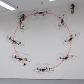
\includegraphics{graphics/QuadLoopSnapshots}
 \caption{Snapshots of the lsr-quadcopter tracking a looping trajectory}
 \label{fig:introQuadLoopSnapshots}
\end{figure}

From a mechanical point of view, these multicopters may be modelled as a free rigid body moving within Earth's gravity.
The difference between them is only the placement of the actuators:
the tricopter is fully-actuated, so it poses the easiest control task.
The quadcopter only has four actuators for its six degrees of freedom, i.e. it is underactuated.
However, its model is well known to be a configuration flat system and corresponding standard control design approaches may be applied.
The bicopter is (probably) not a flat system and consequently, poses the toughest control task.


\section{Motivation example}\label{sec:MotivationRigidBodyAttitude}
Consider a free rigid body as illustrated in the middle of \autoref{fig:ModelingIllustration}, but fixed at its center of mass, i.e.\ it may only rotate about this point.
For simplicity, we also assume that the chosen frame coincides with its principle axis and there are three independent control torques about these axis.
Then the coefficients of inertia are $\J = \diag(\Jx,\Jy,\Jz)$.

\paragraph{Lagrange's equation.}
For application of the Lagrange formalism we need to parameterize the system by minimal generalized coordinates.
A popular choice for the rigid body orientation are Euler angles in the \textit{roll-pitch-yaw} convention:
\begin{subequations}\label{eq:EulerAngleParam}
\begin{align}
 \R(\genCoord) &=
 \begin{bmatrix}
  \cyaw \cpit & -\syaw \crol+\cyaw \spit \srol & \syaw \srol+\cyaw \spit \crol \\
  \syaw \cpit & \cyaw \crol+\syaw \spit \srol & -\cyaw \srol+\syaw \spit \crol \\
  -\spit & \cpit \srol & \cpit \crol  
 \end{bmatrix},
 \label{eq:EulerAngleParamR}
\\
 \w(\genCoord, \genCoordd) &=
 \underbrace{\begin{bmatrix}
  1 & 0 & -\spit \\
  0 & \crol & \cpit \srol \\
  0 & -\srol & \cpit \crol
 \end{bmatrix}}_{\kinBasisMat(\genCoord)}
 \underbrace{\begin{bmatrix} \rold \\ \pitd \\ \yawd \end{bmatrix}}_{\genCoordd}.
 \label{eq:EulerAngleParamW}
\end{align}
\end{subequations}
The shortcut notation $\syaw := \sin(\yaw)$ and $\cyaw := \cos(\yaw)$ used here, will be used throughout this text.
With this, we may formulate the kinetic energy $\kineticEnergy(\genCoord, \genCoordd) = \tfrac{1}{2} (\w(\genCoord, \genCoordd))^\top \J \w(\genCoord, \genCoordd)$ which coincides with the Lagrangian since there is no potential energy.
% \begin{align}
%  \kineticEnergy(\genCoord, \genCoordd)
%  = \tfrac{1}{2} (\w(\genCoord, \genCoordd))^\top \J \, \w(\genCoord, \genCoordd)
%  = \tfrac{1}{2} \genCoordd^\top \underbrace{(\kinBasisMat(\genCoord))^\top \J \, \kinBasisMat(\genCoord)}_{\sysInertiaMat(\genCoord)} \genCoordd,
% \end{align}
Evaluation of Lagrange's equation \eqref{eq:LagrangeEq} yields the equations of motion 
\begin{multline}\label{eq:LagrangeEqRBAttitude}
 \underbrace{\begin{bmatrix}
  \Jx & 0 & -\Jx \spit \\
  0 & \Jy\crol^2 + \Jz\srol^2 & (\Jy-\Jz)\crol\srol\cpit \\
  -\Jx \spit & (\Jy-\Jz)\crol\srol\cpit & \Jx\spit^2 + (\Jy\srol^2 + \Jz\crol^2)\cpit^2 
 \end{bmatrix}}_{\sysInertiaMat(\genCoord)}
 \underbrace{\begin{bmatrix} \roldd \\ \pitdd \\ \yawdd \end{bmatrix}}_{\genCoorddd}
\\
 + \underbrace{\begin{bmatrix}
  (\Jy-\Jz)\crol\srol \pitd^2 + \cdots \\ %(2(\Jz-\Jy)\crol^2 - \Jx + \Jy - \Jz)\cpit \yawd \pitd + \ldots \\%(-(\cpit)^2 \srol \Jy \crol+(\cpit)^2 \crol \Jz \srol) \yawd^2 \\
  2(\Jz-\Jy)\srol\crol\pitd \rold + \cdots \\ %((2 (\Jy-\Jz)\crol^2 + \Jx - \Jy + \Jz)\cpit \yawd)\rold + \ldots \\%(-\Jy \cpit (\crol)^2 \spit+\cpit (\crol)^2 \Jz \spit-\spit \Jx \cpit+\Jy \cpit \spit) \yawd^2 \\
  (2(\Jy-\Jz)\crol^2 - \Jx - \Jy + \Jz)\cpit \pitd \rold + \cdots \\ % (2(\Jy-\Jz) \cpit^2 \crol \srol \yawd) \rold + \ldots %(-\crol \Jy \spit \srol+\srol \Jz \spit \crol) \pitd^2+(2 \Jy \cpit (\crol)^2 \spit-2 \cpit (\crol)^2 \Jz \spit+2 \spit \Jx \cpit-2 \Jy \cpit \spit) \yawd \pitd
 \end{bmatrix}}_{\sysForce(\genCoord, \genCoordd)}
% = \underbrace{\begin{bmatrix} 0 & \ArmRadius & 0 & -\ArmRadius \\ \PropTorqueFaktor\srol - \ArmRadius\crol & -\PropTorqueFaktor\srol & \PropTorqueFaktor\srol + \ArmRadius\crol & -\PropTorqueFaktor\srol \\ -\PropTorqueFaktor\crol\cpit - \ArmRadius\srol\cpit & \PropTorqueFaktor\crol\cpit - \ArmRadius\cpit & -\PropTorqueFaktor\crol\cpit - \ArmRadius\srol\cpit & \PropTorqueFaktor\crol\cpit + \ArmRadius\cpit \end{bmatrix}}_{\sysInputMat(\genCoord)}
% \underbrace{\begin{bmatrix} u_1 \\ u_2 \\ u_3 \\ u_4 \end{bmatrix}}_{\sysInput}.
 = \underbrace{\begin{bmatrix}
  1 & 0 & 0 \\
  0 & \crol & -\srol \\
  -\spit & \cpit \srol & \cpit \crol
 \end{bmatrix}}_{\kinBasisMat^\top(\genCoord)}
 \underbrace{\begin{bmatrix} \taux \\ \tauy \\ \tauz \end{bmatrix}}_{\sysInput}.
\end{multline}
The entries in $\sysForce$ are not displayed here since they would fill several lines and are actually not of relevance here.
What is crucial here is that the model has singularities at $\pit=\pm\tfrac{\pi}{2}$: $\det\sysInertiaMat = \Jx\Jy\Jz\cpit^2$ and $\det\kinBasisMat = \cpit$.
For the previous example of aerobatic motions it is should be evident that singularities of this form would be unacceptable for simulation and control design. 

%Consequently this model is neither suited for a global simulation nor for application of computed torque control.

\paragraph{Euler's rotation equations.}
For the particular example of the rigid body orientation one finds another formulation of the equations of motion directly in most textbooks on mechanics, e.g.\ \cite[p.\,143]{Arnold:MathematicalMethodsOfClassicalMechanics} or \cite[p.\,145]{Schwertassek:MultibodySystems}:
%They are commonly called \textit{Euler's rotation equations}:
\begin{subequations}\label{eq:ExampleEulerEq}
\begin{align}
 \ddt
 \underbrace{\begin{bmatrix} \Rxx & \Rxy & \Rxz \\ \Ryx & \Ryy & \Ryz \\ \Rzx & \Rzy & \Rzz \end{bmatrix}}_{\R}
 =
 \underbrace{\begin{bmatrix} \Rxx & \Rxy & \Rxz \\ \Ryx & \Ryy & \Ryz \\ \Rzx & \Rzy & \Rzz \end{bmatrix}}_{\R}
 \underbrace{\begin{bmatrix} 0 & -\wz & \wy \\ \wz & 0 & -\wx \\ -\wy & \wx & 0\end{bmatrix}}_{\wedOp{\w}},
\label{eq:ExampleEulerEqKinematics}
\\
 \underbrace{\begin{bmatrix} \Jx & 0 & 0 \\ 0 & \Jy & 0 \\ 0 & 0 & \Jz \end{bmatrix}}_{\J}
 \underbrace{\begin{bmatrix} \wxd \\ \wyd \\ \wzd \end{bmatrix}}_{\dot{\w}}
 + \underbrace{\begin{bmatrix} 0 & -\wz & \wy \\ \wz & 0 & -\wx \\ -\wy & \wx & 0\end{bmatrix}}_{\wedOp{\w}}
 \underbrace{\begin{bmatrix} \Jx & 0 & 0 \\ 0 & \Jy & 0 \\ 0 & 0 & \Jz \end{bmatrix}}_{\J}
 \underbrace{\begin{bmatrix} \wx \\ \wy \\ \wz \end{bmatrix}}_{\w}
 = 
 \underbrace{\begin{bmatrix} \taux \\ \tauy \\ \tauz \end{bmatrix}}_{\sysInput}.
 %\underbrace{\begin{bmatrix} 0 & \ArmRadius & 0 & -\ArmRadius \\ -\ArmRadius & 0 & \ArmRadius & 0 \\ -\PropTorqueFaktor & \PropTorqueFaktor & -\PropTorqueFaktor & \PropTorqueFaktor \end{bmatrix}}_{\sysInputMat}
 %\underbrace{\begin{bmatrix} u_1 \\ u_2 \\ u_3 \\ u_4 \end{bmatrix}}_{\sysInput}.
 \label{eq:ExampleEulerEqKinetics}
\end{align}
\end{subequations}
The 9 coefficients of the matrix $\R$ have to obey the constraint $\R^\top \R = \idMat[3]$.
However, it can be shown that if this is fulfilled for the initial condition $\R(t_0)$, then the kinematic equation \eqref{eq:ExampleEulerEqKinematics} ensures that the condition remains fulfilled.
This formulation has no singularities and is well suited for global simulation.
Moreover, loosely speaking, its mathematical structure reflects the physical symmetries of the model.
The obvious draw-back is that due to the lack of generalized coordinates, its unclear how a method like computed torque could be applied.

\paragraph{Discussion.}
Euler's equations \eqref{eq:ExampleEulerEq} and \eqref{eq:LagrangeEqRBAttitude} describe the same system.
In fact one may plug \eqref{eq:EulerAngleParamW} into \eqref{eq:ExampleEulerEqKinetics} and multiply it by $\kinBasisMat^\top$ to obtain \eqref{eq:LagrangeEqRBAttitude}.

Each of these formulations has its advantages and draw-backs:
Euler's equations are more compact and have a symmetric structure in contrast to \eqref{eq:LagrangeEqRBAttitude}.
The downside is that they require 9 coordinates, the coefficients of the rotation matrix $\R$, to parameterize the attitude, whereas the Euler-angles $\genCoord$ only require 3.
The crucial advantage of Lagrange's equation \eqref{eq:LagrangeEq} is, that it holds for \textit{any} finite dimensional and holonomic mechanical system, whereas Euler's equations only hold for this particular example.
However, for this example, the equations \eqref{eq:LagrangeEqRBAttitude} are quite cumbersome and lack an obvious structure.
Probably the worst fact is that the inertia matrix $\sysInertiaMat(\genCoord)$ is singular at the point $\pit=\pm\tfrac{\pi}{2}$ and consequently $\genCoorddd$ is undefined at these points.

It should be stressed that there is no physical reason for the singularity in the Lagrangian version \eqref{eq:LagrangeEqRBAttitude}, it is rather a consequence of an unsuitable parameterization of the system.
This is pointed out in \cite[sec.\ 1.1.1]{Schwertassek:MultibodySystems} as:
\textit{
[The scientists of the Eighteenth Century] recognized that there was something about rotation [\ldots] which somehow made the analysis of rotation a problem of higher order difficulty. 
We now know that the problem is in the mathematics, not the physics, but the problem is still with us.
}

The set of 3-dimensional rotation matrices $\R\in\SpecialOrthogonalGroup(3)$ captures the actual configuration space of the rigid body orientation well, but it is difficult to work with since the coefficients of the rotation matrix are not independent.
Since $\R\in\SpecialOrthogonalGroup(3)$ is compact while $\RealNum^3$ is not, there is no bijection between them, see also \cite[sec.\ 1.1d]{Frankel:GeometryOfPhysics}.
The chosen set of Euler angles may be regarded as a surjective but not injective function from $\RealNum^3$ to $\R\in\SpecialOrthogonalGroup(3)$ in a similar manner as latitude and longitude serve as coordinates for Earth's surface. 
The Euler angles are unsuited at the so called gimbal lock ($\pit=\pm 90^\circ$) just as longitude fails at Earths poles.


\section{Goal and outline of this work}
The first chapter reviews established methods of analytical mechanics with the addition of allowing redundant coordinates (like the coefficients of a rotation matrix $\R$) and nonholonomic velocity coordinates (like the coefficients of the angular velocity $\w$).
It will present a formulation that can derive both of the presented equations of motion for the motivation example, but holds for general finite-dimensional mechanical systems.

The second chapter specializes to rigid body systems, i.e. systems that consist of several interconnected rigid bodies.
It presents an algorithm that derives the equations of motion based on chosen coordinates and given constitutive parameters.
Furthermore, natural formulations of stiffness, dissipation and inertia for a rigid body are established.

The third chapter proposes tracking control algorithms for rigid body systems.
Based on the findings of the second chapter it will present three control algorithms motivated by defining desired stiffness, damping and inertia of the resulting controlled system.
Furthermore, these algorithms are extended to tackle underactuated systems.
These algorithms are discussed through several examples.

The fourth chapter presents the developed quadcopter and tricopter and their performance for real control of aerobatic maneuvers.



\chapter{Some math}\label{chap:Math}
This chapter reviews some established mathematical concepts in particular for the context of redundant coordinates.
\section{Coordinates}\label{sec:MathCoordinates}
The example of the rigid body orientation showed that, though its degree of freedom is $\dimConfigSpace=3$, it cannot be \textit{globally} parameterized by 3 coordinates without having singularities.
In other words, the configuration space of the rigid body orientation is not isomorphic to $\RealNum^3$ and is called a nonlinear manifold.

If interested in a global parameterization of a $\dimConfigSpace$ dimensional nonlinear manifold, there are two common approaches:
\begin{enumerate}
 \item Choose a finite number of overlapping local charts with with \textit{minimal} coordinates $\genCoord \in \RealNum^\dimConfigSpace$, e.g. four distinct sets of Euler angles for the rigid body attitude \cite{Grafarend:AtlasSO3}.
 As this is the common way of defining a smooth manifold, this is always possible.
 \item Choose one parameterization with \textit{redundant} coordinates $\sysCoord \in \RealNum^{\numCoord}$, i.e. coordinates that are constrained by smooth equations of the form $\geoConstraint(\sysCoord) = \tuple{0}$.
 E.g. the coefficients of the rotation matrix as done in \eqref{eq:ExampleEulerEq}.
 \textit{Whitney embedding theorem} states that this is always possible with at least $\numCoord = 2\dimConfigSpace$ coordinates.
\end{enumerate}
Both approaches have benefits and drawbacks depending on the application, but the first approach and the use of minimal coordinates is far more dominant in the literature.
This work utilizes the second approach.

%Another way for a global parameterization of nonlinear configuration manifolds is motivated from the \textit{Whitney embedding theorem} (see e.g.\ \cite[Theo.\,6.14]{Lee:SmoothManifolds}), that states: \textit{Every smooth manifold of dimension $\dimConfigSpace$ can be smoothly embedded in the Euclidean space $\RealNum^{2\dimConfigSpace}$.}
%Note that $2\dimConfigSpace$ is a worst case bound, i.e.\ for a particular example a lower dimension for the embedding space might work and a higher dimension is permitted anyway.

\subsection{Redundant configuration coordinates}\label{sec:MathConfigCoord}
In the notation of this work, we use $\numCoord > 0$ coordinates $\sysCoord(t) = [\sysCoordCoeff{1}(t),\ldots,\sysCoordCoeff{\numCoord}(t)]^\top \in \RealNum^\numCoord$ that might be constrained by $\numGeoConst \geq 0$ smooth functions of the form $\geoConstraint(\sysCoord) = [\geoConstraintCoeff{1}(\sysCoord), \ldots, \geoConstraintCoeff{\numGeoConst}(\sysCoord)]^\top = \tuple{0}$.
For $\numGeoConst > 0$ these coordinates are not independent and are commonly called \textit{redundant}.
The set of mutually admissible coordinates is called the configuration space $\configSpace$:
\begin{align}
 \configSpace = \{ \sysCoord \in \RealNum^{\numCoord} \, | \, \geoConstraint(\sysCoord) = \tuple{0} \}.
\end{align}
Assuming that the rank of $\pdiff[\geoConstraint]{\sysCoord}$ is constant, the dimension of the configuration space is
\begin{align}
 \dimConfigSpace = \dim \configSpace = \numCoord - \rank \pdiff[\geoConstraint]{\sysCoord}.
\end{align}For holonomic systems, $\dimConfigSpace$ is also called its degree of freedom.

Whitney embedding theorem (see e.g.\ \cite[Theo.\,6.14]{Lee:SmoothManifolds}) states that: \textit{Every smooth manifold of dimension $\dimConfigSpace$ can be smoothly embedded in the Euclidean space $\RealNum^{2\dimConfigSpace}$.}
The number $2\dimConfigSpace$ is a worst case bound, i.e.\ for a particular example a lower dimension for the embedding space $\RealNum^\numCoord$ might work and a higher dimension is permitted anyway.
For this work, it essentially guarantees the existence of a global parameterization by the set $\configSpace$ for any smooth manifold.


\subsection{Minimal velocity coordinates}
For the following it is crucial to note that a geometric constraint is equivalent to its derivative supplemented with a suitable initial condition
\begin{subequations}
\begin{align}
 \label{eq:GeoConstraint}
 &&
 \geoConstraintCoeff{\CidxI}(\sysCoord) &= 0
\\
 \label{eq:DiffGeoConstraint}
 &\Leftrightarrow&
 \pdiff[\geoConstraintCoeff{\CidxI}]{\sysCoordCoeff{\GidxI}}(\sysCoord) \sysCoordCoeffd{\GidxI} &= 0,&
 \geoConstraintCoeff{\CidxI}(\sysCoord_0) &= 0
\\
 &\Leftrightarrow&
 \pdiff[\geoConstraintCoeff{\CidxI}]{\sysCoordCoeff{\GidxI}}(\sysCoord) \sysCoordCoeffdd{\GidxI} + \frac{\partial^2 \geoConstraintCoeff{\CidxI}}{\partial \sysCoordCoeff{\GidxI} \partial \sysCoordCoeff{\GidxII}}(\sysCoord) \sysCoordCoeffd{\GidxII} \sysCoordCoeffd{\GidxI} &= 0,&
 \geoConstraintCoeff{\CidxI}(\sysCoord_0) &= 0, \ \pdiff[\geoConstraintCoeff{\CidxI}]{\sysCoordCoeff{\GidxI}}(\sysCoord_0) \sysCoordCoeffd{\GidxI}_0 = 0
\\
 &&
 &\ldots \nonumber
\end{align}
\end{subequations}
where $\sysCoord_0 = \sysCoord(t_0)$.
Even though \eqref{eq:GeoConstraint} might be nonlinear, its derivative \eqref{eq:DiffGeoConstraint} is always \textit{linear} in the velocities $\sysCoordd$.
So here it is reasonable to choose \textit{minimal velocity coordinates}:
Let $\kinMat(\sysCoord) \in \RealNum^{\numCoord\times\dimConfigSpace}$ be a matrix with the properties $\pdiff[\geoConstraint]{\sysCoord} \kinMat = \mat{0}$ and $\rank \kinMat = \dimConfigSpace$.
The first property of $\kinMat(\sysCoord)$ is that these columns of $\kinMat(\sysCoord)$ are orthogonal to the rows of $\pdiff[\geoConstraint]{\sysCoord}(\sysCoord)$.
The second property implies that the columns of $\kinMat(\sysCoord)$ are linearly independent.
So the columns of $\kinMat(\sysCoord)$ can be interpreted as a \textit{basis vectors} for the tangent space $\Tangent[\sysCoord] \configSpace$.
We can capture all allowed velocities $\sysCoordd(t)$ by the minimal velocity coordinates $\sysVel(t) \in \RealNum^{\dimConfigSpace}$ through
\begin{align}\label{eq:MyKinematics}
 \sysCoordd = \kinMat(\sysCoord) \sysVel
\end{align}
This kinematic relation \eqref{eq:MyKinematics} ensures that the time derivative \eqref{eq:DiffGeoConstraint} of the geometric constraint is fulfilled, and consequently the geometric constraint only has to be imposed on the initial condition $\geoConstraint(\sysCoord(t_0)) = \tuple{0}$.

% \fixme{Existence for A? guaranteed for Lie groups: the Lie algebra at the identity can be translated around the manifold by the group operation}
% 
% \fixme{Construction of $\kinMat$ by matrix inversion}

\begin{Example}
Consider a single particle constrained to a circle of radius $\rho$ as illustrated in \autoref{fig:ParticleOnCircle}.

\begin{minipage}{\textwidth}
 \centering
 \input{graphics/ParticleOnCircle.pdf_tex}
 \captionof{figure}{Particle on a circle}
 \label{fig:ParticleOnCircle}
\end{minipage}

We use the its Cartesian position $[\sysCoordCoeff{1}, \sysCoordCoeff{2}]^\top \in \RealNum^2$ constrained by $\geoConstraintCoeff{} = (\sysCoordCoeff{1})^2 + (\sysCoordCoeff{2})^2 - \rho^2 = 0$ as configuration coordinates.
A reasonable choice for the kinematics matrix $\kinMat$ is motivated from
\begin{align}
 \underbrace{\big[ 2\sysCoordCoeff{1} \ 2\sysCoordCoeff{2} \big]}_{\pdiff[\geoConstraintCoeff{}]{\sysCoord}}
 \underbrace{\begin{bmatrix} -\sysCoordCoeff{2} \\ \sysCoordCoeff{1} \end{bmatrix}}_{\kinMat}
 = 0
\end{align}
\end{Example}

\begin{Example}\label{Example:KinMatSO3}
Consider again the system from Example \fixme{Example:ThreeParticles}.
Instead of parameterizing the rotation matrix $\R$ by minimal coordinates we now take its 9 coefficients $\sysCoord = [\Rxx, \Ryx, \Rzx, \Rxy, \Ryy, \Rzy, \Rxz, \Ryz, \Rzz]^\top \in \RealNum^{9}$ as configuration coordinates.
The constraints $\R^\top \R = \idMat[3]$ and $\det\R = 1$ read
\begin{align}\label{eq:constraintSO3}
 \geoConstraint(\sysCoord) = 
  \begin{bmatrix}
  (\Rxx)^2 + (\Ryx)^2 + (\Rzx)^2 - 1 \\
  (\Rxy)^2 + (\Ryy)^2 + (\Rzy)^2 - 1 \\
  (\Rxz)^2 + (\Ryz)^2 + (\Rzz)^2 - 1 \\
  \Rxy \Rxz + \Ryy \Ryz + \Rzy \Rzz \\
  \Rxx \Rxz + \Ryx \Ryz + \Rzx \Rzz \\
  \Rxx \Rxy + \Ryx \Ryy + \Rzx \Rzy \\
  \Rxx \Ryy \Rzz + \Rxy \Ryz \Rzx + \Rxz \Ryx \Rzy - \Rxx \Ryz \Rzy - \Rxy \Ryx \Rzz - \Rxz \Ryy \Rzx - 1
 \end{bmatrix}
 = \tuple{0}.
\end{align}
The 9 conditions $\R^\top \R = \idMat[3]$ yields due to symmetry only 6 constraints and already imply $\det\R = \pm 1$.
Since the determinant is a smooth function, the corresponding manifold must consist of two disjoint components, one with $\det\R = +1$ (proper rotations) and one with $\det\R=-1$ (rotations with reflection).
So the additional constraint $\det\R = +1$ does not change the dimension of the configuration space.
Formally this means $\rank\pdiff[\geoConstraint]{\sysCoord} = 6$ and consequently $\dim\configSpace = 9-6 = 3$.
A kinematics matrix with $\pdiff[\geoConstraint]{\sysCoord} \kinMat = \mat{0}$ and $\rank\kinMat = 3$ is given by
\begin{align}\label{eq:KinMatSO3}
 \mat{A}(\sysCoord) =
 \begin{bmatrix}
  0 & -\Rxz & \Rxy \\
  0 & -\Ryz & \Ryy \\
  0 & -\Rzz & \Rzy \\
  \Rxz & 0 & -\Rxx \\
  \Ryz & 0 & -\Ryx \\
  \Rzz & 0 & -\Rzx \\
  -\Rxy & \Rxx & 0 \\
  -\Ryy & \Ryx & 0 \\
  -\Rzy & \Rzx & 0
 \end{bmatrix}.
\end{align}
The resulting kinematic equation $\sysCoordd = \kinMat(\sysCoord) \sysVel$ can be reordered to the matrix equation $\Rd = \R \wedOp(\sysVel)$ by introducing the \textit{wedge operator} defined as
\begin{align}
 \wedOp \begin{bmatrix} \sysVelCoeff{1} \\ \sysVelCoeff{2} \\ \sysVelCoeff{3} \end{bmatrix} = \begin{bmatrix} 0 & -\sysVelCoeff{3} & \sysVelCoeff{2} \\ \sysVelCoeff{3} & 0 & -\sysVelCoeff{1} \\ -\sysVelCoeff{2} & \sysVelCoeff{1} & 0 \end{bmatrix}.
\end{align}
\end{Example}

\paragraph{Pseudoinverse}
For any matrix $\mat{S}\in\RealNum^{m\times n}$ there exists a unique \textit{(Moore-Penrose) pseudoinverse} $\mat{S}^+ \in \RealNum^{n\times m}$ determined by the following conditions \cite[Theo.\ 1]{Penrose:Pseudoinverse}:
\begin{subequations}\label{eq:PenroseConditions}
\begin{align}
 \mat{S} \mat{S}^+ \mat{S} &= \mat{S},
\\
 \mat{S}^+ \mat{S} \mat{S}^+ &= \mat{S}^+,
\\
 (\mat{S} \mat{S}^+)^\top &= \mat{S} \mat{S}^+,
\\
 (\mat{S}^+ \mat{S})^\top &= \mat{S}^+ \mat{S}.
\end{align}
\end{subequations}
If the matrix $\mat{S}$ has linearly independent columns, its pseudoinverse is $\mat{S}^+ = (\mat{S}^\top \mat{S})^{-1} \mat{S}^\top$.
Similarly, if $\mat{S}$ has linearly independent rows, its pseudoinverse is $\mat{S}^+ = \mat{S}^\top (\mat{S} \mat{S}^\top)^{-1}$.
Consequently, if $\mat{S}$ is invertible (independent rows and columns) the pseudoinverse coincides with the inverse $\mat{S}^+ = \mat{S}^{-1}$.

\paragraph{Some identities involving the pseudo-inverse.}
Define $\kinBasisMat(\sysCoord) \in \RealNum^{\dimConfigSpace\times\numCoord}$ as $\kinBasisMat = \kinMat^+ = (\kinMat^\top \kinMat)^{-1} \kinMat^\top$, i.e. the pseudoinverse of the kinematics matrix $\kinMat$.
Note that this implies $\kinBasisMat \kinMat = \idMat[\dimConfigSpace]$, but $\kinMat \kinBasisMat \neq \idMat[\numCoord]$.
We also introduce the matrices $\geoConstraintMat = \pdiff[\geoConstraint]{\sysCoord}$ and $\InvGeoConstraintMat = \geoConstraintMat^+$.
With $\geoConstraintMat\kinMat = \mat{0}$ and the Penrose conditions \eqref{eq:PenroseConditions}, we can show\footnote{$\InvGeoConstraintMat^\top \kinMat = (\InvGeoConstraintMat \geoConstraintMat \InvGeoConstraintMat)^\top \kinMat = \InvGeoConstraintMat^\top (\InvGeoConstraintMat \geoConstraintMat)^\top \kinMat = \InvGeoConstraintMat^\top \InvGeoConstraintMat \geoConstraintMat \kinMat = \mat{0}$} that $\InvGeoConstraintMat^\top \kinMat = \mat{0}$ and $\kinBasisMat^\top \geoConstraintMat = \mat{0}$.
Furthermore, since $\rank\InvGeoConstraintMat = \rank\geoConstraintMat = \numCoord - \dimConfigSpace$ the columns of $\InvGeoConstraintMat(\sysCoord)$ span the complementary space $(\Tangent[\sysCoord]\configSpace)^\bot$ though they might not be a basis since the columns might not be linearly independent.

The matrix $\mat{P} = \kinMat \kinBasisMat$ is an \textit{orthogonal projector}, i.e.\ $\mat{P}^2 = \mat{P}$ and $\mat{P}^\top = \mat{P}$ which result directly from the Penrose conditions \eqref{eq:PenroseConditions}.
Since $\InvGeoConstraintMat$ spans the complementary space $(\Tangent[\sysCoord]\configSpace)^\bot$, the unique orthogonal projector from $\RealNum^\numCoord$ to $(\Tangent[\sysCoord]\configSpace)^\bot$ can be expressed as $\mat{P}^\bot = \InvGeoConstraintMat \geoConstraintMat$.
The identity $\mat{P} + \mat{P}^\bot = \idMat[\numCoord]$ implies
\begin{align}\label{eq:ProjectionIdentity}
 \kinMat \kinBasisMat + \InvGeoConstraintMat \geoConstraintMat = \idMat[\numCoord].
\end{align}

% In summary: Given a matrix $\geoConstraintMat \in \RealNum^{\numGeoConst\times\numCoord}$ and a matrix $\kinMat \in \RealNum^{\numCoord\times\dimConfigSpace}$ with full column rank and $\geoConstraintMat\kinMat = \mat{0}$ we have
% \begin{subequations}
% \begin{align}
%  \InvGeoConstraintMat &= \geoConstraintMat^+,
% \\
%  \kinBasisMat &= \kinMat^+ = (\kinMat^\top \kinMat)^{-1} \kinMat^\top
% \\
%  \kinBasisMat \kinMat &= \idMat[\dimConfigSpace]
% \\
%  \kinMat \kinBasisMat + \InvGeoConstraintMat \geoConstraintMat &= \idMat[\numCoord].
% \end{align}
% \end{subequations}

\section{Calculus}
This section reviews some of the established tools of calculus for the context of redundant coordinates and nonholonomic velocity coordinates as introduced in the previous section.

\subsection{Directional derivative and Hessian}
Consider a function $\potentialEnergy : \RealNum^{\numCoord} \rightarrow \RealNum$ and a curve $\sysCoord : \RealNum \rightarrow \configSpace$.
Since $\configSpace \subset \RealNum^{\numCoord}$, their composition $\potentialEnergy \circ \sysCoord = f : \RealNum \rightarrow \RealNum$ is a scalar function and has the the Taylor expansion
\begin{multline}
 \underbrace{\potentialEnergy(\sysCoord(t))}_{f(t)}
 = \underbrace{\potentialEnergy(\sysCoord(0))}_{f(0)}
  \, + \, t \underbrace{\pdiff[\potentialEnergy]{\sysCoordCoeff{\GidxI}}(\sysCoord(0)) \sysCoordCoeffd{\GidxI}(0)}_{\dot{f}(0)}
 \\
  + \tfrac{1}{2} t^2 \underbrace{\Big( \frac{\partial^2 \potentialEnergy}{\partial\sysCoordCoeff{\GidxII} \partial\sysCoordCoeff{\GidxI}}(\sysCoord(0)) \sysCoordCoeffd{\GidxI}(0) \sysCoordCoeffd{\GidxII}(0) + \pdiff[\potentialEnergy]{\sysCoordCoeff{\GidxI}}(\sysCoord(0)) \sysCoordCoeffdd{\GidxI}(0)\Big)}_{\ddot{f}(0)}
  + \, \mathcal{O}(t^3).
\end{multline}
Now let the curve be parameterized by $\sysCoordd(t) = \kinMat(\sysCoord(t))\sysVel(t)$ and we use the shorthand notations $\sysCoordB = \sysCoord(0)$, $\sysVelB = \sysVel(0)$ and $\kinMatB = \kinMat(\sysCoord(0))$ to write
\begin{multline}
 \potentialEnergy(\sysCoord(t))
 = \potentialEnergy(\sysCoordB)
  + t \pdiff[\potentialEnergy]{\sysCoordCoeff{\GidxI}}(\sysCoordB) \kinMatCoeffB{\GidxI}{\LidxI} \sysVelCoeffB{\LidxI}
\\
  + \tfrac{1}{2} t^2 \Big( \frac{\partial^2 \potentialEnergy}{\partial\sysCoordCoeff{\GidxII} \partial\sysCoordCoeff{\GidxI}}(\sysCoordB) \kinMatCoeffB{\GidxI}{\LidxI} \kinMatCoeffB{\GidxII}{\LidxII} \sysVelCoeffB{\LidxI} \sysVelCoeffB{\LidxII} + \pdiff[\potentialEnergy]{\sysCoordCoeff{\GidxI}}(\sysCoordB) \Big( \pdiff[\kinMatCoeff{\GidxI}{\LidxI}]{\sysCoordCoeff{\GidxII}}(\sysCoordB) \kinMatCoeffB{\GidxII}{\LidxII} \sysVelCoeffB{\LidxI}\sysVelCoeffB{\LidxII} + \kinMatCoeffB{\GidxI}{\LidxI} \sysVelCoeffBd{\LidxI}\Big) \Big)
  + \mathcal{O}(t^3)
\end{multline}
Introducing the notation
\begin{align}\label{eq:DefBasisDiff}
 \dirDiff{\LidxI} = \kinMatCoeff{\GidxI}{\LidxI} \pdiff{\sysCoordCoeff{\GidxI}}, \ \LidxI = 1,\ldots,\dimConfigSpace
\end{align}
for the derivative in the direction of the $\LidxI$-th basis vector, we can state the Taylor expansion as
\begin{align}
 \potentialEnergy(\sysCoord(t)) = \potentialEnergy(\sysCoordB)
  + t \, \dirDiff{\LidxI} \potentialEnergy(\sysCoordB) \sysVelCoeffB{\LidxI}
  + \tfrac{1}{2} t^2 \big( \dirDiff{\LidxI} \dirDiff{\LidxII} \potentialEnergy(\sysCoordB) \sysVelCoeffB{\LidxI} \sysVelCoeffB{\LidxII} + \dirDiff{\LidxI} \potentialEnergy(\sysCoordB) \sysVelCoeffBd{\LidxI} \big)
  + \mathcal{O}(t^3).
\label{eq:TaylorExpansionOne}
\end{align}
There are two more things we can derive from this equation:
\begin{itemize}
 \item 
If $\dirDiff{\LidxI} \potentialEnergy(\sysCoordB) = 0, \LidxI=1,\ldots,\dimConfigSpace$ then $\sysCoordB$ is called a \textit{critical point} of $\potentialEnergy$.
At a critical point the expansion \eqref{eq:TaylorExpansionOne} reduces to
\begin{align}
 \potentialEnergy(\sysCoord(t))
 &= \potentialEnergy(\sysCoordB)
  + \tfrac{1}{2} t^2 \underbrace{(\dirDiff{\LidxI} \dirDiff{\LidxII} \potentialEnergy)(\sysCoordB)}_{\bar{H}_{\LidxI\LidxII}} \sysVelCoeffB{\LidxI} \sysVelCoeffB{\LidxII}
  + \mathcal{O}(t^3).
\label{eq:TaylorExpansionTwo}
\end{align}
This relation holds for any sufficiently smooth curve $t\mapsto\sysCoord(t)$ through $\sysCoordB$ and consequently for any velocity vector $\sysVelB$ at the critical point.
So if the matrix $\bar{\mat{H}}$ is positive (negative) definite, then $\sysCoordB$ is a local minimum (maximum) of $\potentialEnergy$.

\item
Assume the curve $t\mapsto\sysCoord(t)$ is a \textit{geodesic}, i.e.\ $\sysVelCoeffd{\LidxI} = -\ConnCoeff{\LidxI}{\LidxII}{\LidxIII} \sysVelCoeff{\LidxII} \sysVelCoeff{\LidxIII}$ with the connection coefficients $\ConnCoeff{\LidxI}{\LidxII}{\LidxIII}$ that will be discussed later.
Plugging this into \eqref{eq:TaylorExpansionOne} we find a coordinate form of the \textit{Hessian tensor} $\differential^2 \potentialEnergy$ of the potential:
\begin{align}
 \potentialEnergy(\sysCoord(t))
 &= \potentialEnergy(\sysCoordB)
  + t (\dirDiff{\LidxI} \potentialEnergy)(\sysCoordB) \sysVelCoeffB{\LidxI}
  + \tfrac{1}{2} t^2 \underbrace{\big( \dirDiff{\LidxI} \dirDiff{\LidxII} \potentialEnergy - \ConnCoeff{\LidxIII}{\LidxI}{\LidxII} \dirDiff{\LidxIII} \potentialEnergy \big)}_{(\differential^2\potentialEnergy)_{\LidxI\LidxII}}(\sysCoordB)  \sysVelCoeffB{\LidxI} \sysVelCoeffB{\LidxII}
  + \mathcal{O}(t^3).
\end{align}
%The Hessian is a symmetric tensor, which follows from the definition of the connection coefficients \fixme{(??)}.
At a critical point $\sysCoordB$, the Hessian of the potential is independent of the connection coefficients $\ConnCoeff{\LidxI}{\LidxII}{\LidxIII}$ and consequently of the underlying metric.
There it coincides with the matrix $\bar{\mat{H}}$ defined in \eqref{eq:TaylorExpansionTwo}.
\end{itemize}


\subsection{Commutation coefficients}\label{sec:CommutationCoeff}
For a function $\potentialEnergy : \RealNum^{\numCoord} \rightarrow \RealNum$ we are used to the fact that partial derivatives commute, i.e.\ $\sfrac{\partial^2 \potentialEnergy}{\partial \sysCoordCoeff{\GidxI} \partial \sysCoordCoeff{\GidxII}} = \sfrac{\partial^2 \potentialEnergy}{\partial \sysCoordCoeff{\GidxII} \partial \sysCoordCoeff{\GidxI}}$.
Unfortunately this is (in general) not the case for a directional derivatives like $\dirDiff{\LidxI}$ defined in \eqref{eq:DefBasisDiff}.
Consequently we investigate the following commutation relation
\begin{align}\label{eq:DerivationCommCoeff1}
 \dirDiff{\LidxI} \dirDiff{\LidxII} \potentialEnergy - \dirDiff{\LidxII} \dirDiff{\LidxI} \potentialEnergy 
 &= \kinMatCoeff{\GidxI}{\LidxI} \pdiff{\sysCoordCoeff{\GidxI}} \bigg( \kinMatCoeff{\GidxII}{\LidxII} \pdiff[\potentialEnergy]{\sysCoordCoeff{\GidxII}}\bigg) - \kinMatCoeff{\GidxII}{\LidxII} \pdiff{\sysCoordCoeff{\GidxII}} \bigg(\kinMatCoeff{\GidxI}{\LidxI} \pdiff[\potentialEnergy ]{\sysCoordCoeff{\GidxI}} \bigg)
\nonumber\\
 &= \kinMatCoeff{\GidxI}{\LidxI} \pdiff[\kinMatCoeff{\GidxII}{\LidxII}]{\sysCoordCoeff{\GidxI}} \pdiff[\potentialEnergy]{\sysCoordCoeff{\GidxII}} - \kinMatCoeff{\GidxII}{\LidxII} \pdiff[\kinMatCoeff{\GidxI}{\LidxI}]{\sysCoordCoeff{\GidxII}} \pdiff[\potentialEnergy ]{\sysCoordCoeff{\GidxI}}
 + \kinMatCoeff{\GidxI}{\LidxI} \kinMatCoeff{\GidxII}{\LidxII} \underbrace{\bigg( \frac{\partial^2 \potentialEnergy}{\partial\sysCoordCoeff{\GidxI} \partial\sysCoordCoeff{\GidxII}} - \frac{\partial^2 \potentialEnergy}{\partial\sysCoordCoeff{\GidxII} \partial\sysCoordCoeff{\GidxI}}\bigg)}_{=\,0}
\nonumber\\[-2ex]
 &= \bigg(\kinMatCoeff{\GidxII}{\LidxI} \pdiff[\kinMatCoeff{\GidxI}{\LidxII}]{\sysCoordCoeff{\GidxII}} - \kinMatCoeff{\GidxII}{\LidxII} \pdiff[\kinMatCoeff{\GidxI}{\LidxI}]{\sysCoordCoeff{\GidxII}}\bigg) \pdiff[\potentialEnergy]{\sysCoordCoeff{\GidxI}}
 .
\end{align}
Now using the identity \eqref{eq:ProjectionIdentity} with $\geoConstraintMatCoeff{\CidxI}{\GidxI} = \pdiff[\geoConstraintCoeff{\CidxI}]{\sysCoordCoeff{\GidxI}}$ and $\geoConstraintMatCoeff{\CidxI}{\GidxI} \kinMatCoeff{\GidxI}{\LidxI} = 0 \, \Rightarrow \, \geoConstraintMatCoeff{\CidxI}{\GidxI} \pdiff[\kinMatCoeff{\GidxI}{\LidxI}]{\sysCoordCoeff{\GidxII}} = -\pdiff[\geoConstraintMatCoeff{\CidxI}{\GidxI}]{\sysCoordCoeff{\GidxII}} \kinMatCoeff{\GidxI}{\LidxI}$ to shape this expressions a bit further
\begin{align}\label{eq:DerivationCommCoeff2}
 \dirDiff{\LidxI} \dirDiff{\LidxII} \potentialEnergy - \dirDiff{\LidxII} \dirDiff{\LidxI} \potentialEnergy 
 &= \bigg(\kinMatCoeff{\GidxII}{\LidxI} \pdiff[\kinMatCoeff{\GidxI}{\LidxII}]{\sysCoordCoeff{\GidxII}} - \kinMatCoeff{\GidxII}{\LidxII} \pdiff[\kinMatCoeff{\GidxI}{\LidxI}]{\sysCoordCoeff{\GidxII}}\bigg) \overbrace{(\kinMatCoeff{\GidxIII}{\LidxIII} \kinBasisMatCoeff{\LidxIII}{\GidxI} + \InvGeoConstraintMatCoeff{\GidxIII}{\CidxI}\geoConstraintMatCoeff{\CidxI}{\GidxI})}^{\delta^{\GidxIII}_{\GidxI}}  \pdiff[\potentialEnergy]{\sysCoordCoeff{\GidxIII}}
\nonumber\\
 &= \bigg(\kinMatCoeff{\GidxII}{\LidxI} \pdiff[\kinMatCoeff{\GidxI}{\LidxII}]{\sysCoordCoeff{\GidxII}} - \kinMatCoeff{\GidxII}{\LidxII} \pdiff[\kinMatCoeff{\GidxI}{\LidxI}]{\sysCoordCoeff{\GidxII}}\bigg) \kinBasisMatCoeff{\LidxIII}{\GidxI} \kinMatCoeff{\GidxIII}{\LidxIII} \pdiff[\potentialEnergy]{\sysCoordCoeff{\GidxIII}}
 - \bigg(\kinMatCoeff{\GidxII}{\LidxI} \kinMatCoeff{\GidxI}{\LidxII} \pdiff[\geoConstraintMatCoeff{\CidxI}{\GidxI}]{\sysCoordCoeff{\GidxII}} - \kinMatCoeff{\GidxII}{\LidxII} \kinMatCoeff{\GidxI}{\LidxI} \pdiff[\geoConstraintMatCoeff{\CidxI}{\GidxI}]{\sysCoordCoeff{\GidxII}} \bigg) \InvGeoConstraintMatCoeff{\GidxIII}{\CidxI} \pdiff[\potentialEnergy]{\sysCoordCoeff{\GidxIII}}
\nonumber\\
 &= \underbrace{\bigg(\kinMatCoeff{\GidxII}{\LidxI} \pdiff[\kinMatCoeff{\GidxI}{\LidxII}]{\sysCoordCoeff{\GidxII}} - \kinMatCoeff{\GidxII}{\LidxII} \pdiff[\kinMatCoeff{\GidxI}{\LidxI}]{\sysCoordCoeff{\GidxII}}\bigg) \kinBasisMatCoeff{\LidxIII}{\GidxI}}_{\BoltzSym{\LidxIII}{\LidxI}{\LidxII}} \underbrace{\kinMatCoeff{\GidxIII}{\LidxIII} \pdiff[\potentialEnergy]{\sysCoordCoeff{\GidxIII}}}_{\dirDiff{\LidxIII} \potentialEnergy}
 - \kinMatCoeff{\GidxII}{\LidxII} \kinMatCoeff{\GidxI}{\LidxI} \underbrace{\bigg(\frac{\partial^2\geoConstraintCoeff{\CidxI}}{\partial\sysCoordCoeff{\GidxI}\partial\sysCoordCoeff{\GidxII}} - \frac{\partial^2\geoConstraintCoeff{\CidxI}}{\partial\sysCoordCoeff{\GidxII}\partial\sysCoordCoeff{\GidxI}} \bigg)}_{=\,0} \InvGeoConstraintMatCoeff{\GidxIII}{\CidxI} \pdiff[\potentialEnergy]{\sysCoordCoeff{\GidxIII}}
 .
\end{align}
Since this relation holds for any function $\potentialEnergy$ we can state it in operator form and introduce the \textit{commutation coefficients} $\BoltzSym{\LidxIII}{\LidxI}{\LidxII}$ as
\begin{align}\label{eq:DefCommutationCoeff}
 \dirDiff{\LidxI} \dirDiff{\LidxII} - \dirDiff{\LidxII} \dirDiff{\LidxI} = \BoltzSym{\LidxIII}{\LidxI}{\LidxII} \dirDiff{\LidxIII},
\qquad
 \BoltzSym{\LidxIII}{\LidxI}{\LidxII} = \big(\dirDiff{\LidxI} \kinMatCoeff{\GidxI}{\LidxII} - \dirDiff{\LidxII} \kinMatCoeff{\GidxI}{\LidxI} \big) ({\kinMatCoeff{}{}}^+)^{\LidxIII}_{\GidxI}.
\end{align}
Note the skew symmetry $\BoltzSym{\LidxIII}{\LidxI}{\LidxII} = -\BoltzSym{\LidxIII}{\LidxII}{\LidxI}$.

\begin{Example}%\label{ex:BoltzmannSymSattelite}
The commutation coefficients $\BoltzSym{\LidxIII}{\LidxI}{\LidxII}$ associated with the kinematics matrix $\kinMat$ from \eqref{eq:KinMatSO3} are
\begin{align*}
 \BoltzSym{1}{2}{3} = \BoltzSym{2}{3}{1} = \BoltzSym{3}{1}{2} &= +1,
\\
 \BoltzSym{1}{3}{2} = \BoltzSym{2}{1}{3} = \BoltzSym{3}{2}{1} &= -1,
\\
 \BoltzSym{1}{1}{1} = \BoltzSym{1}{1}{2} = \BoltzSym{1}{1}{3} = \BoltzSym{1}{2}{1} = \BoltzSym{1}{2}{2} = \BoltzSym{1}{3}{1} = \BoltzSym{1}{3}{3} &= 0,
\\
 \BoltzSym{2}{1}{1} = \BoltzSym{2}{1}{2} = \BoltzSym{2}{2}{1} = \BoltzSym{2}{2}{2} = \BoltzSym{2}{2}{3} = \BoltzSym{2}{3}{2} = \BoltzSym{2}{3}{3} &= 0,
\\
 \BoltzSym{3}{1}{1} = \BoltzSym{3}{1}{3} = \BoltzSym{3}{2}{2} = \BoltzSym{3}{2}{3} = \BoltzSym{3}{3}{1} = \BoltzSym{3}{3}{2} = \BoltzSym{3}{3}{3} &= 0.
\end{align*}
This coincides with the three dimensional Levi-Civita symbol commonly defined as
\begin{align}\label{eq:BoltzmannSymSattelite}
 \BoltzSym{\LidxIII}{\LidxI}{\LidxII} =
 \left\{
 \begin{array}{rl}
  +1, & (\LidxI,\LidxII,\LidxIII) \ \text{even permutation of} \ (1,2,3) \\
  -1, & (\LidxI,\LidxII,\LidxIII) \ \text{odd permutation of} \ (1,2,3) \\
  0, & \text{else}
 \end{array}
 \right.
 .
\end{align}
It is related to the 3 dimensional \textit{cross product} by $\tuple{a}, \tuple{b} \in \RealNum^3 \, : \, [\BoltzSym{\LidxIII}{\LidxI}{\LidxII} a^{\LidxI} b^{\LidxII}]_{\LidxIII=1..3} = \tuple{a} \times \tuple{b}$ and to the previously defined $\wedOp$ operator by $\tuple{a} \in \RealNum^3 \, : \, [\BoltzSym{\LidxIII}{\LidxI}{\LidxII} a^{\LidxI}]_{\LidxII,\LidxIII=1..3} = \wedOp(\tuple{a})$.
\end{Example}

The right hand side of \eqref{eq:DefCommutationCoeff} appears in the context of Lagrange's equation in \cite[p.\ 687]{Boltzmann:NonholCoord} and \cite[p.\ 10]{Hamel:LagrangeEuler} for the case of minimal configuration coordinates and consequently with a square matrix $\kinMat$.
In the contemporary literature on this context, the quantities $\BoltzSym{\LidxIII}{\LidxI}{\LidxII}$ are sometimes called the \textit{Boltzmann three-index symbols} \cite[sec.\,1.8]{Lurie:AnalyticalMechanics} or \textit{Hamel coefficients} \cite[p.\,75]{Bremer:ElasticMultibodyDynamics}.
The left hand side of \eqref{eq:DefCommutationCoeff} appears in the context of tensor algebra in \cite[Box 8.4]{Misner:Gravitation} where $\BoltzSym{\LidxIII}{\LidxI}{\LidxII}$ are called the \textit{commutation coefficients}.
From the way $\BoltzSym{\LidxIII}{\LidxI}{\LidxII}$ is defined here, this naming seems most fitting and will be used throughout this work. 

The case of redundant configuration coordinates and consequently a non-square matrix $\kinMat$ as derived above, is not established in the literature to the best of the authors knowledge.

It is worth noting that the commutation coefficients are \textit{invariant} to the choice of configuration coordinates $\sysCoord$, even though the coordinates appear explicitly in the definition:
For a change of configuration coordinates $\sysCoord = f(\sysCoordW)$ the commutation symbols transform like $\BoltzSymW{\LidxIII}{\LidxI}{\LidxII}(\sysCoordW) = \BoltzSym{\LidxIII}{\LidxI}{\LidxII}(f(\sysCoordW))$.
This might be obvious from a geometric point of view, but the explicit calculation of the coordinate transformation is shown in see \fixme{[sec:TrafoRules]}.
It will even turn out that for most of our examples the coefficients will be constants.

The commutation coefficients $\BoltzSym{\LidxI}{\LidxII}{\LidxIII}$ vanish if the corresponding velocity coordinates $\sysVelCoeff{\LidxI}$ are \textit{integrable}, i.e.\
\begin{align}
 \exists \ \pi^\LidxI \, : \, \dot{\pi}^\LidxI &= \sysVelCoeff{\LidxI} = \kinBasisMatCoeff{\LidxI}{\GidxI} \sysCoordCoeffd{\GidxI}&
 &\Rightarrow&
  \kinBasisMatCoeff{\LidxI}{\GidxI} &= \pdiff[\pi^i]{\sysCoordCoeff{\GidxII}}
\nonumber\\
&&
&\Rightarrow&
 \pdiff[\kinBasisMatCoeff{\LidxI}{\GidxI}]{\sysCoordCoeff{\GidxI}}
 &= \frac{\partial^2 \pi^i}{\partial \sysCoordCoeff{\GidxII} \partial \sysCoordCoeff{\GidxI}}
 = \pdiff[\kinBasisMatCoeff{\LidxI}{\beta}]{\sysCoordCoeff{\GidxI}},&
&\Rightarrow&
 \BoltzSym{\LidxI}{\LidxII}{\LidxIII} &= 0.
\end{align}
This is not the case in general.
Nevertheless the quantities $\pi$ are introduced as \textit{nonholonomic coordinates} in \cite{Boltzmann:NonholCoord} or as \textit{quasi coordinates} in \cite[sec.\,1.5]{Lurie:AnalyticalMechanics}.
Then we could write $\partial_\LidxI (\partial_\LidxII f) - \partial_\LidxII (\partial_\LidxI f) = \sfrac{\partial^2 f}{\partial \pi^\LidxI \partial \pi^\LidxII} - \sfrac{\partial^2 f}{\partial \pi^\LidxII \partial \pi^\LidxI} \neq 0$ what might lead to the conception that partial derivatives do not commute.
The commutativity clearly holds, the issue is rather $\pi$ are no proper coordinates.
To avoid confusion of this kind we do not pick up this notation here.
See also \cite{Hamel:virtuelleVerschiebungen} for an extensive discussion on this topic.


\subsection{Linearization about a trajectory}\label{sec:LinAboutTraj}
Let $\sysCoordB : [t_1, t_2] \rightarrow \configSpace$ be a smooth curve with the velocity coordinates $\sysVelB : [t_1, t_2] \rightarrow \RealNum^{\dimConfigSpace} : t \mapsto \kinMat^+(\sysCoordB(t)) \sysCoordBd(t)$.
For a small deviation $\sysCoord \approx \sysCoordB$ with $\sysCoord \in \configSpace$ we may approximate the geometric constraint as
\begin{align}
 \geoConstraint(\sysCoord) \approx \underbrace{\geoConstraint(\sysCoordB)}_{=\,\tuple{0}} + \pdiff[\geoConstraint]{\sysCoord}(\sysCoordB) (\sysCoord - \sysCoordB) = \tuple{0}.
\end{align}
Since this constraint is affine w.r.t.\ $\sysCoord$ it is reasonable to use a the basis $\LinErrorCoord(t) \in \RealNum^{\dimConfigSpace}$ for the deviated configuration coordinates:
\begin{align}
 \sysCoord = \sysCoordB + \kinMat(\sysCoordB) \LinErrorCoord,
\qquad
 \LinErrorCoord = \kinMat^+(\sysCoordB) (\sysCoord - \sysCoordB),
\end{align}
For the velocity coordinates $\sysVel$ of the deviated curve $\sysCoord$ we use again the first order approximation and $\kinBasisMat = \kinMat^+$:
\begin{align}
 \sysVelCoeff{\LidxI} &= \kinBasisMatCoeff{\LidxI}{\GidxI}(\sysCoord) \sysCoordCoeffd{\GidxI}
\nonumber\\
 &\approx \kinBasisMatCoeff{\LidxI}{\GidxI}(\sysCoordB + \kinMat(\sysCoordB) \LinErrorCoord) \tdiff{t} \big( \sysCoordCoeffB{\GidxI} + \kinMatCoeff{\GidxI}{\LidxII}(\sysCoordB) \, \LinErrorCoordCoeff{\LidxII} \big)
% \big( \sysCoordCoeffBd{\GidxI} + \tpdiff[\kinMatCoeff{\GidxI}{\LidxII}]{\sysCoordCoeff{\GidxII}}(\sysCoordB) \, \sysCoordCoeffRd{\GidxII} \LinErrorCoordCoeff{\LidxII} + \kinMatCoeff{\GidxI}{\LidxII}(\sysCoordB) \, \LinErrorCoordCoeffd{\LidxII} \big)
\nonumber\\
 &\approx \kinBasisMatCoeff{\LidxI}{\GidxI}(\sysCoordB) \big( \sysCoordCoeffRd{\GidxI} + \tpdiff[\kinMatCoeff{\GidxI}{\LidxII}]{\sysCoordCoeff{\GidxII}}(\sysCoordB) \, \sysCoordCoeffRd{\GidxII} \LinErrorCoordCoeff{\LidxII} + \kinMatCoeff{\GidxI}{\LidxII}(\sysCoordB) \, \LinErrorCoordCoeffd{\LidxII} \big)
  + \tpdiff[\kinBasisMatCoeff{\LidxI}{\GidxI}]{\sysCoordCoeff{\GidxII}}(\sysCoordB)  \kinMatCoeff{\GidxII}{\LidxII}(\sysCoordB) \, \LinErrorCoordCoeff{\LidxII} \sysCoordCoeffRd{\GidxI}
\nonumber\\
%  &= \underbrace{\kinBasisMatCoeff{\LidxI}{\GidxI}(\sysCoordB) \sysCoordCoeffRd{\GidxI}}_{\sysVelCoeffB{\LidxI}}
%   + \underbrace{\kinBasisMatCoeff{\LidxI}{\GidxI}(\sysCoordB) \kinMatCoeff{\GidxI}{\LidxII}(\sysCoordB)}_{\delta^\LidxI_\LidxII} \LinErrorCoordCoeffd{\LidxII}
%   + \underbrace{\big( \tpdiff[\kinBasisMatCoeff{\LidxI}{\GidxI}]{\sysCoordCoeff{\GidxII}}(\sysCoordB) - \tpdiff[\kinBasisMatCoeff{\LidxI}{\GidxII}]{\sysCoordCoeff{\GidxI}}(\sysCoordB) \big) \kinMatCoeff{\GidxII}{\LidxII}(\sysCoordB)  \kinMatCoeff{\GidxI}{\LidxIII}(\sysCoordB)}_{\BoltzSym{\LidxI}{\LidxIII}{\LidxII}(\sysCoordB)} \sysVelCoeffB{\LidxIII} \LinErrorCoordCoeff{\LidxII}
% \nonumber\\
 &= \sysVelCoeffB{\LidxI} + \LinErrorCoordCoeffd{\LidxI} + \BoltzSym{\LidxI}{\LidxIII}{\LidxII}(\sysCoordB) \sysVelCoeffB{\LidxIII} \LinErrorCoordCoeff{\LidxII}
\end{align}
Using these results we may formulate an approximation of a general smooth function $f$ along the trajectory $t \mapsto \sysCoordB(t)$ as 
\begin{align}
 f(\sysCoord, \sysVel, \sysVeld) 
  &\approx f(\sysCoordB, \sysVelB, \sysVelBd) 
  + \pdiff[f]{\sysCoordCoeff{\GidxI}}(\sysCoordB, \sysVelB, \sysVelBd) (\sysCoordCoeff{\GidxI} - \sysCoordCoeffB{\GidxI})
  + \pdiff[f]{\sysVelCoeff{\LidxI}}(\sysCoordB, \sysVelB, \sysVelBd) (\sysVelCoeff{\LidxI} - \sysVelCoeffB{\LidxI})
\nonumber\\
  &\qquad + \pdiff[f]{\sysVelCoeffd{\LidxI}}(\sysCoordB, \sysVelB, \sysVelBd) (\sysVelCoeffd{\LidxI} - \sysVelCoeffBd{\LidxI})
\nonumber\\
  &\approx f(\sysCoordB, \sysVelB, \sysVelBd) 
  + (\dirDiff{\LidxI}f) (\sysCoordB, \sysVelB, \sysVelBd) \LinErrorCoordCoeff{\LidxI}
  + \pdiff[f]{\sysVelCoeff{\LidxI}}(\sysCoordB, \sysVelB, \sysVelBd) (\LinErrorCoordCoeffd{\LidxI} + \BoltzSym{\LidxI}{\LidxIII}{\LidxII}(\sysCoordB) \sysVelCoeffB{\LidxIII} \LinErrorCoordCoeff{\LidxII})
\nonumber\\
  &\qquad 
  + \pdiff[f]{\sysVelCoeffd{\LidxI}}(\sysCoordB, \sysVelB, \sysVelBd) (\LinErrorCoordCoeffdd{\LidxI} + \BoltzSym{\LidxI}{\LidxIII}{\LidxII}(\sysCoordB) \sysVelCoeffB{\LidxIII} \LinErrorCoordCoeffd{\LidxII}  + \BoltzSym{\LidxI}{\LidxIII}{\LidxII}(\sysCoordB) \sysVelCoeffBd{\LidxIII} \LinErrorCoordCoeff{\LidxII}  + \dirDiff{\LidxIV}\BoltzSym{\LidxI}{\LidxIII}{\LidxII}(\sysCoordB) \sysVelCoeffB{\LidxIV} \sysVelCoeffB{\LidxIII} \LinErrorCoordCoeff{\LidxII})
\nonumber\\
 &= \bar{f} + \bar{F}^0_\LidxI \LinErrorCoordCoeff{\LidxI} + \bar{F}^1_\LidxI \LinErrorCoordCoeffd{\LidxI} + \bar{F}^2_\LidxI \LinErrorCoordCoeffdd{\LidxI}
\end{align}
where
\begin{align*}
 \bar{f} &= f(\sysCoordB, \sysVelB, \sysVelBd),
\\
 \bar{F}^0_\LidxI &= (\dirDiff{\LidxI}f) (\sysCoordB, \sysVelB, \sysVelBd) + \pdiff[f]{\sysVelCoeff{\LidxII}}(\sysCoordB, \sysVelB, \sysVelBd) \BoltzSym{\LidxII}{\LidxIII}{\LidxI}(\sysCoordB) \sysVelCoeffB{\LidxIII} + \pdiff[f]{\sysVelCoeffd{\LidxII}}(\sysCoordB, \sysVelB, \sysVelBd) \big( \BoltzSym{\LidxII}{\LidxIII}{\LidxI}(\sysCoordB) \sysVelCoeffBd{\LidxIII} + \dirDiff{\LidxIV}\BoltzSym{\LidxII}{\LidxIII}{\LidxI}(\sysCoordB) \sysVelCoeffB{\LidxIV} \sysVelCoeffB{\LidxIII} \big),
\\
 \bar{F}^1_\LidxI &= \pdiff[f]{\sysVelCoeff{\LidxI}}(\sysCoordB, \sysVelB, \sysVelBd) + \pdiff[f]{\sysVelCoeffd{\LidxII}}(\sysCoordB, \sysVelB, \sysVelBd) \BoltzSym{\LidxII}{\LidxIII}{\LidxI}(\sysCoordB) \sysVelCoeffB{\LidxIII},
\\
 \bar{F}^2_\LidxI &= \pdiff[f]{\sysVelCoeffd{\LidxI}}(\sysCoordB, \sysVelB, \sysVelBd).
\end{align*}
Evidently, the expressions simplify significantly is the velocity coordinates are holonomic, i.e. $\BoltzSym{}{}{} = 0$, or if the approximation is about a static point $\sysCoordB = \const \Rightarrow \sysVel = \tuple{0}$.


\subsection{Calculus of variations}\label{sec:CalculusOfVariations}
The calculus of variations is concerned with the extremals of functionals, i.e. functions of functions. %\cite[sec.\,12]{Arnold:MathematicalMethodsOfClassicalMechanics}.
For the particular context of classical mechanics we are interested in the curves $t \mapsto \sysCoord(t)$ for which the functional
\begin{align}\label{eq:Functional}
 \mathcal{J}[\sysCoord] = \int_{t_1}^{t_2} \Lagrangian(\sysCoord(t), \sysVel(t), t) \, \d t
% \tag{$\bigstar$}
\end{align}
for given boundary conditions $\sysCoord(t_1)$ and $\sysCoord(t_2)$ is \textit{stationary}.
The \textit{Lagrangian} $\Lagrangian$ is here a function of the configuration coordinates $\sysCoord$, its derivatives $\sysCoordd = \kinMat \sysVel$ parameterized in the velocity coordinates $\sysVel$ and may depend explicitly on the time $t$ as well.

For the standard case, $\sysCoord = \genCoord$ and $\sysVel = \genCoordd$, a derivation of may be found in e.g. \cite[chap.\,4, §3]{CourantHilbert1}, \cite[ch.\,II]{Lanczos:Variational} or \cite[sec.\,12]{Arnold:MathematicalMethodsOfClassicalMechanics}.
For the present case we modify the well known derivation slightly:
Suppose that $\sysCoord : [t_1, t_2] \mapsto \configSpace$ is the solution to the variational problem.
With the function $\varFkt(t) \in \RealNum^{\numCoord}$ and the parameter $\varParam\in\RealNum$ we define a perturbation to it by
\begin{align}
 \sysCoordB = \sysCoord + \varParam\varFkt.
\end{align}
We need $\sysCoordB(t) \in \configSpace$ and consequently $\geoConstraint(\sysCoordB)=\tuple{0}$.
Assuming $\varParam$ to be sufficiently small, we may use the first order approximation analog to \autoref{sec:LinAboutTraj}:
With the \textit{variation coordinates} $\varCoord : [t_1,t_2] \rightarrow \RealNum^{\dimConfigSpace}$ we parameterize $\varFkt = \kinMat(\sysCoord)\varCoord$.
Using the inverse kinematic relation $\sysVel = \kinBasisMat(\sysCoord)\sysCoordd$ we can write the functional for the varied path as
\begin{align}
 \mathcal{J}[\sysCoordB] = \int_{t_1}^{t_2} \Lagrangian\big(\sysCoord + \varParam\kinMat(\sysCoord)\varCoord, \kinBasisMat(\sysCoord + \varParam\kinMat(\sysCoord)\varCoord) \tdiff{t}(\sysCoord + \varParam\kinMat(\sysCoord)\varCoord), t\big) \, \d t =: \mathcal{P}(\varParam)
\end{align}
Now if $\sysCoord(t)$ is indeed the solution to the variational problem, then $\mathcal{P}(\varParam)$ must have a minimum at $\mathcal{P}(0)$ and consequently $\spdiff[\mathcal{P}]{\varParam}(0) = 0$.
Evaluation of this ``ordinary'' differentiation yields
\begin{align}
 0 = \pdiff[\mathcal{P}]{\varParam} \Big|_{\varParam=0} &= \int_{t_1}^{t_2} \bigg( \pdiff[\Lagrangian]{\sysCoordCoeff{\GidxI}} \kinMatCoeff{\GidxI}{\LidxI} \varCoordCoeff{\LidxI} + \pdiff[\Lagrangian]{\sysVelCoeff{\LidxI}} \bigg( \pdiff[\kinBasisMatCoeff{\LidxI}{\GidxI}]{\sysCoordCoeff{\GidxII}} \kinMatCoeff{\GidxII}{\LidxII} \varCoordCoeff{\LidxII} \sysCoordCoeffd{\GidxI} + \kinBasisMatCoeff{\LidxI}{\GidxI} \pdiff[\kinMatCoeff{\GidxI}{\LidxII}]{\sysCoordCoeff{\GidxII}} \varCoordCoeff{\LidxII} \sysCoordCoeffd{\GidxII} + \varCoordCoeffd{\LidxI}\bigg) \bigg) \, \d t
\nonumber\\
 &= \int_{t_1}^{t_2} \bigg( \dirDiff{\LidxI}\Lagrangian \, \varCoordCoeff{\LidxI} + \pdiff[\Lagrangian]{\sysVelCoeff{\LidxI}} \big( \BoltzSym{\LidxI}{\LidxIII}{\LidxII} \varCoordCoeff{\LidxII} \sysVelCoeff{\LidxIII} + \varCoordCoeffd{\LidxI} \big) \bigg) \, \d t
\end{align}
where we have found again the commutation coefficients $\BoltzSym{\LidxI}{\LidxIII}{\LidxII}$ previously derived in \eqref{eq:DefCommutationCoeff}.
% By the definition of the variation above, it is clear that it commutes with differentiation and integration, frequently quoted as $\delta \d = \d \delta$.
% Furthermore we get the relation
% \begin{align}
%  &&
%  \delta \sysCoordCoeffd{\GidxI} &= \tdiff{t} \delta \sysCoordCoeff{\GidxI}&
% \nonumber\\
%  &\Leftrightarrow&
%  \delta \kinMatCoeff{\GidxI}{\LidxI} \sysVelCoeff{\LidxI} + \kinMatCoeff{\GidxI}{\LidxI} \delta\sysVelCoeff{\LidxI} &= \kinMatCoeffd{\GidxI}{\LidxI} \varCoordCoeff{\LidxI} + \kinMatCoeff{\GidxI}{\LidxI} \varCoordCoeffd{\LidxI}
% % \nonumber\\
% %  &\Leftrightarrow&
% %  \dirDiff{\LidxII} \kinMatCoeff{\GidxI}{\LidxI} \varCoordCoeff{\LidxII} \sysVelCoeff{\LidxI} + \kinMatCoeff{\GidxI}{\LidxI} \delta\sysVelCoeff{\LidxI} &= \dirDiff{\LidxII} \kinMatCoeff{\GidxI}{\LidxI} \sysVelCoeff{\LidxII} \varCoordCoeff{\LidxI} + \kinMatCoeff{\GidxI}{\LidxI} \varCoordCoeffd{\LidxI}&
% % \GidxI &= 1,\ldots,\numCoord
% \nonumber\\
%  &\Leftrightarrow&
%  \kinMatCoeff{\GidxI}{\LidxI} \big( \delta\sysVelCoeff{\LidxI} - \varCoordCoeffd{\LidxI} \big) &= \big( \dirDiff{\LidxI} \kinMatCoeff{\GidxI}{\LidxII} - \dirDiff{\LidxII} \kinMatCoeff{\GidxI}{\LidxI} \big) \varCoordCoeff{\LidxII} \sysVelCoeff{\LidxI},&
%  \GidxI &= 1,\ldots,\numCoord
% \nonumber\\
%  &\Leftrightarrow&
%  \delta\sysVelCoeff{\LidxIII} - \varCoordCoeffd{\LidxIII} &= \underbrace{({\kinMatCoeff{}{}}^+)^{\LidxIII}_{\GidxI} \big( \dirDiff{\LidxI} \kinMatCoeff{\GidxI}{\LidxII} - \dirDiff{\LidxII} \kinMatCoeff{\GidxI}{\LidxI} \big)}_{\BoltzSym{\LidxIII}{\LidxI}{\LidxII}} \varCoordCoeff{\LidxII} \sysVelCoeff{\LidxI},&
%  \LidxI &= 1,\ldots,\dimConfigSpace
% \end{align}
% where we found again the \textit{commutation coefficients} $\BoltzSym{\LidxIII}{\LidxI}{\LidxII}$, previously derived in \eqref{eq:DefCommutationCoeff}.
Integrating by parts with the boundary conditions $\varCoord(t_1) = \varCoord(t_2) = \tuple{0}$ gives
\begin{align}
 \int_{t_1}^{t_2} \varCoordCoeff{\LidxI} \left( \kinMatCoeff{\GidxI}{\LidxI} \pdiff[\Lagrangian]{\sysCoordCoeff{\GidxI}} - \diff{t} \pdiff[\Lagrangian]{\sysVelCoeff{\LidxI}} - \BoltzSym{\LidxIII}{\LidxI}{\LidxII} \sysVelCoeff{\LidxII} \pdiff[\Lagrangian]{\sysVelCoeff{\LidxIII}} \right) \, \d t = 0.
\end{align}
Since the variation coordinates $\varCoordCoeff{\LidxI}, i=1,\ldots,\dimConfigSpace$ are independent by definition, the \textit{fundamental lemma of the calculus of variations} (see e.g.\ \cite[p.\,166]{CourantHilbert1} or \cite[p.\,57]{Arnold:MathematicalMethodsOfClassicalMechanics}) states that, for the integral to vanish, the terms in the brackets have to vanish.
Together with the kinematic equation, we have the following necessary conditions for the functional \eqref{eq:Functional} to be stationary:
\begin{subequations}\label{eq:MyEulerLagrange}
\begin{align}
 \sysCoordCoeffd{\GidxI} = \kinMatCoeff{\GidxI}{\LidxI} \sysVelCoeff{\LidxI}, \qquad
 \GidxI &= 1\ldots\numCoord,
\\
 \diff{t} \pdiff[\Lagrangian]{\sysVelCoeff{\LidxI}} + \BoltzSym{\LidxIII}{\LidxI}{\LidxII} \sysVelCoeff{\LidxII} \pdiff[\Lagrangian]{\sysVelCoeff{\LidxIII}} - \dirDiff{\LidxI}\Lagrangian = 0, \qquad
 \LidxI &= 1,\ldots,\dimConfigSpace.
\end{align}
\end{subequations}
%This, combined with the kinematic relation $\sysCoordCoeffd{\GidxI} = \kinMatCoeff{\GidxI}{\LidxI} \sysVelCoeff{\LidxI}, \GidxI=1\ldots\numCoord$, is the necessary condition for the functional \eqref{eq:Functional} to be stationary.

For the special case $\sysCoord(t)=\genCoord(t)\in\RealNum^\dimConfigSpace$ and $\sysVel(t)=\genCoordd(t)$ we have $\kinMat=\idMat[\dimConfigSpace]$ and $\BoltzSym{}{}{}=0$.
Then \eqref{eq:MyEulerLagrange} coincides with the \textit{Euler-Lagrange equation} \eqref{eq:LagrangeEq}.

\begin{Example}
Consider again the configuration coordinates $\sysCoord = [\Rx^\top, \Ry^\top, \Rz^\top]^\top$ and the velocity coordinates $\sysVel = \w$ related by $\Rd = \R \wedOp(\w)$ as discussed in the previous example \eqref{eq:KinMatSO3}.
The commutation coefficients were derived in \eqref{eq:BoltzmannSymSattelite}.

For the Lagrangian 
\begin{align}
\Lagrangian = \tfrac{1}{2} \w^\top \bodyMOI{}{} \w 
 %+ \tr(\bodyMOSp{}{}(\idMat[3]-\R)) 
\end{align}
we obain
\begin{align}
 \Big[ \diff{t} \pdiff[\Lagrangian]{\sysVelCoeff{\LidxI}} + \BoltzSym{\LidxIII}{\LidxI}{\LidxII} \sysVelCoeff{\LidxII} \pdiff[\Lagrangian]{\sysVelCoeff{\LidxIII}} - \kinMatCoeff{\GidxI}{\LidxI} \pdiff[\Lagrangian]{\sysCoordCoeff{\GidxI}} \Big]_{\LidxI=1,2,3}
 = \bodyMOI{}{} \wdot + \w \times \bodyMOI{}{} \w
 %+ \veeTwoOp(\bodyMOSp{}{} \R)
 .
\end{align}
\end{Example}


\subsection{Hamilton's equations}\label{sec:HamiltonsEquations}
\paragraph{Legendre transformation.}
Define the \textit{generalized momentum} $\genMomentum$ as
\begin{align}\label{eq:Legendre11}
 \genMomentumCoeff{\LidxI} &= \pdiff[\Lagrangian]{\sysVelCoeff{\LidxI}}, \quad \LidxI = 1,\ldots,\dimConfigSpace
% \Hamiltonian(\sysCoord, \sysVel, t) &= \genMomentumCoeff{\LidxI} \sysVelCoeff{\LidxI} - \Lagrangian(\sysCoord, \sysVel, t) = \Hamiltonian(\sysCoord, \genMomentum, t)
% \Hamiltonian &= \genMomentumCoeff{\LidxI} \sysVelCoeff{\LidxI} - \Lagrangian
 .
\end{align}
and assume that these relations can be inverted to express the velocity $\sysVel = \tuple{\zeta}(\sysCoord, \genMomentum, t)$ in terms of the momentum.
Then define the \textit{Hamiltonian} $\Hamiltonian$ as
\begin{align}\label{eq:Legendre12}
 \Hamiltonian(\sysCoord, \genMomentum, t) 
 = \Big[ \genMomentumCoeff{\LidxI} \sysVelCoeff{\LidxI} - \Lagrangian(\sysCoord, \sysVel, t) \Big]_{\sysVel = \tuple{\zeta}(\sysCoord, \genMomentum, t)}
 = \genMomentumCoeff{\LidxI} \zeta^{\LidxI}(\sysCoord, \genMomentum, t) - \Lagrangian(\sysCoord, \tuple{\zeta}(\sysCoord, \genMomentum, t), t)
 .
\end{align}
The definitions \eqref{eq:Legendre11} and \eqref{eq:Legendre12} describe the \textit{Legendre transformation} $(\Lagrangian, \sysVel) \rightarrow (\Hamiltonian, \genMomentum)$, see \cite[ch.\,VI.1]{Lanczos:Variational} or \cite[sec.\,14]{Arnold:MathematicalMethodsOfClassicalMechanics} for some geometric background.
Note that the configuration coordinates $\sysCoord$ and the time $t$ do not participate in the transformation.

\paragraph{Hamilton's canonical equations.}
Evaluation of the differentials of \eqref{eq:Legendre12}, we get the relations
\begin{subequations}\label{eq:Legendre2}
\begin{align}
 \partial_{\LidxII} \Hamiltonian &= \genMomentumCoeff{\LidxI} \partial_{\LidxII}\zeta^{\LidxI} - \partial_{\LidxII} \Lagrangian - \pdiff[\Lagrangian]{\sysVelCoeff{\LidxI}} \partial_{\LidxII}\zeta^{\LidxI}
 =  -\partial_{\LidxII} \Lagrangian
\\
 \pdiff[\Hamiltonian]{\genMomentumCoeff{\LidxII}} &= \zeta^{\LidxII} + \genMomentumCoeff{\LidxI} \pdiff[\zeta^{\LidxI}]{\genMomentumCoeff{\LidxII}} - \pdiff[\Lagrangian]{\sysVelCoeff{\LidxI}} \pdiff[\zeta^{\LidxI}]{\genMomentumCoeff{\LidxII}}
 = \sysVelCoeff{\LidxII}
\\
 \pdiff[\Hamiltonian]{t} &= \genMomentumCoeff{\LidxI} \pdiff[\zeta^{\LidxI}]{t} - \pdiff[\Lagrangian]{\sysVelCoeff{\LidxI}} \pdiff[\zeta^{\LidxI}]{t} - \pdiff[\Lagrangian]{t}
 = -\pdiff[\Lagrangian]{t},
\end{align}
\end{subequations}
With this we can express the Euler-Lagrange equation \eqref{eq:MyEulerLagrange} in terms of the generalized momentum $\genMomentum$ and the Hamiltonian $\Hamiltonian$ as
\begin{subequations}\label{eq:HamiltonsCanonicalEquations}
\begin{align}
 \sysCoordCoeffd{\GidxI} = \kinMatCoeff{\GidxI}{\LidxI} \pdiff[\Hamiltonian]{\genMomentumCoeff{\LidxI}}, \qquad \GidxI &= 1,\ldots,\numCoord,
\\
 \genMomentumCoeffd{\LidxI} + \BoltzSym{\LidxIII}{\LidxI}{\LidxII} \pdiff[\Hamiltonian]{\genMomentumCoeff{\LidxII}} \genMomentumCoeff{\LidxIII} + \dirDiff{\LidxI}\Hamiltonian = 0, \qquad \LidxI &= 1,\ldots,\dimConfigSpace.
\end{align} 
\end{subequations}
% In matrix notation they can be combined as
% \begin{align}\label{eq:HamiltonsCanonicalEquations}
%  \tdiff{t}
%  \begin{bmatrix} \sysCoord \\ \genMomentum \end{bmatrix}
%  &= \begin{bmatrix} 0 & \kinMat \\ -\kinMat^\top & G \end{bmatrix}
%  \begin{bmatrix} \tpdiff[\Hamiltonian]{\sysCoord} \\ \tpdiff[\Hamiltonian]{\genMomentum} \end{bmatrix}
%  +
%  \begin{bmatrix} 0 \\ \genForceEx \end{bmatrix}
% \end{align}
% with the skew symmetric matrix $G_{\LidxI\LidxII}(\sysCoord, \genMomentum) = -\BoltzSym{\LidxIII}{\LidxI}{\LidxII}(\sysCoord) \genMomentumCoeff{\LidxIII} = -G_{\LidxII\LidxI}(\sysCoord, \genMomentum)$.
For the special case of minimal configuration coordinates $\genCoord$ and velocity coordinates $\sysVel = \genCoordd$ we have $\kinMat = \idMat[\dimConfigSpace]$ and \eqref{eq:HamiltonsCanonicalEquations} is called \textit{Hamilton's canonical equations}.

\paragraph{Conservation law.}
The time derivative of the Hamiltonian along the the solutions of \eqref{eq:HamiltonsCanonicalEquations} is
\begin{align}\label{eq:BalanceHamiltonian}
 \diff[\Hamiltonian]{t} = \pdiff[\Hamiltonian]{\sysCoordCoeff{\GidxI}} \sysCoordCoeffd{\GidxI} + \pdiff[\Hamiltonian]{\genMomentumCoeff{\LidxI}} \genMomentumCoeffd{\LidxI} + \pdiff[\Hamiltonian]{t}
 = \underbrace{\pdiff[\Hamiltonian]{\sysCoordCoeff{\GidxI}} \kinMatCoeff{\GidxI}{\LidxI} \pdiff[\Hamiltonian]{\genMomentumCoeff{\LidxI}}
 - \pdiff[\Hamiltonian]{\genMomentumCoeff{\LidxI}} \kinMatCoeff{\GidxI}{\LidxI} \pdiff[\Hamiltonian]{\sysCoordCoeff{\GidxI}}}_{0}
 - \,\genMomentumCoeff{\LidxIII} \underbrace{\BoltzSym{\LidxIII}{\LidxI}{\LidxII} \pdiff[\Hamiltonian]{\genMomentumCoeff{\LidxI}} \pdiff[\Hamiltonian]{\genMomentumCoeff{\LidxII}}}_{0}
 + \pdiff[\Hamiltonian]{t}
\end{align}
and consequently
\begin{align}
 \diff[\Hamiltonian]{t} &= \pdiff[\Hamiltonian]{t} = -\pdiff[\Lagrangian]{t}.
\end{align}
This is the well known conservation law for the Hamiltonian, see e.g.\ \cite[ch.\,VI.6]{Lanczos:Variational}.
The remarkable aspect of the conservation law (and for the Legendre transformation) is that there is no particular assumption on the structure of the Lagrangian $\Lagrangian$.


\begin{Example}
Consider a Lagrangian as
\begin{align}
 \Lagrangian(\sysCoord, \sysVel, t) = \tfrac{1}{2} \sysInertiaMatCoeff{\LidxI\LidxII}(\sysCoord, t) \sysVelCoeff{\LidxII}\sysVelCoeff{\LidxI} + b_\LidxI(\sysCoord, t) \sysVelCoeff{\LidxI} + c(\sysCoord, t).
\end{align}
The corresponding generalized momentum and Hamiltonian are
\begin{align}
 \genMomentumCoeff{\LidxI} &= \pdiff[\Lagrangian]{\sysVelCoeff{\LidxI}} = \sysInertiaMatCoeff{\LidxI\LidxII}  \sysVelCoeff{\LidxI} + b_\LidxI
\qquad \Leftrightarrow \qquad 
 \sysVelCoeff{\LidxI} = \isysInertiaMatCoeff{\LidxI\LidxII} (\genMomentumCoeff{\LidxII} - b_\LidxII)
\\
 \Hamiltonian &= \tfrac{1}{2} \isysInertiaMatCoeff{\LidxI\LidxII} (\genMomentumCoeff{\LidxI} - b_\LidxI)(\genMomentumCoeff{\LidxII} - b_\LidxII) - c.
\end{align}
Evaluation of \eqref{eq:HamiltonsCanonicalEquations} yields
\begin{subequations}
\begin{align}
 \sysCoordCoeffd{\GidxI} = \kinMatCoeff{\GidxI}{\LidxI} \isysInertiaMatCoeff{\LidxI\LidxII} (\genMomentumCoeff{\LidxII} - b_\LidxII), 
% \quad \GidxI &= 1,\ldots,\numCoord,
\\
 \genMomentumCoeffd{\LidxI}
 + \big( \BoltzSym{\LidxIII}{\LidxI}{\LidxIV} \isysInertiaMatCoeff{\LidxIV\LidxII} \genMomentumCoeff{\LidxIII}
 + \tfrac{1}{2} \dirDiff{\LidxI}\isysInertiaMatCoeff{\LidxIII\LidxII} (\genMomentumCoeff{\LidxIII} - b_\LidxIII)
 - \isysInertiaMatCoeff{\LidxIII\LidxII} \dirDiff{\LidxI} b_\LidxIII \big)(\genMomentumCoeff{\LidxII} - b_\LidxII)
 + \dirDiff{\LidxI} c = 0, 
% \quad \LidxI &= 1,\ldots,\dimConfigSpace.
\end{align}
\end{subequations}

The Euler-Lagrange equation evaluates to
\begin{subequations}
\begin{align}
 \sysCoordCoeffd{\GidxI} = \kinMatCoeff{\GidxI}{\LidxI} \sysVelCoeff{\LidxI}, 
% \quad \GidxI &= 1,\ldots,\numCoord,
\\
 \sysInertiaMatCoeff{\LidxI\LidxII} \sysVelCoeffd{\LidxII}
 + \big( \dirDiff{\LidxIII}\sysInertiaMatCoeff{\LidxI\LidxII}
 + \BoltzSym{\LidxIV}{\LidxI}{\LidxII} \sysInertiaMatCoeff{\LidxIV\LidxIII}
 - \tfrac{1}{2} \dirDiff{\LidxI}\sysInertiaMatCoeff{\LidxIII\LidxII} \big) \sysVelCoeff{\LidxII}\sysVelCoeff{\LidxIII}
 + \big( \pdiff[\sysInertiaMatCoeff{\LidxI\LidxII}]{t} + \BoltzSym{\LidxIII}{\LidxI}{\LidxII} b_\LidxIII \big) \sysVelCoeff{\LidxII}
 + \pdiff[b_\LidxI]{t}
 - \dirDiff{\LidxI} c
\end{align}
\end{subequations}
Note that the Hamiltonian in terms of Lagrangian coordinates reads
\begin{align}
 \Hamiltonian = \tfrac{1}{2} \sysInertiaMatCoeff{\LidxI\LidxII} \sysVelCoeff{\LidxI} \sysVelCoeff{\LidxII} - c.
\end{align}

% \begin{multline}
%  \diff{t} \pdiff[\Lagrangian]{\sysVelCoeff{\LidxI}} + \BoltzSym{\LidxIII}{\LidxI}{\LidxII} \sysVelCoeff{\LidxII} \pdiff[\Lagrangian]{\sysVelCoeff{\LidxIII}} - \dirDiff{\LidxI} \Lagrangian
% %\\
% % = \diff{t} \big( \sysInertiaMatCoeff{\LidxI\LidxII} \sysVelCoeff{\LidxII} + b_\LidxI \big) + \BoltzSym{\LidxIII}{\LidxI}{\LidxII} \sysVelCoeff{\LidxII} \big( \sysInertiaMatCoeff{\LidxIII\LidxIV} \sysVelCoeff{\LidxIV} + b_\LidxIII \big) - \tfrac{1}{2} \dirDiff{\LidxI}\sysInertiaMatCoeff{\LidxIII\LidxII} \sysVelCoeff{\LidxII}\sysVelCoeff{\LidxIII} - \dirDiff{\LidxI} b_\LidxI \sysVelCoeff{\LidxI} - \dirDiff{\LidxI} c
% \\
%  = \sysInertiaMatCoeff{\LidxI\LidxII} \sysVelCoeffd{\LidxII}
%  + \big( \dirDiff{\LidxIII}\sysInertiaMatCoeff{\LidxI\LidxII}
%  + \BoltzSym{\LidxIV}{\LidxI}{\LidxII} \sysInertiaMatCoeff{\LidxIV\LidxIII}
%  - \tfrac{1}{2} \dirDiff{\LidxI}\sysInertiaMatCoeff{\LidxIII\LidxII} \big) \sysVelCoeff{\LidxII}\sysVelCoeff{\LidxIII}
%  + \big( \pdiff[\sysInertiaMatCoeff{\LidxI\LidxII}]{t} + \BoltzSym{\LidxIII}{\LidxI}{\LidxII} b_\LidxIII \big) \sysVelCoeff{\LidxII}
%  + \pdiff[b_\LidxI]{t}
%  - \dirDiff{\LidxI} c
% % \nonumber\\
% %  &= \sysInertiaMatCoeff{\LidxI\LidxII} \sysVelCoeffd{\LidxII} + \ConnCoeffL{\LidxI}{\LidxII}{\LidxIII} \sysVelCoeff{\LidxIII} \sysVelCoeff{\LidxII} + \pdiff[\sysInertiaMatCoeff{\LidxI\LidxII}]{t} \sysVelCoeff{\LidxII} + \pdiff[b_\LidxI]{t} + \BoltzSym{\LidxIII}{\LidxI}{\LidxII} \sysVelCoeff{\LidxII} b_\LidxIII - \dirDiff{\LidxI} c
% \end{multline}

\end{Example}

\section{Linear algebra}

\subsection{Matrix sets}
The following sets of real matrices that are frequently used in the work: 
\begin{subequations}
\begin{align}
 &\text{(symmetric)}&
 \SymMat(n) &= \{ \mat{A} \in \RealNum^{n\times n} \, | \, \mat{A} = \mat{A}^\top \},
\\
 &\text{(symmetric, pos.\ def.)}&
 \SymMatP(n) &= \{ \mat{A} \in \SymMat(n) \, | \, \tuple{x}^\top\! \mat{A} \tuple{x} > 0 \, \forall \, \tuple{x} \in \RealNum^{n} \backslash \{\tuple{0}\} \},
\\
 &\text{(sym., pos.\ semi-def.)}&
 \SymMatSP(n) &= \{ \mat{A} \in \SymMat(n) \, | \, \tuple{x}^\top\! \mat{A} \tuple{x} \geq 0 \, \forall \, \tuple{x} \in \RealNum^{n} \backslash \{\tuple{0}\} \},
\\[2ex]
 &\text{(unit sphere)}&
 \mathbb{S}^n &= \{ \tuple{a} \in \RealNum^{n} \, | \, \tuple{a}^\top\tuple{a} = 1 \},
\\
 &\text{(orthogonal)}&
 \mathbb{O}(n) &= \{ \mat{A} \in \RealNum^{n\times n} \, | \, \mat{A}^\top \mat{A} = \idMat[n] \},
\\
 &\text{(special orthogonal)}&
 \SpecialOrthogonalGroup(n) &= \{ \mat{R} \in \mathbb{O}(n) \, | \, \det\mat{R} = +1 \},
% \\
%  &\text{(special Euclidean)}&
%  \SpecialEuclideanGroup(n) &= \left\{ \begin{bmatrix} \R & \r \\ \mat{0} & 1 \end{bmatrix} \, \bigg| \, \r \in \RealNum^n, \R \in \SpecialOrthogonalGroup(n) \right\},
% \\[2ex]
%  &\text{(skew symmetric)}&
%  \SpecialOrthogonalAlgebra(n) &= \{ \mat{\Omega} \in \RealNum^{n\times n} \, | \, \mat{\Omega}^\top = -\mat{\Omega} \},
% \\
%  &\text{}&
%  \SpecialEuclideanAlgebra(n) &= \left\{ \begin{bmatrix} \mat{\Omega} & \tuple{v} \\ \mat{0} & 0 \end{bmatrix} \, | \, \mat{\Omega} \in \SpecialOrthogonalAlgebra(n), \tuple{v} \in \RealNum^{n} \right\}.
\end{align} 
\end{subequations}

\subsection{Inner product, norm and metric}
\paragraph{Inner product.}
For matrices $\mat{A}, \mat{B} \in \RealNum^{n\times m}$ and a symmetric, positive definite matrix $ \mat{K} \in \SymMatP(n)$, define an \textit{inner product} as
\begin{align}\label{eq:DefMatrixInnerProduct}
 \sProd[\mat{K}]{\mat{A}}{\mat{B}} = \tr(\mat{A}^\top \mat{K} \mat{B}).
\end{align}
% For $\mat{A}, \mat{B}, \mat{C} \in \RealNum^{n\times m}$ and $\lambda \in \RealNum$ we have the basic properties
% \begin{subequations}
% \begin{align}
%  &\text{(linearity)}&
%  \sProd[\mat{K}]{\lambda \mat{A}}{\mat{B}} &= \lambda \sProd[\mat{K}]{\mat{A}}{\mat{B}} = \sProd[\mat{K}]{\mat{A}}{\lambda \mat{B}},
% \\
%  &&
%  \sProd[\mat{K}]{\mat{A}+\mat{C}}{\mat{B}} &= \sProd[\mat{K}]{\mat{A}}{\mat{B}} + \sProd[\mat{K}]{\mat{C}}{\mat{B}}
% \\
%  &\text{(symmetry)}&
%  \sProd[\mat{K}]{\mat{B}}{\mat{A}} %&= \tr(B K A^\top) = \tr(A K^\top B^\top) = \tr(A K B^\top)
%  &= \sProd[\mat{K}]{\mat{A}}{\mat{B}}
% \\
%  &\text{(positive definiteness)}&
%  \sProd[\mat{K}]{\mat{A}}{\mat{A}} &\geq 0, \quad \sProd[\mat{K}]{\mat{A}}{\mat{A}} = 0 \ \Leftrightarrow \ \mat{A} = \mat{0}.
% \end{align}
% \end{subequations}
% Let $\tuple{a}_i$ and $\tuple{b}_i$ be the columns of $\mat{A}$ and $\mat{B}$, then
% \begin{align}
%  \sProd[\mat{K}]{\mat{A}}{\mat{B}} &= \tr \left( \begin{bmatrix} \tuple{a}_1^\top \\ \vdots \\ \tuple{a}_n^\top \end{bmatrix} \mat{K}  \big[ \tuple{b}_1 \cdots \tuple{b}_n \big] \right) 
%  = \tr \begin{bmatrix} \tuple{a}_1^\top \mat{K} \tuple{b}_1 & \cdots & \tuple{a}_1^\top \mat{K} \tuple{b}_n \\ \vdots & \ddots & \vdots \\ \tuple{a}_n^\top \mat{K} \tuple{b}_1 & \cdots & \tuple{a}_n^\top \mat{K} \tuple{b}_n \end{bmatrix} 
%  = \sum_{i=1}^n \tuple{a}_i^\top \mat{K} \tuple{b}_i.
% \end{align}
% With this the preceding properties should be clear.
Setting $\mat{K} = \idMat[n]$ in the definition \eqref{eq:DefMatrixInnerProduct} is called the \textit{Frobenius inner product} in \cite[sec.\ 5.2]{Horn:MatrixAnalysis} or \textit{Hilbert-Schmidt inner product} in \cite[sec.\ A.6]{Hall:LieGroups}.
Furthermore, for $\mat{A}, \mat{B} \in \RealNum^{n\times 1}$ it coincides with the common \textit{dot product}.

\paragraph{Norm.}
The inner product \eqref{eq:DefMatrixInnerProduct} induces the norm
\begin{align}\label{eq:DefMatrixNorm}
 \norm[\mat{K}]{\mat{A}} = \sqrt{\sProd[\mat{K}]{\mat{A}}{\mat{A}}}.
\end{align}
% For $\mat{A}, \mat{B} \in \RealNum^{n\times m}$ and $\lambda \in \RealNum$ we have the basic properties
% \begin{subequations}
% \begin{align}
%  &\text{(triangle inequality)}&
%  \norm[\mat{K}]{\mat{A}+\mat{B}} &\leq \norm[\mat{K}]{\mat{A}} + \norm[\mat{K}]{\mat{B}}
% \\
%  &\text{(absolute homogeneity)}&
%  \norm[\mat{K}]{\lambda \mat{A}} &= |\lambda| \, \norm[\mat{K}]{\mat{A}},
% \\
%  &\text{(positive definiteness)}&
%  \norm[\mat{K}]{\mat{A}} &\geq 0, \quad \norm[\mat{K}]{\mat{A}} = 0 \ \Leftrightarrow \ \mat{A} = \mat{0}.
% \end{align}
% \end{subequations}
Again for $\mat{K} = \idMat[n]$ this coincides with the established \textit{Frobenius norm}, e.g.\ \cite[p 55]{Golub:MatrixComputations}.
Furthermore, for $\mat{A}, \mat{B} \in \RealNum^{n\times 1}$ it coincides with the common \textit{Euclidian norm} or 2-norm.

\paragraph{Metric.}
The norm \eqref{eq:DefMatrixNorm} induces the metric
\begin{align}\label{eq:DefMatrixMetric}
 d_{\mat{K}}(\mat{A}, \mat{B}) = \norm[\mat{K}]{\mat{A}-\mat{B}}.
\end{align}
% For $\mat{A}, \mat{B}, \mat{C} \in \RealNum^{n\times m}$ and $\lambda \in \RealNum$ we have the basic properties
% \begin{subequations}
% \begin{align}
%  &\text{(triangle inequality)}&
%  \metric[\mat{K}]{\mat{A}}{\mat{B}} &\leq \metric[\mat{K}]{\mat{A}}{\mat{C}} + \metric[\mat{K}]{\mat{B}}{\mat{C}}
% \\
%  &\text{(symmetry)}&
%  \metric[\mat{K}]{\mat{A}}{\mat{B}} &= \metric[\mat{K}]{\mat{B}}{\mat{A}},
% \\
%  &\text{(positive definiteness)}&
%  \metric[\mat{K}]{\mat{A}}{\mat{B}} &\geq 0, \quad \metric[\mat{K}]{\mat{A}}{\mat{B}} = 0 \ \Leftrightarrow \ \mat{A} = \mat{B}.
% \end{align}
% \end{subequations}
Again for $\mat{K} = \idMat[n]$ this coincides with the established \textit{Euclidean metric}.

The introduced inner product, norm and metric may be regarded as weighted versions of their established forms.
For $\mat{K} = \idMat[n]$, this work uses the shorthand notation
\begin{align}
 \sProd[]{\cdot}{\cdot} &\equiv \sProd[{\idMat[n]}]{\cdot}{\cdot},&
 \norm[]{\cdot} &\equiv \norm[{\idMat[n]}]{\cdot},&
 \metric[]{\cdot}{\cdot} &\equiv \metric[{\idMat[n]}]{\cdot}{\cdot}.
\end{align}


\subsection{Vee and wedge}
\paragraph{Established definitions.}
Define the wedge operator as
\begin{subequations}\label{eq:DefWedgeOpSO3}
\begin{align}
 \wedOp : \, \RealNum^3 \rightarrow \RealNum^{3\times3} \, : \, \begin{bmatrix} \omega_1 \\ \omega_2 \\ \omega_3 \end{bmatrix} &\mapsto \begin{bmatrix} 0 & -\omega_3 & \omega_2 \\ \omega_3 & 0 & -\omega_1 \\ -\omega_2 & \omega_1 & 0 \end{bmatrix}
\end{align}
\end{subequations}
Its inverse is denoted $\veeOp(\cdot)$, i.e.\ $\veeOp(\wedOp(\w)=\w$.
The $\wedOp$ and $\veeOp$ operators are well established in the literature, see e.g.\ \cite[sec.\ 2.3.2]{Murray:Robotic}, and have already been used in previous sections.

\paragraph{New definitions.}
The following operators are not established in the literature, but will prove quite useful for this work.
Define the $\veeTwoOp$ operator through: $\mat{M}\in\RealNum^{3\times3}$:
\begin{align}\label{eq:EqVeeTwoOpSO3}
 \tr\big( \mat{M} (\wedOp\tuple{\omega})^\top \big) = \tuple{\omega}^\top \veeTwoOp(\mat{M}),
\end{align}
this is
\begin{align}
 \veeTwoOp &: \RealNum^{3\times 3} \rightarrow \RealNum^3 \, : \, \mat{M} \mapsto \veeOp(\mat{M}-\mat{M}^\top)
\end{align}
Note that we have $\veeTwoOp(\wedOp{\w}) = 2\veeOp(\wedOp{\w}) = 2\w$, thus giving the motivation for the name.

Define the $\veeMatOp$ operator through
\begin{align}\label{eq:EqVeeMatOpSO3}
 \tr\big( \wedOp\tuple{\omega}\, \mat{M} (\wedOp\tuple{\eta})^\top \big) = \tuple{\eta}^\top (\veeMatOp\mat{M}) \tuple{\omega},
\end{align}
this is
\begin{align}
 \veeMatOp &: \RealNum^{3\times 3} \!\rightarrow\! \RealNum^{3\times3} \, : \mat{M} \mapsto \tr(\mat{M}) \idMat[3] - \mat{M}
\end{align} 
Noting that $\tr(\veeMatOp(\mat{M})) = 2\tr(\mat{M})$, we may write the inverse $\wedMatOp(\veeMatOp(\mat{M})) = \mat{M}$ as
\begin{align}
 \wedMatOp &: \RealNum^{3\times 3} \!\rightarrow\! \RealNum^{3\times3} \, : \mat{M} \mapsto \tfrac{1}{2}\tr(\mat{M}) \idMat[3] - \mat{M}.
\end{align}

\paragraph{Identities.}
For $\tuple{a}, \tuple{b}, \tuple{c} \in \RealNum^{3}$ and $\mat{M}\in\RealNum^{3\times3}$, the following identities may be checked by direct computation:
\begin{subequations}\label{eq:identitiesWedgeSO3}
\begin{align}
 \wedOp(\tuple{a})^\top = -\wedOp(\tuple{a}),
\\
 \wedOp(\tuple{a}) \tuple{b} = \veeTwoOp(\tuple{b} \tuple{a}^\top),
\\
 \wedOp(\tuple{a}) \wedOp(\tuple{b}) = \tuple{b} \tuple{a}^\top - (\tuple{b}^\top \tuple{a}) \idMat[3] = -\veeMatOp(\tuple{b} \tuple{a}^\top),
\\
 \wedOp(\tuple{a}) \wedOp(\tuple{b}) \tuple{c} + \wedOp(\tuple{b}) \wedOp(\tuple{c}) \tuple{a} + \wedOp(\tuple{c}) \wedOp(\tuple{a}) \tuple{b} = \tuple{0},
 \label{eq:JacobiIdentitiySO3}
\\
 \veeTwoOp(\wedOp(\tuple{b}) \mat{M}) = \veeMatOp(\mat{M}) \tuple{b}.
\end{align} 
\end{subequations}

% \subsection{Pseudo inverse}
% \paragraph{Definition}
% For any matrix $\mat{S}\in\RealNum^{m\times n}$ there exists a unique \textit{(Moore-Penrose) pseudoinverse} $\mat{S}^+ \in \RealNum^{n\times m}$ determined by the following conditions \cite[Theo.\ 1]{Penrose:Pseudoinverse}:
% \begin{subequations}\label{eq:PenroseConditions}
% \begin{align}
%  \mat{S} \mat{S}^+ \mat{S} &= \mat{S},
% \\
%  \mat{S}^+ \mat{S} \mat{S}^+ &= \mat{S}^+,
% \\
%  (\mat{S} \mat{S}^+)^\top &= \mat{S} \mat{S}^+,
% \\
%  (\mat{S}^+ \mat{S})^\top &= \mat{S}^+ \mat{S}.
% \end{align}
% \end{subequations}
% If the matrix $\mat{S}$ has linearly independent columns, its pseudoinverse is $\mat{S}^+ = (\mat{S}^\top \mat{S})^{-1} \mat{S}^\top$.
% Similarly, if $\mat{S}$ has linearly independent rows, its pseudoinverse is $\mat{S}^+ = \mat{S}^\top (\mat{S} \mat{S}^\top)^{-1}$.
% Consequently, if $\mat{S}$ is invertible (independent rows and columns) the pseudoinverse coincides with the inverse $\mat{S}^+ = \mat{S}^{-1}$.


\subsection{Singular value decomposition}
\paragraph{Definition}
\cite[Theo.\ 2.5.2]{Golub:MatrixComputations}:
For any matrix $\mat{M} \in \RealNum^{n\times m}$ there exist orthonormal matrices $\mat{X} \in \OrthogonalGroup(n)$, $\mat{Y} \in \OrthogonalGroup(m)$ and a matrix $\mat{\varSigma} \in \RealNum^{n\times m}$ with $i\neq j : \varSigma_{ij} = 0$, $\varSigma_{ii} = \sigma_i$ with $\sigma_1 \geq \ldots, \geq \sigma_p \geq 0$, $p=\max(n,m)$ such that $\mat{M} = \mat{X} \mat{\varSigma} \mat{Y}^\top$.
\begin{itemize}
 \item The columns of $\mat{X}$ are eigenvectors of $\mat{M} \mat{M}^\top = \mat{X} (\mat{\varSigma} \mat{\varSigma}^\top) \mat{X}^\top$
 \item The columns of $\mat{Y}$ are eigenvectors of $\mat{M}^\top \mat{M} = \mat{Y} (\mat{\varSigma}^\top \mat{\varSigma}) \mat{Y}^\top$
 \item The square of the non-zero singular values $\sigma_i^2$ coincide with the non-zero eigenvalues of $\mat{M} \mat{M}^\top$ and $\mat{M}^\top \mat{M}$
\end{itemize}
Due to the descending order of the singular values, the matrix $\mat{\varSigma}$ is unique.
The matrices $\mat{X}$ and $\mat{Y}$ are unique up to orthogonal transformations of the subspaces of each singular value and the kernel and co-kernel of $\mat{M}$.

% \subsection{Polar decomposition}
% Any square matrix $\mat{A} \in \RealNum^{n\times n}$ can be decomposed into $\mat{A} = \mat{U} \mat{K}$, where $\mat{U} \in \OrthogonalGroup(n)$, $\mat{K} \in \SymMatSP(n)$.
% The matrix $\mat{K}$ is uniquely defined while $\mat{U}$ is only unique if $\mat{A}$ is invertible.
% The same holds for the decomposition $\mat{A} = \mat{L} \mat{V}$, where $\mat{V} \in \OrthogonalGroup(n)$, $\mat{L} \in \SymMatSP(n)$.
% The relation to the singular value decomposition $\mat{A} = \mat{X} \mat{\varSigma} \mat{Y}^\top$ is
% \begin{align}
%  \mat{U} = \mat{X} \mat{Y}^\top, \quad \mat{K} = \mat{Y} \mat{\varSigma} \mat{Y}^\top
% \qquad \text{and} \qquad
%  \mat{L} = \mat{X} \mat{\varSigma} \mat{X}^\top, \quad \mat{V} = \mat{X} \mat{Y}^\top.
% \end{align}

% \paragraph{Special singular decomposition}
% One problem when dealing with rigid body attitudes, i.e.\ $\SpecialOrthogonalGroup(3)$, is that the singular value decomposition and orthogonal decomposition return orthogonal matrices, i.e.\ $\det\mat{X}, \det\mat{Y} = \pm 1$, which might not be pure rotations.
% A way to mend this was proposed in \cite{Kabsch:SSVD}:
% Consider the SVD $\mat{A} = \mat{X} \mat{\varSigma} \mat{Y}^\top$ and define 
% \begin{subequations}
% \begin{align}
%  \bar{\mat{X}} &= \mat{X} \diag(1, \ldots, 1, \det\mat{X}) \in \SpecialOrthogonalGroup(n),
% \\
%  \bar{\mat{Y}} &= \mat{Y} \diag(1, \ldots, 1, \det\mat{Y}) \in \SpecialOrthogonalGroup(n),
% \\
%  \bar{\mat{\varSigma}} &= \diag(\varSigma_{1,1}, \ldots, \varSigma_{n-1,n-1}, \varSigma_{n,n} \det\mat{X}\det\mat{Y}).
% \end{align} 
% \end{subequations}
% i.e.\ flip the directions corresponding to the smallest singular value $\varSigma_{n,n}$ if the original orthonormal matrix contains a reflection.
% We have a possibly different decomposition $\mat{A} = \bar{\mat{X}} \bar{\mat{\varSigma}} \bar{\mat{Y}}^\top$.
% 
% For the following we restrict to \textit{square matrices} $\mat{A}$ and consequently $\bar{\mat{\varSigma}}$.
% Since $\bar{\varSigma}_{n,n} = \varSigma_{n,n} \det\mat{X}\det\mat{Y}$ might be negative, the matrix $\bar{\mat{\varSigma}}$ is, in general, indifferent.
% Nevertheless, since only the smallest singular value might be flipped, the matrix $\veeMatOp(\bar{\mat{\varSigma}}) = \bar{\mat{\Lambda}}$ is positive semidefinite.
% 
% In the following we call $\mat{A} = \bar{\mat{X}} \wedMatOp(\bar{\mat{\varLambda}}) \bar{\mat{Y}}^\top$ with $\bar{\mat{X}}, \bar{\mat{Y}} \in \SpecialOrthogonalGroup(n)$ and $\bar{\mat{\varLambda}} \in \RealNum^{n\times n}$ with $\bar{\varLambda}_{ii} \geq 0, i=1,\ldots,n, \bar{\varLambda}_{ij} = 0, i\neq j$ the \textit{special} singular value decomposition.
% Note that the property of the SVD $\bar{\varSigma}_{1,1} \geq \ldots \geq \bar{\varSigma}_{n-1,n-1} \geq |\bar{\varSigma}_{n,n}| \geq 0$ implies $\bar{\varLambda}_{1,1} \geq \ldots \geq \bar{\varLambda}_{n-1,n-1} \geq \bar{\varLambda}_{n,n} \geq 0$.
% The uniqueness of $\bar{\mat{X}}, \bar{\mat{\varLambda}}, \bar{\mat{Y}}$ is the same as for the SVD.
% 
% \paragraph{Special polar decomposition}
% Using the special singular value decomposition above we may write
% \begin{subequations}
% \begin{align}
%  \mat{A} 
%  &= \bar{\mat{X}} \underbrace{\bar{\mat{Y}}^\top \bar{\mat{Y}}}_{\idMat[n]} \wedMatOp(\bar{\mat{\varLambda}}) \bar{\mat{Y}}^\top
%  = \underbrace{\bar{\mat{X}} \bar{\mat{Y}}^\top}_{\mat{U}\,\in\,\SpecialOrthogonalGroup(n)} \wedMatOp\big(\underbrace{\bar{\mat{Y}} \bar{\mat{\varLambda}} \bar{\mat{Y}}^\top}_{\mat{K}\,\in\,\SymMatSP(n)}\big)
% \\
%  &= \bar{\mat{X}} \wedMatOp(\bar{\mat{\varLambda}}) \underbrace{\bar{\mat{X}}^\top \bar{\mat{X}}}_{\idMat[n]} \bar{\mat{Y}}^\top
%  = \wedMatOp\big(\underbrace{\bar{\mat{X}} \bar{\mat{\varLambda}} \bar{\mat{X}}^\top}_{\mat{L}\,\in\,\SymMatSP(n)}\big) \underbrace{\bar{\mat{X}} \bar{\mat{Y}}^\top}_{\mat{U}\,\in\,\SpecialOrthogonalGroup(n)}
% \end{align}
% \end{subequations}
% Since this only involves proper rotations this is potentially useful in physics where we cant have reflections.
% 
% These special versions of the singular value and polar decomposition are not established in the literature to the best of the authors knowledge.

\section{An important function on the special orthogonal group}\label{sec:AppendixAttitudePotential}
\paragraph{Motivation.}
\begin{itemize}
\item In the context of satellite navigation, the following problem \cite{Wahba:WahbaProblem} arose, now commonly called \textit{Wahba's problem}: given $\tuple{u}_k, \tuple{v}_k \in \RealNum^3$, find $\R \in \SpecialOrthogonalGroup(3)$ that minimizes
\begin{multline}
 \potentialEnergy_1(\R) = \sum_k \norm{\tuple{u}_k - \R \tuple{v}_k}^2
 = \sum_k \big( \norm{\tuple{u}_k}^2 + \norm{\tuple{v}_k}^2 - \sProd{\tuple{u}_k}{\R \tuple{v}_k} \big)
\\
 = \underbrace{\sum_k \big( \norm{\tuple{u}_k}^2 + \norm{\tuple{v}_k}^2 \big)}_{\const} - \tr\big( \R \underbrace{\sum_k \tuple{v}_k \tuple{u}_k^\top}_{\mat{P}_1} \big).
\end{multline}

\item In \cite{Koditschek:TotalEnergy} the following function with parameters $\mat{K}\in\SymMatP(3)$ and $\RR\in\SpecialOrthogonalGroup(3)$ is called a \textit{navigation function on} $\SpecialOrthogonalGroup(3)$:
\begin{align}
 \potentialEnergy_2(\R) = \tr\big(\mat{K}(\idMat[3] - \RR^\top\R)\big) = \underbrace{\tr\mat{K}}_{\const} - \tr(\underbrace{\mat{K}\RR^\top}_{\mat{P}_2}\R).
\end{align}

\item Using the metric from \eqref{eq:DefMatrixMetric} with a weight $\mat{K}\in\SymMatP(3)$ we may ask for the rotation matrix $\R \in \SpecialOrthogonalGroup(3)$ which is closest to a given matrix $\mat{Q}\in\RealNum^{3\times3}$, i.e.\ which minimizes
\begin{multline}
 \potentialEnergy_3(\R) = \tfrac{1}{2} \metricSq[\mat{K}]{\mat{Q}}{\R} 
 = \tfrac{1}{2} \tr\big( (\mat{Q}-\R)^\top \mat{K} (\mat{Q}-\R) \big)
\\
 = \underbrace{\tfrac{1}{2} \tr\big( \mat{Q}^\top \mat{K} \mat{Q} + \mat{K} \big)}_{\const} - \tr\big( \underbrace{\mat{Q}^\top \mat{K}}_{\mat{P}_3} \R \big)
\end{multline}
\end{itemize}

Each of these problems essentially asks for an $\R\in\SpecialOrthogonalGroup(3)$ which minimizes $\potentialEnergy = -\tr(\mat{P} \R)$ for some given $\mat{P}\in\RealNum^{3\times3}$.

Solutions to Wahba's problem are given in \cite{Davenport:QMethod} using attitude quaternions and in \cite{Kabsch:SSVD} using the singular value decomposition.
A proof of a unique minimum in \cite{Bullo:TrackingAutomatica} relies on $\mat{P}$ having distinct singular values.
Within this work we will encounter similar problems.
In the following we extend theses results in that, we do not impose assumptions on $\mat{P}$ and are also interested other extrema of $\potentialEnergy$.

\paragraph{Problem definition.}
Given a matrix $\mat{P} \in \RealNum^{3\times3}$, what are the extrema and their nature of the function
\begin{align}
 \potentialEnergy: \SpecialOrthogonalGroup(3) \rightarrow \RealNum \, : \, \R \mapsto -\tr(\mat{P} \R).
\end{align}


\paragraph{Coordinate transformation.}
Let $\mat{P} = \mat{X} \mat{\varSigma} \mat{Y}^\top$ be a singular value decomposition with $\mat{X}, \mat{Y} \in \OrthogonalGroup(3)$ and $\mat{\varSigma} = \diag(\sigma_1, \sigma_2, \sigma_3)$, $\sigma_1 \geq \sigma_2 \geq \sigma_3 \geq 0$.
As proposed in \cite{Kabsch:SSVD}, define 
\begin{subequations}\label{eq:DefSSVD}
\begin{align}
 \bar{\mat{X}} &= \mat{X} \diag(1, 1, \det\mat{X}) \in \SpecialOrthogonalGroup(3),
\\
 \bar{\mat{Y}} &= \mat{Y} \diag(1, 1, \det\mat{Y}) \in \SpecialOrthogonalGroup(3),
\\
 \bar{\mat{\varSigma}} &= \diag(\sigma_1, \sigma_2, \bar{\sigma}_3), \ \bar{\sigma}_3 = \det\mat{X}\det\mat{Y} \sigma_3 .
\end{align} 
\end{subequations}
This means flipping the direction of the eigenvectors corresponding to the smallest singular value $\sigma_3$, if the corresponding matrix $\mat{X}, \mat{Y}$ contains a reflection.
This yields a decomposition $\mat{P} = \bar{\mat{X}} \bar{\mat{\varSigma}} \bar{\mat{Y}}^\top$ with proper rotations.
Using the cyclic permutation property of the trace we get
\begin{align}\label{eq:AttitudePotentialTrafo}
 \potentialEnergy(\R) = -\tr( \bar{\mat{X}} \bar{\mat{\varSigma}} \bar{\mat{Y}}^\top \R) = -\tr( \bar{\mat{\varSigma}} \underbrace{\bar{\mat{Y}}^\top \R \bar{\mat{X}}}_{\bar{\R}}) =: \bar{\potentialEnergy}(\bar{\R})
\end{align}
Since the SVD is not unique in general, the transformed function $\bar{\potentialEnergy}$ is neither.
However, since the coordinate transformation $\R = \bar{\mat{Y}} \bar{\R} \bar{\mat{X}}^\top$ is bijective, no information is lost here.
%The SVD is also the most robust approach for the numerical solution of the problem \cite{Markley:Wahba}.

\paragraph{Critical points.}
Using the operators defined above, we may formulate the differential of the transformed function as
\begin{align}
 \differential \bar{\potentialEnergy}(\bar{\R}) &= \veeTwoOp(\bar{\mat{\varSigma}} \bar{\R}).
\end{align}
For a critical point $\bar{\R}_0 : \differential \bar{\potentialEnergy}(\bar{\R}_0)=\tuple{0}$ we need the matrix $\bar{\mat{\varSigma}} \bar{\R}_0$ to be symmetric.
As $\bar{\mat{\varSigma}}$ is diagonal, this implies that $\bar{\R}_0$ must be symmetric.
The Hessian at a critical point is
\begin{align}
 \differential^2 \bar{\potentialEnergy}(\bar{\R}_0) &= \veeMatOp(\bar{\mat{\varSigma}} \bar{\R}_0).
\end{align}

For the following it will be useful to substitute the entries/eigenvalues of $\veeMatOp(\bar{\mat{\varSigma}}) = \diag(\lambda_1, \lambda_2, \lambda_3) = \mat{\Lambda}$ as
\begin{align}
 \left.\begin{matrix}[1.2]
 \lambda_1 = \sigma_2 + \bar{\sigma}_3, \\
 \lambda_2 = \bar{\sigma}_3 + \sigma_1, \\
 \lambda_3 = \sigma_1 + \sigma_2\hphantom{,}  
 \end{matrix}\right\}
\qquad\Leftrightarrow \qquad
 \left\{\begin{matrix}[1.2]
 \sigma_1 = \tfrac{1}{2} (\lambda_2 + \lambda_3 - \lambda_1), \\
 \sigma_2 = \tfrac{1}{2} (\lambda_3 + \lambda_1 - \lambda_2), \\
 \bar{\sigma}_3 = \tfrac{1}{2} (\lambda_1 + \lambda_2 - \lambda_3)\hphantom{,}  
 \end{matrix}\right.
\end{align} 
Its crucial to notice that $\sigma_1 \geq \sigma_2 \geq |\bar{\sigma}_3| \geq 0$ implies $\lambda_3 \geq \lambda_2 \geq \lambda_1 \geq 0$.
Depending on the constellation of the eigenvalues we have the following critical points:
\begin{subequations}
\begin{itemize}
\item Distinct eigenvalues: $\lambda_3 > \lambda_2 > \lambda_1 > 0$: We have the critical points
\begin{align}
 &\bar{\R}_{0} = \idMat[3] \ :
\nonumber\\
 &\quad
 \potentialEnergy(\bar{\R}_{0}) = -\tfrac{\lambda_1}{2} - \tfrac{\lambda_2}{2} - \tfrac{\lambda_3}{2}, 
 \quad
 \eig(\differential^2 \bar{\potentialEnergy}(\bar{\R}_{0})) = \{ \lambda_3, \lambda_2, \lambda_1 \}
\\[.5ex]
 &\bar{\R}_{1} = \diag(1,-1,-1) \ :
\nonumber\\
 &\quad
 \potentialEnergy(\bar{\R}_{1}) = \tfrac{3\lambda_1 - \lambda_2 - \lambda_3}{2}, 
 \quad
 \eig(\differential^2 \bar{\potentialEnergy}(\bar{\R}_{1})) = \{ \lambda_3-\lambda_1, \lambda_2-\lambda_1, -\lambda_1 \}
\\[.5ex]
 &\bar{\R}_{2} = \diag(-1,1,-1) \ :
\nonumber\\
 &\quad
 \potentialEnergy(\bar{\R}_{2}) = \tfrac{3\lambda_2 - \lambda_1 - \lambda_3}{2}, 
 \quad
 \eig(\differential^2 \bar{\potentialEnergy}(\bar{\R}_{2})) = \{ \lambda_3-\lambda_2, \lambda_1-\lambda_2, -\lambda_2 \}
\\[.5ex]
 &\bar{\R}_{3} = \diag(-1,-1,1) \ :
\nonumber\\
 &\quad
 \potentialEnergy(\bar{\R}_{3}) = \tfrac{3\lambda_3 - \lambda_1 - \lambda_2}{2}, 
 \quad
 \eig(\differential^2 \bar{\potentialEnergy}(\bar{\R}_{3})) = \{ \lambda_2-\lambda_3, \lambda_1-\lambda_3, -\lambda_3 \}
\end{align}
so $\bar{\R}_{0}$ is a minimum, $\bar{\R}_{1}$ and $\bar{\R}_{2}$ are saddle points, and $\bar{\R}_{3}$ is a maximum.

\item Double eigenvalue: $\lambda_3 > \lambda_2 = \lambda_1 > 0$: We have a minimum at $\bar{\R}_{0}$, a maximum at $\bar{\R}_{3}$ and a saddle on the circular manifold 
\begin{align}
 \bar{\R}_{4} &= \begin{bmatrix} -c & s & 0 \\ s & c & 0 \\ 0 & 0 & -1 \end{bmatrix}, \ c^2+s^2=1 \ : 
\nonumber\\
 &\quad
 \potentialEnergy(\bar{\R}_{4}) = \lambda_1 - \tfrac{\lambda_3}{2}, 
 \quad
 \eig(\differential^2 \bar{\potentialEnergy}(\bar{\R}_{4})) = \{ \lambda_3-\lambda_1, 0, -\lambda_1 \}
\end{align}
which includes the points $\bar{\R}_{1}$ and $\bar{\R}_{2}$.

\item Double eigenvalue: $\lambda_3 = \lambda_2 > \lambda_1 > 0$: Analog to above we have a minimum at $\bar{\R}_{0}$, a saddle at $\bar{\R}_{1}$ and a maximum on the circular manifold 
\begin{align}
 \bar{\R}_{5} &= \begin{bmatrix} -1 & 0 & 0 \\ 0 & c & s \\ 0 & s & -c \end{bmatrix}, \ c^2+s^2=1 \ : 
\nonumber\\
 &\quad
 \potentialEnergy(\bar{\R}_{5}) = \lambda_2 - \tfrac{\lambda_1}{2}, 
 \quad
 \eig(\differential^2 \bar{\potentialEnergy}(\bar{\R}_{5})) = \{ 0, \lambda_1-\lambda_2, -\lambda_2 \}
\end{align}
which includes the points $\bar{\R}_{2}$ and $\bar{\R}_{3}$.

\item Triple eigenvalue: $\lambda_3 = \lambda_2 = \lambda_1 > 0$: Minimum at $\bar{\R}_{0}$ and a maximum on the spherical manifold 
\begin{align}
 &\bar{\R}_{6} = \begin{bmatrix} \quatx^2 - \quaty^2 - \quatz^2 & 2\quatx\quaty & 2\quatx\quatz \\ 2\quatx\quaty & \quaty^2-\quatx^2+\quatz^2 & 2\quaty\quatz \\ 2\quatx\quatz & 2\quaty\quatz & \quatz^2-\quatx^2-\quaty^2 \end{bmatrix}, \ \quatx^2+\quaty^2+\quatz^2=1 :
\nonumber\\
 &\quad
 \potentialEnergy(\bar{\R}_{6}) = \tfrac{\lambda_1}{2},
 \quad
 \eig(\differential^2 \bar{\potentialEnergy}(\bar{\R}_{6})) = \{ 0, 0, -\lambda_1 \}
\end{align}
which includes the points $\bar{\R}_{1}$, $\bar{\R}_{2}$ and $\bar{\R}_{3}$ and the circles $\bar{\R}_4$ and $\bar{\R}_5$.
It corresponds to a $180^\circ$ rotation about an arbitrary axis $[\quatx,\quaty,\quatz]^\top \in \Sphere^2$.

\item One zero eigenvalue: $\lambda_3 > \lambda_2 > \lambda_1 = 0$: We have a minimum on the circular manifold
\begin{align}
 \bar{\R}_{7} &= \begin{bmatrix} 1 & 0 & 0 \\ 0 & c & -s \\ 0 & s & c \end{bmatrix}, \ c^2+s^2=1 \ : 
\nonumber\\
 \potentialEnergy(\bar{\R}_{7}) &= -\tfrac{\lambda_2+\lambda_3}{2}, \qquad
 \eig(\differential^2 \bar{\potentialEnergy}(\bar{\R}_{7})) = \{ \lambda_3, \lambda_2, 0\}
\end{align}
which includes $\bar{\R}_{0}$ and $\bar{\R}_{1}$.
Furthermore we have a saddle point at $\bar{\R}_{2}$ and a maximum at $\bar{\R}_{3}$.

\item Double eigenvalue and zero eigenvalue: $\lambda_3 = \lambda_2 > \lambda_1 = 0$: We have a minimum on $\bar{\R}_{7}$ and a maximum on $\bar{\R}_{5}$.

\item Two zero eigenvalues: $\lambda_3 > \lambda_2 = \lambda_1 = 0$: We have a minimum on the spherical manifold
\begin{align}
 \bar{\R}_{8} &= \begin{bmatrix} \quatw^2 + \quatx^2 - \quaty^2 & 2\quatx\quaty & 2\quatw\quaty \\ 2\quatx\quaty & \quatw^2-\quatx^2+\quaty^2 & -2\quatw\quatx \\ -2\quatw\quatx & 2\quatw\quatx & \quatw^2-\quatx^2-\quaty^2 \end{bmatrix}, \ \quatw^2+\quatx^2+\quaty^2=1 :
\nonumber\\
 \potentialEnergy(\bar{\R}_{8}) &= -\tfrac{\lambda_3}{2}, \qquad
 \eig(\differential^2 \bar{\potentialEnergy}(\bar{\R}_{8})) = \{ \lambda_3, 0, 0\}
\end{align}
which includes $\bar{\R}_{0}$, $\bar{\R}_{1}$ and $\bar{\R}_{2}$ and corresponds to an arbitrary rotation about an axis $[\quatx, \quaty, 0]^\top$.
Furthermore we have a maximum at $\bar{\R}_{3}$.

\item All zero eigenvalues: $\lambda_3 = \lambda_2 = \lambda_1 = 0$: for this we have $\bar{\mat{\varSigma}} = \mat{P} = \mat{0}$ and the function is $\potentialEnergy = 0$.

\end{itemize}
\end{subequations}
We may conclude that the function $\bar{\potentialEnergy}$ has a minimum at $\bar{\R}_0 = \idMat[3]$ and a maximum at $\bar{\R}_3 = \diag(-1,-1,1)$, though they may not be strict.
The minimum is strict if, and only if, $\lambda_1 > 0$. 
The maximum is strict if, and only if, $\lambda_3 > \lambda_2$.

It should also be noted that the results of this paragraph would be more ``symmetric'' if we would not have required the descending order of the singular values $\sigma_i$.
This did however reduce the number of cases to distinguish.

\paragraph{Original coordinates.}
Reversing the coordinate transformation from \eqref{eq:AttitudePotentialTrafo} we may conclude:
The original function $\potentialEnergy$ has a minimum at $\R_0 = \bar{\mat{Y}} \bar{\mat{X}}^\top$.
The Hessian at the minimum may be written as
\begin{align}
 \differential^2 \potentialEnergy (\R_0) 
 = \veeMatOp(\mat{P}\R_0) 
 = \veeMatOp(\bar{\mat{X}} \bar{\mat{\varSigma}} \bar{\mat{Y}}^\top \bar{\mat{Y}} \bar{\mat{X}}^\top)
 = \bar{\mat{X}} \veeMatOp(\bar{\mat{\varSigma}}) \bar{\mat{X}}^\top\!
 = \bar{\mat{X}} \mat{\Lambda} \bar{\mat{X}}^\top\!
 =: \mat{K}
\end{align}
with $\mat{K} \in \SymMatSP(3)$.
The minimum $\R_0$ is strict if, and only if, $\lambda_1 > 0$ which is equivalent to $\mat{K} > 0$.

\paragraph{Special polar decomposition.}
Using the \textit{special singular value decomposition} from \eqref{eq:DefSSVD} we may write
\begin{align}
 \mat{M} = \bar{\mat{X}} \bar{\mat{\varSigma}} \bar{\mat{Y}}^\top
 = \bar{\mat{X}} \bar{\mat{Y}}^\top \bar{\mat{Y}} \bar{\mat{\varSigma}} \bar{\mat{Y}}^\top
 = \underbrace{\bar{\mat{X}} \bar{\mat{Y}}^\top}_{\R} \wedMatOp\big(\underbrace{\bar{\mat{Y}} \veeMatOp(\bar{\mat{\varSigma}}) \bar{\mat{Y}}^\top}_{\mat{K}}\big).
\end{align}
From this we may conclude:
For any matrix $\mat{M} \in\RealNum^{3\times3}$ there is a matrix $\R \in \SpecialOrthogonalGroup(3)$ and a unique, positive semidefinite matrix $\mat{K} \in \SymMatSP(3)$, such that $\mat{M} = \R \wedMatOp(\mat{K})$.
The matrix $\R$ is unique if, and only if, the matrix $\mat{K}$ is positive definite.
Within this work, this will be called the \textit{special polar decomposition}.
Note that the matrix $\wedMatOp(\mat{K})$ is, in general, indefinite.


% \paragraph{Prototype for a positive definite function.}
% Subtracting the minimal value $\potentialEnergy(\R_0)$ from the function we obtain
% \begin{subequations}
% \begin{align}
%  \hat{\potentialEnergy}(\R) &= \potentialEnergy(\R) - \potentialEnergy(\R_0)
% \nonumber\\
%  &= -\tr(\bar{\mat{X}} \wedMatOp(\mat{\Lambda}) \bar{\mat{Y}}^\top \R) + \tfrac{1}{2}\tr(\mat{\Lambda})
% \nonumber\\
%  &= -\tr(\bar{\mat{X}} \wedMatOp(\mat{\Lambda}) \bar{\mat{X}}^\top \R_0^\top \R) + \tr(\wedMatOp(\mat{K}))
% \nonumber\\
% \label{eq:NavFunctionSO3}
%  &= \tr\big(\wedMatOp(\mat{K})(\idMat[3] - \R_0^\top \R)\big)
% \\
%  &= \tfrac{1}{2} \tr\big(\wedMatOp(\mat{K})(\R - \R_0)^\top (\R - \R_0)\big)
% \nonumber\\
%  &= \tfrac{1}{2}\norm[\wedMatOp(\mat{K})]{\R-\R_0}^2.
% \end{align}
% \end{subequations}
% We have the properties
% \begin{subequations}
% \begin{align}
%  \mat{K} &\geq 0& 
%  &\Leftrightarrow&
%  \hat{\potentialEnergy}(\R) &\geq 0
% \\
%  \mat{K} &> 0& 
%  &\Leftrightarrow&
%  \hat{\potentialEnergy}(\R) &\geq 0 \ \wedge \ \hat{\potentialEnergy}(\R) = 0 \, \Leftrightarrow \, \R = \R_0.
% \end{align}
% \end{subequations}
% The form \eqref{eq:NavFunctionSO3} is called the \textit{navigation function} for $\SpecialOrthogonalGroup(3)$ in \cite{Koditschek:TotalEnergy}.
% From its properties $\hat{\potentialEnergy}$ is an $\SpecialOrthogonalGroup(3)$ analog to $\tfrac{1}{2}(\tuple{x}-\tuple{x}_0)^\top\mat{K}(\tuple{x}-\tuple{x}_0), \tuple{x},\tuple{x}_0\in\RealNum^3$.


\chapter{Analytical mechanics of particle systems}
\paragraph{Goal.}
Established approaches of analytical mechanics commonly rely on the parameterization of the system in terms of \textit{minimal} generalized coordinates $\genCoord$ and their derivatives $\genCoordd$.
In this section we like to generalize this to handle redundant configuration coordinates $\sysCoord(t) \in \configSpace$ and nonholonomic velocity coordinates $\sysVel(t)\in\RealNum^\dimConfigSpace$ as introduced in the previous section.
%In contrast to this we will allow \textit{redundant} generalized coordinates $\sysCoord$, i.e.\ coordinates that may not be completely free, but may themselves be constrained by equations of the form $\geoConstraint(\sysCoord) = \tuple{0}$.
%Furthermore we will consider \textit{velocity coordinates} $\sysVel$ that parameterize the change $\sysCoordd$ of the configuration coordinates.
%In this chapter we like to review some basic concepts of analytical mechanics for systems of constrained particles with this more general parameterization.
The resulting formulations might become more cumbersome, but with some examples we like to show that it is worth it.

% \subsection{Additional constraints}
% 
% \subsection{Balance of Energy}
% 
% \subsection{Formulations}
% Levi-Civita
% \begin{align}
%  \genForceInertiaCoeff{\LidxI} &= \sysInertiaMatCoeff{\LidxI\LidxII}(\sysCoord) \sysVelCoeffd{\LidxII} + \ConnCoeffL{\LidxI}{\LidxII}{\LidxIII}(\sysCoord) \sysVelCoeff{\LidxIII} \sysVelCoeff{\LidxII},&
%  \sysInertiaMatCoeff{\LidxI\LidxII} &= \sumParticles \particleMass{\PidxI} \sProd{\dirDiff{\LidxI} \particlePos{\PidxI}}{\dirDiff{\LidxII} \particlePos{\PidxI}}
% \end{align}
% Lagrange formulation
% \begin{align}
%  \genForceInertiaCoeff{\LidxI} &= \diff{t} \pdiff[\kineticEnergy]{\sysVelCoeff{\LidxI}} + \BoltzSym{\LidxIII}{\LidxI}{\LidxII} \sysVelCoeff{\LidxII} \pdiff[\kineticEnergy]{\sysVelCoeff{\LidxIII}} - \dirDiff{\LidxI} \kineticEnergy,&
%  \kineticEnergy &= \tfrac{1}{2} \sumParticles \particleMass{\PidxI} \norm{\particlePosd{\PidxI}}^2 = \tfrac{1}{2} \sysInertiaMatCoeff{\LidxI\LidxII} \sysVelCoeff{\LidxII} \sysVelCoeff{\LidxI}
% \end{align}
% Gibbs-Appell formulation
% \begin{align}
%  \genForceInertiaCoeff{\LidxI} &= \pdiff[\accEnergy]{\sysVelCoeffd{\LidxI}},&
%  \accEnergy &= \tfrac{1}{2} \sumParticles \particleMass{\PidxI} \norm{\particlePosdd{\PidxI}}^2 = \tfrac{1}{2} \sysInertiaMatCoeff{\LidxI\LidxII} \sysVelCoeffd{\LidxII} \sysVelCoeffd{\LidxI} + \ConnCoeffL{\LidxI}{\LidxII}{\LidxIII} \sysVelCoeff{\LidxIII} \sysVelCoeff{\LidxII} \sysVelCoeffd{\LidxI} + \accEnergy_0
% \end{align}

 
\section{A single free particle}
\cite[§1]{Landau:Mechanics}: \textit{One of the fundamental concepts of mechanics is that of a \textit{particle}, also called material point.}
This abstracts a body whose dimensions may be neglected and all its mass $\particleMass{}$ is located at a point with the Cartesian coordinates $\particlePos{}(t)\in\RealNum^3$ at time $t$.
Its motion obeys Newton's second law \cite[p.\ 13, lex II]{Newton:Principia}, english translation \cite[p.\ 83]{Newton:PrincipiaEnglish}: \textit{The alternation of motion is ever proportional to the motive force impressed; and is made in the direction of the right line in which that force is impressed}. 
The contemporary version reads (e.g.\ \cite[eq.\ 6.1.1]{Lurie:AnalyticalMechanics} or \cite[eq.\ 1.3]{Goldstein:ClassicalMechanics})
\begin{align}\label{eq:NewtonsSecondLaw}
 \particleMass{} \particlePosdd{} &= \particleForceImpressed{}.
\end{align}
where $\particlePosdd{} \equiv \sfrac{\d^2 \particlePos{}}{\d t^2}$ is Newton's notation of differentiation and the applied force $\particleForceImpressed{}$ collects all other (non inertial) influences on the particle.
In this work we will investigate three sources of applied forces: gravity, linear springs and viscous friction.

\paragraph{Gravity.}
For far most engineering applications we are dealing with systems that move close to the surface of the earth and where Galilei's gravitation principle \cite[Day 3]{Galileo:TwoNewSciences} holds.
In a contemporary formulation it states that a particle with mass $\particleMass{\PidxI}$ is subject to the gravitational force
\begin{align}\label{eq:ParticleGravity}
 \particleForceGravity{} = \particleMass{} \gravityAcc
\end{align}
where $\gravityAcc$ are the coefficients of the gravitational acceleration of the earth w.r.t.\ the chosen inertial frame.
Commonly the inertial frame is chosen such that the $\ez$ axis is opposing gravity and we have $\gravityAcc = [0,0,-\gravityAccConst]^\top$ with the \textit{gravity of earth} $\gravityAccConst = 9.8\,\tfrac{\unit{m}}{\unit{s}^2}$.

\paragraph{Linear spring.}
Let the particle be connected with a spring to a point $\particlePos{0}$.
The simplest model of a spring is that of Hooke's law \cite{Hooke:OfSprings}: The force $\particleForceStiff{}$ on the particle is opposite and proportional by a factor $\particleStiffness{} \in \RealNum^+$ to the spring displacement $\particlePos{} - \particlePos{0}$, i.e.\
\begin{align}\label{eq:ParticleStiffness}
 \particleForceStiff{} &= -\particleStiffness{} (\particlePos{} - \particlePos{0}).
\end{align}

\paragraph{Viscous friction.}
\cite[§81]{Rayleigh:TheoryOfSound}: \textit{There is another group of forces whose existence is often advantageous to recognize specially, namely those arising from friction or viscosity. [..] we suppose that each particle is retarded by forces proportional to its component velocities.}
We may think of the particle to be immersed in a viscous fluid which, at the particle position, has the velocity $\tuple{\mathfrak{v}}_0$.
The force on the particle is
\begin{align}\label{eq:ParticleDamping}
 \particleForceDiss{} = -\particleDamping{} (\particlePosd{} - \tuple{\mathfrak{v}}_0)
\end{align}
with the damping parameter $\particleDamping{} \in \RealNum^+$.

\paragraph{Equation of motion.}
A single free particle that is subject to all the aforementioned forces and a general, not further specified external force $\particleForceEx{}$, i.e.\ $\particleForceImpressed{} = \particleForceGravity{} + \particleForceStiff{} + \particleForceDiss{} + \particleForceEx{}$, has the equation of motion 
\begin{align}\label{eq:ParticleEoM}
 \particleMass{} (\particlePosdd{} - \gravityAcc) + \particleDamping{} (\particlePosd{} - \tuple{\mathfrak{v}}_0) + \particleStiffness{} (\particlePos{} - \particlePos{0}) &= \particleForceEx{}.
\end{align}

\paragraph{Control engineering.}
From a control engineering perspective the structure of this system is already nice enough to consider it as a desired closed loop dynamics:
If we want the particle to track a sufficiently smooth reference trajectory $t\mapsto\particlePosR{}(t)$ a reasonable desired closed loop dynamics is
\begin{align}\label{eq:ParticleDesiredClosedLoop}
 \particlePosE{} = \particlePos{} - \particlePos{0},
\qquad
 \particleMass{} \particlePosEdd{} + \particleDampingC{} \particlePosEd{} + \particleStiffnessC{} \particlePosE{} &= \tuple{0}.
% \particleMass{} (\particlePosdd{} - \particlePosRdd{}) + \particleDampingC{} (\particlePosd{} - \particlePosRd{}) + \particleStiffnessC{} (\particlePos{} - \particlePosR{}) &= \tuple{0}.
\end{align}
This is essentially the same as above \eqref{eq:ParticleEoM}, but we replaced the spring origin $\particlePos{0}$ with the reference position $\particlePosR{}$, the fluid velocity $\tuple{\mathfrak{v}}_0$ with the reference velocity $\particlePosRd{}$ and the free-fall acceleration $\gravityAcc$ with the reference acceleration $\particlePosRdd{}$.
Furthermore, we replaced the spring stiffness $\particleStiffness{}$ and viscosity $\particleDamping{}$ by analog tuning parameters $\particleStiffnessC{}, \particleDampingC{} \in \RealNum^+$.
Plugging the desired dynamics \eqref{eq:ParticleDesiredClosedLoop} into the plant dynamics \eqref{eq:ParticleEoM} yields the required control law
\begin{align}
 \particleForceEx{} &= \particleMass{} (\particlePosRdd{} - \gravityAcc) + \particleDamping{} (\particlePosd{} - \tuple{\mathfrak{v}}_0) + \particleStiffness{} (\particlePos{} - \particlePos{0}) - \particleDampingC{} (\particlePosd{} - \particlePosRd{}) - \particleStiffnessC{} (\particlePos{} - \particlePosR{}) -\particleMass{}\gravityAcc.
\end{align}
As this control approach is so closely related to basic mechanics, it could be more intuitive for an engineer than other generic mathematical approaches.

% \subsection{constitutive relations}
% \begin{itemize}
%  \item inertia (Newton): $\particleForceInertia{} = \particleMass{} \particlePosdd{}$
%  \item damping (Rayleigh): $\particleForceDiss{} = \particleDamping{} (\particlePosd{} - \tuple{v}_0)$
%  \item stiffness (Hooke): $\particleForceStiff{} = \particleStiffness{} (\particlePos{} - \particlePos{0})$
%  \item Gravity (Galileo): $\particleForceGravity{} = \particleMass{} \gravityAcc$
% \end{itemize}

\section{Systems of constrained particles}\label{sec:MechConstrainedParticles}

\paragraph{System under consideration.} For this section we consider a system of $\numParticles$ particles under geometric constraints:
The \textit{position} of a particle with respect to a given inertial frame at a given time $t$ is $\particlePos{\PidxI}(t) \in \RealNum^3, \PidxI = 1,\ldots,\numParticles$ and the collection of all particle positions is $\particleCoord = [\particlePos{1}^\top,\ldots,\particlePos{\numParticles}^\top]^\top \in \RealNum^{3\numParticles}$.
\textit{Geometric constraints} on the particles are captured in $\numParticleConstraints \geq 0$ smooth functions of the form $\particleGeoConstraint(\particleCoord) = [\particleGeoConstraintCoeff{1}(\particleCoord), \ldots, \particleGeoConstraintCoeff{\numParticleConstraints}(\particleCoord)]^\top = \tuple{0}$.
The set of all mutually admissible particle positions 
\begin{align}
\particleConfigSpace = \{ \particleCoord \in \RealNum^{3\numParticles} \, | \, \particleGeoConstraint(\particleCoord) = \tuple{0} \} 
\end{align}
is called the \textit{configuration space}.
We require $\pdiff[\particleGeoConstraint]{\particleCoord}(\particleCoord)$ to have a constant, though not necessarily full rank.
%The dimension of the configuration space is $\dim\particleConfigSpace = 3\numParticles - \rank\pdiff[\particleGeoConstraint]{\particleCoord} = \dimConfigSpace$.

\subsection{First principles}
\paragraph{Principle of constraint release.} 
The principle of constraint release (see e.g.\ \cite[sec.\ 32]{Hamel:TheoretischeMechanik} or \cite[sec.\ 6.1]{Lurie:AnalyticalMechanics}) states that the motion of system of geometrically constrained particles is governed by
\begin{align}\label{eq:ConstraintRelease}
 \particleGeoConstraint(\particleCoord) = \tuple{0}, 
\quad
 \particleMass{\PidxI} \particlePosdd{\PidxI} = \particleForceImpressed{\PidxI} + \LagrangeMultCoeff{\CidxI} \pdiff[\particleGeoConstraintCoeff{\CidxI}]{\particlePos{\PidxI}},
\quad \PidxI = 1,\ldots,\numParticles.
\end{align}

\paragraph{Lagrange-d'Alembert principle.} 
For a system of geometrically constrained particles states (e.g.\ \cite[sec.\,1.4]{Goldstein:ClassicalMechanics} or \cite[sec.\,6.3]{Lurie:AnalyticalMechanics}):
\begin{align}\label{eq:DAlembertPrinciple}
 \sumParticlesFull \sProd{\delta \particlePos{\PidxI}}{\particleForceImpressed{\PidxI} - \particleMass{\PidxI}\particlePosdd{\PidxI}} = 0 
\qquad \forall \quad \pdiff[\particleGeoConstraint]{\particleCoord} \delta\particleCoord = \tuple{0}.
\end{align}
The \textit{virtual displacements} $\delta \particlePos{\PidxI}$ are tangents to possible motions:
For particle positions constrained by $\particleGeoConstraint(\particleCoord) = \tuple{0}$ the displacements have to fulfill $\pdiff[\particleGeoConstraint]{\particleCoord} \delta\particleCoord = \tuple{0}$.

\paragraph{Gauß principle.}
Gauss's principle of least constraint was originally described in \cite{Gauss:Principle} in words rather than equations.
Maybe because of this, one finds somewhat different mathematical formulations in more contemporary sources, e.g.\ \cite[sec.\ 7]{Paesler:PrinzipeDerMechanik}, \cite[sec.\,IV.8]{Lanczos:Variational}, \cite[sec.\,2.2]{Bremer:ElasticMultibodyDynamics}. %\cite[sec.\,VII.8]{Hamel:TheoretischeMechanik} %\cite[p.\,82]{UdwadiaKalaba:AnalyticalDynamics}
%For some historical background see \cite[§6.6]{Papastavridis:AnalyticalMechanics}.

For the system given above, Gauss' principle states that the particle accelerations $\particlePosdd{\PidxI}, \PidxI=1,\ldots,\numParticles$ minimize the so-called Gaussian constrain $\GaussianConstraint$:
\begin{align}\label{eq:GaussPrinciple}
 \begin{array}{rl}
  \minOp[\particleCoorddd\in\RealNum^{3\numParticles}] & \GaussianConstraint = \tfrac{1}{2} \displaystyle\sumParticlesFull \particleMass{\PidxI} \norm{\particlePosdd{\PidxI} - \particlePosdd{\PidxI}^{\idxText{f}}}^2 \\
  \text{s.\ t.} & \ddot{\particleGeoConstraint}(\particleCoord, \particleCoordd, \particleCoorddd) = \tuple{0}
 \end{array}
\end{align}
where $\particlePosdd{\PidxI}^{\idxText{f}}$ are the \textit{unconstrained} particle accelerations, i.e.\ Newtons's second law $\particlePosdd{\PidxI}^{\idxText{f}}=\tfrac{\particleForceImpressed{\PidxI}}{\particleMass{\PidxI}}$.
Its crucial to note that the constraint equations $\ddot{\particleGeoConstraint}(\particleCoord, \particleCoordd, \particleCoorddd) = \tuple{0}$ are \textit{linear} in the accelerations $\particleCoorddd$.
Consequently, as stressed in \cite{Gauss:Principle}, the principle \eqref{eq:GaussPrinciple} is a (static) quadratic optimization problem with linear constraints.


% A system of particles with positions $\particlePos[\PidxI], \PidxI=1,\ldots,\numParticles$ and masses $\particleMass{\PidxI}$, constrained by 
% \begin{align}\label{eq:GaussPrinciple}
%  \begin{array}{rl}
%   \minOp[\particleCoorddd\in\RealNum^{3\numParticles}] & \GaussianConstraint = \tfrac{1}{2} \displaystyle\sumParticlesFull \particleMass{\PidxI} \norm{\particlePosdd{\PidxI} - \particlePosdd{\PidxI}^{\idxText{f}}}^2 \\
%   \text{s.\ t.} & \ddot{\particleGeoConstraint}(\particleCoord, \particleCoordd, \particleCoorddd) = \tuple{0}
%  \end{array}
% \end{align}
% where $\particleCoord = [\particlePos{1}^\top, \ldots,\particlePos{\numParticles}^\top]^\top$ and $\particlePosdd{\PidxI}^{\idxText{f}}$ are the particle accelerations of the unconstrained system and we call $\GaussianConstraint$ the Gaussian constraint.
% Its crucial to note that the constraint equations $\ddot{\particleGeoConstraint}(\particleCoord, \particleCoordd, \particleCoorddd) = \tuple{0}$ are \textit{linear} in the accelerations $\particleCoorddd$.
% Consequently, as stressed in \cite{Gauss:Principle}, the principle \eqref{eq:GaussPrinciple} can be regarded as a (static) quadratic optimization problem with linear constraints. 


\paragraph{Hamilton's principle.}
%E.g. \cite[ch.\,V.1]{Lanczos:Variational}: \textit{Hamilton's principle} states that the trajectories of a mechanical system are such that the action functional $\mathcal{A} = \int_{t_0}^{t_1} \Lagrangian\, \d t$ is stationary in the sense of the calculus of variations \autoref{sec:CalculusOfVariations}.
\cite[p.\,113]{Lanczos:Variational}: \textit{Hamilton's principle states that the motion of a mechanical system occurs in such a way that the action} $\mathcal{A} = \int_{t_0}^{t_1} \Lagrangian\, \d t$ \textit{becomes stationary for arbitrary possible variations of the configuration of the system, provided the initial and final conditions are prescribed}.
\textit{The Lagrangian $\Lagrangian=\kineticEnergy-\potentialEnergy$ is the excess of kinetic energy $\kineticEnergy$ over potential energy $\potentialEnergy$.}
For the system considered here, the kinetic energy is $\kineticEnergy = \tfrac{1}{2} \sumParticlesFull \particleMass{\PidxI} \norm{\particlePosd{\PidxI}}^2$.
The potential energy may have various origins, some of them will be discussed later.

%For this context of mechanics it can be derived from Lagrange-d'Alembert's principle \eqref{eq:DAlembertPrinciple}, see \eg \cite[ch.\,V.1]{Lanczos:Variational}.
%However, the remarkable quality of the principle of stationary action is that it is used interdisciplinary:

The remarkable quality of the principle of stationary action is that it is used interdisciplinary:
With appropriate formulation of the Lagrangian $\Lagrangian$ it has applications in all branches of physics e.g.\ general relativity \cite{Einstein:HamiltonsPrinciple}, electromagnetic field theory \cite[ch.\,4]{Landau:Fields} or optics, the original context of Hamilton \cite[p.\,192]{Klein:EntwicklungDerMathematik}.
Apart form physics, there is optimal control that builds up on essentially the same idea e.g.\ \cite{Bryson:AppliedOptimalControl}.

% \cite[S.\ 233]{Hamel:TheoretischeMechanik} Prinzip der kleinsten Wirkung
% \cite[S.61]{Szabo:HM},
% \cite[p.\ 136]{Shabana:MultibodySystems},
% \cite[p.\,113]{Lanczos:Variational} Hamilton's principle, some history, excellent!
% \cite[p.\,92]{Arnold:MathematicalMethodsOfClassicalMechanics} In mechanics, tangent vectors to the configuration manifold are called virtual variations.

For the context of this work, the statement above is actually not that useful since it does not allow for generic impressed forces $\particleForceImpressed{\PidxI}$.
To mend this one finds a similar statement in e.g.\ \cite[eq.\,12.2.14]{Lurie:AnalyticalMechanics} or \cite[sec.\ I.3]{Szabo:HM}:
\begin{align}\label{eq:HamiltonPrinciple}
 \delta'\mathcal{A} = \int_{t_1}^{t_2} \big( \delta \kineticEnergy - \delta'\mathcal{W} \big) \d t = 0, 
\qquad
 \kineticEnergy = \tfrac{1}{2} \sumParticles \particleMass{\PidxI} \norm{\particlePosd{\PidxI}}^2, \ \delta'\mathcal{W} = \sProd{\delta \particlePos{\PidxI}}{\particleForceImpressed{\PidxI}}.
\end{align}
Here $\delta'\mathcal{W}$ is an variational quantity, but in general, there is no $\mathcal{W}$ that it is the variation of, unless the impressed forces $\particleForceImpressed{\PidxI}$ may be derived from a potential.
Consequently, there is generally no quantity $\mathcal{A}$ which becomes stationary, thus the naming is not suitable here.

\subsection{Coordinates}
\paragraph{Generalized coordinates.} 
In most cases we are not really interested in the motion of the individual particles but rather in the system as a whole.
Using the constraint equations it is possible to capture the configuration of the system by $\dim\particleConfigSpace = 3\numParticles - \rank\pdiff[\particleGeoConstraint]{\particleCoord} = \dimConfigSpace$ coordinates, commonly called \textit{generalized coordinates} and commonly denoted by $\genCoord$.
Its components, in contrast to the Cartesian particle coordinates, may be lengths, angles or some completely generic quantity stressed by the term ``generalized``.
What is more crucial but usually implicit, is that they have to be independent from another to parameterize the $\dimConfigSpace$ dimensional configuration space with its $\dimConfigSpace$ components.
Whenever used in this work, these coordinates are referred to as \textit{minimal} generalized coordinates $\genCoord\in\RealNum^\dimConfigSpace$.

\paragraph{Redundant configuration coordinates and velocity coordinates.} 
As motivated in \autoref{sec:MathCoordinates}, in some cases it can be beneficial to use use a slightly larger number of \textit{redundant} generalized coordinates $\sysCoord(t) \in \configSpace = \{ \sysCoord \in \RealNum^{\numCoord} \, | \, \geoConstraint(\sysCoord) = \tuple{0} \}$ and \textit{minimal} velocity coordinates $\sysVel(t) \in \RealNum^{\dimConfigSpace}$ related by $\sysCoordd = \kinMat \sysVel$.
Of course this includes common minimal parameterization $\sysCoord = \genCoord \in \RealNum^{\dimConfigSpace}$ and $\sysVel=\genCoordd \in \RealNum^{\dimConfigSpace}$ as the special case $\configSpace=\RealNum^{\dimConfigSpace}$ and $\kinMat=\idMat[\dimConfigSpace]$.

\paragraph{Particle parameterization.}
Let the admissible particle positions $\particleCoord \in \particleConfigSpace$ be parameterized $\particlePos{\PidxI} = \particlePos{\PidxI}(\sysCoord, t)$ by possibly redundant coordinates $\sysCoord \in \configSpace$.
This means $\geoConstraint(\sysCoord) = \tuple{0}\,\Rightarrow\,\particleGeoConstraint(\particleCoord(\sysCoord,t)) = \tuple{0}$ and consequently $\sysCoord \in \configSpace \, \Rightarrow \, \particleCoord(\sysCoord) \in \particleConfigSpace$.
The particle velocities and accelerations in terms of the coordinates we have 
\begin{subequations}\label{eq:particleVelAcc}
\begin{align}
 \particlePosd{\PidxI} &= \dirDiff{\LidxI}\particlePos{\PidxI} \sysVelCoeff{\LidxI} + \pdiff[\particlePos{\PidxI}]{t}
\\
 \particlePosdd{\PidxI} &= \dirDiff{\LidxI}\particlePos{\PidxI} \sysVelCoeffd{\LidxI} + \dirDiff{\LidxII}\dirDiff{\LidxI}\particlePos{\PidxI} \sysVelCoeff{\LidxI} \sysVelCoeff{\LidxII}
  + \underbrace{\Big( \dirDiff{\LidxI} \pdiff[\particlePos{\PidxI}]{t} + \pdiff{t}\dirDiff{i}\particlePos{\PidxI} \Big) \sysVelCoeff{\LidxI} + \frac{\partial^2 \particlePos{\PidxI}}{\partial t^2}}_{\particleAccTime{\PidxI}}.
\label{eq:particleAcc}
\end{align}
\end{subequations}

The following relations will be useful for the next steps of this section:
\begin{itemize}
\item From \eqref{eq:particleVelAcc} it is evident that
\begin{align}\label{eq:IdentityDifferentials}
 \dirDiff{\LidxI} \particlePos{\PidxI} = \pdiff[\particlePosd{\PidxI}]{\sysVelCoeff{\LidxI}} = \pdiff[\particlePosdd{\PidxI}]{\sysVelCoeffd{\LidxI}}.
 \qquad \LidxI=1,\ldots,\dimConfigSpace.
\end{align}
\item From
$
 \diff{t} \dirDiff{\LidxI} \particlePos{\PidxI}
 = \dirDiff{\LidxII} \dirDiff{\LidxI} \particlePos{\PidxI} \sysVelCoeff{\LidxII} + \pdiff{t} \dirDiff{\LidxI} \particlePos{\PidxI}
 = (\dirDiff{\LidxI} \dirDiff{\LidxII} - \BoltzSym{\LidxIII}{\LidxI}{\LidxII} \dirDiff{\LidxIII}) \particlePos{\PidxI} \sysVelCoeff{\LidxII} + \dirDiff{\LidxI} \pdiff[\particlePos{\PidxI}]{t}
 = \dirDiff{\LidxI} \particlePosd{\PidxI} - \BoltzSym{\LidxIII}{\LidxI}{\LidxII} \dirDiff{\LidxIII} \particlePos{\PidxI} \sysVelCoeff{\LidxII}
$
with the commutation coefficients $\BoltzSym{\LidxIII}{\LidxI}{\LidxII}$ established in \autoref{sec:CommutationCoeff}, we obtain the commutation relation
\begin{align}\label{eq:CommutationParticleVel}
 \dirDiff{\LidxI} \particlePosd{\PidxI} - \diff{t} \dirDiff{\LidxI} \particlePos{\PidxI} = \BoltzSym{\LidxIII}{\LidxI}{\LidxII} \dirDiff{\LidxIII} \particlePos{\PidxI} \sysVelCoeff{\LidxII},
 \qquad \LidxI=1,\ldots,\dimConfigSpace.
\end{align}
\item As
$
 \tdiff{t} \particleGeoConstraintCoeff{\CidxI}
 = \sumParticles \pdiff[\particleGeoConstraintCoeff{\CidxI}]{\particlePos{\PidxI}} \particlePosd{\PidxI}
 = \sumParticles \pdiff[\particleGeoConstraintCoeff{\CidxI}]{\particlePos{\PidxI}} \big( \dirDiff{\LidxI}\particlePos{\PidxI} \sysVelCoeff{\LidxI} + \pdiff[\particlePos{\PidxI}]{t} \big)
 = 0
$
has to hold for any $\sysVel$ we have
\begin{subequations}
\begin{align}
 \sumParticles \pdiff[\particleGeoConstraintCoeff{\CidxI}]{\particlePos{\PidxI}} \dirDiff{\LidxI}\particlePos{\PidxI} &= 0,
\qquad 
 \CidxI=1,\ldots,\numParticleConstraints, \ \LidxI=1,\ldots,\dimConfigSpace
 \label{eq:ParticleConstraintIdentity}
\\
 \sumParticles \pdiff[\particleGeoConstraintCoeff{\CidxI}]{\particlePos{\PidxI}} \pdiff[\particlePos{\PidxI}]{t} &= 0, 
\qquad 
 \CidxI=1,\ldots,\numParticleConstraints.
\end{align}
\end{subequations}
\end{itemize}

\paragraph{Application to the principle of constraint release.}
Summing up the projections of \eqref{eq:ConstraintRelease} on $\dirDiff{\LidxI}\particlePos{\PidxI}$ eliminates the constraint forces $\LagrangeMult$ due to \eqref{eq:ParticleConstraintIdentity}:
\begin{align}\label{eq:ConstraintReleaseEliminated}
 \underbrace{\sumParticles \sProd{\dirDiff{\LidxI} \particlePos{\PidxI}}{\particleMass{\PidxI} \particlePosdd{\PidxI}}}_{\genForceInertiaCoeff{\LidxI}}
 = \underbrace{\sumParticles \sProd{\dirDiff{\LidxI} \particlePos{\PidxI}}{\particleForceImpressed{\PidxI}}}_{\genForceImpressedCoeff{\LidxI}}
 + \LagrangeMultCoeff{\CidxI} \underbrace{\sumParticles \sProd{\dirDiff{\LidxI} \particlePos{\PidxI}}{\pdiff[\particleGeoConstraintCoeff{\CidxI}]{\particlePos{\PidxI}}}}_{0},
 \quad \LidxI = 1,\ldots,\dimConfigSpace.
\end{align}
We call $\genForceInertia$ the generalized inertia force and $\genForceImpressed$ the generalized applied force.

Parameterizing the particle accelerations $\particlePosdd{\PidxI}$ in terms of the chosen coordinates \eqref{eq:particleAcc} yields 
\begin{align}
 \sumParticles \particleMass{\PidxI} \sProd{\dirDiff{\LidxI} \particlePos{\PidxI}}{\overbrace{\dirDiff{\LidxII} \particlePos{\PidxI} \sysVelCoeffd{\LidxII} + \dirDiff{\LidxIII} \dirDiff{\LidxII} \particlePos{\PidxI} \sysVelCoeff{\LidxIII} \sysVelCoeff{\LidxII} + \particleAccTime{\PidxI}}^{\particlePosdd{\PidxI}}}
 = \sumParticles \sProd{\dirDiff{\LidxI} \particlePos{\PidxI}}{\particleForceImpressed{\PidxI}},
 \quad \LidxI = 1,\ldots,\dimConfigSpace
\nonumber\\
\Leftrightarrow \qquad
 \underbrace{\sumParticles \particleMass{\PidxI} \sProd{\dirDiff{\LidxI} \particlePos{\PidxI}}{\dirDiff{\LidxII} \particlePos{\PidxI}}}_{\sysInertiaMatCoeff{\LidxI\LidxII}} \sysVelCoeffd{\LidxII}
 = \underbrace{\sumParticles \sProd{\dirDiff{\LidxI} \particlePos{\PidxI}}{\particleForceImpressed{\PidxI} - \particleMass{\PidxI} \big(\dirDiff{\LidxIII} \dirDiff{\LidxII} \particlePos{\PidxI} \sysVelCoeff{\LidxIII} \sysVelCoeff{\LidxII} + \particleAccTime{\PidxI}}\big)}_{\sysForceCoeff{\LidxI}},
 \quad \LidxI = 1,\ldots,\dimConfigSpace.
\end{align}
Mathematically, the matrix $\sysInertiaMat$ is symmetric and (assuming $\particleMass{\PidxI} \geq 0$) is positive semidefinite.
Physically, we may assume that $\sysInertiaMat$ is actually positive definite, otherwise there is a degree of freedom with no inertia attached which would rather be an error in modeling.
For this work we will assume that $\sysInertiaMat$ is symmetric positive definite and consequently invertible.
Then the acceleration coordinates can be expressed as 
\begin{align}
 \sysVeld = \sysInertiaMat^{-1} \sysForce.
\end{align}

\paragraph{Application to the Lagrange-d'Alembert principle.}
Analog to the velocity, we may parameterize virtual displacements as $\delta \particlePos{\PidxI} = \dirDiff{\LidxI} \particlePos{\PidxI} \varCoordCoeff{\LidxI}, \PidxI = 1,\ldots,\numParticles$ in terms of \textit{minimal} displacements coordinates $\varCoord\in\RealNum^\dimConfigSpace$.
Plugging this into \eqref{eq:DAlembertPrinciple} we get
\begin{align}\label{eq:DAlembertPrincipleBasis}
 \varCoordCoeff{\LidxI} \sumParticles \sProd{\dirDiff{\LidxI} \particlePos{\PidxI} }{\particleForceImpressed{\PidxI} - \particleMass{\PidxI}\particlePosdd{\PidxI}} = 0 \qquad \forall \quad \varCoord\in\RealNum^\dimConfigSpace.
\end{align}
Since this has to hold for any $\varCoord$, we have the identical result as above \eqref{eq:ConstraintReleaseEliminated}.

\paragraph{Application to the Gauß principle.}
Parameterizing the particle accelerations $\particlePosdd{\PidxI} = \particlePosdd{\PidxI}(\sysCoord, \sysVel, \sysVeld)$ in terms of the chosen coordinates \eqref{eq:particleAcc} in Gauss' principle \eqref{eq:GaussPrinciple} eliminates the constraints.
So it essentially transforms it to an \textit{unconstrained} minimization problem.
The Gaussian constraint now reads
\begin{align}
 \GaussianConstraint &= \tfrac{1}{2} \sumParticles \particleMass{\PidxI} \norm{\overbrace{\dirDiff{\LidxII} \particlePos{\PidxI} \sysVelCoeffd{\LidxII} + \dirDiff{\LidxIII} \dirDiff{\LidxII} \particlePos{\PidxI} \sysVelCoeff{\LidxIII} \sysVelCoeff{\LidxII} + \particleAccTime{\PidxI}}^{\particlePosdd{\PidxI}} - \tfrac{\particleForceImpressed{\PidxI}}{\particleMass{\PidxI}}}^2
\nonumber\\
 &= \tfrac{1}{2} \underbrace{\sumParticles \particleMass{\PidxI} \sProd{\dirDiff{\LidxI} \particlePos{\PidxI}}{\dirDiff{\LidxII} \particlePos{\PidxI}}}_{\sysInertiaMatCoeff{\LidxI\LidxII}} \sysVelCoeffd{\LidxI}\sysVelCoeffd{\LidxII}
 - \underbrace{\sumParticles \sProd{\dirDiff{\LidxI} \particlePos{\PidxI}}{\particleForceImpressed{\PidxI} - \particleMass{\PidxI} (\dirDiff{\LidxIII} \dirDiff{\LidxII} \particlePos{\PidxI} \sysVelCoeff{\LidxIII} \sysVelCoeff{\LidxII} + \particleAccTime{\PidxI})}}_{\sysForceCoeff{\LidxI}} \sysVelCoeffd{\LidxI}
\nonumber\\
 &\qquad + \underbrace{\tfrac{1}{2} \sumParticles \tfrac{1}{\particleMass{\PidxI}}\norm{\particleForceImpressed{\PidxI} - \particleMass{\PidxI} (\dirDiff{\LidxIII} \dirDiff{\LidxII} \particlePos{\PidxI} \sysVelCoeff{\LidxIII} \sysVelCoeff{\LidxII} + \particleAccTime{\PidxI})}^2}_{\GaussianConstraint_0}
\nonumber\\
 &= \tfrac{1}{2} \sysVel^\top \sysInertiaMat \sysVel - \sysVel^\top \sysForce + \GaussianConstraint_0.
\end{align}
The necessary condition for a critical point is
\begin{align}
 \pdiff[\GaussianConstraint]{\sysVeld} = \tuple{0}
\qquad\Leftrightarrow\qquad
 \sysInertiaMat \sysVeld = \sysForce.
\end{align}
Which is, again, the same result as above.
Since $\sfrac{\partial^2 \GaussianConstraint}{\partial\sysVeld \partial \sysVeld} = \sysInertiaMat$ is positive definite, the solution $\sysVeld = \sysInertiaMat^{-1}\sysForce$ is a minimum of the Gaussian constraint $\GaussianConstraint$.

\paragraph{Application to Hamilton's principle.}
As discussed above, Hamilton's principle of stationary action is not applicable for generic forces as assumed here.
However, it might still be instructive to apply it to our system when setting $\genForceImpressed=\tuple{0}$ and $\Lagrangian = \kineticEnergy$.

The kinetic energy $\kineticEnergy$ in terms of the chosen coordinates is
\begin{align}
 \kineticEnergy(\sysCoord, \sysVel, t)
% = \tfrac{1}{2} \sumParticles \particleMass{\PidxI} \norm{\particlePosd{\PidxI}(\sysCoord, \sysVel, t)}^2
 = \tfrac{1}{2} \sumParticles \particleMass{\PidxI} \norm{\particlePosd{\PidxI}(\sysCoord, \sysVel, t)}^2,
\qquad
 \particlePosd{\PidxI}(\sysCoord, \sysVel, t) = \dirDiff{\LidxI} \particlePos{\PidxI}(\sysCoord) \sysVelCoeff{\LidxI} + \pdiff[\particlePos{\PidxI}]{t}(\sysCoord, t)
% \nonumber\\
%  &= \tfrac{1}{2} \underbrace{\sumParticles \particleMass{\PidxI} \sProd{\dirDiff{\LidxI} \particlePos{\PidxI}(\sysCoord)}{\dirDiff{\LidxII} \particlePos{\PidxI}(\sysCoord)}}_{\sysInertiaMatCoeff{\LidxI\LidxII}(\sysCoord)} \sysVelCoeff{\LidxI} \sysVelCoeff{\LidxII}
%  + \sumParticles \particleMass{\PidxI} \sProd{\dirDiff{\LidxI} \particlePos{\PidxI}(\sysCoord)}{\pdiff[\particlePos{\PidxI}]{t}(\sysCoord, t)}
%  + \tfrac{1}{2} \sumParticles \particleMass{\PidxI} \norm{\pdiff[\particlePos{\PidxI}]{t}(\sysCoord, t)}^2
\end{align}
As this is the structure assumed in \eqref{eq:Functional} we may use the result \eqref{eq:MyEulerLagrange} from the calculus of variations to obtain
\begin{align}\label{eq:ResHamiltonPrinciple}
 \genForceInertiaCoeff{\LidxI} 
 = \diff{t} \pdiff[\kineticEnergy]{\sysVelCoeff{\LidxI}} + \BoltzSym{\LidxIII}{\LidxI}{\LidxII} \sysVelCoeff{\LidxII} \pdiff[\kineticEnergy]{\sysVelCoeff{\LidxIII}} - \dirDiff{\LidxI} \kineticEnergy
 = 0
% = \underbrace{\sProd{\dirDiff{\LidxI} \particlePos{\PidxI}}{\particleForceImpressed{\PidxI}}}_{\genForceImpressedCoeff{\LidxI}},
 \quad \LidxI = 1,\ldots,\dimConfigSpace.
\end{align}
Evaluation and some rearrangement using the identities \eqref{eq:IdentityDifferentials} and \eqref{eq:CommutationParticleVel} yields
\begin{multline}\label{eq:ResHamiltonPrinciple2}
 \genForceInertiaCoeff{\LidxI} = \sumParticles \particleMass{\PidxI} \Big(
 \diff{t} \sProd{\pdiff[\particlePosd{\PidxI}]{\sysVelCoeff{\LidxI}}}{\particlePosd{\PidxI}}
 + \BoltzSym{\LidxIII}{\LidxI}{\LidxII} \sysVelCoeff{\LidxII} \sProd{\pdiff[\particlePosd{\PidxI}]{\sysVelCoeff{\LidxIII}}}{\particlePosd{\PidxI}}
 - \sProd{\dirDiff{\LidxI} \particlePosd{\PidxI}}{\particlePosd{\PidxI}} \Big)
\\
 = \sumParticles \particleMass{\PidxI} \Big(
 \sProd{\dirDiff{\LidxI} \particlePos{\PidxI}}{\particlePosdd{\PidxI}}
 + \sProd{\underbrace{\diff{t} \dirDiff{\LidxI} \particlePos{\PidxI} + \BoltzSym{\LidxIII}{\LidxI}{\LidxII} \sysVelCoeff{\LidxII} \dirDiff{\LidxIII} \particlePos{\PidxI} - \dirDiff{\LidxI} \particlePosd{\PidxI}}_{0}}{\particlePosd{\PidxI}} \Big)
\end{multline}
Which matches the generalized inertial force derived above \eqref{eq:ConstraintReleaseEliminated}.

% \paragraph{Conclusion}
% Evaluation of the principles above with the coordinates leads to 
% \begin{align}
%  \underbrace{\sumParticles \particleMass{\PidxI} \sProd{\dirDiff{\LidxI} \particlePos{\PidxI}}{\dirDiff{\LidxII} \particlePos{\PidxI}}}_{\sysInertiaMatCoeff{\LidxI\LidxII}} \sysVelCoeffd{\LidxII}
%  = \underbrace{\sumParticles \sProd{\particleForceImpressed{\PidxI} - \particleMass{\PidxI} \big( \dirDiff{\LidxI} \particlePos{\PidxI}}{\dirDiff{\LidxIII} \dirDiff{\LidxII} \particlePos{\PidxI} \sysVelCoeff{\LidxIII} \sysVelCoeff{\LidxII} + \particleAccTime{\PidxI} \big)}}_{\sysForceCoeff{\LidxI}}&,&
%  \LidxI &= 1,\ldots, \dimConfigSpace
% \end{align}


\subsection{Inertia}
In \eqref{eq:ConstraintReleaseEliminated} we have introduced the generalized inertia force $\genForceInertia = \sumParticles \sProd{\dirDiff{\LidxI} \particlePos{\PidxI}}{\particleForceInertia{\PidxI}}$ as the projection of the particle inertia forces $\particleForceInertia{\PidxI} = \particleMass{\PidxI} \particlePosdd{\PidxI}$.
With this we will review some established formalisms and extend them for the use of redundant configuration coordinates.

\paragraph{Gibbs-Appell formulation.}
Using the identity of the differentials \eqref{eq:IdentityDifferentials} we may formulate
\begin{align}
 \genForceInertiaCoeff{\LidxI}
 = \sumParticles \sProd{\pdiff[\particlePosdd{\PidxI}]{\sysVelCoeffd{\LidxI}}}{-\particleMass{\PidxI} \particlePosdd{\PidxI}}
 = -\pdiff{\sysVelCoeffd{\LidxI}} \underbrace{\Big(\tfrac{1}{2} \sumParticles \particleMass{\PidxI} \norm{\particlePosdd{\PidxI}}^2\Big)}_{\accEnergy},
 \qquad
 \LidxI = 1,\ldots,\dimConfigSpace.
\label{eq:InertiaForceAccEnergy}
\end{align}
So the generalized inertia force $\genForceInertia$ may be derived from the function $\accEnergy = \accEnergy(\sysCoord, \sysVel, \sysVeld, t)$ which is commonly called the \textit{acceleration energy} though its dimension is \textit{not} that of energy.

This formulation was first proposed by \cite{Gibbs:FundamentalFormulaeOfDynamics} for Cartesian, minimal coordinates and by \cite{Appell:formeGenerale} also using nonholonomic velocity coordinates.
Some historic overview is given in \cite[sec. 1]{Lewis:GaussPrinciple}.

\paragraph{Euler-Lagrange formulation.}
Using the identity of the differentials \eqref{eq:IdentityDifferentials}, the commutation relation \eqref{eq:CommutationParticleVel} and the product rule of differentiation we may formulate
\begin{align}
 \genForceInertiaCoeff{\LidxI}
 &= \sumParticles \sProd{\pdiff[\particlePosd{\PidxI}]{\sysVelCoeff{\LidxI}}}{\diff{t}\big(\particleMass{\PidxI} \particlePosd{\PidxI}\big)}
\nonumber\\
 &= \sumParticles \particleMass{\PidxI}  \Big( \diff{t} \sProd{\pdiff[\particlePosd{\PidxI}]{\sysVelCoeff{\LidxI}}}{\particlePosd{\PidxI}} - \sProd{\diff{t} \pdiff[\particlePosd{\PidxI}]{\sysVelCoeff{\LidxI}}}{\particlePosd{\PidxI}}\Big)
\nonumber\\
 &= \sumParticles \particleMass{\PidxI}  \Big( \diff{t} \sProd{\pdiff[\particlePosd{\PidxI}]{\sysVelCoeff{\LidxI}}}{\particlePosd{\PidxI}} - \sProd{\dirDiff{\LidxI} \particlePosd{\PidxI} - \BoltzSym{\LidxIII}{\LidxI}{\LidxII} \pdiff[\particlePosd{\PidxI}]{\sysVelCoeff{\LidxIII}} \sysVelCoeff{\LidxII}}{\particlePosd{\PidxI}}\Big)
\nonumber\\
 &= \Big(\diff{t} \pdiff{\sysVelCoeff{\LidxI}} + \BoltzSym{\LidxIII}{\LidxI}{\LidxII} \sysVelCoeff{\LidxII} \pdiff{\sysVelCoeff{\LidxIII}} - \dirDiff{\LidxI} \Big)
 \underbrace{\Big( \tfrac{1}{2} \sumParticles \particleMass{\PidxI} \norm{\particlePosd{\PidxI}}^2 \Big)}_{\kineticEnergy},
 \qquad
 \LidxI = 1,\ldots,\dimConfigSpace.
\label{eq:InertiaForceKinEnergy}
\end{align}
So the generalized inertia force $\genForceInertia$ may be derived from the \textit{kinetic energy} $\kineticEnergy = \kineticEnergy(\sysCoord, \sysVel, t)$ formulated in terms of the chosen coordinates.
This has already been shown in \eqref{eq:ResHamiltonPrinciple} and the computation is essentially \eqref{eq:ResHamiltonPrinciple2} backwards.

For the special case of minimal configuration coordinates $\sysCoord=\genCoord$ and the holonomic velocity coordinates $\sysVel=\genCoordd$, which implies $\BoltzSym{}{}{} = 0$, this formulation and its derivation may be found in any graduate textbook on mechanics and is commonly called the \textit{Euler-Lagrange equation}.
A nearly identical form as \eqref{eq:InertiaForceKinEnergy} can be found in \cite[p.\ 17]{Hamel:LagrangeEuler}.
The difference is that, in contrast to this work, the directional derivative $\dirDiff{\LidxI}$ and the commutation coefficients $\BoltzSym{\LidxIII}{\LidxI}{\LidxII}$ are therein restricted to minimal configuration coordinates. 

It is worth noting that the quantity $2\kineticEnergy$ which appeared in this context, was called \textit{vis viva} in older publications and translated to \textit{living force} or \textit{lebendige Kraft} \cite{Hamel:LagrangeEuler}.
The contemporary term \textit{kinetic energy} seems to have established in the early 20th century.


%\cite[p.\,480, eq.\,II]{Hamel:HM}.

\paragraph{Levi-Civita formulation.}
Formulation of the particle accelerations $\particlePosdd{\PidxI}$ explicitly in terms of the chosen coordinates \eqref{eq:particleAcc} yields
\begin{align}\label{eq:genInertiaForceLeviCivita}
 \genForceInertiaCoeff{\LidxI} &= \sumParticles \sProd{\dirDiff{\LidxI} \particlePos{\PidxI}}{\particleMass{\PidxI} \overbrace{\big(\dirDiff{\LidxII} \particlePos{\PidxI} \sysVelCoeffd{\LidxII} + \dirDiff{\LidxIII} \dirDiff{\LidxII} \particlePos{\PidxI} \sysVelCoeff{\LidxIII} \sysVelCoeff{\LidxII} + \particleAccTime{\PidxI}\big)}^{\particlePosdd{\PidxI}}}
\\
 &= \underbrace{\sumParticles \particleMass{\PidxI} \sProd{\dirDiff{\LidxI} \particlePos{\PidxI}}{\dirDiff{\LidxII} \particlePos{\PidxI}}}_{\sysInertiaMatCoeff{\LidxI\LidxII}} \sysVelCoeffd{\LidxII}
 + \underbrace{\sumParticles \particleMass{\PidxI} \sProd{\dirDiff{\LidxI} \particlePos{\PidxI}}{\dirDiff{\LidxIII} \dirDiff{\LidxII} \particlePos{\PidxI}}}_{\ConnCoeffL{\LidxI}{\LidxII}{\LidxIII}} \sysVelCoeff{\LidxIII} \sysVelCoeff{\LidxII}
 + \sumParticles \particleMass{\PidxI} \sProd{\dirDiff{\LidxI} \particlePos{\PidxI}}{\particleAccTime{\PidxI}},
 \
 \LidxI = 1,\ldots,\dimConfigSpace.
\nonumber
\end{align}
The inertia matrix $\sysInertiaMat$ was already discussed above.
Here we are interested in the terms denoted by $\ConnCoeffL{\LidxI}{\LidxII}{\LidxIII}$.
Based on their definition in \eqref{eq:genInertiaForceLeviCivita} one may validate the following identities
\begin{subequations}
\begin{align}
 \label{eq:ConnCoeffSymOne}
 \dirDiff{\LidxIII} \sysInertiaMatCoeff{\LidxI\LidxII}
 &= \ConnCoeffL{\LidxI}{\LidxII}{\LidxIII} + \ConnCoeffL{\LidxII}{\LidxI}{\LidxIII},
% &= \underbrace{\sumParticles \particleMass{\PidxI} \sProd{\dirDiff{\LidxI} \particlePos{\PidxI}}{\dirDiff{\LidxIII} \dirDiff{\LidxII} \particlePos{\PidxI}}}_{\ConnCoeffL{\LidxI}{\LidxII}{\LidxIII}}
% + \underbrace{\sumParticles \particleMass{\PidxI} \sProd{\dirDiff{\LidxIII} \dirDiff{\LidxI} \particlePos{\PidxI}}{\dirDiff{\LidxII} \particlePos{\PidxI}}}_{\ConnCoeffL{\LidxII}{\LidxI}{\LidxIII}}
\\ 
 \label{eq:ConnCoeffSymTwo}
 \BoltzSym{\LidxV}{\LidxI}{\LidxII} \sysInertiaMatCoeff{\LidxV\LidxIII}
 &= \ConnCoeffL{\LidxIII}{\LidxII}{\LidxI} - \ConnCoeffL{\LidxIII}{\LidxI}{\LidxII}.
% &= \sumParticles \particleMass{\PidxI} \sProd{\BoltzSym{\LidxV}{\LidxI}{\LidxII} \partial_\LidxV \particlePos{\PidxI}}{\dirDiff{\LidxIII} \particlePos{\PidxI}}
% = \underbrace{\sumParticles \particleMass{\PidxI} \sProd{\dirDiff{\LidxI} \dirDiff{\LidxII} \particlePos{\PidxI}}{\dirDiff{\LidxIII} \particlePos{\PidxI}}}_{\ConnCoeffL{\LidxIII}{\LidxII}{\LidxI}}
% - \underbrace{\sumParticles \particleMass{\PidxI} \sProd{\dirDiff{\LidxII} \dirDiff{\LidxI} \particlePos{\PidxI}}{\dirDiff{\LidxIII} \particlePos{\PidxI}}}_{\ConnCoeffL{\LidxIII}{\LidxI}{\LidxII}}
\end{align} 
\end{subequations}
Plugging these together while permuting the indices, we find
\begin{align}
 \ConnCoeffL{\LidxI}{\LidxII}{\LidxIII} &= \dirDiff{\LidxIII} \sysInertiaMatCoeff{\LidxI\LidxII} - \ConnCoeffL{\LidxII}{\LidxI}{\LidxIII} 
\nonumber\\
 &= \dirDiff{\LidxIII} \sysInertiaMatCoeff{\LidxI\LidxII} + \BoltzSym{\LidxV}{\LidxI}{\LidxIII} \sysInertiaMatCoeff{\LidxV\LidxII} - \ConnCoeffL{\LidxII}{\LidxIII}{\LidxI} 
\nonumber\\
 &= \dirDiff{\LidxIII} \sysInertiaMatCoeff{\LidxI\LidxII} + \BoltzSym{\LidxV}{\LidxI}{\LidxIII} \sysInertiaMatCoeff{\LidxV\LidxII} - \dirDiff{\LidxI} \sysInertiaMatCoeff{\LidxIII\LidxII} + \ConnCoeffL{\LidxIII}{\LidxII}{\LidxI}
\nonumber\\
 &= \dirDiff{\LidxIII} \sysInertiaMatCoeff{\LidxI\LidxII} + \BoltzSym{\LidxV}{\LidxI}{\LidxIII} \sysInertiaMatCoeff{\LidxV\LidxII} - \dirDiff{\LidxI} \sysInertiaMatCoeff{\LidxIII\LidxII} + \BoltzSym{\LidxV}{\LidxI}{\LidxII} \sysInertiaMatCoeff{\LidxV\LidxIII} + \ConnCoeffL{\LidxIII}{\LidxI}{\LidxII}
\nonumber\\
 &= \dirDiff{\LidxIII} \sysInertiaMatCoeff{\LidxI\LidxII} + \BoltzSym{\LidxV}{\LidxI}{\LidxIII} \sysInertiaMatCoeff{\LidxV\LidxII} - \dirDiff{\LidxI} \sysInertiaMatCoeff{\LidxIII\LidxII} + \BoltzSym{\LidxV}{\LidxI}{\LidxII} \sysInertiaMatCoeff{\LidxV\LidxIII} + \dirDiff{\LidxII} \sysInertiaMatCoeff{\LidxI\LidxIII} - \ConnCoeffL{\LidxI}{\LidxIII}{\LidxII}
\nonumber\\
 &= \dirDiff{\LidxIII} \sysInertiaMatCoeff{\LidxI\LidxII} + \BoltzSym{\LidxV}{\LidxI}{\LidxIII} \sysInertiaMatCoeff{\LidxV\LidxII} - \dirDiff{\LidxI} \sysInertiaMatCoeff{\LidxIII\LidxII} + \BoltzSym{\LidxV}{\LidxI}{\LidxII} \sysInertiaMatCoeff{\LidxV\LidxIII} + \dirDiff{\LidxII} \sysInertiaMatCoeff{\LidxI\LidxIII} - \BoltzSym{\LidxV}{\LidxIII}{\LidxII} \sysInertiaMatCoeff{\LidxV\LidxI} - \ConnCoeffL{\LidxI}{\LidxII}{\LidxIII}
\\[1ex]
 \Leftrightarrow \quad
 \ConnCoeffL{\LidxI}{\LidxII}{\LidxIII} &= \tfrac{1}{2}\big( \dirDiff{\LidxIII} \sysInertiaMatCoeff{\LidxI\LidxII} + \dirDiff{\LidxII} \sysInertiaMatCoeff{\LidxI\LidxIII} - \dirDiff{\LidxI} \sysInertiaMatCoeff{\LidxII\LidxIII} + \BoltzSym{\LidxV}{\LidxI}{\LidxII} \sysInertiaMatCoeff{\LidxV\LidxIII} + \BoltzSym{\LidxV}{\LidxI}{\LidxIII} \sysInertiaMatCoeff{\LidxV\LidxII} - \BoltzSym{\LidxV}{\LidxII}{\LidxIII} \sysInertiaMatCoeff{\LidxV\LidxI} \big).
\label{eq:DefConnCoeffL}
\end{align}
This means the coefficients $\ConnCoeffL{\LidxI}{\LidxII}{\LidxIII}$ are completely determined by the inertia matrix $\sysInertiaMat$ and the geometric matrix $\kinMat$ which determines the directional derivative $\dirDiff{\LidxI}$ and the commutation coefficients $\mat{\BoltzSymSym}$.

A similar, coordinate free derivation can be found in \cite[proof of Theorem 2.7.6]{Abraham:FoundationsOfMechanics} for the proof of the fundamental theorem of Riemannian geometry, i.e.\ the existence and uniqueness of the \textit{Levi-Civita connection}.
However, all coordinate versions therein are restricted to minimal holonomic coordinates.
For this \textit{special case}, i.e.\ $\sysCoord = \genCoord$, $\sysVel = \genCoordd$, $\kinMat=\idMat[\dimConfigSpace]$ and consequently $\BoltzSym{}{}{} = 0$, \eqref{eq:DefConnCoeffL} simplifies to the familiar definition of the \textit{Christoffel symbols} $\ConnCoeffL{\LidxI}{\LidxII}{\LidxIII} = \tfrac{1}{2}\big( \pdiff[\sysInertiaMatCoeff{\LidxI\LidxII}]{\genCoordCoeff{\LidxIII}} + \pdiff[\sysInertiaMatCoeff{\LidxI\LidxIII}]{\genCoordCoeff{\LidxII}} - \pdiff[\sysInertiaMatCoeff{\LidxII\LidxIII}]{\genCoordCoeff{\LidxI}} \big)$, see e.g.\ \cite[p.\,145]{Abraham:FoundationsOfMechanics} or \cite[Vol.\,2, p.\,221]{Spivak:DiffGeo}.
%\begin{align} 
% \ConnCoeffL{\LidxI}{\LidxII}{\LidxIII} &= \tfrac{1}{2}\Big( \pdiff[\sysInertiaMatCoeff{\LidxI\LidxII}]{\genCoordCoeff{\LidxIII}} + \pdiff[\sysInertiaMatCoeff{\LidxI\LidxIII}]{\genCoordCoeff{\LidxII}} - \pdiff[\sysInertiaMatCoeff{\LidxII\LidxIII}]{\genCoordCoeff{\LidxI}} \Big).
%\end{align}
In \cite[sec.\,9.2]{Frankel:GeometryOfPhysics} it is pointed out that the name Christoffel symbols is exclusive for the holonomic case, whereas in general $\ConnCoeffL{\LidxI}{\LidxII}{\LidxIII}$ are referred to as the \textit{(Levi-Civita) connection coefficients}.
To the best of the authors knowledge, the only popular source that states the coordinate version \eqref{eq:DefConnCoeffL} explicitly is \cite[eq.\ 8.24]{Misner:Gravitation}, though restricted to minimal coordinates and in a rather different context of relativistic point masses.
Since the directional derivative $\dirDiff{\LidxI}$ and the commutation coefficients $\BoltzSym{\LidxV}{\LidxI}{\LidxII}$ are defined in a setting supporting redundant coordinates, so does \eqref{eq:DefConnCoeffL} as definition of the connection coefficients.

% In \cite[eq.\,4.10.9]{Lurie:AnalyticalMechanics} only the first three terms of \eqref{eq:DefConnCoeffLeviCivita} are introduced as the ``generalized Christoffel symbols'' in the context of minimal coordinates and non-coordinate basis vectors.
% This might be misleading since these quantities do not obey the transformation rule \eqref{eq:TrafoRuleConnCoeff}, so do not define a connection.



\subsection{Gravitation}\label{sec:ParticleSysGravitation}
Earth's gravity acts on a system of particles just as on a single particle \eqref{eq:ParticleGravity}, i.e.\ with a force $\particleForceGravity{\PidxI} = \particleMass{\PidxI} \gravityAcc$ on each particle.
The resulting generalized force on the system is
\begin{align}
 \genForceGravityCoeff{\LidxI}
 = \sumParticles \sProd{\dirDiff{\LidxI} \particlePos{\PidxI}}{\particleForceGravity{\PidxI}}
 = \sumParticles \particleMass{\PidxI} \sProd{\dirDiff{\LidxI}\particlePos{\PidxI}}{\gravityAcc}
 = \dirDiff{\LidxI} \underbrace{\sumParticles \particleMass{\PidxI} \sProd{\particlePos{\PidxI}}{-\gravityAcc}}_{\potentialGravity}.
\label{eq:ParticleSysGravity}
\end{align}
The force may also be derived from the \textit{gravitational potential} $\potentialGravity$ of the system which is simply the sum of the potentials of the individual particles.
%Since it can be derived from a potential $\potentialGravity:\configSpace\rightarrow\RealNum$, it is called a \textit{conservative force}.

The \textit{gravitational mass} $\particleMass{\PidxI}$ in \eqref{eq:ParticleSysGravity} takes the same value as the \textit{inertial mass} from the previous section.
This is sometimes referred to as the \textit{(Galilean) equivalence principle} and is crucial topic for general relativity, see e.g., \cite[chap.\,16]{Misner:Gravitation}.
In this context, there is no \textit{absolute} acceleration $\particlePosdd{\PidxI}$, instead, we are interested in the deviation from the free fall acceleration $\gravityAcc$.
This motivates the following formulation for the sum of generalized inertial and gravitational force
\begin{multline}
  \genForceInertiaCoeff{\LidxI} + \genForceGravityCoeff{\LidxI} 
  = \sumParticles \particleMass{\PidxI} \sProd{\dirDiff{\LidxI} \particlePos{\PidxI}}{\particlePosdd{\PidxI} - \gravityAcc}
  = \sumParticles \particleMass{\PidxI} \sProd{\pdiff[\particlePosdd{\PidxI}]{\sysVelCoeffd{\LidxI}}}{\particlePosdd{\PidxI} - \gravityAcc}
\\
  = \pdiff{\sysVelCoeffd{\LidxI}} \underbrace{\Big(\tfrac{1}{2} \sumParticles \particleMass{\PidxI} \norm{\particlePosdd{\PidxI} - \gravityAcc}^2\Big)}_{\accEnergyInertial},
  \qquad
  \LidxI = 1,\ldots,\dimConfigSpace.
 \label{eq:EinsteinianForce}
\end{multline}
The quantity $\accEnergyInertial$ may be regarded as a metric for the deviation of the system to its natural acceleration, the free fall.

\newcommand{\particleVelGravity}[1]{\particleStyle{v}_{#1\idxText{G}}}
Taking this one step further, we may consider the free fall velocities $\particleVelGravity{\PidxI}(t) = \gravityAcc t + \particleStyle{v}_{\PidxI 0}$ with arbitrary initial velocities $\particleStyle{v}_{\PidxI 0} \in \RealNum^3, \PidxI=1,\ldots,\numParticles$ and compute analog to \eqref{eq:InertiaForceKinEnergy}:
\begin{align}
  \genForceInertiaCoeff{\LidxI} + \genForceGravityCoeff{\LidxI}
  &= \sumParticles \particleMass{\PidxI} \sProd{\pdiff[\particlePosd{\PidxI}]{\sysVelCoeff{\LidxI}}}{\diff{t}\big(\particlePosd{\PidxI} - \particleVelGravity{\PidxI} \big)}
 \nonumber\\
  &= \sumParticles \particleMass{\PidxI}  \Big( \diff{t} \sProd{\pdiff[\particlePosd{\PidxI}]{\sysVelCoeff{\LidxI}}}{\particlePosd{\PidxI} - \particleVelGravity{\PidxI}} - \sProd{\diff{t} \pdiff[\particlePosd{\PidxI}]{\sysVelCoeff{\LidxI}}}{\particlePosd{\PidxI} - \particleVelGravity{\PidxI}}\Big)
 \nonumber\\
  &= \sumParticles \particleMass{\PidxI}  \Big( \diff{t} \sProd{\pdiff[\particlePosd{\PidxI}]{\sysVelCoeff{\LidxI}}}{\particlePosd{\PidxI} - \particleVelGravity{\PidxI}} - \sProd{\dirDiff{\LidxI} \particlePosd{\PidxI} - \BoltzSym{\LidxIII}{\LidxI}{\LidxII} \pdiff[\particlePosd{\PidxI}]{\sysVelCoeff{\LidxIII}} \sysVelCoeff{\LidxII}}{\particlePosd{\PidxI} - \particleVelGravity{\PidxI}}\Big)
 \nonumber\\
  &= \Big(\diff{t} \pdiff{\sysVelCoeff{\LidxI}} + \BoltzSym{\LidxIII}{\LidxI}{\LidxII} \sysVelCoeff{\LidxII} \pdiff{\sysVelCoeff{\LidxIII}} - \dirDiff{\LidxI} \Big)
  \underbrace{\Big( \tfrac{1}{2} \sumParticles \particleMass{\PidxI} \norm{\particlePosd{\PidxI} - \particleVelGravity{\PidxI}}^2 \Big)}_{\kineticEnergyInertial},
  \qquad
  \LidxI = 1,\ldots,\dimConfigSpace.
\end{align}

\subsection{Stiffness}\label{sec:ParticleSysStiffness}
Consider that \textit{one} particle $\particlePos{\PidxI}$ of the system is connected by a linear spring with stiffness $\particleStiffness{\PidxI}$ to a position $\springHubPos{\PidxI}$.
The force on this one particle, as proposed in \eqref{eq:ParticleStiffness}, is $\particleForceStiff{\PidxI} = \particleStiffness{\PidxI} (\springHubPos{\PidxI} - \particlePos{\PidxI})$.
The generalized force on the system is
\begin{align}
 \genForceStiffCoeff{\LidxI} 
 = \sProd{\dirDiff{\LidxI} \particlePos{\PidxI}}{\particleForceStiff{\PidxI}} 
 = \particleStiffness{\PidxI} \sProd{\dirDiff{\LidxI} \particlePos{\PidxI}}{\springHubPos{\PidxI} - \particlePos{\PidxI}}
 = -\dirDiff{\LidxI} \underbrace{\big( \tfrac{1}{2} \particleStiffness{\PidxI} \norm{\particlePos{\PidxI} - \springHubPos{\PidxI}}^2 \big)}_{\potentialStiff_{\PidxI}}.
\end{align}

We may also consider a spring with stiffness $\particleStiffness{\PidxI\PidxII}$ between two particles of the system:
Then we have the force $\particleForceStiff{\PidxI} = \particleStiffness{\PidxI\PidxII} (\particlePos{\PidxII} - \particlePos{\PidxI})$ on particle $\particlePos{\PidxI}$ and the opposite force $\particleForceStiff{\PidxII} = \particleStiffness{\PidxI\PidxII} (\particlePos{\PidxI} - \particlePos{\PidxII})$ on particle $\particlePos{\PidxII}$.
The generalized force on the system is
\begin{align}
 \genForceStiffCoeff{\LidxI} &= \sProd{\dirDiff{\LidxI} \particlePos{\PidxI}}{\particleForceStiff{\PidxI}} + \sProd{\dirDiff{\LidxI} \particlePos{\PidxII}}{\particleForceStiff{\PidxII}} 
% &= \particleStiffness{\PidxI\PidxII} \sProd{\dirDiff{\LidxI} \particlePos{\PidxI}}{\particlePos{\PidxII} - \particlePos{\PidxI}} + \particleStiffness{\PidxI\PidxII} \sProd{\dirDiff{\LidxI} \particlePos{\PidxII}}{\particlePos{\PidxI} - \particlePos{\PidxII}}
 = -\particleStiffness{\PidxI\PidxII} \sProd{\dirDiff{\LidxI} (\particlePos{\PidxI} - \particlePos{\PidxII})}{\particlePos{\PidxI} - \particlePos{\PidxII}}
 = -\dirDiff{\LidxI} \underbrace{\big( \tfrac{1}{2} \particleStiffness{\PidxI\PidxII} \norm{\particlePos{\PidxI} - \particlePos{\PidxII}}^2 \big)}_{\potentialStiff_{\PidxI\PidxII}}.
\end{align}
In both cases the generalized force can be derived from a potential $\potentialStiff$.

For a system with an arbitrary number of linear springs, one may simply sum up the individual potentials to obtain the stiffness potential $\potentialStiff$ and derive the corresponding generalized force $\genForceStiff = \differential \potentialStiff$. 
Note that non-negativity of the spring constants $\particleStiffness{} \geq 0$ implies non-negativity of the potential $\potentialStiff \geq 0$.



%\cite[p.\ 24]{Goldstein:ClassicalMechanics} ''Frictional forces of this type may be derived in terms of a function, known as Rayleigh's dissipation function``
%\cite[p.\ 519]{Papastavridis:AnalyticalMechanics} same as above
%\cite[§81]{Rayleigh:TheoryOfSound}: ''Suppose that each particle of the system is retarded by forces proportional to its component velocities``.
\subsection{Dissipation}
Let the system of particles move within a viscous fluid with velocities $\fluidVel{\PidxI}$ at the positions $\particlePos{\PidxI}$ of the particles.
Then, as proposed in \eqref{eq:ParticleDamping}, each particle is subject to a friction force $\particleForceDiss{\PidxI} = -\particleDamping{\PidxI} (\particlePosd{\PidxI} - \fluidVel{\PidxI})$.
The generalized force on the the system is
\begin{align}
 \genForceDissCoeff{\LidxI}
 = \sumParticles \sProd{\dirDiff{\LidxI} \particlePos{\PidxI}}{\particleForceDiss{\PidxI}}
 = -\sumParticles \particleDamping{\PidxI} \sProd{\pdiff[\particlePosd{\PidxI}]{\sysVelCoeff{\LidxI}}}{\particlePosd{\PidxI} - \fluidVel{\PidxI}}
 = -\pdiff{\sysVelCoeff{\LidxI}} \underbrace{\Big( \tfrac{1}{2} \sumParticles \particleDamping{\PidxI} \norm{\particlePosd{\PidxI} - \fluidVel{\PidxI}}^2 \Big)}_{\dissFkt}.
\end{align}
This dissipative force may be derived from $\dissFkt$, which is commonly called \textit{Rayleigh dissipation function}, e.g.\ \cite[p.\ 24]{Goldstein:ClassicalMechanics}.
Its dimension is that of power, i.e.\ watts.
Note that non-negativity of the damping parameters $\particleStiffness{} \geq 0$ implies non-negativity of the dissipation function $\potentialStiff \geq 0$.


\subsection{Energy}
\paragraph{Total energy.}
The time derivative of the kinetic energy may be formulated as
\begin{align}
 \dot{\kineticEnergy} = \sumParticles \particleMass{\PidxI} \sProd{\particlePosd{\PidxI}}{\particlePosdd{\PidxI}} 
 = \sysVelCoeff{\LidxI} \underbrace{\sumParticles \particleMass{\PidxI} \sProd{\dirDiff{\LidxI}\particlePos{\PidxI}}{\particlePosdd{\PidxI}}}_{\genForceInertiaCoeff{\LidxI}}
 + \sumParticles \particleMass{\PidxI} \sProd{\pdiff[\particlePos{\PidxI}]{t}}{\particlePosdd{\PidxI}}.
\end{align}	
In \autoref{sec:ParticleSysGravitation} and \autoref{sec:ParticleSysGravitation} we have seen potentials of the form $\potentialEnergy(\sysCoord, t)$ and their associated generalized force $\genForcePotentialCoeff{\LidxI} = \dirDiff{\LidxI} \potentialEnergy$.
The time derivative of this potential is
\begin{align}
 \dot{\potentialEnergy} &= \sysVelCoeff{\LidxI} \underbrace{\dirDiff{\LidxI} \potentialEnergy}_{\genForcePotentialCoeff{\LidxI}} + \pdiff[\potentialEnergy]{t}.
\end{align}

The sum $\totalEnergy = \kineticEnergy + \potentialEnergy$ is commonly called the \textit{total energy}.
Its time derivative is
\begin{align}
 \dot{\totalEnergy} = \sysVel^\top \big( \genForceInertia + \genForcePotential \big) + \sumParticles \particleMass{\PidxI} \sProd{\pdiff[\particlePos{\PidxI}]{t}}{\particlePosdd{\PidxI}} + \pdiff[\potentialEnergy]{t}
 .
\end{align}
Note that the equation of motion implies $\genForceInertia + \genForcePotential = \genForceEx - \genForceDiss$.

A mechanical system is called scleronomic (otherwise rheonomic) if it does not contain explicit time dependency. 
For this important case the change of total energy may be expressed by the external and dissipative forces alone
\begin{align}
 \dot{\totalEnergy} = \sysVel^\top \big( \genForceEx - \genForceDiss \big) %+ \sumParticles \particleMass{\PidxI} \sProd{\pdiff[\particlePos{\PidxI}]{t}}{\particlePosdd{\PidxI}} + \pdiff[\potentialEnergy]{t}
 .
\end{align}

\paragraph{Lagrangian and Hamiltonian.}
Define the \textit{Lagrangian} as $\Lagrangian = \kineticEnergy - \potentialEnergy$ which according to \autoref{sec:HamiltonsEquations} implies the generalized momentum and \textit{Hamiltonian} as
\begin{align}
 \genMomentumCoeff{\LidxI} &= \pdiff[\Lagrangian]{\sysVelCoeff{\LidxI}} = \sumParticles \particleMass{\PidxI} \sProd{\dirDiff{\LidxI} \particlePos{\PidxI}}{\particlePosd{\PidxI}}, \quad \LidxI = 1,\ldots,\dimConfigSpace,
\\
 \Hamiltonian &= \genMomentumCoeff{\LidxI} \sysVelCoeff{\LidxI} - \Lagrangian = \underbrace{\tfrac{1}{2} \sumParticles \particleMass{\PidxI} \norm{\particlePosd{\PidxI}}^2 + \potentialEnergy}_{\totalEnergy} - \sumParticles \particleMass{\PidxI} \sProd{\pdiff[\particlePos{\PidxI}]{t}}{\particlePosd{\PidxI}} 
 .
\end{align}
Extending the derivation from \autoref{sec:HamiltonsEquations} with the non-conservative forces $\genForceDiss$ and $\genForceEx$ we find the change of the Hamiltonian along the solutions of the equations of motion as
\begin{align}
 \dot{\Hamiltonian} &=  \sysVel^\top \big( \genForceEx - \genForceDiss \big) - \pdiff[\Lagrangian]{t}
 = \sysVel^\top \big( \genForceEx - \genForceDiss \big) - \sumParticles \particleMass{\PidxI} \sProd{\pdiff[\particlePosd{\PidxI}]{t}}{\particlePosd{\PidxI}} + \pdiff[\potentialEnergy]{t}
\end{align}
Note that for a scleronomic system, the Hamiltonian $\Hamiltonian$ coincides with the total energy $\totalEnergy$. 

%For the important case that the particle positions have no no explicit time dependency, i.e.\ $\spdiff[\particlePos{\PidxI}]{t} = \tuple{0}$, and consequently $\spdiff[\kineticEnergy]{t} = 0$, the Hamiltonian $\Hamiltonian$ coincides with the total energy $\totalEnergy$.

% several forms:
% \begin{subequations}
% \begin{align}
%  \genForceInertiaCoeff{\LidxI}  &= \sumParticles \sProd{\dirDiff{\LidxI} \particlePos{\PidxI}}{\particleMass{\PidxI} \particlePosdd{\PidxI}},&
%  \LidxI &= 1,\ldots,\dimConfigSpace
% \\ 
%  &= \sumParticles \particleMass{\PidxI} \sProd{\dirDiff{\LidxI} \particlePos{\PidxI}}{\dirDiff{\LidxII} \particlePos{\PidxI} \sysVelCoeffd{\LidxII} + \dirDiff{\LidxIII} \dirDiff{\LidxII} \particlePos{\PidxI} \sysVelCoeff{\LidxIII} \sysVelCoeff{\LidxII} + \particleAccTime{\PidxI}}
% \\
%  \label{eq:InertiaForceConnCoeff}
%  &= \sysInertiaMatCoeff{\LidxI\LidxII} \sysVelCoeffd{\LidxII} + \ConnCoeffL{\LidxI}{\LidxII}{\LidxIII} \sysVelCoeff{\LidxII}\sysVelCoeff{\LidxIII} + \sumParticles \particleMass{\PidxI} \sProd{\dirDiff{\LidxI} \particlePos{\PidxI}}{\particleAccTime{\PidxI}},&
%  \sysInertiaMatCoeff{\LidxI\LidxII} &= \sumParticles \particleMass{\PidxI} \sProd{\dirDiff{\LidxI} \particlePos{\PidxI}}{\dirDiff{\LidxII} \particlePos{\PidxI}}
% \\
%  \label{eq:InertiaForceKinEnergy}
%  &= \diff{t} \pdiff[\kineticEnergy]{\sysVelCoeff{\LidxI}} + \BoltzSym{\LidxIII}{\LidxI}{\LidxII} \sysVelCoeff{\LidxII} \pdiff[\kineticEnergy]{\sysVelCoeff{\LidxIII}} - \dirDiff{\LidxI} \kineticEnergy,& 
%  \kineticEnergy &= \tfrac{1}{2} \sumParticles \particleMass{\PidxI} \norm{\particlePosd{\PidxI}}^2
% \\
%  \label{eq:InertiaForceAccEnergy}
%  &= \pdiff[\accEnergy]{\sysVelCoeffd{\LidxI}},&
%  \accEnergy &= \tfrac{1}{2} \sumParticles \particleMass{\PidxI} \norm{\particlePosdd{\PidxI}}^2
% \end{align} 
% \end{subequations}
% 
% \begin{subequations}
% \begin{align}
%  \particleForceInertia{\PidxI} &= \particleMass{\PidxI} \particlePosdd{\PidxI},&
%  \genForceInertiaCoeff{\LidxI} &= \sumParticles \sProd{\dirDiff{\LidxI} \particlePos{\PidxI}}{\particleMass{\PidxI} \particlePosdd{\PidxI}} = \pdiff[\accEnergy]{\sysVelCoeffd{\LidxI}},&
%  \accEnergy &= \tfrac{1}{2} \sumParticles \particleMass{\PidxI} \norm{\particlePosdd{\PidxI}}^2
% \\
%  \particleForceGravity{\PidxI} &= \particleMass{\PidxI} \gravityAcc,&
%  \genForceGravityCoeff{\LidxI} &= \sumParticles \sProd{\dirDiff{\LidxI} \particlePos{\PidxI}}{\particleMass{\PidxI} \gravityAcc} = \dirDiff{\LidxI} \potentialGravity,&
%  \potentialGravity &= \sumParticles \particleMass{\PidxI} \sProd{\particlePos{\PidxI}}{\gravityAcc}
% \\
%  \particleForceStiff{\PidxI} &= \particleStiffness{\PidxI} (\particlePos{\PidxI} - \springHubPos{\PidxI}),&
%  \genForceStiffCoeff{\LidxI} &= \sumParticles \particleStiffness{\PidxI} \sProd{\dirDiff{\LidxI} \particlePos{\PidxI}}{\particlePos{\PidxI} - \springHubPos{\PidxI}} = \dirDiff{\LidxI} \potentialStiff,&
%  \potentialStiff &= \tfrac{1}{2} \sumParticles \particleStiffness{\PidxI} \norm{\particlePos{\PidxI} - \springHubPos{\PidxI}}^2
% \\
%  \particleForceDiss{\PidxI} &= \particleDamping{\PidxI} (\particlePosd{\PidxI} - \tuple{v}_{\mathsf{D}\PidxI})
% \end{align} 
% \end{subequations}
% A \textit{rigid body} can be regarded as a special case of a particle system whose particles have constant distance to each other.
% Several rigid bodies that may be constrained to each other and/or to the surrounding space constitute a \textit{rigid body system}.
% This chapter applies the results from the previous section to them.
% As the configuration space of a free rigid body is nonlinear, the use of redundant coordinates is very appropriate.
% 
% \paragraph{Goal.}
% The goal for this section is to motivate a recipe or formalism for the derivation of the equations of motion for rigid body systems.
% In contrast to established formalisms, the approach here should be most flexible w.r.t.\ the parameterization of the configuration and velocity.
% Furthermore, it should not only apply to the inertia of a system but also to damping and stiffness, as motivated in the previous chapter.
% Overall, this should give deeper insight into the structure of rigid body systems which will be exploited in the next chapter on control of rigid body systems.
% 
% 
% \fixme{
% \cite[chap. 4]{Goldstein:ClassicalMechanics}: A rigid body is defined as a system of mass points subject top the holonomic constraints thet the distances between all pairs of points remain constant throughout the motion.
% \\
% \cite[§31]{Landau:Mechanics}: A rigid body may be defined in mechanics as a system of particles such that the distances between the particles do not vary.
% \\
% \cite[§44]{Boltzmann:PrincipeDerMechanik}: \ldots starrer Körper, d.h.\ für ein System materieller Punkte, welche so verbunden sind, dass sich während ihrer ganzen Bewegung ihre relative Lage nicht ändern kann.
% \\
% \cite[§28]{Arnold:MathematicalMethodsOfClassicalMechanics}: A rigid body is a system of point masses, constrained by holonomic relations expressed by the fact that the distance between points is constant.
% \\
% \cite[sec.\ 4.1]{Bremer:ElasticMultibodyDynamics}: A body can be defined as a number N of particles or mass points with N going to infinity.
% \\
% \cite[sec.\ 8, § 1]{Hamel:TheoretischeMechanik}
% \\
% \cite[sec.\ 3.1.1]{Schwertassek:MultibodySystems}: definition by frames
% \\
% \cite{Kane:Dynamics} no direct definition
% \\
% \cite{Shabana:MultibodySystems} no direct definition
% \\
% \cite[p.\ 229]{Abraham:FoundationsOfMechanics} no direct definition, but ``The constrained system par excellence is the rigid body''
% }

\clearpage
\section{A single free rigid body}\label{sec:RB}
Established textbooks on physics (e.g.\ \cite[chap. 4]{Goldstein:ClassicalMechanics}, \cite[§31]{Landau:Mechanics} or \cite[§44]{Boltzmann:PrincipeDerMechanik}) define a \textit{rigid body} as a a system of a \textit{finite} number $\numParticles$ particles such that the distances $d_{\PidxI\PidxII} = \norm{\particlePos{\PidxI} - \particlePos{\PidxII}}$ between their positions $\particlePos{\PidxI}$ are constant.
Textbooks that are more focused on engineering like \cite[sec.\ 8, § 1]{Hamel:TheoretischeMechanik}, \cite[sec.\ 4.1]{Bremer:ElasticMultibodyDynamics} or \cite[sec.\ 6.1.1]{Schwertassek:MultibodySystems} rather define a rigid body as a rigid volume over which mass is continuously distributed.
Both modeling assumptions eventually lead to the same equations of motion when using the same generalized coordinates.
They differ in the computation of the inertial parameters of total mass, center of mass and moment of inertia:
The physics perspective uses a finite sum over the particles, whereas the engineering point of view requires an integral over the body volume.
This work will consider a finite number of particles.

In contrast to the sources mentioned above, this section will investigate apart from inertia and gravitation, also stiffness and damping for a rigid body.
In particular for the latter two parts, the model of concentrated particles is more intuitive in the authors humble opinion.


\subsection{Coordinates}
\begin{figure}[ht]
 \centering
 \input{graphics/RBCoordinates.pdf_tex}
 \caption{body fixed frame and particle positions}
 \label{fig:RigidBodyIllustration}
\end{figure}

\paragraph*{Body fixed frame.}
A common approach for modeling the rigid body (used in all sources above) is the use of a \textit{body fixed frame}.
This is the choice of a position $\r\in \RealNum^3$ and a triple of orthonormal, right handed vectors $[\Rx,\Ry,\Rz] = \R \in \SpecialOrthogonalGroup(3)$ which are rigidly attached to the body, i.e.\ move with it, see \autoref{fig:RigidBodyIllustration}.
With this, the position of any particle of the body may then be written as
\begin{align}\label{eq:RBParticlePos}
 \particlePos{\PidxI} = \r + \R \particleBodyPos{\PidxI}, \quad \PidxI=1,\ldots,\numParticles
\end{align}
where the relative particle positions $\particleBodyPos{\PidxI} \in \RealNum^3$ to the body fixed frame are \textit{constant}.
Consequently, the motion of the rigid body is completely captured by the position $\r(t) \in \RealNum^3$ and orientation $\R(t) \in \SpecialOrthogonalGroup(3)$ of the body fixed frame.

\paragraph*{Usefulness of these particular coordinates.}
This is an example par excellence for the use of redundant parameters as discussed in the previous chapter:
The system of particles has $\numParticles$ has $\numCoord = 3\numParticles$ coordinates, the coefficients of the particle positions $\particlePos{\PidxI}, \PidxI=1,\ldots,\numParticles$, and $\numGeoConst = \tfrac{1}{2} \numParticles(\numParticles-1)$ fixing their distances to each other.
Actually, just fixing the distances between the particles still allows a mirroring of the rigid body, which from a physical perspective is not permitted. 
To resolve this there should be additional constraints on the ``handedness'' of the particles.
Even without the ``handedness'' constraints, the number of distance constraints $\numGeoConst$ surpasses the number of coordinates $\numCoord$ for larger number of particles.
Consequently, the distance constraints cannot be independent.
All these issues discourage us from working with the particle positions as configuration parameters.

On the other hand, since the configuration space of the rigid body $\configSpace \cong \RealNum^3 \times \SpecialOrthogonalGroup(3)$ contains $\SpecialOrthogonalGroup(3)$, any set of $\dimConfigSpace=\dim \configSpace = 6$ minimal generalized coordinates will lead to singularities as discussed in \autoref{sec:MotivationRigidBodyAttitude}.

This particular choice of coordinates $(\r, \R)$ may be regarded as a trade-off between these two extremes:
It uses a fixed number of $\numCoord=12$ coordinates and constraints and respects the topology of the configuration space.
Furthermore, the interpretation of $\r$ and the columns of $\R$ as a body fixed frame are quite intuitive for practical applications.

\paragraph*{Velocity.}
For parameterization of the velocity of the rigid body, we will use the body fixed velocity $\v(t)\in \RealNum^3$ and the angular velocity $\w(t)\in \RealNum^3$ which are related to the configuration by
\begin{align}\label{eq:RBKinematicEq1}
 \rd = \R \v, \qquad \Rd = \R \wedOp(\w).
\end{align}
With this we may express the velocity and accelerations of the body particles as
\begin{subequations}
\begin{align}
% \label{eq:RBParticlePos}
% \particlePos{\PidxI} &= \r + \R \particleBodyPos{\PidxI},
%\\
 \label{eq:RBParticleVel}
 \particlePosd{\PidxI} &= \R \big( \v - \wedOp(\particleBodyPos{\PidxI}) \w \big),
\\
 \label{eq:RBParticleAcc}
 \particlePosdd{\PidxI} &= \R \big( \vd - \wedOp(\particleBodyPos{\PidxI})\wdot + \wedOp(\w)(\v - \wedOp(\particleBodyPos{\PidxI})\w) \big), \quad \PidxI=1,\ldots,\numParticles
\end{align}
\end{subequations}

\paragraph*{Compliance with the framework.}
In order to comply to the framework from the previous chapter we may group the configuration coordinates as $\sysCoord = [\r^\top, \Rx^\top, \Ry^\top, \Rz^\top]^\top \in \configSpace \subset\RealNum^{12}$ and their geometric constraint as $\geoConstraint(\sysCoord) = \tuple{0}$ are the constraints of $\SpecialOrthogonalGroup(3)$ as given in \eqref{eq:constraintSO3}.
The vector form of the kinematic relation \eqref{eq:RBKinematicEq1} is 
\begin{align}\label{eq:RBKinematicEq2}
 \underbrace{\begin{bmatrix} \rd \\ \Rxd \\ \Ryd \\ \Rzd  \end{bmatrix}}_{\sysCoordd}
 = 
 \underbrace{\begin{bmatrix}
  \Rx & \Ry & \Rz & \tuple{0} & \tuple{0} & \tuple{0} \\
  \tuple{0} & \tuple{0} & \tuple{0} & \tuple{0} & -\Rz & \Ry \\
  \tuple{0} & \tuple{0} & \tuple{0} & \Rz & \tuple{0} & -\Rx \\
  \tuple{0} & \tuple{0} & \tuple{0} & -\Ry & \Rx & \tuple{0}
 \end{bmatrix}}_{\kinMat}
 \underbrace{\begin{bmatrix} \vx \\ \vy \\ \vz \\ \wx \\ \wy \\ \wz \end{bmatrix}}_{\sysVel}
 .
\end{align}

\paragraph*{Commutation coefficients.}
Plugging the kinematic matrix $\kinMat$ from \eqref{eq:RBKinematicEq2} into the definition \eqref{eq:DefCommutationCoeff} of the commutation symbols $\bodyBoltzSym{}{}{}$ yields
\begin{align}\label{eq:RBCommutationCoeff}
 \bodyBoltzSym{1}{2}{6} = \bodyBoltzSym{1}{5}{3} = 
 \bodyBoltzSym{2}{3}{4} = \bodyBoltzSym{2}{6}{1} =
 \bodyBoltzSym{3}{1}{5} = \bodyBoltzSym{3}{4}{2} =
 \bodyBoltzSym{4}{5}{6} =
 \bodyBoltzSym{5}{6}{4} = 
 \bodyBoltzSym{6}{4}{5} &= 1 \ ,
\nonumber\\
 \bodyBoltzSym{1}{6}{2} = \bodyBoltzSym{1}{3}{5} = 
 \bodyBoltzSym{2}{4}{3} = \bodyBoltzSym{2}{1}{6} =
 \bodyBoltzSym{3}{5}{1} = \bodyBoltzSym{3}{2}{4} =
 \bodyBoltzSym{4}{6}{5} =
 \bodyBoltzSym{5}{4}{6} = 
 \bodyBoltzSym{6}{5}{4} &= -1 \ 
\end{align}
and the remaining coefficients vanish.
With this we have
\begin{align}\label{eq:RBCommutationCoeffAd}
 \big[ \BoltzSym{\LidxIII}{\LidxI}{\LidxII} \sysVelCoeff{\LidxII} \big]^{\LidxIII=1\ldots6}_{\LidxI=1\ldots6} =
 \begin{bmatrix} \wedOp(\bodyAngVel{}{}) & 0 \\ \wedOp(\bodyLinVel{}{}) & \wedOp(\bodyAngVel{}{}) \end{bmatrix}
 = -\ad{\sysVel}^\top
\end{align}
whose naming will be discussed later.


\subsection{Inertia}
The previous section derived several formulations for the generalized inertial force $\bodyGenForceInertia{}{}$.
These will now be applied to the the rigid body and the chosen coordinates.

\paragraph{Kinetic energy.}
With the particle velocities $\particlePosd{\PidxI}$ in terms of the chosen coordinates \eqref{eq:RBParticleVel} we obtain the kinetic energy $\kineticEnergy$ of a free rigid body as 
\begin{align}\label{eq:RigidBodyKineticEnergy}
 \kineticEnergy &= \tfrac{1}{2} \sumParticles \particleMass{\PidxI} \norm{\overbrace{\R \big( \v - \wedOp(\particleBodyPos{\PidxI}) \w \big)}^{\particlePosd{\PidxI}}}^2
\nonumber\\[1ex]
 &= \tfrac{1}{2} \underbrace{\sumParticles \particleMass{\PidxI}}_{\bodyMass{}{}} \norm{\v}^2
  - \v^\top \underbrace{\sumParticles \particleMass{\PidxI} \wedOp(\particleBodyPos{\PidxI})}_{\bodyMass{}{} \wedOp(\bodyCOM{}{})} \w
  + \tfrac{1}{2} \w^\top \underbrace{\sumParticles \particleMass{\PidxI} \wedOp(\particleBodyPos{\PidxI})^\top \wedOp(\particleBodyPos{\PidxI})}_{\bodyMOI{}{}} \w
\nonumber\\
 &= \tfrac{1}{2} \underbrace{\big[ \v^\top \ \w^\top \big]}_{\bodyVel{}{}^\top}
 \underbrace{\begin{bmatrix} \bodyMass{}{}\idMat[3] & \bodyMass{}{} \wedOp(\bodyCOM{}{})^\top \\ \bodyMass{}{} \wedOp(\bodyCOM{}{}) & \bodyMOI{}{} \end{bmatrix}}_{\bodyInertiaMat{}{}}
 \underbrace{\begin{bmatrix} \v \\ \w \end{bmatrix}}_{\bodyVel{}{}}
 .
\end{align}
Here we have substituted some well established inertia parameters: the total mass $\bodyMass{}{}$, the center of mass $\bodyCOM{}{} = \bodyMass{}{}^{-1} \sumParticles \particleMass{\PidxI} \particleBodyPos{\PidxI}$ and the moment of inertia $\bodyMOI{}{} = \bodyMOI{}{}^\top$.
Assuming that the particle masses are positive $\particleMass{\PidxI} > 0, \PidxI=1,\ldots,\numParticles$ implies that the total mass is positive $\bodyMass{}{} > 0$.
Furthermore, if the rigid body has at least three particles that do not lie on a line, the inertia matrix is positive definite $\bodyMOI{}{} > 0$.
It is important to notice that the inertia matrix $\bodyInertiaMat{}{}$ for the chosen coordinates is \textit{constant}%
\footnote{
One reason for the choice of $\v$ as velocity coordinates it the fact that the inertia matrix $\bodyInertiaMat{}{}$ is \textit{constant}.
If we choose instead $\rd$ as velocity coordinates we have
\begin{align*}
 \kineticEnergy = \tfrac{1}{2} [\rd^\top, \w^\top] \begin{bmatrix} \bodyMass{}{} \idMat[3] & \bodyMass{}{} \R \wedOp(\bodyCOM{}{})^\top \\ \bodyMass{}{} \wedOp(\bodyCOM{}{}) \R^\top & \bodyMOI{}{} \end{bmatrix} \begin{bmatrix} \rd \\ \w \end{bmatrix}.
\end{align*}
Obviously the body inertia matrix depends on the orientation $\R$ of the body and is not constant unless the reference position $\r$ coincides with the \textit{center of mass}, i.e.\ $\bodyCOM{}{}{} = 0$.
Actually many textbooks, \eg \cite[p.\,167]{Murray:Robotic} or \cite[p.\,153]{Shabana:MultibodySystems}, restrict to this case for their expressions of the kinetic energy.
In the next section on rigid body systems we will see that it can be quite useful to use \textit{geometrically} meaningful body fixed frames rather than restricting to the center of mass.
}.

Plugging the the kinetic energy \eqref{eq:RigidBodyKineticEnergy} into the corresponding formulation \eqref{eq:InertiaForceKinEnergy} of the generalized inertia force and using the commutation symbols from \eqref{eq:RBCommutationCoeffAd} yields
\begin{align}\label{eq:InertiaForceRB}
 \genForceInertia &=
 \underbrace{\begin{bmatrix} \bodyMass{}{}\idMat[3] & \bodyMass{}{} \wedOp(\bodyCOM{}{})^\top \\ \bodyMass{}{} \wedOp(\bodyCOM{}{}) & \bodyMOI{}{} \end{bmatrix}}_{\bodyInertiaMat{}{}}
 \underbrace{\begin{bmatrix} \vd \\ \dot{\w} \end{bmatrix}}_{\bodyVeld{}{}}
 +
 \underbrace{\begin{bmatrix} \wedOp(\bodyAngVel{}{}) & 0 \\ \wedOp(\bodyLinVel{}{}) & \wedOp(\bodyAngVel{}{}) \end{bmatrix}}_{-\ad{\sysVel}^\top}
 \underbrace{\begin{bmatrix} \bodyMass{}{}\idMat[3] & \bodyMass{}{} \wedOp(\bodyCOM{}{})^\top \\ \bodyMass{}{} \wedOp(\bodyCOM{}{}) & \bodyMOI{}{} \end{bmatrix}}_{\bodyInertiaMat{}{}}
 \underbrace{\begin{bmatrix} \v \\ \w \end{bmatrix}}_{\bodyVel{}{}}
\end{align}

\paragraph{Acceleration energy.}
With the particle accelerations $\particlePosdd{\PidxI}$ in terms of the coordinates \eqref{eq:RBParticleAcc} and using the Jacobi identity \eqref{eq:JacobiIdentitiySO3} we find the acceleration energy $\accEnergy$ for the free rigid body as
%\footnote{using the Jacobi identity $\tuple{a},\tuple{b},\tuple{c} \in \RealNum^3$: $\wedOp(\tuple{a}) \wedOp(\tuple{b}) \tuple{c} + \wedOp(\tuple{b}) \wedOp(\tuple{c}) \tuple{a} + \wedOp(\tuple{c}) \wedOp(\tuple{a}) \tuple{b} = \tuple{0}$}
\begin{align}\label{eq:RigidBodyAccEnergy}
 \accEnergy &= \tfrac{1}{2} \sumParticles \particleMass{\PidxI} \norm{\overbrace{\R \big( \vd - \wedOp(\particleBodyPos{\PidxI})\wdot + \wedOp(\w)(\v - \wedOp(\particleBodyPos{\PidxI})\w) \big)}^{\particlePosdd{\PidxI}}}^2
\nonumber\\[1ex]
 &= \tfrac{1}{2} \underbrace{\sumParticles \particleMass{\PidxI}}_{\bodyMass{}{}} \norm{\vd}^2
  - \vd^\top \underbrace{\sumParticles \particleMass{\PidxI} \wedOp(\particleBodyPos{\PidxI})}_{\bodyMass{}{} \wedOp(\bodyCOM{}{})} \wdot
  + \tfrac{1}{2} \wdot^\top \underbrace{\sumParticles \particleMass{\PidxI} \wedOp(\particleBodyPos{\PidxI})^\top \wedOp(\particleBodyPos{\PidxI})}_{\bodyMOI{}{}} \wdot
\nonumber\\
 &\qquad+ \vd^\top \wedOp(\w) \Big( \underbrace{\sumParticles \particleMass{\PidxI}}_{\bodyMass{}{}}\v - \underbrace{\sumParticles \particleMass{\PidxI} \wedOp(\particleBodyPos{\PidxI})}_{\bodyMass{}{} \wedOp(\bodyCOM{}{})} \w \Big)
\nonumber\\
 &\qquad+ \wdot^\top \Big( \underbrace{\sumParticles \particleMass{\PidxI} \wedOp(\particleBodyPos{\PidxI})}_{\bodyMass{}{} \wedOp(\bodyCOM{}{})} \wedOp(\w) \v +  \wedOp(\w) \underbrace{\sumParticles \particleMass{\PidxI} \wedOp(\particleBodyPos{\PidxI})^\top \wedOp(\particleBodyPos{\PidxI})}_{\bodyMOI{}{}} \w \Big)
\nonumber\\
 &\qquad+ \tfrac{1}{2} \underbrace{\sumParticles \particleMass{\PidxI}}_{\bodyMass{}{}} \norm{\wedOp(\w)\v}^2
 + \v^\top \wedOp(\w)^2 \underbrace{\sumParticles \particleMass{\PidxI} \wedOp(\particleBodyPos{\PidxI})}_{\bodyMass{}{} \wedOp(\bodyCOM{}{})} \w
\nonumber\\
 &\qquad+ \tfrac{1}{2} \tr \Big( \underbrace{\sumParticles \particleMass{\PidxI} \particleBodyPos{\PidxI} \particleBodyPos{\PidxI}^\top}_{\bodyMOIp{}{} = \tfrac{1}{2}\tr(\bodyMOI{}{}) \idMat[3] - \bodyMOIp{}{}} \wedOp(\w)^4 \Big)
\end{align}
Not at all surprisingly, we found the same inertia parameters $\bodyMass{}{}$, $\bodyCOM{}{}$ and $\bodyMOI{}{}$ as for the kinetic energy $\kineticEnergy$ in \eqref{eq:RigidBodyKineticEnergy}.
Collecting these further in the inertia matrix $\bodyInertiaMat{}{}$ we have
\begin{multline}\label{eq:RigidBodyAccEnergyMatrix}
 \accEnergy = \tfrac{1}{2} \underbrace{\big[ \vd^\top \ \wdot^\top \big]}_{\bodyVeld{}{}^\top}
 \underbrace{\begin{bmatrix} \bodyMass{}{}\idMat[3] & \bodyMass{}{} \wedOp(\bodyCOM{}{})^\top \\ \bodyMass{}{} \wedOp(\bodyCOM{}{}) & \bodyMOI{}{} \end{bmatrix}}_{\bodyInertiaMat{}{}}
 \underbrace{\begin{bmatrix} \vd \\ \wdot \end{bmatrix}}_{\bodyVeld{}{}}
\\
 + \underbrace{\big[ \vd^\top \ \wdot^\top \big]}_{\bodyVeld{}{}^\top} 
% \underbrace{\begin{bmatrix} \wedOp(\w) \bodyMass{}{}(\v - \wedOp(\bodyCOM{}{})\w) \\ \bodyMass{}{} \wedOp(\bodyCOM{}{}) \wedOp(\w) \v + \wedOp(\w)\bodyMOI{}{} \w \end{bmatrix}}_{\gyroForce}
 \underbrace{\begin{bmatrix} \wedOp(\w) & \mat{0} \\ \wedOp(\v) & \wedOp(\w) \end{bmatrix}}_{-\ad{\bodyVel{}{}}^\top} 
 \underbrace{\begin{bmatrix} \bodyMass{}{}\idMat[3] & \bodyMass{}{} \wedOp(\bodyCOM{}{})^\top \\ \bodyMass{}{} \wedOp(\bodyCOM{}{}) & \bodyMOI{}{} \end{bmatrix}}_{\bodyInertiaMat{}{}} 
 \underbrace{\begin{bmatrix} \v \\ \w \end{bmatrix}}_{\bodyVel{}{}}
\\
 + \underbrace{\tfrac{1}{2} \bodyMass{}{} \norm{\wedOp(\w)\v}^2 + \v^\top \wedOp(\w)^2 \bodyMass{}{} \wedOp(\bodyCOM{}{}) \w + \tfrac{1}{2} \tr \big( \bodyMOIp{}{} \wedOp(\w)^4 \big)}_{\accEnergy_0}
 .
\end{multline}
Plugging this into the corresponding formulation \eqref{eq:InertiaForceAccEnergy} of the generalized inertia force, i.e.\ $\bodyGenForceInertia{}{} = \spdiff[\accEnergy]{\bodyVeld{}{}}$, we obviously find the same expression as above \eqref{eq:InertiaForceRB}.
Note that $\accEnergy_0$ is independent of the generalized acceleration $\bodyVeld{}{}$ and consequently does not contribute to the inertia force.


\paragraph{Inertia matrix and connection coefficients.}
We can compute the Jacobian of the particle positions from
\begin{align}
 \differential \particlePos{\PidxI}
 =\! \Big[ \dirDiff{\LidxI} \particlePos{\PidxI} \Big]_{\LidxI=1,\ldots,6}\!\!
 =\! \Big[ \pdiff[\particlePosd{\PidxI}]{\sysVelCoeff{\LidxI}} \Big]_{\LidxI=1,\ldots,6}\!\!
% = \pdiff[\particlePosd{\PidxI}]{\sysVel}
% = \begin{bmatrix} \pdiff[\particlePosd{\PidxI}]{\v} \\ \pdiff[\particlePosd{\PidxI}]{\w} \end{bmatrix}
 = \begin{bmatrix} \pdiff{\v} \\ \pdiff{\w} \end{bmatrix}^{\!\top} \!\overbrace{\R \big( \v - \wedOp(\particleBodyPos{\PidxI}) \w \big)}^{\particlePosd{\PidxI}}
% = \begin{bmatrix} \R \\ -\R \wedOp(\particleBodyPos{\PidxI}) \end{bmatrix}^\top
 = \R \begin{bmatrix} \idMat[3] \ \wedOp(\particleBodyPos{\PidxI})^{\!\top} \end{bmatrix}\!.
\end{align}
With this, the rigid body inertia matrix may be written as
\begin{multline}
 \sysInertiaMat = \Big[ \sumParticles \particleMass{\PidxI} \sProd{\dirDiff{\LidxI} \particlePos{\PidxI}}{\dirDiff{\LidxII} \particlePos{\PidxI}} \Big]_{\LidxI,\LidxII=1,\ldots,6}
 = \sumParticles \particleMass{\PidxI} (\differential \particlePos{\PidxI})^\top \differential \particlePos{\PidxI}
\\
 = \sumParticles \particleMass{\PidxI} \begin{bmatrix} \idMat[3] & \wedOp(\particleBodyPos{\PidxI})^\top \\ \wedOp(\particleBodyPos{\PidxI}) & \wedOp(\particleBodyPos{\PidxI})\wedOp(\particleBodyPos{\PidxI})^\top \end{bmatrix}
 = \begin{bmatrix} \bodyMass{}{}\idMat[3] & \bodyMass{}{} \wedOp(\bodyCOM{}{})^\top \\ \bodyMass{}{} \wedOp(\bodyCOM{}{}) & \bodyMOI{}{} \end{bmatrix}
\end{multline}
which obviously coincides with what we found from the kinetic energy \eqref{eq:RigidBodyKineticEnergy} and from the acceleration energy \eqref{eq:RigidBodyAccEnergyMatrix}.

As already pointed out above, for the chosen velocity coordinates $\sysVel = (\v,\w)$, the coefficients of the rigid body inertia matrix $\sysInertiaMatCoeff{\LidxI\LidxII}$ are constant.  
Consequently, since $\dirDiff{\LidxIII}\sysInertiaMatCoeff{\LidxI\LidxII} \equiv 0$, the corresponding connection coefficients $\bodyConnCoeffL{}{}{\LidxI}{\LidxII}{\LidxIII}$ only consist of the terms with the commutation coefficients $\bodyBoltzSym{}{}{}$:
\begin{align}\label{eq:RBConnCoeff}
 \bodyConnCoeffL{}{}{\LidxI}{\LidxII}{\LidxIII} &= \tfrac{1}{2}\big(\bodyBoltzSym{\LidxV}{\LidxI}{\LidxII} \bodyInertiaMatCoeff{}{}{\LidxV\LidxIII} + \bodyBoltzSym{\LidxV}{\LidxI}{\LidxIII} \bodyInertiaMatCoeff{}{}{\LidxV\LidxII} - \bodyBoltzSym{\LidxV}{\LidxII}{\LidxIII} \bodyInertiaMatCoeff{}{}{\LidxV\LidxI} \big)
 = -\bodyConnCoeffL{}{}{\LidxII}{\LidxI}{\LidxIII}.
\end{align}
Using the commutation coefficients $\bodyBoltzSym{}{}{}$ given in \eqref{eq:RBCommutationCoeff} and taking into account the skew symmetry above, the non-zero connection coefficients are
\begin{subequations}\label{eq:RBConnCoeffRes}
\begin{align}
 \bodyConnCoeffL{}{}{3}{2}{4} = \bodyConnCoeffL{}{}{1}{3}{5} = \bodyConnCoeffL{}{}{2}{1}{6} \ &= \ \bodyMass{}{},
\\
 \bodyConnCoeffL{}{}{2}{5}{4} = \bodyConnCoeffL{}{}{3}{6}{4} = \bodyConnCoeffL{}{}{5}{1}{5} = \bodyConnCoeffL{}{}{6}{1}{6} \ &= \ \bodyMass{}{} \bodyCOMCoeff{}{}{\idxX},
\\
 \bodyConnCoeffL{}{}{4}{2}{4} = \bodyConnCoeffL{}{}{1}{4}{5} = \bodyConnCoeffL{}{}{3}{6}{5} = \bodyConnCoeffL{}{}{6}{2}{6} \ &= \ \bodyMass{}{} \bodyCOMCoeff{}{}{\idxY},
\\
 \bodyConnCoeffL{}{}{4}{3}{4} = \bodyConnCoeffL{}{}{5}{3}{5} = \bodyConnCoeffL{}{}{1}{4}{6} = \bodyConnCoeffL{}{}{2}{5}{6} \ &= \ \bodyMass{}{} \bodyCOMCoeff{}{}{\idxZ},
\\
 \bodyConnCoeffL{}{}{6}{5}{4} \ &= \ \bodyMOICoeffp{}{}{\idxX\idxX} = \tfrac{1}{2}\big( \bodyMOICoeff{}{}{\idxY\idxY} + \bodyMOICoeff{}{}{\idxZ\idxZ} - \bodyMOICoeff{}{}{\idxX\idxX} \big),
\\
 \bodyConnCoeffL{}{}{4}{6}{5} \ &= \ \bodyMOICoeffp{}{}{\idxY\idxY} = \tfrac{1}{2}\big( \bodyMOICoeff{}{}{\idxX\idxX} + \bodyMOICoeff{}{}{\idxZ\idxZ} - \bodyMOICoeff{}{}{\idxY\idxY} \big),
\\
 \bodyConnCoeffL{}{}{5}{4}{6} \ &= \ \bodyMOICoeffp{}{}{\idxZ\idxZ} = \tfrac{1}{2}\big( \bodyMOICoeff{}{}{\idxX\idxX} + \bodyMOICoeff{}{}{\idxY\idxY} - \bodyMOICoeff{}{}{\idxZ\idxZ} \big),
\\
 \bodyConnCoeffL{}{}{4}{6}{4} = \bodyConnCoeffL{}{}{6}{5}{5} \ &= \ \bodyMOICoeffp{}{}{\idxX\idxY} = -\bodyMOICoeff{}{}{\idxX\idxY},
\\
 \bodyConnCoeffL{}{}{5}{4}{4} = \bodyConnCoeffL{}{}{6}{5}{6} \ &= \ \bodyMOICoeffp{}{}{\idxX\idxZ} = -\bodyMOICoeff{}{}{\idxX\idxZ},
\\
 \bodyConnCoeffL{}{}{5}{4}{5} = \bodyConnCoeffL{}{}{4}{6}{6} \ &= \ \bodyMOICoeffp{}{}{\idxY\idxZ} = -\bodyMOICoeff{}{}{\idxY\idxZ}.
\end{align}
\end{subequations}
Note that the quantity $\bodyMOIp{}{} = \tfrac{1}{2} \tr(\bodyMOI{}{})\idMat[3] - \bodyMOI{}{}$ also appeared above in the formulation of the acceleration energy \eqref{eq:RigidBodyAccEnergy}.

Finally, assembling the terms $\genForceInertiaCoeff{\LidxI} = \sysInertiaMatCoeff{\LidxI\LidxII} \sysVelCoeffd{\LidxII} + \ConnCoeffL{\LidxI}{\LidxII}{\LidxIII} \sysVelCoeff{\LidxII}\sysVelCoeff{\LidxIII}$ we may check that this is indeed identical to \eqref{eq:InertiaForceRB}.

% In addition to the symmetry of the connection coefficients for the rigid body we have
% \begin{align}
%  \gyroForceCoeff{\LidxI}
%  = \bodyConnCoeffL{}{}{\LidxI}{\LidxII}{\LidxIII} \sysVelCoeff{\LidxII} \sysVelCoeff{\LidxIII}
%  = \tfrac{1}{2}\big(\bodyBoltzSym{\LidxV}{\LidxI}{\LidxII} \bodyInertiaMatCoeff{}{}{\LidxV\LidxIII} + \bodyBoltzSym{\LidxV}{\LidxI}{\LidxIII} \bodyInertiaMatCoeff{}{}{\LidxV\LidxII} - \bodyBoltzSym{\LidxV}{\LidxII}{\LidxIII} \bodyInertiaMatCoeff{}{}{\LidxV\LidxI} \big) \sysVelCoeff{\LidxII} \sysVelCoeff{\LidxIII}
%  = \bodyBoltzSym{\LidxV}{\LidxI}{\LidxII} \bodyInertiaMatCoeff{}{}{\LidxV\LidxIII} \sysVelCoeff{\LidxII} \sysVelCoeff{\LidxIII}
% \end{align}

\subsection{Gravitation}
The potential energy $\potentialGravity$ of a rigid body due to a gravitational acceleration $\gravityAcc$ according to \eqref{eq:ParticleSysGravity} in terms of the chosen coordinates is
\begin{align}\label{eq:RBPotentialEnergyGravity}
 \potentialGravity 
 = \sumParticles \sProd{\overbrace{\r + \R \particleBodyPos{\PidxI}}^{\particlePos{\PidxI}}}{-\particleMass{\PidxI} \gravityAcc}
 = -\sProd{\underbrace{\sumParticles\! \particleMass{\PidxI}}_{\bodyMass{}{}} \r + \R \underbrace{\sumParticles\! \particleMass{\PidxI} \particleBodyPos{\PidxI}}_{\bodyMass{}{}\bodyCOM{}{}}}{\gravityAcc}
 = -\bodyMass{}{} \sProd{\r + \R \bodyCOM{}{}}{\gravityAcc}.
\end{align}
Note that the parameters of total mass $\bodyMass{}{}$ and center of mass $\bodyCOM{}{}$ are the same as found above for the inertia matrix.
The resulting generalized force is
\begin{align}
 \bodyGenForceGravity{}{} = \differential \potentialGravity = -\bodyMass{}{} \begin{bmatrix} \R^\top \gravityAcc \\ \wedOp(\bodyCOM{}{}) \R^\top \gravityAcc \end{bmatrix}.
\end{align}


\subsection{Stiffness}\label{sec:RBStiffness}
\begin{figure}[ht]
 \centering
 \input{graphics/RBStiffness.pdf_tex}
 \caption{springs attached to a rigid body}
 \label{fig:RBStiffness}
\end{figure}
Assume that every particle of the rigid body with position $\particlePos{\PidxI}$ is connected to a position $\springHubPos{\PidxI} \in \RealNum^3$ by a linear spring with stiffness $\particleStiffness{\PidxI} \in\RealNum^{(+)}$, see \autoref{fig:RBStiffness}.
The resulting potential energy in terms of the rigid body coordinates $\sysCoord \cong (\r, \R)$ is
\begin{align}\label{eq:RBStiffnessPotential}
 \potentialStiff(\sysCoord) &= \tfrac{1}{2} \sumParticles \particleStiffness{\PidxI} \norm{\r + \R \particleBodyPos{\PidxI} - \springHubPos{\PidxI}}^2.
\end{align}

% \paragraph{Some identities.}
% In the following we use some basic identities
% \begin{subequations}
% \begin{align}
%  \tuple{a}, \tuple{b} \in \RealNum^{n}  \ : \ &\tuple{a}^\top \tuple{b} = \tr(\tuple{a}\tuple{b}^\top)
% \\
%  \tuple{a}, \tuple{b} \in \RealNum^{3}  \ : \ &\wedOp(\tuple{a}) \tuple{b} = \veeTwoOp(\tuple{b} \tuple{a}^\top)
% \\
%  &\wedOp(\tuple{a}) \wedOp(\tuple{b}) = \tuple{b} \tuple{a}^\top - (\tuple{b}^\top \tuple{a}) \idMat[3]
% \\
%  \mat{A}\in\RealNum^{3\times3}, \tuple{b}\in\RealNum^3 \ : \ &\tr(\mat{A} \wedOp(\tuple{b})) = -\tuple{b}^\top \veeTwoOp(\mat{A})
% \\
%  &\veeTwoOp(\wedOp(\tuple{b}) \mat{A}) = (\tr(\mat{A})\idMat[3] - \mat{A}) \tuple{b}
% \end{align} 
% \end{subequations}
% Each may be checked by direct computation.

\paragraph{Stiffness parameters.}
Using the identities above we may rearrange \eqref{eq:RBStiffnessPotential} to
\begin{align}\label{eq:RBStiffnessPotential2}
 \potentialStiff(\sysCoord) &= \tfrac{1}{2} \sumParticles \particleStiffness{\PidxI} \norm{\r + \R \particleBodyPos{\PidxI} - \springHubPos{\PidxI}}^2
\nonumber\\
 &= \tfrac{1}{2} \sumParticles \particleStiffness{\PidxI} \big( \norm{\r}^2 + \underbrace{\norm{\R \particleBodyPos{\PidxI}}^2}_{\const} + \underbrace{\norm{\springHubPos{\PidxI}}^2}_{\const} + 2\sProd{\r}{\R \particleBodyPos{\PidxI}} - 2\sProd{\r}{\springHubPos{\PidxI}} - 2\sProd{\R \particleBodyPos{\PidxI}}{\springHubPos{\PidxI}}\big)
\nonumber\\
 &= \tfrac{1}{2} \bodyStiffness{}{}\norm{\r}^2 + \bodyStiffness{}{} \sProd{\r}{\R \bodyCOS{}{}} - \bodyStiffness{}{} \sProd{\r}{\tuple{p}} - \tr(\mat{P} \R)
  + \underbrace{\tfrac{1}{2} \sumParticles \particleStiffness{\PidxI} \big( \norm{\particleBodyPos{\PidxI}}^2 + \norm{\springHubPos{\PidxI}}^2)}_{\potentialStiff_c\,=\,\const}
\end{align}
with substitution of the constant parameters
\begin{align}
 \bodyStiffness{}{} &= \sumParticles \particleStiffness{\PidxI},&
 \bodyCOS{}{} &= \bodyStiffness{}{}^{-1} \sumParticles \particleStiffness{\PidxI} \particleBodyPos{\PidxI},&
 \tuple{p} &= \bodyStiffness{}{}^{-1} \sumParticles \particleStiffness{\PidxI} \springHubPos{\PidxI},&
 \mat{P} &= \sumParticles \particleStiffness{\PidxI} \particleBodyPos{\PidxI} \springHubPos{\PidxI}^\top.
\end{align}
Note that there was no specific assumption for the particle and spring distribution, i.e.\ on the values of $\particleBodyPos{\PidxI}$, $\springHubPos{\PidxI}$ and $\particleStiffness{\PidxI}$.
Consequently, any constellation may be captured by the $1+3+3+9+1=17$ parameters within $(\bodyStiffness{}{}, \bodyCOS{}{}, \tuple{p}, \mat{P}, \potentialStiff_c)$.

\paragraph{Critical points.}
The time derivatives of the potential may be written as
\begin{align}\label{eq:RBStiffnessPotentialDifferential}
 \tdiff{t} \potentialStiff &= \bodyStiffness{}{} \sProd{\r}{\R\v} + \bodyStiffness{}{} \sProd{\R\v}{\R \bodyCOS{}{}} + \bodyStiffness{}{} \sProd{\r}{\R\wedOp(\w) \bodyCOS{}{}} - \bodyStiffness{}{} \sProd{\R\v}{\tuple{p}} - \tr(\mat{P} \R \wedOp(\w))
\nonumber\\
 &= \sysVel^\top \underbrace{\begin{bmatrix} \bodyStiffness{}{} (\R^\top (\r - \tuple{p}) + \bodyCOS{}{}) \\ \bodyStiffness{}{} \wedOp(\bodyCOS{}{}) \R^\top \r + \veeTwoOp(\mat{P} \R) \end{bmatrix}}_{\differential \potentialStiff}
\\
 \tfrac{\d^2}{\d t^2} \potentialStiff 
 &= \sysVeld^\top \differential \potentialStiff + \sysVel^\top \underbrace{\begin{bmatrix} \bodyStiffness{}{} \idMat[3] & \bodyStiffness{}{}\wedOp\big(\R^\top (\r - \tuple{p})\big) \\ \bodyStiffness{}{}\wedOp(\bodyCOS{}{}) & \bodyStiffness{}{} \wedOp(\bodyCOS{}{}) \wedOp(\R^\top \r) + \tr(\mat{P} \R)\idMat[3] - (\mat{P} \R)^\top \end{bmatrix}}_{\differential^2 \potentialStiff} \sysVel
\end{align}
We are interested in configurations $\sysCoordR\cong (\rR, \RR)$ at which the potential is stationary $\differential \potentialStiff(\sysCoordR) = \tuple{0}$:
From the upper part of \eqref{eq:RBStiffnessPotentialDifferential} we get the condition
\begin{align}
 \rR = \tuple{p} - \RR \bodyCOS{}{}.
\end{align}
Plugging this into the lower part of \eqref{eq:RBStiffnessPotentialDifferential} we obtain
\begin{align}
 \bodyStiffness{}{} \wedOp(\bodyCOS{}{}) \RR^\top (\tuple{p} - \RR \bodyCOS{}{}) + \veeTwoOp(\mat{P} \RR)
% = \bodyStiffness{}{} \wedOp(\bodyCOS{}{}) \RR^\top \tuple{p} + 2\veeOp(\mat{P} \RR)
 = \veeTwoOp(\underbrace{(\mat{P} - \bodyStiffness{}{}\bodyCOS{}{}\tuple{p}^\top)}_{\mat{P}_{\!s}} \RR ) = \tuple{0}.
\end{align}
The solution to this subproblem $\veeTwoOp(\mat{P}_{\!s} \RR) = \tuple{0}, \RR\in\SpecialOrthogonalGroup(3)$ is discussed in great detail in \autoref{sec:AppendixAttitudePotential}:
Let $\mat{P}_{\!s}^\top = \mat{X} \wedMatOp(\bodyMOSs{}{})$ with $\mat{X}\in\SpecialOrthogonalGroup(3)$, $\bodyMOSs{}{}\in\SymMatSP(3)$ be a \textit{special polar decomposition}.
Then $\RR = \mat{X}$ is clearly a critical point.
Plugging $\mat{P} = \wedMatOp(\bodyMOSs{}{}) \RR^\top + \bodyStiffness{}{}\bodyCOS{}{}\tuple{p}^\top$ into the Hessian matrix, we have
\begin{align}
 \differential^2 \potentialStiff(\sysCoordR) 
 &= \begin{bmatrix} \bodyStiffness{}{} \idMat[3] & \bodyStiffness{}{}\wedOp(\bodyCOS{}{})^\top \\ \bodyStiffness{}{}\wedOp(\bodyCOS{}{}) & \bodyMOSs{}{} - \bodyStiffness{}{} \wedOp(\bodyCOS{}{})^2 \end{bmatrix}
\nonumber\\
 &= \begin{bmatrix} \idMat[3] & \mat{0} \\ \wedOp(\bodyCOS{}{}) & \idMat[3] \end{bmatrix}
 \begin{bmatrix} 
  \bodyStiffness{}{} \idMat[3] & \mat{0} \\
  \mat{0} & \bodyMOSs{}{}
 \end{bmatrix}
 \begin{bmatrix} \idMat[3] & \wedOp(\bodyCOS{}{})^\top \\ \mat{0} & \idMat[3] \end{bmatrix}
\end{align}
By Sylvester's law of inertia, the definiteness of $\differential^2 \potentialStiff(\sysCoordR)$ coincides with the definiteness of $\bodyStiffness{}{} \geq 0$ and $\bodyMOSs{}{} \geq 0$.
Using the results from \autoref{sec:AppendixAttitudePotential} we may conclude that $\sysCoordR$ is a minimum, and it is strict and global, if, and only if, $\bodyStiffness{}{} > 0$ and $\bodyMOSs{}{} > 0$.

\paragraph{Stiffness parameters cont'd.}
We may express the parameters $\tuple{p}$ and $\mat{P}$ in terms of the minimum configuration $(\rR, \RR)$ and the matrix $\bodyMOSs{}{}$ as
\begin{align}
 \tuple{p} &= \rR + \RR \bodyCOS{}{},&
 \mat{P} &= \wedMatOp(\bodyMOSs{}{}) \RR^\top + \bodyStiffness{}{}\bodyCOS{}{}(\rR + \RR \bodyCOS{}{})^\top
\end{align}
Plugging this into \eqref{eq:RBStiffnessPotential2} we may reformulate the potential energy as
\begin{align}\label{eq:RBStiffnessPotential3}
 \potentialStiff(\sysCoord) &= \tfrac{1}{2} \bodyStiffness{}{}\norm{\r}^2 + \bodyStiffness{}{} \sProd{\r}{\R \bodyCOS{}{}} - \bodyStiffness{}{} \sProd{\r}{\rR + \RR \bodyCOS{}{}} - \bodyStiffness{}{}\sProd{\rR + \RR \bodyCOS{}{}}{\R\bodyCOS{}{}}
\nonumber\\
 &\qquad -\tr(\wedMatOp(\bodyMOSs{}{}) \RR^\top \R) + \tfrac{1}{2} \sumParticles \particleStiffness{\PidxI} \big( \norm{\particleBodyPos{\PidxI}}^2 + \norm{\springHubPos{\PidxI}}^2)
\nonumber\\
 &= \tfrac{1}{2} \bodyStiffness{}{}\norm{\r+\R\bodyCOS{}{} - (\rR+\RR\bodyCOS{}{})}^2 + \tr\big(\wedMatOp(\bodyMOSs{}{}) (\idMat[3] - \RR^\top \R)\big)
\nonumber\\
 &\qquad \underbrace{-\tfrac{1}{2} \bodyStiffness{}{}\norm{\rR+\RR\bodyCOS{}{}}^2 - \tfrac{1}{2} \bodyStiffness{}{}\norm{\bodyCOS{}{}}^2 - \tr\big(\wedMatOp(\bodyMOSs{}{})\big)+ \tfrac{1}{2} \sumParticles \particleStiffness{\PidxI} \big( \norm{\particleBodyPos{\PidxI}}^2 + \norm{\springHubPos{\PidxI}}^2)}_{\potentialStiff_0=\potentialStiff(\sysCoordR)}
\nonumber\\
%  &= \tfrac{1}{2} \bodyStiffness{}{} \norm{\r - \rR}^2 
%  + \bodyStiffness{}{} \sProd{\r-\rR}{(\R-\RR)\bodyCOS{}{}}
%  + \tr{\bodyStiffness{}{} \bodyCOS{}{} \bodyCOS{}{}^\top (\idMat[3] - \RR^\top\R)}
%  + \tr\big(\wedMatOp(\bodyMOSs{}{}) (\idMat[3] - \RR^\top \R)\big)
%  + \potentialStiff_0
% \\
 &= \tfrac{1}{2} \bodyStiffness{}{} \norm{\r - \rR}^2 
 + \bodyStiffness{}{} \sProd{\r-\rR}{(\R-\RR)\bodyCOS{}{}}
 + \tr\big(\wedMatOp(\bodyMOS{}{}) (\idMat[3] - \RR^\top \R)\big)
 + \potentialStiff_0
\end{align}
where $\bodyMOS{}{} = \bodyMOSs{}{} + \bodyStiffness{}{} \wedOp(\bodyCOS{}{}) \wedOp(\bodyCOS{}{})^\top$ and  $\potentialStiff_0$ is the minimal potential, i.e.\ the potential of the residual displacement of the springs at the minimum $\sysCoordR$.
The differential may be written as
\begin{align}\label{eq:RBStiffnessForce}
 \differential\potentialStiff(\sysCoord) = \begin{bmatrix} \bodyStiffness{}{} \R^\top (\r - \rR) + (\idMat[3] - \R^\top\RR) \bodyStiffness{}{}\bodyCOS{}{} \\ \bodyStiffness{}{}\wedOp(\bodyCOS{}{}) \R^\top (\r-\rR) + \veeTwoOp\big(\wedMatOp(\bodyMOS{}{}) \RR^\top\R\big) \end{bmatrix}.
\end{align}
The Hessian at the minimum is
\begin{align} 
 \differential^2\potentialStiff(\sysCoordR) &= \begin{bmatrix} \bodyStiffness{}{}\idMat[3] & \bodyStiffness{}{} \wedOp(\bodyCOS{}{})^\top \\ \bodyStiffness{}{}\wedOp(\bodyCOS{}{}) & \bodyMOS{}{} \end{bmatrix} \geq 0
\end{align}
%where $\bodyMOS{}{} = \tr(\bodyMOSp{}{})\idMat[3]-\bodyMOSp{}{} = \bodyMOSs{}{} + \bodyStiffness{}{} \wedOp(\bodyCOS{}{}) \wedOp(\bodyCOS{}{})^\top \in \SymMatSP(3)$.


\paragraph{Conclusion.}
The conclusion of this subsection is that any constellation of linear springs attached to a rigid body may be captured by the potential $\potentialStiff$ from \eqref{eq:RBStiffnessPotential3} and the resulting force $\genForceStiff = \differential\potentialStiff$ from \eqref{eq:RBStiffnessForce}.
It is parameterized by 6 parameters within $(\rR,\RR) \in \RealNum^3 \times \SpecialOrthogonalGroup(3)$ which describe the configuration at the minimum, the $1+3+6=10$ parameters within $\bodyStiffness{}{}, \in\RealNum^+_0$, $\bodyCOS{}{} \in \RealNum^3$ and $\bodyMOS{}{} \in \SymMatSP(3)$, and the minimum $\potentialStiff_0$: $\potentialStiff(\sysCoord) \geq \potentialStiff_0 \geq 0$.
The minimum is strict and global if, and only if, $\bodyStiffness{}{} > 0$ and $\bodyMOSs{}{} = \bodyMOS{}{} - \bodyStiffness{}{} \wedOp(\bodyCOS{}{}) \wedOp(\bodyCOS{}{})^\top > 0$.

The rigid body stiffness matrix $\bodyStiffMat{}{} = \differential^2\potentialStiff(\sysCoordR)$ has the same structure as the inertia matrix $\bodyInertiaMat{}{} = \sfrac{\partial^2 \kineticEnergy}{\partial \sysVel \partial \sysVel}$ for the chosen coordinates.
Due to these analogies to the established inertia parameters, we refer to the rigid body stiffness parameters in the following as: total stiffness $\bodyStiffness{}{}$, center of stiffness $\bodyCOS{}{}$, moment of stiffness $\bodyMOS{}{}$, and moment of stiffness at the center of stiffness $\bodyMOSs{}{}$.

\subsection{Dissipation}\label{sec:DampingSE3}
As motivated in the previous section we may motivate damping as particles moving within a viscous fluid which produce a drag force proportional to the particles velocity $\particlePosd{\PidxI}$.
Different volumes of the particles may motivate different drag coefficients $\particleDamping{\PidxI}$, see \autoref{fig:RBdamping}.
\begin{figure}[ht]
 \centering
 \input{graphics/RBDamping.pdf_tex}
 \caption{rigid body within viscous fluid}
 \label{fig:RBdamping}
\end{figure}

\paragraph{General fluid motion.}
Let the fluid at the position of $\PidxI$-th particle position have the velocity $\tuple{v}_{\mathsf{D}\PidxI}(t)\in\RealNum^3$ and let its drag coefficient be $\particleDamping{\PidxI}\in\RealNumSP$.
Overall, the dissipation function is
\begin{align}
 \dissFkt &= \tfrac{1}{2} \sumParticles \!\particleDamping{\PidxI} \norm{\overbrace{\R(\v - \wedOp(\particleBodyPos{\PidxI})\w)}^{\particlePosd{\PidxI}} - \, \tuple{v}_{\mathsf{D}\PidxI})}^2
\nonumber\\
 &= \tfrac{1}{2} \underbrace{\sumParticles \!\particleDamping{\PidxI}}_{\bodyDamping{}{}} \norm{\v}^2
  - \v^\top \underbrace{\sumParticles \!\particleDamping{\PidxI} \wedOp(\particleBodyPos{\PidxI})}_{\bodyDamping{}{} \wedOp(\bodyCOD{}{})} \w
  + \tfrac{1}{2} \w^\top \underbrace{\sumParticles \!\particleDamping{\PidxI} \wedOp(\particleBodyPos{\PidxI})^\top \wedOp(\particleBodyPos{\PidxI})}_{\bodyMOD{}{}} \w
\nonumber\\
 &\quad - \v^\top \sumParticles \!\particleDamping{\PidxI} \R^\top \tuple{v}_{\mathsf{D}\PidxI}
  + \w^\top \sumParticles \!\particleDamping{\PidxI} \wedOp(\particleBodyPos{\PidxI}) \R^\top \tuple{v}_{\mathsf{D}\PidxI}
 + \tfrac{1}{2} \sumParticles \!\particleDamping{\PidxI} \norm{\tuple{v}_{\mathsf{D}\PidxI}}^2
\end{align}
The resulting generalized force is
\begin{align}
 \bodyGenForceDiss{}{} &= \pdiff[\dissFkt]{\bodyVel{}{}} =
 \underbrace{\begin{bmatrix} \bodyDamping{}{}\idMat[3] & \bodyDamping{}{} \wedOp(\bodyCOD{}{})^\top \\ \bodyDamping{}{} \wedOp(\bodyCOD{}{}) & \bodyMOD{}{} \end{bmatrix}}_{\bodyDissMat{}{}}
 \underbrace{\begin{bmatrix} \v \\ \w \end{bmatrix}}_{\bodyVel{}{}}
 +
 \sumParticles \!\particleDamping{\PidxI} \begin{bmatrix} -\idMat[3] \\ \wedOp(\particleBodyPos{\PidxI}) \end{bmatrix} \R^\top \tuple{v}_{\mathsf{D}\PidxI}.
\end{align}
Again we found parameters similar to the established inertia parameters.
In analogy to them we call $\bodyDamping{}{}\in\RealNumSP$ the total damping, $\bodyCOD{}{}\in\RealNum^3$ the center of damping, and $\bodyMOD{}{}\in\SymMatSP(3)$ the moment of damping.

\paragraph{Rigid fluid motion.}
Let us consider a special case in which the fluid velocity also obeys a rigid body motion parameterized by $(\rR,\RR)$ and the velocity $(\vR,\wR)$, see \autoref{fig:RBdamping}.
The absolute fluid velocity at the particle position is then $\tuple{v}_{\mathsf{D}\PidxI} = \RR(\vR + \wedOp(\wR)\RR^\top(\particlePos{\PidxI} - \rR))$.
The we have the dissipation function
\begin{align}\label{eq:RBDissFkt}
 \dissFkt &= \tfrac{1}{2} \sumParticles \!\particleDamping{\PidxI} \norm{\overbrace{\R(\v - \wedOp(\particleBodyPos{\PidxI})\w)}^{\particlePosd{\PidxI}} - \overbrace{\RR(\vR + \wedOp(\wR)\RR^\top(\r + \R\particleBodyPos{\PidxI} - \rR))}^{\tuple{v}_{\mathsf{D}\PidxI}}}^2
\nonumber\\
 &= \tfrac{1}{2} \sumParticles \!\particleDamping{\PidxI} \norm{\underbrace{\v - \R^\top(\RR\vR - \wedOp(\r \!-\! \rR)\RR\wR)}_{\vE} - \wedOp(\particleBodyPos{\PidxI})\underbrace{(\w - \R^\top\RR\wR)}_{\wE}}^2
\nonumber\\
 &= \tfrac{1}{2} 
 \underbrace{\big[ \vE^\top, \wE^\top \big]}_{\bodyVelE{}{}^\top }
 \underbrace{\begin{bmatrix} \bodyDamping{}{}\idMat[3] & \bodyDamping{}{} \wedOp(\bodyCOD{}{})^\top \\ \bodyDamping{}{} \wedOp(\bodyCOD{}{}) & \bodyMOD{}{} \end{bmatrix}}_{\bodyDissMat{}{}}
 \underbrace{\begin{bmatrix} \vE \\ \wE \end{bmatrix}}_{\bodyVelE{}{}}
\end{align}
The resulting generalized force is 
\begin{align}
 \bodyGenForceDiss{}{} = \pdiff[\dissFkt]{\bodyVel{}{}} = \pdiff[\dissFkt]{\bodyVelE{}{}} = \bodyDissMat{}{} \bodyVelE{}{}
\end{align}


\subsection{Summary and the special Euclidean group}

\paragraph*{Special Euclidean group.}
Instead of collecting the configuration coordinates in a tuple $\sysCoord = [\r^\top, \Rx^\top, \Ry^\top, \Rz^\top]^\top \in \configSpace$ as proposed in the previous chapter, it can also be useful to arrange them within a matrix: 
\begin{align}
 \G = \begin{bmatrix} \R & \r \\ \mat{0} & 1 \end{bmatrix} \ \in \
 \SpecialEuclideanGroup(3) = \left\{ \begin{bmatrix} \R & \r \\ \mat{0} & 1 \end{bmatrix} \, \bigg| \, \r \in \RealNum^3, \R \in \SpecialOrthogonalGroup(3) \right\}
\end{align}
which is commonly referred to as the \textit{homogeneous representation}, e.g.\ \cite[sec.\ 2.3.1]{Murray:Robotic}.
The set $\SpecialEuclideanGroup(3)$ combined with matrix multiplication forms a Lie group which is called the \textit{special Euclidean group}.
Euclidean denotes to the fact that its transformations preserve the Euclidean distance, while special denotes to the fact that it does not permit reflections (analog to the special orthogonal group $\SpecialOrthogonalGroup(3)$).

\paragraph*{Operators.}
This section already used the $\wedOp$ on $\RealNum^3$ quite extensively.
On $\RealNum^6$ we define it as
\begin{subequations}\label{eq:DefWedgeOp}
\begin{align}
 \wedOp : \, \RealNum^3 \rightarrow \SpecialOrthogonalAlgebra(3) \, : \, \begin{bmatrix} \omega_1 \\ \omega_2 \\ \omega_3 \end{bmatrix} &\mapsto \begin{bmatrix} 0 & -\omega_3 & \omega_2 \\ \omega_3 & 0 & -\omega_1 \\ -\omega_2 & \omega_1 & 0 \end{bmatrix}
 %\SpecialOrthogonalAlgebra(3) &= \{ \wedOp\w \, | \, \w \in \RealNum^3 \},
\\
 \wedOp: \, \RealNum^6 \rightarrow \SpecialEuclideanAlgebra(3) \, : \ \ \begin{bmatrix} \v \\ \w \end{bmatrix} &\mapsto \begin{bmatrix} \wedOp\w & \v \\ \mat{0} & 0 \end{bmatrix}
 %\SpecialEuclideanAlgebra(3) &= \{ \wedOp\bodyVel{}{} \, | \, \bodyVel{}{} \in \RealNum^6 \}.
\end{align}
\end{subequations}
Its inverse is denoted $\veeOp(\cdot)$, i.e.\ $\veeOp(\wedOp(\sysVel))=\sysVel$.
The $\wedOp$ and $\veeOp$ operators are well established in the literature, see e.g.\ \cite[sec.\ 2.3.2]{Murray:Robotic}.

Using the $\wedOp$ operator may rewrite the rigid body kinematics from \eqref{eq:RBKinematicEq1} in matrix form as:
\begin{align}
 \underbrace{\begin{bmatrix} \Rd & \rd \\ \mat{0} & 0 \end{bmatrix}}_{\dot{\G}} &= \underbrace{\begin{bmatrix} \R & \r \\ \mat{0} & 1 \end{bmatrix}}_{\G} \underbrace{\begin{bmatrix} \wedOp(\w) & \v \\ \mat{0} & 0 \end{bmatrix}}_{\wedOp(\bodyVel{}{})}
\end{align}

\paragraph{More operators.}
The following operators are not established in the literature, but will prove quite useful for this work.
Define the $\veeTwoOp$ operator through
\begin{align}\label{eq:EqVeeTwoOp}
 \tr\big( \mat{A} (\wedOp\tuple{\xi})^\top \big) = \tuple{\xi}^\top \veeTwoOp(\mat{A}),
\end{align}
this is
\begin{subequations}
\begin{align}
 \veeTwoOp &: \RealNum^{3\times 3} \rightarrow \RealNum^3 \, : \, \mat{A} \mapsto \veeOp(\mat{A}-\mat{A}^\top)
\\
 \veeTwoOp &: \RealNum^{4\times 4} \rightarrow \RealNum^6 \, : \, \begin{bmatrix} \mat{A} & \tuple{b} \\ \ast & \ast \end{bmatrix} \mapsto \begin{bmatrix} \tuple{b} \\ \veeTwoOp\mat{A} \end{bmatrix}.
\end{align}
\end{subequations}
Note that for $\mat{\Omega} \in \SpecialOrthogonalAlgebra(3) \subset \RealNum^{3\times3}$ we have $\veeTwoOp(\mat{\Omega}) = 2 \veeOp(\mat{\Omega})$, thus giving the motivation for the name.
Define the $\veeMatOp$ operator through
\begin{align}\label{eq:EqVeeMatOp}
 \tr\big( \wedOp\tuple{\xi}\, \mat{A} (\wedOp\tuple{\eta})^\top \big) = \tuple{\eta}^\top (\veeMatOp\mat{A}) \tuple{\xi},
\end{align}
this is
\begin{subequations}
\begin{align}
 \veeMatOp &: \RealNum^{3\times 3} \!\rightarrow\! \RealNum^{3\times 3} \, : \mat{A} \mapsto \tr(\mat{A}) \idMat[3] - \mat{A}
\\
 \veeMatOp &: \RealNum^{4\times 4} \!\rightarrow\! \RealNum^{6\times 6} \, : \!\begin{bmatrix} \mat{A} & \tuple{b} \\ \tuple{c}^\top & d \end{bmatrix} \!\mapsto\!\! \begin{bmatrix} d \idMat[3] & \!(\wedOp \tuple{b})^\top\! \\ \wedOp\tuple{c} & \veeMatOp\mat{A} \end{bmatrix}\!.
\end{align} 
\end{subequations}
Let $\wedMatOp(\cdot)$ denote its inverse.
Combining the definitions \eqref{eq:EqVeeMatOp} and \eqref{eq:EqVeeTwoOp} also yields
\begin{align}
 \veeTwoOp\big(\wedOp\tuple{\xi} \, \mat{A} \big) = \veeMatOp(\mat{A}) \tuple{\xi}
\end{align}

\paragraph{Adjoint representation.}
Define
\begin{subequations}
\begin{align}
 \G &= \begin{bmatrix} \R & \r \\ \mat{0} & 1 \end{bmatrix} \, :&
 \Ad{\G} &= \begin{bmatrix} \R & \wedOp(\r) \R \\ \mat{0} & \R \end{bmatrix}&
 \label{eq:defAdjointSE3}
\\
%\intertext{and}
 \bodyVel{}{} &= \begin{bmatrix} \v \\ \w \end{bmatrix} \, :&
 \ad{\bodyVel{}{}} &= \begin{bmatrix} \wedOp(\w) & \wedOp(\v) \\ \mat{0} & \wedOp(\w) \end{bmatrix}&
\end{align}
\end{subequations}
The notation is due to the established notation for the \textit{adjoint representation} for Lie groups and their associated Lie algebras, see e.g.\ \cite[Def.\ 3.32 \& 3.7]{Hall:LieGroups}.
Using this background we have the obvious relations:
\begin{subequations}\label{eq:IdentitiesAdjointRepresentation}
\begin{align}
 \Ad{\G_1 \G_2} &= \Ad{\G_1} \Ad{\G_1},&
 \Ad{\G}^{-1} &= \Ad{\G^{-1}},&
 \Ad{\idMat[4]} &= \idMat[6],
\\
 &&
 \ad{\tuple{\xi}_1}\tuple{\xi}_2 &= -\ad{\tuple{\xi}_2}\tuple{\xi}_1,&
 \ad{\tuple{\xi}}\tuple{\xi} &= \tuple{0}.
\end{align}
\end{subequations}
Furthermore, for $\tdiff{t} \G = \G \wedOp(\bodyVel{}{})$ we have
\begin{align}
 \tdiff{t}\Ad{\G} = \Ad{\G} \ad{\bodyVel{}{}}.
\end{align}
Though the Lie group theory can be extremely useful for rigid body mechanics, for this work it is sufficient to regard $\Ad{(\cdot)}$ and $\ad{(\cdot)}$ as simple algebraic operators with the identities \eqref{eq:IdentitiesAdjointRepresentation}.



% \paragraph*{Inner product.}
% For matrices $\mat{A}, \mat{B} \in \RealNum^{n\times m}$ and a symmetric, positive definite matrix $ \mat{K} \in \SymMatP(n)$, define the \textit{weighted} Frobenius inner product as
% \begin{align}%\label{eq:DefFrobeniusInnerProduct}
%  \sProd[\mat{K}]{\mat{A}}{\mat{B}} = \tr(\mat{A}^\top \mat{K} \mat{B}).
% \end{align}
% Its induced norm and induced metric are
% \begin{align}
%  \norm[\mat{K}]{\mat{A}} = \sqrt{\sProd[\mat{K}]{\mat{A}}{\mat{A}}}
% \qquad
%  \metric[\mat{K}]{\mat{A}}{\mat{B}} = \norm[\mat{K}]{\mat{A}-\mat{B}}.
% \end{align}
% Note that this contains the common Frobenius inner product/norm for $\mat{K}=\idMat[n]$.
% Furthermore, it contains the common dot product and Euclidean norm/metric for $\mat{A}, \mat{B} \in \RealNum^{n}$.
% Thus, it is compatible with the notation used so far if we identify: $\sProd[{\idMat[n]}]{\cdot}{\cdot} \equiv \sProd[]{\cdot}{\cdot}$ and $\norm[{\idMat[n]}]{\cdot} \equiv \norm[]{\cdot}$.

% For $\protoX_i \in \RealNum^{n\times n}$ and $\R \in \SpecialOrthogonalGroup(n)$ we have
% \begin{subequations}
% \begin{align}
%  \sProd[\mat{K}]{(\R \protoX_1)^\top}{(\R \protoX_2)^\top}
%  &= \sProd[\mat{K}]{\protoX_1^\top}{\protoX_2^\top},
% \\
%  \sProd[\mat{K}]{(\protoX_1 \R)^\top}{(\protoX_2 \R)^\top} 
%  &= \sProd[\R \mat{K} \R^\top]{\protoX_1^\top}{\protoX_2^\top}.
% \end{align} 
% \end{subequations}
% For arguments of the shape $\protoXi_i = \left[\begin{smallmatrix} \protoX_i & \protox_i \\ \mat{0} & 0 \end{smallmatrix}\right]$ with $\protox_i \in \RealNum^{n}$, $\protoX_i \in \RealNum^{n\times n}$ and $\G \in \SpecialEuclideanGroup(n)$ we have
% \begin{subequations}\label{eq:InnerProductSE3Translation}
% \begin{align}
%  \label{eq:InnerProductSE3LeftTranslation}
%  \sProd[\mat{K}]{(\G \protoXi_1)^\top}{(\G \protoXi_2)^\top}
%  &= \sProd[\mat{K}]{\protoXi_1^\top}{\protoXi_2^\top},
% \\
%  \label{eq:InnerProductSE3RightTranslation}
%  \sProd[\mat{K}]{(\protoXi_1 \G)^\top}{(\protoXi_2 \G)^\top} 
% % &= \tr(\protoXi_1 \G \mat{K} \G^\top \protoXi_2^\top)
%  &= \sProd[\G \mat{K} \G^\top]{\protoXi_1^\top}{\protoXi_2^\top}.
% \end{align} 
% \end{subequations}
% Note that this case includes in particular $\protoXi_1, \protoXi_2 \in \SpecialEuclideanAlgebra(n)$.


\paragraph*{Rigid body energies.}
Notice that for $\protox, \particleBodyPos{\PidxI} \in \RealNum^{n}$, $\protoX \in \RealNum^{n\times n}$ we have
\begin{align}
 \sumParticles \particleMass{\PidxI} \norm{\protox + \protoX \particleBodyPos{\PidxI}}^2
 %= \sumParticles \particleMass{\PidxI} (\protox + \protoX \particleBodyPos{\PidxI})^\top (\protox + \protoX \particleBodyPos{\PidxI})
 &= \sumParticles \particleMass{\PidxI} \tr\big( (\protox + \protoX \particleBodyPos{\PidxI})(\protox + \protoX \particleBodyPos{\PidxI})^\top \big)
\nonumber\\
 &= \sumParticles \particleMass{\PidxI} \tr\left( \left(\begin{bmatrix} \protoX & \protox \\ \mat{0} & 0 \end{bmatrix}\begin{bmatrix} \particleBodyPos{\PidxI}\\ 1 \end{bmatrix} \right) \left(\begin{bmatrix} \protoX & \protox \\ \mat{0} & 0 \end{bmatrix}\begin{bmatrix} \particleBodyPos{\PidxI}\\ 1 \end{bmatrix} \right)^\top \right)
\nonumber\\
 &= \tr\bigg( \underbrace{\begin{bmatrix} \protoX & \protox \\ \mat{0} & 0 \end{bmatrix}}_{\protoXi} \underbrace{\left( \sumParticles \particleMass{\PidxI} \begin{bmatrix} \particleBodyPos{\PidxI} \particleBodyPos{\PidxI}^\top & \particleBodyPos{\PidxI}^\top \\ \particleBodyPos{\PidxI} & 1 \end{bmatrix} \right)}_{\bodyInertiaMatp{}{}} \underbrace{\begin{bmatrix} \protoX^\top & \mat{0} \\ \protox^\top & 0 \end{bmatrix}}_{\protoXi^\top} \bigg)
\nonumber\\
 &= \norm[\bodyInertiaMatp{}{}]{\protoXi^\top}^2
\end{align}
with the weighted Frobenius norm motivated in \eqref{eq:DefMatrixNorm}.
Furthermore, for the special case $\protoXi = \wedOp \bodyVel{}{}$ we have due to \eqref{eq:EqVeeMatOp}:
\begin{align}
 \norm[\bodyInertiaMatp{}{}]{\wedOp(\bodyVel{}{})^\top}^2 = \norm[\veeMatOp\bodyInertiaMatp{}{}]{\bodyVel{}{}}^2,
\end{align}
Using this, we may rewrite the kinetic energy $\kineticEnergy$ of a free rigid body \eqref{eq:RigidBodyKineticEnergy}, the acceleration energy $\accEnergy$ from \eqref{eq:RigidBodyAccEnergy}, the dissipation function $\dissFkt$ in \eqref{eq:RBDissFkt}, the potential energy $\potentialEnergy$ due to linear springs \eqref{eq:RBStiffnessPotential3} and the potential energy $\potentialGravity$ due to earth's gravitation from \eqref{eq:RBPotentialEnergyGravity} as
\begin{subequations}
\begin{align}
 \kineticEnergy
 &= \tfrac{1}{2} \sumParticles \particleMass{\PidxI} \norm{\overbrace{\rd + \bodyRotd{}{}{}{} \particleBodyPos{\PidxI}}^{\particlePosd{\PidxI}}}^2
 = \tfrac{1}{2} \norm[\bodyInertiaMatp{}{}]{\bodyHomoCoordd{}{}^\top}^2
 = \tfrac{1}{2} \norm[\bodyInertiaMat{}{}]{\bodyVel{}{}}^2
\\
 \kineticEnergyInertial
 &= \tfrac{1}{2} \sumParticles \particleMass{\PidxI} \norm{\overbrace{\rd + \bodyRotd{}{}{}{} \particleBodyPos{\PidxI}}^{\particlePosd{\PidxI}} - \gravityAcc t}^2
 = \tfrac{1}{2} \norm[\bodyInertiaMatp{}{}]{(\bodyHomoCoordd{}{} - \wedOp(\gravityAccWrench t))^\top}^2
\qquad
 \gravityAccWrench = \begin{bmatrix} \gravityAcc \\ \tuple{0}_{3\times1} \end{bmatrix}
\\
 \label{eq:RBAccEnergyHomo}
 \accEnergy 
 &= \tfrac{1}{2} \sumParticles \particleMass{\PidxI} \norm{\overbrace{\bodyPosdd{}{}{} + \bodyRotdd{}{}{}{} \particleBodyPos{\PidxI}}^{\particlePosdd{\PidxI}}}^2
 = \tfrac{1}{2} \norm[\bodyInertiaMatp{}{}]{\bodyHomoCoorddd{}{}^\top}^2
% = \tfrac{1}{2} \norm[\bodyInertiaMatp{}{}]{(\wedOp(\bodyVeld{}{}) + \wedOp(\bodyVel{}{})^2)^\top}^2
\\
 \accEnergyInertial 
 &= \tfrac{1}{2} \sumParticles \particleMass{\PidxI} \norm{\overbrace{\bodyPosdd{}{}{} + \bodyRotdd{}{}{}{} \particleBodyPos{\PidxI}}^{\particlePosdd{\PidxI}} - \gravityAcc}^2
 = \tfrac{1}{2} \norm[\bodyInertiaMatp{}{}]{(\bodyHomoCoorddd{}{} - \wedOp(\gravityAccWrench))^\top}^2
\\
 \dissFkt
 &= \tfrac{1}{2} \sumParticles \particleDamping{\PidxI} \norm{\overbrace{\rd + \bodyRotd{}{}{}{} \particleBodyPos{\PidxI}}^{\particlePosd{\PidxI}}}^2
 = \tfrac{1}{2} \norm[\bodyDissMatp{}{}]{\bodyHomoCoordd{}{}^\top}^2
 = \tfrac{1}{2} \norm[\bodyDissMat{}{}]{\bodyVel{}{}}^2
% = \tfrac{1}{2} \norm[\bodyDissMatp{}{}]{\wedOp(\bodyVel{}{})^\top}^2
\\
 \potentialStiff
 &= \tfrac{1}{2} \sumParticles \particleStiffness{\PidxI} \norm{\overbrace{\r + \R\particleBodyPos{\PidxI}}^{\particlePos{\PidxI}} - (\overbrace{\rR + \RR\particleBodyPos{\PidxI}}^{\particlePosR{\PidxI}})}^2
 = \tfrac{1}{2} \norm[\bodyStiffMatp{}{}]{(\bodyHomoCoord{}{} - \bodyHomoCoordR{}{})^\top}^2
% = \tfrac{1}{2} \norm[\bodyStiffMatp{}{}]{(\idMat[4] - \bodyHomoCoord{}{}^{-1}\bodyHomoCoordR{}{})^\top}^2
\\
 \label{eq:RBGravityEnergyHomo}
 \potentialGravity 
 &= \sumParticles \sProd{\overbrace{\r + \R \particleBodyPos{\PidxI}}^{\particlePos{\PidxI}}}{-\particleMass{\PidxI} \gravityAcc}
 = \sProd[\bodyInertiaMatp{}{}]{\G^\top}{\wedOp(-\gravityAccWrench)^\top},
%\qquad
% \gravityAccWrench^\top = [ \gravityAcc^\top, \tuple{0}_{1\times3} ].
\end{align}
\end{subequations}
where
\begin{subequations}
\begin{align}
 \bodyInertiaMatp{}{} = \sumParticles \particleMass{\PidxI} \begin{bmatrix} \particleBodyPos{\PidxI} \particleBodyPos{\PidxI}^\top & \particleBodyPos{\PidxI}^\top \\ \particleBodyPos{\PidxI} & 1 \end{bmatrix} 
 &= \begin{bmatrix} \bodyMOIp{}{}{} & \bodyMass{}{}\bodyCOM{}{}{} \\ \bodyMass{}{}\bodyCOM{}{}{}^\top & \bodyMass{}{} \end{bmatrix}
 = \wedMatOp(\bodyInertiaMat{}{})
\\
 \bodyDissMatp{}{} = \sumParticles \particleDamping{\PidxI} \begin{bmatrix} \particleBodyPos{\PidxI} \particleBodyPos{\PidxI}^\top & \particleBodyPos{\PidxI}^\top \\ \particleBodyPos{\PidxI} & 1 \end{bmatrix} 
 &= \begin{bmatrix} \bodyMODp{}{}{} & \bodyDamping{}{}\bodyCOD{}{}{} \\ \bodyDamping{}{}\bodyCOD{}{}{}^\top & \bodyDamping{}{} \end{bmatrix}
 = \wedMatOp(\bodyDissMat{}{})
\\
 \bodyStiffMatp{}{} = \sumParticles \particleStiffness{\PidxI} \begin{bmatrix} \particleBodyPos{\PidxI} \particleBodyPos{\PidxI}^\top & \particleBodyPos{\PidxI}^\top \\ \particleBodyPos{\PidxI} & 1 \end{bmatrix} 
 &= \begin{bmatrix} \bodyMOSp{}{}{} & \bodyStiffness{}{}\bodyCOS{}{}{} \\ \bodyStiffness{}{}\bodyCOS{}{}{}^\top & \bodyStiffness{}{} \end{bmatrix}
 = \wedMatOp(\bodyStiffMat{}{})
\end{align}
\end{subequations}
Note that $\bodyMass{}{}$, $\bodyMass{}{}\bodyCOM{}{}{}$ and $\bodyMOIp{}{}{}$ correspond to the zeroth, first and second \textit{mathematical moments} of the distribution $\particleMass{\PidxI} \particleBodyPos{\PidxI}, \PidxI=1,\ldots,\numParticles$.
Their collection in the matrix $\bodyInertiaMatp{}{} \in \SymMat(4)$ is bijective to the previously encountered inertia matrix $\bodyInertiaMatp{}{} = \wedMatOp(\bodyInertiaMat{}{}) \Leftrightarrow \bodyInertiaMat{}{} = \veeMatOp(\bodyInertiaMatp{}{})$.
Obviously, the same holds for the damping $\bodyStiffMatp{}{}$ and stiffness matrix $\bodyDissMatp{}{}$.

\paragraph{Rigid body forces.}
The corresponding forces forces which were already derived in the previous subsections can be written in a more compact form:
\begin{subequations}
\begin{align}
 \genForceInertia = \pdiff[\accEnergy]{\bodyVeld{}{}}
 &= \veeTwoOp \big( (\wedOp(\bodyVeld{}{}) + \wedOp(\bodyVel{}{})^2) \bodyInertiaMatp{}{} \big)
 = \bodyInertiaMat{}{}\bodyVeld{}{} - \ad{\bodyVel{}{}}^\top \bodyInertiaMat{}{} \bodyVel{}{}
% = \bodyInertiaMat{}{} \bodyVeld{}{} + \veeMatOp( \wedOp(\bodyVel{}{}) \bodyInertiaMatp{}{}) \bodyVel{}{}}_{\gyroForce}
\\
 \genForceDiss = \pdiff[\dissFkt]{\bodyVel{}{}}
 &= \veeTwoOp \big( \wedOp(\bodyVel{}{}) \bodyDissMatp{}{} \big)
 = \bodyDissMat{}{} \bodyVel{}{}
% = \underbrace{\veeMatOp(\bodyDissMatp{}{})}_{\bodyDissMat{}{}} \bodyVel{}{}
\\
 \genForceStiff = \differential \potentialStiff
% = \pdiff[\potentialStiffd]{\bodyVel{}{}} 
% = \pdiff{\bodyVel{}{}} \tr \big( (\bodyHomoCoord{}{}\wedOp(\bodyVel{}{}) \!-\! \bodyHomoCoordR{}{}\wedOp(\bodyVelR{}{})) \bodyStiffMatp{}{} (\bodyHomoCoord{}{} \!-\! \bodyHomoCoordR{}{})^\top \big)
% = \pdiff{\bodyVel{}{}} \tr \big( \wedOp(\bodyVel{}{}) \bodyStiffMatp{}{} (\idMat[4] \!-\! \bodyHomoCoord{}{}^{-1} \bodyHomoCoordR{}{})^\top \big)
 &= \veeTwoOp \big( (\idMat[4] - \bodyHomoCoord{}{}^{-1} \bodyHomoCoordR{}{}) \bodyStiffMatp{}{} \big)
\\
 \genForceGravity = \differential\potentialGravity
 &= \veeTwoOp \big( \bodyHomoCoord{}{}^{\top} \wedOp(-\gravityAccWrench) \bodyInertiaMatp{}{} \big)
 = -\bodyInertiaMat{}{} \Ad{\G}^{-1} \gravityAccWrench.
\end{align} 
\end{subequations}

\paragraph{Equation of motion.}
Combining the results above, the equations of motion of a free rigid body subject to inertia, gravity, viscous friction, linear springs and a generalized force $\genForceEx$ may be written as
\begin{subequations}
\begin{align}
 \dot{\G} &= \G \wedOp(\bodyVel{}{}),
\\
 \bodyVeld{}{} &= \Ad{\G}^{-1} \gravityAccWrench + \bodyInertiaMat{}{}^{-1}\big(\genForceEx + (\ad{\bodyVel{}{}}^\top \bodyInertiaMat{}{} - \bodyDissMat{}{}) \bodyVel{}{} - \veeTwoOp \big( (\idMat[4] - \bodyHomoCoord{}{}^{-1} \bodyHomoCoordR{}{}) \bodyStiffMatp{}{} \big) \big).
% \bodyInertiaMat{}{}(\bodyVeld{}{}-\Ad{\G}^{-1} \gravityAccWrench) - \ad{\bodyVel{}{}}^\top \bodyInertiaMat{}{} \bodyVel{}{} + \bodyDissMat{}{} \bodyVel{}{} + \veeTwoOp \big( (\idMat[4] - \bodyHomoCoord{}{}^{-1} \bodyHomoCoordR{}{}) \bodyStiffMatp{}{} \big) &= \genForceEx.
\end{align} 
\end{subequations}
Thee are three sets of ingredients:
\begin{itemize}
\item The chosen coordinates are collected within $\bodyHomoCoord{}{}(t)\in\SpecialEuclideanGroup(3)$ and $\bodyVel{}{}(t)\in\RealNum^6$.
\item The matrices $\bodyInertiaMatp{}{}, \bodyDissMatp{}{}, \bodyStiffMatp{}{} \in \SymMat(4)$ capture the distribution of mass, damping and stiffness.
\item External influences are collected within the gravity wrench $\gravityAccWrench^\top = [ \gravityAcc^\top, \tuple{0}_{1\times3} ]$, the equilibrium configuration of the springs $\bodyHomoCoordR{}{}(t) \in \SpecialEuclideanGroup(3)$ and the generalized external force $\genForceEx(t)\in\RealNum^6$.
\end{itemize}

\section{Rigid body systems}\label{sec:RBSRigidBodySys}
A rigid body system is a system of $\numRigidBodies \geq 1$ rigid bodies which may be constrained to each other and/or to the surrounding space.
As before, this section restricts to geometric constraints.

There are many established textbooks on this subject e.g.\ \cite{Schwertassek:MultibodySystems}, \cite{Murray:Robotic}, \cite{Kane:Dynamics}.
However, all these excellent texts restrict to \textit{minimal} generalized coordinates or are even more restrictive by requiring Denavit-Hartenberg parameters \cite{DenavitHartenbergParam}.
While this is just fine when dealing only with one-dimensional joints, it may be too restrictive when dealing with multidimensional joints as e.g.\ mobile robots.
Furthermore, the texts mentioned above mostly focus on inertia but not dissipation and stiffness.

This section deals with the derivation of equations of motion for rigid body systems subject to inertia, gravity, linear springs and viscous friction.
It allows for a quite general parameterization as motivated in the previous sections.
%The goal of this section is to present an algorithm for the computation of the equations of motion for rigid body systems that allows for a rather flexible parameterization.

\subsection{Parameterization}\label{sec:RBSParameterization}
\begin{figure}[ht]
 \centering
% \def\svgwidth{.7\linewidth}
 \input{graphics/RBSConfigurations.pdf_tex}
 \caption{reference frame and body fixed frames}
 \label{fig:RBSConfigurations}
\end{figure}

\paragraph{Configuration coordinates.}
As motivated for the single rigid body, let there be a body fixed frame for each body of the system as illustrated in \autoref{fig:RBSConfigurations}.
The components of the position of the $\BidxII\text{-th}$ body w.r.t.\ the inertial frame are $\bodyPos{0}{\BidxII} \in \RealNum^3$ and the components of its attitude are $\bodyRot{0}{\BidxII} = [\bodyRotx{0}{\BidxII}, \bodyRoty{0}{\BidxII}, \bodyRotz{0}{\BidxII}] \in \SpecialOrthogonalGroup(3)$.

The configuration can also be expressed w.r.t.\ any other body: $\bodyPos{\BidxI}{\BidxII}$ is the position of the $\BidxII\text{-th}$ frame w.r.t.\ the frame of the $\BidxI\text{-th}$ body and analog of the attitude $\bodyRot{\BidxI}{\BidxII}$.
The left side indices are used for readability but also to emphasize their different nature compared to the right side indices.
The sum convention does not apply to these indices.
For the positions and attitudes we have the following relations
\begin{subequations}\label{eq:rigidBodyRelCoordRules}
\begin{align}
 \bodyPos{\BidxI}{\BidxIII} &= \bodyPos{\BidxI}{\BidxII} + \bodyRot{\BidxI}{\BidxII} \bodyPos{\BidxII}{\BidxIII},&
 \bodyRot{\BidxI}{\BidxIII} &= \bodyRot{\BidxI}{\BidxII} \bodyRot{\BidxII}{\BidxIII},
\\
 \bodyPos{\BidxII}{\BidxI} &= -\bodyRot{\BidxI}{\BidxII}^\top \bodyPos{\BidxI}{\BidxII},&
 \bodyRot{\BidxII}{\BidxI} &= \bodyRot{\BidxI}{\BidxII}^\top,&
\\
 \bodyPos{\BidxI}{\BidxI} &= \tuple{0},&
 \bodyRot{\BidxI}{\BidxI} &= \idMat[3],&
 \BidxI, \BidxII, \BidxIII &= 0,\ldots,\numRigidBodies.
\end{align}
\end{subequations}

As motivated in the previous section, it will be convenient to merge position $\bodyPos{0}{\BidxII} \in \RealNum^3$ and rotation matrix $\bodyRot{0}{\BidxII} \in \SpecialOrthogonalGroup(3)$ into the (rigid body) configuration matrix
\begin{align}
 \bodyHomoCoord{\BidxI}{\BidxII}{}{} &= \begin{bmatrix} \bodyRot{\BidxI}{\BidxII} & \bodyPos{\BidxI}{\BidxII}{} \\ 0 & 1 \end{bmatrix} \in \SpecialEuclideanGroup(3).
\end{align}
Then \eqref{eq:rigidBodyRelCoordRules} is equivalent to
\begin{subequations}\label{eq:rigidBodyRelCoordRules2}
\begin{align}
 \bodyHomoCoord{\BidxI}{\BidxIII} &= \bodyHomoCoord{\BidxI}{\BidxII} \bodyHomoCoord{\BidxII}{\BidxIII},
\\
 \bodyHomoCoord{\BidxII}{\BidxI} &= \bodyHomoCoord{\BidxI}{\BidxII}^{-1},
 \\
 \bodyHomoCoord{\BidxI}{\BidxI} &= \idMat[4],&
 \BidxI, \BidxII, \BidxIII &= 0,\ldots,\numRigidBodies.
\end{align}
\end{subequations}
For a system of $\numRigidBodies$ body fixed frames and a reference frame there are $(\numRigidBodies+1)^2$ transformations, but due to the rules \eqref{eq:rigidBodyRelCoordRules2}, only $\numRigidBodies$ of them can be independent.
So, a RBS can have at most $6\numRigidBodies$ degrees of freedom, which is only the case if there are no constraints (like joints) between the bodies.
Constraints of a joint between body $a$ and $b$ can be captured inside the corresponding transformation $\bodyHomoCoord{\BidxI}{\BidxII}{}{}$.
%The description of a rigid body system by a set of transformations is shown in the following example.
We will discuss this in the following example.

\begin{figure}[p]
 \centering
% \def\svgwidth{0.95\textwidth}
 \input{graphics/TriV3ConfigGraph.pdf_tex}
 \caption{Frames attached to the Tricopter bodies (top) and the configuration graph (bottom)}
 \label{fig:TriV3ConfigGraph}
\end{figure}

\begin{Example}\label{exp:TricopterWithLoadConfiguration}
\textbf{Tricopter with suspended load: configuration.}
Consider the Tricopter with a suspended load as shown in \autoref{fig:TriV3ConfigGraph}.
The top part of the figure shows the body fixed frames which are attached to geometrically meaningful points.
The numbering of the bodies is rather arbitrary.

The Tricopter flies freely in space, i.e.\ there are no constraints between the reference frame and any body of the system.
So we chose to describe the configuration of the central body w.r.t. the reference frame as
\begin{subequations}\label{eq:configurationMatricesTricopterExample}
\begin{align}
 \bodyHomoCoord{0}{1} = 
 \begin{bmatrix}
  \bodyRotxx{0}{1} & \bodyRotxy{0}{1} & \bodyRotxz{0}{1} & \bodyPosx{0}{1} \\
  \bodyRotyx{0}{1} & \bodyRotyy{0}{1} & \bodyRotyz{0}{1} & \bodyPosy{0}{1} \\
  \bodyRotzx{0}{1} & \bodyRotzy{0}{1} & \bodyRotzz{0}{1} & \bodyPosz{0}{1} \\
  0 & 0 & 0 & 1
 \end{bmatrix}.
\end{align}
The suspended load is a rigid body that is attached by a spherical joint to the central body.
The body fixed frame of the load is placed in the center of this spherical joint.
As a consequence, the position of the load (the position of its body fixed frame not the position of its center of mass) w.r.t.\ the central body is constant.
This is reflected by the configuration
\begin{align}
 \bodyHomoCoord{1}{2} =
 \begin{bmatrix}
  \bodyRotxx{1}{2} & \bodyRotxy{1}{2} & \bodyRotxz{1}{2} & 0 \\
  \bodyRotyx{1}{2} & \bodyRotyy{1}{2} & \bodyRotyz{1}{2} & 0 \\
  \bodyRotzx{1}{2} & \bodyRotzz{1}{2} & \bodyRotzz{1}{2} & \LoadHeight \\
  0 & 0 & 0 & 1
 \end{bmatrix}.
\end{align}
The three arms are connected to the central body each by revolute joints with tilt angles $\aServo[k],\,k=1,2,3$.
The joint axis lie in the plane spanned by $\bodyRotx{0}{1}$ and $\bodyRoty{0}{1}$ and their angles to $\bodyRotx{0}{1}$ are $\ArmAngle[1] = \tfrac{\pi}{3}, \ArmAngle[2] = \pi, \ArmAngle[3] = -\tfrac{\pi}{3}$.
The body fixed axes are placed such that $\bodyRotx{0}{2k+1}$ coincide with the tilt axis and $\bodyRotz{0}{2k+1},\,k=1,2,3$ coincide with the propeller spinning axis.
The configuration of the $k\text{-th}$ arm w.r.t.\ the central body is
\begin{align}
 \bodyHomoCoord{1}{2k+1} &= 
 \begin{bmatrix}
  \cos\ArmAngle[k] & -\sin\ArmAngle[k] \cos\aServo[k] & \sin\ArmAngle[k] \sin\aServo[k] & \ArmRadius \cos\ArmAngle[k] \\
  \sin\ArmAngle[k] & \cos\ArmAngle[k] \cos\aServo[k] & -\cos\ArmAngle[k] \sin\aServo[k] & \ArmRadius \sin\ArmAngle[k] \\ 
  0 & \sin\aServo[k] & \cos\aServo[k] & 0 \\
  0 & 0 & 0 & 1
 \end{bmatrix},
 \quad 
 k = 1,\ldots,3.
\end{align}
The propellers are connected by revolute joints to the arms.
The body fixed frame is attached to the geometric center of the propeller (which will be an important point for its aerodynamic model).
The configuration w.r.t.\ the corresponding arm is
\begin{align}
 \bodyHomoCoord{2k+1}{2k+2} &= 
 \begin{bmatrix}
  \cPropAngle[k] & -\sPropAngle[k] & 0 & 0 \\
  \sPropAngle[k] & \cPropAngle[k] & 0 & 0 \\ 
  0 & 0 & 1 & \PropHeight \\
  0 & 0 & 0 & 1
 \end{bmatrix},
 \qquad
 k = 1,\ldots,3.
\end{align}
\end{subequations}
The set of configurations $\HomoCoordGraph_0 = \{ \bodyHomoCoord{0}{1}, \bodyHomoCoord{1}{2}, \bodyHomoCoord{1}{3}, \bodyHomoCoord{3}{4}, \bodyHomoCoord{1}{5}, \bodyHomoCoord{5}{6}, \bodyHomoCoord{1}{7}, \bodyHomoCoord{7}{8} \}$ form a directed graph as shown at the bottom of \autoref{fig:TriV3ConfigGraph}.
With them and the rules from \eqref{eq:rigidBodyRelCoordRules2} we can compute the configuration $\bodyHomoCoord{\BidxI}{\BidxII}$ of any body w.r.t.\ any other body or the reference frame.

The configurations can be seen as functions $\bodyHomoCoord{\BidxI}{\BidxII}(\sysCoord)$ of the system coordinates
\begin{align}
 \sysCoord = \big[
  \bodyPosx{0}{1}, \bodyPosy{0}{1}, \bodyPosz{0}{1},
  \bodyRotxx{0}{1}, \ldots, \bodyRotzz{0}{1},
  \bodyRotxx{1}{2}, \ldots, \bodyRotzz{1}{2},
  \PropTilt[1], \PropTilt[2], \PropTilt[3],
  \cPropAngle[1], \sPropAngle[1],
  \cPropAngle[2], \sPropAngle[2],
  \cPropAngle[3], \sPropAngle[3]
 \big]^\top \in \RealNum^{30}
\end{align}
and the constant parameters $\LoadHeight, \ArmRadius, \ArmAngle[1], \ArmAngle[2], \ArmAngle[3], \PropHeight$.
From the rules \eqref{eq:rigidBodyRelCoordRules2} emerge the geometric constraints
\begin{align}\label{eq:TricopterExampleConstraint}
 \geoConstraint(\sysCoord) = \tuple{0} 
\qquad \cong \qquad 
 \begin{cases}
  \bodyRot{0}{1}^\top \bodyRot{0}{1} = \idMat[3], \, \det\bodyRot{0}{1} = +1, \\
  \bodyRot{1}{2}^\top \bodyRot{1}{2} = \idMat[3], \, \det\bodyRot{1}{2} = +1, \\
  (\cPropAngle[k])^2 + (\sPropAngle[k])^2 = 1, \ k=1,2,3
 \end{cases}
\end{align}
The configuration space of the rigid body system is
\begin{align}
 \configSpace = \{ \sysCoord \in \RealNum^{30} \, | \, \geoConstraint(\sysCoord) = 0 \} \ \cong \ \SpecialEuclideanGroup(3) \times \SpecialOrthogonalGroup(3) \times \RealNum^3 \times (\Sphere^1)^3.
\end{align}

This example was mainly chosen as the Tricopter will be discussed in the following chapters.
However, it is also an example of a system that is complex enough that one probably does not want to derive the equations of motion without a formalism.
It also covers the most common manifolds encountered in rigid body mechanics.
Even though the revolute joints for the propeller tilt and the propeller spinning axes both imply a $\Sphere^1$ manifold, the local parameterization by the angle $\aServo[k],k=1,2,3$ is chosen.
This has a practical motivation: The tilt mechanism also twists the cables to the propeller motor and so $\aServo[k] = 0$ and $\aServo[k] = 2\pi$ are really different situations in practice.
On the other hand it should also show that the following algorithm handles minimal coordinates just as fine.
\end{Example}

A generalization of the example states:
A rigid body system can be parameterized by a set of $\numCoord$ (possibly redundant) coordinates $\sysCoord$ which again parameterize a set of configurations $\bodyHomoCoord{\BidxI}{\BidxII}(\sysCoord)$ which form a \textit{connected} graph.
The property connected is essential: it ensures that, with the rules \eqref{eq:rigidBodyRelCoordRules2}, all remaining configurations of the graph can be computed, i.e.\ the corresponding \textit{complete} graph.
Loops in the graph and the property $\bodyHomoCoord{\BidxI}{\BidxII} \in \SpecialEuclideanGroup(3)$ may imply geometric constraints.

The use of graph theory in the context of algorithms for rigid body systems is quite common, see e.g.\ \cite[sec.\,8.2]{Schwertassek:MultibodySystems} or \cite[sec.\,5.3]{Wittenburg:DynamicsOfMultibodySystems}.
However, we will not go any deeper into this.
All we need for the following is that any configuration $\bodyHomoCoord{\BidxI}{\BidxII}(\sysCoord), \BidxI,\BidxII = 0\ldots\numRigidBodies$ can be expressed in terms of the configuration coordinates $\sysCoord$.

\paragraph{Body velocity.}
The previous section motivated particular velocity coordinates $\bodyVel{}{} = [\v^\top, \w^\top]^\top$ for the free rigid body, which did lead to a convenient mathematical expressions.
In the context of rigid body systems we may associate a \textit{body velocity} $\bodyVel{\BidxI}{\BidxII} = [\bodyLinVel{\BidxI}{\BidxII}^\top, \bodyAngVel{\BidxI}{\BidxII}^\top]^\top$ with any configuration $\bodyHomoCoord{\BidxI}{\BidxII}, \BidxI,\BidxII = 0,\ldots,\numRigidBodies$ defined by 
\begin{align}\label{eq:DefBodyVelocityMulti}
 \bodyVel{\BidxI}{\BidxII} = \veeOp\big(\bodyHomoCoord{\BidxII}{\BidxI} \bodyHomoCoordd{\BidxI}{\BidxII}{}{} \big), \quad \BidxI,\BidxII = 0,\ldots,\numRigidBodies.
\end{align}
From the rules \eqref{eq:rigidBodyRelCoordRules2} for the configurations we can conclude similar rules for their velocities:
For the composition $\bodyHomoCoord{\BidxI}{\BidxIII}{}{} = \bodyHomoCoord{\BidxI}{\BidxII}{}{} \bodyHomoCoord{\BidxII}{\BidxIII}{}{}$ we get
\begin{subequations}\label{eq:rulesBodyVelocity}
\begin{align}
 \bodyVel{\BidxI}{\BidxIII} = \veeOp\big(\bodyHomoCoord{\BidxIII}{\BidxII} \bodyHomoCoord{\BidxII}{\BidxI}(\bodyHomoCoordd{\BidxI}{\BidxII} \bodyHomoCoord{\BidxII}{\BidxIII} + \bodyHomoCoord{\BidxI}{\BidxII} \bodyHomoCoordd{\BidxII}{\BidxIII})\big)
 = \veeOp\big(\bodyHomoCoord{\BidxIII}{\BidxII} \wedOp(\bodyVel{\BidxI}{\BidxII}) \bodyHomoCoord{\BidxII}{\BidxIII} \big) + \bodyVel{\BidxII}{\BidxIII}
 = \Ad{\bodyHomoCoord{\BidxIII}{\BidxII}} \bodyVel{\BidxI}{\BidxII} + \bodyVel{\BidxII}{\BidxIII}
\end{align}
with the adjoint representation introduced in \eqref{eq:defAdjointSE3}.
% where
% \begin{align*}
%  \Ad{\bodyHomoCoord{}{}} = \begin{bmatrix} R & \widehat{r} R \\ 0 & R \end{bmatrix},
% \qquad
%  \Ad{\bodyHomoCoord{}{}^{-1}} = \begin{bmatrix} R^\top & -R^\top \widehat{r} \\ 0 & R^\top \end{bmatrix} = \Ad{\bodyHomoCoord{}{}}^{-1}
%  .
% \end{align*}
Differentiation of $\bodyHomoCoord{\BidxI}{\BidxII} \bodyHomoCoord{\BidxII}{\BidxI} = \idMat$ yields 
\begin{align}
 \tdiff{t} \big(\bodyHomoCoord{\BidxI}{\BidxII} \bodyHomoCoord{\BidxII}{\BidxI}\big)
 &= \bodyHomoCoordd{\BidxI}{\BidxII} \bodyHomoCoord{\BidxII}{\BidxI} + \bodyHomoCoord{\BidxI}{\BidxII} \bodyHomoCoordd{\BidxII}{\BidxI}
 = \bodyHomoCoord{\BidxI}{\BidxII} \wedOp(\bodyVel{\BidxI}{\BidxII}) \bodyHomoCoord{\BidxII}{\BidxI} + \wedOp(\bodyVel{\BidxII}{\BidxI})
 = \mat{0}&
 &\Leftrightarrow&
 \bodyVel{\BidxII}{\BidxI}{} &= -\Ad{\bodyHomoCoord{\BidxI}{\BidxII}{}{}} \bodyVel{\BidxI}{\BidxII}{}
\end{align}
and obviously 
\begin{align}
 \bodyVel{\BidxI}{\BidxI}{} = \tuple{0}.
\end{align}
\end{subequations}

\paragraph{System velocity and body Jacobians.}
Based on their definition \eqref{eq:DefBodyVelocityMulti}, the body velocities $\bodyVel{\BidxI}{\BidxII}$ can be seen as a function of the system coordinates $\sysCoord$ and their derivatives $\sysCoordd = \kinMat(\sysCoord)\sysVel$.
Crucially the velocity is linear in $\sysCoordd$ and consequently linear in the system velocity $\sysVel$ and we can write
\begin{align}\label{eq:DefBodyJacobian}
 \bodyVel{\BidxI}{\BidxII}(\sysCoord, \sysVel) &= \bodyJac{\BidxI}{\BidxII}(\sysCoord) \sysVel,&
 \bodyJac{\BidxI}{\BidxII}(\sysCoord) &= \pdiff[\,\bodyVel{\BidxI}{\BidxII}]{\sysVel}(\sysCoord) = \pdiff{\sysCoordd} \veeOp\Big( \bodyHomoCoord{\BidxII}{\BidxI}(\sysCoord) \diff{t} \big(\bodyHomoCoord{\BidxI}{\BidxII}(\sysCoord) \big) \Big) \kinMat.
\end{align}
The matrix $\bodyJac{\BidxI}{\BidxII}(\sysCoord) \in \RealNum^{6\times\dimConfigSpace}$ that maps the system velocity $\sysVel$ to the body velocity $\bodyVel{\BidxI}{\BidxII}$ is commonly called the \textit{body Jacobian}.
\fixme{An alternative formula for the body Jacobian, which might give additional geometric insight, is given in [eq:AppendixDefBodyJac].} 
The following rules emerge directly from \eqref{eq:rulesBodyVelocity}:
\begin{align}\label{eq:rulesBodyJacobian}
 \bodyJac{\BidxI}{\BidxIII} &= \Ad{\bodyHomoCoord{\BidxIII}{\BidxII}} \bodyJac{\BidxI}{\BidxII} + \bodyJac{\BidxII}{\BidxIII},&
 \bodyJac{\BidxII}{\BidxI} &= -\Ad{\bodyHomoCoord{\BidxI}{\BidxII}} \bodyJac{\BidxI}{\BidxII},&
 \bodyJac{\BidxI}{\BidxI} &= \mat{0}.
\end{align}

\begin{Example}
\textbf{Tricopter with suspended load: kinematics.}
For the tricopter with load from Example \ref{exp:TricopterWithLoadConfiguration} we chose the following velocity coordinates:
The components of the body velocity $\bodyVel{0}{1}$ of the central body w.r.t.\ the inertial frame, the components of the angular velocity $\bodyAngVel{0}{2}$ of the load w.r.t.\ the inertial frame, the angular velocities $\aServod[k], k=1,2,3$ of the arm tilt mechanism and the angular velocities $\PropVel[k], k=1,2,3$ of the propellers w.r.t.\ the arms.
These velocity coordinates $\sysVel = [\bodyVel{0}{1}^\top, \bodyAngVel{0}{2}^\top, \aServod[1], \aServod[2], \aServod[3], \PropVel[1], \PropVel[2], \PropVel[3]]^\top$ are related to the configuration coordinates $\sysVel$ by the kinematic equation
\begin{align}
 \sysCoordd &= \kinMat \sysVel
\qquad\cong\qquad
 \begin{cases}
  \bodyHomoCoordd{0}{1} = \bodyHomoCoord{0}{1} \wedOp(\bodyVel{0}{1}), \\
  \bodyRotd{1}{2} = \bodyRot{1}{2} \wedOp(\bodyAngVel{0}{2}) - \wedOp(\bodyAngVel{0}{1}) \bodyRot{1}{2}, \\
  \aServod[k] = \aServod[k], \ k=1,2,3 \\
  \cPropAngled[k] = -\sPropAngle[k]\PropVel[k], \ k=1,2,3 \\
  \sPropAngled[k] =  \cPropAngle[k]\PropVel[k], \ k=1,2,3
 \end{cases}
 .
\end{align}
The relative velocity $\bodyAngVel{1}{2} = \veeOp(\bodyRot{1}{2}^\top \bodyRotd{1}{2})$ of the load would be another possible and probably more obvious choice.
The absolute velocity $\bodyAngVel{0}{2}$ is mainly chosen to demonstrate the flexibility of the presented approach but the use of absolute velocities also leads to less cumbersome terms in the system inertia matrix.

The body velocities associated with the configuration matrices from \eqref{eq:configurationMatricesTricopterExample} are
\begin{subequations}
\begin{align}
 \bodyVel{0}{1} &= \begin{bmatrix} \bodyLinVelx{0}{1} \\ \bodyLinVely{0}{1} \\ \bodyLinVelz{0}{1} \\ \bodyAngVelx{0}{1} \\ \bodyAngVely{0}{1} \\ \bodyAngVelz{0}{1} \end{bmatrix},&
 \bodyVel{1}{2} &= 
 \begin{bmatrix}
  0 \\ 0 \\ 0 \\
  \bodyAngVelx{0}{2} - \bodyRotxx{1}{2} \bodyAngVelx{0}{2} - \bodyRotyx{1}{2} \bodyAngVely{0}{2} - \bodyRotzx{1}{2} \bodyAngVelz{0}{2} \\
  \bodyAngVely{0}{2} - \bodyRotxy{1}{2} \bodyAngVelx{0}{2} - \bodyRotyy{1}{2} \bodyAngVely{0}{2} - \bodyRotzy{1}{2} \bodyAngVelz{0}{2} \\
  \bodyAngVelz{0}{2} - \bodyRotxz{1}{2} \bodyAngVelx{0}{2} - \bodyRotyz{1}{2} \bodyAngVely{0}{2} - \bodyRotzz{1}{2} \bodyAngVelz{0}{2} 
 \end{bmatrix},&
\\
 \bodyVel{1}{2k+1} &= \begin{bmatrix} 0 \\ 0 \\ 0 \\ \aServod[k] \\ 0 \\ 0 \end{bmatrix},&
 \bodyVel{2k+1}{2k+2} &= \begin{bmatrix} 0 \\ 0 \\ 0 \\ 0 \\ 0 \\ \PropVel[k] \end{bmatrix},
\quad k=1,2,3.
\end{align}
\end{subequations}
From this it should clear how the corresponding body Jacobians look like, e.g.\ $\bodyJac{0}{1} = [\idMat[6] \ 0]$.

For the formulation of the kinetic energy in the following subsection we will need the body Jacobians $\bodyJac{0}{\BidxII}, \BidxII=1,\ldots,\numRigidBodies$.
From the graph structure and the rules \eqref{eq:rulesBodyJacobian} we can compute them iteratively as
\begin{subequations}
\begin{align}
 \bodyJac{0}{2} &= \Ad{\bodyHomoCoord{2}{1}} \ \bodyJac{0}{1} + \bodyJac{1}{2},
\\
 \bodyJac{0}{2k+1} &= \Ad{\bodyHomoCoord{2k+1}{1}} \ \bodyJac{0}{1} + \bodyJac{1}{2k+1},
\\
 \bodyJac{0}{2k+2} &= \Ad{\bodyHomoCoord{2k+2}{2k+1}} \ \bodyJac{0}{2k+1} + \bodyJac{2k+1}{2k+2}.
\end{align}
\end{subequations}
These terms are significantly more cumbersome, so they are not displayed explicitly.
\end{Example}



\subsection{Inertia}\label{sec:RBSInertia}
\paragraph{Kinetic energy and inertia matrix.}
The kinetic energy $\kineticEnergy$ of a rigid body system is simply the sum of the kinetic energies of its bodies.
Combining this with the kinetic energy \eqref{eq:RigidBodyKineticEnergy} of a single free rigid body and the formulation of the absolute body velocities $\bodyVel{0}{\BidxII}$ in terms of the chosen coordinates using the body Jacobian $\bodyJac{0}{\BidxII}$ from \eqref{eq:DefBodyJacobian}, yields
\begin{align}\label{eq:RBSKineticEnergy}
 \kineticEnergy
 &= \sumBodies \tfrac{1}{2} \bodyVel{0}{\BidxII}^\top \bodyInertiaMat{0}{\BidxII}\bodyVel{0}{\BidxII}
 = \tfrac{1}{2} \sysVel^\top \underbrace{\sumBodies \bodyJac{0}{\BidxII}^\top \bodyInertiaMat{0}{\BidxII} \bodyJac{0}{\BidxII}}_{\sysInertiaMat} \sysVel.
\end{align}
Recall from the previous section, that the constant \textit{body} inertia matrix $\bodyInertiaMat{0}{\BidxII} \in \RealNum^{6\times6}$ collects the inertia parameters of the rigid body with index $\BidxII$ and w.r.t.\ its body fixed frame. 
The matrix $\sysInertiaMat(\sysCoord) \in \RealNum^{\dimConfigSpace\times\dimConfigSpace}$ is called the \textit{system} inertia matrix.

\paragraph{Connection coefficients.}
\fixme{
With a rather cumbersome computation (see [eq: ??]), it can be shown that the connection coefficients $\ConnCoeffL{\LidxI}{\LidxII}{\LidxIII}$ associated to the system inertia matrix $\sysInertiaMat$ from \eqref{eq:RBSKineticEnergy} can be expressed in terms of the body Jacobians $\bodyJac{0}{\BidxII}$, the body inertia matrices $\bodyInertiaMat{0}{\BidxII}$ and the body connection coefficients $\bodyConnCoeffL{0}{\BidxII}{\LBidxI}{\LBidxII}{\LBidxIII}$ from \eqref{eq:RBConnCoeffRes} or the body commutation coefficients $\bodyBoltzSym{\LBidxIV}{\LBidxI}{\LBidxII}$ from \eqref{eq:RBCommutationCoeff} as
\begin{align}\label{eq:RBSConnCoeff}
 \ConnCoeffL{\LidxI}{\LidxII}{\LidxIII}
 &= \sumBodies \bodyJacCoeff{0}{\BidxII}{\LBidxI}{\LidxI} \big( \bodyInertiaMatCoeff{0}{\BidxII}{\LBidxI\LBidxII} \dirDiff{\LidxIII} \bodyJacCoeff{0}{\BidxII}{\LBidxII}{\LidxII} + \underbrace{\tfrac{1}{2} \big( \bodyBoltzSym{\LBidxIV}{\LBidxI}{\LBidxII} \bodyInertiaMatCoeff{0}{\BidxII}{\LBidxIV\LBidxIII} + \bodyBoltzSym{\LBidxIV}{\LBidxI}{\LBidxIII} \bodyInertiaMatCoeff{0}{\BidxII}{\LBidxIV\LBidxII} - \bodyBoltzSym{\LBidxIV}{\LBidxII}{\LBidxIII} \bodyInertiaMatCoeff{0}{\BidxII}{\LBidxIV\LBidxI} \big)}_{\bodyConnCoeffL{0}{\BidxII}{\LBidxI}{\LBidxII}{\LBidxIII}} \bodyJacCoeff{0}{\BidxII}{\LBidxII}{\LidxII} \bodyJacCoeff{0}{\BidxII}{\LBidxIII}{\LidxIII} \big)
\end{align}
% With this we can state the gyroscopic terms as 
% \begin{align}\label{eq:RBSGyroCoeff}
%  \gyroForceCoeff{\LidxI}
%  &= \ConnCoeffL{\LidxI}{\LidxII}{\LidxIII} \sysVelCoeff{\LidxII} \sysVelCoeff{\LidxIII}
%   = \sumBodies \bodyJacCoeff{0}{\BidxII}{\LBidxI}{\LidxI} \big( \bodyInertiaMatCoeff{0}{\BidxII}{\LBidxI\LBidxII} \dirDiff{\LidxIII} \bodyJacCoeff{0}{\BidxII}{\LBidxII}{\LidxII} + \bodyJacCoeff{0}{\BidxII}{\LBidxII}{\LidxII} \bodyBoltzSym{\LBidxIV}{\LBidxI}{\LBidxII} \bodyInertiaMatCoeff{0}{\BidxII}{\LBidxIV\LBidxIII} \bodyJacCoeff{0}{\BidxII}{\LBidxIII}{\LidxIII} \big) \sysVelCoeff{\LidxII} \sysVelCoeff{\LidxIII}
% \end{align}
}

\paragraph{Acceleration energy.}
As with the kinetic energy, the acceleration energy of a rigid body system is simply the sum of the acceleration energies of its bodies.
Summing up the body acceleration energies from \eqref{eq:RBAccEnergyHomo} and plugging in the body velocities $\bodyVel{0}{\BidxII} = \bodyJac{0}{\BidxII} \sysVel$ yields
\begin{align}\label{eq:RBSAccEnergy}
 \accEnergy
 &= \sumBodies \tfrac{1}{2} \norm[\bodyInertiaMatp{0}{\BidxII}]{(\bodyHomoCoorddd{0}{\BidxII})^\top}^2
%\nonumber\\
% &= \sumBodies \tfrac{1}{2} \norm[\bodyInertiaMatp{0}{\BidxII}]{(\wedOp(\bodyVeld{0}{\BidxII}) + \wedOp(\bodyVel{0}{\BidxII})^2)^\top}^2
\nonumber\\
 &= \sumBodies \tfrac{1}{2} \norm[\bodyInertiaMatp{0}{\BidxII}]{(\wedOp(\bodyJac{0}{\BidxII} \sysVeld + \bodyJacd{0}{\BidxII} \sysVel) + \wedOp(\bodyJac{0}{\BidxII} \sysVel)^2)^\top}^2
\nonumber\\
 &= \sumBodies \tfrac{1}{2} \norm[\bodyInertiaMatp{0}{\BidxII}]{(\wedOp(\bodyJac{0}{\BidxII} \sysVeld))^\top}^2
 + \sumBodies \tr\big( \wedOp(\bodyJac{0}{\BidxII} \sysVeld) \bodyInertiaMatp{0}{\BidxII} (\wedOp(\bodyJacd{0}{\BidxII} \sysVel) + \wedOp(\bodyJac{0}{\BidxII} \sysVel)^2)^\top \big)
\nonumber\\
 &\quad + \underbrace{\sumBodies \tfrac{1}{2} \norm[\bodyInertiaMatp{0}{\BidxII}]{(\wedOp(\bodyJacd{0}{\BidxII} \sysVel) + \wedOp(\bodyJac{0}{\BidxII} \sysVel)^2)^\top}^2}_{\accEnergy_0}
\nonumber\\
 &= \tfrac{1}{2} \sysVeld^\top \underbrace{\sumBodies \bodyJac{0}{\BidxII}^\top \bodyInertiaMat{0}{\BidxII} \bodyJac{0}{\BidxII}}_{\sysInertiaMat} \sysVeld
 + \sysVeld^\top \underbrace{\sumBodies \bodyJac{0}{\BidxII}^\top \big(\bodyInertiaMat{0}{\BidxII} \bodyJacd{0}{\BidxII} - \ad{\bodyJac{0}{\BidxII}\sysVel}^\top \bodyInertiaMat{0}{\BidxII}\bodyJac{0}{\BidxII} \big) \sysVel}_{\gyroForce}
 + \, \accEnergy_0.
\end{align}
Obviously, we found again the system inertia matrix $\sysInertiaMat$ and one may check that indeed $\gyroForceCoeff{\LidxI} = \ConnCoeffL{\LidxI}{\LidxII}{\LidxIII} \sysVelCoeff{\LidxII} \sysVelCoeff{\LidxIII}$ with the connection coefficients $\ConnCoeffL{\LidxI}{\LidxII}{\LidxIII}$ from \eqref{eq:RBSConnCoeff}.
Note that $\accEnergy_0$ is independent of $\sysVeld$, so it does not contribute to the generalized inertia force.

\paragraph{Inertia force.}
As before, there are several equivalent ways for computing the inertia force $\genForceInertia$ of a rigid body system:
We may use the Lagrange operator on the kinetic energy from \eqref{eq:RBSKineticEnergy}, use the inertia matrix and connection coefficients from \eqref{eq:RBSConnCoeff}, or taking the differential of the acceleration energy from \eqref{eq:RBSAccEnergy}.
% \begin{itemize}
%  \item $\genForceInertiaCoeff{\LidxI} = \sysInertiaMatCoeff{\LidxI\LidxII} \sysVelCoeffd{\LidxII} + \ConnCoeffL{\LidxI}{\LidxII}{\LidxIII} \sysVelCoeff{\LidxIII} \sysVelCoeff{\LidxII}$ using the inertia matrix $\sysInertiaMatCoeff{\LidxI\LidxII}$ from \eqref{eq:RBSKineticEnergy} and the connection coefficients $\ConnCoeffL{\LidxI}{\LidxII}{\LidxIII}$ from \eqref{eq:RBSConnCoeff}.
%  \item $\genForceInertiaCoeff{\LidxI} = \diff{t} \pdiff[\kineticEnergy]{\sysVelCoeff{\LidxI}} + \BoltzSym{\LidxIII}{\LidxI}{\LidxII} \sysVelCoeff{\LidxII} \pdiff[\kineticEnergy]{\sysVelCoeff{\LidxIII}} - \dirDiff{\LidxI} \kineticEnergy$ with the kinetic energy $\kineticEnergy$ from \eqref{eq:RBSKineticEnergy}.
%  \item $\genForceInertiaCoeff{\LidxI} = \pdiff[\accEnergy]{\sysVelCoeffd{\LidxI}}$ using the acceleration energy $\accEnergy$ from \eqref{eq:RBSAccEnergy}.
% \end{itemize}
Each of these approaches will yield
\begin{align}\label{eq:RBSInertiaForce}
% \genForceInertia(\sysCoord, \sysVel, \sysVeld) = \sysInertiaMat(\sysCoord) \sysVeld + \gyroForce(\sysCoord, \sysVel)
 \genForceInertia 
 = \underbrace{\sumBodies \bodyJac{0}{\BidxII}^\top \bodyInertiaMat{0}{\BidxII} \bodyJac{0}{\BidxII}}_{\sysInertiaMat} \sysVeld
 + \underbrace{\sumBodies \bodyJac{0}{\BidxII}^\top \big(\bodyInertiaMat{0}{\BidxII} \bodyJacd{0}{\BidxII} - \ad{\bodyJac{0}{\BidxII}\sysVel}^\top \bodyInertiaMat{0}{\BidxII}\bodyJac{0}{\BidxII} \big) \sysVel}_{\gyroForce}.
\end{align}
Similar results are called \textit{the projection equation} in \cite[sec.\ 4.2.5]{Bremer:ElasticMultibodyDynamics} and \textit{the Kane equations} \cite[chap.\ 6]{Kane:Dynamics}.
There is some controversy (starting in \cite{Desloge:KaneAppell}) about the naming, since the equations result rather directly (as shown above) from the Gibbs-Appell formulation.
See \cite{Lesser:GeometricInterpretationOfKanesEquations} or \cite[p.\ 714]{Papastavridis:AnalyticalMechanics} for an overview.

In contrast to the sources above, the derivation here does allow for redundant configuration coordinates $\sysCoord$ and general velocity coordinates $\sysVel$.
This im mostly due to the more general formulation \eqref{eq:DefBodyJacobian} of the body jacobian $\bodyJac{0}{\BidxII}$, wheras the formulation of the inertia matrix $\sysInertiaMat$ and gyroscopic terms $\gyroForce$ should look familiar.

\subsection{Gravitation}
The potential energy of gravitation of a rigid body system is the sum of the potentials of the individual bodies \eqref{eq:RBGravityEnergyHomo}.
This is
\begin{align}\label{eq:RBSPotentialGravity}
 \potentialGravity
% &= \sumBodies \bodyMass{0}{\BidxII} \sProd{ \bodyPos{0}{\BidxII}(\sysCoord) + \bodyRot{0}{\BidxII}(\sysCoord) \, \bodyCOM{0}{\BidxII}}{ \gravityAcc}
%\nonumber\\
 &= \sumBodies \sProd[\bodyInertiaMatp{0}{\BidxII}]{(\bodyHomoCoord{0}{\BidxII})^\top}{\wedOp(\gravityAccWrench)^\top},
\qquad 
 \gravityAccWrench^\top = [\gravityAcc^\top, \tuple{0}_{1\times3} ],
\end{align}
where $\bodyInertiaMatp{0}{\BidxII} = \veeMatOp(\bodyInertiaMat{0}{\BidxII})$ is the body inertia matrix and $\gravityAccWrench$ is Earth's gravity wrench.

Finally, the generalized force of gravity on a rigid body system may be formulated as
\begin{multline}\label{eq:RBSGenForceGravity}
 \genForceGravity = \differential\potentialGravity
 = \frac{\partial \potentialGravityd}{\partial \sysVel}
 = \frac{\partial}{\partial \sysVel} \sumBodies \tr\big( \bodyHomoCoord{0}{\BidxII} \wedOp(\bodyVel{0}{\BidxII}) \bodyInertiaMatp{0}{\BidxII} \wedOp(\gravityAccWrench)^\top \big)
\\ 
 = \sumBodies \Big(\frac{\partial \bodyVel{0}{\BidxII}}{\partial \sysVel}\Big)^\top \veeTwoOp\big( \bodyHomoCoord{0}{\BidxII}^\top \wedOp(\gravityAccWrench) \bodyInertiaMatp{0}{\BidxII} \big) 
 = \sumBodies \bodyJac{0}{\BidxII}^\top \bodyInertiaMat{0}{\BidxII} \, \Ad{\bodyHomoCoord{0}{\BidxII}}^{-1} \gravityAccWrench.
\end{multline}

\subsection{Stiffness}
In \autoref{sec:RBStiffness} we considered linear springs between arbitrary points of the body and the inertial frame.
For a system of rigid bodies we may consider the same for each body, but additionally we may also consider springs connecting the bodies to each other, see \autoref{fig:MultibodyStiffnessIllustration}.

\begin{figure}[ht]
 \centering
 \input{graphics/MultibodyPotentialIllustration.pdf_tex}
 \caption{MultibodyStiffnessIllustration}
 \label{fig:MultibodyStiffnessIllustration}
\end{figure}

The total potential energy $\potentialStiff$ is the sum of the potentials of the individual springs.
Here it will make sense to group them differently:
Let $\bodyPotentialStiff{\BidxI}{\BidxII}$ with $0 \leq \BidxI < \BidxII \leq \numRigidBodies$ denote the combined potential of all springs connecting body $\BidxI$ and $\BidxII$.
The total energy is
\begin{align}
 \potentialStiff
 = \sum_{\BidxI=0}^{\numRigidBodies-1} \sum_{\BidxII=\BidxI+1}^{\numRigidBodies} \bodyPotentialStiff{\BidxI}{\BidxII}
\end{align}

Using the results from \autoref{sec:RBStiffness} it may be shown that each potential can be formulated as
\begin{align}
 \bodyPotentialStiff{\BidxI}{\BidxII} &= \tfrac{1}{2} \norm[\bodyStiffMatp{\BidxI}{\BidxII}]{(\bodyHomoCoord{\BidxI}{\BidxII} - \bodyHomoCoordR{\BidxI}{\BidxII})^\top}^2
 = \tfrac{1}{2} \norm[\bodyStiffMatp{\BidxI}{\BidxII}]{(\bodyHomoCoordR{\BidxI}{\BidxII}^{-1} \bodyHomoCoord{\BidxI}{\BidxII} - \idMat[4])^\top}^2
\end{align}
with the constant parameters $\bodyStiffMatp{\BidxI}{\BidxII} \in \SymMat(4)$ and $\bodyHomoCoordR{\BidxI}{\BidxII}\in \SpecialEuclideanGroup(3)$ resulting from the particular spring distribution between body $\BidxI$ and $\BidxII$.

Finally, the generalized force due to an arbitrary constellation of linear springs on a rigid body system may be formulated as
\begin{multline}\label{eq:RBSGenForceStiff}
 \genForceStiff = \differential\potentialStiff
 = \frac{\partial \potentialStiffd}{\partial \sysVel}
 = \frac{\partial}{\partial \sysVel} \sumBodiesAB \tr\big((\bodyHomoCoord{\BidxI}{\BidxII} - \bodyHomoCoordR{\BidxI}{\BidxII}) \bodyStiffMatp{\BidxI}{\BidxII} (\bodyHomoCoord{\BidxI}{\BidxII} \wedOp(\bodyVel{\BidxI}{\BidxII}))^\top \big)
% = \frac{\partial}{\partial \sysVel} \sumBodiesAB \tr\big((\bodyHomoCoordR{\BidxI}{\BidxII}^{-1} \bodyHomoCoord{\BidxI}{\BidxII} - \idMat[4]) \bodyStiffMatp{\BidxI}{\BidxII} (\bodyHomoCoordR{\BidxI}{\BidxII}^{-1} \bodyHomoCoord{\BidxI}{\BidxII} \wedOp(\bodyVel{\BidxI}{\BidxII}))^\top \big)
\\ 
 = \sumBodiesAB \Big(\frac{\partial \bodyVel{\BidxI}{\BidxII}}{\partial \sysVel}\Big)^\top \veeTwoOp\big(\bodyHomoCoord{\BidxI}{\BidxII}^\top (\bodyHomoCoord{\BidxI}{\BidxII} - \bodyHomoCoordR{\BidxI}{\BidxII}) \bodyStiffMatp{\BidxI}{\BidxII} \big)
\\
 = \sumBodiesAB \bodyJac{\BidxI}{\BidxII}^\top \veeTwoOp\big((\idMat[4] - \bodyHomoCoord{\BidxI}{\BidxII}^{-1} \bodyHomoCoordR{\BidxI}{\BidxII}) \bodyStiffMatp{\BidxI}{\BidxII} \big)
\end{multline}


\subsection{Dissipation}
Similar to the previous subsection we may consider viscous friction of the bodies to each other and to the inertial frame.
Let the body with index $\BidxII$ move through a viscous fluid that is attached to the body with index $\BidxI$.
The corresponding dissipation function $\bodyDissFkt{\BidxI}{\BidxII}$ was derived in \eqref{eq:RBDissFkt}:
\begin{align}
 \bodyDissFkt{\BidxI}{\BidxII} = \tfrac{1}{2} \bodyVel{\BidxI}{\BidxII}^\top \bodyDissMat{\BidxI}{\BidxII} \bodyVel{\BidxI}{\BidxII}
\end{align}
with the body dissipation matrix $\bodyDissMat{\BidxI}{\BidxII}$.
Notice that in contrast to stiffness, the dissipation is, in general, not symmetric in the sense $\bodyDissFkt{\BidxI}{\BidxII} \neq \bodyDissFkt{\BidxII}{\BidxI}$.
But due to $\bodyVel{\BidxI}{\BidxI} = \tuple{0}$ we have $\bodyDissFkt{\BidxI}{\BidxI}=0$.
For system of rigid bodies we have the dissipation function
\begin{align}
 \dissFkt = \sum_{\BidxI=0}^{\numRigidBodies} \sum_{\BidxII=0, \BidxII\neq\BidxI}^{\numRigidBodies} \bodyDissFkt{\BidxI}{\BidxII}
 = \tfrac{1}{2} \sysVel^\top \underbrace{\sum_{\BidxI=0}^{\numRigidBodies} \sum_{\BidxII=0, \BidxII\neq\BidxI}^{\numRigidBodies} \bodyJac{\BidxI}{\BidxII}^\top \bodyDissMat{\BidxI}{\BidxII} \bodyJac{\BidxI}{\BidxII}}_{\sysDissMat} \sysVel
\end{align}
where $\sysDissMat$ is called the system dissipation matrix.

Finally, the generalized force due to viscous friction on a rigid body system may be formulated as
\begin{align}
 \genForceDiss = \pdiff[\dissFkt]{\sysVel} = \sysDissMat \sysVel
\end{align}

\subsection{Summary}\label{sec:MechRBSSummary}
Given a rigid body system subject to inertia, gravity, dissipation and linear springs as discussed in this section, the equation of motion may be derived as follows.
The description of the system consists of:
\begin{enumerate}
 \item the chosen parameterization in the configuration coordinates $\sysCoord$, the velocity coordinates $\sysVel$ and their relation captured by the kinematics matrix $\kinMat$.
 \item a set of transformation matrices $\bodyHomoCoord{\BidxI}{\BidxII}(\sysCoord)$ that maps the coordinates to the chosen rigid body frames. 
 They must form a connected graph including all body frames and the reference frame.
 \item the constitutive parameters merged into the inertia matrices $\bodyInertiaMatp{0}{\BidxII}$, dissipation matrices $\bodyDissMatp{\BidxI}{\BidxII}$, stiffness matrices $\bodyStiffMatp{\BidxI}{\BidxII}$, their corresponding minimum $\bodyHomoCoordR{\BidxI}{\BidxII}$ and the gravity vector $\gravityAcc$.
 It should be stressed that these only depend on the body frames, but are independent of the chosen coordinates.
\end{enumerate}
Given these inputs, there is an algorithm 
\begin{align}
 \big( \sysCoord, \sysVel, \kinMat, \bodyHomoCoord{\BidxI}{\BidxII}, \bodyInertiaMatp{0}{\BidxII}, \bodyDissMatp{\BidxI}{\BidxII}, \bodyStiffMatp{\BidxI}{\BidxII}, \bodyHomoCoordR{\BidxI}{\BidxII}, \gravityAcc \big) \ \mapsto \ \big( \sysInertiaMat, \gyroForce, \genForceDiss, \genForceStiff, \genForceGravity \big)
\end{align}
that computes the relevant parts of the equation of motion.
It may be summarized as
\begin{enumerate}
\item compute the body Jacobians for the given configurations:
\begin{align}\label{eq:RBSAlgoJacobian}
 \bodyJac{\BidxI}{\BidxII}(\sysCoord) = \pdiff{\sysCoordd} \veeOp\Big( \bodyHomoCoord{\BidxII}{\BidxI}(\sysCoord) \diff{t} \big(\bodyHomoCoord{\BidxI}{\BidxII}(\sysCoord) \big) \Big) \kinMat(\sysCoord)
\end{align}
\item use the group rules to compute the missing configurations and Jacobians
\begin{subequations}
\begin{align}
 \bodyHomoCoord{\BidxI}{\BidxIII} &= \bodyHomoCoord{\BidxI}{\BidxII} \bodyHomoCoord{\BidxII}{\BidxIII},&
 \bodyHomoCoord{\BidxII}{\BidxI} &= \bodyHomoCoord{\BidxI}{\BidxII}^{-1},&
\\
 \bodyJac{\BidxI}{\BidxIII} &= \Ad{\bodyHomoCoord{\BidxIII}{\BidxII}} \bodyJac{\BidxI}{\BidxII} + \bodyJac{\BidxII}{\BidxIII},&
 \bodyJac{\BidxII}{\BidxI} &= -\Ad{\bodyHomoCoord{\BidxI}{\BidxII}} \bodyJac{\BidxI}{\BidxII},&
\\
 \bodyJacd{\BidxI}{\BidxIII} &= \Ad{\bodyHomoCoord{\BidxIII}{\BidxII}} \big(\bodyJacd{\BidxI}{\BidxII} + \ad{\bodyJac{\BidxIII}{\BidxII}\sysVel} \bodyJac{\BidxI}{\BidxII} \big) + \bodyJacd{\BidxII}{\BidxIII},&
 \bodyJacd{\BidxII}{\BidxI} &= -\Ad{\bodyHomoCoord{\BidxI}{\BidxII}} \big(\bodyJacd{\BidxI}{\BidxII} + \ad{\bodyJac{\BidxI}{\BidxII}\sysVel} \bodyJac{\BidxI}{\BidxII} \big),&
% \BidxI, \BidxII, \BidxIII &= 0,\ldots,\numRigidBodies.
\end{align}
\end{subequations} 
\item assemble the system matrices
\begin{subequations}
\begin{align}
 \sysInertiaMat &= \sumBodies \bodyJac{0}{\BidxII}^\top \veeMatOp(\bodyInertiaMatp{0}{\BidxII}) \bodyJac{0}{\BidxII},
\\
 \gyroForce &= \sumBodies \bodyJac{0}{\BidxII}^\top \veeTwoOp \big(\big(\wedOp(\bodyJacd{0}{\BidxII} \sysVel) + \wedOp(\bodyJac{0}{\BidxII} \sysVel)^2 \big) \bodyInertiaMatp{0}{\BidxII} \big) 
 %= \sum_{\BidxII} \big( \bodyJac{0}{\BidxII}^\top \bodyInertiaMat{0}{\BidxII} \bodyJacd{0}{\BidxII} - \ad{\bodyJac{0}{\BidxII}\sysVel}^\top \bodyInertiaMat{0}{\BidxII} \bodyJac{0}{\BidxII}\big) \sysVel
\\
 \sysDissMat &= \sumBodiesAB \bodyJac{\BidxI}{\BidxII}^\top \veeMatOp(\bodyDissMatp{\BidxI}{\BidxII}) \bodyJac{\BidxI}{\BidxII}
\\
 \genForceStiff &= \sumBodiesAB \bodyJac{\BidxI}{\BidxII}^\top \veeTwoOp \big( (\idMat[4] - \bodyHomoCoord{\BidxII}{\BidxI} \bodyHomoCoordR{\BidxI}{\BidxII}) \bodyStiffMatp{\BidxI}{\BidxII} \big)
\\
 %\genForceGravity &= \sumBodies \bodyJac{0}{\BidxII}^\top \veeMatOp(\bodyInertiaMatp{0}{\BidxII}) \Ad{\bodyHomoCoord{\BidxII}{0}} \gravityAccWrench, \qquad \gravityAccWrench = [\gravityAcc^\top, \tuple{0}_{1\times3}]^\top
 \genForceGravity &= \sumBodies \bodyJac{0}{\BidxII}^\top \veeTwoOp \big( \bodyHomoCoord{0}{\BidxII}^{\top} \wedOp(-\gravityAccWrench) \bodyInertiaMatp{0}{\BidxII} \big), \qquad \gravityAccWrench = [\gravityAcc^\top, \tuple{0}_{1\times3}]^\top
%\\
% \sysForce &= \gyroForce + \sysDissMat\sysVel + \genForceStiff + \genForceGravity
%  \kineticEnergy &= \tfrac{1}{2} \norm[\sysInertiaMat]{\sysVel}^2
% \\
%  \dissFkt &= \tfrac{1}{2} \norm[\sysDissMat]{\sysVel}^2
% \\
%  \potentialStiff &= \sumBodiesAB \tfrac{1}{2} \norm[\bodyStiffMatp{\BidxI}{\BidxII}]{\bodyHomoCoord{\BidxI}{\BidxII}^\top - \bodyHomoCoordR{\BidxI}{\BidxII}^\top}^2
% \\
%  \potentialGravity &= \sumBodies \sProd[\bodyInertiaMatp{0}{\BidxII}]{\bodyHomoCoord{0}{\BidxII}^\top}{\wedOp(\gravityAccWrench)},
\end{align}
\end{subequations} 
\end{enumerate}
The explicit equations of motion reads
\begin{subequations}
\begin{align}
 \sysCoordd &= \kinMat \sysVel, 
\\
 \sysVeld &= \sysInertiaMat^{-1}(\genForceEx - \gyroForce - \sysDissMat\sysVel - \genForceStiff - \genForceGravity).
\end{align}
\end{subequations} 
The first step \eqref{eq:RBSAlgoJacobian} requires differentiation, so must be performed symbolically.
The remaining steps only require basic linear algebra, so can be preformed numerically.
For small systems it might be still reasonable to compute $\sysInertiaMat(\sysCoord)$ symbolically, but for larger systems the explicit expressions can be overwhelming even for contemporary computers.

\section{Additional general constraints}
So far we dealt with geometric constraints and essentially eliminated them by suitable choice of coordinates.
This section considers additional constraints that may also depend on velocity and/or even acceleration, but sticks to the chosen coordinates $\sysCoord$ and $\sysVel$.

\paragraph{Types of constraints.}
Recall that any smooth constraint is equivalent to its derivative supplemented by the appropriate initial condition.
We may consider the following types of constraints
\begin{subequations}\label{eq:PossibleConstraintsGauss}
\begin{itemize}
\item geometric constraint:
\begin{align}
 \tuple{\psi}(\sysCoord) &= \tuple{0}
\nonumber\\
\Leftrightarrow \qquad 
 \underbrace{\dirDiff{\LidxI}\psi^{\CidxI}(\sysCoord)}_{\accConstraintMatCoeff{\CidxI}{\LidxI}(\sysCoord)} \sysVelCoeffd{\LidxI} &= \underbrace{-\dirDiff{\LidxII} \dirDiff{\LidxI} \psi^{\CidxI}(\sysCoord) \sysVelCoeff{\LidxI} \sysVelCoeff{\LidxII}}_{\accConstraintBCoeff{\CidxI}(\sysCoord, \sysVel)},
\quad
 \psi^{\CidxI}(\sysCoord_0) = 0, \ \dirDiff{\LidxI} \psi^{\CidxI}(\sysCoord_0) \sysVelCoeff{\LidxI}_0 = 0
\end{align}
\item linear kinematic constraint (possibly nonholonomic):
\begin{align}
 \kinConstraintMat(\sysCoord) \sysCoordd = \underbrace{\kinConstraintMat(\sysCoord) \kinMat(\sysCoord)}_{\accConstraintMat(\sysCoord)} \sysVel &= \tuple{0}
\nonumber\\
\Leftrightarrow \qquad
 \accConstraintMatCoeff{\CidxI}{\LidxI}(\sysCoord) \sysVelCoeffd{\LidxI} &= \underbrace{-\dirDiff{\LidxII} \accConstraintMatCoeff{\CidxI}{\LidxI} (\sysCoord) \sysVelCoeff{\LidxI} \sysVelCoeff{\LidxII}}_{\accConstraintBCoeff{\CidxI}(\sysCoord, \sysVel)}, \quad
 \accConstraintMatCoeff{\CidxI}{\LidxI}(\sysCoord_0) \sysVelCoeff{\CidxI}_0 = 0
\end{align}
\item general kinematic constraints
\begin{align}
 \tuple{\eta}(\sysCoord, \sysVel, t) &= \tuple{0}
\nonumber\\
\Leftrightarrow \qquad
 \underbrace{\tpdiff[\eta^{\CidxI}]{\sysVelCoeff{\LidxI}}(\sysCoord, \sysVel, t)}_{\accConstraintMatCoeff{\CidxI}{\LidxI}(\sysCoord, \sysVel, t)} \sysVelCoeffd{\LidxI} &= \underbrace{-\dirDiff{\LidxI} \eta^{\CidxI}(\sysCoord, \sysVel, t) \sysVelCoeff{\LidxI} - \tpdiff[\eta^{\CidxI}]{t}(\sysCoord, \sysVel, t)}_{\accConstraintBCoeff{\CidxI}(\sysCoord, \sysVel, t)}, 
\quad
 \eta^{\CidxI}(\sysCoord_0, \sysVel_0, t_0) = 0
\end{align}
\item linear\footnote{Nonlinear acceleration constraints could be handled as well, but with a more sophisticated solution than \eqref{eq:EOMMultipliers}} acceleration constraints.
\begin{align}
 \accConstraintMat(\sysCoord, \sysVel, t) \sysVeld = \accConstraintB(\sysCoord, \sysVel, t)
\end{align}
\end{itemize}
\end{subequations}
All these constraints can be formulated as \textit{linear acceleration constraints} $\accConstraintMat \sysVeld = \accConstraintB$ possibly supplemented by suitable conditions on the initial coordinates $\sysCoord_0 = \sysCoord(t_0)$ and $\sysVel_0 = \sysVel(t_0)$.
%For the following we assume that $\accConstraintMat$ has full rank.
%Roughly speaking, this assumes that the constraints are independent.

\paragraph{Gauss' principle.}
Let the free system (without these additional constraints) be governed by the acceleration $\sysVeld = \sysInertiaMat^{-1}\sysForce$.
Then Gauss' principle for the system with the additional constraint states
\begin{align}\label{eq:GaussPrincipleAccConstraints}
 \begin{array}{rl}
  \minOp[\sysVeld\in\RealNum^{\dimConfigSpace}] & \GaussianConstraint = \tfrac{1}{2} \sysVeld^\top \sysInertiaMat \sysVeld - \sysVeld^\top \sysForce + \GaussianConstraint_0 \\
  \text{s.\ t.} & \accConstraintMat \sysVeld = \accConstraintB
 \end{array}
\end{align}
This is a standard quadratic optimization problem with well established solutions.
Let $\rank\accConstraintMat = c \leq \dimConfigSpace$ and assume that $\accConstraintB$ lies in the column space $\accConstraintMat$, i.e. the constraint equations is solvable.
For $c=\dimConfigSpace$ the trivial solution is $\sysVel = \accConstraintMat^{-1}\accConstraintB$.
For the common case $0 < c < \dimConfigSpace$ we may consider two solution approaches:

\paragraph{Solution using null space.}
Similar to the choice of minimal velocity coordinates above \fixme{[link]} we may formulate \textit{all} solution to the constraint equation as $\sysVeld = \mat{W}\tuple{\alpha} + \tuple{w}$.
The columns of the matrix $\mat{W}\in\RealNum^{\dimConfigSpace\times c}$ span the null space of $\accConstraintMat$, i.e.\ $\accConstraintMat \mat{W}=\mat{0}$ and $\rank\mat{W} = \dimConfigSpace-c$. 
The tuple $\tuple{w} \in \RealNum^\dimConfigSpace$ is any solution to the constraint equation, i.e.\ $\accConstraintMat\tuple{w} = \accConstraintB$.
The variables $\tuple{\alpha} \in \RealNum^{\dimConfigSpace-c}$ may be called the \textit{acceleration coordinates}.

As in the previous section, this transforms \eqref{eq:GaussPrincipleAccConstraints} to an unconstrained optimization problem with
\begin{align}
 \GaussianConstraint &= \tfrac{1}{2} (\mat{W}\tuple{\alpha} + \tuple{w})^\top \sysInertiaMat (\mat{W}\tuple{\alpha} + \tuple{w}) - (\mat{W}\tuple{\alpha} + \tuple{w})^\top \sysForce + \GaussianConstraint_0
\\
 &= \tfrac{1}{2} \tuple{\alpha}^\top \underbrace{\mat{W}^\top \sysInertiaMat \mat{W}}_{\sysInertiaMat^c} \tuple{\alpha} - \tuple{\alpha}^\top \underbrace{\mat{W}^\top (\sysForce - \sysInertiaMat \tuple{w})}_{\sysForce^c} + \underbrace{\tuple{w}^\top \sysInertiaMat \tuple{w} - \tuple{w}^\top \sysForce + \GaussianConstraint_0}_{\GaussianConstraint_0^c}
\end{align}
with the obvious minimum $\tuple{\alpha} = (\sysInertiaMat^c)^{-1} \sysForce^c$.
This approach is quite common also for the numerical solution of such problems, see \cite{Gould:EqualityConstrainedQuadraticProgramming}.

Finally, the equations of motion of the constrained system are
\begin{align}
 \sysCoordd = \kinMat\sysVel, 
\quad
 \sysVeld = \mat{W}(\sysInertiaMat^c)^{-1} \sysForce^c + \tuple{w}.
\end{align}

\paragraph{Solution using Lagrange multipliers.}
Another common solution approach to \eqref{eq:GaussPrincipleAccConstraints} utilizes the concept \textit{Lagrange multipliers} (see e.g.\ \cite[ch.\,14]{Luenberger:LinearAndNonlinearProgramming}):
Define a \textit{Lagrangian} $\Lagrangian = \GaussianConstraint + \LagrangeMult^\top (\accConstraintMat\sysVeld - \accConstraintB)$ with the Lagrange multipliers $\LagrangeMult \in \RealNum^c$.
Its critical points are solved from
\begin{align}\label{eq:EOMMultipliers}
 \begin{bmatrix} \pdiff[\Lagrangian]{\sysVeld} \\ \pdiff[\Lagrangian]{\LagrangeMult} \end{bmatrix} = \tuple{0}
\qquad\Leftrightarrow\qquad
 \begin{bmatrix} \sysInertiaMat & \accConstraintMat^\top \\ \accConstraintMat & \mat{0} \end{bmatrix}
 \begin{bmatrix} \sysVeld \\ \LagrangeMult \end{bmatrix}
 =
 \begin{bmatrix} \sysForce \\ \accConstraintB \end{bmatrix}.
\end{align}
Similar to the section on the principle of constraint release, the term $\accConstraintMat^\top \LagrangeMult$ may be interpreted as the generalized reaction force on the system to enforce the constraint.

If the constraint matrix $\accConstraintMat$ has full rank, we may use block matrix inversion
\begin{align}
 \begin{bmatrix} \sysInertiaMat & \accConstraintMat^\top \\ \accConstraintMat & \mat{0} \end{bmatrix}^{-1}
 =
 \begin{bmatrix} \sysInertiaMat^{-1} - \sysInertiaMat^{-1}\! \accConstraintMat^\top (\accConstraintMat \sysInertiaMat^{-1}\! \accConstraintMat^\top)^{-1} \accConstraintMat \sysInertiaMat^{-1} & \sysInertiaMat^{-1}\! \accConstraintMat^\top (\accConstraintMat \sysInertiaMat^{-1}\! \accConstraintMat^\top)^{-1} \\ (\accConstraintMat \sysInertiaMat^{-1}\! \accConstraintMat^\top)^{-1} \accConstraintMat \sysInertiaMat^{-1} & -(\accConstraintMat \sysInertiaMat^{-1}\! \accConstraintMat^\top)^{-1} \end{bmatrix}
\end{align}
to eliminate the Lagrange multipliers and obtain the equations of motion as
\begin{align}
 \sysCoordd = \kinMat\sysVel, 
\quad
% \sysVeld = (\sysInertiaMat^{-1} - \sysInertiaMat^{-1} \accConstraintMat^\top (\accConstraintMat \sysInertiaMat^{-1} \accConstraintMat^\top)^{-1} \accConstraintMat \sysInertiaMat^{-1}) \sysForce + \sysInertiaMat^{-1} \accConstraintMat^\top (\accConstraintMat \sysInertiaMat^{-1} \accConstraintMat^\top)^{-1} \accConstraintB.
 \sysVeld = \sysInertiaMat^{-1} \big( \sysForce + \accConstraintMat^\top (\accConstraintMat \sysInertiaMat^{-1} \accConstraintMat^\top)^{-1} (\accConstraintB - \accConstraintMat \sysInertiaMat^{-1}\sysForce) \big).
\end{align}

\fixme{
The possibility of handling such a variety of constraints might put Gauß' principle in a superior position compared to other principles as pointed out in \cite[p.\,525]{Hamel:TheoretischeMechanik}.
The Lagrange-d'Alembert principle handles linear kinematic constraints $\kinConstraintMat \sysCoordd = \tuple{0}$ by requiring $\kinConstraintMat \delta\sysCoord = \tuple{0}$. %motivated by the principle that reaction forces do no work.
However, there are no real world examples of nonlinear nonholonomic constraints \cite[p.\,499]{Hamel:TheoretischeMechanik}, \cite[ch.\,IV]{Neimark:NonholonomicSystems}, \cite[p.\,96]{Schwertassek:MultibodySystems} and none of acceleration constraints \cite[p.\,505 \& 525]{Hamel:TheoretischeMechanik}, so one should be careful with this context.
Note for example that for nonlinear kinematic and acceleration constraints the reaction forces $\LagrangeMult$ enter the balance of energy.
}
%\cite[p.\,96]{Schwertassek:MultibodySystems} \textit{for all known mechanical nonholonomic constraints are linear in the velocity variables: Ref to} \cite{Hamel:TheoretischeMechanik}

\fixme{
Gauß suggested in \cite{Gauss:Principle} also the application to inequality constraints which will not be discussed here.
For a contemporary discussion and applications of this see \cite[sec.\,6.1]{Pfeiffer:UnilateralContacts}.
}



\chapter{Tracking control of rigid body systems}\label{chap:Ctrl}
This chapter motivates and discusses several approaches for a model based design of a tracking controller for a rigid body system by static feedback.

\paragraph{System model.}
The previous chapter discussed the equations of motion of rigid body systems:
For chosen configuration coordinates $\sysCoord(t) \in \configSpace$, velocity coordinates $\sysVel(t) \in\RealNum^{\dimConfigSpace}$ and the control inputs $\sysInput(t)\in\RealNum^{\numInputs}$ these have the form
\begin{align}\label{eq:CtrlSysMdl}
 \sysCoordd = \kinMat(\sysCoord) \sysVel, 
\qquad
 \overbrace{\sysInertiaMat(\sysCoord) \sysVeld + \gyroForce(\sysCoord, \sysVel)}^{\genForceInertia(\sysCoord, \sysVel, \sysVeld)} + \overbrace{\sysDissMat(\sysCoord)\sysVel\vphantom{\sysVeld}}^{\genForceDiss(\sysCoord, \sysVel)} + \overbrace{\differential\potentialEnergy(\sysCoord)\vphantom{\sysVeld}}^{\genForceStiff(\sysCoord)} = \sysInputMat(\sysCoord) \sysInput.
% \\[-3.5ex]
%  \phantom{\sysCoordd = \kinMat(\sysCoord) \sysVel, \quad \sysInertiaMat(\sysCoord) \sysVeld +} \underbrace{\phantom{\gyroForce(\sysCoord, \sysVel) + \sysDissMat(\sysCoord)\sysVel + \differential\potentialEnergy(\sysCoord)}}_{\sysForce(\sysCoord, \sysVel)} \phantom{= \sysInputMat(\sysCoord) \sysInput}
% \nonumber
\end{align}
The forces $\genForceInertia, \genForceDiss, \genForceStiff$ may be computed from the rigid body configurations $\bodyHomoCoord{\BidxI}{\BidxII}(\sysCoord)$ and the constitutive parameters $\bodyInertiaMat{0}{\BidxII}, \bodyDissMat{\BidxI}{\BidxII}, \bodyStiffMat{\BidxI}{\BidxII}$.
This structure will be the main inspiration for the design of the controlled system.

However, mathematically, the control approach does not rely on the model having this structure.
We may assume any model of the form 
\begin{align}\label{eq:CtrlSysMdl2}
 \sysCoordd = \kinMat(\sysCoord) \sysVel, 
\qquad
 \sysInertiaMat(\sysCoord) \sysVeld + \sysForce(\sysCoord,\sysVel) = \sysInputMat(\sysCoord)\sysInput
\end{align}
where $\kinMat(\sysCoord) \in \RealNum^{\numCoord\times\dimConfigSpace}$ and $\sysInputMat(\sysCoord) \in \RealNum^{\dimConfigSpace\times\numInputs}$ are full rank, the system inertia matrix $\sysInertiaMat(\sysCoord) \in \SymMatP(\dimConfigSpace)$ is symmetric, positive definite, and $\sysForce(\sysCoord, \sysVel) \in \RealNum^{\dimConfigSpace}$ collects the remaining terms of the kinetic equation.
The system is called \textit{fully-actuated} for $\numInputs = \dimConfigSpace$ and \textit{underactuated} for $0 < \numInputs < \dimConfigSpace$.
Firstly we will restrict to fully-actuated systems and later try to expand the approach to underactuated systems.

% \paragraph{Reference trajectory.}
% The goal of a \textit{tracking controller} is to achieve controlled dynamics for which the actual configuration $\sysCoord(t)$ converges to a predefined \textit{reference trajectory} $t \mapsto \sysCoordR(t)$.
% It has to be feasible $\sysCoordR(t) \in \configSpace$ and sufficiently smooth, so we can define the reference velocity $\sysVelR = \kinMat^+(\sysCoordR) \sysCoordRd$ and acceleration $\sysVelRd$.

\paragraph{Reference trajectory and tracking controller.}
Let there be a \textit{reference trajectory} $t\mapsto\sysCoordR(t)$ which is compatible with the model \eqref{eq:CtrlSysMdl2}:
It must be feasible, i.e.\ $\sysCoordR(t)\in\configSpace$, and sufficiently smooth, so we can define the reference velocity $\sysVelR = \kinMat^+(\sysCoordR) \sysCoordRd$ and acceleration $\sysVelRd$.
For the underactuated case we also require the kinetic equation $\sysInertiaMat(\sysCoordR) \sysVelRd + \sysForce(\sysCoordR,\sysVelR) = \sysInputMat(\sysCoordR)\sysInputR$ to have a solution for $\sysInputR$.

The design task for a \textit{tracking controller} is: 
Find a function $\sysInput = \sysInput(\sysCoord, \sysVel, \sysCoordR, \sysVelR, \sysVelRd)$ (the controller) such that $t \mapsto \sysCoordR(t)$ is a stable and attractive trajectory of the closed loop which is the combination of model \eqref{eq:CtrlSysMdl2} and controller.

\paragraph{State of the art.}
This is a pretty general task and may be tackled by various standard approaches from control theory, see \eg \cite[chap.\,7-10]{Spong:RobotModelingAndControl} for some overview.
For fully actuated systems a popular approach is \textit{computed torque}, see \eg \cite[sec.\,4.5.2]{Murray:Robotic}, also called \textit{inverse dynamics} in \cite[sec.\,8.3]{Spong:RobotModelingAndControl}.
It can be regarded as a particularly simple case of feedback linearization utilizing the fact that any set of minimal generalized coordinates $\genCoord(t)\in\RealNum^{\dimConfigSpace}$ is a \textit{flat output} of a fully actuated mechanical system \cite[sec.\,7.1]{Martin:FlatSystems}.

For underactuated systems there is no standard textbook approach.
Examples for the flatness-based approach can be found in e.g.\ \cite{RathinamFlatness}, \cite{MurrayFlatCataloge} or \cite[sec.\,7.1]{Martin:FlatSystems}.
General Lyapunov designs can be found in \cite{OlfatiSaberDiss} and a approach called \textit{controlled Lagrangians} is proposed in \cite{bloch2000controlled}.

\paragraph{Outline for this chapter.}
With the computed torque method one might consider the topic to be solved for fully actuated systems.
However, for system whose configuration space is not isomorph to $\RealNum^{\dimConfigSpace}$ it is only local due to the requirement of minimal coordinates $\genCoord(t)\in\RealNum^{\dimConfigSpace}$.
Furthermore, applying linear dynamics in these coordinates may result in intrinsic singularities for the closed loop.
Recalling the satellite example from \autoref{sec:AnaMechMotivation}, it should be clear that linear dynamics for the Euler angles would probably not be a good choice, also see \cite{Konz:AT} for further examples.

If linear dynamics are not a general choice, what \textit{is} a good choice for the closed loop dynamics?
This chapter motivates three approaches for designing a closed loop for fully actuated systems which rely on the underlying rigid body structure.
In addition, the result will be extended to underactuated systems.
Finally the approach will be applied to several example systems including the tricopter (fully-actuated), the quadcopter (underactuated but flat) and the bicopter (underactuated and probably not flat).


% In the next three sections we will motivate three possible answers which all share the structure
% \begin{align}\label{eq:CtrlClosedLoop}
%  \sysCoordd = \kinMat(\sysCoord) \sysVel, 
% \quad
%  \overbrace{\sysInertiaMatC(\sysCoord) \sysVeld + \gyroForceC(\sysCoord, \sysVel, \sysCoordR, \sysVelR, \sysVelRd)}^{\genForceInertiaC(\sysCoord, \sysVel, \sysVeld, \sysCoordR, \sysVelR, \sysVelRd)} + \genForceDissC(\sysCoord, \sysVel, \sysCoordR, \sysVelR) + \overbrace{\differential\potentialEnergyC(\sysCoord,\sysCoordR)}^{\genForceStiffC(\sysCoord,\sysCoordR)} = \tuple{0}.
% \\[-3.5ex]
%  \phantom{\sysCoordd = \kinMat(\sysCoord) \sysVel, \quad \sysInertiaMatC(\sysCoord) \sysVeld +} \underbrace{\phantom{\gyroForceC(\sysCoord, \sysVel, \sysCoordR, \sysVelR, \sysVelRd) + \genForceDissC(\sysCoord, \sysVel, \sysCoordR, \sysVelR) + \differential\potentialEnergyC(\sysCoord,\sysCoordR)}}_{\sysForceC(\sysCoord, \sysVel, \sysCoordR, \sysVelR, \sysVelRd)} \phantom{= \tuple{0}}
% \nonumber
% \end{align}
% The kinematic relation remains untouched and there is also a controlled system inertia $\sysInertiaMatC\in\SymMatP(\dimConfigSpace)$ and force $\genForceStiffC$ derived from a tracking potential $\potentialEnergyC$.
% However, the gyroscopic terms $\gyroForceC$ and the dissipative force $\genForceDissC$ take rather different forms in the different approaches.
% 
% Combining the desired closed loop \eqref{eq:CtrlClosedLoop} and the model \eqref{eq:CtrlSysMdl} and solving for the input, yields the actual control law
% \begin{align}
%  \sysInput = \sysInputMat^{-1} \big(\sysForce - \sysInertiaMat \sysInertiaMatC^{-1} \sysForceC \big).
% \end{align}
% This is only possible for fully-actuated systems $\numInputs = \dimConfigSpace$.
% In \autoref{sec:CtrlUnderactuated} we will discuss an extension to \textit{underactuated} systems $\numInputs < \dimConfigSpace$.
% Furthermore, in (??), we tackle input constraints. 



%A similar idea has been pursued in \cite{Koditschek:TotalEnergy} and \cite{Bullo:TrackingAutomatica}.

% \begin{figure}[ht]
%  \centering
%  \newcommand{\macCtrlBlockKinematics}{$\sysCoordd = \kinMat(\sysCoord)  \sysVel$}
%  \newcommand{\macCtrlBlockKinetics}{$\sysInertiaMat(\sysCoord) \sysVeld + \gyroForce(\sysCoord, \sysVel) = \genForceImpressed(\sysCoord, \sysVel, \sysInput)$}
%  \newcommand{\macCtrlBlockCtrl}{$\sysInput = \sysInput(\sysCoord, \sysVel, \sysCoordR, \sysVelR, \sysVelRd)$}
%  \newcommand{\macControlBlockClosedLoopKinetics}{$\sysInertiaMatC(\sysCoord) \sysVeld + \gyroForceC(\sysCoord, \sysVel) = \tuple{0}$}
%  \newcommand{\macCtrlBlockMeas}{$\sysCoord, \sysVel$}
%  \newcommand{\macCtrlBlockInput}{$\sysInput$}
%  \newcommand{\macCtrlBlockRef}{$\sysCoordR, \sysVelR, \sysVelRd$}
%  \newcommand{\macCtrlBlockInitials}{$\sysCoord_0, \geoConstraint(\sysCoord_0) = 0, \sysVel_0$}
%  \input{graphics/CtrlBlock.pdf_tex}
%  \caption{Model and tracking controller}
%  \label{fig:CtrlBlock}
% \end{figure}

% \newcommand{\blubbMat}[2]{\JokerTensor[^{#1}_{#2}]{\mat{B}}{}}
% \newcommand{\blubbMatd}[2]{\JokerTensor[^{#1}_{#2}]{\dot{\mat{B}}}{}}
% \newcommand{\blahMat}[2]{\JokerTensor[^{#1}_{#2}]{\mat{L}}{}}

\section{Approach 1: Inspired by particle distribution}\label{sec:CtrlApproachParticles}

\subsection{Particle system}\label{sec:CtrlParticleSystem}

\paragraph{The basic idea.}
Consider a system of \textit{free} particles with the equations of motion $\particleMass{\PidxI} \particlePosdd{\PidxI} = \particleForceImpressed{\PidxI}, \PidxI=1,\ldots,\numParticles$ and the control inputs $\particleForceImpressed{\PidxI}$.
We want the system to track a smooth reference trajectory $t\mapsto(\particlePosR{1},\ldots,\particlePosR{\numParticles})(t)$.
Probably the simplest solution is the control law $\particleForceImpressed{\PidxI} = \particleMass{\PidxI} \particlePosRdd{\PidxI} - \particleDampingC{\PidxI} \particlePosEd{\PidxI} - \particleStiffnessC{\PidxI} \particlePosE{\PidxI}$ with the position error $\particlePosE{\PidxI} = \particlePos{\PidxI} - \particlePosR{\PidxI}$ and the design parameters $\particleStiffnessC{\PidxI}, \particleDampingC{\PidxI} \in \RealNum > 0$.
The resulting closed loop is
\begin{align}\label{eq:MotivationGaussianCtrl}
 \particleMass{\PidxI} \particlePosEdd{\PidxI} + \particleDampingC{\PidxI} \particlePosEd{\PidxI} + \particleStiffnessC{\PidxI} \particlePosE{\PidxI} = \tuple{0},
\qquad
 \PidxI = 1\ldots\numParticles.
\end{align}
It is clearly exponentially stable and the \textit{desired stiffness} $\particleStiffnessC{\PidxI}$ and \textit{desired damping} $\particleDampingC{\PidxI}$ are intuitive tuning parameters.

For a system of particles with geometric constraints $\particleGeoConstraint(\particlePos{1},\ldots,\particlePos{\numParticles}) = \tuple{0}$ we cannot achieve \eqref{eq:MotivationGaussianCtrl} in general.
As the next best thing we can get as close as possible by formulation of the following constrained optimization problem
\begin{align}\label{eq:CtrlGaussPrinciple}
 \begin{array}{rl}
  \underset{\particleCoorddd \in \RealNum^{3\numParticles}}{\text{minimize}} & \GaussianConstraintC
%  = \tfrac{1}{2} \displaystyle \sumParticles \tfrac{1}{\particleMassC{\PidxI}} \norm{\particleMassC{\PidxI} \particlePosdd{\PidxI} - \particleForceImpressed{\PidxI}}^2
  = \tfrac{1}{2} \displaystyle \sumParticles \tfrac{1}{\particleMassC{\PidxI}} \norm{\particleMassC{\PidxI} \particlePosEdd{\PidxI} + \particleDampingC{\PidxI} \particlePosEd{\PidxI} + \particleStiffnessC{\PidxI} \particlePosE{\PidxI}}^2
  \\[1ex]
  \text{subject to} & \particleGeoConstraint(\particlePos{1},\ldots,\particlePos{\numParticles}) = \tuple{0}
 \end{array}.
\end{align}
Note that we also replaced the particle masses $\particleMass{\PidxI}$ by \textit{desired masses} $\particleMassC{\PidxI}$ as a additional design parameters.
This will turn out crucial for control of underactuated systems.

% But we can get as close as possible in the sense of minimizing the corresponding Gaussian with the free particle acceleration $\particlePosdd{\PidxI}^{\idxText{F}}$ given by \eqref{eq:MotivationGaussianCtrl}.
% The desired closed loop is then completely determined by the minimization problem

\paragraph{The controlled system.}
The constrained problem \eqref{eq:CtrlGaussPrinciple} can be transformed to an unconstrained one by formulating the particle accelerations $\particlePosdd{\PidxI} = \particlePosdd{\PidxI}(\sysCoord, \sysVel, \sysVeld)$, $\PidxI=1\ldots\numParticles$ in terms of minimal acceleration coordinates $\sysVeld$.
Analogous, let the reference particle positions be formulated in terms of the reference coordinates $\sysCoordR, \sysVelR, \sysVelRd$, i.e.\ $\particlePosR{\PidxI} = \particlePos{\PidxI}(\sysCoordR)$, $\particlePosRd{\PidxI} = \particlePosd{\PidxI}(\sysCoordR, \sysVelR)$, $\particlePosRdd{\PidxI} = \particlePosdd{\PidxI}(\sysCoordR, \sysVelR, \sysVelRd)$, and the position error $\particlePosE{\PidxI} = \particlePosE{\PidxI}(\sysCoord, \sysCoordR) = \particlePos{\PidxI}(\sysCoord) - \particlePos{\PidxI}(\sysCoordR)$, etc..
With this, the solution of \eqref{eq:CtrlGaussPrinciple} can be computed from
\begin{align}
 \pdiff[\GaussianConstraintC]{\sysVelCoeffd{\LidxI}}
 &= \sumParticles \sProd{\particleMassC{\PidxI} \particlePosEdd{\PidxI} + \particleDampingC{\PidxI} \particlePosEd{\PidxI} + \particleStiffnessC{\PidxI} \particlePosE{\PidxI}}{\pdiff[\particlePosdd{\PidxI}]{\sysVelCoeffd{\LidxI}}}
\nonumber\\
 &= \sumParticles \particleMassC{\PidxI} \sProd{\particlePosEdd{\PidxI}}{\pdiff[\particlePosdd{\PidxI}]{\sysVelCoeffd{\LidxI}}}
  + \sumParticles \particleDampingC{\PidxI} \sProd{\particlePosEd{\PidxI}}{\pdiff[\particlePosd{\PidxI}]{\sysVelCoeff{\LidxI}}}
  + \sumParticles \particleStiffnessC{\PidxI} \sProd{\particlePosE{\PidxI}}{\dirDiff{\LidxI} \particlePos{\PidxI}}
\nonumber\\
 &= \underbrace{\pdiff{\sysVelCoeffd{\LidxI}} \underbrace{\sumParticles \tfrac{1}{2} \particleMassC{\PidxI}      \norm{\particlePosEdd{\PidxI}}^2}_{\accEnergyC}}_{\genForceInertiaCoeffC{\LidxI}}
  + \underbrace{\pdiff{\sysVelCoeff{\LidxI}}  \underbrace{\sumParticles \tfrac{1}{2} \particleDampingC{\PidxI}   \norm{\particlePosEd{\PidxI}}^2}_{\dissFktC}}_{\genForceDissCoeffC{\LidxI}}
  + \underbrace{\dirDiff{\LidxI}              \underbrace{\sumParticles \tfrac{1}{2} \particleStiffnessC{\PidxI} \norm{\particlePosE{\PidxI}}^2}_{\potentialEnergyC}}_{\genForceStiffCoeffC{\LidxI}}
  = 0, \quad \LidxI = 1,\ldots,\dimConfigSpace.
\nonumber\\[-5ex]
\label{eq:SolCtrlGaussPrinciple}
\end{align}
Here we introduced formulations for the \textit{controlled acceleration energy} $\accEnergyC(\sysCoord, \sysVel, \sysVeld, \sysCoordR, \sysVelR, \sysVelRd)$, the \textit{controlled dissipation function} $\dissFktC(\sysCoord, \sysVel, \sysCoordR, \sysVelR)$ and the \textit{controlled potential energy} $\potentialEnergyC(\sysCoord, \sysCoordR)$.
It is worth noting that the inertia force $\genForceInertiaC$ could also be derived from the \textit{controlled kinetic energy} $\kineticEnergyC(\sysCoord, \sysVel, \sysCoordR, \sysVelR)$ as
\begin{align}
 \genForceInertiaCoeffC{\LidxI} &= \diff{t} \pdiff[\kineticEnergyC]{\sysVelCoeff{\LidxI}} + \BoltzSym{\LidxIII}{\LidxI}{\LidxII} \sysVelCoeff{\LidxII} \pdiff[\kineticEnergyC]{\sysVelCoeff{\LidxIII}} - \dirDiff{\LidxI} \kineticEnergyC,&
 \kineticEnergyC &= \tfrac{1}{2} \sumParticles \particleMassC{\PidxI} \norm{\particlePosEd{\PidxI}}^2.
\end{align}
Also note that all the defined ``energies'' are symmetric in the sense that $\potentialEnergy(\sysCoord, \sysCoordR) = \potentialEnergyC(\sysCoordR, \sysCoord)$, etc..

The corresponding forces expressed more explicitly are 
\begin{subequations}\label{eq:CtrlGaussPrincipleForces}
\begin{align}
 \genForceInertiaCoeffC{\LidxI} = \pdiff[\accEnergyC]{\sysVelCoeffd{\LidxI}} &= 
   \underbrace{\sumParticles \particleMassC{\PidxI} \sProd{\dirDiff{\LidxI} \particlePos{\PidxI}(\sysCoord)}{\dirDiff{\LidxII} \particlePos{\PidxI}(\sysCoord)}}_{\sysInertiaMatCoeffC{\LidxI\LidxII}(\sysCoord)} \sysVelCoeffd{\LidxII}
 + \underbrace{\sumParticles \particleMassC{\PidxI} \sProd{\dirDiff{\LidxI} \particlePos{\PidxI}(\sysCoord)}{\dirDiff{\LidxIII} \dirDiff{\LidxII} \particlePos{\PidxI}(\sysCoord)}}_{\ConnCoeffLC{\LidxI}{\LidxII}{\LidxIII}(\sysCoord)} \sysVelCoeff{\LidxII} \sysVelCoeff{\LidxIII}
\nonumber\\
 &- \underbrace{\sumParticles \particleMassC{\PidxI} \sProd{\dirDiff{\LidxI} \particlePos{\PidxI}(\sysCoord)}{\dirDiff{\LidxII} \particlePos{\PidxI}(\sysCoordR)}}_{\sysInertiaMatCoeffC{\LidxI\LidxII}'(\sysCoord,\sysCoordR)} \sysVelCoeffRd{\LidxII}
 - \underbrace{\sumParticles \particleMassC{\PidxI} \sProd{\dirDiff{\LidxI} \particlePos{\PidxI}(\sysCoord)}{\dirDiff{\LidxIII} \dirDiff{\LidxII} \particlePos{\PidxI}(\sysCoordR)}}_{\ConnCoeffLC{\LidxI}{\LidxII}{\LidxIII}'(\sysCoord, \sysCoordR)} \sysVelCoeffR{\LidxII} \sysVelCoeffR{\LidxIII},
\\
 \genForceDissCoeffC{\LidxI} = \pdiff[\dissFktC]{\sysVelCoeff{\LidxI}} &=
 \underbrace{\sumParticles \particleDampingC{\PidxI} \sProd{\dirDiff{\LidxI} \particlePos{\PidxI}(\sysCoord)}{\dirDiff{\LidxII} \particlePos{\PidxI}(\sysCoord)}}_{\sysDissMatCoeffC{\LidxI\LidxII}(\sysCoord)} \sysVelCoeff{\LidxII}
 - \underbrace{\sumParticles \particleDampingC{\PidxI} \sProd{\dirDiff{\LidxI} \particlePos{\PidxI}(\sysCoord)}{\dirDiff{\LidxII} \particlePos{\PidxI}(\sysCoordR)}}_{\sysDissMatCoeffC{\LidxI\LidxII}'(\sysCoord, \sysCoordR)} \sysVelCoeffR{\LidxII},
\\
 \genForceStiffCoeffC{\LidxI} = \dirDiff{\LidxI} \potentialEnergyC &= \sumParticles \particleStiffnessC{\PidxI} \sProd{\partial_\LidxI \particlePos{\PidxI}(\sysCoord)}{\particlePos{\PidxI}(\sysCoord) - \particlePos{\PidxI}(\sysCoordR)}
 .
\end{align}
\end{subequations}
So we can rewrite \eqref{eq:SolCtrlGaussPrinciple} as
\begin{multline}\label{eq:SolCtrlGaussPrincipleExplicit}
 \sysInertiaMatCoeffC{\LidxI\LidxII}(\sysCoord) \sysVelCoeffd{\LidxII}
 - \sysInertiaMatCoeffC{\LidxI\LidxII}'(\sysCoord,\sysCoordR) \sysVelCoeffRd{\LidxII}
 + \ConnCoeffLC{\LidxI}{\LidxII}{\LidxIII}(\sysCoord) \sysVelCoeff{\LidxII} \sysVelCoeff{\LidxIII}
 - \ConnCoeffLC{\LidxI}{\LidxII}{\LidxIII}'(\sysCoord, \sysCoordR) \sysVelCoeffR{\LidxII} \sysVelCoeffR{\LidxIII}
\\
 + \sysDissMatCoeffC{\LidxI\LidxII}(\sysCoord) \sysVelCoeff{\LidxII}
 - \sysDissMatCoeffC{\LidxI\LidxII}'(\sysCoord, \sysCoordR) \sysVelCoeffR{\LidxII}
 + \dirDiff{\LidxI} \potentialEnergyC(\sysCoord, \sysCoordR)
 = 0,\quad \LidxI = 1,\ldots,\dimConfigSpace.
\end{multline}

\paragraph{Total energy.}
Having a definition for a kinetic energy $\kineticEnergyC$ and a potential energy $\potentialEnergyC$ it is worth investigating the total energy $\totalEnergyC = \kineticEnergyC + \potentialEnergyC$ and its change along the solutions of closed loop \eqref{eq:SolCtrlGaussPrincipleExplicit}.
Using the substitutions defined in \eqref{eq:CtrlGaussPrincipleForces} and $\mat{\varPsi}(\sysCoord, \sysCoordR) \in \RealNum^{\dimConfigSpace\times\dimConfigSpace}$ defined through $\sysInertiaMatCoeffC{\LidxI\LidxII}'(\sysCoord, \sysCoordR) = \varPsi_{\LidxI}^{\LidxV}(\sysCoord, \sysCoordR) \sysInertiaMatCoeffC{\LidxV\LidxII}(\sysCoord)$ we have
\begin{align}
 \totalEnergyC &= \overbrace{\tfrac{1}{2} \sysInertiaMatCoeffC{\LidxI\LidxII}(\sysCoord) \sysVelCoeff{\LidxI} \sysVelCoeff{\LidxII}
 - \sysInertiaMatCoeffC{\LidxI\LidxII}'(\sysCoord, \sysCoordR) \sysVelCoeff{\LidxI} \sysVelCoeffR{\LidxII}
 + \tfrac{1}{2} \sysInertiaMatCoeffC{\LidxI\LidxII}(\sysCoordR) \sysVelCoeffR{\LidxI} \sysVelCoeffR{\LidxII}}^{\kineticEnergyC(\sysCoord, \sysVel, \sysCoordR, \sysVelR)}
 \ + \ \potentialEnergyC(\sysCoord, \sysCoordR)
% \\
%  &= \tfrac{1}{2} \big( \sysVel + \sysInertiaMatC^{-1}(\sysCoord) \sysInertiaMatC'(\sysCoord, \sysCoordR)\sysVelR \big)^\top \sysInertiaMatC \big( \sysVel + \sysInertiaMatC^{-1}(\sysCoord) \sysInertiaMatC'(\sysCoord, \sysCoordR)\sysVelR \big) 
% \nonumber\\
%  &+ \tfrac{1}{2} \sysVelR^\top \big( \sysInertiaMatC(\sysCoordR) - \sysInertiaMatC'^\top (\sysCoord, \sysCoordR) \sysInertiaMatC^{-1}(\sysCoord) \sysInertiaMatC'(\sysCoord, \sysCoordR) \big) \sysVelR
\\[2ex]
%  \totalEnergyCd &= \sysInertiaMatCoeffC{\LidxI\LidxII}(\sysCoord) \sysVelCoeff{\LidxI} \sysVelCoeffd{\LidxII}
%  + \tfrac{1}{2} \dirDiff{\LidxIII} \sysInertiaMatCoeffC{\LidxI\LidxII}(\sysCoord) \sysVelCoeff{\LidxI} \sysVelCoeff{\LidxII} \sysVelCoeff{\LidxIII}
%  + \sysInertiaMatCoeffC{\LidxI\LidxII}(\sysCoordR) \sysVelCoeffR{\LidxI} \sysVelCoeffRd{\LidxII}
%  + \tfrac{1}{2} \dirDiffR{\LidxIII} \sysInertiaMatCoeffC{\LidxI\LidxII}(\sysCoordR) \sysVelCoeffR{\LidxI} \sysVelCoeffR{\LidxII} \sysVelCoeffR{\LidxIII}
% \nonumber\\
%  &+ \sysInertiaMatCoeffC{\LidxI\LidxII}'(\sysCoord, \sysCoordR) \sysVelCoeffd{\LidxI} \sysVelCoeffR{\LidxII}
%  + \sysInertiaMatCoeffC{\LidxI\LidxII}'(\sysCoord, \sysCoordR) \sysVelCoeff{\LidxI} \sysVelCoeffRd{\LidxII}
%  + \dirDiff{\LidxIII} \sysInertiaMatCoeffC{\LidxI\LidxII}'(\sysCoord, \sysCoordR) \sysVelCoeff{\LidxI} \sysVelCoeffR{\LidxII} \sysVelCoeff{\LidxIII}
%  + \dirDiffR{\LidxIII} \sysInertiaMatCoeffC{\LidxI\LidxII}'(\sysCoord, \sysCoordR) \sysVelCoeff{\LidxI} \sysVelCoeffR{\LidxII} \sysVelCoeffR{\LidxIII}
% \nonumber\\
%  &+ \dirDiff{\LidxI} \potentialEnergyC \sysVelCoeff{\LidxI} + \dirDiffR{\LidxI} \potentialEnergyC \sysVelCoeffR{\LidxI}
% \\
 \totalEnergyCd &= \sysVelCoeff{\LidxI} \big( \sysInertiaMatCoeffC{\LidxI\LidxII}(\sysCoord) \sysVelCoeffd{\LidxII}
 + \ConnCoeffLC{\LidxI}{\LidxII}{\LidxIII}(\sysCoord) \sysVelCoeff{\LidxII} \sysVelCoeff{\LidxIII}
 - \sysInertiaMatCoeffC{\LidxI\LidxII}'(\sysCoord, \sysCoordR) \sysVelCoeffRd{\LidxII}
 - \ConnCoeffLC{\LidxI}{\LidxII}{\LidxIII}'(\sysCoord, \sysCoordR) \sysVelCoeffR{\LidxII} \sysVelCoeffR{\LidxIII}
 + \dirDiff{\LidxI} \potentialEnergyC(\sysCoord, \sysCoordR) \big)
\nonumber\\
 & \
 + \sysVelCoeffR{\LidxI} \big( \sysInertiaMatCoeffC{\LidxI\LidxII}(\sysCoordR) \sysVelCoeffRd{\LidxII}
 + \ConnCoeffLC{\LidxI}{\LidxII}{\LidxIII}(\sysCoordR) \sysVelCoeffR{\LidxII} \sysVelCoeffR{\LidxIII}
 - \sysInertiaMatCoeffC{\LidxI\LidxII}'(\sysCoordR, \sysCoord) \sysVelCoeffd{\LidxII}
 - \ConnCoeffLC{\LidxI}{\LidxII}{\LidxIII}'(\sysCoordR, \sysCoord) \sysVelCoeff{\LidxII} \sysVelCoeff{\LidxIII}
 + \dirDiff{\LidxI} \potentialEnergyC(\sysCoordR, \sysCoord) \big)
\nonumber\\[1ex]
%  &= -\sysVelCoeff{\LidxI} \big( \sysDissMatCoeffC{\LidxI\LidxII}(\sysCoord) \sysVelCoeff{\LidxII} - \sysDissMatCoeffC{\LidxI\LidxII}'(\sysCoord, \sysCoordR) \sysVelCoeffR{\LidxII} \big)
% \nonumber\\
%  &+ \sysVelCoeffR{\LidxI} \big( \sysInertiaMatCoeffC{\LidxI\LidxII}(\sysCoordR) \sysVelCoeffRd{\LidxII}
%  + \ConnCoeffLC{\LidxI}{\LidxII}{\LidxIII}(\sysCoordR) \sysVelCoeffR{\LidxII} \sysVelCoeffR{\LidxIII}
%  - \ConnCoeffLC{\LidxI}{\LidxII}{\LidxIII}'(\sysCoordR, \sysCoord) \sysVelCoeff{\LidxII} \sysVelCoeff{\LidxIII}
%  + \dirDiff{\LidxI} \potentialEnergyC(\sysCoordR, \sysCoord) \big)
% \nonumber\\
%  &+ \sysVelCoeffR{\LidxI} \varPsi_{\LidxI}^{\LidxV}(\sysCoord, \sysCoordR) \big(
%  -\sysInertiaMatCoeffC{\LidxV\LidxII}'(\sysCoord,\sysCoordR) \sysVelCoeffRd{\LidxII}
%  + \ConnCoeffLC{\LidxV}{\LidxII}{\LidxIII}(\sysCoord) \sysVelCoeff{\LidxII} \sysVelCoeff{\LidxIII}
%  - \ConnCoeffLC{\LidxV}{\LidxII}{\LidxIII}'(\sysCoord, \sysCoordR) \sysVelCoeffR{\LidxII} \sysVelCoeffR{\LidxIII}
%  + \sysDissMatCoeffC{\LidxV\LidxII}(\sysCoord) \sysVelCoeff{\LidxII}
%  - \sysDissMatCoeffC{\LidxV\LidxII}'(\sysCoord, \sysCoordR) \sysVelCoeffR{\LidxII}
%  + \dirDiff{\LidxV} \potentialEnergyC(\sysCoord, \sysCoordR)
%  \big)
% \\
 &\overset{\eqref{eq:SolCtrlGaussPrincipleExplicit}}{=} -(\sysVelCoeff{\LidxI} - \varPsi_{\LidxV}^{\LidxI}(\sysCoord, \sysCoordR) \sysVelCoeffR{\LidxV}) \big( \sysDissMatCoeffC{\LidxI\LidxII}(\sysCoord) \sysVelCoeff{\LidxII} - \sysDissMatCoeffC{\LidxI\LidxII}'(\sysCoord, \sysCoordR) \sysVelCoeffR{\LidxII} \big)
\nonumber\\
 & \
 + \sysVelCoeffR{\LidxI} \big( \dirDiff{\LidxI} \potentialEnergyC(\sysCoordR, \sysCoord) + \varPsi_{\LidxI}^{\LidxV}(\sysCoord, \sysCoordR) \dirDiff{\LidxV} \potentialEnergyC(\sysCoord, \sysCoordR)
  + \big( \sysInertiaMatCoeffC{\LidxI\LidxII}(\sysCoordR) - \varPsi_{\LidxI}^{\LidxV}(\sysCoord, \sysCoordR) \sysInertiaMatCoeffC{\LidxV\LidxII}'(\sysCoord,\sysCoordR)          \big) \sysVelCoeffRd{\LidxII}
\nonumber\\
 & \
 + \big( \ConnCoeffLC{\LidxI}{\LidxII}{\LidxIII}(\sysCoordR) - \varPsi_{\LidxI}^{\LidxV}(\sysCoord, \sysCoordR) \ConnCoeffLC{\LidxV}{\LidxII}{\LidxIII}'(\sysCoord, \sysCoordR) \big) \sysVelCoeffR{\LidxII} \sysVelCoeffR{\LidxIII}
  - \big( \ConnCoeffLC{\LidxI}{\LidxII}{\LidxIII}'(\sysCoordR, \sysCoord) - \varPsi_{\LidxI}^{\LidxV}(\sysCoord, \sysCoordR) \ConnCoeffLC{\LidxV}{\LidxII}{\LidxIII}(\sysCoord)  \big) \sysVelCoeff{\LidxII} \sysVelCoeff{\LidxIII} \big)
\end{align}
Obviously the total energy $\totalEnergyC$ is not a Lyapunov function for a general reference trajectory.
It is, however, for the very special case of $\sysVelR = \tuple{0}$, i.e.\ proves stability for a constant reference configuration $\sysCoordR = \const$. 

\subsection{Free rigid body}\label{sec:CtrlApproachParticlesSingleBody}
Consider the free rigid body discussed in \autoref{sec:RB} as a special case of a particle system.
As motivated there we use the position $\r(t)\in \RealNum^3$ and orientation matrix $\R(t)\in\SpecialOrthogonalGroup(3)$ merged into the configuration matrix $\bodyHomoCoord{}{}(t) = \left[\begin{smallmatrix} \R(t) & \r(t) \\ \mat{0} & 1 \end{smallmatrix}\right] \in \SpecialEuclideanGroup(3)$ as configuration coordinates.
Expressing the particle positions as $\particlePos{\PidxI} = \bodyPos{}{} + \bodyRot{}{} \particleBodyPos{\PidxI}$ and applying the same calculations as in \autoref{sec:RBMathEnergies} we can write the energies from \eqref{eq:SolCtrlGaussPrinciple} as
\begin{subequations}\label{eq:RBCtrlEnergiesParticles}
\begin{align}
 \potentialEnergyC &= \sumParticles \tfrac{1}{2} \particleStiffnessC{\PidxI} \norm{\particlePos{\PidxI} - \particlePosR{\PidxI}}^2
 = \tfrac{1}{2} \norm[\bodyStiffMatCp{}{}]{\big(\bodyHomoCoord{}{} - \bodyHomoCoordR{}{}\big)^\top}^2
\\
 \dissFktC &= \sumParticles \tfrac{1}{2} \particleDampingC{\PidxI} \norm{\particlePosd{\PidxI} - \particlePosRd{\PidxI}}^2
 = \tfrac{1}{2} \norm[\bodyDissMatCp{}{}]{\big(\bodyHomoCoordd{}{} - \bodyHomoCoordRd{}{}\big)^\top}^2
\\
 \accEnergyC &= \sumParticles \tfrac{1}{2} \particleMassC{\PidxI} \norm{\particlePosdd{\PidxI} - \particlePosRdd{\PidxI}}^2
 = \tfrac{1}{2} \norm[\bodyInertiaMatCp{}{}]{\big(\bodyHomoCoorddd{}{} - \bodyHomoCoordRdd{}{}\big)^\top}^2
\\
 \kineticEnergyC &= \sumParticles \tfrac{1}{2} \particleMassC{\PidxI} \norm{\particlePosd{\PidxI} - \particlePosRd{\PidxI}}^2
 = \tfrac{1}{2} \norm[\bodyInertiaMatCp{}{}]{\big(\bodyHomoCoordd{}{} - \bodyHomoCoordRd{}{}\big)^\top}^2
\end{align}
\end{subequations}
where
\begin{subequations}\label{eq:CtrlMDK}
\begin{align}
 \bodyStiffMatCp{}{} = \sumParticles \particleStiffnessC{\PidxI} \begin{bmatrix} \particleBodyPos{\PidxI} \particleBodyPos{\PidxI}^\top & \particleBodyPos{\PidxI}^\top \\ \particleBodyPos{\PidxI} & 1 \end{bmatrix} 
 &= \begin{bmatrix} \bodyMOSCp{}{}{} & \bodyStiffnessC{}{}\bodyCOSC{}{} \\ \bodyStiffnessC{}{}\bodyCOSC{}{}^\top & \bodyStiffnessC{}{} \end{bmatrix},
\\
 \bodyDissMatCp{}{} = \sumParticles \particleDampingC{\PidxI} \begin{bmatrix} \particleBodyPos{\PidxI} \particleBodyPos{\PidxI}^\top & \particleBodyPos{\PidxI}^\top \\ \particleBodyPos{\PidxI} & 1 \end{bmatrix} 
 &= \begin{bmatrix} \bodyMODp{}{}{} & \bodyDampingC{}{}\bodyCODC{}{} \\ \bodyDampingC{}{}\bodyCODC{}{}^\top & \bodyDampingC{}{} \end{bmatrix},
\\
 \bodyInertiaMatCp{}{} = \sumParticles \particleMassC{\PidxI} \begin{bmatrix} \particleBodyPos{\PidxI} \particleBodyPos{\PidxI}^\top & \particleBodyPos{\PidxI}^\top \\ \particleBodyPos{\PidxI} & 1 \end{bmatrix} 
 &= \begin{bmatrix} \bodyMOICp{}{} & \bodyMassC{}{}\bodyCOMC{}{} \\ \bodyMassC{}{}\bodyCOMC{}{}^\top & \bodyMassC{}{} \end{bmatrix}.
\end{align}
\end{subequations}
As before we can interpret the entries of the \textit{desired inertia matrix} $\bodyInertiaMatC{}{} = \veeMatOp(\bodyInertiaMatCp{}{})$ as the \textit{desired total mass} $\bodyMassC{}{}$, \textit{desired center of mass} $\bodyCOMC{}{}$ and the \textit{desired moment of inertia} $\bodyMOIC{}{} = \veeMatOp(\bodyMOICp{}{})$.
The analog holds for the entries of the \textit{desired damping matrix} $\bodyDissMatC{}{} = \veeMatOp(\bodyDissMatCp{}{})$ and the \textit{desired stiffness matrix} $\bodyStiffMatC{}{} = \veeMatOp(\bodyStiffMatCp{}{})$.

Introduce the translational $\v(t) \in \RealNum^3$ and angular velocity $\w(t)\in \RealNum^3$ merged into $\bodyVel{}{} = [\v^\top, \w^\top]^\top = \veeOp(\bodyHomoCoord{}{}^{-1} \bodyHomoCoordd{}{})$ as velocity coordinates.
Furthermore, we introduce the \textit{configuration error} $\bodyHomoCoordE{}{} = \bodyHomoCoordR{}{}^{-1} \bodyHomoCoord{}{}$ and exploit the invariance \eqref{eq:InnerProductSE3LeftTranslation} of the norm to left translation of the argument to express the desired energies \eqref{eq:RBCtrlEnergiesParticles} as
\begin{subequations}
\begin{align}
%  \potentialEnergyC(\bodyHomoCoordE{}{}) &= \tfrac{1}{2} \norm[\bodyStiffMatCp{}{}]{\big(\idMat[4] - \bodyHomoCoordE{}{}^{-1}\big)^\top}^2
% \\
%  \dissFktC(\bodyHomoCoordE{}{}, \bodyVel{}{}, \bodyVelR{}{}) &= \tfrac{1}{2} \norm[\bodyDissMatCp{}{}]{\big(\wedOp(\bodyVel{}{}) - \bodyHomoCoordE{}{}^{-1} \wedOp(\bodyVelR{}{}) \big)^\top}^2
% \\
%  \accEnergyC(\bodyHomoCoordE{}{}, \bodyVel{}{}, \bodyVeld{}{}, \bodyVelR{}{}, \bodyVelRd{}{}) &= \tfrac{1}{2} \norm[\bodyInertiaMatCp{}{}]{\big(\wedOp(\bodyVeld{}{}) + \wedOp(\bodyVel{}{})^2 - \bodyHomoCoordE{}{}^{-1} \big( \wedOp(\bodyVelRd{}{}) + \wedOp(\bodyVelR{}{})^2 \big)\big)^\top}^2
 \potentialEnergyC &= \tfrac{1}{2} \norm[\bodyStiffMatCp{}{}]{\big(\idMat[4] - \bodyHomoCoordE{}{}^{-1}\big)^\top}^2
\\
 \dissFktC &= \tfrac{1}{2} \norm[\bodyDissMatCp{}{}]{\big(\wedOp(\bodyVel{}{}) - \bodyHomoCoordE{}{}^{-1} \wedOp(\bodyVelR{}{}) \big)^\top}^2
\\
 \accEnergyC &= \tfrac{1}{2} \norm[\bodyInertiaMatCp{}{}]{\big(\wedOp(\bodyVeld{}{}) + \wedOp(\bodyVel{}{})^2 - \bodyHomoCoordE{}{}^{-1} \big( \wedOp(\bodyVelRd{}{}) + \wedOp(\bodyVelR{}{})^2 \big)\big)^\top}^2
\\
 \kineticEnergyC &= \tfrac{1}{2} \norm[\bodyInertiaMatCp{}{}]{\big(\wedOp(\bodyVel{}{}) - \bodyHomoCoordE{}{}^{-1} \wedOp(\bodyVelR{}{}) \big)^\top}^2
\end{align}
\end{subequations}
Using the $\veeTwoOp$-operator defined in \eqref{eq:DefVeeTwoOp} the resulting forces can be expressed as
\begin{subequations}\label{eq:RBCtrlParticles}
\begin{align}
 \genForceStiffC
 &= \differential \potentialEnergyC
 = \veeTwoOp \big( (\idMat[4] - \bodyHomoCoordE{}{}^{-1}) \bodyStiffMatCp{}{} \big),
 \label{eq:GenForceStiffRigidBodyCtrl}
\\
 \genForceDissC
 &= \pdiff[\dissFktC]{\sysVel}
 = \veeTwoOp \big( (\wedOp(\bodyVel{}{}) - \bodyHomoCoordE{}{}^{-1} \wedOp(\bodyVelR{}{})) \bodyDissMatCp{}{} \big),
\\
 \genForceInertiaC
 &= \pdiff[\accEnergyC]{\sysVeld}
 = \veeTwoOp \big( \big(\wedOp(\bodyVeld{}{}) + \wedOp(\bodyVel{}{})^2 - \bodyHomoCoordE{}{}^{-1} \big( \wedOp(\bodyVelRd{}{}) + \wedOp(\bodyVelR{}{})^2 \big) \big) \bodyInertiaMatCp{}{} \big) 
\end{align}
\end{subequations}
or more explicitly
\begin{subequations}
\begin{align}
 \genForceStiffC
 &= \begin{bmatrix} \kc \RE^\top (\rE + (\RE-\idMat[3])\hc) \\ \kc \wedOp(\hc) \RE^\top \rE + 2 \veeOp\big( \veeMatOp(\kapc) (\RE-\idMat[3]) \big) \end{bmatrix}
\\
 \genForceDissC 
 &= \underbrace{\begin{bmatrix} \dc \,\idMat[3] & \!\!\dc \wedOp(\lc)^\top \\ \dc \wedOp(\lc) & \sigc \end{bmatrix}}_{\bodyDissMatC{}{}} \underbrace{\begin{bmatrix} \v \\ \w \end{bmatrix}}_{\sysVel}
 - \begin{bmatrix} \dc\RE^\top & \RE^\top \dc \wedOp(\lc)^\top \\ \dc\wedOp(\lc) \RE^\top & \wedMatOp(\RE^\top \veeMatOp(\sigc)) \RE^\top \end{bmatrix}
% }_{\wedMatOp(\bodyHomoCoordE{}{}^{-1} \bodyDissMatCp{}{}) \Ad{\bodyHomoCoordE{}{}}^{-1}}
 \underbrace{\begin{bmatrix} \vR \\ \wR \end{bmatrix}}_{\sysVelR}
\\
 \genForceInertiaC 
 &= \underbrace{\begin{bmatrix} \mc \idMat[3] & \!\!\mc \wedOp(\sc)^\top \\ \mc \wedOp(\sc) & \Jc \end{bmatrix}}_{\bodyInertiaMatC{}{}} \underbrace{\begin{bmatrix} \vd \\ \wdot \end{bmatrix}}_{\sysVeld}
 + \begin{bmatrix} \mc \wedOp(\w) & -\mc \wedOp(\w) \wedOp(\sc) \\ \mc \wedOp(\sc) \wedOp(\w) & \wedOp(\veeMatOp(\Jc)\w) \end{bmatrix} \begin{bmatrix} \v \\ \w \end{bmatrix}
\nonumber\\
 &\qquad
 - \begin{bmatrix} \mc\RE^\top & \RE^\top \mc \wedOp(\sc)^\top \\ \mc\wedOp(\sc) \RE^\top & \wedMatOp(\RE^\top \veeMatOp(\Jc)) \RE^\top \end{bmatrix}
% }_{\wedMatOp(\bodyHomoCoordE{}{}^{-1} \bodyInertiaMatCp{}{}) \Ad{\bodyHomoCoordE{}{}}^{-1}} 
 \begin{bmatrix} \vRd \\ \wRd \end{bmatrix}
\nonumber\\
 &\qquad
 - \begin{bmatrix} \mc\RE^\top\wedOp(\wR) & -\mc\RE^\top\wedOp(\wR)\wedOp(\sc) \\ \mc\wedOp(\sc)\RE^\top\wedOp(\wR) & \wedMatOp(\RE^\top\wedOp(\wR)\veeMatOp(\Jc))\RE^\top \end{bmatrix}  \begin{bmatrix} \vR \\ \wR \end{bmatrix}
\end{align}
\end{subequations}
The closed loop kinetic equation $\genForceInertiaC + \genForceDissC + \genForceStiffC = \tuple{0}$ contains 30 tuning parameters within the matrices $\bodyInertiaMatCp{}{}$, $\bodyDissMatCp{}{}$, $\bodyStiffMatCp{}{} \in \SymMatP(4)$.
The characteristic polynomial of the first order approximation of the system about any constant configuration $\sysCoordR=\const$ is $\det(\bodyInertiaMatC{}{} \lambda^2 + \bodyDissMatC{}{} \lambda + \bodyStiffMatC{}{})$ where $\bodyInertiaMatC{}{} = \veeMatOp(\bodyInertiaMatCp{}{})$, etc..

\fixme{blah}

In contrast to this, the characteristic polynomial resulting from the computed torque method (see \autoref{sec:ComputedTorque}) for this system is $\det(\idMat[6] \lambda^2 + \mat{K}_1 \lambda + \mat{K}_2)$, which has $\dimConfigSpace(\dimConfigSpace+1) = 42$ tuning parameters within the matrixes $\mat{K}_1,\mat{K}_2\in\SymMatP(6)$.

\fixme{blah}

A possible generalization of the rigid body potential $\potentialEnergyC$ which works with all $\tfrac{1}{2}n(n+1) = 21$ tuning parameters in a matrix $\bodyStiffMatC{}{} \in \SymMatP(6)$ is given in \autoref{sec:GenRigidBodyPotential}.

% \paragraph{Total energy.}
% \newcommand{\GEbodyVelR}{\mat{\mathsf{\Xi}}_{\idxRef}}
% \newcommand{\GEbodyVelRd}{\dot{\mat{\mathsf{\Xi}}}_{\idxRef}}
% Using the substitution $\GEbodyVelR = \bodyHomoCoordE{}{}^{-1} \wedOp(\bodyVelR{}{})$ for the sake of readability
% \begin{align}
%  \totalEnergyC
%  &= \tfrac{1}{2} \norm[\bodyInertiaMatCp{}{}]{(\wedOp(\bodyVel{}{}) - \bodyHomoCoordE{}{}^{-1} \wedOp(\bodyVelR{}{}))^\top}^2
%   + \tfrac{1}{2} \norm[\bodyStiffMatCp{}{}]{(\idMat[4] - \bodyHomoCoordE{}{}^{-1})^\top}^2,
% \nonumber\\
%  &= \tfrac{1}{2} \tr\big( (\wedOp(\bodyVel{}{}) - \bodyHomoCoordE{}{}^{-1} \wedOp(\bodyVelR{}{})) \bodyInertiaMatCp{}{} (\wedOp(\bodyVel{}{}) - \bodyHomoCoordE{}{}^{-1} \wedOp(\bodyVelR{}{}))^\top \big)
%   + \tfrac{1}{2} \norm[\bodyStiffMatCp{}{}]{(\idMat[4] - \bodyHomoCoordE{}{}^{-1})^\top}^2,
% \\
%  \totalEnergyCd &= 
%   \sProd[\bodyInertiaMatCp{}{}]{(\wedOp(\bodyVel{}{}) - \bodyHomoCoordE{}{}^{-1} \wedOp(\bodyVelR{}{}))^\top}{(\wedOp(\bodyVeld{}{}) - \bodyHomoCoordE{}{}^{-1} \wedOp(\bodyVelRd{}{}) - \bodyHomoCoordE{}{}^{-1} \wedOp(\bodyVelR{}{})^2 + \wedOp(\bodyVel{}{})\bodyHomoCoordE{}{}^{-1} \wedOp(\bodyVelR{}{}))^\top}
% \nonumber\\
%  &+ \sProd[\bodyStiffMatCp{}{}]{(\idMat[4] - \bodyHomoCoordE{}{}^{-1})^\top}{(\wedOp(\bodyVel{}{}) \bodyHomoCoordE{}{}^{-1} - \bodyHomoCoordE{}{}^{-1} \wedOp(\bodyVelR{}{})^\top}
% \nonumber\\
%  &= \bodyVel{}{}^\top \bodyInertiaMatC{}{} \bodyVeld{}{}
%   - \bodyVelR{}{}^\top \Ad{\bodyHomoCoordE{}{}}^{-\top} \veeMatOp(\bodyHomoCoordE{}{}^{-1} \bodyInertiaMatCp{}{}) \bodyVeld{}{}
% \nonumber\\
%  &- \tr\big( \wedOp(\bodyVel{}{}) \bodyInertiaMatCp{}{} (\bodyHomoCoordE{}{}^{-1} \wedOp(\bodyVelRd{}{}))^\top \big)
%   - \tr\big( \wedOp(\bodyVel{}{}) \bodyInertiaMatCp{}{} (\bodyHomoCoordE{}{}^{-1} \wedOp(\bodyVelR{}{})^2)^\top \big)
%   + \tr\big( \wedOp(\bodyVel{}{}) \bodyInertiaMatCp{}{} (\wedOp(\bodyVel{}{})\bodyHomoCoordE{}{}^{-1} \wedOp(\bodyVelR{}{}))^\top \big)
% \nonumber\\
%  &+ \tr\big( \bodyHomoCoordE{}{}^{-1} \wedOp(\bodyVelR{}{}) \bodyInertiaMatCp{}{} (\bodyHomoCoordE{}{}^{-1} \wedOp(\bodyVelRd{}{}))^\top \big)
%   + \tr\big( \bodyHomoCoordE{}{}^{-1} \wedOp(\bodyVelR{}{}) \bodyInertiaMatCp{}{} (\bodyHomoCoordE{}{}^{-1} \wedOp(\bodyVelR{}{})^2)^\top \big)
%   - \tr\big( \bodyHomoCoordE{}{}^{-1} \wedOp(\bodyVelR{}{}) \bodyInertiaMatCp{}{} (\wedOp(\bodyVel{}{})\bodyHomoCoordE{}{}^{-1} \wedOp(\bodyVelR{}{}))^\top \big)
% \nonumber\\
%  &+ \tr\big( (\idMat[4] - \bodyHomoCoordE{}{}^{-1}) \bodyStiffMatCp{}{} \wedOp(\bodyVel{}{})^\top \big)
%   - \tr\big( (\idMat[4] - \bodyHomoCoordE{}{}^{-1}) \bodyStiffMatCp{}{} \GEbodyVelR^\top \big)
% \nonumber\\
%  &= \bodyVel{}{}^\top \bodyInertiaMatC{}{} \bodyVeld{}{}
%   - \bodyVelR{}{}^\top \Ad{\bodyHomoCoordE{}{}}^{-\top} \veeMatOp(\bodyHomoCoordE{}{}^{-1} \bodyInertiaMatCp{}{}) \bodyVeld{}{}
% \nonumber\\
%  &- \bodyVel{}{}^\top \big( \veeMatOp( \bodyInertiaMatCp{}{} \bodyHomoCoordE{}{}^{-\top} ) \Ad{\bodyHomoCoordE{}{}}^{-1} \bodyVelRd{}{} - \veeMatOp( \bodyInertiaMatCp{}{} \wedOp(\bodyVelR{}{})^\top \bodyHomoCoordE{}{}^{-\top} ) (\bodyVel{}{} - \Ad{\bodyHomoCoordE{}{}}^{-1} \bodyVelR{}{}) \big)
% \nonumber\\
%  &+ (\Ad{\bodyHomoCoordE{}{}}^{-1} \bodyVelR{}{})^\top \big( \veeMatOp( \bodyHomoCoordE{}{}^{-1} \bodyInertiaMatCp{}{} \bodyHomoCoordE{}{}^{-\top} ) \Ad{\bodyHomoCoordE{}{}}^{-1} \bodyVelRd{}{} - \veeMatOp( \bodyHomoCoordE{}{}^{-1} \bodyInertiaMatCp{}{} \wedOp(\bodyVelR{}{})^\top \bodyHomoCoordE{}{}^{-\top} ) (\bodyVel{}{} - \Ad{\bodyHomoCoordE{}{}}^{-1} \bodyVelR{}{}) \big)
% \nonumber\\
%  &+ \tr\big( (\idMat[4] - \bodyHomoCoordE{}{}^{-1}) \bodyStiffMatCp{}{} \wedOp(\bodyVel{}{})^\top \big)
%   - \tr\big( (\idMat[4] - \bodyHomoCoordE{}{}^{-1}) \bodyStiffMatCp{}{} \GEbodyVelR^\top \big)
% \end{align}



\subsection{Rigid body systems}\label{sec:CtrlApproachParticlesRBS}
Let the particles belong to a system of $\numRigidBodies$ rigid bodies with the body configurations $\bodyHomoCoord{\BidxI}{\BidxII}$ as discussed in \autoref{sec:RBSRigidBodySys}.
The potential energy from \eqref{eq:SolCtrlGaussPrinciple} may be formulated as $\potentialEnergyC = \sum_{\BidxII=1}^{\numRigidBodies} \tfrac{1}{2} \norm[\bodyStiffMatCp{0}{\BidxII}]{\big(\bodyHomoCoord{0}{\BidxII} - \bodyHomoCoordR{0}{\BidxII}\big)^\top}^2$ with a body stiffness matrix $\bodyStiffMatCp{0}{\BidxII}$ resulting from \eqref{eq:CtrlMDK} for each body.
This potential only captures stiffness w.r.t.\ the absolute configurations $\bodyHomoCoord{0}{\BidxII}$.
Depending on the control objective it may be equally reasonable to consider a stiffness associated with the relative configurations $\bodyHomoCoord{\BidxI}{\BidxII}$ as illustrated in \autoref{fig:DoublePendulumPotentials}.
\begin{figure}[ht]
 \centering
 \input{graphics/DoublePendulumPotentials.pdf_tex}
 \caption{Different parts of the potential $\potentialEnergyC$ for a double pendulum}
 \label{fig:DoublePendulumPotentials}
\end{figure}
Considering the same argument for damping and inertia, we propose the following energies for the control of a rigid body system:
\begin{subequations}\label{eq:RBSCtrlEnergies1}
\begin{align}
 \potentialEnergyC &= \sum\nolimits_{\BidxI,\BidxII=0}^{\numRigidBodies} \overbrace{\tfrac{1}{2} \norm[\bodyStiffMatCp{\BidxI}{\BidxII}]{\big(\bodyHomoCoord{\BidxI}{\BidxII} - \bodyHomoCoordR{\BidxI}{\BidxII}\big)^\top}^2}^{\bodyPotentialEnergyC{\BidxI}{\BidxII}},&
 \bodyStiffMatCp{\BidxI}{\BidxII} &\in \SymMatSP(4)
\\
 \dissFktC &= \sum\nolimits_{\BidxI,\BidxII=0}^{\numRigidBodies} \tfrac{1}{2} \norm[\bodyDissMatCp{\BidxI}{\BidxII}]{\big(\bodyHomoCoordd{\BidxI}{\BidxII} - \bodyHomoCoordRd{\BidxI}{\BidxII}\big)^\top}^2,&
 \bodyDissMatCp{\BidxI}{\BidxII} &\in \SymMatSP(4)
\\
 \accEnergyC &= \sum\nolimits_{\BidxI,\BidxII=0}^{\numRigidBodies} \tfrac{1}{2} \norm[\bodyInertiaMatCp{\BidxI}{\BidxII}]{\big(\bodyHomoCoorddd{\BidxI}{\BidxII} - \bodyHomoCoordRdd{\BidxI}{\BidxII}\big)^\top}^2,&
 \bodyInertiaMatCp{\BidxI}{\BidxII} &\in \SymMatSP(4)
 \label{eq:CtrlApproachParticlesRBSaccEnergyC}
\\
 \kineticEnergyC &= \sum\nolimits_{\BidxI,\BidxII=0}^{\numRigidBodies} \tfrac{1}{2} \norm[\bodyInertiaMatCp{\BidxI}{\BidxII}]{\big(\bodyHomoCoordd{\BidxI}{\BidxII} - \bodyHomoCoordRd{\BidxI}{\BidxII}\big)^\top}^2.
\end{align}
\end{subequations}
Note that $\bodyStiffMatCp{\BidxI}{\BidxII} = \bodyStiffMatCp{\BidxII}{\BidxI}$ implies $\bodyPotentialEnergyC{\BidxI}{\BidxII} = \bodyPotentialEnergyC{\BidxII}{\BidxI}$ and $\bodyPotentialEnergyC{\BidxI}{\BidxI} = 0$ since $\bodyHomoCoord{\BidxI}{\BidxI} = \bodyHomoCoordR{\BidxI}{\BidxI} = \idMat[4]$ and analog for damping and inertia.

Let the body configurations $\bodyHomoCoord{\BidxI}{\BidxII}(\sysCoord)$ and the body velocities $\bodyVel{\BidxI}{\BidxII} = \bodyJac{\BidxI}{\BidxII}(\sysCoord) \sysVel$ be formulated in terms of suitable system coordinates $\sysCoord$ and $\sysVel$, as discussed in \autoref{sec:RBSRigidBodySys}.
With the shorthand notations $\bodyHomoCoordE{\BidxI}{\BidxII} = \bodyHomoCoordE{\BidxI}{\BidxII}(\sysCoord, \sysCoordR) = \bodyHomoCoord{\BidxI}{\BidxII}^{-1}(\sysCoordR) \bodyHomoCoord{\BidxI}{\BidxII}(\sysCoord)$ and $\bodyJac{\BidxI}{\BidxII} = \bodyJac{\BidxI}{\BidxII}(\sysCoord)$, $\bodyJacR{\BidxI}{\BidxII} = \bodyJac{\BidxI}{\BidxII}(\sysCoordR)$ we can express \eqref{eq:RBSCtrlEnergies1} as
\begin{subequations}
\begin{align}
 \potentialEnergyC &= \sumBodiesAB \tfrac{1}{2} \norm[\bodyStiffMatCp{\BidxI}{\BidxII}]{\big(\idMat[4] - \bodyHomoCoordE{\BidxI}{\BidxII}^{-1}\big)^\top}^2,
\\
 \dissFktC &= \sumBodiesAB \tfrac{1}{2} \norm[\bodyDissMatCp{\BidxI}{\BidxII}]{\big(\wedOp(\bodyJac{\BidxI}{\BidxII} \sysVel) - \bodyHomoCoordE{\BidxI}{\BidxII}^{-1} \wedOp(\bodyJacR{\BidxI}{\BidxII} \sysVelR) \big)^\top}^2,
\\
 \accEnergyC &= \sumBodiesAB \tfrac{1}{2} \norm[\bodyInertiaMatCp{\BidxI}{\BidxII}]{\big(\wedOp(\bodyJac{\BidxI}{\BidxII} \sysVeld + \bodyJacd{\BidxI}{\BidxII} \sysVel) + \wedOp(\bodyJac{\BidxI}{\BidxII} \sysVel)^2 
\nonumber\\[-0.7ex]
 &\hspace{8em}- \bodyHomoCoordE{\BidxI}{\BidxII}^{-1} \big( \wedOp(\bodyJacR{\BidxI}{\BidxII}\sysVelRd + \bodyJacRd{\BidxI}{\BidxII} \sysVelR) + \wedOp(\bodyJacR{\BidxI}{\BidxII} \sysVelR)^2 \big)\big)^\top}^2
\\
 \kineticEnergyC &= \sumBodiesAB \tfrac{1}{2} \norm[\bodyInertiaMatCp{\BidxI}{\BidxII}]{\big(\wedOp(\bodyJac{\BidxI}{\BidxII} \sysVel) - \bodyHomoCoordE{\BidxI}{\BidxII}^{-1} \wedOp(\bodyJacR{\BidxI}{\BidxII} \sysVelR) \big)^\top}^2.
\end{align}
\end{subequations}

Plugging this into the original definition of the closed loop \eqref{eq:CtrlGaussPrincipleForces} we find:
\begin{RedBox}
The desired closed loop system for the particle based approach is given by 
\begin{subequations}\label{eq:CtrlApproachParticles}
\begin{align}
 \genForceInertiaC + \genForceDissC + \genForceStiffC = \tuple{0}
\end{align}
where
\begin{align}
 \genForceStiffC
 &= \differential \potentialEnergyC
 = \sumBodiesAB \bodyJac{\BidxI}{\BidxII}^\top \veeTwoOp \big( (\idMat[4] - \bodyHomoCoordE{\BidxI}{\BidxII}^{-1}) \bodyStiffMatCp{\BidxI}{\BidxII} \big)
 \label{eq:GenForceStiffControlParticles}
\\
 \genForceDissC
 &= \pdiff[\dissFktC]{\sysVel}
 = \sumBodiesAB \bodyJac{\BidxI}{\BidxII}^\top \veeTwoOp \big( (\wedOp(\bodyJac{\BidxI}{\BidxII} \sysVel) - \bodyHomoCoordE{\BidxI}{\BidxII}^{-1} \wedOp(\bodyJacR{\BidxI}{\BidxII} \sysVelR)) \bodyDissMatCp{\BidxI}{\BidxII} \big)
\\
 \genForceInertiaC
 &= \pdiff[\accEnergyC]{\sysVeld}
 = \sumBodiesAB \bodyJac{\BidxI}{\BidxII}^\top \veeTwoOp \big( \big(\wedOp(\bodyJac{\BidxI}{\BidxII} \sysVeld + \bodyJacd{\BidxI}{\BidxII} \sysVel) + \wedOp(\bodyJac{\BidxI}{\BidxII} \sysVel)^2
\nonumber\\[-0.7ex]
 &\hspace{10em}- \bodyHomoCoordE{\BidxI}{\BidxII}^{-1} \big( \wedOp(\bodyJacR{\BidxI}{\BidxII}\sysVelRd + \bodyJacRd{\BidxI}{\BidxII} \sysVelR) + \wedOp(\bodyJacR{\BidxI}{\BidxII} \sysVelR)^2 \big) \big) \bodyInertiaMatCp{\BidxI}{\BidxII} \big) 
 \label{eq:CtrlApproachTwoInertiaForce}
\end{align}
\end{subequations} 
\end{RedBox}

The system inertia matrix $\sysInertiaMatC$ can be recovered from the first term in \eqref{eq:CtrlApproachTwoInertiaForce}:
\begin{align}
 \sumBodiesAB \bodyJac{\BidxI}{\BidxII}^\top \veeTwoOp \big(\wedOp(\bodyJac{\BidxI}{\BidxII} \sysVeld) \bodyInertiaMatCp{\BidxI}{\BidxII} \big) 
 = \underbrace{\sumBodiesAB \bodyJac{\BidxI}{\BidxII}^\top \wedMatOp(\bodyInertiaMatCp{\BidxI}{\BidxII}) \bodyJac{\BidxI}{\BidxII}}_{\sysInertiaMatC} \sysVeld
 = \frac{\partial^2 \accEnergyC}{\partial\sysVeld \partial\sysVeld}
 = \frac{\partial^2 \kineticEnergyC}{\partial\sysVel \partial\sysVel}
\end{align}
Though the body inertia matrices $\bodyInertiaMatCp{\BidxI}{\BidxII} \in \SymMatSP(4)$ from \eqref{eq:CtrlApproachParticlesRBSaccEnergyC} are only required to be positive semi-definite, the resulting system inertia matrix $\sysInertiaMatC(\sysCoord)\in\SymMatP(\dimConfigSpace)$ is required to be positive definite for the closed loop to be solvable.


\section{Approach 2: Body based approach}\label{sec:CtrlApproachBody}
The previous approach for the design of a closed loop has a vivid interpretation for the control energies and parameters.
However, the total energy $\totalEnergy$ does not, in general, serve as a Lyapunov function.
In this section we attempt to modify the energies to account for this.

\subsection{Free rigid body}\label{sec:CtrlApproachBodySingleBody}
Using the configuration error $\bodyHomoCoordE{}{} = \bodyHomoCoordR{}{}^{-1} \bodyHomoCoord{}{}$ and its velocity $\bodyVelE{}{} = \bodyHomoCoordE{}{}^{-1} \bodyHomoCoordEd{}{} = \bodyVel{}{} - \Ad{\bodyHomoCoordE{}{}}^{-1} \bodyVelR{}{}$ we modify the energies from \autoref{sec:CtrlApproachParticles} to
\begin{subequations}\label{eq:RBCtrlEnergiesBody}
\begin{align}
 \potentialEnergyC 
 &= \tfrac{1}{2} \norm[\bodyStiffMatCp{}{}]{ (\bodyHomoCoordE{}{} - \idMat[4] )^\top}^2,&
 \bodyStiffMatCp{}{} &\in \SymMatP(4),
\\
 \dissFktC 
 &= \tfrac{1}{2} \norm[\bodyDissMatCp{}{}]{\bodyHomoCoordEd{}{}^\top}^2
  = \tfrac{1}{2} \norm[\bodyDissMatCp{}{}]{\wedOp(\bodyVelE{}{})^\top}^2
  = \tfrac{1}{2} \bodyVelE{}{}^\top \bodyDissMatC{}{} \bodyVelE{}{},&
 \bodyDissMatCp{}{} &\in \SymMatP(4),
\\
 \accEnergyC 
 &= \tfrac{1}{2} \norm[\bodyInertiaMatCp{}{}]{\bodyHomoCoordEdd{}{}^\top}^2
  = \tfrac{1}{2} \norm[\bodyInertiaMatCp{}{}]{(\wedOp(\bodyVelEd{}{}) + \wedOp(\bodyVelE{}{})^2)^\top}^2,&
%  = \tfrac{1}{2} \bodyVelEd{}{}^\top \wedMatOp(\bodyInertiaMatCp{}{}) \bodyVelEd{}{} + \bodyVelEd{}{}^\top \wedMatOp(\wedOp(\bodyVelE{}{}) \bodyInertiaMatCp{}{}) \bodyVelE{}{} + \tfrac{1}{2} \bodyVelE{}{}^\top \wedMatOp(\wedOp(\bodyVelE{}{}) \bodyInertiaMatCp{}{} \wedOp(\bodyVelE{}{})^\top) \bodyVelE{}{}
 \bodyInertiaMatCp{}{} &\in \SymMatP(4),
\\
 \kineticEnergyC
 &= \tfrac{1}{2} \norm[\bodyInertiaMatCp{}{}]{\bodyHomoCoordEd{}{}^\top}^2
  = \tfrac{1}{2} \norm[\bodyInertiaMatCp{}{}]{\wedOp(\bodyVelE{}{})^\top}^2
  = \tfrac{1}{2} \bodyVelE{}{}^\top \bodyInertiaMatC{}{} \bodyVelE{}{}
\end{align}
\end{subequations}
with usual substitution $\bodyInertiaMatC{}{} = \veeMatOp(\bodyInertiaMatCp{}{})$.
The closed loop forces are again defined as the derivatives of their corresponding energies.
Using $\spdiff[\bodyVelE{}{}]{\bodyVel{}{}} = \idMat[6]$ we have
\begin{subequations}\label{eq:RBCtrlBody}
\begin{align}
 \genForceStiffC
 &= \differential \potentialEnergyC
 = \veeTwoOp \big( (\idMat[4] - \bodyHomoCoordE{}{}^{-1}) \bodyStiffMatCp{}{} \big)
\\
 \genForceDissC
 &= \pdiff[\dissFktC]{\sysVel}
 = \veeTwoOp \big( \wedOp(\bodyVelE{}{}) \bodyDissMatCp{}{} \big)
 = \bodyDissMatC{}{} \bodyVelE{}{}
\\
 \genForceInertiaC
 &= \pdiff[\accEnergyC]{\sysVeld}
 = \veeTwoOp \big( \big(\wedOp(\bodyVelEd{}{}) + \wedOp(\bodyVelE{}{})^2 \big) \bodyInertiaMatCp{}{} \big) 
 = \bodyInertiaMatC{}{} \bodyVelEd{}{} - \ad{\bodyVelE{}{}}^\top \bodyInertiaMatC{}{} \bodyVelE{}{}
\end{align}
\end{subequations}
% more explicitly
% \begin{subequations}
% \begin{align}
%  \genForceStiffC
%  &= \begin{bmatrix} \kc \RE^\top (\rE + (\RE-\idMat[3])\hc) \\ \kc \wedOp(\hc) \RE^\top \rE + 2 \veeOp\big( \veeMatOp(\kapc) (\RE-\idMat[3]) \big) \end{bmatrix}
% \\
%  \genForceDissC 
%  &= \underbrace{\begin{bmatrix} \dc \,\idMat[3] & \!\!\dc \wedOp(\lc)^\top \\ \dc \wedOp(\lc) & \sigc \end{bmatrix}}_{\wedMatOp(\bodyDissMatCp{}{})} \underbrace{\begin{bmatrix} \vE \\ \wE \end{bmatrix}}_{\sysVelE}
% \\
%  \genForceInertiaC
%  &= \underbrace{\begin{bmatrix} \mc \idMat[3] & \!\!\mc \wedOp(\sc)^\top \\ \mc \wedOp(\sc) & \Jc \end{bmatrix}}_{\wedMatOp(\bodyInertiaMatCp{}{})} \underbrace{\begin{bmatrix} \vEd \\ \wEd \end{bmatrix}}_{\sysVelEd}
%  +  \underbrace{\begin{bmatrix} \mc \wedOp(\wE) & -\mc \wedOp(\wE) \wedOp(\sc) \\ \mc \wedOp(\sc) \wedOp(\wE) & \wedOp(\veeMatOp(\Jc)\wE) \end{bmatrix}}_{\ConnMatC(\sysVelE)} \begin{bmatrix} \vE \\ \wE \end{bmatrix}
% \end{align} 
% \end{subequations}
A crucial result of this approach is that the resulting closed loop equations can be written as \textit{autonomous} equations for the configuration $\bodyHomoCoordE{}{}$ and velocity error $\sysVelE{}{}$ as
\begin{align}\label{eq:ClosedLoopRBApproach2}
 \bodyHomoCoordEd{}{} = \bodyHomoCoord{}{} \wedOp(\bodyVelE{}{}),
\qquad
 \bodyInertiaMatC{}{} \bodyVelEd{}{} - \ad{\bodyVelE{}{}}^\top \bodyInertiaMatC{}{} \bodyVelE{}{} + \bodyDissMatC{}{} \bodyVelE{}{} + \veeTwoOp \big( (\idMat[4] - \bodyHomoCoordE{}{}^{-1}) \bodyStiffMatCp{}{} \big) = \tuple{0}.
\end{align}
A quite similar (though restricted to $\bodyCOM{}{}=\bodyCOD{}{}=\bodyCOS{}{}=\tuple{0}$) closed loop for the free rigid body is proposed in \cite{Koditschek:TotalEnergy}, though motivated from a Lie group point of view.

\paragraph{Total energy.}
The change of the total energy $\totalEnergyC = \kineticEnergyC + \potentialEnergyC$ along the solutions of the closed loop \eqref{eq:ClosedLoopRBApproach2} is 
\begin{align}\label{eq:CtrlTotalEnergyRBAppraoch2}
 \totalEnergyCd 
% &= \bodyVelE{}{}^\top \bodyInertiaMatC{}{} \bodyVelEd{}{} + \tr\big( (\bodyHomoCoordE{}{} - \idMat[4]) \bodyStiffMatCp{}{} \bodyHomoCoordEd{}{}^\top \big)
 &= \bodyVelE{}{}^\top \big( \bodyInertiaMatC{}{} \bodyVelEd{}{} + \veeTwoOp\big( (\idMat[4] - \bodyHomoCoordE{}{}^{-1}) \bodyStiffMatCp{}{} \big) \big)
 = \underbrace{\bodyVelE{}{}^\top \ad{\bodyVelE{}{}}^\top}_{=\,0} \bodyInertiaMatC{}{} \bodyVelE{}{} - \bodyVelE{}{}^\top \bodyDissMatC{}{} \bodyVelE{}{}
 = -2\dissFktC.
\end{align}
Note that $\bodyStiffMatCp{}{}, \bodyDissMatCp{}{}, \bodyInertiaMatCp{}{} \in \SymMatP(4)$ imply the positive definiteness of the total energy $\totalEnergyC$ and the dissipation function $\dissFktC$.
Using this with the techniques from \cite{Koditschek:TotalEnergy}, one can show that ``almost'' all solutions of \eqref{eq:ClosedLoopRBApproach2} converge to $\bodyHomoCoordE{}{} = \idMat[4]$ and $\bodyVelE{}{} = \tuple{0}$.
The remaining solutions are the constant ($\bodyVelE{}{} = \tuple{0}$) configurations $\bodyHomoCoordE{}{} \neq \idMat[4]$ which are critical points of the potential $\potentialEnergyC$, see \autoref{sec:RBStiffness}.
Roughly speaking, the configuration in which the body is $180^\circ$ rotated to its reference.


\subsection{Rigid body systems}\label{sec:CtrlApproachBodyRBS}
For a rigid body system, let the body configurations $\bodyHomoCoord{\BidxI}{\BidxII} = \bodyHomoCoord{\BidxI}{\BidxII}(\sysCoord)$ and the body velocities $\bodyVel{\BidxI}{\BidxII} = \bodyJac{\BidxI}{\BidxII}(\sysCoord) \sysVel$ be parameterized by the configuration $\sysCoord$ and velocity coordinates $\sysVel$.
So the body configuration errors $\bodyHomoCoordE{\BidxI}{\BidxII}$ and body velocity errors $\bodyVelE{\BidxI}{\BidxII}$ may be expressed as
\begin{subequations}
\begin{align}
 \bodyHomoCoordE{\BidxI}{\BidxII}(\sysCoord, \sysCoordR) &= \bodyHomoCoord{\BidxI}{\BidxII}^{-1}(\sysCoordR) \bodyHomoCoord{\BidxI}{\BidxII}(\sysCoord),
\\
 \bodyVelE{\BidxI}{\BidxII}(\sysCoord, \sysVel, \sysCoordR, \sysVelR) &= \bodyJac{\BidxI}{\BidxII}(\sysCoord) \sysVel - \Ad{\bodyHomoCoordE{\BidxI}{\BidxII}(\sysCoord, \sysCoordR)}^{-1} \bodyJacR{\BidxI}{\BidxII}(\sysCoordR) \sysVelR.
% \\
%  \bodyVelEd{\BidxI}{\BidxII} &= \bodyJac{\BidxI}{\BidxII} \sysVeld
%  - \Ad{\bodyHomoCoordE{\BidxI}{\BidxII}}^{-1} \bodyJacR{\BidxI}{\BidxII} \sysVelRd 
%  + \bodyJacd{\BidxI}{\BidxII} \sysVel
%  - \Ad{\bodyHomoCoordE{\BidxI}{\BidxII}}^{-1} \bodyJacRd{\BidxI}{\BidxII} \sysVelR
%  + \ad{\bodyJac{\BidxI}{\BidxII} \sysVel - \Ad{\bodyHomoCoordE{\BidxI}{\BidxII}}^{-1} \bodyJacR{\BidxI}{\BidxII} \sysVelR} \Ad{\bodyHomoCoordE{\BidxI}{\BidxII}}^{-1} \bodyJacR{\BidxI}{\BidxII} \sysVelR
\end{align}
\end{subequations}
As done in \autoref{sec:CtrlApproachParticlesRBS}, the system energies are simply the sum over the energies associated with the absolute and relative body configurations:
\begin{subequations}
\begin{align}
 \potentialEnergyC &= \sum\nolimits_{\BidxI,\BidxII} \tfrac{1}{2} \norm[\bodyStiffMatCp{\BidxI}{\BidxII}]{ (\bodyHomoCoordE{\BidxI}{\BidxII} - \idMat[4] )^\top}^2,
\\
 \dissFktC &= \sum\nolimits_{\BidxI,\BidxII} \tfrac{1}{2} \norm[\bodyDissMatCp{\BidxI}{\BidxII}]{\wedOp(\bodyVelE{\BidxI}{\BidxII})^\top}^2,
\\
 \accEnergyC &= \sum\nolimits_{\BidxI,\BidxII} \tfrac{1}{2} \norm[\bodyInertiaMatCp{\BidxI}{\BidxII}]{(\wedOp(\bodyVelEd{\BidxI}{\BidxII}) + \wedOp(\bodyVelE{\BidxI}{\BidxII})^2)^\top}^2,
\\
 \kineticEnergyC &= \sum\nolimits_{\BidxI,\BidxII} \tfrac{1}{2} \norm[\bodyInertiaMatCp{\BidxI}{\BidxII}]{\wedOp(\bodyVelE{\BidxI}{\BidxII})^\top}^2.
\end{align}
\end{subequations}
%The resulting force vectors (using $\spdiff[\bodyVelE{\BidxI}{\BidxII}]{\sysVel} = \bodyJac{\BidxI}{\BidxII}$) are

\begin{RedBox}
Overall, the desired controlled system for the body based approach takes the form
\begin{subequations}\label{eq:CtrlApproachBody}
\begin{align}
 \genForceInertiaC + \genForceDissC + \genForceStiffC = \tuple{0}
\end{align}
where
\begin{align}
 \genForceStiffC
 &= \differential \potentialEnergyC
 = \sum\nolimits_{\BidxI,\BidxII} \bodyJac{\BidxI}{\BidxII}^\top \veeTwoOp \big( (\idMat[4] - \bodyHomoCoordE{\BidxI}{\BidxII}^{-1}) \bodyStiffMatCp{\BidxI}{\BidxII} \big),
\\
 \genForceDissC
 &= \pdiff[\dissFktC]{\sysVel}
% = \sum\nolimits_{\BidxI,\BidxII} \bodyJac{\BidxI}{\BidxII}^\top \veeTwoOp \big( \wedOp(\bodyVelE{\BidxI}{\BidxII}) \bodyDissMatCp{\BidxI}{\BidxII} \big)
 = \sum\nolimits_{\BidxI,\BidxII} \bodyJac{\BidxI}{\BidxII}^\top \bodyDissMatC{\BidxI}{\BidxII} \bodyVelE{\BidxI}{\BidxII}
\\
 \genForceInertiaC
 &= \pdiff[\accEnergyC]{\sysVeld}
% = \sum\nolimits_{\BidxI,\BidxII} \bodyJac{\BidxI}{\BidxII}^\top \veeTwoOp \big( \big(\wedOp(\bodyVelEd{\BidxI}{\BidxII}) + \wedOp(\bodyVelE{\BidxI}{\BidxII})^2 \big) \bodyInertiaMatCp{\BidxI}{\BidxII} \big)
 = \sum\nolimits_{\BidxI,\BidxII} \bodyJac{\BidxI}{\BidxII}^\top \big( \bodyInertiaMatC{\BidxI}{\BidxII} \bodyVelEd{\BidxI}{\BidxII} - \ad{\bodyVelE{\BidxI}{\BidxII}}^\top \bodyInertiaMatC{\BidxI}{\BidxII} \bodyVelE{\BidxI}{\BidxII} \big)
\end{align}
\end{subequations} 
\end{RedBox}

The change of the total energy $\totalEnergyC = \kineticEnergyC + \potentialEnergyC$ along the solutions of \eqref{eq:CtrlApproachBody} does \textit{not} take a similar form to \eqref{eq:CtrlTotalEnergyRBAppraoch2}.
Consequently there is no simple conclusion about stability.

\section{Approach 3: Inspired by total energy}\label{sec:CtrlApproachEnergy}
The previous approaches for the design of a closed loop also motived a total energy $\totalEnergyC$.
Unfortunately, it did, in general, not turn out to be useful for stability analysis.
In this section we like to motivate yet another approach for the design of a closed loop dynamics for the tracking problem which is based on the total energy as Lyapunov function.

\subsection{Overall structure}
The general structure of this approach follows \cite{Bullo:TrackingAutomatica}.

\paragraph*{Total energy.}
Initially we drop the rigid body structure of the system and only consider the coordinates $\sysCoord, \sysVel$ and their kinematic relation $\sysCoordd = \kinMat(\sysCoord) \sysVel$.
Define the ``total error energy'' as
\begin{align}\label{eq:DefTotalErrorEnergy}
 \totalEnergyC(\sysCoord, \sysVel, \sysCoordR, \sysVelR) = \underbrace{\tfrac{1}{2} \norm[\sysInertiaMatC(\sysCoord)]{\overbrace{\sysVel-\sysTransportMap(\sysCoord, \sysCoordR)\sysVelR}^{\sysVelE}}^2}_{\kineticEnergyC} \ + \ \potentialEnergyC(\sysCoord, \sysCoordR)
\end{align}
with the positive definite error potential $\potentialEnergyC: \configSpace \times \configSpace \rightarrow \RealNumP$, $\potentialEnergyC(\sysCoord, \sysCoordR) = 0 \ \Leftrightarrow \ \sysCoord = \sysCoordR$ and the positive definite inertia matrix $\sysInertiaMatC(\sysCoord)\in\SymMatP(\dimConfigSpace)$.
So far the transport map $\sysTransportMap: \configSpace \times \configSpace \rightarrow \RealNum^{\dimConfigSpace\times\dimConfigSpace}$ may be any regular matrix with $\sysTransportMap(\sysCoord, \sysCoord) = \idMat[\dimConfigSpace]$.
Combination of these requirements yields the positive definiteness of the total energy, i.e.
\begin{align}
 \totalEnergyC(\sysCoord, \sysVel, \sysCoordR, \sysVelR) \geq 0, \quad \totalEnergyC(\sysCoord, \sysVel, \sysCoordR, \sysVelR) = 0 \ \Leftrightarrow \ \sysCoord = \sysCoordR,\, \sysVel = \sysVelR.
\end{align}

\paragraph{Change of total energy.}
The time derivative of the total energy is
\begin{align}
% \totalEnergyCd &= \sysVelCoeffE{\LidxI}\big( \sysInertiaMatCoeff{\LidxI\LidxII} \sysVelCoeffEd{\LidxII} + \dirDiff{\LidxIII} \sysInertiaMatCoeff{\LidxI\LidxII} \sysVelCoeff{\LidxIII} \sysVelCoeffE{\LidxII} \big) + \sysVelCoeff{\LidxI} \dirDiff{\LidxI}\potentialEnergyC + \sysVelCoeffR{\LidxI} \dirDiffR{\LidxI}\potentialEnergyC.
 \totalEnergyCd &= \sysVelE^\top \big( \sysInertiaMatC \sysVelEd + \tfrac{1}{2}\sysInertiaMatCd \sysVelE \big) + \sysVel^\top \differential\potentialEnergyC + \sysVelR^\top \differentialR\potentialEnergyC.
\nonumber\\
\label{eq:CtrlApprochEnergyBalanceOfEnergyFirst}
% &= \sysVelCoeffE{\LidxI} \big( \sysInertiaMatCoeff{\LidxI\LidxII} \sysVelCoeffEd{\LidxII} + \dirDiff{\LidxIII} \sysInertiaMatCoeff{\LidxI\LidxII} \sysVelCoeff{\LidxIII} \sysVelCoeffE{\LidxII} + \sysVelCoeff{\LidxI} \dirDiff{\LidxI}\potentialEnergyC \big) + \sysVelCoeffR{\LidxI} ( \dirDiffR{\LidxI}\potentialEnergyC + \sysTransportMapCoeff{\LidxII}{\LidxI} \dirDiff{\LidxII}\potentialEnergyC).
 &= \sysVelE^\top \big( \sysInertiaMatC \sysVelEd + \tfrac{1}{2}\sysInertiaMatCd \sysVelE + \differential\potentialEnergyC \big) + \sysVelR^\top \big( \differentialR\potentialEnergyC + \sysTransportMap^\top \differential\potentialEnergyC \big).
\end{align}
%where $\dirDiffR{\LidxI} = \kinMatCoeff{\GidxI}{\LidxI}(\sysCoordR)\tpdiff{\sysCoordCoeffR{\GidxI}}$
where $\differentialR = \kinMat^\top(\sysCoordR) \tpdiff{\sysCoordR}$.
The second term vanishes if we require the transport map $\sysTransportMap$ to fulfill 
\begin{align}\label{eq:ReqTransportMap}
 \differentialR\potentialEnergyC = -\sysTransportMap^\top \differential\potentialEnergyC.
\end{align}
With a positive definite damping matrix $\sysDissMatC \in \SymMatP(\dimConfigSpace)$ and a yet to define skew symmetric matrix $\accCtrl{\mat{S}} = -\accCtrl{\mat{S}}^\top \in \RealNum^{\dimConfigSpace\times\dimConfigSpace}$ we set the closed loop kinetics as
\begin{align}\label{eq:CtrlApprochEnergyKineticsFirst}
 \sysInertiaMatC \sysVelEd + \tfrac{1}{2}\sysInertiaMatCd \sysVelE + \differential\potentialEnergyC = -(\sysDissMatC + \accCtrl{\mat{S}})\sysVelE.
\end{align}
Plugging the closed loop kinetics \eqref{eq:CtrlApprochEnergyKineticsFirst} and the requirement on the transport map \eqref{eq:ReqTransportMap} into the change of energy \eqref{eq:CtrlApprochEnergyBalanceOfEnergyFirst} we obtain
\begin{align}
 \totalEnergyCd = -\sysVelE^\top \sysDissMatC \sysVelE = -\norm[\sysDissMatC]{\sysVelE}^2.
\end{align}
Since $\tdiff{t} \totalEnergyC$ is only negative semidefinite, we can only conclude stability but not attractiveness.
One can pursue the prove of attractiveness by adding a cross term as done in \cite[sec.\ 4.2]{Bullo:TrackingAutomatica}.

\paragraph{Covariance of the closed loop.}
The skew symmetric matrix $\accCtrl{\mat{S}}$ cancels out in the balance of energy, so is of no interest for tuning purposes.
Instead it is used to ensure that the closed loop \eqref{eq:CtrlApprochEnergyKineticsFirst} is \textit{covariant}, i.e.\ its definition is unchanged under a change of coordinates.
While the stiffness force $\genForceStiffCoeffC{\LidxI} = \dirDiff{\LidxI} \potentialEnergyC$ and the dissipative force $\genForceDissCoeffC{\LidxI} = \sysDissMatCoeffC{\LidxI\LidxII} \sysVelCoeffE{\LidxII}$ are tensors, the inertia force $\genForceInertiaCoeffC{\LidxI} = \sysInertiaMatCoeffC{\LidxI\LidxII} \sysVelCoeffEd{\LidxII} + \tfrac{1}{2} \dirDiff{\LidxIII} \sysInertiaMatCoeffC{\LidxI\LidxII} \sysVelCoeff{\LidxIII} \sysVelCoeffE{\LidxII} + \accCtrl{S}_{\LidxI\LidxII} \sysVelCoeffE{\LidxII}$ is not.
A universal way is to derive a transformation law and put it as an additional requirement for the closed loop.
This would still not lead to a unique definition for $\accCtrl{\mat{S}}$.

However, regarding $\sysInertiaMatCoeffC{\LidxI\LidxII}$ as the coefficients of a Riemannian metric, there are the coefficients of the unique Levi Civita connection already encountered in \eqref{eq:DefConnCoeffL}:
\begin{align}
 \ConnCoeffLC{\LidxI}{\LidxII}{\LidxIII} &= \tfrac{1}{2}\big( \partial_\LidxIII \sysInertiaMatCoeffC{\LidxI\LidxII} + \partial_\LidxII \sysInertiaMatCoeffC{\LidxI\LidxIII} - \partial_\LidxI \sysInertiaMatCoeffC{\LidxII\LidxIII} + \BoltzSym{\LidxV}{\LidxI}{\LidxII} \sysInertiaMatCoeffC{\LidxV\LidxIII} + \BoltzSym{\LidxV}{\LidxI}{\LidxIII} \sysInertiaMatCoeffC{\LidxV\LidxII} - \BoltzSym{\LidxV}{\LidxII}{\LidxIII} \sysInertiaMatCoeffC{\LidxV\LidxI} \big),
\quad
 \LidxI, \LidxII, \LidxIII = 1,\ldots,\dimConfigSpace
 .
\end{align}
This motivates the inertia force in the clearly covariant form
\begin{align}
 \genForceInertiaCoeffC{\LidxI} = \sysInertiaMatCoeffC{\LidxI\LidxII} \sysVelCoeffEd{\LidxII} + \ConnCoeffLC{\LidxI}{\LidxII}{\LidxIII}\sysVelCoeff{\LidxIII} \sysVelCoeffE{\LidxII}.
\end{align}
It may be realized by setting $\accCtrl{S}_{\LidxI\LidxII} = \ConnCoeffLC{\LidxI}{\LidxII}{\LidxIII}\sysVelCoeff{\LidxIII} - \tfrac{1}{2}\sysInertiaMatCoeffCd{\LidxI\LidxII} = \tfrac{1}{2}(\ConnCoeffLC{\LidxI}{\LidxII}{\LidxIII} - \ConnCoeffLC{\LidxII}{\LidxI}{\LidxIII})\sysVelCoeff{\LidxIII} = -\accCtrl{S}_{\LidxII\LidxI}$ in \eqref{eq:CtrlApprochEnergyKineticsFirst}.


%\begin{RedBox}
%The desired error kinetics for the energy based approach have the form
%\begin{align}\label{eq:desiredErrorKineticsEnergy}
% \underbrace{\sysInertiaMatCoeffC{\LidxI\LidxII} \sysVelCoeffEd{\LidxII} + \ConnCoeffLC{\LidxI}{\LidxII}{\LidxIII} \sysVelCoeff{\LidxIII} \sysVelCoeffE{\LidxII}}_{\genForceInertiaCoeffC{\LidxI}}
% + \underbrace{\sysDissMatCoeffC{\LidxI\LidxII} \sysVelCoeffE{\LidxII}}_{\genForceDissCoeffC{\LidxI}}
% + \underbrace{\dirDiff{\LidxI} \potentialEnergyC}_{\genForceStiffCoeffC{\LidxI}}
%  &= 0,
% \qquad
%  \LidxI = 1,\ldots,\dimConfigSpace.
% \end{align}
% \end{RedBox}

% \paragraph{Explicit control law.}
% The closed loop \eqref{eq:desiredErrorKinetics} can be written in a similar form as the model
% \begin{align}\label{eq:desiredErrorKineticsMatrix}
%  \sysInertiaMatC \sysVeld + \genForceC = 0 
% \end{align}
% where
% \begin{align}
% % \genForceCoeffC{\LidxI} = -\sysInertiaMatCoeffC{\LidxI\LidxII} \big( \sysTransportMapCoeff{\LidxII}{\LidxIII} \sysVelCoeffRd{\LidxIII} + \sysTransportMapCoeffd{\LidxII}{\LidxIII} \sysVelCoeffR{\LidxIII} \big)
%  \genForceCoeffC{\LidxI} = -\sysInertiaMatCoeffC{\LidxI\LidxII} \big( \sysTransportMapCoeff{\LidxII}{\LidxIII} \sysVelCoeffRd{\LidxIII} + \dirDiff{\LidxIV} \sysTransportMapCoeff{\LidxII}{\LidxIII} \sysVelCoeff{\LidxIV} \sysVelCoeffR{\LidxIII} + \dirDiffR{\LidxIV} \sysTransportMapCoeff{\LidxII}{\LidxIII} \sysVelCoeffR{\LidxIV} \sysVelCoeffR{\LidxIII} \big)
%  + \big( \ConnCoeffLC{\LidxI}{\LidxII}{\LidxIII} \sysVelCoeff{\LidxIII} + \sysDissMatCoeffC{\LidxI\LidxII} \big) \big( \sysVelCoeff{\LidxII} - \sysTransportMapCoeff{\LidxII}{\LidxIV} \sysVelCoeffR{\LidxIV} \big)
%  + \dirDiff{\LidxI} \potentialEnergyC
% \end{align}
% Finally, plugging the acceleration $\sysVeld$ from the desired closed loop \eqref{eq:desiredErrorKineticsMatrix} into the model (??) we get the required control law
% \begin{align}\label{eq:ExplicitControlLawFully}
%  \sysInput = \sysInputMat^{-1} \big( \genForce - \sysInertiaMat \sysInertiaMatC^{-1} \genForceC \big).
% \end{align}

\subsection{Special cases}\label{sec:ComputedTorque}
\paragraph{Euclidean space.}
The existing literature on control of mechanical systems uses almost exclusively minimal generalized coordinates $\genCoord \in \RealNum^\dimConfigSpace$ and the velocity coordinates $\genCoordd$.
Then the model can we written as
\begin{align}
 \sysInertiaMat(\genCoord) \genCoorddd + \ConnMat(\genCoord, \genCoordd) \genCoordd = \genForceImpressed 
\end{align}
where $\ConnMatCoeff{\LidxI\LidxII} = \ConnCoeffL{\LidxI}{\LidxII}{\LidxIII}\sysVelCoeff{\LidxIII}$ and $\genForceImpressed$ collects the remaining forces.
For a fully actuated system there exists an input transformation such that $\genForceImpressed$ can be regarded as virtual inputs.

On the Euclidean space $\RealNum^\dimConfigSpace$ it is reasonable to introduce error coordinates $\genCoordE = \genCoord - \genCoordR$ and to use a quadratic error potential
\begin{align}\label{eq:EuclideanMetricPotential}
 \potentialEnergyC = \tfrac{1}{2} \genCoordE^\top \sysStiffMatC \genCoordE, \qquad \sysStiffMatC \in \SymMatP(\dimConfigSpace).
\end{align}
This error potential obviously has the transport map $\sysTransportMap = \idMat[\dimConfigSpace]$ and the resulting error velocity $\sysVelE = \genCoordEd = \genCoordd - \genCoordRd$.
Furthermore it is reasonable to choose a constant dissipation matrix $\sysDissMatC \in \SymMatP(\dimConfigSpace)$.

\paragraph{Joint PD-Control.}
Choosing the desired inertia identical to the model inertia $\sysInertiaMatC = \sysInertiaMat$, which also implies $\ConnMatC = \ConnMat$, yields the closed loop kinetics
\begin{align}
 \sysInertiaMat(\genCoord) \genCoordEdd + \ConnMat(\genCoord, \genCoordd) \genCoordEd + \sysDissMatC \genCoordEd + \sysStiffMatC \genCoordE = \tuple{0}.
\end{align}
The resulting control law is
\begin{align}
 \genForceImpressed = \sysInertiaMat(\genCoord) \genCoordRdd + \ConnMat(\genCoord, \genCoordd) \genCoordRd - \sysDissMatC \genCoordEd - \sysStiffMatC \genCoordE.
\end{align} 
This approach is commonly called \textit{joint proportional derivative controller} \cite[sec.\,9.1.1]{Slotine:AppliedNonlinearControl} or \textit{augmented PD control law} \cite[sec.\,4.5.3]{Murray:Robotic}, \cite[sec.\,8.2]{Spong:RobotModelingAndControl}.

\paragraph{Computed torque.}
Choosing the desired inertia as $\sysInertiaMatC = \idMat[{\dimConfigSpace}]$, which implies $\ConnMatC = \mat{0}$ leads to the closed loop kinetics
\begin{align}
 \genCoordEdd + \sysDissMatC \genCoordEd + \sysStiffMatC \genCoordE = \tuple{0}.
\end{align}
The resulting control law is
\begin{align}
 \genForceImpressed = \sysInertiaMat(\genCoord) \big( \genCoordRdd - \sysDissMatC \genCoordEd - \sysStiffMatC \genCoordE \big) + \ConnMat(\genCoord, \genCoordd) \genCoordd.
\end{align}
This approach is commonly called \textit{computed torque} \cite[sec.\,4.5.2]{Murray:Robotic}, \cite[sec.\,9.1.2]{Slotine:AppliedNonlinearControl} or \textit{inverse dynamics control} \cite[sec.\,8.3]{Spong:RobotModelingAndControl}.

These well established approaches are contained within the derived framework.
However, as argued in the introduction of this chapter, the use of the Euclidean metric \eqref{eq:EuclideanMetricPotential} only makes sense if the configuration space is indeed an Euclidean space.
Application of this approach to e.g.\ the rigid body orientation would lead to quite awkward motion.


\subsection{Free rigid body}\label{sec:CtrlApproachEnergySingleBody}
Consider a single free rigid body as extensively discussed in \autoref{sec:RB}.
We use the position $\r$ and orientation $\R$ combined in the matrix $\bodyHomoCoord{}{} \in \SpecialEuclideanGroup(3)$ as configuration coordinates and the linear velocity $\v = \R^\top \rd$ and angular velocity $\w = \veeOp(\R^\top \Rd)$ combined in $[\v^\top, \w^\top]^\top = \bodyVel{}{} = \veeOp(\bodyHomoCoord{}{}^{-1} \bodyHomoCoordd{}{})$ as velocity coordinates.

\paragraph{Potential and transport map.}
As for the previous approaches, a reasonable choice (motivated from linear springs in \autoref{sec:RBStiffness}) for the potential energy for a rigid body is
\begin{align}\label{eq:PotentialRigidBodyAppOne}
 \potentialEnergyC = \tfrac{1}{2} \norm[\bodyStiffMatCp{}{}]{ (\bodyHomoCoord{}{} - \bodyHomoCoordR{}{} )^\top}^2,
\qquad
 \bodyStiffMatCp{}{} \in \SymMatP(4).
\end{align}
The time derivative of the potential is
\begin{align}\label{eq:TimeDerivativeRigidBodxPotential}
 \dot{\potentialEnergyC} &= \tr \big( (\bodyHomoCoord{}{} - \bodyHomoCoordR{}{}) \bodyStiffMatCp{}{} (\bodyHomoCoord{}{} \wedOp(\bodyVel{}{}) - \bodyHomoCoordR{}{} \wedOp(\bodyVelR{}{}))^\top \big)
 \nonumber\\
 &= \tr \big( (\idMat[4] - \bodyHomoCoord{}{}^{-1}\bodyHomoCoordR{}{}) \bodyStiffMatCp{}{} \wedOp(\bodyVel{}{} - \Ad{\bodyHomoCoord{}{}^{-1}\bodyHomoCoordR{}{}} \bodyVelR{}{})^\top \big)
\nonumber\\
 &= \underbrace{(\bodyVel{}{} - \Ad{\bodyHomoCoord{}{}^{-1}\bodyHomoCoordR{}{}} \bodyVelR{}{})}_{\sysVelE}\vphantom{|}^\top \underbrace{\veeTwoOp\big( (\idMat[4] - \bodyHomoCoord{}{}^{-1}\bodyHomoCoordR{}{}) \bodyStiffMatCp{}{} \big)}_{\differential \potentialEnergyC}.
\end{align}
Recalling the identity $\differential \potentialEnergyC = \spdiff[\dot{\potentialEnergyC}]{\sysVel}$, it is evident that $\sysTransportMap = \Ad{\bodyHomoCoord{}{}^{-1}\bodyHomoCoordR{}{}}$ is a transport map for this potential
\footnote{
It should be noted that the transport map given in \eqref{eq:TimeDerivativeRigidBodxPotential} is not unique.
One can check by direct calculation that the following matrix also fulfills the required relation \eqref{eq:ReqTransportMap}:
\begin{align}\label{eq:RigidBodyAlternativeTransportMap}
 \sysTransportMap = \begin{bmatrix} \R^\top\RR & \wedOp\hc\,\R^\top\RR - \R^\top\RR \wedOp\hc \\ \mat{0} & \R^\top\RR \end{bmatrix}.
\end{align}
}
.
The potential $\potentialEnergyC$ and the resulting force $\genForceStiffC = \differential \potentialEnergyC $ coincides with the ones given for the previous approaches, already explicitly stated in \eqref{eq:GenForceStiffRigidBodyCtrl}.
% \begin{align}\label{eq:TransportMapRigidBody}
%  \differentialR \potentialEnergyC = \tpdiff[\dot{\potentialEnergyC}]{\bodyVelR{}{}}
%  = -(\Ad{\bodyHomoCoord{}{}^{-1}\bodyHomoCoordR{}{}})^\top \tpdiff[\dot{\potentialEnergyC}]{\bodyVel{}{}}
%  = -(\Ad{\bodyHomoCoord{}{}^{-1}\bodyHomoCoordR{}{}})^\top \differential \potentialEnergyC.
% \end{align}

% As motivated in \autoref{sec:RB}, the stiffness matrix $\bodyStiffMatCp{}{}$ can be assembled from the (controlled) body stiffness $\kc \in \RealNum^+$, center of stiffness $\hc \in \RealNum^3$ and the moment of stiffness $\kapc \in \SymMatP(3)$.
% Then the stiffness force can be written as
% \begin{align}
%  \bodyStiffMatCp{}{} &= \begin{bmatrix} \wedMatOp\kapc & \kc \hc \\ \kc \hc^\top & \kc \end{bmatrix},&
%  \genForceStiff &= \differential \potentialEnergyC =
%  \begin{bmatrix}
%   \kc \R^\top(\r\!-\!\rR) + (\idMat[4] \!-\! \R^\top \RR) \kc\hc \\
%   \wedOp(\kc \hc) \R^\top (\r\!-\!\rR) + \veeTwoOp\big( \wedMatOp\kapc \, \RR^\top \R \big)
%  \end{bmatrix}
% \end{align}

\paragraph{Damping.}
Using the same damping matrix $\sysDissMatC = \veeMatOp\bodyDissMatCp{}{}$ with $\bodyDissMatCp{}{} \in \SymMatP(4)$ as with the body based approach, we find the same damping force \eqref{eq:RBCtrlBodyDiss}. 


\paragraph{Inertia.}
Using the same inertia matrix as for the body based approach $\sysInertiaMatC = \veeMatOp\bodyInertiaMatCp{}{}$ with $\bodyInertiaMatCp{}{} \in \SymMatP(4)$ we find the controlled inertial force $\genForceInertiaC$ as
\begin{align}\label{eq:RBCtrlEnergy}
 \genForceInertiaC
 &= \underbrace{\begin{bmatrix} \mc \idMat[3] & \!\!\mc (\wedOp\sc)^\top \\ \mc \wedOp\sc & \Jc \end{bmatrix}}_{\sysInertiaMatC} \underbrace{\begin{bmatrix} \vEd \\ \wEd \end{bmatrix}}_{\sysVelEd}
 +  \underbrace{\begin{bmatrix} \mc \wedOp\w & -\mc \wedOp\w \wedOp\sc \\ \mc \wedOp\sc \wedOp\w & \wedOp(\wedMatOp\Jc\,\w) \end{bmatrix}}_{\ConnMatC(\sysVel) = -\ConnMatC^\top\!(\sysVel)} \underbrace{\begin{bmatrix} \vE \\ \wE \end{bmatrix}}_{\sysVelE}.
\end{align}
This result is similar to the previous body based approach \eqref{eq:ClosedLoopRBApproach2}, only differing by replacing $\ConnMatC(\sysVel)$ with $\ConnMatC(\sysVelE)$.
Consequently with this approach the closed loop dynamics are not autonomous.

% \paragraph{Error coordinates and velocity.}
% Since the norm in \eqref{eq:PotentialRigidBodyAppOne} is invariant to left translation of the argument, it can be stated as
% \begin{align}
%  \potentialEnergyC = \tfrac{1}{2} \norm[\bodyStiffMatCp{}{}]{ (\underbrace{\bodyHomoCoordR{}{}^{-1}\bodyHomoCoord{}{}}_{\bodyHomoCoordE{}{}} - \idMat[4] )^\top}^2,
% \end{align}
% and the \textit{configuration error} $\bodyHomoCoordE{}{} = \bodyHomoCoordR{}{}^{-1}\bodyHomoCoord{}{} \in \SpecialEuclideanGroup(3)$ can be regarded as redundant error coordinates.
% Furthermore, the velocity is associated with the configuration error coincides with the error velocity $\sysVelE$ defined through the transport map in \eqref{eq:TransportMapRigidBody}:
% \begin{align}
%  \bodyVelE{}{} = \veeOp\big( \bodyHomoCoordE{}{}^{-1} \bodyHomoCoordEd{}{} \big) 
% % = \veeOp\big( \bodyHomoCoord{}{}^{-1}\bodyHomoCoordR{}{} \bodyHomoCoordR{}{}^{-1}\bodyHomoCoord{}{} \wedOp\bodyVel{}{} - \bodyHomoCoord{}{}^{-1}\bodyHomoCoordR{}{} \wedOp\bodyVelR{}{} \bodyHomoCoordR{}{}^{-1}\bodyHomoCoord{}{}  \big)
% % = \veeOp\big( \wedOp\bodyVel{}{} - \bodyHomoCoord{}{}^{-1}\bodyHomoCoordR{}{} \wedOp\bodyVelR{}{} \bodyHomoCoordR{}{}^{-1}\bodyHomoCoord{}{}  \big)
%  = \veeOp\big( \wedOp\bodyVel{}{} - \bodyHomoCoordE{}{}^{-1} \wedOp\bodyVelR{}{} \bodyHomoCoordE{}{}^{-1}  \big)
%  = \bodyVel{}{} - \Ad{\bodyHomoCoordE{}{}^{-1}} \bodyVelR{}{}.
% \end{align}
% The explicit relations for the position $\rE$ and orientation error $\RE$ and their velocities $\vE$, $\wE$ are
% \begin{align}
%  \underbrace{\begin{bmatrix} \RE & \rE \\ \mat{0} & 1 \end{bmatrix}}_{\bodyHomoCoordE{}{}} 
%  &= \underbrace{\begin{bmatrix} \RR^\top \R & \RR^\top (\r - \rR) \\ \mat{0} & 1 \end{bmatrix}}_{\bodyHomoCoordR{}{}^{-1}\bodyHomoCoord{}{}},&
% %  &= \underbrace{\begin{bmatrix} \RR^\top & -\RR^\top \rR \\ \mat{0} & 1 \end{bmatrix}}_{\bodyHomoCoordR{}{}^{-1}} 
% %  \underbrace{\begin{bmatrix} \R & \r \\ \mat{0} & 1 \end{bmatrix}}_{\bodyHomoCoord{}{}}
%  \underbrace{\begin{bmatrix} \vE \\ \wE \end{bmatrix}}_{\bodyVelE{}{}} 
%  &= \underbrace{\begin{bmatrix} \v \\ \w \end{bmatrix}}_{\bodyVel{}{}} 
%  - \underbrace{\begin{bmatrix} \RE^\top & -\RE^\top \wedOp\rE \\ \mat{0} & \RE^\top \end{bmatrix}}_{\Ad{\bodyHomoCoordE{}{}^{-1}}} 
%  \underbrace{\begin{bmatrix} \vR \\ \wR \end{bmatrix}}_{\bodyVelR{}{}}.
% \end{align}

% \paragraph{An alternative transport map.}
% It should be noted that the transport map given in \eqref{eq:TimeDerivativeRigidBodxPotential} is not unique.
% One can check by direct calculation that the following matrix also fulfills the required relation \eqref{eq:ReqTransportMap}:
% \begin{align}\label{eq:RigidBodyAlternativeTransportMap}
%  \sysTransportMap = \begin{bmatrix} \R^\top\RR & \wedOp\hc\,\R^\top\RR - \R^\top\RR \wedOp\hc \\ \mat{0} & \R^\top\RR \end{bmatrix}.
% \end{align}

% \paragraph{Linearization.}
% For a small deviation of the system state to its reference, the error can be captured by $\LinErrorCoord_r(t), \LinErrorCoord_R(t) \in \RealNum^3$.
% A first order approximation of the system dynamics is
% \begin{subequations}
% \begin{align}
%  \r \approx \rR + \RR \LinErrorCoord_r,
% \quad 
%  \R \approx \RR + \RR \wedOp\LinErrorCoord_R,
% \\
%  \underbrace{\begin{bmatrix} \v \\ \w \end{bmatrix}}_{\sysVel} 
%  \approx \underbrace{\begin{bmatrix} \vR \\ \wR \end{bmatrix}}_{\sysVelR}
%  + \underbrace{\begin{bmatrix} \LinErrorCoordd_r \\ \LinErrorCoordd_R \end{bmatrix}}_{\LinErrorCoordd}
%  + \underbrace{\begin{bmatrix} \wedOp\wR & \wedOp\vR \\ \mat{0} & \wedOp\wR \end{bmatrix}}_{\ad{\sysVelR}} \underbrace{\begin{bmatrix} \LinErrorCoord_r \\ \LinErrorCoord_R \end{bmatrix}}_{\LinErrorCoord},
% \\
% %  \LinErrorCoord = [\LinErrorCoord_r^\top, \LinErrorCoord_R^\top]^\top,
% % \quad
%  \sysInertiaMatC \LinErrorCoorddd + \big( \sysDissMatC + \ConnMatC(\sysVelR) \big) \LinErrorCoordd + \sysStiffMatC \LinErrorCoord = \tuple{0}.
% \end{align}
% \end{subequations}

\subsection{Rigid body systems}\label{sec:CtrlApproachEnergyRBS}
As for the previous approaches we use the rigid body structure, i.e.\ the configurations $\bodyHomoCoord{\BidxI}{\BidxII}(\sysCoord)$ and velocities $\bodyVel{\BidxI}{\BidxII}(\sysCoord, \sysVel) = \bodyJac{\BidxI}{\BidxII}(\sysCoord) \sysVel$, as inspiration for controlled kinetics.
Assigning stiffness, damping and inertia $\bodyStiffMatCp{\BidxI}{\BidxII}, \bodyDissMatCp{\BidxI}{\BidxII}, \bodyInertiaMatCp{\BidxI}{\BidxII} \in \SymMatSP(4)$ to each absolute and relative configuration leads to the following potential energy $\potentialEnergyC$, damping $\sysDissMatC$ and inertia matrix $\sysInertiaMatC$:
\begin{RedBox}
\begin{subequations}\label{eq:CtrlApproachEnergyRBS}
\begin{align}
 \potentialEnergyC(\sysCoord,\sysCoordR) &= \sumBodiesAB \tfrac{1}{2} \norm[\bodyStiffMatCp{\BidxI}{\BidxII}]{(\bodyHomoCoord{\BidxI}{\BidxII}(\sysCoord) - \bodyHomoCoord{\BidxI}{\BidxII}(\sysCoordR))^\top}^2,&
 \bodyStiffMatCp{\BidxI}{\BidxII} &\in \SymMatSP(4)
 \label{eq:GenForceStiffControlEnergy}
\\
 \sysDissMatC(\sysCoord) &= \sumBodiesAB \bodyJac{\BidxI}{\BidxII}^\top(\sysCoord) \, \veeMatOp(\bodyDissMatCp{\BidxI}{\BidxII}) \bodyJac{\BidxI}{\BidxII}(\sysCoord),&
 \bodyDissMatCp{\BidxI}{\BidxII} &\in \SymMatSP(4)
\\
 \sysInertiaMatC(\sysCoord) &= \sumBodiesAB \bodyJac{\BidxI}{\BidxII}^\top(\sysCoord) \, \veeMatOp(\bodyInertiaMatCp{\BidxI}{\BidxII}) \bodyJac{\BidxI}{\BidxII}(\sysCoord),&
 \bodyInertiaMatCp{\BidxI}{\BidxII} &\in \SymMatSP(4)
\end{align} 
\end{subequations}
\end{RedBox}
Note that the body matrices do not have to be positive definite, only the resulting system matrices and the potential have to be positive definite to ensure stability.

\paragraph{Transport map.}
The potential $\potentialEnergyC$ and the resulting force $\differential \potentialEnergyC$ are identical to the previous approaches, see e.g.\ \eqref{eq:GenForceStiffControlParticles}.
For this energy based approach we require the existence of a transport map.
The condition \eqref{eq:ReqTransportMap} for the transport map $\sysTransportMap$ with the given potential \eqref{eq:GenForceStiffControlEnergy} may be expanded to
\begin{align}
%\sum_{\BidxI, \BidxII} \big( \bodyJac{\BidxI}{\BidxII}(\sysCoord) \sysTransportMap(\sysCoord, \sysCoordR) - \Ad{\bodyHomoCoord{\BidxI}{\BidxII}^{-1}(\sysCoord)\, \bodyHomoCoord{\BidxI}{\BidxII}(\sysCoordR)} \bodyJac{\BidxI}{\BidxII}(\sysCoordR)\big)^\top \bodyGenForceStiffC{\BidxI}{\BidxII}(\sysCoord, \sysCoordR) &= \tuple{0}.
 \sumBodiesAB \big( \bodyJac{\BidxI}{\BidxII} \sysTransportMap - \Ad{\bodyHomoCoordE{\BidxI}{\BidxII}^{-1}} \bodyJacR{\BidxI}{\BidxII}\big)^\top \veeTwoOp\big((\idMat[4]-\bodyHomoCoordE{\BidxI}{\BidxI}^{-1})\bodyStiffMatCp{\BidxI}{\BidxII}\big) &= \tuple{0}.
\end{align}
with the shorthand notation $\bodyHomoCoordE{\BidxI}{\BidxII} = \bodyHomoCoord{\BidxI}{\BidxII}^{-1}(\sysCoordR) \bodyHomoCoordE{\BidxI}{\BidxII}(\sysCoord)$ and $\bodyJacR{\BidxI}{\BidxII} = \bodyJac{\BidxI}{\BidxII}(\sysCoordR)$.
There is no general solution for this, the transport map $\sysTransportMap$ has to be computed for each example individually.
A major caveat of this approach is that there is no general guaranty on the existence of a transport map.


\section{Constant reference and Linearization}\label{sec:CtrlLinearization}
\paragraph{Constant reference.}
For a constant reference configuration $\sysCoordR = \const \, \Rightarrow \, \sysVelR, \sysVelRd = \tuple{0}$, the three control templates lead identical system
\begin{subequations}\label{eq:ClosedLoopStab}
\begin{align}
 \sysCoordd = \kinMat(\sysCoord) \sysVel,
\qquad
 \sysInertiaMatC(\sysCoord) \sysVeld + \gyroForceC(\sysCoord, \sysVel) + \sysDissMatC(\sysCoord)\sysVel + \differential \potentialEnergyC(\sysCoord, \sysCoordR) = \tuple{0}
\end{align}
where
\begin{align}
 \sysInertiaMatC(\sysCoord) &= \sumBodiesAB \big(\bodyJac{\BidxI}{\BidxII}(\sysCoord)\big)^\top \bodyInertiaMatC{\BidxI}{\BidxII} \bodyJac{\BidxI}{\BidxII}(\sysCoord),
\\
 \gyroForceC(\sysCoord, \sysVel) &= \sumBodiesAB \big(\bodyJac{\BidxI}{\BidxII}(\sysCoord)\big)^\top \big(\bodyInertiaMat{\BidxI}{\BidxII} \bodyJacd{\BidxI}{\BidxII}(\sysCoord, \sysVel) - \ad{\bodyJac{\BidxI}{\BidxII}(\sysCoord)\sysVel}^\top \bodyInertiaMat{\BidxI}{\BidxII}\bodyJac{\BidxI}{\BidxII}(\sysCoord) \big) \sysVel
\\
 \sysDissMatC(\sysCoord) &= \sumBodiesAB \big(\bodyJac{\BidxI}{\BidxII}(\sysCoord)\big)^\top \bodyDissMatC{\BidxI}{\BidxII} \bodyJac{\BidxI}{\BidxII}(\sysCoord),
\\
 \differential \potentialEnergyC(\sysCoord, \sysCoordR) &= \sumBodiesAB \big(\bodyJac{\BidxI}{\BidxII}(\sysCoord)\big)^\top \veeTwoOp \big( (\idMat[4] - \bodyHomoCoordE{\BidxI}{\BidxII}^{-1}(\sysCoord,\sysCoordR)) \bodyStiffMatCp{\BidxI}{\BidxII} \big)
\end{align} 
\end{subequations}
The total energy $\totalEnergyC = \tfrac{1}{2} \sysVel^\top \sysInertiaMatC \sysVel + \potentialEnergyC$ is a Lyapunov function for this system if the system inertia matrix $\sysInertiaMatC$ and the potential energy $\potentialEnergyC$ are positive definite, and the system dissipation matrix $\sysDissMatC$ is positive semi-definite. 

\paragraph{Linearization.}
Assuming that the configuration of the system is close to its reference, i.e.\ $\sysCoord \approx \sysCoordR$.
The first order approximation (see \autoref{sec:LinAboutTraj}) of \eqref{eq:ClosedLoopStab} with $\LinErrorCoord = \kinMat^+(\sysCoordR) (\sysCoord - \sysCoordR)$ is
\begin{subequations}\label{eq:ClosedLoopLin}
\begin{align}
 \sysInertiaMatC_{\!0} \LinErrorCoorddd + \sysDissMatC_{\!0} \LinErrorCoordd + \sysStiffMatC_{\!0} \LinErrorCoord = \tuple{0}
\end{align}
where
\begin{alignat}{3}
 \sysInertiaMatC_{\!0} &= \sysInertiaMatC(\sysCoordR)& 
 &= \sumBodiesAB \big(\bodyJac{\BidxI}{\BidxII}(\sysCoordR)\big)^\top \bodyInertiaMatC{\BidxI}{\BidxII} \, \bodyJac{\BidxI}{\BidxII}(\sysCoordR),
\\
 \sysDissMatC_{\!0} &= \sysDissMatC(\sysCoordR)&
 &= \sumBodiesAB \big(\bodyJac{\BidxI}{\BidxII}(\sysCoordR)\big)^\top \bodyDissMatC{\BidxI}{\BidxII} \, \bodyJac{\BidxI}{\BidxII}(\sysCoordR),
\\
 \sysStiffMatC_{\!0} &= \differential^2 \potentialEnergyC(\sysCoordR, \sysCoordR)&
 &= \sumBodiesAB \big(\bodyJac{\BidxI}{\BidxII}(\sysCoordR)\big)^\top \bodyStiffMatC{\BidxI}{\BidxII} \, \bodyJac{\BidxI}{\BidxII}(\sysCoordR)
\end{alignat} 
\end{subequations}

\section{Underactuated systems}\label{sec:CtrlUnderactuated}
The first three sections of this chapter motivated different desired closed loop dynamics which share the structure
\begin{align}\label{eq:CtrlClosedLoopUnderactuated}
 \sysCoordd = \kinMat(\sysCoord) \sysVel, 
\quad
 \sysInertiaMatC(\sysCoord) \sysVeld + \sysForceC(\sysCoord, \sysVel, \sysCoordR, \sysVelR, \sysVelRd) = \tuple{0}.
\end{align}
The system model with the available control input $\sysInput$ has the form of \eqref{eq:CtrlSysMdl}:
\begin{align}\label{eq:CtrlSysMdlUnderactuated}
 \sysCoordd = \kinMat(\sysCoord) \sysVel, 
\quad
 \sysInertiaMat(\sysCoord) \sysVeld + \sysForce(\sysCoord, \sysVel) = \sysInputMat(\sysCoord) \sysInput.
\end{align}
For a fully actuated system, i.e.\ $\rank\sysInputMat = \dimConfigSpace$, the combination of \eqref{eq:CtrlClosedLoopUnderactuated} and \eqref{eq:CtrlSysMdlUnderactuated} can be solved for the system input $\sysInput$ yielding the required control law:
\begin{align}
 \sysInput = \sysInputMat^{-1}\big( \sysForce - \sysInertiaMat \sysInertiaMatC^{-1} \sysForceC \big)
 .
\end{align}

For an underactuated system, i.e.\ $\rank\sysInputMat = \numInputs < \dimConfigSpace$, this is generally not possible.


\subsection{Control law through static optimization}\label{sec:CtrlUnderactuatedOptim}

\paragraph{The idea.}
If the desired closed loop dynamics \eqref{eq:CtrlClosedLoopUnderactuated} cannot be achieved exactly, the next best thing is to get ``as close as possible'' while still obeying the model dynamics \eqref{eq:CtrlSysMdlUnderactuated}.
In order to formalize the ``as close as possible'' we take again inspiration from mechanics, more precisely from Gauss' principle of least constraint, previously discussed in \autoref{sec:MechConstrainedParticles}:
The free motion is the solution of the desired closed loop \eqref{eq:CtrlClosedLoopUnderactuated}, the optimization metric is the desired closed loop inertia $\sysInertiaMatC$ and the constraints are the model kinetics \eqref{eq:CtrlSysMdlUnderactuated}.
Then the control law is the solution of the static optimization problem
\begin{align}\label{eq:MinProbUnderactuated}
 \begin{array}{rl}
  \text{minimize} & \GaussianConstraintC \, = \, \tfrac{1}{2} \norm[\sysInertiaMatC]{\sysVeld + \sysInertiaMatC^{-1} \sysForceC}^2
  \\[1ex]
  \text{subject to} & \sysInertiaMat \sysVeld + \sysForce = \sysInputMat \sysInput, \ \sysInput \in \RealNum^\numInputs 
 \end{array}
 .
\end{align}
%Mathematically we do not have to use the metric coefficients $\sysInertiaMatC$ here for the optimization, any other symmetric positive definite matrix would serve the purpose as well.
%However, from the physics point of view, the terms in the norm correspond to an acceleration, so the inertia of the desired closed loop is the reasonable choice.
%Furthermore, from the control point of view, the additional parameters arising with a different matrix would not turn out to be really useful.

\paragraph{Explicit control law.}
Elimination of the acceleration $\sysVeld = \sysInertiaMat^{-1}(\sysInputMat \sysInput - \sysForce)$ from \eqref{eq:MinProbUnderactuated} leads to
\begin{align}\label{eq:GaussianUnderactuated}
 \GaussianConstraintC &= \tfrac{1}{2} \norm[\sysInertiaMatC]{\sysInertiaMat^{-1}\sysInputMat \sysInput - \underbrace{(\sysInertiaMat^{-1}\sysForce - \sysInertiaMatC^{-1}\sysForceC)}_{\tilde{\tuple{a}}}}^2
\nonumber\\
 &= \tfrac{1}{2} \sysInput^\top \underbrace{\sysInputMat^\top \sysInertiaMat^{-1} \sysInertiaMatC \sysInertiaMat^{-1} \sysInputMat}_{\mat{H}} \sysInput - \sysInput^\top \sysInputMat^\top \sysInertiaMat^{-1} \sysInertiaMatC \tilde{\tuple{a}} + \tfrac{1}{2} \tilde{\tuple{a}}^\top \sysInertiaMatC \tilde{\tuple{a}}
\nonumber\\
 &= \tfrac{1}{2} \big( \sysInput - \underbrace{\mat{H}^{-1} \sysInputMat^\top \sysInertiaMat^{-1} \sysInertiaMatC \tilde{\tuple{a}}}_{\sysInput_0} \big)^\top \mat{H} \big(\sysInput - \underbrace{\mat{H}^{-1} \sysInputMat^\top \sysInertiaMat^{-1} \sysInertiaMatC \tilde{\tuple{a}}}_{\sysInput_0} \big)
\nonumber\\
 &\hspace{10em}+ \tfrac{1}{2} \tilde{\tuple{a}}^\top \sysInertiaMatC \underbrace{\big( \idMat[\dimConfigSpace] - \sysInertiaMat^{-1} \sysInputMat \mat{H}^{-1} \sysInputMat^\top \sysInertiaMat^{-1} \sysInertiaMatC \big)}_{\mat{P}^\bot} \tilde{\tuple{a}}
\nonumber\\
 &= \tfrac{1}{2} \norm[\mat{H}]{\sysInput - \sysInput_0}^2 + \underbrace{\tfrac{1}{2} \norm[\sysInertiaMatC]{\mat{P}^\bot \tilde{\tuple{a}}}^2}_{\GaussianConstraintC_0}.
\end{align}
The control law, i.e.\ the solution of the minimization problem, is obviously $\sysInput = \sysInput_0$.
%For the formulation of $\GaussianConstraintC_0$ it is crucial to note that $\mat{P}^\bot$ is a projection matrix, which will be exploited in the next subsection.

For the special case of a fully actuated system, i.e.\ $\sysInputMat$ is invertible, the control law simplifies to $\sysInput_0 = \sysInputMat^{-1} (\sysForce - \sysInertiaMat \sysInertiaMatC^{-1}\sysForceC)$ as already stated above.
Furthermore, for this case, we have $\mat{P}^\bot = \mat{0}$ and consequently $\GaussianConstraintC_0=0$.

\paragraph{Feasible closed loop kinetics.}
Plugging $\sysInput = \sysInput_0$ into the model \eqref{eq:CtrlSysMdlUnderactuated} we obtain the actual closed loop kinetics:
\begin{align}\label{eq:UnderactuatedControlledKinetics}
 \sysInertiaMat \sysVeld + \sysForce &= \sysInputMat \overbrace{\mat{H}^{-1} \sysInputMat^\top \sysInertiaMat^{-1} \sysInertiaMatC (\sysInertiaMat^{-1}\sysForce - \sysInertiaMatC^{-1}\sysForceC)}^{\sysInput_0}
\nonumber\\
\Leftrightarrow \qquad \qquad 
 \sysVeld &= \sysInertiaMat^{-1} \sysInputMat \mat{H}^{-1} \sysInputMat^\top \sysInertiaMat^{-1} \sysInertiaMatC (\sysInertiaMat^{-1}\sysForce - \sysInertiaMatC^{-1}\sysForceC) - \sysInertiaMat^{-1} \sysForce
% \sysVeld &= \underbrace{\sysInputMatAst \mat{H}^{-1} \sysInputMatAst^\top \sysInertiaMatC}_{\idMat[\dimConfigSpace] - \mat{P}^\bot} (\sysInertiaMat^{-1}\sysForce - \sysInertiaMatC^{-1}\sysForceC) - \sysInertiaMat^{-1} \sysForce
\nonumber\\
\qquad \Leftrightarrow \qquad
 \sysInertiaMatC \sysVeld + \sysForceC &= \underbrace{\sysInertiaMatC \mat{P}^\bot \big( \sysInertiaMatC^{-1} \sysForceC - \sysInertiaMat^{-1} \sysForce \big)}_{\tilde{\sysForce}}.
\end{align}
We may interpret this additional vector\footnote{The coefficients $\tilde{\tuple{b}}$ do indeed transform like a tensor, even though $\sysForce$ and $\sysForceC$ do not.}
$\tilde{\tuple{b}}(\sysCoord, \sysVel, \sysCoordR, \sysVelR, \sysVelRd) \in \RealNum^{\dimConfigSpace}$ as a force that makes the closed loop kinetics feasible, i.e.\ realizable with the available controls.
The residual Gaussian constraint is $\GaussianConstraintC_0 = \tfrac{1}{2} \norm[\sysInertiaMatC^{-1}]{\tilde{\sysForce}}^2$.

In general, the value $\GaussianConstraintC_0$ is a measure of how much the resulting closed loop differs from the original desired system \eqref{eq:CtrlClosedLoopUnderactuated}.
One main goal when parameterizing the controller is to make $\GaussianConstraintC_0$ as small as possible.
Unfortunately the form of $\GaussianConstraintC_0$ in \eqref{eq:UnderactuatedControlledKinetics} is not handy, mainly due to $\rank \mat{P}^\bot = \dimConfigSpace - \numInputs$.
In the following we like to find a more handy formulation.

\subsection{Matching condition}\label{sec:MatchingCondition}
Instead of eliminating the accelerations $\sysVeld$ we may also eliminate the controls $\sysInput$ from \eqref{eq:MinProbUnderactuated}.
Let $\sysInputMatLComp \in \RealNum^{\dimConfigSpace\times(\dimConfigSpace-\numInputs)}$ be any orthogonal complement to $\sysInputMat$, i.e.\ $\rank \sysInputMatLComp = \dimConfigSpace-\numInputs$ and $\sysInputMat^\top \sysInputMatLComp = \mat{0}$.
With this \eqref{eq:MinProbUnderactuated} is equivalent to
\begin{align}\label{eq:MinProbUnderactuatedMatch}
 \begin{array}{rl}
  \text{minimize} & \GaussianConstraintC \, = \, \tfrac{1}{2} \norm[\sysInertiaMatC]{\sysVeld + \sysInertiaMatC^{-1} \sysForceC}^2
  \\[1ex]
  \text{subject to} & (\sysInputMatLComp)^\top \big(\sysInertiaMat \sysVeld + \sysForce\big) = \tuple{0}
 \end{array}
 .
\end{align}
Using the method of Lagrangian multipliers with $\Lagrangian = \GaussianConstraintC + \tuple{\mu}^\top (\sysInputMatLComp)^\top \big(\sysInertiaMat \sysVeld + \sysForce\big)$ 
leads to the necessary condition
\begin{align}
  \begin{bmatrix} \pdiff[\Lagrangian]{\sysVeld} \\ \pdiff[\Lagrangian]{\tuple{\mu}} \end{bmatrix}
  =
  \begin{bmatrix} \sysInertiaMatC & \sysInertiaMat \sysInputMatLComp \\ (\sysInertiaMat \sysInputMatLComp)^\top & \mat{0} \end{bmatrix}
  \begin{bmatrix} \sysVel \\ \tuple{\mu} \end{bmatrix}
  +
  \begin{bmatrix} \sysForceC \\ (\sysInputMatLComp)^\top\sysForce \end{bmatrix}
  = \tuple{0}
 %\sysInertiaMatC (\sysVeld + \sysInertiaMatC^{-1} \sysForceC) - \sysInertiaMat \sysInputMatLComp \tuple{\lambda}
\end{align}
Using blockwise inversion we may solve
\begin{align}\label{eq:DefMatchingForce}
 -\tuple{\mu} = \underbrace{\big( (\sysInertiaMat \sysInputMatLComp)^\top \sysInertiaMatC^{-1} \sysInertiaMat \sysInputMatLComp \big)^{-1}}_{\mat{S}} \underbrace{(\sysInputMatLComp)^\top (\sysInertiaMat \sysInertiaMatC^{-1} \sysForceC - \sysForce)}_{\tuple{\lambda}}.
%\qquad
% \mat{S} = \big( (\sysInertiaMat \sysInputMatLComp)^\top \sysInertiaMatC^{-1} \sysInertiaMat \sysInputMatLComp \big)^{-1}
\end{align}
With this, the feasible closed loop kinetics and the residual Gaussian constraint may be expressed by
\begin{align}
 \sysInertiaMatC\sysVeld + \sysForceC = \underbrace{\sysInertiaMat \sysInputMatLComp \mat{S} \, \tuple{\lambda}}_{\tilde{\sysForce}} \ ,
\qquad
 \GaussianConstraintC_0 = \tfrac{1}{2} \norm[\mat{S}]{\tuple{\lambda}}^2.
\end{align}
It is much simpler to analyze $\tuple{\lambda}$ which has only the dimension of the underactuation $\dimConfigSpace-\numInputs$ instead of $\tilde{\tuple{b}}$ which has the full dimension $\dimConfigSpace$ of the configuration space.
% The value of $\GaussianConstraintC_0$ is a measure of how much the actual closed loop \eqref{eq:UnderactuatedControlledKinetics} differs from the original desired closed loop \eqref{eq:CtrlClosedLoopUnderactuated}.
% With the use of a basis, the columns of $\sysInputMatLComp$, we are able to formulate this measure in terms of minimal coefficients $\tuple{\lambda}$.
% This will turn out very useful for the actual design.
Though it should be stressed that the values of $\GaussianConstraintC_0$ and $\tilde{\tuple{b}}$ are, as derived above, independent of the choice of $\sysInputMatLComp$.

The best case is, of course, if we achieve 
\begin{align}\label{eq:MatchingCondition}
 \tuple{\lambda} = (\sysInputMatLComp)^\top (\sysInertiaMat \sysInertiaMatC^{-1} \sysForceC - \sysForce) = \tuple{0}
\qquad \Rightarrow \qquad
 \tilde{\tuple{b}} = \tuple{0}, \ \GaussianConstraintC_0 = 0
\end{align}
i.e.\ the desired closed loop is realized exactly.
An approach based on this is discussed in \cite{bloch2000controlled}.
A condition similar to \eqref{eq:MatchingCondition} is therein called the \textit{the matching condition} and is required to be fulfilled exactly.
However, the examples for which this approach is demonstrated restricts to stabilization tasks $\sysVelR = \tuple{0}$ for small academic systems.

An advantage of the presented approach is that the control law $\sysInput = \sysInput_0$ is defined independently of whether the matching condition is fulfilled or not.
Instead the quantity $\tuple{\lambda}$, which we will call the \textit{matching force} in the following, ensures that the control law is realizable.

\subsection{Approximations}
The matching force \eqref{eq:MatchingCondition} may become very cumbersome for complex systems and might even be impossible to vanish with the given parameters.
It might be instructive to analyze it for particular situations.

\paragraph{Zero error.}
Assume that the controller tracks the reference perfectly, i.e.\ $\sysCoord = \sysCoordR$ and $\sysVel=\sysVelR$.
One may check that for this case the three approaches all yield $\sysForceC = \sysInertiaMatC\sysVelRd$.
The resulting matching force $\tuple{\lambda}^{\text{ZeroError}}$ for this special case is
\begin{align}\label{eq:MatchingForceZeroError}
 \tuple{\lambda}^{\text{ZeroError}} = (\sysInputMatLComp(\sysCoordR))^\top (\sysInertiaMat(\sysCoordR) \sysVelRd - \sysForce(\sysCoordR, \sysVelR))
\end{align}
Evidently, this is independent of the closed loop parameters, and should rather be regarded as a constraint on the \textit{reference trajectory} $t\mapsto \sysCoordR(t)$.
The condition $\tuple{\lambda}^{\text{ZeroError}}=\tuple{0}$ is essentially the model equation after elimination of the control inputs.

A very useful approach here is to formulate the reference trajectory in terms of a \textit{flat output} \cite{Fliess:Flatness} of the model.
The first step for a systematic construction of a flat output is commonly the elimination of the control inputs (see e.g.\ \cite{Schlacher:ConstructionOfFlatOutputs}) i.e.\ $\tuple{\lambda}^{\text{ZeroError}}=\tuple{0}$.

\paragraph{Small error.}
Assume that we a small error $\LinErrorCoord = \kinMat^+(\sysCoordR)(\sysCoord-\sysCoordR)$ to a constant reference $\sysVelR=\tuple{0}$ as already considered in \autoref{sec:CtrlLinearization}.
Then the model and the closed loop template may be approximated by
\begin{subequations}
\begin{align}
 \sysInertiaMatLin \LinErrorCoorddd + \sysDissMatLin \LinErrorCoordd + \sysStiffMatLin \LinErrorCoord &= \sysInputMat(\sysCoordR) \Delta \tuple{u},
\\
 \sysInertiaMatCLin \LinErrorCoorddd + \sysDissMatCLin \LinErrorCoordd + \sysStiffMatCLin \LinErrorCoord &= \tuple{0}
\end{align}
\end{subequations}
and the matching force $\tuple{\lambda}^{\text{SmallError}}$ for this special case is
\begin{align}\label{eq:MatchingForceLin}
 \tuple{\lambda}^{\text{SmallError}} &= (\sysInputMatLComp(\sysCoordR))^\top \big( \sysInertiaMatLin \sysInertiaMatCLin^{-1} (\sysDissMatCLin \LinErrorCoordd + \sysStiffMatCLin \LinErrorCoord) - (\sysDissMatLin \LinErrorCoordd + \sysStiffMatLin \LinErrorCoord) \big)
\nonumber\\
 &= \underbrace{(\sysInputMatLComp(\sysCoordR))^\top \big( \sysInertiaMatLin \sysInertiaMatCLin^{-1} \sysDissMatCLin - \sysDissMatLin\big)}_{\mat{\Lambda}_{\sysDissMat}} \LinErrorCoordd
  + \underbrace{(\sysInputMatLComp(\sysCoordR))^\top \big( \sysInertiaMatLin \sysInertiaMatCLin^{-1} \sysStiffMatCLin - \sysStiffMatLin\big)}_{\mat{\Lambda}_{\sysStiffMat}} \LinErrorCoord
\end{align}
As $\LinErrorCoord$ and $\LinErrorCoordd$ can be arbitrary, the matrices $\mat{\Lambda}_{\sysStiffMat}$ and $\mat{\Lambda}_{\sysDissMat}$ have to vanish, for $\tuple{\lambda}^{\text{SmallError}}$ to vanish.
For the following examples it will turn out that we can always find suitable parameters within $\sysInertiaMatCLin$, $\sysDissMatCLin$ and $\sysStiffMatCLin$ such that $\mat{\Lambda}_{\sysStiffMat} = \mat{\Lambda}_{\sysDissMat} = \mat{0}$.
Thus ensuring that at least the first order approximation of the actual matching force $\tuple{\lambda}$ vanishes.


\subsection{Systems with input constraints}
In most control systems the control inputs $\sysInput$ can not take arbitrary values, but due to practical limitations are required to be e.g. $\sysInputCoeff{a} \in [-\sysInputCoeff{a}^{\idxMax}, \sysInputCoeff{a}^{\idxMax}], a=1,\ldots,\numInputs$.
More generally we assume that the constraints can be written as $\sysInputConstMat \sysInput \leq \sysInputConstVec$ where the inequality is understood componentwise.
Adding this constraint to the original problem \eqref{eq:MinProbUnderactuated} is
\begin{align}\label{eq:MinProbUnderactuatedInputConst}
 \begin{array}{rl}
  \text{minimize} & \GaussianConstraintC \, = \, \tfrac{1}{2} \norm[\sysInertiaMatC]{\sysVeld + \sysInertiaMatC^{-1} \sysForceC}^2
  \\[1ex]
  \text{subject to} & \sysInertiaMat \sysVeld + \sysForce = \sysInputMat \sysInput, \ \sysInputConstMat \sysInput \leq \sysInputConstVec, \ \sysInput \in \RealNum^\numInputs 
 \end{array}
 .
\end{align}
With the elimination of $\sysVeld$ as done in \autoref{sec:CtrlUnderactuatedOptim} this is equivalent to
\begin{align}\label{eq:MinProbInputConstraints}
 \begin{array}{rl}
  \text{minimize} & \GaussianConstraintC \, = \, \tfrac{1}{2} \norm[\mat{H}]{\sysInput - \sysInput_0}^2 %+ \GaussianConstraintC_0
  \\[1ex]
  \text{subject to} &\sysInputConstMat \sysInput \leq \sysInputConstVec, \ \sysInput \in \RealNum^\numInputs 
 \end{array}
\end{align}
with $\mat{H}$ and $\sysInput_0$ defined in \eqref{eq:GaussianUnderactuated}.

Given that $\mat{H} \in \SymMatP(\numInputs)$ by construction and the feasible set $\mathbb{U} = \{ \sysInput \in \RealNum^\numInputs \, | \, \sysInputConstMat \sysInput \leq \sysInputConstVec \}$ is convex, this problem has a unique solution, though it usually has to be computed numerically.
For the following simulation results the \textsc{Matlab} function \texttt{quadprog} was used and a C++ implementation of the Active-Set algorithm from \cite[Algorithm 16.3]{Nocedal:NumericalOptimization} was used for the real-time implementation on the Multicopters.

If $\sysInput_0 \in \mathbb{U}$ the solution is obviously $\sysInput = \sysInput_0$ and is independent of $\mat{H}$.
If this is not the case the matrix $\mat{H}$ determines which components of $\sysInput$ are prioritized.
It is crucial to notice that $\mat{H}$ is not the tuning parameter here, but is computed from the desired system inertia $\sysInertiaMatC$ and the model matrices, see \eqref{eq:GaussianUnderactuated}.
As evident from \eqref{eq:MinProbUnderactuatedInputConst}, the actual tuning parameter here is the desired closed loop inertia matrix $\sysInertiaMatC$ which determines how the components of the system acceleration $\sysVeld$ are prioritized when computing a feasible control force.

\section{Summary and recipe}
We have proposed three approaches for a control law for rigid body systems.
Each of them formulated a sightly different template for the desired closed loop dynamics.
The actual control law results from its combination with the model dynamics.
For a fully actuated system the desired closed loop is achieved exactly.
For an underactuated system or in the presence of input constraints one achieves closed loop dynamics that are ``as close as possible`` to the desired dynamics in the sense that the resulting acceleration differs the least.

The implementation of the controller is determined by the rigid body parameterization $\bodyHomoCoord{\BidxI}{\BidxII}(\sysCoord)$, the kinematics $\sysCoordd = \kinMat(\sysCoord) \sysVel$ and the constitutive parameters $\bodyInertiaMat{\BidxI}{\BidxII}$, $\bodyDissMat{\BidxI}{\BidxII}$, $\bodyStiffMat{\BidxI}{\BidxII}$.
It is crucial to note that the resulting controlled system is invariant to the chosen coordinates $\sysCoord, \sysVel$ in the same way as the system model:
Though the describing equations depend explicitly on the coordinates, the resulting motion of the closed loop system is the same for any choice of coordinates.
This can be validated by checking the covariance of the closed loop equations.

What does affect the motion of the controlled system are the constitutive parameters, i.e. the values within $\bodyInertiaMat{\BidxI}{\BidxII}$, $\bodyDissMat{\BidxI}{\BidxII}$, $\bodyStiffMat{\BidxI}{\BidxII}$.
These are associated with the rigid bodies and are completely independent of the system coordinates.
For the energy based approach, the choice of a transport map might not be unique and consequently might also affect the motion.

% \newcommand{\configErr}[2]{\JokerTensor[^{#1}_{#2}]{\mat{\mathsf{E}}}{}}
% \newcommand{\configErrd}[2]{\JokerTensor[^{#1}_{#2}]{\dot{\mat{\mathsf{E}}}}{}}
% \newcommand{\configErrdd}[2]{\JokerTensor[^{#1}_{#2}]{\ddot{\mat{\mathsf{E}}}}{}}
% 
% \begin{figure}[p]
%  \centering
%  \newcommand{\macModelCoordAndKin}{$\sysCoord(t) \in \configSpace, \, \sysVel(t) \in \RealNum^{\dimConfigSpace}, \ \sysCoordd = \kinMat(\sysCoord) \sysVel$}
%  \newcommand{\macRigidBodyStructure}{$\bodyHomoCoord{\BidxI}{\BidxII}(\sysCoord) \in \SpecialEuclideanGroup(3), \, \BidxI, \BidxII = 0,\ldots,\numRigidBodies$}
%  \newcommand{\macKineticEquation}{$\sysInertiaMat(\sysCoord) \sysVeld + \genForce(\sysCoord, \sysVel) = \sysInputMat(\sysCoord) \sysInput, \ \sysInputConstMat \sysInput \leq \sysInputConstVec$}
%  \newcommand{\macPotentialAppOne}{$\potentialEnergyC = \sum_{\BidxI, \BidxII} \tfrac{1}{2} \norm[\bodyStiffMatCp{\BidxI}{\BidxII}]{(\bodyHomoCoord{\BidxI}{\BidxII} - \bodyHomoCoordR{\BidxI}{\BidxII})^\top}^2$}
%  \newcommand{\macDissMatAppOne}{$\sysDissMatC = \sum_{\BidxI, \BidxII} \bodyJac{\BidxI}{\BidxII}^\top \veeMatOp(\bodyDissMatCp{\BidxI}{\BidxII}) \bodyJac{\BidxI}{\BidxII}$}
%  \newcommand{\macInertiaMatAppOne}{$\sysInertiaMatC = \sum_{\BidxI, \BidxII} \bodyJac{\BidxI}{\BidxII}^\top \veeMatOp(\bodyInertiaMatCp{\BidxI}{\BidxII}) \bodyJac{\BidxI}{\BidxII}$}
%  \newcommand{\macTransportMap}{$\differentialR \potentialEnergyC = -\sysTransportMap^\top \differential \potentialEnergyC$}
%  \newcommand{\macVelError}{$\sysVelE = \sysVel - \sysTransportMap \sysVelR$}
% % \newcommand{\macKineticEquationAppOne}{$\sysInertiaMatCoeffC{\LidxI\LidxII} \sysVelCoeffEd{\LidxII} + \ConnCoeffLC{\LidxI}{\LidxII}{\LidxIII} \sysVelCoeff{\LidxIII} \sysVelCoeffE{\LidxII} + \sysDissMatCoeffC{\LidxI\LidxII} \sysVelCoeffE{\LidxII} + \dirDiff{\LidxI} \potentialEnergyC = 0$}
%  \newcommand{\macKineticEquationAppOne}{$\sysInertiaMatC \sysVelEd + \ConnMatC \sysVelE + \sysDissMatC \sysVelE + \differential \potentialEnergyC = \tuple{0}$}
%  \newcommand{\macBodyConfigErrorAppTwo}{$\configErr{\BidxI}{\BidxII} = \bodyHomoCoord{\BidxI}{\BidxII} - \bodyHomoCoordR{\BidxI}{\BidxII}$}
%  \newcommand{\macBodyConfigErrorAppThree}{$\configErr{\BidxI}{\BidxII} = \bodyHomoCoordR{\BidxI}{\BidxII}^{-1} \bodyHomoCoord{\BidxI}{\BidxII} - \idMat[4]$}
%  \newcommand{\macPotentialAppTwo}{$\potentialEnergyC = \sum_{\BidxI, \BidxII} \tfrac{1}{2} \norm[\bodyStiffMatCp{\BidxI}{\BidxII}]{\configErr{\BidxI}{\BidxII}^\top}^2$}
%  \newcommand{\macDissFktAppTwo}{$\dissFktC = \sum_{\BidxI, \BidxII} \tfrac{1}{2} \norm[\bodyDissMatCp{\BidxI}{\BidxII}]{\configErrd{\BidxI}{\BidxII}^\top}^2$}
%  \newcommand{\macAccEnergyAppTwo}{$\accEnergyC = \sum_{\BidxI, \BidxII} \tfrac{1}{2} \norm[\bodyInertiaMatCp{\BidxI}{\BidxII}]{\configErrdd{\BidxI}{\BidxII}^\top}^2$}
%  \newcommand{\macKineticEquationAppTwo}{$\pdiff[\accEnergyC]{\sysVeld} + \pdiff[\dissFktC]{\sysVel} + \differential\potentialEnergyC = \tuple{0}$}
%  \newcommand{\macKineticEquationC}{$\sysInertiaMatC(\sysCoord) \sysVeld + \genForceC(\sysCoord, \sysVel, \sysCoordR, \sysVel, \sysVelR) = \tuple{0}$}
%  %\newcommand{\macCtrlStaticMin}{$\begin{array}{rl}\text{minimize} & \norm[\mat{H}]{\sysInput - \sysInput_0}^2 \\ \text{subject to} &\sysInputConstMat \sysInput \leq \sysInputConstVec \end{array}$}
%  \newcommand{\macCtrlStaticMin}{$\sysInput = \argmin \norm[\mat{H}]{\sysInput - \sysInput_0}^2, \, \text{s.t.}\, \sysInputConstMat \sysInput \leq \sysInputConstVec$}
%  \newcommand{\macCtrlEqI}{$\mat{H} = \sysInputMat^\top \sysInertiaMat^{-1} \sysInertiaMatC \sysInertiaMat^{-1} \sysInputMat$}
%  \newcommand{\macCtrlEqII}{$\sysInput_0 = \mat{H}^{-1} \sysInputMat^\top \sysInertiaMat^{-1} (\sysInertiaMatC \sysInertiaMat^{-1} \genForce - \genForceC)$}
%  \newcommand{\macKonstParam}{$\bodyStiffMatCp{\BidxI}{\BidxII}, \bodyDissMatCp{\BidxI}{\BidxII}, \bodyInertiaMatCp{\BidxI}{\BidxII} \in \SymMatP(4), \, \BidxI, \BidxII = 0,\ldots,\numRigidBodies$}
%  \input{graphics/CtrlApproachSummary.pdf_tex}
%  \caption{Summary of the control design procedure}
%  \label{fig:CtrlApproachSummary}
% \end{figure}

\paragraph*{THE recipe:}
% Let the rigid body system under consideration be parameterized by the (possibly redundant) coordinates $\sysCoord(t)\in\configSpace$.
% This means that we can express all configurations of its individual rigid bodies by $\bodyHomoCoord{\BidxI}{\BidxII} : \configSpace \rightarrow \SpecialEuclideanGroup(3) : \sysCoord \mapsto \bodyHomoCoord{\BidxI}{\BidxII}(\sysCoord)$.
\begin{itemize}
 \item Modeling
 \begin{itemize}\begin{subequations}
  \item Choose a set of (possibly redundant) configuration coordinates $\sysCoord(t)\in\configSpace = \{ \sysCoord\in\RealNum^\numCoord \, | \, \geoConstraint(\sysCoord) = \tuple{0} \}$ and minimal velocity coordinates $\sysVel(t) \in \RealNum^{\dimConfigSpace}$, $\dimConfigSpace=\dim\configSpace$ that are related by the kinematics matrix $\kinMat(\sysCoord)\in\RealNum^{\numCoord\times\dimConfigSpace}$ (see \autoref{sec:AnaMechGeometry}):
  \begin{align}
   \sysCoordd = \kinMat \sysVel   
  \end{align}
  \item Formulate the rigid body configurations $\bodyHomoCoord{\BidxI}{\BidxII}(\sysCoord) \in \SpecialEuclideanGroup(3), \, \BidxI, \BidxII = 0,\ldots,\numRigidBodies$ in terms of the chosen coordinates.
  This determines the body Jacobians (see \autoref{sec:RBSKinematics})
  \begin{align}
   \bodyJac{\BidxI}{\BidxII} &= \tpdiff{\sysCoordd} \veeOp\big( \bodyHomoCoord{\BidxI}{\BidxII}^{-1} \bodyHomoCoordd{\BidxI}{\BidxII} \big) \kinMat
  \end{align}
  \item Compute the model inertia force $\genForceInertia = \sysInertiaMat \sysVeld + \gyroForce$ from the body inertias $\bodyInertiaMatp{0}{\BidxII}$ (see \autoref{sec:RBSInertia})
  \begin{align}
   \sysInertiaMat \!=\! \sumBodies \bodyJac{0}{\BidxII}^\top \veeMatOp(\bodyInertiaMatp{0}{\BidxII}) \bodyJac{0}{\BidxII},
   \
   \gyroForce \!=\! \sumBodies \bodyJac{0}{\BidxII}^\top \big(\veeMatOp(\bodyInertiaMatp{0}{\BidxII}) \bodyJacd{0}{\BidxII} - \ad{\bodyJac{0}{\BidxII}\sysVel}^\top \veeMatOp(\bodyInertiaMatp{0}{\BidxII})\bodyJac{0}{\BidxII} \big) \sysVel
  \end{align}
  \item The model kinetics are the balance of the inertia force $\genForceInertia$, the force of control inputs $\sysInputMat \sysInput$ and whatever other forces $\genForceImpressed$ may act on the system
  \begin{align}
   \sysInertiaMat \sysVeld + \underbrace{\gyroForce + \genForceImpressed}_{\sysForce} = \sysInputMat \sysInput
  \end{align}
 \end{subequations}\end{itemize}
 \item Closed loop template
 \begin{itemize}\begin{subequations}
  \item The template is computed from the body configurations $\bodyHomoCoord{\BidxI}{\BidxII}$, the body Jacobians $\bodyJac{\BidxI}{\BidxII}$ and the control parameters $\bodyStiffMatCp{\BidxI}{\BidxII}, \bodyDissMatCp{\BidxI}{\BidxII}, \bodyInertiaMatCp{\BidxI}{\BidxII}$:
  \begin{align}
   \sysInertiaMatC &= \sumBodiesAB \bodyJac{\BidxI}{\BidxII}^\top \veeMatOp(\bodyInertiaMatCp{\BidxI}{\BidxII}) \bodyJac{\BidxI}{\BidxII}
  \\
   \genForceStiffC &= \sumBodiesAB \bodyJac{\BidxI}{\BidxII}^\top \veeTwoOp \big( (\idMat[4] - \bodyHomoCoordE{\BidxI}{\BidxII}^{-1}) \bodyStiffMatCp{\BidxI}{\BidxII} \big)
  \end{align}
  \item particle-based approach (see \autoref{sec:CtrlApproachParticlesRBS})
  \begin{align}
   \genForceDissC &= \sumBodiesAB \bodyJac{\BidxI}{\BidxII}^\top \veeTwoOp \big(\big( \wedOp(\bodyJac{\BidxI}{\BidxII}(\sysCoord) \sysVel) - \bodyHomoCoordE{\BidxI}{\BidxII}^{-1} \wedOp(\bodyJac{\BidxI}{\BidxII}(\sysCoordR) \sysVelR) \big) \bodyDissMatCp{\BidxI}{\BidxII} \big)
  \\
   \gyroForceC &= \sumBodiesAB \bodyJac{\BidxI}{\BidxII}^\top \veeTwoOp \big(\big( \wedOp(\bodyJacd{\BidxI}{\BidxII} \sysVel) + \wedOp(\bodyJac{\BidxI}{\BidxII} \sysVel)^2
   \nonumber\\ &\hspace{4em} -\bodyHomoCoordE{\BidxI}{\BidxII}^{-1} \big( \wedOp(\bodyJacR{\BidxI}{\BidxII}\sysVelRd + \bodyJacRd{\BidxI}{\BidxII} \sysVelR) + \wedOp(\bodyJacR{\BidxI}{\BidxII} \sysVelR)^2 \big) \big) \bodyInertiaMatCp{\BidxI}{\BidxII} \big)
  \end{align}
  \item body-based approach (see \autoref{sec:CtrlApproachBodyRBS})
  \begin{align}
   \genForceDissC &= \sumBodiesAB \bodyJac{\BidxI}{\BidxII}^\top \veeMatOp(\bodyDissMatCp{\BidxI}{\BidxII})\bodyVelE{\BidxI}{\BidxII}, \qquad \bodyVelE{\BidxI}{\BidxII} = \bodyJac{\BidxI}{\BidxII} \sysVel - \Ad{\bodyHomoCoordE{\BidxI}{\BidxII}^{-1}} \bodyJacR{\BidxI}{\BidxII} \sysVelR, 
  \\
   \gyroForceC &= \sumBodiesAB \bodyJac{\BidxI}{\BidxII}^\top \big( \bodyInertiaMatC{\BidxI}{\BidxII} (\bodyJacd{\BidxI}{\BidxII} \sysVel - \Ad{\bodyHomoCoordE{\BidxI}{\BidxII}^{-1}} (\bodyJacR{\BidxI}{\BidxII} \sysVelRd + \bodyJacRd{\BidxI}{\BidxII} \sysVelR) + \ad{\bodyVelE{\BidxI}{\BidxII}} \Ad{\bodyHomoCoordE{\BidxI}{\BidxII}^{-1}} \bodyJacR{\BidxI}{\BidxII} \sysVelR)
   \nonumber\\ &\hspace{20em} -\ad{\bodyVelE{\BidxI}{\BidxII}}^\top \bodyInertiaMatC{\BidxI}{\BidxII} \bodyVelE{\BidxI}{\BidxII} \big), 
  \end{align}
  \item energy-based approach (see \autoref{sec:CtrlApproachEnergyRBS}, requires the choice of a transport map $\sysTransportMap$)
  \begin{align}
   \genForceDissC &= \sysDissMatC \sysVelE, 
  \quad
   \sysDissMatC = \sumBodiesAB \bodyJac{\BidxI}{\BidxII}^\top \veeMatOp(\bodyDissMatCp{\BidxI}{\BidxII}) \bodyJac{\BidxI}{\BidxII},
  \quad 
   \sysVelE = \sysVel - \sysTransportMap \sysVelR
  \\
   \ConnMatC &= \sumBodiesAB \bodyJac{\BidxI}{\BidxII}^\top \big( \veeMatOp(\bodyInertiaMatCp{\BidxI}{\BidxII}) \bodyJacd{\BidxI}{\BidxII} + \bodyConnMatC{\BidxI}{\BidxII} \bodyJac{\BidxI}{\BidxII} \big), \quad \bodyConnMatCoeffC{\BidxI}{\BidxII}{\LBidxI}{\LBidxII} = \bodyConnFkt{\LBidxI}{\LBidxII}{\LBidxIII}(\bodyInertiaMatCp{\BidxI}{\BidxII}) \bodyJacCoeff{\BidxI}{\BidxII}{\LBidxIII}{\LidxIII} \sysVelCoeff{\LidxIII}
  \\
   \gyroForceC &= \ConnMatC \sysVelE - \sysInertiaMatC(\sysTransportMap\sysVelRd + \sysTransportMapd\sysVelR),
  \end{align}
  \item The desired closed loop kinetics are
  \begin{align}
   \sysInertiaMatC \sysVeld + \underbrace{\gyroForceC + \genForceDissC + \genForceStiffC}_{\sysForceC} = \tuple{0}
  \end{align}
 \end{subequations}\end{itemize}
 \item Control law:
 \begin{itemize}\begin{subequations}
  \item For the fully actuated case, the desired closed loop is realized by  
  \begin{align}
   \sysInput = \sysInputMat^{-1} (\sysForce - \sysInertiaMat \sysInertiaMatC^{-1}\sysForceC)
  \end{align}
  \item In the underactuated case, the acceleration error measured by the Gaussian constraint, is minimized by (see \autoref{sec:CtrlUnderactuatedOptim})
  \begin{align}
   \sysInput &= (\sysInputMat^\top \sysInertiaMat^{-1} \sysInertiaMatC \sysInertiaMat^{-1} \sysInputMat)^{-1} \sysInputMat^\top \sysInertiaMat^{-1} (\sysInertiaMatC \sysInertiaMat^{-1} \sysForce - \sysForceC)
  \end{align}
  Choosing an orthogonal complement $\sysInputMatLComp$ to the input matrix $\sysInputMat$, i.e.\ $\rank \sysInputMatLComp = \dimConfigSpace-\numInputs$ and $\sysInputMat^\top \sysInputMatLComp = \mat{0}$, the residual acceleration error can be written as $\GaussianConstraintC_0 = \tfrac{1}{2} \norm[\mat{S}]{\tuple{\lambda}}^2$ where (see \autoref{sec:MatchingCondition})
  \begin{align}
   \tuple{\lambda} = (\sysInputMatLComp)^\top (\sysInertiaMat \sysInertiaMatC^{-1} \sysForceC - \sysForce) = \tuple{0},
   \qquad
   \mat{S} = \big( (\sysInputMatLComp)^\top \sysInertiaMat \sysInertiaMatC^{-1} \sysInertiaMat \sysInputMatLComp \big)^{-1}
  \end{align}
  By adjusting the control parameters within $\sysInertiaMatC$ and $\sysForceC$ one may try to minimize $\GaussianConstraintC_0$.
 \end{subequations}\end{itemize}
\end{itemize}

% \newcommand{\bodyXi}[2]{\JokerTensor[^{#1}_{#2}]{\mat{\mathsf{\Xi}}}{}}
% Desired closed loop
% \begin{align}
%  &(\sysInertiaMatC, \sysForceC) = \mathtt{trackSysParticleBased}(\sysCoord, \sysVel, \sysCoordR, \sysVelR, \sysVelRd, \kinMat, \{ \bodyHomoCoord{\BidxI}{\BidxII} \}, \{\bodyStiffMatCp{\BidxI}{\BidxII}, \bodyDissMatCp{\BidxI}{\BidxII}, \bodyInertiaMatCp{\BidxI}{\BidxII}\})
% \\
% %  &\Leftrightarrow\qquad
% %  \left\{ \begin{array}{l}
% %   \configErr{\BidxI}{\BidxII} = \bodyHomoCoord{\BidxI}{\BidxII}(\sysCoord) - \bodyHomoCoord{\BidxI}{\BidxII}(\sysCoordR) \\
% %   \potentialEnergyC = \sum_{\BidxI, \BidxII} \tfrac{1}{2} \norm[\bodyStiffMatCp{\BidxI}{\BidxII}]{\configErr{\BidxI}{\BidxII}^\top}^2 \\
% %   \dissFktC = \sum_{\BidxI, \BidxII} \tfrac{1}{2} \norm[\bodyDissMatCp{\BidxI}{\BidxII}]{\configErrd{\BidxI}{\BidxII}^\top}^2 \\
% %   \accEnergyC = \sum_{\BidxI, \BidxII} \tfrac{1}{2} \norm[\bodyInertiaMatCp{\BidxI}{\BidxII}]{\configErrdd{\BidxI}{\BidxII}^\top}^2 \\
% %   \sysInertiaMatC = \tfrac{\partial^2 \accEnergyC}{\partial\sysVeld \partial\sysVeld} \\
% %   \sysForceC = \differential \potentialEnergyC + \pdiff[\dissFktC]{\sysVel} + \pdiff[\accEnergyC]{\sysVeld}|_{\sysVeld=\tuple{0}} 
% %  \end{array}\right.
% % \\
%  &\Leftrightarrow\qquad
%  \left\{ \begin{array}{rcl}
%   \bodyJac{\BidxI}{\BidxII} &=& \pdiff{\sysCoordd} \veeOp\big( \bodyHomoCoord{\BidxI}{\BidxII}^{-1} \bodyHomoCoordd{\BidxI}{\BidxII} \big) \kinMat \\
%   \bodyJacCoeffd{\BidxI}{\BidxII}{\LidxV}{\LidxI} &=& \pdiff{\sysCoordCoeff{\GidxI}} \bodyJacCoeff{\BidxI}{\BidxII}{\LidxV}{\LidxI} \kinMatCoeff{\GidxI}{\LidxI} \sysVelCoeff{\LidxI}
%   \\[1.5ex]
%   \bodyJacR{\BidxI}{\BidxII} &=& \bodyJac{\BidxI}{\BidxII}|_{\sysCoord = \sysCoordR} \\
%   \bodyJacRd{\BidxI}{\BidxII} &=& \bodyJacd{\BidxI}{\BidxII}|_{\sysCoord = \sysCoordR, \sysVel = \sysVelR} \\
%   \bodyHomoCoordE{\BidxI}{\BidxII}^{-1} &=& \bodyHomoCoord{\BidxI}{\BidxII}^{-1}(\sysCoord) \bodyHomoCoord{\BidxI}{\BidxII}(\sysCoordR) \\
%   \bodyXi{\BidxI}{\BidxII}^{\text{K}} &=& \idMat[4] - \bodyHomoCoordE{\BidxI}{\BidxII}^{-1} \\
%   \bodyXi{\BidxI}{\BidxII}^{\text{D}} &=& \wedOp(\bodyJac{\BidxI}{\BidxII}(\sysCoord) \sysVel) - \bodyHomoCoordE{\BidxI}{\BidxII}^{-1} \wedOp(\bodyJac{\BidxI}{\BidxII}(\sysCoordR) \sysVelR) \\
%   \bodyXi{\BidxI}{\BidxII}^{\text{C}} &=& \wedOp(\bodyJacd{\BidxI}{\BidxII} \sysVel) + \wedOp(\bodyJac{\BidxI}{\BidxII} \sysVel)^2 \\
%    &&-\bodyHomoCoordE{\BidxI}{\BidxII}^{-1} \big( \wedOp(\bodyJacR{\BidxI}{\BidxII}\sysVelRd + \bodyJacRd{\BidxI}{\BidxII} \sysVelR) + \wedOp(\bodyJacR{\BidxI}{\BidxII} \sysVelR)^2 \big) 
%   \\[1ex]
% %   \genForceStiffC = \sumBodiesAB \bodyJac{\BidxI}{\BidxII}^\top \veeTwoOp \big( (\idMat[4] - \bodyHomoCoordE{\BidxI}{\BidxII}^{-1}) \bodyStiffMatCp{\BidxI}{\BidxII} \big) \\
% %   \genForceDissC = \sumBodiesAB \bodyJac{\BidxI}{\BidxII}^\top \veeTwoOp \big( (\wedOp(\bodyJac{\BidxI}{\BidxII} \sysVel) - \bodyHomoCoordE{\BidxI}{\BidxII}^{-1} \wedOp(\bodyJacR{\BidxI}{\BidxII} \sysVelR)) \bodyDissMatCp{\BidxI}{\BidxII} \big) \\
% %   \gyroForceC = \sumBodiesAB \bodyJac{\BidxI}{\BidxII}^\top \veeTwoOp \big( \big(\wedOp(\bodyJacd{\BidxI}{\BidxII} \sysVel) + \wedOp(\bodyJac{\BidxI}{\BidxII} \sysVel)^2 \\
% %   \hspace{4em}- \bodyHomoCoordE{\BidxI}{\BidxII}^{-1} \big( \wedOp(\bodyJacR{\BidxI}{\BidxII}\sysVelRd + \bodyJacRd{\BidxI}{\BidxII} \sysVelR) + \wedOp(\bodyJacR{\BidxI}{\BidxII} \sysVelR)^2 \big) \big) \bodyInertiaMatCp{\BidxI}{\BidxII} \big) \\
% %   \sysForceC = \genForceStiffC + \genForceDissC + \gyroForceC 
%   \sysInertiaMatC &=& \sumBodiesAB \bodyJac{\BidxI}{\BidxII}^\top \veeMatOp(\bodyInertiaMatCp{\BidxI}{\BidxII}) \bodyJac{\BidxI}{\BidxII} \\
%   \sysForceC &=& \sumBodiesAB \bodyJac{\BidxI}{\BidxII}^\top \veeTwoOp \big( \bodyXi{\BidxI}{\BidxII}^{\text{K}} \bodyStiffMatCp{\BidxI}{\BidxII} + \bodyXi{\BidxI}{\BidxII}^{\text{D}} \bodyDissMatCp{\BidxI}{\BidxII} + \bodyXi{\BidxI}{\BidxII}^{\text{C}} \bodyInertiaMatCp{\BidxI}{\BidxII}\big)
%  \end{array}\right.
% \end{align}
% 
% Body-based approach
% \begin{align}
%  &(\sysInertiaMatC, \sysForceC) = \mathtt{trackSysBodyBased}(\sysCoord, \sysVel, \sysCoordR, \sysVelR, \sysVelRd, \kinMat, \{ \bodyHomoCoord{\BidxI}{\BidxII} \}, \{\bodyStiffMatCp{\BidxI}{\BidxII}, \bodyDissMatCp{\BidxI}{\BidxII}, \bodyInertiaMatCp{\BidxI}{\BidxII}\})
% \\
% %  &\Leftrightarrow\qquad
% %  \left\{ \begin{array}{l}
% %   \configErr{\BidxI}{\BidxII} = \bodyHomoCoordR{\BidxI}{\BidxII}^{-1} \bodyHomoCoord{\BidxI}{\BidxII} - \idMat[4] \\
% %   \potentialEnergyC = \sum_{\BidxI, \BidxII} \tfrac{1}{2} \norm[\bodyStiffMatCp{\BidxI}{\BidxII}]{\configErr{\BidxI}{\BidxII}^\top}^2 \\
% %   \dissFktC = \sum_{\BidxI, \BidxII} \tfrac{1}{2} \norm[\bodyDissMatCp{\BidxI}{\BidxII}]{\configErrd{\BidxI}{\BidxII}^\top}^2 \\
% %   \accEnergyC = \sum_{\BidxI, \BidxII} \tfrac{1}{2} \norm[\bodyInertiaMatCp{\BidxI}{\BidxII}]{\configErrdd{\BidxI}{\BidxII}^\top}^2 \\
% %   \sysInertiaMatC = \tfrac{\partial^2 \accEnergyC}{\partial\sysVeld \partial\sysVeld} \\
% %   \sysForceC = \differential \potentialEnergyC + \pdiff[\dissFktC]{\sysVel} + \pdiff[\accEnergyC]{\sysVeld}|_{\sysVeld=\tuple{0}} 
% %  \end{array}\right.
% % \\
%  &\Leftrightarrow\qquad
%  \left\{ \begin{array}{l}
%   \bodyJac{\BidxI}{\BidxII} = \pdiff{\sysCoordd} \veeOp\big( \bodyHomoCoord{\BidxI}{\BidxII}^{-1} \bodyHomoCoordd{\BidxI}{\BidxII} \big) \kinMat \\
%   \bodyJacCoeffd{\BidxI}{\BidxII}{\LidxV}{\LidxI} = \pdiff{\sysCoordCoeff{\GidxI}} \bodyJacCoeff{\BidxI}{\BidxII}{\LidxV}{\LidxI} \kinMatCoeff{\GidxI}{\LidxI} \sysVelCoeff{\LidxI}
%   \\[1.5ex]
%   \bodyJacR{\BidxI}{\BidxII} = \bodyJac{\BidxI}{\BidxII}|_{\sysCoord = \sysCoordR} \\
%   \bodyJacRd{\BidxI}{\BidxII} = \bodyJacd{\BidxI}{\BidxII}|_{\sysCoord = \sysCoordR, \sysVel = \sysVelR} \\
%   \bodyHomoCoordE{\BidxI}{\BidxII}^{-1} = \bodyHomoCoord{\BidxI}{\BidxII}^{-1}(\sysCoord) \bodyHomoCoord{\BidxI}{\BidxII}(\sysCoordR) \\
%   \bodyVelE{\BidxI}{\BidxII} = \bodyJac{\BidxI}{\BidxII} \sysVel - \Ad{\bodyHomoCoordE{\BidxI}{\BidxII}^{-1}} \bodyJacR{\BidxI}{\BidxII} \sysVelR
%   \\[1ex]
%   \sysInertiaMatC = \sum_{\BidxI, \BidxII} \bodyJac{\BidxI}{\BidxII}^\top \veeMatOp(\bodyInertiaMatCp{\BidxI}{\BidxII}) \bodyJac{\BidxI}{\BidxII} \\
%   \sysForceC = \sumBodiesAB \bodyJac{\BidxI}{\BidxII}^\top \big( \veeTwoOp \big( (\idMat[4] - \bodyHomoCoordE{\BidxI}{\BidxII}^{-1}) \bodyStiffMatCp{\BidxI}{\BidxII} \big) + \veeMatOp(\bodyDissMatCp{\BidxI}{\BidxII})\bodyVelE{\BidxI}{\BidxII}  - \ad{\bodyVelE{\BidxI}{\BidxII}}^\top \bodyInertiaMatC{\BidxI}{\BidxII} \bodyVelE{\BidxI}{\BidxII}\\
%   \hspace{2ex} + \bodyInertiaMatC{\BidxI}{\BidxII} (\bodyJacd{\BidxI}{\BidxII} \sysVel - \Ad{\bodyHomoCoordE{\BidxI}{\BidxII}^{-1}} (\bodyJacR{\BidxI}{\BidxII} \sysVelRd + \bodyJacRd{\BidxI}{\BidxII} \sysVelR) + \ad{\bodyVelE{\BidxI}{\BidxII}} \Ad{\bodyHomoCoordE{\BidxI}{\BidxII}^{-1}} \bodyJacR{\BidxI}{\BidxII} \sysVelR) \big)
%  \end{array}\right.
% \end{align}
% 
% 
% \begin{align}
%  &(\sysInertiaMatC, \sysForceC) = \mathtt{trackSysEnergyBased}(\sysCoord, \sysVel, \sysCoordR, \sysVelR, \sysVelRd, \kinMat, \{ \bodyHomoCoord{\BidxI}{\BidxII} \}, \{\bodyStiffMatCp{\BidxI}{\BidxII}, \bodyDissMatCp{\BidxI}{\BidxII}, \bodyInertiaMatCp{\BidxI}{\BidxII}\}, \sysTransportMap)
% \\
% %  &\Leftrightarrow\qquad
% %  \left\{ \begin{array}{l}
% %   \potentialEnergyC = \sum_{\BidxI, \BidxII} \tfrac{1}{2} \norm[\bodyStiffMatCp{\BidxI}{\BidxII}]{(\bodyHomoCoord{\BidxI}{\BidxII}(\sysCoord) - \bodyHomoCoord{\BidxI}{\BidxII}(\sysCoordR))^\top}^2 \\
% %   \bodyJac{\BidxI}{\BidxII} = \pdiff{\sysCoordd} \veeOp\big( \bodyHomoCoord{\BidxII}{\BidxI} \bodyHomoCoordd{\BidxI}{\BidxII} \big) \kinMat \\
% %   \sysDissMatC = \sum_{\BidxI, \BidxII} \bodyJac{\BidxI}{\BidxII}^\top \veeMatOp(\bodyDissMatCp{\BidxI}{\BidxII}) \bodyJac{\BidxI}{\BidxII} \\
% %   \sysInertiaMatC = \sum_{\BidxI, \BidxII} \bodyJac{\BidxI}{\BidxII}^\top \veeMatOp(\bodyInertiaMatCp{\BidxI}{\BidxII}) \bodyJac{\BidxI}{\BidxII} \\
% %   \BoltzSym{\LidxIII}{\LidxI}{\LidxII} = \big(\dirDiff{\LidxI} \kinMatCoeff{\GidxI}{\LidxII} - \dirDiff{\LidxII} \kinMatCoeff{\GidxI}{\LidxI} \big) ({\kinMatCoeff{}{}}^+)^{\LidxIII}_{\GidxI} \\
% %   \ConnCoeffL{\LidxI}{\LidxII}{\LidxIII} = \tfrac{1}{2}\big( \dirDiff{\LidxIII} \sysInertiaMatCoeff{\LidxI\LidxII} + \dirDiff{\LidxII} \sysInertiaMatCoeff{\LidxI\LidxIII} - \dirDiff{\LidxI} \sysInertiaMatCoeff{\LidxII\LidxIII} + \BoltzSym{\LidxV}{\LidxI}{\LidxII} \sysInertiaMatCoeff{\LidxV\LidxIII} + \BoltzSym{\LidxV}{\LidxI}{\LidxIII} \sysInertiaMatCoeff{\LidxV\LidxII} - \BoltzSym{\LidxV}{\LidxII}{\LidxIII} \sysInertiaMatCoeff{\LidxV\LidxI} \big) \\
% %   \ConnMatCoeffC{\LidxI\LidxII} = \ConnCoeffL{\LidxI}{\LidxII}{\LidxIII} \sysVelCoeff{\LidxIII} \\
% %   %\sysVelE = \sysVel - \sysTransportMap \sysVelR \\
% %   \sysForceC = \differential \potentialEnergyC + (\ConnMatC + \sysDissMatC) (\sysVel - \sysTransportMap \sysVelR) - \sysInertiaMatC(\sysTransportMap\sysVelRd+\sysTransportMapd\sysVelR)
% %  \end{array}\right.
% % \\
%  &\Leftrightarrow\qquad
%  \left\{ \begin{array}{l}
%   \bodyJac{\BidxI}{\BidxII} = \pdiff{\sysCoordd} \veeOp\big( \bodyHomoCoord{\BidxI}{\BidxII}^{-1} \bodyHomoCoordd{\BidxI}{\BidxII} \big) \kinMat \\
%   \bodyJacCoeffd{\BidxI}{\BidxII}{\LidxV}{\LidxI} = \pdiff{\sysCoordCoeff{\GidxI}} \bodyJacCoeff{\BidxI}{\BidxII}{\LidxV}{\LidxI} \kinMatCoeff{\GidxI}{\LidxI} \sysVelCoeff{\LidxI} \\
%   \sysTransportMapCoeffd{\LidxI}{\LidxII} = \pdiff[\sysTransportMapCoeff{\LidxI}{\LidxII}]{\sysCoordCoeff{\GidxI}} \kinMatCoeff{\GidxI}{\LidxIII} \sysVelCoeff{\LidxIII} + \pdiff[\sysTransportMapCoeff{\LidxI}{\LidxII}]{\sysCoordCoeffR{\GidxI}} \kinMatCoeff{\GidxI}{\LidxIII}|_{\sysCoord=\sysCoordR} \sysVelCoeffR{\LidxIII}
%   \\[1.5ex]
%   \bodyHomoCoordE{\BidxI}{\BidxII}^{-1} = \bodyHomoCoord{\BidxI}{\BidxII}^{-1}(\sysCoord) \bodyHomoCoord{\BidxI}{\BidxII}(\sysCoordR) \\
%   \genForceStiffC = \sumBodiesAB \bodyJac{\BidxI}{\BidxII}^\top \veeTwoOp \big( (\idMat[4] - \bodyHomoCoordE{\BidxI}{\BidxII}^{-1}) \bodyStiffMatCp{\BidxI}{\BidxII} \big) \\
%   %\bodyVelE{\BidxI}{\BidxII} = \bodyJac{\BidxI}{\BidxII} \sysVel - \Ad{\bodyHomoCoordE{\BidxI}{\BidxII}^{-1}} \bodyJacR{\BidxI}{\BidxII} \sysVelR
%   \sysDissMatC = \sum_{\BidxI, \BidxII} \bodyJac{\BidxI}{\BidxII}^\top \veeMatOp(\bodyDissMatCp{\BidxI}{\BidxII}) \bodyJac{\BidxI}{\BidxII} \\
%   \sysInertiaMatC = \sum_{\BidxI, \BidxII} \bodyJac{\BidxI}{\BidxII}^\top \veeMatOp(\bodyInertiaMatCp{\BidxI}{\BidxII}) \bodyJac{\BidxI}{\BidxII} \\
%   \bodyConnMatCoeffC{\BidxI}{\BidxII}{\LBidxI}{\LBidxII} = \bodyConnFkt{\LBidxI}{\LBidxII}{\LBidxIII}(\bodyInertiaMatCp{\BidxI}{\BidxII}) \bodyJacCoeff{\BidxI}{\BidxII}{\LBidxIII}{\LidxIII} \sysVelCoeff{\LidxIII} \\  
%   \ConnMatC = \sumBodiesAB \bodyJac{\BidxI}{\BidxII}^\top \big( \veeMatOp(\bodyInertiaMatCp{\BidxI}{\BidxII}) \bodyJacd{\BidxI}{\BidxII} + \bodyConnMatC{\BidxI}{\BidxII} \bodyJac{\BidxI}{\BidxII} \big) \\
%   \sysForceC = \genForceStiffC + (\ConnMatC + \sysDissMatC) (\sysVel - \sysTransportMap \sysVelR) - \sysInertiaMatC(\sysTransportMap\sysVelRd+\sysTransportMapd\sysVelR)
%  \end{array}\right.
% \end{align}
% 
% control law
% \begin{align}
%  &\sysInput = \mathtt{ctrlLaw}(\sysInertiaMatC, \sysForceC, \sysInertiaMat, \sysForce, \sysInputMat, \sysInputConstMat, \sysInputConstVec)
% \\
%  &\Leftrightarrow\qquad
%  \left\{ \begin{array}{l}
%   \mat{H} = \sysInputMat^\top \sysInertiaMat^{-1} \sysInertiaMatC \sysInertiaMat^{-1} \sysInputMat \\
%   \sysInput_0 = \mat{H}^{-1} \sysInputMat^\top \sysInertiaMat^{-1} (\sysInertiaMatC \sysInertiaMat^{-1} \sysForce - \sysForceC) \\
%   \sysInput = \argmin \norm[\mat{H}]{\sysInput - \sysInput_0}^2, \, \text{s.t.}\, \sysInputConstMat \sysInput \leq \sysInputConstVec
%  \end{array}\right.
% \end{align}


% \fixme{
% \textbf{Approach 1:}
% \begin{align*}
%  \potentialEnergyC &:= \sum_{\BidxI, \BidxII} \tfrac{1}{2} \norm[\bodyStiffMatp{\BidxI}{\BidxII}]{\bodyHomoCoord{\BidxI}{\BidxII}^\top - \bodyHomoCoordR{\BidxI}{\BidxII}^\top},&
% \\
%  \sysDissMatC &:= \sum_{\BidxI, \BidxII} \bodyJac{\BidxI}{\BidxII}^\top \wedMatOp(\bodyDissMatCp{\BidxI}{\BidxII}) \bodyJac{\BidxI}{\BidxII}
%  \qquad \rightarrow \qquad
%  \dissFktC := \tfrac{1}{2} \sysDissMatCoeffC{\LidxI\LidxII} \sysVelCoeffE{\LidxII} \sysVelCoeffE{\LidxI},&
% \\
%  \sysInertiaMatC &:= \sum_{\BidxI, \BidxII} \bodyJac{\BidxI}{\BidxII}^\top \wedMatOp(\bodyInertiaMatCp{\BidxI}{\BidxII}) \bodyJac{\BidxI}{\BidxII}
%  \qquad \rightarrow \qquad
%  \kineticEnergyC := \tfrac{1}{2} \sysInertiaMatCoeffC{\LidxI\LidxII} \sysVelCoeffE{\LidxII} \sysVelCoeffE{\LidxI},
% \end{align*}
% Transport map
% \begin{align*}
%  \dirDiffR{\LidxI} \potentialEnergyC = -\sysTransportMapCoeff{\LidxII}{\LidxI} \dirDiff{\LidxII} \potentialEnergyC
% \qquad \rightarrow \qquad
%  \sysVelCoeffE{\LidxI} := \sysVelCoeff{\LidxI} - \sysTransportMapCoeff{\LidxI}{\LidxII} \sysVelCoeffR{\LidxII}
% \end{align*}
% EoM and total energy
% \begin{align*}
%  \sysInertiaMatCoeffC{\LidxI\LidxII} \sysVelCoeffEd{\LidxII} + \ConnCoeffLC{\LidxI}{\LidxII}{\LidxIII} \sysVelCoeff{\LidxIII} \sysVelCoeffE{\LidxII}
%  + \sysDissMatCoeffC{\LidxI\LidxII} \sysVelCoeffE{\LidxII}
%  + \dirDiff{\LidxI} \potentialEnergyC
%  = 0
% \qquad \rightarrow \qquad
%  \totalEnergyC := \kineticEnergyC + \potentialEnergyC, \quad \tdiff{t} \totalEnergyC = -2\dissFktC
% \end{align*}
% % Total energy 
% % \begin{align*}
% %  \totalEnergy = \tfrac{1}{2} \sysInertiaMatCoeffC{\LidxI\LidxII} \sysVelCoeffE{\LidxI} \sysVelCoeffE{\LidxII} + \potentialEnergyC,
% % \qquad
% %  \tdiff{t} \totalEnergy = -\sysDissMatCoeffC{\LidxI\LidxII} \sysVelCoeffE{\LidxII} \sysVelCoeffE{\LidxI}
% % \end{align*}
% }
% 
% \fixme{
% \textbf{Approach 2:} Configuration error $\configErr{\BidxI}{\BidxII} := \bodyHomoCoord{\BidxI}{\BidxII} - \bodyHomoCoordR{\BidxI}{\BidxII}$
% }
% 
% \fixme{
% \textbf{Approach 3:} Configuration error $\configErr{\BidxI}{\BidxII} := \bodyHomoCoordR{\BidxI}{\BidxII}^{-1} \bodyHomoCoord{\BidxI}{\BidxII} - \idMat[4]$
% \begin{align*}
%  \potentialEnergyC &:= \sum_{\BidxI, \BidxII} \tfrac{1}{2} \norm[\bodyStiffMatp{\BidxI}{\BidxII}]{\configErr{\BidxI}{\BidxII}^\top}^2,
% \\
%  \dissFktC &:= \sum_{\BidxI, \BidxII} \tfrac{1}{2} \norm[\bodyDissMatp{\BidxI}{\BidxII}]{\configErrd{\BidxI}{\BidxII}^\top}^2,
% \\
%  \accEnergyC &:= \sum_{\BidxI, \BidxII} \tfrac{1}{2} \norm[\bodyInertiaMatp{\BidxI}{\BidxII}]{\configErrdd{\BidxI}{\BidxII}^\top}^2,&
%  \kineticEnergyC &:= \sum_{\BidxI, \BidxII} \tfrac{1}{2} \norm[\bodyInertiaMatp{\BidxI}{\BidxII}]{\configErrd{\BidxI}{\BidxII}^\top}^2
% \end{align*}
% EoM
% \begin{align*}
%  \pdiff[\accEnergyC]{\sysVelCoeffd{\LidxI}} + \pdiff[\dissFktC]{\sysVelCoeff{\LidxI}} + \dirDiff{\LidxI} \potentialEnergyC &= 0.
% \end{align*}
% stiffness force
% \begin{align}
%  \genForceStiff
%  &= \differential \potentialEnergyC
%  = \pdiff[\dot{\potentialEnergyC}]{\sysVel}
%  = \pdiff{\sysVel} \sum_{\BidxI, \BidxII} \tr\big( (\bodyHomoCoordR{\BidxI}{\BidxII}^{-1}\bodyHomoCoord{\BidxI}{\BidxII} - \idMat[4]) \bodyStiffMatp{\BidxI}{\BidxII} (\bodyHomoCoordR{\BidxI}{\BidxII}^{-1}\bodyHomoCoord{\BidxI}{\BidxII} \wedOp(\bodyVel{\BidxI}{\BidxII}) - \wedOp(\bodyVelR{\BidxI}{\BidxII})\bodyHomoCoordR{\BidxI}{\BidxII}^{-1}\bodyHomoCoord{\BidxI}{\BidxII})^\top \big)
% \nonumber\\
%  &= \pdiff{\sysVel} \sum_{\BidxI, \BidxII} \tr\big( (\idMat[4] - \bodyHomoCoordE{\BidxI}{\BidxII}^{-1}) \bodyStiffMatp{\BidxI}{\BidxII} \wedOp(\bodyVel{\BidxI}{\BidxII} - \Ad{\bodyHomoCoordE{\BidxI}{\BidxII}^{-1}} \bodyVelR{\BidxI}{\BidxII})^\top \big)
% \nonumber\\
%  &= \pdiff{\sysVel} \sum_{\BidxI, \BidxII} (\bodyVel{\BidxI}{\BidxII} - \Ad{\bodyHomoCoordE{\BidxI}{\BidxII}^{-1}} \bodyVelR{\BidxI}{\BidxII})^\top \veeTwoOp \big( (\idMat[4] - \bodyHomoCoordE{\BidxI}{\BidxII}^{-1}) \bodyStiffMatp{\BidxI}{\BidxII} \big)
% \nonumber\\
%  &= \sum_{\BidxI, \BidxII} \bodyJac{\BidxI}{\BidxII}^\top \veeTwoOp \big( (\idMat[4] - \bodyHomoCoordE{\BidxI}{\BidxII}^{-1}) \bodyStiffMatp{\BidxI}{\BidxII} \big)
% \end{align}
% }
% 
% \textbf{Approach 2:} \\
% % stiffness force
% % \begin{align}
% %  \genForceStiff
% %  &= \differential \potentialEnergyC
% %  = \pdiff[\dot{\potentialEnergyC}]{\sysVel}
% %  = \pdiff{\sysVel} \sum_{\BidxI, \BidxII} \tr\big( (\bodyHomoCoord{\BidxI}{\BidxII} - \bodyHomoCoordR{\BidxI}{\BidxII}) \bodyStiffMatp{\BidxI}{\BidxII} (\bodyHomoCoord{\BidxI}{\BidxII} \wedOp(\bodyVel{\BidxI}{\BidxII}) - \bodyHomoCoordR{\BidxI}{\BidxII}\wedOp(\bodyVelR{\BidxI}{\BidxII}))^\top \big)
% % \\
% %  & = \pdiff{\sysVel} \sum_{\BidxI, \BidxII} \tr\big( \bodyHomoCoord{\BidxI}{\BidxII} (\idMat[4] - \bodyHomoCoordE{\BidxI}{\BidxII}^{-1}) \bodyStiffMatp{\BidxI}{\BidxII} (\wedOp(\bodyVel{\BidxI}{\BidxII}) - \bodyHomoCoordE{\BidxI}{\BidxII}^{-1}\wedOp(\bodyVelR{\BidxI}{\BidxII}))^\top \bodyHomoCoord{\BidxI}{\BidxII}^\top \big)
% % \end{align}
% damping force
% \begin{align}
%  \genForceDissC
%  &= \pdiff[\dissFktC]{\sysVel}
%  = \pdiff{\sysVel} \sum_{\BidxI, \BidxII} \tfrac{1}{2} \norm[\bodyDissMatCp{\BidxI}{\BidxII}]{(\wedOp(\bodyVel{\BidxI}{\BidxII}) - \bodyHomoCoordE{\BidxI}{\BidxII}^{-1} \wedOp(\bodyVelR{\BidxI}{\BidxII}))^\top}^2
% \nonumber\\
%  &= \sum_{\BidxI, \BidxII} \bodyJac{\BidxI}{\BidxII}^\top \veeTwoOp\big( (\wedOp(\bodyJac{\BidxI}{\BidxII} \sysVel) - \bodyHomoCoordE{\BidxI}{\BidxII}^{-1} \wedOp(\bodyJacR{\BidxI}{\BidxII} \sysVelR)) \bodyDissMatCp{\BidxI}{\BidxII} \big)
% \nonumber\\
%  &= \sum_{\BidxI, \BidxII} \bodyJac{\BidxI}{\BidxII}^\top \wedMatOp(\bodyDissMatCp{\BidxI}{\BidxII}) \bodyJac{\BidxI}{\BidxII} \sysVel
%   - \sum_{\BidxI, \BidxII} \bodyJac{\BidxI}{\BidxII}^\top \wedMatOp ( \bodyHomoCoordE{\BidxI}{\BidxII}^{-1} \bodyDissMatCp{\BidxI}{\BidxII}) \Ad{\bodyHomoCoordE{\BidxI}{\BidxII}^{-1}} \bodyJacR{\BidxI}{\BidxII} \sysVelR
% \end{align}
% inertia force
% \begin{align}
%  \genForceInertiaC
%  &= \pdiff[\accEnergyC]{\sysVeld}
%  = \pdiff{\sysVeld} \sum_{\BidxI, \BidxII} \tfrac{1}{2} \norm[\bodyInertiaMatCp{\BidxI}{\BidxII}]{(\wedOp(\bodyVeld{\BidxI}{\BidxII})+\wedOp(\bodyVel{\BidxI}{\BidxII})^2 - \bodyHomoCoordE{\BidxI}{\BidxII}^{-1}(\wedOp(\bodyVelRd{\BidxI}{\BidxII}) + \wedOp(\bodyVelR{\BidxI}{\BidxII})^2))^\top}^2
% \nonumber\\
%  &= \sum_{\BidxI, \BidxII} \bodyJac{\BidxI}{\BidxII}^\top \veeTwoOp\big( (\wedOp(\bodyJac{\BidxI}{\BidxII} \sysVeld + \bodyJacd{\BidxI}{\BidxII} \sysVel) + \wedOp(\bodyJac{\BidxI}{\BidxII} \sysVel)^2
% \nonumber\\[-2ex]
%  &\hspace{30ex} - \bodyHomoCoordE{\BidxI}{\BidxII}^{-1}(\wedOp(\bodyJacR{\BidxI}{\BidxII}\sysVelRd + \bodyJacRd{\BidxI}{\BidxII}\sysVelR) + \wedOp(\bodyJacR{\BidxI}{\BidxII}\sysVelR)^2)) \bodyInertiaMatCp{\BidxI}{\BidxII} \big)
% \nonumber\\
%  &= \sum_{\BidxI, \BidxII} \bodyJac{\BidxI}{\BidxII}^\top \wedMatOp(\bodyInertiaMatCp{\BidxI}{\BidxII}) \bodyJac{\BidxI}{\BidxII} \sysVeld
%  + \sum_{\BidxI, \BidxII} \bodyJac{\BidxI}{\BidxII}^\top \big( \wedMatOp(\bodyInertiaMatCp{\BidxI}{\BidxII}) \bodyJacd{\BidxI}{\BidxII} + \wedMatOp(\wedOp(\bodyJac{\BidxI}{\BidxII} \sysVel) \bodyInertiaMatCp{\BidxI}{\BidxII}) \bodyJac{\BidxI}{\BidxII} \big) \sysVel
%  \nonumber\\
%  &\hspace{3ex}- \sum_{\BidxI, \BidxII} \bodyJac{\BidxI}{\BidxII}^\top       \wedMatOp(\bodyHomoCoordE{\BidxI}{\BidxII}^{-1} \bodyInertiaMatCp{\BidxI}{\BidxII}) \Ad{\bodyHomoCoordE{\BidxI}{\BidxII}^{-1}} \bodyJacR{\BidxI}{\BidxII} \sysVelRd
% \nonumber\\
%  &\hspace{3ex}- \sum_{\BidxI, \BidxII} \bodyJac{\BidxI}{\BidxII}^\top \big( \wedMatOp(\bodyHomoCoordE{\BidxI}{\BidxII}^{-1} \bodyInertiaMatCp{\BidxI}{\BidxII}) \Ad{\bodyHomoCoordE{\BidxI}{\BidxII}^{-1}} \bodyJacRd{\BidxI}{\BidxII} + \wedMatOp(\bodyHomoCoordE{\BidxI}{\BidxII}^{-1} \wedOp(\bodyJacR{\BidxI}{\BidxII} \sysVelR) \bodyInertiaMatCp{\BidxI}{\BidxII}) \Ad{\bodyHomoCoordE{\BidxI}{\BidxII}^{-1}} \bodyJacR{\BidxI}{\BidxII} \big) \sysVelR
% \end{align}
% 
% \textbf{Approach 3:} \\
% damping force
% \begin{align}
%  \genForceDiss
%  &= \pdiff[\dissFktC]{\sysVel}
%  = \pdiff{\sysVel} \sum_{\BidxI, \BidxII} \tfrac{1}{2} \norm[\bodyDissMatp{\BidxI}{\BidxII}]{(\wedOp(\bodyVel{\BidxI}{\BidxII}) - \bodyHomoCoordE{\BidxI}{\BidxII}^{-1} \wedOp(\bodyVelR{\BidxI}{\BidxII})\bodyHomoCoordE{\BidxI}{\BidxII})^\top}^2
% \nonumber\\
%  &= \pdiff{\sysVel} \sum_{\BidxI, \BidxII} \tfrac{1}{2} \norm[\bodyDissMatp{\BidxI}{\BidxII}]{\wedOp(\bodyVel{\BidxI}{\BidxII} - \Ad{\bodyHomoCoordE{\BidxI}{\BidxII}^{-1}} \bodyVelR{\BidxI}{\BidxII})^\top}^2
% % \nonumber\\
% %  &= \pdiff{\sysVel} \sum_{\BidxI, \BidxII} \tfrac{1}{2} \norm[\bodyDissMat{\BidxI}{\BidxII}]{\bodyVel{\BidxI}{\BidxII} - \Ad{\bodyHomoCoordE{\BidxI}{\BidxII}^{-1}} \bodyVelR{\BidxI}{\BidxII}}^2
% \nonumber\\
%  &= \sum_{\BidxI, \BidxII} \bodyJac{\BidxI}{\BidxII}^\top \bodyDissMat{\BidxI}{\BidxII}(\bodyJac{\BidxI}{\BidxII} \sysVel - \Ad{\bodyHomoCoordE{\BidxI}{\BidxII}^{-1}} \bodyJacR{\BidxI}{\BidxII} \sysVelR)
% \end{align}
% inertia force
% \begin{align}
%  \genForceInertiaC 
%  &= \pdiff[\accEnergyC]{\sysVeld}
%  = \pdiff{\sysVeld} \sum_{\BidxI, \BidxII} \tfrac{1}{2} \norm[\bodyInertiaMatCp{\BidxI}{\BidxII}]{(\wedOp(\bodyVeld{\BidxI}{\BidxII})+\wedOp(\bodyVel{\BidxI}{\BidxII})^2 - \bodyHomoCoordE{\BidxI}{\BidxII}^{-1}(\wedOp(\bodyVelRd{\BidxI}{\BidxII}) + \wedOp(\bodyVelR{\BidxI}{\BidxII})^2)\bodyHomoCoordE{\BidxI}{\BidxII})^\top}^2
% %  &= \pdiff{\sysVeld} \sum_{\BidxI, \BidxII} \tfrac{1}{2} \norm[\bodyInertiaMatCp{\BidxI}{\BidxII}]{(\wedOp(\bodyVeld{\BidxI}{\BidxII} - \Ad{\bodyHomoCoordE{\BidxI}{\BidxII}^{-1}}\bodyVelRd{\BidxI}{\BidxII}) + \wedOp(\bodyVel{\BidxI}{\BidxII} - \Ad{\bodyHomoCoordE{\BidxI}{\BidxII}^{-1}}\bodyVelR{\BidxI}{\BidxII})^2)^\top}^2
% %\nonumber\\
% % &= \sum_{\BidxI, \BidxII} \bodyJac{\BidxI}{\BidxII}^\top \veeTwoOp\big( (\wedOp(\bodyVeld{\BidxI}{\BidxII} - \Ad{\bodyHomoCoordE{\BidxI}{\BidxII}^{-1}}\bodyVelRd{\BidxI}{\BidxII}) + \wedOp(\bodyVel{\BidxI}{\BidxII} - \Ad{\bodyHomoCoordE{\BidxI}{\BidxII}^{-1}}\bodyVelR{\BidxI}{\BidxII})^2) \bodyInertiaMatCp{\BidxI}{\BidxII}\big)
% % \nonumber\\
% %  &= \sum_{\BidxI, \BidxII} \bodyJac{\BidxI}{\BidxII}^\top \veeTwoOp\big( (\wedOp(\bodyJac{\BidxI}{\BidxII} \sysVeld + \bodyJacd{\BidxI}{\BidxII} \sysVel - \Ad{\bodyHomoCoordE{\BidxI}{\BidxII}^{-1}} (\bodyJacR{\BidxI}{\BidxII} \sysVelRd + \bodyJacRd{\BidxI}{\BidxII} \sysVelR)) + \wedOp(\bodyJac{\BidxI}{\BidxII}\sysVel - \Ad{\bodyHomoCoordE{\BidxI}{\BidxII}^{-1}}\bodyJacR{\BidxI}{\BidxII}\sysVelR)^2) \bodyInertiaMatCp{\BidxI}{\BidxII}\big)
% \nonumber\\
%  &= \sum_{\BidxI, \BidxII} \bodyJac{\BidxI}{\BidxII}^\top \wedMatOp(\bodyInertiaMatCp{\BidxI}{\BidxII}) \bodyJac{\BidxI}{\BidxII} \sysVeld
% \nonumber\\
%  &\quad+ \sum_{\BidxI, \BidxII} \bodyJac{\BidxI}{\BidxII}^\top \veeTwoOp\big( (\wedOp(\bodyJacd{\BidxI}{\BidxII} \sysVel - \Ad{\bodyHomoCoordE{\BidxI}{\BidxII}^{-1}} (\bodyJacR{\BidxI}{\BidxII} \sysVelRd + \bodyJacRd{\BidxI}{\BidxII} \sysVelR)) + \wedOp(\bodyJac{\BidxI}{\BidxII}\sysVel - \Ad{\bodyHomoCoordE{\BidxI}{\BidxII}^{-1}}\bodyJacR{\BidxI}{\BidxII}\sysVelR)^2) \bodyInertiaMatCp{\BidxI}{\BidxII}\big)
% \end{align}



% 
\section{Examples of fully actuated systems}
\subsection{Prismatic joint}
\begin{figure}
 \centering
 \input{graphics/PrismaticJoint.pdf_tex}
 \caption{Model of a prismatic joint (left) and the closed loop (right)}
 \label{fig:PrismaticJoint}
\end{figure}

\paragraph{Model.}
Probably the simplest example of a rigid body system is a single body moving in a prismatic joint, i.e. can only translate on one axis as illustrated on the left of \autoref{fig:PrismaticJoint}.
The corresponding rigid body transformation is simply
\begin{align}
 \bodyHomoCoord{0}{1} = \begin{bmatrix} 1 & 0 & 0 & x \\ 0 & 1 & 0 & 0 \\ 0 & 0 & 1 & 0 \\ 0 & 0 & 0 & 1\end{bmatrix}.
\end{align}
With the trivial choice of the velocity coordinate $\sysVel = \dot{x}$, i.e. $\kinMat = 1$, the equation of motion is
\begin{align}
 \m \ddot{x} = F.
\end{align}

\paragraph{Closed loop.}
Due to the geometry of the model, only the controlled total mass $\bodyMass{0}{1}$ within the controlled body inertia matrix $\bodyInertiaMat{0}{1}$ contributes to the controlled kinetics and analog for the dissipation and stiffness.
For the sake of readability we drop the body indices for the following examples of single bodies.
So the only parameters contributing to the controlled kinetics are $\mc, \dc, \kc \in \RealNum > 0$.

For this example all three proposed control approaches are identical.
With the displacement error $x_{\idxErr} = x - x_{\idxRef}$ the resulting energies are
\begin{align}
 \potentialEnergyC &= \tfrac{1}{2} \kc x_{\idxErr}^2,&
 \dissFktC &= \tfrac{1}{2} \dc \dot{x}_{\idxErr}^2,&
 \kineticEnergyC &= \tfrac{1}{2} \mc \dot{x}_{\idxErr}^2,&
 \accEnergyC &= \tfrac{1}{2} \mc \ddot{x}_{\idxErr}^2.
\end{align}
The potential has the obvious transport map $\sysTransportMap = 1$ and the resulting closed loop kinetics are
\begin{align}
 \mc \ddot{x}_{\idxErr} + \dc \dot{x}_{\idxErr} + \kc x_{\idxErr} = 0.
\end{align}
The corresponding explicit control law is
\begin{align}
 F = \m \ddot{x}_{\idxRef} - \tfrac{\m \dc}{\mc} \dot{x}_{\idxErr} - \tfrac{\m \kc}{\mc} x_{\idxErr}.
\end{align}
An interpretation of the closed loop is given on the right side of \autoref{fig:PrismaticJoint}:
The controlled body can be thought as being connected by a spring (stiffness $\kc$) and a damper (viscosity $\dc$) to its reference position $x_{\idxRef}$.
The inertial force $\mc \ddot{x}_{\idxErr}$ reacts to the error acceleration, i.e.\ to the acceleration of the body relative to its reference acceleration $\ddot{z}_{\idxRef}$.
One could say the body has an inertia w.r.t.\ its reference.

\subsection{Revolute joint}\label{sec:CtrlExampleRevoluteJoint}
\begin{figure}[h!]
 \centering
 \input{graphics/RevoluteJoint.pdf_tex}
 \caption{Revolute joint: rigid body constrained to rotate about an axis}
 \label{fig:RevoluteJoint}
\end{figure}

\paragraph{Model.}
Another elemental case is the revolute joint, i.e.\ a rigid body constrained to rotate about an axis as illustrated on the left side of \autoref{fig:RevoluteJoint}.
With the joint angle $\jointAngle$ the rigid body configuration may be written as
\begin{align}
 \bodyHomoCoord{0}{1} = \begin{bmatrix} \cos\jointAngle & -\sin\jointAngle & 0 & 0 \\ \sin\jointAngle & \cos\jointAngle & 0 & 0 \\ 0 & 0 & 1 & 0 \\ 0 & 0 & 0 & 1\end{bmatrix}.
\end{align}
With the velocity coordinate $\sysVel = \jointAngled$ the equation of motion is
\begin{align}\label{eq:RevoluteJointModel}
 \Jzz \jointAngledd = \tau.
\end{align}

\paragraph{Potential energy.}
Due to the geometry of the model, only the control parameters $\Jczz, \sigczz, \kapczz \in \RealNum > 0$ contribute to the closed loop kinetics.
With the angle error $\jointAngleE = \jointAngle - \jointAngleR$ the potential may be written as
\begin{align}
 \potentialEnergyC = \kapczz (1 - \cos\jointAngleE).
\end{align}
It has the obvious transport map $\sysTransportMap = 1$.
The potential could be realized by attaching a single linear spring with stiffness $\sfrac{\kapczz}{\hcz^2}$ between desired configuration and actual configuration at a distance $\hcz$ as illustrated on the right side of \autoref{fig:RevoluteJoint}.
This also gives a vivid interpretation of the maximum on the potential at $\jointAngleE = \pm\pi$.

\paragraph{Approach 1.}
The particle based approach leads to the following closed loop kinetics
\begin{align}
 \label{eq:RevoluteJointClosedLoopApproachParticles}
%  \dissFktC = \tfrac{1}{2} \sigcz (\jointAngled^2 - 2\jointAngled \jointAngleRd \cos\jointAngleE + \jointAngleRd^2 ),
% \qquad
%  \kineticEnergyC = \tfrac{1}{2} \Jcz (\jointAngled^2 - 2\jointAngled \jointAngleRd \cos\jointAngleE + \jointAngleRd^2 )
% \\[1ex]
 \Jczz (\jointAngledd - \jointAngleRdd \cos\jointAngleE - \jointAngleRd^2 \sin\jointAngleE ) + \sigczz (\jointAngled - \jointAngleRd \cos\jointAngleE) + \kapczz \sin \jointAngleE = 0.
\end{align}
The total energy $\totalEnergyC$ and its time derivative are
\begin{subequations}
\begin{align}
 \totalEnergyC &= \tfrac{1}{2} \Jcz (\jointAngled^2 - 2\jointAngled \jointAngleRd \cos\jointAngleE + \jointAngleRd^2 ) + \kapcz (1 - \cos\jointAngleE),
\\
 \tdiff{t} \totalEnergyC 
%  &= \Jcz (\jointAngled \jointAngledd - \jointAngledd \jointAngleRd \cos\jointAngleE - \jointAngled \jointAngleRdd \cos\jointAngleE + \jointAngled \jointAngleRd \sin\jointAngleE (\jointAngled - \jointAngleRd) + \jointAngleRd \jointAngleRdd ) + \kapcz \sin \jointAngleE (\jointAngled - \jointAngleRd)
% \\
%  &= \big( \Jcz (\jointAngleRdd \cos\jointAngleE + \jointAngleRd^2 \sin\jointAngleE ) - \sigcz (\jointAngled - \jointAngleRd \cos\jointAngleE) - \kapcz \sin \jointAngleE \big) (\jointAngled - \jointAngleRd \cos\jointAngleE) 
% \\
%  &\qquad - \Jcz (\jointAngled \jointAngleRdd \cos\jointAngleE - \jointAngled \jointAngleRd \sin\jointAngleE (\jointAngled - \jointAngleRd) - \jointAngleRd \jointAngleRdd ) + \kapcz \sin \jointAngleE (\jointAngled - \jointAngleRd)
% \\
%  &= -\sigcz (\jointAngled - \jointAngleRd \cos\jointAngleE)^2 + \kapcz \jointAngleRd \sin \jointAngleE (\cos\jointAngleE - 1)
% \\ 
%  &\qquad \Jcz \big( \jointAngleRdd \jointAngled \cos\jointAngleE + \jointAngled \jointAngleRd^2 \sin\jointAngleE - \jointAngleRd \jointAngleRdd \cos^2 \jointAngleE - \jointAngleRd^3 \cos\jointAngleE \sin\jointAngleE
% \\
%  &\qquad - \jointAngled \jointAngleRdd \cos\jointAngleE + \jointAngled^2 \jointAngleRd \sin\jointAngleE - \jointAngled \jointAngleRd^2 \sin\jointAngleE + \jointAngleRd \jointAngleRdd \big)
% \\
 &= -\sigcz (\jointAngled - \jointAngleRd \cos\jointAngleE)^2 + \kapcz \jointAngleRd \sin \jointAngleE (\cos\jointAngleE - 1)
\nonumber\\
 &\qquad + \Jcz \jointAngleRd \big( \jointAngleRdd (1-\cos^2 \jointAngleE) + (\jointAngled^2  - \jointAngleRd^2 \cos\jointAngleE) \sin\jointAngleE \big)
\end{align} 
\end{subequations}
Without further assumptions on the reference trajectory $t \mapsto \jointAngleR(t)$ the total energy is \textit{not} a Lyapunov function for the closed loop.
The linear approximation $\jointAngle \approx \jointAngleR$ of \eqref{eq:RevoluteJointClosedLoopApproachParticles} has the characteristic polynomial
\begin{align}
 \lambda^2 + \tfrac{\sigcz}{\Jcz} \lambda + \big( \tfrac{\kapcz}{\Jcz} - \jointAngleRd^2 \big).
\end{align}
So even for the special case of constant reference velocity $\jointAngleRdd(t) = 0$, we need $\tfrac{\kapcz}{\Jcz} > \jointAngleRd^2$ to ensure local stability.

\paragraph{Approach 2 \& 3.}
For this example the body-based and energy-based approaches lead to identical energies and closed loop kinetics:
\begin{align}
 \dissFktC = \tfrac{1}{2} \sigczz \jointAngleEd^2,
\qquad
 \kineticEnergyC = \tfrac{1}{2} \Jczz \jointAngleEd^2,
\qquad
 \Jczz \jointAngleEdd + \sigczz \jointAngleEd + \kapczz \sin \jointAngleE = 0.
\label{eq:RevoluteJointClosedLoopApproachEnergy}
\end{align}
The total energy $\totalEnergyC = \kineticEnergyC + \potentialEnergyC$, $\totalEnergyCd = -2\dissFktC$ con be used to conclude that the system converges for \textit{almost} all initial conditions $(\jointAngleE(0), \jointAngleEd(0))$.
The remaining initial condition $\jointAngleE(0) = \pm\pi$ and $\jointAngleEd(0)=0$ is instable, see \autoref{fig:PhasePlotSO2}.
As a physical interpretation: the controlled dynamics coincide with the dynamics of a damped physical pendulum.

\begin{figure}
 \centering
 \input{graphics/PhasePlotSO2.pdf_tex}
 \caption{Phase plot for \eqref{eq:RevoluteJointClosedLoopApproachEnergy}, left, and for \eqref{eq:RevoluteJointCtrlLin}, right}
 \label{fig:PhasePlotSO2}
\end{figure}
\begin{figure}
 \centering
 \appendtographicspath{{graphics/RevoluteJoint/}}
 \begingroup%
\setlength{\unitlength}{1cm}%
\begin{picture}(15.900000,10.000000)%
\put(0,0){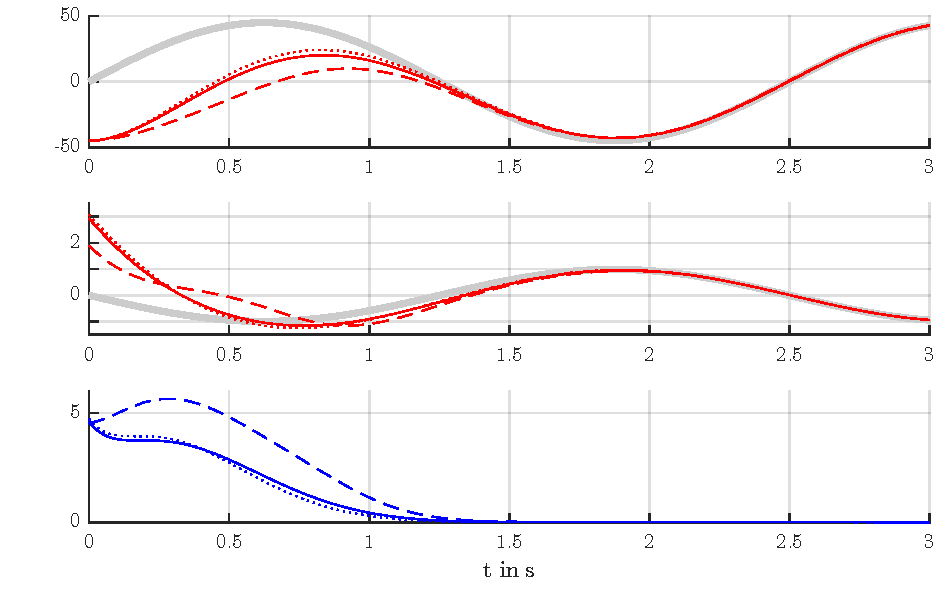
\includegraphics{RevoluteJointSimRes.pdf}}%
\put(0.942384, 2.252072){\rotatebox{90}{\makebox(0,0)[t]{\smash{$\totalEnergyC$ in $\unit{J}$}}}}%
\put(0.942384, 5.425047){\rotatebox{90}{\makebox(0,0)[t]{\smash{$\tau$ in $\unit{Nm}$}}}}%
\put(0.648402, 8.598021){\rotatebox{90}{\makebox(0,0)[t]{\smash{$\jointAngle$ in $\unit{DEG}$}}}}%
\end{picture}%
\endgroup%
 \caption{Simulation result for the revolute joint: gray line: reference, dashed line: particle-based approach, solid line: energy-based approach, dotted line: linear approach}
 \label{fig:RevoluteJointSimRes}
\end{figure}


\paragraph{Linear control.}
Since the model \eqref{eq:RevoluteJointModel} is a linear differential equation, the following linear closed loop equation might also be reasonable
\begin{align}\label{eq:RevoluteJointCtrlLin}
 \Jczz \jointAngleEdd + \sigczz \jointAngleEd + \kapczz \jointAngleE = 0.
\end{align}
The difference between the closed loop \eqref{eq:RevoluteJointClosedLoopApproachEnergy} and \eqref{eq:RevoluteJointCtrlLin} may be visualized by the corresponding phase plots, see \autoref{fig:PhasePlotSO2}:
The linear control law leads to non-smooth phase curves at $\jointAngle = \pm\pi$, which is the consequence of the linear design for a system whose configuration space is actually $\Sphere^1 \ncong \RealNum$.
See \cite[sec.\ 1.2]{Konz:AT} for a deeper discussion.


\paragraph{Simulation results.}
\autoref{fig:RevoluteJointSimRes} shows simulation results comparing the three different approaches \eqref{eq:RevoluteJointClosedLoopApproachParticles}, \eqref{eq:RevoluteJointClosedLoopApproachEnergy} and \eqref{eq:RevoluteJointCtrlLin} tracking a reference $\jointAngleR(t) = \tfrac{\pi}{2}\sin(\tfrac{2\pi}{2.5}t)$.
Evidently, all approaches fulfill the control objective, i.e. the joint angle $\jointAngle$ converges to its reference $\jointAngleR$.


\subsection{Rigid body orientation}\label{sec:CtrlExampleRigidBodyOrientation}
\begin{figure}[ht]
 \centering
 \input{graphics/RigidBodyOrientation.pdf_tex}
 \caption{rigid body fixed at one point}
 \label{fig:RigidBodyOrientation}
\end{figure}

\paragraph{Model.}
Consider a rigid body fixed at one point $\bodyPos{}{} = \const$ as illustrated in \autoref{fig:RigidBodyOrientation}.
Its orientation may be parameterized by the coefficients of the rotation matrix $\R = [\Rx,\Ry,\Rz] \in \SpecialOrthogonalGroup(3)$.
With the angular velocity $\w = \veeMatOp(\R^\top\Rd)$ as velocity coordinates, the inertia matrix $\J$ and the control torques $\tuple{\tau}$ about the body fixed axes, the equations of motion may be written as
\begin{align}
 \Rd = \R \wedOp(\w)
\qquad
 \J\wdot + \wedOp(\w) \J \w &= \tuple{\tau}.
\end{align}

\paragraph{Potential energy.}
Only the parameters $\Jc$, $\sigc$ and $\bodyMOSC{}{}$ contribute to the closed loop kinetics.
Using the attitude error $\RE = \RR^\top \R$ the error potential, its differential and Hessian are
\begin{subequations}
\begin{align}
 \potentialEnergyC &= \tr\big( \wedMatOp(\bodyMOSC{}{}) (\idMat[3] - \RE) \big),
\\
 \genForceStiffC = \differential \potentialEnergyC &= \veeTwoOp(\wedMatOp(\bodyMOSC{}{}) \RE),
\\
 (\differential^2 \potentialEnergyC)|_{\R=\RR} &= \bodyMOSC{}{}.
\end{align} 
\end{subequations}
The potential has the transport map $\sysTransportMap = \RE^\top$, so the velocity error for the energy based approach is $\wE = \w - \RE^\top \wR$ which coincides with the body velocity error.

\paragraph{Particle-based approach.}
The particle-based approach \eqref{eq:CtrlApproachParticles} leads to
\begin{subequations}
\begin{align}
 \genForceInertiaC &= \Jc \wdot - \veeMatOp(\RE^\top \wedMatOp(\Jc)) \RE^\top \wRd
\nonumber\\
 &\hspace{10em}
 + \wedOp(\w) \Jc \w + \veeTwoOp(\wedMatOp(\Jc)\wedOp(\wR)^2\RE)
\\
 \genForceDissC &= \sigc \w - \veeMatOp(\RE^\top \wedMatOp(\sigc)) \RE^\top \wR
\end{align} 
\end{subequations}

\paragraph{Body-based approach.}
The body-based approach \eqref{eq:CtrlApproachBody} leads to 
\begin{subequations}
\begin{align}
 \genForceInertiaC &= \Jc \wEd + \wedOp(\wE) \Jc \wE
\\
 \genForceDissC &= \sigc \wE.
\end{align} 
\end{subequations}
The corresponding control law coincides with the one proposed in \cite{Koditschek:TotalEnergy}.
The total energy $\totalEnergyC = \tfrac{1}{2} \wE^\top \Jc \wE + \potentialEnergyC$ with $\totalEnergyCd = -\wE^\top \sigc \wE$ serves as a Lyapunov function for the closed loop.

\paragraph{Energy-based approach.}
For the energy-based approach \eqref{eq:desiredErrorKineticsEnergy} leads to
\begin{subequations}
\begin{align}
 \genForceInertiaC &= \Jc \wEd + \wedOp(\wedMatOp(\Jc) \w) \wE
\\
 \genForceDissC &= \sigc \wE.
\end{align} 
\end{subequations}
The corresponding control law coincides with one proposed in \cite{Bullo:TrackingAutomatica}.
The total energy is the same as the one for the body based approach.
The two approaches only differ in the gyroscopic terms.
% \begin{align}
%  \gyroForceC 
% % &= \big[ \ConnCoeffLC{\LidxI}{\LidxII}{\LidxIII} \sysVelCoeff{\LidxIII} \sysVelCoeffE{\LidxII} \big]
% % = \big[ \tfrac{1}{2}\big( \BoltzSym{\LidxV}{\LidxI}{\LidxII} \sysInertiaMatCoeffC{\LidxV\LidxIII} + \BoltzSym{\LidxV}{\LidxI}{\LidxIII} \sysInertiaMatCoeffC{\LidxV\LidxII} - \BoltzSym{\LidxV}{\LidxII}{\LidxIII} \sysInertiaMatCoeffC{\LidxV\LidxI} \big) \sysVelCoeff{\LidxIII} \sysVelCoeffE{\LidxII} \big]
% %\nonumber\\
%  &= \tfrac{1}{2} \big( \wedOp(\wE)\Jc \w + \wedOp(\w) \Jc \wE - \Jc \wedOp(\w) \wE \big)
%  = \wedOp(\Jpc \w) \wE
% \end{align}
% Note that $\wedOp(\Jpc \w) \w = \wedOp(\w) \Jpc \w$.

% The explicit control law can be written as
% \begin{align}
%  \tuple{\tau} 
%  &= \J \wdot + \wedOp(\w) \J \w
% \nonumber\\
%  &= \J (\wEd + \RE^\top \wRd - \wedOp(\wE) \RE^\top \wR) + \wedOp(\w) \J \w
% \nonumber\\
%  &= \J (\RE^\top \wRd - \wedOp(\wE) \RE^\top \wR - \Jc^{-1}(\wedOp(\Jpc \w) \wE + \sigc \wE + 2 \veeOp(\kappc \RE))) + \wedOp(\w) \J \w
% \nonumber\\
%  &= \J \big( \RE^\top \wRd - \wedOp(\w) \RE^\top \wR - \Jc^{-1}\wedOp(\w)\Jc \w + \Jc^{-1}\wedOp(\Jpc \w) \RE^\top \wR \big) + \wedOp(\w) \J \w
% \nonumber\\ 
%  &\qquad - \J \Jc^{-1} \big( \sigc \wE + 2 \veeOp(\kappc \RE) \big)
% % \nonumber\\
% %  &= \Jc \R^\top \RR \wRd - \big(\Jc \wedOp(\w) + \wedOp(\Jpc \w)\big) \R^\top \RR \wR
% % \nonumber\\
% %  &\qquad- \sigc (\w - \R^\top \RR \wR) - 2 \veeOp(\kappc \RR^\top \R)
% \end{align}


\paragraph{Linearization.}
For a small error to the reference we have
\begin{align}
 \R = \RR + \RR \wedOp(\LinErrorCoord),
\qquad
 \w = \wR + \LinErrorCoordd,
\qquad
 \Jc \LinErrorCoorddd + \sigc \LinErrorCoordd + \kapc \LinErrorCoord = 0.
\end{align}

\subsection{Planar rigid body}\label{sec:CtrlPlanarRigidBody}
A planar rigid body is a free rigid body in two dimensional space, i.e.\ it can translate in two dimensions and rotate about an perpendicular axis as illustrated in \autoref{fig:PlanarRigidBody}.
The model equations as well as the closed loop equations could be directly derived from the three dimensional rigid body by setting e.g.\ $\vz=0$, $\wx=\wy=0$ and removing the trivial equations.
However it might be still instructive to display the resulting equations.

\begin{figure}[ht]
 \centering
 \input{graphics/PlanarRigidBody.pdf_tex}
 \caption{model of the planar rigid body}
 \label{fig:PlanarRigidBody}
\end{figure}

\paragraph{Coordinates and kinematics.}
As configuration coordinates $\sysCoord$ we use the position $\rx,\ry$ and the sine $\sa$ and cosine $\ca$ of the angle $\alpha$.
Consequently we have to impose the constraint $\ca^2+\sa^2-1 = 0$ on the configuration coordinates.
As velocity coordinates $\sysVel$ we use the components $\vx, \vy$ of the translational velocity w.r.t.\ the body fixed frame as illustrated in \autoref{fig:PlanarRigidBody} and the angular velocity $\wz=\dot{\alpha}$.
This kinematic relation is
\begin{align}
 \ddt
 \underbrace{\begin{bmatrix} \rx \\ \ry \\ \sa \\ \ca \end{bmatrix}}_{\sysCoord}
 = 
 \underbrace{\begin{bmatrix} \ca & -\sa & 0 \\ \sa & \ca & 0 \\ 0 & 0 & \ca \\ 0 & 0 & -\sa \end{bmatrix}}_{\kinMat}
 \underbrace{\begin{bmatrix} \vx \\ \vy \\ \wz \end{bmatrix}}_{\sysVel}
\end{align}
The rigid body configuration $\bodyHomoCoord{0}{1}$ and the resulting body Jacobian $\bodyJac{0}{1}$ w.r.t.\ the chosen velocity coordinates are
\begin{align}
 \bodyHomoCoord{0}{1} = \begin{bmatrix} \ca & -\sa & 0 & \rx \\ \sa & \ca & 0 & \ry \\ 0 & 0 & 1 & 0 \\ 0 & 0 & 0 & 1 \end{bmatrix},
\qquad
 \bodyJac{0}{1} = \begin{bmatrix} 1 & 0 & 0 \\ 0 & 1 & 0 \\ 0 & 0 & 0 \\ 0 & 0 & 0 \\ 0 & 0 & 0 \\ 0 & 0 & 1 \end{bmatrix}
\end{align}

\paragraph{Kinetic equation.}
Let the rigid body have the total mass $\m$, the moment of inertia $\Jz$ and the coordinates $\sx,\sy$ of the center of mass w.r.t.\ the body fixed frame.
As control input consider the forces $\Fx, \Fy$ and the torque $\tauz$ as displayed in \autoref{fig:PlanarRigidBody}.
The resulting kinetic equation is
\begin{align}
 \underbrace{\begin{bmatrix} \m & 0 & -\m\sy \\ 0 & \m & \m\sx \\ -\m\sy & \m\sx & \Jz \end{bmatrix}}_{\sysInertiaMat}
 \underbrace{\begin{bmatrix} \vxd \\ \vyd \\ \wzd \end{bmatrix}}_{\sysVeld}
 +
% \underbrace{
 \begin{bmatrix} -m(\vy + \sx\wz) \wz \\ m(\vx-\sy\wz)\wz \\ \m(\sx\vx+\sy\vy)\wz \end{bmatrix}
% }_{\gyroForce}
%  +
%  \underbrace{\begin{bmatrix} m g \sin\tiltAngle \\ m g \cos\tiltAngle \\ 0 \end{bmatrix}}_{\differential \potentialEnergy}
 =
 \underbrace{\begin{bmatrix} \Fx \\ \Fy \\ \tauz \end{bmatrix}}_{\sysInput}.
\end{align}

\paragraph{Control parameters.}
For the controlled kinetics we chose the following non-zero parameters
\begin{align}\label{eq:CtrlParamPlanarRigidBody}
 \bodyMassC{0}{1}, \bodyDamping{0}{1}, \bodyStiffness{0}{1} \in \RealNum^+,
\quad
 \bodyCOMCoeffC{0}{1}{\idxX}, \bodyCOMCoeffC{0}{1}{\idxY}, \bodyCODCoeffC{0}{1}{\idxX}, \bodyCODCoeffC{0}{1}{\idxY}, \bodyCOSCoeffC{0}{1}{\idxX}, \bodyCOSCoeffC{0}{1}{\idxY} \in \RealNum,
\quad
 \bodyMOICoeffC{0}{1}{\idxZ}, \bodyMODCoeffC{0}{1}{\idxZ}, \bodyMOSCoeffC{0}{1}{\idxZ} \in \RealNum^+ .
\end{align}
Since all parameters are associated with the configuration $\bodyHomoCoord{0}{1}$, we drop the indices in the following, i.e.\ $\mc = \bodyMassC{0}{1}$.

\paragraph{Potential.}
The potential, resulting from the chosen parameters \eqref{eq:CtrlParamPlanarRigidBody}, and its derivatives are
\begin{subequations}
\begin{align}
 \potentialEnergyC &= \tfrac{1}{2} \kc (\rx\!-\!\rxR)^2 + \tfrac{1}{2} \kc (\ry\!-\!\ryR)^2 + \kapcz (1-\caE)
\nonumber\\
 &\qquad+ \kc\hcx(\ca\!-\!\caR)(\rx\!-\!\rxR) - \kc\hcy(\sa\!-\!\saR)(\rx\!-\!\rxR)
\nonumber\\
 &\qquad+ \kc\hcy(\ca\!-\!\caR)(\ry\!-\!\ryR) - \kc\hcx(\sa\!-\!\saR)(\ry\!-\!\ryR)
\label{eq:CtrlPotentialPlanarRigidBody}\\
 \differential \potentialEnergyC &= 
 \begin{bmatrix}
  \kc( \ca(\rx\!-\!\rxR) + \sa(\ry\!-\!\ryR) + \hcx(1-\caE) - \hcy\saE) \\
  \kc(-\sa(\rx\!-\!\rxR) + \ca(\ry\!-\!\ryR) + \hcx\saE + \hcy(1-\caE)) \\
  \kc( (\hcx\ca+\hcy\sa) (\ry\!-\!\ryR) - (\hcy\ca+\hcx\sa) (\rx\!-\!\rxR) ) + \kapcz\saE
 \end{bmatrix}
\\
 \differential^2 \potentialEnergyC |_{\idxRef} &=
 \begin{bmatrix}
  \kc & 0 & -\kc\hcy \\
  0 & \kc & \kc\hcx \\
  -\kc\hcy & \kc\hcx & \kapcz
 \end{bmatrix}
\end{align}
\end{subequations}
The sine and cosine of the angle error $\alpha-\alpha_{\idxRef}$ are introduced just for readability
\begin{align}\label{eq:ErrorCoordPlanarRigidBody}
 \caE = \ca \caR + \sa \saR = \cos(\alpha-\alpha_{\idxRef}),
\qquad
 \saE = \sa \caR - \ca \saR = \sin(\alpha-\alpha_{\idxRef}).
\end{align}
From the Hessian $\differential^2 \potentialEnergyC |_{\idxRef}$ at the critical point $\sysCoord=\sysCoordR$ one can see that (local) positive definiteness requires $\kapcz > \kc (\hcx^2+\hcy^2)$.
We will encounter the analog requirement for the controlled moment of inertia $\Jcz$ and damping $\sigcz$.

A transport map for \eqref{eq:CtrlPotentialPlanarRigidBody} is given by\footnotemark
\begin{align}\label{eq:sysVelEPlanarRigidBody}
 \underbrace{\begin{bmatrix} \vxE \\ \vyE \\ \wzE \end{bmatrix}}_{\sysVelE}
 =
 \underbrace{\begin{bmatrix} \vx \\ \vy \\ \wz \end{bmatrix}}_{\sysVel}
 - 
 \underbrace{\begin{bmatrix}
  \caE & \saE & \sa(\rx \!-\! \rxR) - \ca(\ry \!-\! \ryR) \\
  -\saE & \caE & \ca(\rx \!-\! \rxR) + \sa(\ry \!-\! \ryR) \\
  0 & 0 & 1 
 \end{bmatrix}}_{\sysTransportMap}
 \underbrace{\begin{bmatrix} \vxR \\ \vyR \\ \wzR \end{bmatrix}}_{\sysVelR}.
\end{align}
\footnotetext{
An alternative transport map corresponding to \eqref{eq:RigidBodyAlternativeTransportMap} is
\begin{align}
 \sysTransportMap = \begin{bmatrix}
   \caE & \saE & \hcx\saE - \hcy(\caE - 1) \\
  -\saE & \caE & \hcx(\caE - 1) + \hcy\saE \\
  0 & 0 & 1 
 \end{bmatrix}.
\end{align}
}

\paragraph{Particle-based approach.}
The damping and inertia force using the particle based approach are:
\begin{subequations}
\begin{align}
 \genForceDissC &=
 \underbrace{\begin{bmatrix} \dc & 0 &-\dc\,\lcy \\ 0 & \dc & \dc\,\lcx \\ -\dc\,\lcy & \dc\,\lcx & \sigcz \end{bmatrix}}_{\sysDissMat}
 \underbrace{\begin{bmatrix} \vx \\ \vy \\ \wz \end{bmatrix}}_{\sysVel}
\nonumber\\
 &\qquad-
 \begin{bmatrix} \dc\caE & \dc\saE & \dc(\lcx\saE-\lcy\caE) \\ -\dc\saE & \dc\caE & \dc(\lcx\caE+\lcy\saE) \\ -\dc(\lcx\saE+\lcy\caE) & \dc(\lcx\caE-\lcy\saE) & \sigcz\caE \end{bmatrix}
 \underbrace{\begin{bmatrix} \vxR \\ \vyR \\ \wzR \end{bmatrix}}_{\sysVelR},
\\
 \genForceInertiaC &=
 \underbrace{\begin{bmatrix} \mc & 0 &-\mc\,\scy \\ 0 & \mc & \mc\,\scx \\ -\mc\,\scy & \mc\,\scx & \sigcz \end{bmatrix}}_{\sysDissMat}
 \underbrace{\begin{bmatrix} \vxd \\ \vyd \\ \wzd \end{bmatrix}}_{\sysVeld}
 +
 \begin{bmatrix} -\mc(\vy + \scx\wz) \wz \\ \mc(\vx-\scy\wz)\wz \\ \mc(\scx\vx+\scy\vy)\wz \end{bmatrix}
\nonumber\\
 &\qquad-
 \begin{bmatrix} \mc\caE & \mc\saE & \mc(\scx\saE-\scy\caE) \\ -\mc\saE & \mc\caE & \mc(\scx\caE+\scy\saE) \\ -\mc(\scx\saE+\scy\caE) & \mc(\scx\caE-\scy\saE) & \sigcz\caE \end{bmatrix}
 \underbrace{\begin{bmatrix} \vxRd \\ \vyRd \\ \wzRd \end{bmatrix}}_{\sysVelRd}
\nonumber\\
 &\qquad- 
 \begin{bmatrix} -\mc((\vyR + \scx\wzR)\caE - (\vxR-\scy\wzR)\saE) \wzR \\ \mc((\vyR + \scx\wzR)\saE + (\vxR-\scy\wzR)\caE) \wzR \\ \mc((\scx\vxR+\scy\vyR)\caE - (\scy\vxR-\scx\vyR)\saE)\wzR + \Jcz\saE\wzR^2 \end{bmatrix}.
\end{align}
\end{subequations}
The corresponding total energy as defined in \eqref{eq:SolCtrlGaussPrinciple}, is not a Lyapunov function for the closed loop. 

\paragraph{Body-based approach.}
The damping and inertia force using the body-based approach are:
\begin{subequations}
\begin{align}
 \genForceDissC &= \underbrace{\begin{bmatrix} \dc & 0 &-\dc\,\lcy \\ 0 & \dc & \dc\,\lcx \\ -\dc\,\lcy & \dc\,\lcx & \sigcz \end{bmatrix}}_{\sysDissMat}
 \underbrace{\begin{bmatrix} \vxE \\ \vyE \\ \wzE \end{bmatrix}}_{\sysVelE}
\\
 \genForceInertiaC &= \underbrace{\begin{bmatrix} \mc & 0 & -\mc\scy \\ 0 & \mc & \mc\scx \\ -\mc\scy & \mc\scx & \Jcz \end{bmatrix}}_{\sysInertiaMat}
 \underbrace{\begin{bmatrix} \vxEd \\ \vyEd \\ \wzEd \end{bmatrix}}_{\sysVelEd}
 + \begin{bmatrix} 0 & -\mc\wzE & -\mc\scx\wzE \\ \mc\wzE & 0 & -\mc\scy\wzE \\ \mc\scx\wzE & \mc\scy\wzE & 0 \end{bmatrix}
 \begin{bmatrix} \vxE \\ \vyE \\ \wzE \end{bmatrix}
\end{align} 
\end{subequations}
where the velocity error $\sysVelE$ was defined in \eqref{eq:sysVelEPlanarRigidBody}.
The total energy $\totalEnergyC = \tfrac{1}{2} \sysVelE^\top \sysInertiaMat \sysVelE + \potentialEnergyC$ is a Lyapunov function for the closed loop.

\paragraph{Energy-based approach.}
The damping and inertia forces using the energy-based approach are:
\begin{subequations}
\begin{align}
 \genForceDissC &= \underbrace{\begin{bmatrix} \dc & 0 &-\dc\,\lcy \\ 0 & \dc & \dc\,\lcx \\ -\dc\,\lcy & \dc\,\lcx & \sigcz \end{bmatrix}}_{\sysDissMat}
 \underbrace{\begin{bmatrix} \vxE \\ \vyE \\ \wzE \end{bmatrix}}_{\sysVelE},
\\
 \genForceInertiaC &= \underbrace{\begin{bmatrix} \mc & 0 & -\mc\scy \\ 0 & \mc & \mc\scx \\ -\mc\scy & \mc\scx & \Jcz \end{bmatrix}}_{\sysInertiaMat}
 \underbrace{\begin{bmatrix} \vxEd \\ \vyEd \\ \wzEd \end{bmatrix}}_{\sysVelEd}
 + \begin{bmatrix} 0 & -\mc\wz & -\mc\scx\wz \\ \mc\wz & 0 & -\mc\scy\wz \\ \mc\scx\wz & \mc\scy\wz & 0 \end{bmatrix}
 \begin{bmatrix} \vxE \\ \vyE \\ \wzE \end{bmatrix}.
\end{align} 
\end{subequations}
The total energy $\totalEnergyC = \tfrac{1}{2} \sysVelE^\top \sysInertiaMat \sysVelE + \potentialEnergyC$ coincides with the total energy for the body-based approach and is a Lyapunov function for this closed loop as well.
Note that the two approaches do differ in the gyroscopic terms, so do lead to different solutions of the closed loop dynamics.

\paragraph{Simulation result.}
In \autoref{sec:DecouplingRigidBody} we will give and discuss a simulation result for the special parameter choice $\scx=\lcx=\hcx=0$ and $\scy=\lcy=\hcy=0$.


\subsection{Free rigid body: decoupling of translational and rotational motion}\label{sec:DecouplingRigidBody}
The closed loop equations for a (free) three dimensional rigid body were given in \autoref{sec:CtrlApproachParticlesSingleBody}, \autoref{sec:CtrlApproachBodySingleBody} and \autoref{sec:CtrlApproachEnergySingleBody}.
The reduced equations for the planar case were given in \autoref{sec:CtrlPlanarRigidBody}.
For most applications we like to \textit{decouple} the translational and the rotational motion of the body.
%What this means and how it is achieved is discussed in this subsection.

Observing the closed loop equations one can see immediately that the coupling terms vanish if $\sc=\lc=\hc=\tuple{0}$, i.e.\ the the chosen body fixed point $\r$ coincides with the center of mass, damping and stiffness.
Then the rotational dynamics are identical to the closed loop given in \autoref{sec:CtrlExampleRigidBodyOrientation} (\autoref{sec:CtrlExampleRevoluteJoint} for the planar case), so are indeed decoupled/independent from the translational motion.

\paragraph{Translational dynamics.}
For the translational dynamics the situation is more difficult:
Introduce $\tuple{e} = \r-\rR$ as the components of the position error w.r.t.\ the inertial frame and $\rE = \RR^\top(\r-\rR)$ as the components w.r.t.\ the reference frame.
The translational dynamics for the different approaches and given transport map are equivalent to
\begin{subequations}\label{eq:RigidBodyPosErrorDyn}
\begin{align}
 &\text{particle-based:}&
 \mc\ddot{\tuple{e}} + \dc\dot{\tuple{e}} + \kc\tuple{e} &= \tuple{0}
\\
 &\text{body-based:}&
 \mc\rEdd + \dc\rEd + \kc\rE &= \tuple{0}
\\
 &\text{energy-based:}&
 \mc \big(\rEdd + \wedOp(\wR) \rEd \big) + \dc\rEd + \kc\rE &= \tuple{0}
 \label{eq:RigidBodyPosErrorDynApproach1}
% \\
%  &\text{approach 1 with \eqref{eq:RigidBodyAlternativeTransportMap}:}&
%  \mc\ddot{\tuple{e}} + \dc\dot{\tuple{e}} + \kc\tuple{e} &= \tuple{0}
\end{align}
\end{subequations}
% Obviously, for approach 1 with the transport map from \eqref{eq:RigidBodyAlternativeTransportMap} and approach 2, the error components $\tuple{e}$ w.r.t.\ the inertial frame obey linear dynamics.
% The same holds for approach 3 for the error components $\rE$ w.r.t.\ the reference frame.
% There is no transformation of the error coordinates to achieve this for approach 1 with the transport map from \eqref{eq:TransportMapRigidBody}.
% It is crucial to notice that all equations are indeed independent from the actual orientation $\R$ and angular velocity $\w$, but some do depend on their \textit{reference} $\RR$ and $\wR$.

\paragraph{Translational energy.}
For the rigid body we can split the total energy $\totalEnergyC = \totalEnergyC_{\r} + \totalEnergyC_{\R}$ into a part associated with the position $\totalEnergyC_{\r}$ and one associated with the orientation $\totalEnergyC_{\R}$.
The rotational energies for the corresponding approaches coincide with the ones given in \autoref{sec:CtrlExampleRigidBodyOrientation} (\autoref{sec:CtrlExampleRevoluteJoint} for the planar case).
The translational energies and their change along the solutions of \eqref{eq:RigidBodyPosErrorDyn} are
\begin{subequations}
\begin{align}
 &\text{particle-based:}&
 \totalEnergyC_{\r} &= \tfrac{1}{2} \kc \norm{\tuple{e}}^2 + \tfrac{1}{2} \mc \norm{\dot{\tuple{e}}}^2,&
 \dot{\totalEnergyC}_{\r} &= -\dc\norm{\dot{\tuple{e}}}^2
\\
 &\text{body-based:}&
 \totalEnergyC_{\r} &= \tfrac{1}{2} \kc \norm{\rE}^2 + \tfrac{1}{2} \mc \norm{\rEd}^2,&
 \dot{\totalEnergyC}_{\r} &= -\dc\norm{\rEd}^2 
\\
 &\text{energy-based:}&
 \totalEnergyC_{\r} &= \tfrac{1}{2} \kc \norm{\rE}^2 + \tfrac{1}{2} \mc \norm{\rEd}^2,&
 \dot{\totalEnergyC}_{\r} &= -\dc\norm{\rEd}^2 
%  &\text{approach 1 with \eqref{eq:RigidBodyAlternativeTransportMap}:}&
%  \totalEnergyC_{\r} &= \tfrac{1}{2} \kc \norm{\tuple{e}}^2 + \tfrac{1}{2} \mc \norm{\dot{\tuple{e}}}^2,&
%  \dot{\totalEnergyC}_{\r} &= -\dc\norm{\dot{\tuple{e}}}^2 
\end{align}
\end{subequations}
For their comparison note that
\begin{align}
 \norm{\tuple{e}} = \norm{\rE},
\qquad
 \norm{\dot{\tuple{e}}} = \norm{\rEd + \wedOp(\wR) \rE}.
\end{align}

The crucial observation is that for all approaches the translational dynamics and energy are indeed independent of the actual orientation $\R$ and its velocity $\w$, but for some approaches they depend on their \textit{reference} $\RR$ and $\wR$.
For a constant reference orientation $\RR = \const$ and consequently $\wR = \tuple{0}$ all four approaches are equivalent.
Furthermore it is worth noting that the error dynamics as well as the energies are invariant to the reference trajectory $t\mapsto\rR(t)$ for the position.

\begin{figure}
 \centering
 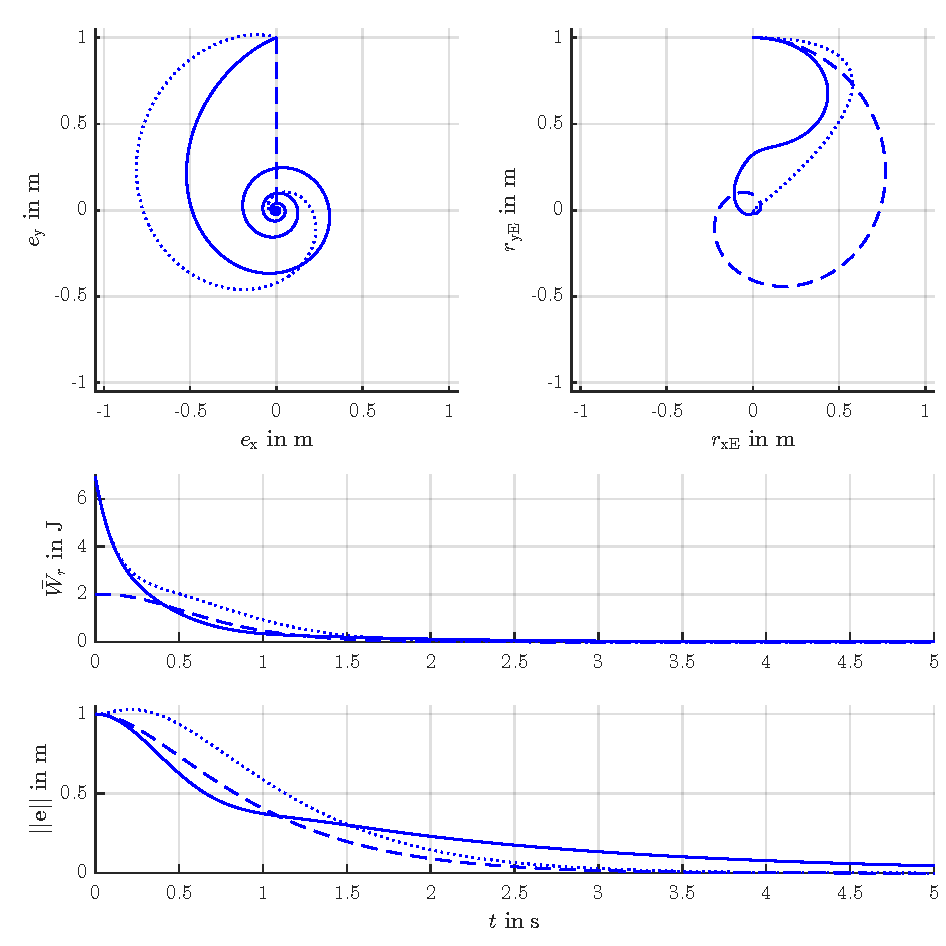
\includegraphics{PlanarRigidBody/RBCtrlPosError}
 \caption{Simulation result for the planar rigid body. The solid line: energy-based approach with $\sysTransportMap = \Ad{\bodyHomoCoord{}{}^{-1}\bodyHomoCoordR{}{}}$, dashed line: particle-based approach, dotted line: body-based approach.}
 \label{fig:RBCtrlPosError}
\end{figure}

\paragraph{Simulation.}
The difference between these cases will be discussed on simulation results for the simpler, yet as illustrative, example of a planar rigid body:
The reference configuration is $\rxR(t) = \ryR(t) = 0$ and $\alpha_{\idxRef}(t) = \pi t$ which yields the constant reference velocity $\sysVelR(t) = [0,0,\pi]$.
The control parameters are set to $\mc=1$, $\dc=4$, $\kc=4$ (neglecting the units).
The roots of the characteristic polynomial of \eqref{eq:RigidBodyPosErrorDynApproach1} are $\lambda \approx \{-0.5 \pm 0.6\mathrm{i}, -3.5 \pm 3.7\mathrm{i} \}$, resulting from the control parameters as well as the constant angular velocity $\wzR=\pi$.
The characteristic polynomial for the other approaches is independent of the reference trajectory and has a quadruple root at $\lambda = -2$.

\autoref{fig:RBCtrlPosError} shows the simulation result for the initial conditions $\rx(0) = 0, \ry(0) = 1$, $\alpha(0) = 0$ and $\sysVel(0) = \tuple{0}$.
Observing from the inertial frame, top left of \autoref{fig:RBCtrlPosError}, for approach 2 the body follows a straight line to its reference position, whereas for the other approaches spiral around it.
Observing from the reference frame, top right of \autoref{fig:RBCtrlPosError}, for approach 3 the body follows a direct path, given the initial velocity.
The middle graph in \autoref{fig:RBCtrlPosError} shows the evolution of the translational energy $\totalEnergyC_{\r}$.
The difference in the initial values results from $\dot{\tuple{e}}(0) = \tuple{0}$, but $\rEd(0) \neq \tuple{0}$.
The bottom graph in \autoref{fig:RBCtrlPosError} shows the evolution of the euclidean distance $\norm{\tuple{e}} = \norm{\rE}$.
The rate of convergence for approach 2 and 3 are the same as could be expected from having the same characteristic polynomial.

Even though the energy based approach with the transport map from \eqref{eq:TimeDerivativeRigidBodxPotential} might be mathematically the most elegant solution, its simulation result is not intuitive.
Which approach is most desirable, depends given application.
For indoor robots (like the multicopters discussed in the next chapter) it is probably most desirable if it corrects its position error following a straight line in the inertial frame.


% \paragraph{Approach 2}
% \begin{align*}
%  \mc (\vd + \wedOp(\w) \v - \RE^\top (\vRd + \wedOp(\wR)\vR) ) + \dc(\v - \RE^\top\vR) + \kc \R^\top(\r-\rR) &= \tuple{0}
% % \\
% %  \mc (\R^\top\rdd - \wedOp(\w)\R^\top \rd + \wedOp(\w) \R^\top \rd - \R^\top\RR (\RR^\top\rRdd - \wedOp(\wR)\RR^\top \rRd + \wedOp(\wR)\RR^\top\rRd) ) + \dc\R^\top(\rd - \rRd) + \kc \R^\top(\r-\rR) &= \tuple{0}
% \\
%  \Leftrightarrow\qquad
%  \mc\ddot{\tuple{e}} + \dc\dot{\tuple{e}} + \kc\tuple{e} &= \tuple{0}
% \end{align*}
% 
% 
% \paragraph{Approach 3}
% \begin{align*}
%  \mc \big(\vEd + \wedOp(\wE) \vE\big) + \dc\vE + \kc \R^\top(\r-\rR) &= \tuple{0}
% \\
%  \Leftrightarrow \qquad
%  \mc \big( \ddot{\tuple{e}} - 2\wedOp(\RR \wR) \dot{\tuple{e}} - \big(\wedOp(\RR \wRd) - \wedOp(\RR \wR)^2\big) \tuple{e} \big)\qquad&
% \\+ \dc\big(\dot{\tuple{e}} - \wedOp(\RR \wR) \tuple{e} \big) + \kc\tuple{e} &= \tuple{0}
% \\
%  \mc\rEdd + \dc\rEd + \kc\rE &= \tuple{0}
% \end{align*}
% 
% 
% \paragraph{Error coordinates}
% \begin{align}
%  \underbrace{\begin{bmatrix} \RE & \rE \\ \mat{0} & 1 \end{bmatrix}}_{\bodyHomoCoordE{}{}} 
%  &= \underbrace{\begin{bmatrix} \RR^\top \R & \RR^\top (\r - \rR) \\ \mat{0} & 1 \end{bmatrix}}_{\bodyHomoCoordR{}{}^{-1}\bodyHomoCoord{}{}},&
% %  &= \underbrace{\begin{bmatrix} \RR^\top & -\RR^\top \rR \\ \mat{0} & 1 \end{bmatrix}}_{\bodyHomoCoordR{}{}^{-1}} 
% %  \underbrace{\begin{bmatrix} \R & \r \\ \mat{0} & 1 \end{bmatrix}}_{\bodyHomoCoord{}{}}
%  \underbrace{\begin{bmatrix} \vE \\ \wE \end{bmatrix}}_{\bodyVelE{}{}} 
%  &= \underbrace{\begin{bmatrix} \v \\ \w \end{bmatrix}}_{\bodyVel{}{}} 
%  - \underbrace{\begin{bmatrix} \RE^\top & -\RE^\top \wedOp\rE \\ \mat{0} & \RE^\top \end{bmatrix}}_{\Ad{\bodyHomoCoordE{}{}^{-1}}} 
%  \underbrace{\begin{bmatrix} \vR \\ \wR \end{bmatrix}}_{\bodyVelR{}{}}.
% \end{align}
% 
% \begin{align*}
%  \vE &= \v - \R^\top \RR \vR + \R^\top \RR \wedOp(\RR^\top(\r-\rR)) \wR,
% \\
%  &= \R^\top \big(\dot{\tuple{e}} - \wedOp(\RR \wR) \tuple{e} \big),
% \\
%  &= \RE^\top \rEd,
% \\
%  \wE &= \w - \RE^\top \wR
% \end{align*}
% 
% 
% \paragraph{Approach 1}
% \begin{align*}
%  \mc \big(\vEd + \wedOp(\w) \vE\big) + \dc\vE + \kc \R^\top(\r-\rR) &= \tuple{0}
% \\
% %  \mc (\R^\top \rdd - \wedOp(\w)\R^\top \rd + \wedOp(\w)\R^\top (\rRd + \wedOp(\RR \wR) (\r-\rR))&
% % \\ -\R^\top (\rRdd + \wedOp(\RR \wRd) (\r-\rR) + \wedOp(\RR \wR) (\rd-\rRd))&
% % \\ + \wedOp(\w) (\R^\top\rd - \R^\top (\rRd + \wedOp(\RR \wR) (\r-\rR))))&
% % \\ + \dc(\R^\top\rd - \R^\top (\rRd + \wedOp(\RR \wR) (\r-\rR))) + \kc \R^\top(\r-\rR) &= \tuple{0}
% % \\
%  \Leftrightarrow\qquad 
%  \mc \big(\ddot{\tuple{e}} - \wedOp(\RR \wR) \dot{\tuple{e}} - \wedOp(\RR \wRd) \tuple{e} \big) + \dc(\dot{\tuple{e}} - \wedOp(\RR \wR) \tuple{e}) + \kc \tuple{e} &= \tuple{0}
% \\
%  \Leftrightarrow\qquad 
%  \mc \big(\rEdd + \wedOp(\wR) \rEd \big) + \dc\rEd + \kc\rE &= \tuple{0}
% \end{align*}
% 
% \paragraph{Approach 2}
% \begin{align*}
%  \mc (\vd + \wedOp(\w) \v - \RE^\top (\vRd + \wedOp(\wR)\vR) ) + \dc(\v - \RE^\top\vR) + \kc \R^\top(\r-\rR) &= \tuple{0}
% % \\
% %  \mc (\R^\top\rdd - \wedOp(\w)\R^\top \rd + \wedOp(\w) \R^\top \rd - \R^\top\RR (\RR^\top\rRdd - \wedOp(\wR)\RR^\top \rRd + \wedOp(\wR)\RR^\top\rRd) ) + \dc\R^\top(\rd - \rRd) + \kc \R^\top(\r-\rR) &= \tuple{0}
% \\
%  \Leftrightarrow\qquad
%  \mc\ddot{\tuple{e}} + \dc\dot{\tuple{e}} + \kc\tuple{e} &= \tuple{0}
% \end{align*}
% 
% 
% \paragraph{Approach 3}
% \begin{align*}
%  \mc \big(\vEd + \wedOp(\wE) \vE\big) + \dc\vE + \kc \R^\top(\r-\rR) &= \tuple{0}
% \\
%  \Leftrightarrow \qquad
%  \mc \big( \ddot{\tuple{e}} - 2\wedOp(\RR \wR) \dot{\tuple{e}} - \big(\wedOp(\RR \wRd) - \wedOp(\RR \wR)^2\big) \tuple{e} \big)\qquad&
% \\+ \dc\big(\dot{\tuple{e}} - \wedOp(\RR \wR) \tuple{e} \big) + \kc\tuple{e} &= \tuple{0}
% \\
%  \mc\rEdd + \dc\rEd + \kc\rE &= \tuple{0}
% \end{align*}

\subsection{SCARA robot}\label{sec:CtrlScara}
As a simple example of a multi-body system we consider a SCARA robot as displayed in \autoref{fig:Scara}.
For the sake of demonstration we neglect the vertical axis and the tool orientation.
The remaining two axis are sufficient to position a tool (red point in \autoref{fig:Scara}) in the workspace (green shaded area).

\begin{figure}[ht]
 \centering
 \input{graphics/Scara.pdf_tex}
 \caption{A Scara robot and its mechanical model (image \url{www.epson.com})}
 \label{fig:Scara}
\end{figure}

\paragraph{Model.}
The model consists of two rigid bodies constraint by two revolute joints.
A reasonable choice of coordinates are the relative joint angles $\sysCoord = [\jointAngle[1], \jointAngle[2]]^\top$ and their derivatives $\sysVel = [\jointAngled[1], \jointAngled[2]]^\top$.
The rigid body configurations are
\begin{subequations}
\begin{align}
 \bodyHomoCoord{0}{1} &=
 \begin{bmatrix}
  \cos\jointAngle[1] & -\sin\jointAngle[1] & 0 & 0 \\
  \sin\jointAngle[1] &  \cos\jointAngle[1] & 0 & 0 \\
  0 & 0 & 1 & 0 \\
  0 & 0 & 0 & 1
 \end{bmatrix},&
 \bodyJac{0}{1} &= \begin{bmatrix} 0 & 0 \\ 0 & 0 \\ 0 & 0 \\ 0 & 0 \\ 0 & 0 \\ 1 & 0 \end{bmatrix}
\\
 \bodyHomoCoord{1}{2} &=
 \begin{bmatrix}
  \cos\jointAngle[2] & -\sin\jointAngle[2] & 0 & l_1 \\
  \sin\jointAngle[2] &  \cos\jointAngle[2] & 0 & 0 \\
  0 & 0 & 1 & 0 \\
  0 & 0 & 0 & 1
 \end{bmatrix},&
 \bodyJac{1}{2} &= \begin{bmatrix} 0 & 0 \\ 0 & 0 \\ 0 & 0 \\ 0 & 0 \\ 0 & 0 \\ 0 & 1 \end{bmatrix}
 .
\end{align} 
\end{subequations}

% \autoref{tab:ScaraMdlParam} collects the relevant values inside the body inertia matrices $\bodyInertiaMat{0}{1}{}$, $\bodyInertiaMat{0}{2}{}$ \wrt to the chosen body fixed frames which will later be used for simulation.
% Remark that the joint axis are parallel to the gravity direction and consequently there are no gravitational forces.
% Overall we assume no potential $\potentialEnergy = 0$ and no dissipative influences $\sysDissMat = 0$.
% The only external force on the system are the control forces $\sysInput = [\tau_1, \tau_2]^\top$ that act on the joint axes.

% \begin{table}
% \centering
% \setlength\extrarowheight{1ex}
% \begin{tabular}{rc}
%  \toprule
%  length arm 1 & $l_1 = 0.3\,\unit{m}$ \\
%  length arm 2 & $l_2 = 0.2\,\unit{m}$ \\
%  mass arm 1 & $\bodyMass{0}{1} = 1\,\unit{kg}$ \\
%  mass arm 2 & $\bodyMass{0}{2} = 2\,\unit{kg}$ \\
%  center of mass arm 1 & $\bodyCOMCoeff{0}{1}{1} = \tfrac{l_1}{2} = 0.15\,\unit{m}$, $\bodyCOMCoeff{0}{1}{2} = 0\,\unit{m}$ \\
%  center of mass arm 2 & $\bodyCOMCoeff{0}{2}{1} = \tfrac{l_2}{2} = 0.1\,\unit{m}$, $\bodyCOMCoeff{0}{2}{2} = 0\,\unit{m}$ \\
%  moment of inertia arm 1 & $\bodyMOICoeff{0}{1}{33} = \tfrac{\bodyMass{0}{1}\, l_1^2}{12} = 0.0075\,\unit{kg}\,\unit{m}^2$ \\
%  moment of inertia arm 2 & $\bodyMOICoeff{0}{2}{33} = \tfrac{\bodyMass{0}{2}\, l_2^2}{12} \approx 0.00667\,\unit{kg}\,\unit{m}^2$ \\
%  \bottomrule
% \end{tabular}
% \caption{model parameters for the SCARA robot used for simulation}
% \label{tab:ScaraMdlParam}
% \end{table}

Let $\bodyMOICoeff{}{1}{\idxZ}$ be the moment of inertia of the first body about the first joint and $l_1$ be the distance between the two joints.
The second body has the mass $\bodyMass{}{2}$, the center of mass $(\bodyCOMCoeff{}{2}{\idxX}, \bodyCOMCoeff{}{2}{\idxY})$ and the moment of inertia $\bodyMOICoeff{}{2}{\idxZ}$ about the second joint.
The control forces are the joint torques $\sysInput = [\tau_1, \tau_2]^\top$.
Overall, the equations of motion for the SCARA robot are
% \begin{multline}
%  \begin{bmatrix}
%   \bodyMOICoeff{}{1}{\idxZ} \!+\! \bodyMOICoeff{}{2}{\idxZ} \!+\! \bodyMass{}{2} l_1^2 \!+\! 2 \bodyMass{}{2} l_1 (\bodyCOMCoeff{}{2}{\idxX} \cos\jointAngle[2] \!-\! \bodyCOMCoeff{}{2}{\idxY} \sin\jointAngle[2]) & \bodyMOICoeff{}{2}{\idxZ} \!+\! \bodyMass{}{2} l_1 (\bodyCOMCoeff{}{2}{\idxX} \cos\jointAngle[2] \!-\! \bodyCOMCoeff{}{2}{\idxY} \sin\jointAngle[2]) \\ 
%   \bodyMOICoeff{}{2}{\idxZ} \!+\! \bodyMass{}{2} l_1 (\bodyCOMCoeff{}{2}{\idxX} \cos\jointAngle[2] \!-\! \bodyCOMCoeff{}{2}{\idxY} \sin\jointAngle[2]) & \bodyMOICoeff{}{2}{\idxZ}
%  \end{bmatrix}
%  \begin{bmatrix} \jointAngledd[1] \\ \jointAngledd[2] \end{bmatrix}
% \\
%  +
%  \begin{bmatrix}
%   -\bodyMass{}{2} l_1 \jointAngled[2] (2\jointAngled[1]+\jointAngled[2]) (\bodyCOMCoeff{}{2}{\idxX} \sin\jointAngle[2] \!+\! \bodyCOMCoeff{}{2}{\idxY} \cos\jointAngle[2]) \\
%    \bodyMass{}{2} l_1 \jointAngled[1]^2 (\bodyCOMCoeff{}{2}{\idxX} \sin\jointAngle[2] \!+\! \bodyCOMCoeff{}{2}{\idxY} \cos\jointAngle[2])
%  \end{bmatrix}
%  = \begin{bmatrix} \tau_1 \\ \tau_2 \end{bmatrix}
% \end{multline}
\begin{align}
 \begin{bmatrix}
  \bodyMOICoeff{}{1}{\idxZ} \!+\! \bodyMOICoeff{}{2}{\idxZ} \!+\! \bodyMass{}{2} l_1^2 \!+\! 2 a(\jointAngle[2]) & \bodyMOICoeff{}{2}{\idxZ} \!+\! a(\jointAngle[2]) \\ 
  \bodyMOICoeff{}{2}{\idxZ} \!+\! a(\jointAngle[2]) & \bodyMOICoeff{}{2}{\idxZ}
 \end{bmatrix}
 \begin{bmatrix} \jointAngledd[1] \\ \jointAngledd[2] \end{bmatrix}
 +
 \begin{bmatrix}
   a'(\jointAngle[2]) (2\jointAngled[1] \jointAngled[2] + \jointAngled[2]^2) \\
  -a'(\jointAngle[2]) \jointAngled[1]^2
 \end{bmatrix}
 = \begin{bmatrix} \tau_1 \\ \tau_2 \end{bmatrix}
\end{align}
where
\begin{align}
 a(\jointAngle[2]) &= \bodyMass{}{2} l_1 (\bodyCOMCoeff{}{2}{\idxX} \cos\jointAngle[2] \!-\! \bodyCOMCoeff{}{2}{\idxY} \sin\jointAngle[2]),&
 a'(\jointAngle[2]) &= -\bodyMass{}{2} l_1 (\bodyCOMCoeff{}{2}{\idxX} \sin\jointAngle[2] \!+\! \bodyCOMCoeff{}{2}{\idxY} \cos\jointAngle[2]).
\end{align}

\paragraph{Controller parameterization 1.}
In the following we will discuss two different controller parameterizations for the SCARA.
For the first parameterization the non-zero parameters are
\begin{align}
 \bodyMOSCoeffC{0}{1}{\idxZ}, 
 \bodyMODCoeffC{0}{1}{\idxZ}, 
 \bodyMOICoeffC{0}{1}{\idxZ}, \
 \bodyMOSCoeffC{1}{2}{\idxZ}, 
 \bodyMODCoeffC{1}{2}{\idxZ},
 \bodyMOICoeffC{1}{2}{\idxZ} \in \RealNum > 0.
\end{align}
These parameters are directly associated with the errors $\jointAngleE[i] = \jointAngle[i] - \jointAngleR[i], i=1,2$ of the joint angles.
The resulting potential is
\begin{align}
 \potentialEnergyC = \bodyMOSCoeffC{0}{1}{\idxZ} \big( 1-\cos \jointAngleE[1] \big) + \bodyMOSCoeffC{1}{2}{\idxZ}\big( 1-\cos\jointAngleE[2] \big).
\end{align}
and obeys the transport map $\sysTransportMap = \idMat[2]$.

The resulting controlled kinetics for the body and energy-based approach are
\begin{align}\label{eq:ScaraClosedLoop11}
 \bodyMOICoeffC{i-1}{i}{\idxZ} \jointAngleEdd[i]
 + \bodyMODCoeffC{i-1}{i}{\idxZ} \jointAngleEd[i]
 + \bodyMOSCoeffC{i-1}{i}{\idxZ} \sin \jointAngleE[i]
 = 0, \qquad i=1,2.
\end{align}
%This result is similar (apart from the sine in the potential force which was \fixme{motivated in the example}) to the common approach with computed torque, but here there is a physical interpretation of the control parameters.
%Note also that the consideration of an inertia $\bodyInertiaMat{1}{2}{}$ of arm 2 \wrt arm 1 (instead the inertial frame) is crucial to obtain the system inertia $\sysInertiaMat = \idMat[2]$.
The controlled kinetics for the particle based approach yield
\begin{multline}\label{eq:ScaraClosedLoop12}
 \bodyMOICoeffC{i-1}{i}{\idxZ} \big( \jointAngledd[i] - \jointAngleRdd[i]\cos\jointAngleE[i] - \jointAngleRd[i]^2 \sin\jointAngleE[i] \big)
 + \bodyMODCoeffC{i-1}{i}{\idxZ} \big( \jointAngled[i] - \jointAngleRd[i]\cos\jointAngleE[i] \big)
 + \bodyMOSCoeffC{i-1}{i}{\idxZ} \sin \jointAngleE[i]
 = 0,
\\
 i=1,2.
\end{multline}
With this parameterization the controlled kinetics coincide with two copies of the kinetics of the revolute joint discussed in \autoref{sec:CtrlExampleRevoluteJoint}.


\paragraph{Controller parameterization 2.}
The non-zero parameters for another interesting parameterization of the controller are
\begin{align}
 \bodyStiffnessC{0}{2}, \bodyDampingC{0}{2}, \bodyMassC{0}{2} \in \RealNum > 0,
\quad
 \bodyCOSCoeffC{0}{2}{\idxX} = \bodyCODCoeffC{0}{2}{\idxX} = \bodyCOMCoeffC{0}{2}{\idxX} = l_2.
\end{align}
The resulting potential can be written as
\begin{align}
 \potentialEnergyC(\sysCoord, \sysCoordR) = \tfrac{1}{2} \, \bodyStiffnessC{0}{2} \, \norm{\toolPos(\sysCoord) - \toolPos(\sysCoordR)}^2
\qquad
 \toolPos(\sysCoord) = 
 \begin{bmatrix}
  l_1 \cos \jointAngle[1] + l_2 \cos (\jointAngle[1] \!+\! \jointAngle[2]) \\
  l_1 \sin \jointAngle[1] + l_2 \sin (\jointAngle[1] \!+\! \jointAngle[2]) \\
 \end{bmatrix},
\end{align}
where $\toolPos$ is the position of the tool as illustrated in \autoref{fig:Scara}.
Using the \textit{tool position error} $\sysCoordE(\sysCoord, \sysCoordR) = \toolPos(\sysCoord) - \toolPos(\sysCoordR)$ as error coordinates, we can apply the rule from \eqref{eq:DefErrorTransportMap} to compute the transport map as
\begin{align}
 \sysTransportMap(\sysCoord, \sysCoordR) &= \big( \differential\toolPos (\sysCoord) \big)^{-1} \, \differential \toolPos (\sysCoordR).
\end{align}
% the elements are
% \begin{align*}
%  \sysTransportMapCoeff{1}{1} &= (l_1\sin\jointAngle[2])^{-1} \big( l_1 \sin(\jointAngleE[1]+\jointAngle[2]) + l_2 \sin(\jointAngleE[1]+\jointAngleE[2]) \big)
% \\
%  \sysTransportMapCoeff{1}{2} &= (l_1\sin\jointAngle[2])^{-1} l_2 \sin(\jointAngleE[1]+\jointAngleE[2])
% \\
%  \sysTransportMapCoeff{2}{1} &= (l_1 l_2 \sin\jointAngle[2])^{-1} \big( l_1^2 \sin\jointAngleE[1] + l_2^2 \sin(\jointAngleE[1]+\jointAngleE[2]) + l_1 l_2 ( \sin(\jointAngleE[1]+\jointAngle[2]) - \sin(\jointAngleE[1] - \jointAngleR[2]) ) \big)
% \\
%  \sysTransportMapCoeff{2}{2} &= -(l_1\sin\jointAngle[2])^{-1} \big(l_1 \sin(\jointAngleE[1]-\jointAngleR[2]) + l_2 \sin(\jointAngleE[1]+\jointAngleE[2]) \big).
% \end{align*}
% Note that the symbols $\jointAngleE[i]$ are used only for readability, they have nothing to do with the error velocity $\sysVelE = \sysVel - \sysTransportMap\sysVelR $ in this case.
The determinant of the differential $\det\differential\toolPos(\sysCoord) = \sin\jointAngle[2]$ reflects the well known singularity of the SCARA inverse kinematics, see e.g.\ \cite[example 3.6]{Murray:Robotic}.

The closed loop kinetics for the particle and energy-based approach in terms of the model coordinates $\sysCoord$ and the error velocity $\sysVelE = \sysVel - \sysTransportMap\sysVelR$ are
\begin{subequations}
\begin{multline}
 \underbrace{\bodyMassC{0}{2} \begin{bmatrix}
   l_1^2 + 2 l_1 l_2 \cos\jointAngle[2] + l_2^2 & l_1 l_2\cos\jointAngle[2] + l_2^2 \\
   l_1 l_2 \cos\jointAngle[2] + l_2^2 & l_2^2
 \end{bmatrix}}_{\sysInertiaMatC}
 \sysVelEd
%  + \bodyMassC{0}{2} l_1 l_2 \sin\jointAngle[2] \begin{bmatrix}
%    -\sysVelCoeff{2} \sysVelCoeffE{1} - (\sysVelCoeff{1} + \sysVelCoeff{2}) \sysVelCoeffE{2} \\
%    \sysVelCoeff{1} \sysVelCoeffE{1}
%  \end{bmatrix}
 + \bodyMassC{0}{2} l_1 l_2 \sin\jointAngle[2] 
 \begin{bmatrix}
  -\jointAngled[2] & -\jointAngled[1]-\jointAngled[2] \\
  \jointAngled[1] & 0
 \end{bmatrix}
 \sysVelE
\\
 + \underbrace{\bodyDampingC{0}{2} \begin{bmatrix}
   l_1^2 + 2 l_1 l_2 \cos\jointAngle[2] + l_2^2 & l_1 l_2\cos\jointAngle[2] + l_2^2 \\
   l_1 l_2 \cos\jointAngle[2] + l_2^2 & l_2^2
 \end{bmatrix}}_{\sysDissMatC}
 \sysVelE
\\
 + \underbrace{\bodyStiffnessC{0}{2} \begin{bmatrix}
  l_1^2 \sin\jointAngleE[1] + l_1 l_2 (\sin(\jointAngleE[1]-\jointAngleR[2]) + \sin(\jointAngleE[1]+\jointAngle[2])) + l_2^2 \sin(\jointAngleE[1]+\jointAngleE[2]) \\
  l_1 l_2 (\sin(\jointAngleE[1]+\jointAngle[2]) - \sin(\jointAngle[2])) + l_2^2 \sin(\jointAngleE[1]+\jointAngleE[2])
 \end{bmatrix}}_{\differential \potentialEnergyC}
% \\
%  + \bodyStiffnessC{0}{2} \begin{bmatrix}
%   -l_1 \sin\jointAngle[1] - l_2 \sin (\jointAngle[1] \!+\! \jointAngle[2]) & l_1 \cos\jointAngle[1] + l_2 \cos (\jointAngle[1] \!+\! \jointAngle[2]) \\
%   -l_2 \sin (\jointAngle[1] \!+\! \jointAngle[2]) & l_2 \cos (\jointAngle[1] \!+\! \jointAngle[2])
%  \end{bmatrix}
%  \sysCoordE
 = \tuple{0}.
\label{eq:ScaraParamTwo}
\end{multline}
In terms of the tool position error $\sysCoordE$ this is equivalent to the much simpler equation
\begin{align}
 \bodyMassC{0}{2} \sysCoordEdd + \bodyDampingC{0}{2} \sysCoordEd + \bodyStiffnessC{0}{2} \sysCoordE = \tuple{0}.
\label{eq:ScaraParamTwoError}
\end{align}
\end{subequations}
With the body-based approach we get a similar closed loop that is not displayed or discussed here.

As mentioned above, the transport map $\sysTransportMap$ contains terms with $\sfrac{1}{\sin\jointAngle[2]}$. 
Fortunately these terms cancel out in $\sysInertiaMatC\sysTransportMap$ and $\sysDissMatC\sysTransportMap$ in the closed loop equation \eqref{eq:ScaraParamTwo}, so this singularity actually does not hurt in practice.
This could also be expected since the particle based approach, which does not rely on the transport map, leads to the same closed loop.

A singularity that does hurt, is the inertia matrix with $\det\sysInertiaMatC = (\bodyMassC{0}{2} l_1 l_2 \sin\jointAngle[2])^2$.
This means that one can not compute the control law if $\sin\jointAngle[2] = 0$.
Recalling the mechanical model of the SCARA \autoref{fig:Scara}, this singularity is evident from a geometric point of view: 
If $\sin\jointAngle[2] = 0$ the tool can only move in a tangential direction to the boundary of the workspace but not radial.
However, it should be stressed that this singularity is not a consequence of unsuitable configuration coordinates $\sysCoord = [\jointAngle[1], \jointAngle[2]]^\top$.
It is rather an intrinsic one resulting from forcing dynamics suitable for $\RealNum^2$ on a system that has the configuration space $\Sphere^2$. 
 

% tool position \cite{Alshamasin:Scara}
% \begin{align}
%  p = 
%  \begin{bmatrix}
%   l_1 \cos \alpha_1 + l_2 \cos (\alpha_1+\alpha_2) \\
%   l_1 \sin \alpha_1 + l_2 \sin (\alpha_1+\alpha_2) \\
%  \end{bmatrix}
% \end{align}
% Sum of the squares
% \begin{align}
%  p_1^2 &= l_1^2 \cos^2 \alpha_1 + l_2^2 \cos^2 (\alpha_1+\alpha_2) + 2 l_1 l_2 \cos \alpha_1 \cos (\alpha_1+\alpha_2) 
% \\
%  p_2^2 &= l_1^2 \sin^2 \alpha_1 + l_2^2 \sin^2 (\alpha_1+\alpha_2) + 2 l_1 l_2 \sin \alpha_1 \sin (\alpha_1+\alpha_2)
% \\
%  p_1^2 + p_2^2 &= l_1^2 + l_2^2 + 2 l_1 l_2 \cos\alpha_2
% \end{align}
% so
% \begin{align}
%  \alpha_2 &= \pm \arccos \Big( \frac{p_1^2 + p_2^2 - l_1^2 - l_2^2}{2 l_1 l_2} \Big)
% \end{align}
% and finally
% \begin{align}
%  \alpha_1 = \atanTwo \big( p_2(l_1 + l_2 \cos\alpha_2) - p_1 l_2\sin\alpha_2, p_1 (l_1 + l_2 \cos\alpha_2) + p_2 l_2\sin\alpha_2 \big)
% \end{align}

\paragraph{Simulation result.}
\autoref{fig:ScaraSimRes} and \autoref{fig:ScaraSimSnapshots} show a simulation results for the SCARA robot with the two proposed parameterizations.
The robot starts in a rather random initial configuration.
The reference configuration is constant till $t=1\,\unit{s}$, then follows a straight line for the tool position till $t=4\,\unit{s}$ and remains constant thereafter.

For both parameterizations the controlled total energy $\totalEnergyC$ converges.
The crucial difference between the two parameterizations is, though the tool position $\toolPos$ tracks its reference in both cases, the joint angles $\jointAngle[1], \jointAngle[2]$ do not for the second parameterization.
The reason for this is best understood when looking at the controlled potential energy $\potentialEnergyC$ illustrated in \autoref{fig:SCARAPotentials}:
For parameterization 2 the potential has two minima $\potentialEnergyC=0$ for which the tool is at its reference position, but with different joint angles.
This is true for any tool position except the ones on the boundary of the workspace where $\jointAngle[2]=0$ or $\jointAngle[2]=\pi$.

Which of the two parameterizations is ``better'' probably depends on the practical control task:
If the actual joint configuration $(\jointAngle[1], \jointAngle[2])$ matters then the control parameters associated with them, i.e.\ $\bodyMOSCoeffC{0}{1}{\idxZ}, \bodyMODCoeffC{0}{1}{\idxZ}, \ldots$, are more suited for the control design.
If one is only interested in the tool position $\toolPos$, then the parameters of the parameterization 2 are useful.

\begin{figure}[htb]
 \centering
 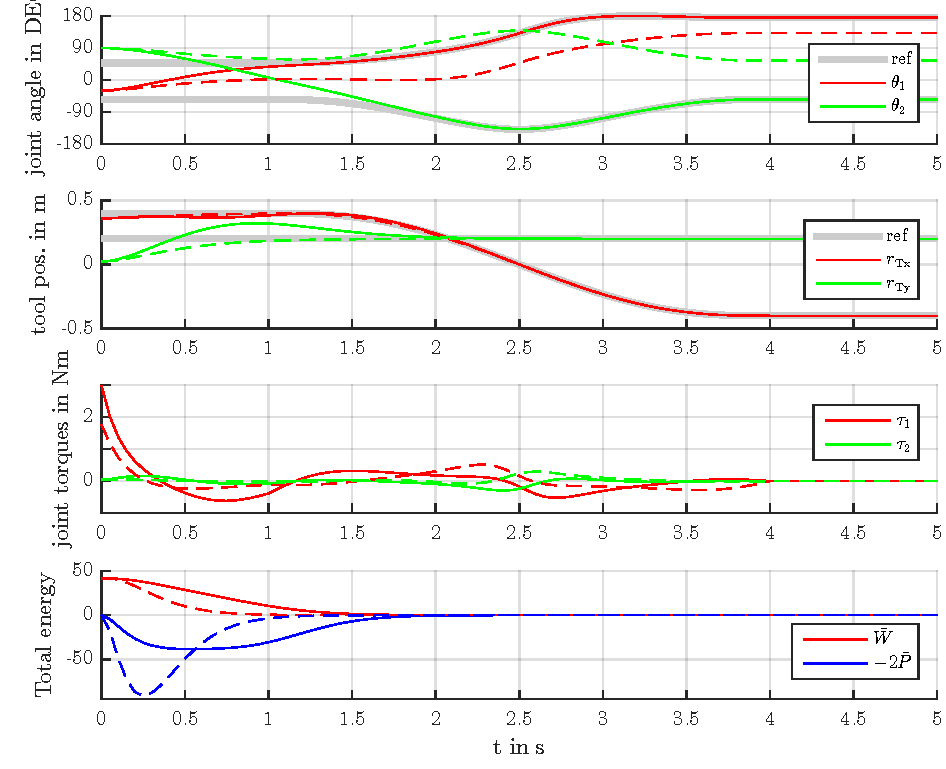
\includegraphics[]{SCARA/ScaraSimRes.pdf}
 \caption{Simulation result for the SCARA with parameterization 1 (solid lines) and 2 (dashed lines)}
 \label{fig:ScaraSimRes}
\end{figure}

\begin{figure}[htb]
 \centering
 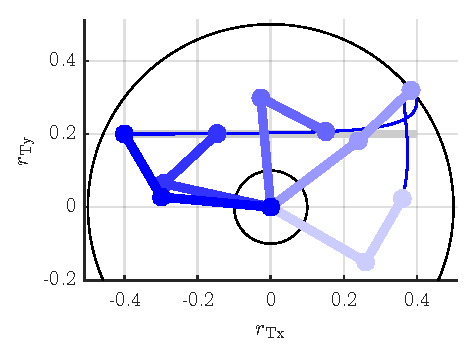
\includegraphics[]{SCARA/ScaraSnapApproach1.pdf}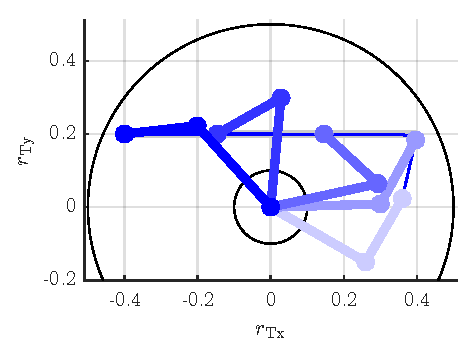
\includegraphics[]{SCARA/ScaraSnapApproach2.pdf}
 \caption{Snapshots for the simulation result for the SCARA with parameterization 1 (left) and 2 (right)}
 \label{fig:ScaraSimSnapshots}
\end{figure}

\begin{figure}[ht]
 \centering
 \input{graphics/SCARAPotential.pdf_tex}
 \caption{
 The controlled potential energy $\potentialEnergy$ for parameterization 1 (left) and 2 (right) for $\jointAngleR[1] = 0$, $\jointAngleR[2] = \tfrac{\pi}{2}$. %on the half open set $\jointAngle[1], \jointAngle[2] = (-\pi,\pi]$.
 Blue dots are minima, red are maxima and green are saddle points.
 }
 \label{fig:SCARAPotentials}
\end{figure}



\clearpage
\subsection{Robot arm}
As a more complex multibody system we consider a robot arm as illustrated in \autoref{fig:RobotArmModel}.
For this example the model equations and the resulting closed loop equations become quite cumbersome and are not displayed explicitly.
However this displays some benefits of the proposed control approach: One does not have to look at e.g.\ the actual system inertia matrix but only at the much less cumbersome body inertia matrices to conclude e.g.\ stability of the closed loop. 

\paragraph{Model.}
\begin{figure}[ht]
 \centering
 \input{graphics/KukaRobotModel.pdf_tex}
 \caption{A model of a robot arm (background image from www.kuka.de)}
 \label{fig:RobotArmModel}
\end{figure}
A reasonable choice of coordinates of the system are the joint angles $\sysCoord = [\jointAngle[1], \ldots, \jointAngle[6]]^\top$ and trivial kinematics $\sysVel = \sysCoordd$.
The body configurations can be computed from the following relative transformations
\begin{align}
 \bodyHomoCoord{0}{1}{}{} &=
 \begin{bmatrix}
  \cos\jointAngle[1] & -\sin\jointAngle[1] & 0 & 0 \\
  \sin\jointAngle[1] &  \cos\jointAngle[1] & 0 & 0 \\
  0 & 0 & 1 & 0 \\
  0 & 0 & 0 & 1
 \end{bmatrix},&
 \bodyHomoCoord{1}{2}{}{} &=
 \begin{bmatrix}
  \cos\jointAngle[2] & 0 & \sin\jointAngle[2] & l_1 \\
  0 & 1 & 0 & 0 \\
  -\sin\jointAngle[2] & 0 & \cos\jointAngle[2] & 0 \\
  0 & 0 & 0 & 1
 \end{bmatrix},
\nonumber\\
 \bodyHomoCoord{2}{3}{}{} &=
 \begin{bmatrix}
  \cos\jointAngle[3] & 0 & \sin\jointAngle[3] & 0 \\
  0 & 1 & 0 & 0 \\
  -\sin\jointAngle[3] & 0 & \cos\jointAngle[3] & l_2 \\
  0 & 0 & 0 & 1
 \end{bmatrix},&
 \bodyHomoCoord{3}{4}{}{} &=
 \begin{bmatrix}
  1 & 0 & 0 & l_3 \\
  0 & \cos\jointAngle[4] & -\sin\jointAngle[4] & 0 \\
  0 & \sin\jointAngle[4] &  \cos\jointAngle[4] & 0 \\
  0 & 0 & 0 & 1
 \end{bmatrix},
\nonumber\\
 \bodyHomoCoord{4}{5}{}{} &=
 \begin{bmatrix}
  \cos\jointAngle[5] & 0 & \sin\jointAngle[5] & 0 \\
  0 & 1 & 0 & 0 \\
  -\sin\jointAngle[5] & 0 & \cos\jointAngle[5] & 0 \\
  0 & 0 & 0 & 1
 \end{bmatrix},&
 \bodyHomoCoord{5}{6}{}{} &=
 \begin{bmatrix}
  1 & 0 & 0 & 0 \\
  0 & \cos\jointAngle[6] & -\sin\jointAngle[6] & 0 \\
  0 & \sin\jointAngle[6] &  \cos\jointAngle[6] & 0 \\
  0 & 0 & 0 & 1
 \end{bmatrix}
 .
\end{align}
This together with the body inertia matrices and the gravity coefficients $\gravityAcc$ and the control forces, $\sysInput = [\tau_1, \ldots, \tau_6]^\top$ determines the equations of motion.

\paragraph{Controller parameterization 1: Joint space control.}
Like above we consider two different sets of controller parameterizations: 
For the first case, the nonzero control parameters are
\begin{align}
 \bodyMOSCoeffC{0}{1}{\idxZ\idxZ}, \bodyMOSCoeffC{1}{2}{\idxY\idxY}, \bodyMOSCoeffC{2}{3}{\idxY\idxY}, \bodyMOSCoeffC{3}{4}{\idxX\idxX}, \bodyMOSCoeffC{4}{5}{\idxY\idxY}, \bodyMOSCoeffC{5}{6}{\idxX\idxX} &\in \RealNum > 0
\nonumber\\
 \bodyMODCoeffC{0}{1}{\idxZ\idxZ}, \bodyMODCoeffC{1}{2}{\idxY\idxY}, \bodyMODCoeffC{2}{3}{\idxY\idxY}, \bodyMODCoeffC{3}{4}{\idxX\idxX}, \bodyMODCoeffC{4}{5}{\idxY\idxY}, \bodyMODCoeffC{5}{6}{\idxX\idxX} &\in \RealNum > 0
\nonumber\\
 \bodyMOICoeffC{0}{1}{\idxZ\idxZ}, \bodyMOICoeffC{1}{2}{\idxY\idxY}, \bodyMOICoeffC{2}{3}{\idxY\idxY}, \bodyMOICoeffC{3}{4}{\idxX\idxX}, \bodyMOICoeffC{4}{5}{\idxY\idxY}, \bodyMOICoeffC{5}{6}{\idxX\idxX} &\in \RealNum > 0
\end{align}
A transport map for the resulting potential energy is $\sysTransportMap = \idMat[6]$.
The resulting closed loop kinetics are 6 decoupled equations identical to the ones for the SCARA \eqref{eq:ScaraClosedLoop11} resp.\ \eqref{eq:ScaraClosedLoop12}.

\paragraph{Controller parameterization 2: Work space control.}
As a second case consider: For many applications the task of the robot arm is to control the position and orientation of a tool mounted at the end of its kinematic chain.
This tool might have a particularly meaningful center point (TCP) and and principle axes.
Let the configuration $\bodyHomoCoord{6}{7} = \const$ capture these tool specific parameters, for example the tip position and direction of a welding electrode as shown in \autoref{fig:WeldingTool}.

\begin{figure}[ht]
 \centering
 \input{graphics/WeldingTool.pdf_tex}
 \caption{Welding tool attached to the robot arm (background image from www.kuka.de)}
 \label{fig:WeldingTool}
\end{figure}

For this example it could be useful to control the tool as if it is a free rigid body (with its center of mass, damping and stiffness at the TCP) and not care about the particular mechanism that is used to give it this degree of freedom.
This is achieved by the following nonzero control parameters
\begin{align}
 \bodyStiffnessC{0}{7}, \bodyDampingC{0}{7}, \bodyMassC{0}{7} \in \RealNumP,
\qquad
 \bodyMOSC{0}{7}, \bodyMODC{0}{7}, \bodyMOIC{0}{7} \in \SymMatP(3).
%\qquad
% \bodyCOSC{0}{7}, \bodyCODC{0}{7}, \bodyCOMC{0}{7} = \tuple{0}.
\end{align}
The resulting potential and corresponding transport map are
\begin{align}
 \potentialEnergyC(\sysCoord, \sysCoordR) = \tfrac{1}{2} \norm[\bodyStiffMatCp{0}{7}]{ ((\bodyHomoCoord{0}{7}(\sysCoordR))^{-1}\, \bodyHomoCoord{0}{7}(\sysCoord) - \idMat[4] )^\top}^2,
\quad
 \sysTransportMap(\sysCoord,\sysCoordR) = \big( \bodyJac{7}{0}(\sysCoord) \big)^{-1} \, \bodyJac{7}{0}(\sysCoordR).
\end{align}
% A transport map for the resulting potential is
% \begin{align}
%  \sysTransportMap(\sysCoord,\sysCoordR)
% % = \big( \bodyJac{0}{7}(\sysCoord) \big)^{-1} \Ad{(\bodyHomoCoord{0}{7}(\sysCoord))^{-1} \bodyHomoCoord{0}{7}(\sysCoordR)} \bodyJac{0}{7}(\sysCoordR)
%  = \big( \bodyJac{7}{0}(\sysCoord) \big)^{-1} \, \bodyJac{7}{0}(\sysCoordR)
% \end{align}
The resulting closed loop dynamics of the robot arm may be written by plugging the absolute tool configuration $\bodyHomoCoord{0}{7}(\sysCoord)$ and its reference $\bodyHomoCoord{0}{7}(\sysCoordR)$ into the dynamics of a single rigid body for either of the three proposed approaches \eqref{eq:RBCtrlParticles}, \eqref{eq:RBCtrlBody} or \eqref{eq:RBCtrlEnergy}.

The determinant of the transport map is
\begin{align}
 \det \sysTransportMap(\sysCoord,\sysCoordR) = \frac{\det \bodyJac{0}{7}(\sysCoordR)}{\det \bodyJac{0}{7}(\sysCoord)},
\quad
 \det \bodyJac{0}{7}(\sysCoord) = -l_2 l_3 (l_1 + l_2 \sin\jointAngle[2] + l_3 \cos(\jointAngle[2]+\jointAngle[3])) \cos\jointAngle[3] \sin\jointAngle[5]
\end{align}
If the term in the brackets vanishes means that the wrist lies on the axis of $\jointAngle[1]$ and $\cos\jointAngle[3] = 0$ is the case if the arm is completely straight which is the singularity we already encountered with the SCARA robot.
The last three axis with angles $\jointAngle[4]$, $\jointAngle[5]$, $\jointAngle[6]$ can be regarded as Euler angles in the sequence XYX and $\sin\jointAngle[5] = 0$ is their singularity.
Comparing this to the motivation example in \autoref{sec:MotivationRigidBodyAttitude} we have the same problem but the other way around:
The Euler angles are an absolutely appropriate choice of coordinates since the mechanism is realized like this.
Consequently the configuration manifold of this part is $\Sphere^1 \times \Sphere^1 \times \Sphere^1$ and we are assigning a control that was designed for $\SpecialOrthogonalGroup(3)$.

\paragraph*{Conclusion.}
The behavior of the two different parameterizations are quite analog to the two parameterizations of the SCARA robot.
Which one is more suitable depends on the actual control task.
Furthermore, the two presented parameterizations are just two special cases of which dynamics can be achieved with the more general approach of control of this work. 


\clearpage
\section{Examples of underactuated systems}
\subsection{Two masses connected by a spring}
In order to illustrate the control approach for underactuated systems we consider the minimal example:
Two bodies in prismatic joints connected by a linear spring but where only one is directly actuated by the force $F$ as illustrated in \autoref{fig:TwoMassSpring}.
\begin{figure}[ht]
 \centering
 \input{graphics/TwoMassSpring.pdf_tex}
 \caption{Model of two bodies connected by a spring}
 \label{fig:TwoMassSpring}
\end{figure}

\paragraph{Model.}
We choose the absolute positions of the bodies as configuration coordinates $\sysCoord = [z_1, z_2]^\top$ and their derivative as velocity coordinates $\sysVel = \sysCoordd$.
With this the body configurations are
\begin{align}
 \bodyHomoCoord{0}{1} = \begin{bmatrix} 1 & 0 & 0 & z_1 \\ 0 & 1 & 0 & 0 \\ 0 & 0 & 1 & 0 \\ 0 & 0 & 0 & 1\end{bmatrix},
\qquad
 \bodyHomoCoord{0}{2} = \begin{bmatrix} 1 & 0 & 0 & z_2 \\ 0 & 1 & 0 & 0 \\ 0 & 0 & 1 & 0 \\ 0 & 0 & 0 & 1\end{bmatrix}.
\end{align}
With the total mass $\bodyMass{0}{1}$, $\bodyMass{0}{2}$ of the individual bodies and the spring stiffness $\bodyStiffness{1}{2}$ the resulting equations of motion may be written as
\begin{align}\label{eq:TwoMassSpringModel}
 \underbrace{\begin{bmatrix} \bodyMass{0}{1} & 0 \\ 0 & \bodyMass{0}{2} \end{bmatrix}}_{\sysInertiaMat}
 \begin{bmatrix} \ddot{z}_1 \\ \ddot{z}_2 \end{bmatrix}
 +
 \underbrace{\begin{bmatrix} \bodyStiffness{1}{2} & -\bodyStiffness{1}{2} \\ -\bodyStiffness{1}{2} & \bodyStiffness{1}{2} \end{bmatrix}}_{\sysStiffMat}
 \begin{bmatrix} z_1 \\ z_2 \end{bmatrix} 
 =
 \underbrace{\begin{bmatrix} 1 \\ 0 \end{bmatrix}}_{\sysInputMat} F
 .
\end{align}
% Obviously the second equation is independent of the control force $\sysInput = F$:
% \begin{align}\label{eq:accConstTwoMassSpring}
%  \sysInputMatLComp = [0 \ 1], \qquad \sysInputMatLComp (\sysInertiaMat \sysVeld + \d_{\sysVel} \potentialEnergy) &= 0&
% &\Rightarrow&
%  \ddot{z}_2 + \underbrace{\tfrac{\bodyStiffness{1}{2}}{\bodyMass{0}{2}}}_{\varpi} (z_2 - z_1) &= 0
%  .
% \end{align}
% From this its obvious that $z_2$ is a \textit{flat output} of the system and we can utilize this to compute suitable reference trajectories $t \mapsto (\sysCoord[1](t), \sysCoord[2](t))$ which obey the EOM.

\paragraph{Desired closed loop.}
We assume general body inertia $\bodyInertiaMat{0}{1},\ldots$, damping and stiffness.
The three proposed control approaches lead to identical desired closed loop dynamics:
\begin{align}\label{eq:TwoMassSpringClosedLoop}
 \sysInertiaMatC \sysCoordEdd + \sysDissMatC \sysCoordEd + \sysStiffMatC \sysCoordE = \tuple{0},
\qquad
 \sysCoordE = \sysCoord - \sysCoordR
\end{align}
where
\begin{align}
 \sysInertiaMatC &= \begin{bmatrix} \bodyMassC{0}{1} + \bodyMassC{1}{2} & -\bodyMassC{1}{2} \\ -\bodyMassC{1}{2} & \bodyMassC{0}{2}+\bodyMassC{1}{2} \end{bmatrix},&
 \sysDissMatC &= \begin{bmatrix} \bodyDampingC{0}{1} + \bodyDampingC{1}{2} & -\bodyDampingC{1}{2} \\ -\bodyDampingC{1}{2} & \bodyDampingC{0}{2}+\bodyDampingC{1}{2} \end{bmatrix},&
 \sysStiffMatC &= \begin{bmatrix} \bodyStiffnessC{0}{1} + \bodyStiffnessC{1}{2} & -\bodyStiffnessC{1}{2} \\ -\bodyStiffnessC{1}{2} & \bodyStiffnessC{0}{2}+\bodyStiffnessC{1}{2} \end{bmatrix}.
\end{align}
The corresponding potential $\potentialEnergyC = \tfrac{1}{2} \sysCoordE^\top \sysStiffMatC \sysCoordE$ has the obvious transport map $\sysTransportMap = \idMat[2]$.


\paragraph{Matching.}
The matching condition \eqref{eq:MatchingCondition} for this example may be written as
\begin{align}
 \tuple{\lambda} = (\sysInputMatLComp)^\top (\sysInertiaMat \sysInertiaMatC^{-1} (-\sysInertiaMatC \sysCoordRdd + \sysDissMatC (\sysCoordd-\sysCoordRd) + \sysStiffMatC (\sysCoord-\sysCoordR)) - \sysStiffMat \sysCoord) &= \tuple{0}.
\end{align}
Since this equation is linear in the system coordinates we can separate the into
\begin{subequations}
\begin{align}
 (\sysInputMatLComp)^\top (\sysInertiaMat \sysCoordRdd + \sysStiffMat \sysCoordR) &= \tuple{0}.
\\
 (\sysInputMatLComp)^\top \sysInertiaMat \sysInertiaMatC^{-1} \sysDissMatC &= \mat{0},
\\
 (\sysInputMatLComp)^\top \sysInertiaMat \sysInertiaMatC^{-1} (\sysStiffMatC - \sysStiffMat) &= \mat{0},
\end{align}
\end{subequations}
Choosing $\sysInputMatLComp = [0, 1]^\top$ this is explicitly
\begin{subequations}
\begin{align}
 &\ddot{z}_{2\idxRef} + \varpi (z_{2\idxRef} - z_{1\idxRef}) = 0
 \label{eq:TwoMassSpringFlatnessCondition}
\\
 &\left\{ \begin{matrix}
  \bodyMassC{0}{1} \bodyDampingC{1}{2} - \bodyMassC{1}{2} \bodyDampingC{0}{1} = 0 \\
  \bodyMassC{0}{1} \bodyDampingC{1}{2} + (\bodyMassC{0}{1} + \bodyMassC{1}{2}) \bodyDampingC{0}{2} = 0
 \end{matrix} \right.
\\
 &\left\{ \begin{matrix}
  \bodyMassC{0}{1} \bodyStiffnessC{1}{2} - \bodyMassC{1}{2} \bodyStiffnessC{0}{1} = (\bodyMassC{0}{1} \bodyMassC{0}{2}+\bodyMassC{0}{1} \bodyMassC{1}{2}+\bodyMassC{0}{2} \bodyMassC{1}{2}) \varpi \\
 \bodyMassC{0}{1} \bodyStiffnessC{1}{2} + (\bodyMassC{0}{1} + \bodyMassC{1}{2}) \bodyStiffnessC{0}{2} = (\bodyMassC{0}{1} \bodyMassC{0}{2}+\bodyMassC{0}{1} \bodyMassC{1}{2}+\bodyMassC{0}{2} \bodyMassC{1}{2}) \varpi
 \end{matrix} \right.
\end{align}
\end{subequations}
where $\varpi = \sfrac{\bodyStiffness{1}{2}}{\bodyMass{0}{2}}$ is the sole model parameter relevant for the matching condition.
The first part \eqref{eq:TwoMassSpringFlatnessCondition} is a constraint on the reference trajectory as it is independent of tunable parameters.
It can be resolved by acknowledging that $z_2$ is a \textit{flat output} of the system and planing the reference trajectory accordingly, i.e.
\begin{align}
 z_{1\idxRef} = z_{2\idxRef} - \sfrac{\ddot{z}_{2\idxRef}}{\varpi}. 
\end{align}
The other conditions can be resolved by setting
\begin{align}\label{eq:TwoMassSpringMatchingConditionSolution}
 \bodyStiffnessC{1}{2} &=  \tfrac{\bodyMassC{1}{2}}{\bodyMassC{0}{1}} \bodyStiffnessC{0}{1} + \tfrac{\bodyMassC{0}{1} \bodyMassC{0}{2} + \bodyMassC{0}{1} \bodyMassC{1}{2} + \bodyMassC{0}{2} \bodyMassC{1}{2}}{\bodyMassC{0}{1}} \varpi,&
 \bodyStiffnessC{0}{2} &= -\tfrac{\bodyMassC{1}{2}}{\bodyMassC{0}{1}+\bodyMassC{1}{2}} \bodyStiffnessC{0}{1},&
 \bodyDampingC{1}{2} &= \tfrac{\bodyMassC{1}{2}}{\bodyMassC{0}{1}} \bodyDampingC{0}{1},&
 \bodyDampingC{0}{2} &= -\tfrac{\bodyMassC{1}{2}}{\bodyMassC{0}{1}+\bodyMassC{1}{2}} \bodyDampingC{0}{1},
\end{align}
which leaves the 5 tuning parameters $\bodyStiffnessC{0}{1}$, $\bodyDampingC{0}{1}$, $\bodyMassC{0}{1}$, $\bodyMassC{0}{2}$ and $\bodyMassC{1}{2}$.

The resulting control law is
\begin{multline}
 F = \bodyMass{0}{1} \ddot{z}_{1\idxRef}  +  \bodyStiffness{1}{2} (z_{1\idxRef} - z_{2\idxRef})
 + \big( \bodyStiffness{1}{2} + \tfrac{\bodyMass{0}{1} (\bodyMassC{1}{2} \bodyStiffness{1}{2} + \bodyMass{0}{2} (\bodyStiffnessC{0}{1} - \bodyStiffnessC{1}{2}))}{\bodyMass{0}{2} (\bodyMassC{0}{1} + \bodyMassC{1}{2})} \big) e_1
\\
 - \big( \bodyStiffness{1}{2} - \tfrac{\bodyMass{0}{1} (\bodyMassC{1}{2} \bodyStiffness{1}{2} - \bodyMass{0}{2} \bodyStiffnessC{1}{2})}{\bodyMass{0}{2} (\bodyMassC{0}{1} + \bodyMassC{1}{2})} \big) e_2
 - \tfrac{\bodyMass{0}{1} (\bodyDampingC{0}{1} + \bodyDampingC{1}{2})}{\bodyMassC{0}{1} + \bodyMassC{1}{2}} \dot{e}_1
 + \tfrac{\bodyMass{0}{1} \bodyDampingC{1}{2}}{\bodyMassC{0}{1} + \bodyMassC{1}{2}} \dot{e}_2
 .
\end{multline}

\paragraph{Pole placement.}
Tuning the design parameters under the given matching conditions might not be intuitive for this example.
To resolve this we can fall back to the classical approach of placing the eigenvalues of the closed loop system \eqref{eq:TwoMassSpringClosedLoop}.
Taking into account the matching condition \eqref{eq:TwoMassSpringMatchingConditionSolution}, the characteristic polynomial of \eqref{eq:TwoMassSpringClosedLoop} is
\begin{align}
 \tfrac{\det (\sysInertiaMatC \EigenVal^2 + \sysDissMatC \EigenVal + \sysStiffMatC)}{\det \sysInertiaMatC}
 =
 \EigenVal^4 
 + \underbrace{\tfrac{\bodyDampingC{0}{1}}{\bodyMassC{0}{1}}}_{p_3} \EigenVal^3
 + \underbrace{\tfrac{\bodyStiffnessC{0}{1} + (\bodyMassC{0}{1}+\bodyMassC{0}{2})\varpi}{\bodyMassC{0}{1}}}_{p_2} \EigenVal^2
 + \underbrace{\tfrac{\varpi \bodyDampingC{0}{1}}{\bodyMassC{0}{1}+\bodyMassC{1}{2}}}_{p_1} \EigenVal
 + \underbrace{\tfrac{\varpi \bodyStiffnessC{0}{1}}{\bodyMassC{0}{1}+\bodyMassC{1}{2}}}_{p_0}
 .
\end{align}
This can be solved for
\begin{subequations}
\begin{align}
 \bodyStiffnessC{0}{1}  &= \tfrac{\bodyMassC{1}{2} p_0 p_3}{\varpi p_3 - p_1},&
 \bodyDampingC{0}{1}    &= \tfrac{\bodyMassC{1}{2} p_1 p_3}{\varpi p_3 - p_1},&
 \bodyMassC{0}{1}       &= \tfrac{\bodyMassC{1}{2} p_1}{\varpi p_3 - p_1},&
 \bodyMassC{0}{2}       &= \tfrac{\bodyMassC{1}{2} (p_1 p_2 - p_0 p_3 - \varpi p_1)}{\varpi(\varpi p_3 - p_1)}
 .
\end{align}
\end{subequations}
and $\bodyMassC{1}{2} \in \RealNum \neq 0$.
Choosing any Hurwitz polynomial for the coefficients $p_i$ guarantees the asymptotic stability of the closed loop.
In order to conclude $\sysInertiaMatC > 0$, $\sysDissMatC \geq 0$ and $\sysStiffMatC > 0$ from the Hurwitz criterion ($p_0, p_1, p_2, p_3, p_1 p_2 - p_0 p_3, p_1 p_2 p_3 - p_1^2 - p_0 p_3^2 > 0$) we need $\sign \bodyMassC{1}{2} = \sign (\varpi p_3 - p_1)$.

\paragraph{Conclusions.}
The resulting controller is equivalent to one that could be designed by standard linear state-feedback methods.
However, this approach here might give some \textit{physical} insight to the resulting closed loop system.
For example that the closed loop system must have an inertial coupling ($\bodyMassC{1}{2} \neq 0$) of the two bodies, if one wants to tune all 4 poles.

\subsection{PVTOL}
The planar vertical take off landing aircraft (PVTOL) as depicted in \autoref{fig:PVTOLModel}, is a common benchmark problem discussed in e.g.\ \cite{Hauser:PVTOL} or \cite{Fliess:LieBacklund}.
\begin{figure}
 \centering
% \def\svgwidth{.5\textwidth}
 \input{graphics/PVTOLModel.pdf_tex}
 \caption{Model of the PVTOL}
 \label{fig:PVTOLModel}
\end{figure}

\paragraph{Model.}
The model of the PVTOL is a planar rigid body alredy discussed in \autoref{sec:CtrlPlanarRigidBody} supplemented with gravity and the specific actuation $F_\text{r}$, $F_\text{l}$ depicted in \autoref{fig:PVTOLModel}.
Here, we chose the body fixed frame to be positioned at the center of mass, i.e.\ $\sx = \sy = 0$.
The kinetic equation takes the form
\begin{align}
 \underbrace{\begin{bmatrix} \m & 0 & 0 \\ 0 & \m & 0 \\ 0 & 0 & \Jz \end{bmatrix}}_{\sysInertiaMat}
 \underbrace{\begin{bmatrix} \vxd \\ \vyd \\ \wzd \end{bmatrix}}_{\sysVeld}
 +
%  \underbrace{\begin{bmatrix} -m \vy \wz \\ m \vx \wz \\ 0 \end{bmatrix}}_{\gyroForce}
%  +
%  \underbrace{\begin{bmatrix} m \gravityAccConst \sin\tiltAngle \\ m \gravityAccConst \cos\tiltAngle \\ 0 \end{bmatrix}}_{\differential \potentialEnergy}
 \underbrace{\begin{bmatrix} m(\gravityAccConst \sin\tiltAngle - \vy \wz) \\ m (\gravityAccConst \cos\tiltAngle + \vx \wz) \\ 0 \end{bmatrix}}_{\sysForce}
 =
 \underbrace{\begin{bmatrix} \sin\beta & -\sin\beta \\ \cos\beta & \cos\beta \\ \ArmRadius \cos\beta & -\ArmRadius\cos\beta \end{bmatrix}}_{\sysInputMat}
 \underbrace{\begin{bmatrix} F_\text{r} \\ F_\text{l} \end{bmatrix}}_{\sysInput}
 .
\end{align}
% \fixme{Input trafo}
% \begin{align}
% %  F_m &= \cos\beta (F_\text{r} + F_\text{l}),
% %  \tau = a \cos\beta (F_\text{r} - F_\text{l})
% % \qquad \Leftrightarrow \qquad
% %  F_\text{r} = \tfrac{1}{2 \cos\beta} (F_m + \tfrac{\tau}{a}), \
% %  F_\text{l} = \tfrac{1}{2 \cos\beta} (F_m - \tfrac{\tau}{a})
%  \begin{bmatrix} F_m \\ \tau \end{bmatrix}
%  = \begin{bmatrix} \cos\beta & \cos\beta \\ a \cos\beta & -a \cos\beta \end{bmatrix}
%  \begin{bmatrix} F_\text{r} \\ F_\text{l} \end{bmatrix}
% \end{align}

\paragraph{Reference trajectory.}
For the following we chose $\sysInputMatLComp = [1, 0, -\tfrac{\sin\beta}{l \cos\beta}]$ as a left complement to $\sysInputMat$.
With this, the matiching condition for the reference from \eqref{eq:MatchingForceZeroError} reads
\begin{align}
 \lambda^{\text{ZeroError}} = \m \big(\vRxd - \underbrace{\tfrac{\Jz \sin\beta}{\m \ArmRadius \cos\beta}}_{\eps} \wRzd - \wRz \vRy + \gravityAccConst \sin\tiltAngleR \big) = 0
\end{align}
This can be fulfilled by parameterizing the configuration through the flat output $y_{1\idxRef} = \rRx - \eps \sin\tiltAngleR$, $y_{2\idxRef} = \rRy + \eps \cos\tiltAngleR$ (see e.g.\ \cite{Fliess:LieBacklund}), i.e.
\begin{align}
 \rxR &= y_{1\idxRef} - \eps \frac{\ddot{y}_{1\idxRef}}{\sqrt{\ddot{y}_{1\idxRef}^2 + (\ddot{y}_{2\idxRef}+\gravityAccConst)^2}},
\\
 \ryR &= y_{2\idxRef} - \eps \frac{\ddot{y}_{2\idxRef}-\gravityAccConst}{\sqrt{\ddot{y}_{1\idxRef}^2 + (\ddot{y}_{2\idxRef}+\gravityAccConst)^2}},
\\
 \tiltAngle_{\idxRef} &= \atanTwo(\ddot{y}_{1\idxRef}, \ddot{y}_{2\idxRef}+\gravityAccConst).
\end{align}
Note that this parameterization fails if $\ddot{y}_{1\idxRef} = \ddot{y}_{2\idxRef}+\gravityAccConst = 0$, i.e. the body is in free fall.

% \begin{align}
%  \matchingForceR = \m (\ddot{y}_{1\idxRef} \cos\tiltAngleR + (\ddot{y}_{2\idxRef} + \gravityAccConst) \sin\tiltAngleR) = 0
% \end{align}

\paragraph{Closed loop.}
As for the model, the closed loop templates are the ones the planar rigid body from \autoref{sec:CtrlPlanarRigidBody}. 
Due to symmetry reasons we set the parameters $\hcx=\lcx=\scx=0$.
% \begin{align}
%  \potentialEnergyC &= \tfrac{1}{2} \kc \big( (\rEx - \hcy \sin\tiltAngleE)^2 + (\rEy + \hcy(\cos\tiltAngleE-1))^2 \big) + \kapcz (1-\cos\tiltAngleE),
% \\
%  \sysDissMatC &= \begin{bmatrix} \dc & 0 & -\dc \lcy \\ 0 & \dc & 0 \\ -\dc \lcy & 0 & \sigcz + \dc \lcy^2 \end{bmatrix},
%  \qquad
%  \sysInertiaMatC = \begin{bmatrix} \mc & 0 & -\mc \scy \\ 0 & \mc & 0 \\ -\mc \scy & 0 & \Jcz + \mc \scy^2 \end{bmatrix}
% \end{align}
% This leads to the desired closed loop kinetics
% \begin{multline}
%  \underbrace{\begin{bmatrix} \mc & 0 & -\mc \scy \\ 0 & \mc & 0 \\ -\mc \scy & 0 & \Jcz + \mc \scy^2 \end{bmatrix}}_{\sysInertiaMatC}
%  \underbrace{\begin{bmatrix} \vExd \\ \vEyd \\ \wEzd \end{bmatrix}}_{\sysVelEd}
%  +
%  \underbrace{\begin{bmatrix} -\mc \wz \vEy \\ \mc \wz (\vEx - \scy \wEz) \\ \mc \scy \wz \vEy \end{bmatrix}}_{\gyroForceC}
% \\
%  +
%  \underbrace{\begin{bmatrix} \dc & 0 & -\dc \lcy \\ 0 & \dc & 0 \\ -\dc \lcy & 0 & \sigcz + \dc \lcy^2 \end{bmatrix}}_{\sysDissMatC}
%  \underbrace{\begin{bmatrix} \vEx \\ \vEy \\ \wEz \end{bmatrix}}_{\sysVelE}
%  +
%  \underbrace{\begin{bmatrix} \kc (\hcy \sin\tiltAngleE - \rEx) \\ \kc (\hcy (1-\cos\tiltAngleE) - \rEy) \\ \kc \hcy (\rEx - \hcy \sin\tiltAngleE) - \kapcz \sin\tiltAngleE \end{bmatrix}}_{\differential \potentialEnergyC}
%  =
%  \tuple{0}.
% \end{multline}

\paragraph{Matching.}
The matching force $\tuple{\lambda}$ from \eqref{eq:DefMatchingForce} with the orthogonal complement from above takes a rather cumbersome form and is not given explicitly here.
Instead we will investigate its linear approximation about any reference trajectory with $\tiltAngle_\idxRef = 0$: The matrices of the linearized model and desired closed loop are
\begin{subequations}
\begin{align}
 \sysInertiaMatLin &= \begin{bmatrix} m & 0 & 0 \\ 0 & m & 0 \\ 0 & 0 & J \end{bmatrix},&
 \sysInertiaMatCLin &= \begin{bmatrix} \mc & 0 & -\mc\scy \\ 0 & \mc & 0 \\ -\mc\scy & 0 & \Jcz + \mc\scy^2 \end{bmatrix},
\\
 \sysDissMatLin &= \begin{bmatrix} 0 & 0 & 0 \\ 0 & 0 & 0 \\ 0 & 0 & 0 \end{bmatrix},&
 \sysDissMatCLin &= \begin{bmatrix} \dc & 0 & -\dc\lcy \\ 0 & \dc & 0 \\ -\dc\lcy & 0 & \sigcz + \dc\lcy^2 \end{bmatrix},
\\
 \sysStiffMatLin &= \begin{bmatrix} 0 & 0 & m \gravityAccConst \\ 0 & 0 & 0 \\ 0 & 0 & 0 \end{bmatrix},&
 \sysStiffMatCLin &= \begin{bmatrix} \kc & 0 & -\kc\hcy \\ 0 & \kc & 0 \\ -\kc\hcy & 0 & \kapcz + \kc\hcy^2 \end{bmatrix}.
\end{align}
\end{subequations}
The conditions for $(\sysInputMatLComp)^\top \big( \sysInertiaMatLin \sysInertiaMatCLin^{-1} \sysDissMatCLin - \sysDissMatLin\big) = \mat{0}$ and $(\sysInputMatLComp)^\top \big( \sysInertiaMatLin \sysInertiaMatCLin^{-1} \sysStiffMatCLin - \sysStiffMatLin\big) = \mat{0}$ for the linearized matching force from \eqref{eq:MatchingForceLin} to vanish are equivalent to
\begin{subequations}\label{eq:PVTOLMatchingCondLin}
\begin{align}
 \kc \big( \Jcz - \mc(\hcy - \scy)(\scy - \eps) \big) &= 0,
\\
 \mc \kapcz (\scy-\eps) - \kc\hcy \big( \Jcz - \mc (\hcy - \scy)(\scy - \eps) \big) &= \Jcz \mc \gravityAccConst, 
\\
 \dc \big( \Jcz - \mc(\lcy - \scy)(\scy - \eps) \big) &= 0,
\\
 \mc \sigcz (\scy-\eps) - \dc\,\lcy \big( \Jcz - \mc (\lcy - \scy)(\scy - \eps) \big) &= 0.
\end{align}
\end{subequations}
One solution for this is
\begin{align}\label{eq:PVTOLMatchingSolution}
 \Jcz &= \mc(\hcy - \scy)(\scy - \eps),&
 \lcy &= \hcy,&
 \sigcz &= 0,&
 \kapcz &= \mc \gravityAccConst (\hcy-\scy)
\end{align}
which leaves the parameters $\kc, \dc, \mc, \hcy, \scy$ for tuning.
For the energies to be positive (semi) definite, i.e.\ $\sysInertiaMatC > 0$, $\sysDissMatC \geq 0$ and $\potentialEnergyC > 0$ we need
\begin{align}
 \kc, \dc, \mc > 0, \qquad \hcy > \scy > \eps.
\end{align}

The remaining matching force is
\begin{align}
 \tilde{\sysForce} = \frac{\mc(\hcy-\scy)}{m(\hcy-\eps)} \begin{bmatrix} 1 \\ 0 \\ -\eps \end{bmatrix} \lambda
\end{align}
where $\lambda$ for the corresponding approach is
\begin{subequations}
\begin{align}
 \lambda^{\text{ParticleBased}} &= m(a_{\idxY\idxRef} - \eps\wzR^2)\sin\tiltAngleE
\\
 \lambda^{\text{BodyBased}} &= m(a_{\idxY\idxRef}\sin\tiltAngleE - \rxE\wzR^2 + 2\vyE\wzR + (\eps(1-\cos\tiltAngleE)-\ryE)\wzRd)
\\
 \lambda^{\text{EnergyBased}} &= m(a_{\idxY\idxRef}\sin\tiltAngleE - \rxE\wzR^2 +\phantom{2}\vyE\wzR + (\eps(1-\cos\tiltAngleE)-\ryE)\wzRd)
\end{align} 
\end{subequations}
where $a_{\idxY\idxRef} = \vyRd + \vxR\wzR + \gravityAccConst(\cos\tiltAngleR - 1)$. 
Note that for a constant reference motion $\vRd = 0$ (which implies $\tiltAngleR = 0$) the matching force vanishes $\lambda = 0$ for all approaches.


\begin{figure}
 \centering
 \input{graphics/PVTOLPendulum2.pdf_tex}
 \caption{Interpretation of the controlled PVTOL as a mechanical system} 
 \label{fig:PVTOLPendulum}
\end{figure}

\paragraph{Mechanical interpretation.}
The closed loop template is a planar rigid body with attached springs and dampers as motivated in \autoref{sec:RB} but without gravity.
Taking into account the parameter constraints \eqref{eq:PVTOLMatchingSolution}, the controlled PVTOL corresponds to the mechanical system illustrated in \autoref{fig:PVTOLPendulum}.
The condition $\hcy > \scy$ implies that the center of mass must be below the center of stiffness.
As dicussed in \autoref{sec:DecouplingRigidBody}, $\hcy \neq \scy$ results in a coupling between translational and rotational motion.
From a stability/attractiveness point of view this is necessary: As there is no inherent rotational dissipation $\sigcz = 0$, the correponding energy is dissipated through its coupling to the translational motion.
The coupling also reflects the characteristic behaviour of the PVTOL that tilting is required for sideways motion.



\paragraph{Pole placement.}
Even if the tuning parameters might be mechanically intuitive, a classic pole placement approach can be instructive:
The characteristic polynomial of the linearized system is
% \begin{align}
%  \det (\sysInertiaMatC \EigenVal^2 + \sysDissMatC \EigenVal + \sysStiffMatC) = 0
% \nonumber\\
% \Leftrightarrow \quad
%  \det \begin{bmatrix}
%   \bodyMassC{}{} \EigenVal^2 + \bodyDampingC{}{} \EigenVal + \bodyStiffnessC{}{} & 0 & \bodyMassC{}{}(\bodyCOSC{}{}{2}-\bodyCOMC{}{}{2}) \EigenVal^2 \\
%   0 & \bodyMassC{}{} \EigenVal^2 + \bodyDampingC{}{} \EigenVal + \bodyStiffnessC{}{} & 0 \\
%   \bodyMassC{}{}(\bodyCOSC{}{}{2}-\bodyCOMC{}{}{2}) \EigenVal^2 & 0 & \bodyMassC{}{}(\bodyCOSC{}{}{2} - \varepsilon)(\bodyCOSC{}{}{2}-\bodyCOM{}{}{2}) \EigenVal^2+ \bodyMassC{}{} g (\bodyCOSC{}{}{2}-\bodyCOMC{}{}{2}) \\
%  \end{bmatrix}
%  = 0
% \end{align}
\begin{multline}
 \sfrac{\det(\sysInertiaMatC \EigenVal^2 + \sysDissMatC \EigenVal + \sysStiffMatC)}{\det\sysInertiaMatC}
\\
 = (\EigenVal^2 + \tfrac{\dc}{\mc} \EigenVal + \tfrac{\kc}{\mc})
 \big(\EigenVal^4
 + \tfrac{\dc(\hcy-\eps)}{\mc(\scy-\eps)} \EigenVal^3
 + \tfrac{\kc(\hcy-\eps) + \mc \gravityAccConst}{\mc(\scy-\eps)} \EigenVal^2
 + \tfrac{\dc \gravityAccConst}{\mc (\scy-\eps)} \EigenVal
 + \tfrac{\kc \gravityAccConst}{\mc (\scy-\eps)} \big)
\end{multline}
From a desired polynomial of forth degree $\EigenVal^4 + p_3 \EigenVal^3 + p_2 \EigenVal^2 + p_1 \EigenVal + p_0$ we get the parameters
\begin{align}
 \kc &= \frac{\mc \, p_0 p_1}{p_1 p_2 - p_0 p_3},&
 \hcy &= \eps + \frac{\gravityAccConst\, p_3}{p_1},&
 \Jcz &= \frac{\mc \gravityAccConst^2 (p_1 p_2 p_3 - p_1^2 - p_0 p_3^2)}{(p_1 p_2 - p_0 p_3)^2},
\\
 \dc &= \frac{\mc\, p_1^2}{p_1 p_2 - p_0 p_3},&
 \scy &= \varepsilon + \frac{\gravityAccConst\, p_1}{p_1 p_2 - p_0 p_3},&
 \kapcz &= \frac{\mc \gravityAccConst^2 (p_1 p_2 p_3 - p_1^2 - p_0 p_3)}{p_1 (p_1 p_2 - p_0 p_3)}, 
\end{align}
and leaves an arbitrary choice for $\mc > 0$.
Note that the Hurwitz criterion ($p_0, p_1, p_2, p_3, p_1 p_2 - p_0 p_3, p_1 p_2 p_3 - p_1^2 - p_0 p_3^2 > 0$) implies that $\kc, \dc, \Jcz, \kapcz > 0$ which ultimatly implies positive definiteness of the total energy and non-negativity of its derivative.

\paragraph{Simulation.}
A very similar control design approch for the PVTOL was presented in \cite{Konz:AT}.
Therein on finds two examplary simulation results for stabilization and tracking or a looping trajectory.

The PVTOL is a simpler version of the 3d bicopter which will be discussed in the following and the simulation results there also apply to the PVTOL.


% \paragraph{Flatness based control}
% It is well known that the PVTOL is a flat system, see \eg \cite{Fliess:LieBacklund}.
% A flat output is
% \begin{align}
%  \yx = \rx - \eps \sa, 
% \qquad
%  \yy = \ry + \eps \ca, 
% \end{align}
% Rewriting the the acceleration constraint \eqref{eq:PVTOLAccConstraint} in terms of the flat output yields the equation for the tilt angle $\tiltAngle$:
% \begin{align}
%  \ca \yxdd + \sa (\yydd + g) &= 0&
%  &\Rightarrow&
%  \tiltAngle &= -\arctan\frac{\yxdd}{\yydd + g}.
% \end{align}
% However, naive feedback linearization might lead to a singularity when $\tiltAngle = \pm \tfrac{\pi}{2}$ as pointed out in \cite{Rudolph:InvariantTrackingPAMM}.
% This can be resolved by the position error $(\yxE, \yyE)$ \wrt to the (moving) reference frame:
% \begin{align}
%  \yxE &= \caR (\yx - \yxD) + \saR(\yy - \yyD),&
%  \yyE &= -\saR (\yx - \yxD) + \caR(\yy - \yyD).
% \end{align}
% Since this is just a time variant transformation, the position error $(\yxE, \yyE)$ is as well a flat output of the system.
% We can define the error dynamics
% \begin{align}
%  (\yxE)^{(4)} + p_3 (\yxE)^{(3)} + p_2 \yxEdd + p_1 \yxEd + p_0 \yxE &= 0
% \\
%  \yyEdd + \tfrac{\bodyDampingC{}{}}{\bodyMassC{}{}} \yyEd + \tfrac{\bodyStiffnessC{}{}}{\bodyMassC{}{}} \yyE &= 0
% \end{align}
% which essentially defines a quasi-static state feedback that stabilizes the motion of the PVTOL to the reference trajectory.
% See \cite{Rudolph:InvariantTrackingPAMM} for further details.

\subsection{Quadcopter}
Consider a Quadcopter \autoref{fig:QuadModel}
\begin{figure}[ht]
 \centering
% \def\svgwidth{.5\textwidth}
 \input{graphics/QuadMechModel.pdf_tex}
 \caption{Model of the Quadcopter}
 \label{fig:QuadModel}
\end{figure}

\paragraph{Model.}
Kinematics
\begin{align}\label{eq:QuadcopterKinematics}
 \rd = \R\v, \quad \Rd = \R\wedOp(\w)
\end{align}
Kinetics
\begin{align}\label{eq:QuadcopterKinetics}
 \underbrace{\!\begin{bmatrix}
  m & 0 & 0 & 0 & 0 & 0 \\
  0 & m & 0 & 0 & 0 & 0 \\
  0 & 0 & m & 0 & 0 & 0 \\
  0 & 0 & 0 & \!\Jy\! & 0 & 0 \\
  0 & 0 & 0 & 0 & \!\Jx\! & 0 \\
  0 & 0 & 0 & 0 & 0 & \!\Jz\! \\
  \end{bmatrix}\!}_{\sysInertiaMat}
 \underbrace{\!\begin{bmatrix} \vxd \\ \vyd \\ \vzd \\ \wxd \\ \wyd \\ \wzd \end{bmatrix}\!}_{\sysVeld}
 +
 \underbrace{\!\begin{bmatrix}
  m (\vy\wz \!-\! \vz\wy + \Rzx\gravityAccConst) \\
  m (\vx\wz \!-\! \vz\wx + \Rzy\gravityAccConst) \\
  m (\vy\wx \!-\! \vx\wy + \Rzz\gravityAccConst) \\
  (\Jz-\Jy)\wy\wz \\
  (\Jx-\Jz)\wx\wz \\
  (\Jy-\Jx)\wx\wy \\
 \end{bmatrix}\!}_{\sysForce}
 =
 \underbrace{\!\begin{bmatrix}
  0 & 0 & 0 & 0 \\
  0 & 0 & 0 & 0 \\
  1 & 1 & 1 & 1 \\
  0 & \ArmRadius & 0 & -\ArmRadius \\
  -\ArmRadius & 0 & \ArmRadius & 0 \\
  -\PropTorqueFaktor & \PropTorqueFaktor & -\PropTorqueFaktor & \PropTorqueFaktor \\
 \end{bmatrix}\!}_{\sysInputMat}
 \underbrace{\!\begin{bmatrix} \PropForce[1] \\ \PropForce[2] \\ \PropForce[3] \\ \PropForce[4] \end{bmatrix}\!}_{\sysInput}
\end{align}


\paragraph{Closed loop template.}
The quadcopter is just a free rigid body with a particular actuation, so the closed loop templates coincide with the ones given in \autoref{sec:CtrlApproachParticlesSingleBody}, \autoref{sec:CtrlApproachBodySingleBody} and \autoref{sec:CtrlApproachEnergySingleBody}.
Due to symmetry considerations we set $\scx = \scy = 0$, $\Jcxx=\Jcyy$, $\Jcxy=\Jcxz=\Jcyz=0$ and analog for the stiffness and damping parameters.

\paragraph{Matching}
An obvious left complement for $\sysInputMat$ is
\begin{align}
 \sysInputMatLComp = \begin{bmatrix} 1 & 0 \\ 0 & 1 \\ 0 & 0 \\ 0 & 0 \\ 0 & 0 \\ 0 & 0 \end{bmatrix}.
\end{align}
As the actual matching force $\tuple{\lambda}$ is extremely cumbersome, we will consider its first order approximation first:
The reference part is
\begin{align}
 \tuple{\lambda}^{\text{ZeroError}} = m \begin{bmatrix} \vxRd + \vzR\wyR-\vyR\wzR + \RRzx\gravityAccConst \\ \vyRd + \vxR\wzR-\vzR\wxR + \RRzy \gravityAccConst \end{bmatrix}
\end{align}
which is just the first two coefficients of \eqref{eq:QuadcopterKinetics}.
Combining this with the kinematic relation $\sysCoordRd = \kinMat(\sysCoordR)\sysVelR$ .. flat output.. see \cite{Konz:QuadrotorMovingFrame}

With the linearized system matrices
\begin{align*}
 \sysInertiaMatLin &= 
 \begin{bmatrix}
  m & 0 & 0 & 0 & 0 & 0 \\
  0 & m & 0 & 0 & 0 & 0 \\
  0 & 0 & m & 0 & 0 & 0 \\
  0 & 0 & 0 & \!\Jy\! & 0 & 0 \\
  0 & 0 & 0 & 0 & \!\Jx\! & 0 \\
  0 & 0 & 0 & 0 & 0 & \!\Jz\! \\
  \end{bmatrix},&
 \sysInertiaMatCLin &=
 \begin{bmatrix}
  \mc & 0 & 0 & 0 & \mc\scz & 0 \\
  0 & \mc & 0 & -\mc\scz & 0 & 0 \\
  0 & 0 & \mc & 0 & 0 & 0 \\
  0 & -\mc\scz & 0 & \!\Jcy+\mc\scz^2\! & 0 & 0 \\
  \mc\scz & 0 & 0 & 0 & \!\Jcx+\mc\scz^2\! & 0 \\
  0 & 0 & 0 & 0 & 0 & \!\Jcz\! \\
 \end{bmatrix},
\\
 \sysDissMatLin &= 
 \begin{bmatrix}
  0 & 0 & 0 & 0 & 0 & 0 \\
  0 & 0 & 0 & 0 & 0 & 0 \\
  0 & 0 & 0 & 0 & 0 & 0 \\
  0 & 0 & 0 & 0 & 0 & 0 \\
  0 & 0 & 0 & 0 & 0 & 0 \\
  0 & 0 & 0 & 0 & 0 & 0 \\
  \end{bmatrix},&
 \sysDissMatCLin &=
 \begin{bmatrix}
  \dc & 0 & 0 & 0 & \dc\lcz & 0 \\
  0 & \dc & 0 & -\dc\lcz & 0 & 0 \\
  0 & 0 & \dc & 0 & 0 & 0 \\
  0 & -\dc\lcz & 0 & \!\sigcy+\dc\lcz^2\! & 0 & 0 \\
  \dc\lcz & 0 & 0 & 0 & \!\sigcx+\dc\lcz^2\! & 0 \\
  0 & 0 & 0 & 0 & 0 & \!\sigcz\! \\
 \end{bmatrix},
\\ 
 \sysStiffMatLin &= 
 \begin{bmatrix}
  0 & 0 & 0 & 0 & -m\gravityAccConst & 0 \\
  0 & 0 & 0 & m\gravityAccConst & 0 & 0 \\
  0 & 0 & 0 & 0 & 0 & 0 \\
  0 & 0 & 0 & 0 & 0 & 0 \\
  0 & 0 & 0 & 0 & 0 & 0 \\
  0 & 0 & 0 & 0 & 0 & 0 \\
  \end{bmatrix},&
 \sysStiffMatCLin &=
 \begin{bmatrix}
  \kc & 0 & 0 & 0 & \kc\hcz & 0 \\
  0 & \kc & 0 & -\kc\hcz & 0 & 0 \\
  0 & 0 & \kc & 0 & 0 & 0 \\
  0 & -\kc\hcz & 0 & \!\kapcy+\kc\hcz^2\! & 0 & 0 \\
  \kc\hcz & 0 & 0 & 0 & \!\kapcx+\kc\hcz^2\! & 0 \\
  0 & 0 & 0 & 0 & 0 & \!\kapcz\! \\
 \end{bmatrix}.
\end{align*}
the linearized matching condition is
\begin{subequations}
\begin{align}
 \kc(\Jcx - \mc\scz(\hcz - \scz)) &= 0
%\\
% \kc(\Jcy - \mc\scz(\hcz -\scz)) &= 0
\\
 \mc(\Jcx\gravityAccConst - \kapcx\scz) + \kc\hcz(\Jcx - \mc\scz(\hcz - \scz)) &= 0
%\\
% \mc(\Jcy\gravityAccConst - \kapcy\scz) + \kc\hcz(\Jcy - \mc\scz(\hcz - \scz)) &= 0
\\
 \dc(\Jcx - \mc\scz(\hcz - \scz)) &= 0
%\\
% \dc(\Jcy - \mc\scz(\hcz -\scz)) &= 0
\\
 -\mc\scz\sigcx + \dc\lcz(\Jcx - \mc\scz(\lcz - \scz)) &= 0
%\\
% -\mc\scz\sigcy + \dc\lcz(\Jcy - \mc\scz(\lcz - \scz)) &= 0
\end{align} 
\end{subequations}
These terms vanish for
\begin{align}
 \lcz &= \hcz,&
 \Jcx &= \mc\scz(\hcz \!-\! \scz),&
 \sigcx &= 0,&
 \kapcx &= \mc\gravityAccConst(\hcz \!-\! \scz).
\end{align}
Even with these the ...
\begin{align}
 \tilde{\sysForce} = \frac{1}{\m\hcz}\begin{bmatrix} \Jcz\wx\wz - \tfrac{1}{2}\kapcz(\Rxz+\Rzx) \\ \Jcz\wy\wz - \tfrac{1}{2}\kapcz(\REyz+\REzy) \\ 0 \\ 0 \\ 0 \\ 0 \end{bmatrix}
\end{align}

\cite{Konz:GaussTrackingControl}


\subsection{Bicopter}

\begin{figure}[ht]
 \centering
% \def\svgwidth{.5\textwidth}
 \input{graphics/MechModelBicopter.pdf_tex}
 \caption{Model of a bicopter (background image: \url{www.poppaper.net/80155164809})}
 \label{fig:BicopterModel}
\end{figure}

\paragraph{Equations of motion.}
The bicopter considered here is a single rigid body with two tiltable propellers as illustrated in \autoref{fig:QuadModel}.
With the same coordinates as for the previous examples, the equations of motion are identical as well up to the generalized force from the propellers 
\begin{align}
 \genForceInput
 =
 \underbrace{\begin{bmatrix}
  1 & 0 & 1 & 0 \\
  0 & \sin\PropInc & 0 & -\sin\PropInc \\
  0 & \cos\PropInc & 0 & \cos\PropInc \\
  0 & \PropPosY' & 0 & -\PropPosY' \\
  \PropPosZ & 0 & \PropPosZ & 0 \\
  -\PropPosY & 0 & \PropPosY & 0 \\
 \end{bmatrix}}_{\sysInputMat}
 \underbrace{\begin{bmatrix} \PropForce[1] \sin\PropTilt[1] \\ \PropForce[1] \cos\PropTilt[1] \\ \PropForce[2] \sin\PropTilt[2] \\ \PropForce[2] \cos\PropTilt[2] \end{bmatrix}}_{\sysInput}
 .
\end{align}
with $\PropPosY' = \PropPosY \cos\PropInc - \PropPosZ \sin\PropInc$.
The transformation of the actual control inputs $\PropForce[1]$, $\PropForce[2]$ and $\PropTilt[1]$, $\PropTilt[2]$ to a auxiliary input $\sysInput$ is used to achieve the linear form $\genForceInput = \sysInputMat\sysInput$.
Within the input constraints $2\,\unit{N} \leq \PropForce[i] \leq 14\,\unit{N}$, $-30^\circ \leq \PropTilt[i] \leq 30^\circ$, $i=1,2$ this transformation is bijective.
To account for the original constraints in the transformed input $\sysInput\in \RealNum^4$, a convex approximation illustrated in \autoref{fig:BicopterInputConstraintApprox} is used.
These constraints can be written in the required form $\sysInputConstMat \sysInput \leq \sysInputConstVec$.

\begin{figure}[ht]
 \centering
 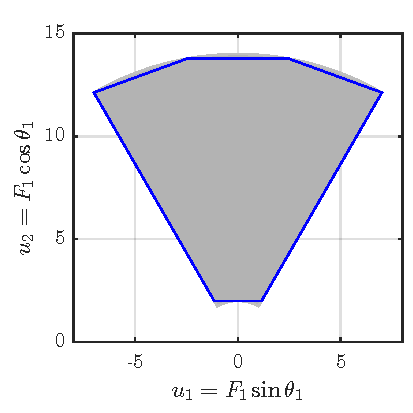
\includegraphics[]{Bicopter/BicopterInputConstraintApprox.pdf}
 \caption{Approximation of the Bicopter input constraints}
 \label{fig:BicopterInputConstraintApprox}
\end{figure}

\paragraph{Reference trajectory.}
A possible left complement for $\sysInputMat$ is
\begin{align}
 (\sysInputMatLComp)^\top = \begin{bmatrix} \PropPosZ & 0 & 0 & 0 & -1 & 0 \\ 0 & \PropPosY' & 0 & -\sin\PropInc & 0 & 0 \end{bmatrix}
\end{align}
With this, the matching condition for the reference from \eqref{eq:MatchingForceZeroError} is
\begin{align}
 \tuple{\lambda}^{\text{ZeroError}} = 
% \begin{bmatrix} 
%  m \PropPosZ (\vxd + \vy\wz \!-\! \vz\wy + \Rzx\gravityAccConst ) - (\Jy\wyd + (\Jx-\Jz)\wx\wz)  \\
%  \PropPosY' m (\vyd + \vx\wz \!-\! \vz\wx + \Rzy\gravityAccConst) - \sin\PropInc (\Jx \wxd + (\Jz-\Jy)\wy\wz)
% \end{bmatrix}
 \begin{bmatrix} 
  m \PropPosZ  \big( \vxd + \vy\wz \!-\! \vz\wy - \epsx (\wyd + \tfrac{\Jx-\Jz}{\Jy} \wx\wz) + \Rzx\gravityAccConst \big)  \\
  m \PropPosY' \big( \vyd + \vx\wz \!-\! \vz\wx + \epsy (\wxd + \tfrac{\Jz-\Jy}{\Jx} \wy\wz) + \Rzy\gravityAccConst \big)
 \end{bmatrix}
 = \tuple{0}
 .
\end{align}
where
\begin{align}
 \epsx = -\tfrac{\Jy}{\m \PropPosZ},
\qquad
 \epsy = \tfrac{\Jx \sin\PropInc}{\m (\PropPosY \cos\PropInc - \PropPosZ \sin\PropInc)}.
\end{align}
For the general case\footnote{Even in the case $\epsx=\epsy\neq0$ we would need $\Jx=\Jy=\Jz$ for $\r+\R \tuple{\eps}$ to be a flat output. The case $\epsx=0$ implies $\Jy=0$, which does not make physical sense.} 
$\epsx\neq\epsy$ this system is probably not flat, so parameterization of a feasible reference trajectory is not trivial.

\paragraph{Closed loop template.}
As for the quadcopter, the closed loop templates are that of a free rigid body i.e.\ \autoref{sec:CtrlApproachParticlesSingleBody}, \autoref{sec:CtrlApproachBodySingleBody} and \autoref{sec:CtrlApproachEnergySingleBody}.
However, in contrast to the quadcopter there are no assumtions on symmetries in the constitutive parameters.

\paragraph{Matching.}
As before we first consider the linearized matching condtions:
It turns out that asymmetries in the constitutive parameters are not useful for resolving matching constraints.
So we set $\Jcxy=\Jcxz=\Jcyz=0$, $\scx=\scy=0$ and the same for damping and stiffness.
The remaining linearized matching conditions may be fulfilled by constraining the parameters as
\begin{subequations}
\begin{align} 
 \lcz = \hcz,
\qquad
 \sigcx = \sigcy = 0,
\qquad
 \kapcx = \kapcy = \mc \gravityAccConst (\hcz-\scz),
\\
 \Jcx = \mc (\hcz-\scz)(\scz-\epsy),
\qquad
 \Jcy = \mc(\hcz-\scz) (\scz-\epsx),
\end{align}
\end{subequations}
which leaves the tuning parameters $\mc, \dc, \kc, \scz, \hcz$ and $\Jcz, \sigcz, \kapcz$.
Note, in contrast to the quadcopter, that $\epsx \neq \epsy$ implies $\Jcx \neq \Jcy$ and since the remaining relevant parameters are identical, the closed loop dynamics for x and y are different from another.

The remaining matching force in the stabilization case $\sysVelR = \tuple{0}$ is
\begin{align}
 \tilde{\sysForce} = \frac{\mc}{m}
 \begin{bmatrix} \frac{1}{\hcz-\epsx} & 0 \\ 0 & \frac{1}{\hcz-\epsy} \\ 0 & 0 \\ 0 & -\frac{\epsy}{\hcz-\epsy} \\ \frac{\epsx}{\hcz-\epsx} & 0 \\ 0 & 0 \end{bmatrix}
 \begin{bmatrix}
  \big( \Jcz - \mc(\hcz-\scz) (\tfrac{\Jx-\Jz}{\Jy}\epsx - \epsy) \big) \wy\wz - \tfrac{1}{2} \kapcz (\RExz+\REzx) \\
  \big( \Jcz - \mc(\hcz-\scz) (\tfrac{\Jy-\Jz}{\Jx}\epsy - \epsx) \big) \wx\wz - \tfrac{1}{2} \kapcz (\REyz+\REzy)
 \end{bmatrix}
\end{align}

\paragraph{Simulation result.}
Since the bicopter model is probably not flat, generation of a feasible reference trajectory is not trivial. 
For the simulation example here we exploited that, if we set $\rRx = 0$ and $\RRxx=1$, the motion is constrained to the yz plane and the remaining model is essentially a PVTOL.
The reference trajectory chosen for this example is a vertical circle with constant arc speed in the yz plane, similar to the examples presented in \cite{Konz:AT} and \cite{Konz:GaussTrackingControl}.
As shown in \autoref{sec:CtrlExamplePVTOL}, the position trajectory determines the tilt trajectory through flatness.
The circle arc speed was chosen such that the bicopter is upside down at the higest point of the circle.

As initial condition for the simulation we chose a position error of $0.5\,\unit{m}$ in all directions and heading error of $90^\circ$. 
This guarantees that all parts of the control are exited.

\begin{figure}[t]
 \centering
 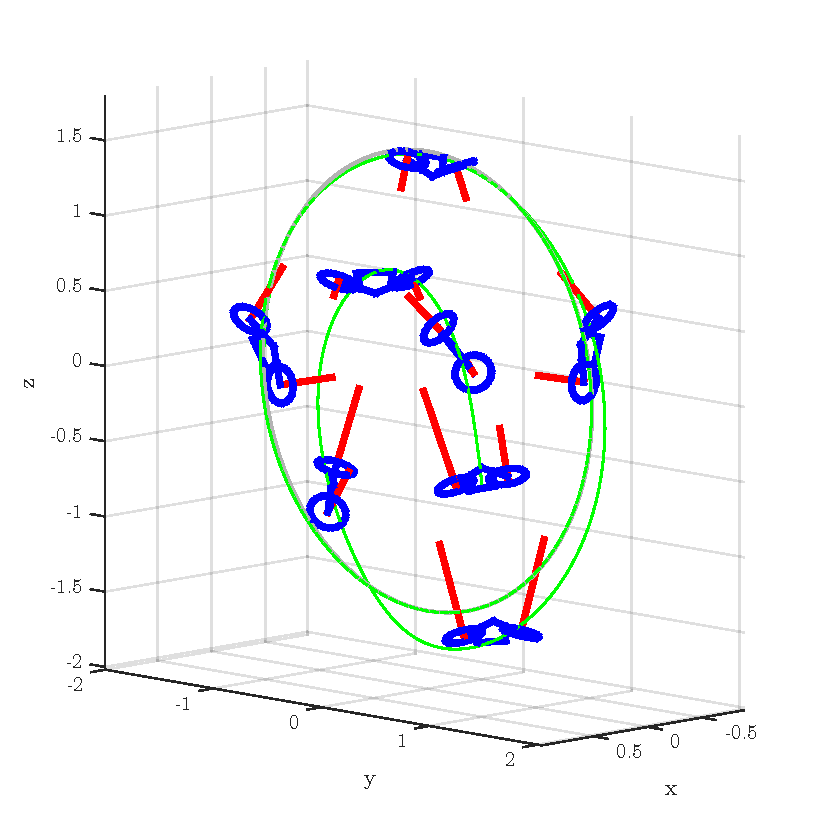
\includegraphics[]{Bicopter/BicopterCircleSimSnapshots.pdf}
 \caption{Snapshots for the simulation of the bicopter}
 \label{fig:BicopterCircleSimSnapshots}
\end{figure}

The simulation result for the position trajectory with snapshots of a bicopter mockup for the first $3\,\unit{s}$ is shown in \autoref{fig:BicopterCircleSimSnapshots}.
The red lines indicate the propeller tilt and the thurst magnitude.
The resulting time graphs are shown in \autoref{fig:BicopterCircleSimRes}.
Roughly, during the first loop, or the first $2\,\unit{s}$, the state trajectory converges to its reference and tracks it for the remaining simulation time.
This is also quantified by the error energy $\totalEnergyC$ in the bottom of \autoref{fig:BicopterCircleSimRes}.
There, one may also see that $\totalEnergyCd \neq \accCtrl{\mathcal{P}}$ which is most notably during the time around $t=0.5\,\unit{s}$ when input constraints are active, but also due to the nonvanishing matching force $\tilde{\sysForce}$.
Nevertheless, if we neglegt the parts where the input constraints are active, the error energy is converging to zero.
So, even for this arguably challenging example, the control objective is achieved.

\begin{figure}[p]
 \centering
 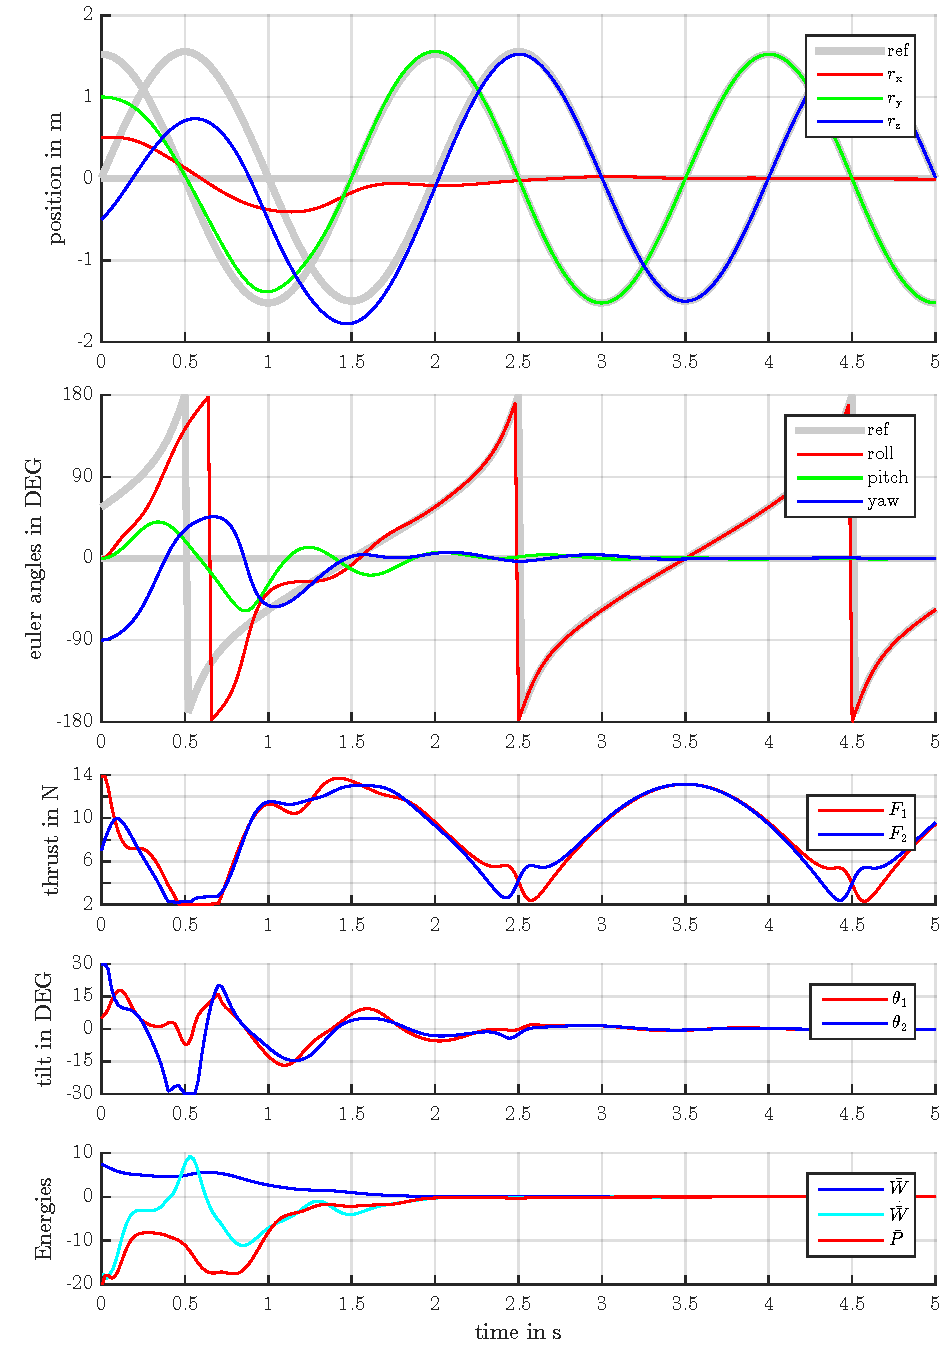
\includegraphics[]{Bicopter/BicopterCircleSimRes.pdf}
 \caption{Simulation result for the bicopter}
 \label{fig:BicopterCircleSimRes}
\end{figure}

 
\chapter{Multicopter control realization}\label{sec:MulticopterRealization}

\begin{figure}[ht]
 \centering
 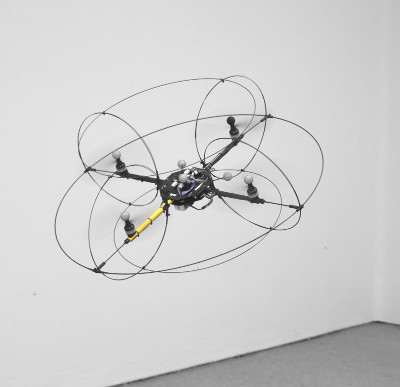
\includegraphics[height=5.5cm]{QuadV4.jpg}
 \hspace{.05\linewidth}
 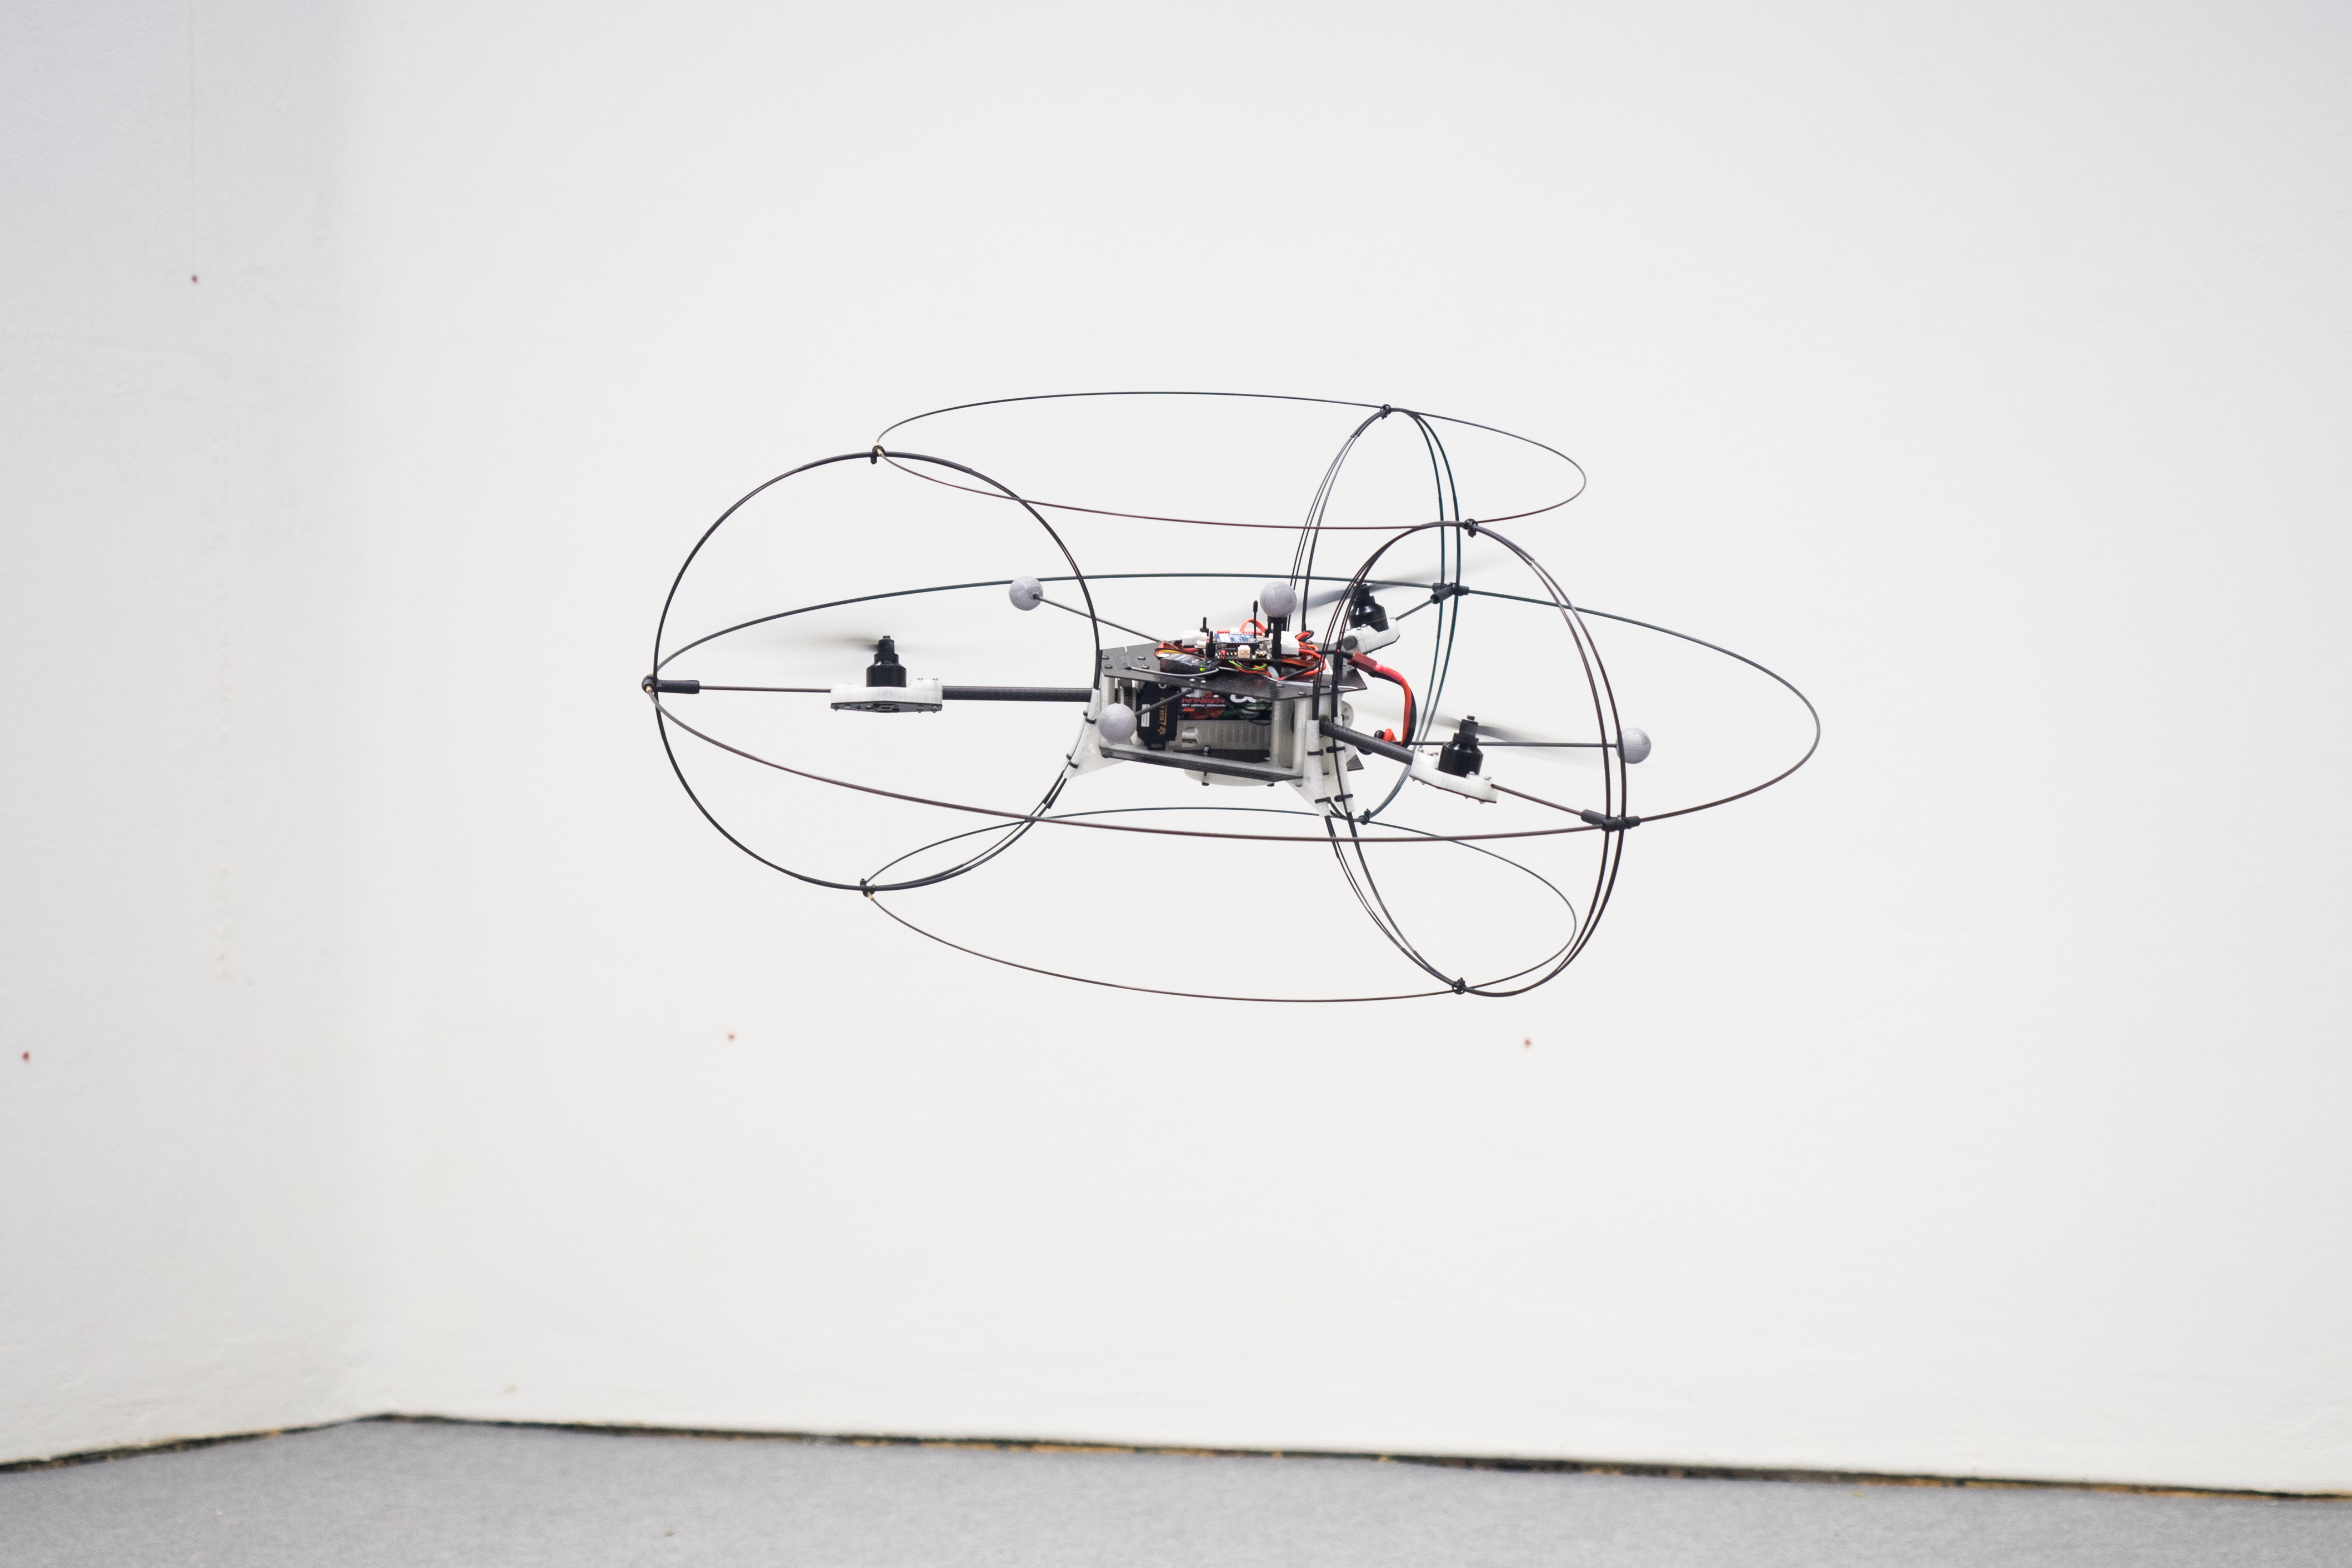
\includegraphics[height=5.5cm]{TriV4.jpg}
 \caption{LSR-Quad- and Tricopter}
 \label{fig:LSRQuadAndTri}
\end{figure}

This chapter describes the realization and discusses the experimental results with the LSR-Multicopters, \autoref{fig:LSRQuadAndTri}.
On the highest abstraction layer they can be regarded as a single rigid body with body fixed forces (the propeller forces and torques).
As such they are used for practical validation of the modeling and control approaches of the previous chapters.

The LSR-quadcopter started as a student project in 2009, a time in which they were not as ubiquitous as these drones are nowadays, 15 years later.
The original hardware, a kit from the online shop \url{www.mikrokopter.de}, was continuosly improved and addapted for specific experiments until the only remaining original parts in 2018 were the motors and propellers.
The final version has an outer diameter of $0.8\,\unit{m}$ and a weight of about $1\,\unit{kg}$.
With a maximal total propeller thrust of rougly $3.2\,\unit{kg}$ there is a lot of reserve for aggressive maneuvering. 

Based on experiences with the quadcopter, the LSR-tricopter also started as a student project in 2012.
It utilizes three tiltable propellers, which makes it from a control perspective a fully actuated free rigid body.
Its propellers and outer dimensions are the same as the quadcopter.
Due to the additional servo motors and the tilting joints the overall weigt is higher at about $1.3\,\unit{kg}$.
Furthermore, due to the $120^\circ$ arrangement of the arms, the propellers may counteract each other when tilted, reducing the efficiency.

The ubiquity quadcopter is also reflected in the control literature.
The tricopter design in contrast, is novel, with the LSR-tricopter probably being its first practical realization.  

The LSR-multicopters were the platform for experiments in publications like \cite{Kastelan:Tricopter}, \cite{Servais:Tricopter}, \cite{Servais:TricopterPendulumLoad}, \cite{Konz:Mechatronics}, \cite{Irscheid:HeavyRopesTricopter}, \cite{Konz:GaussTrackingControl} and several student projects, bachelor and master thesises.

\section{Hardware \& software realization}
blah \autoref{fig:LSRQuadAndTri}

\begin{figure}[ht]
 \centering
 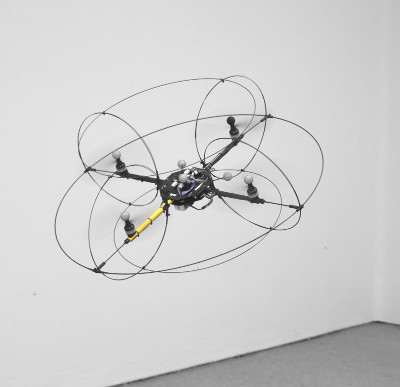
\includegraphics[width=.45\linewidth]{QuadV4.jpg}
 \hspace{.05\linewidth}
 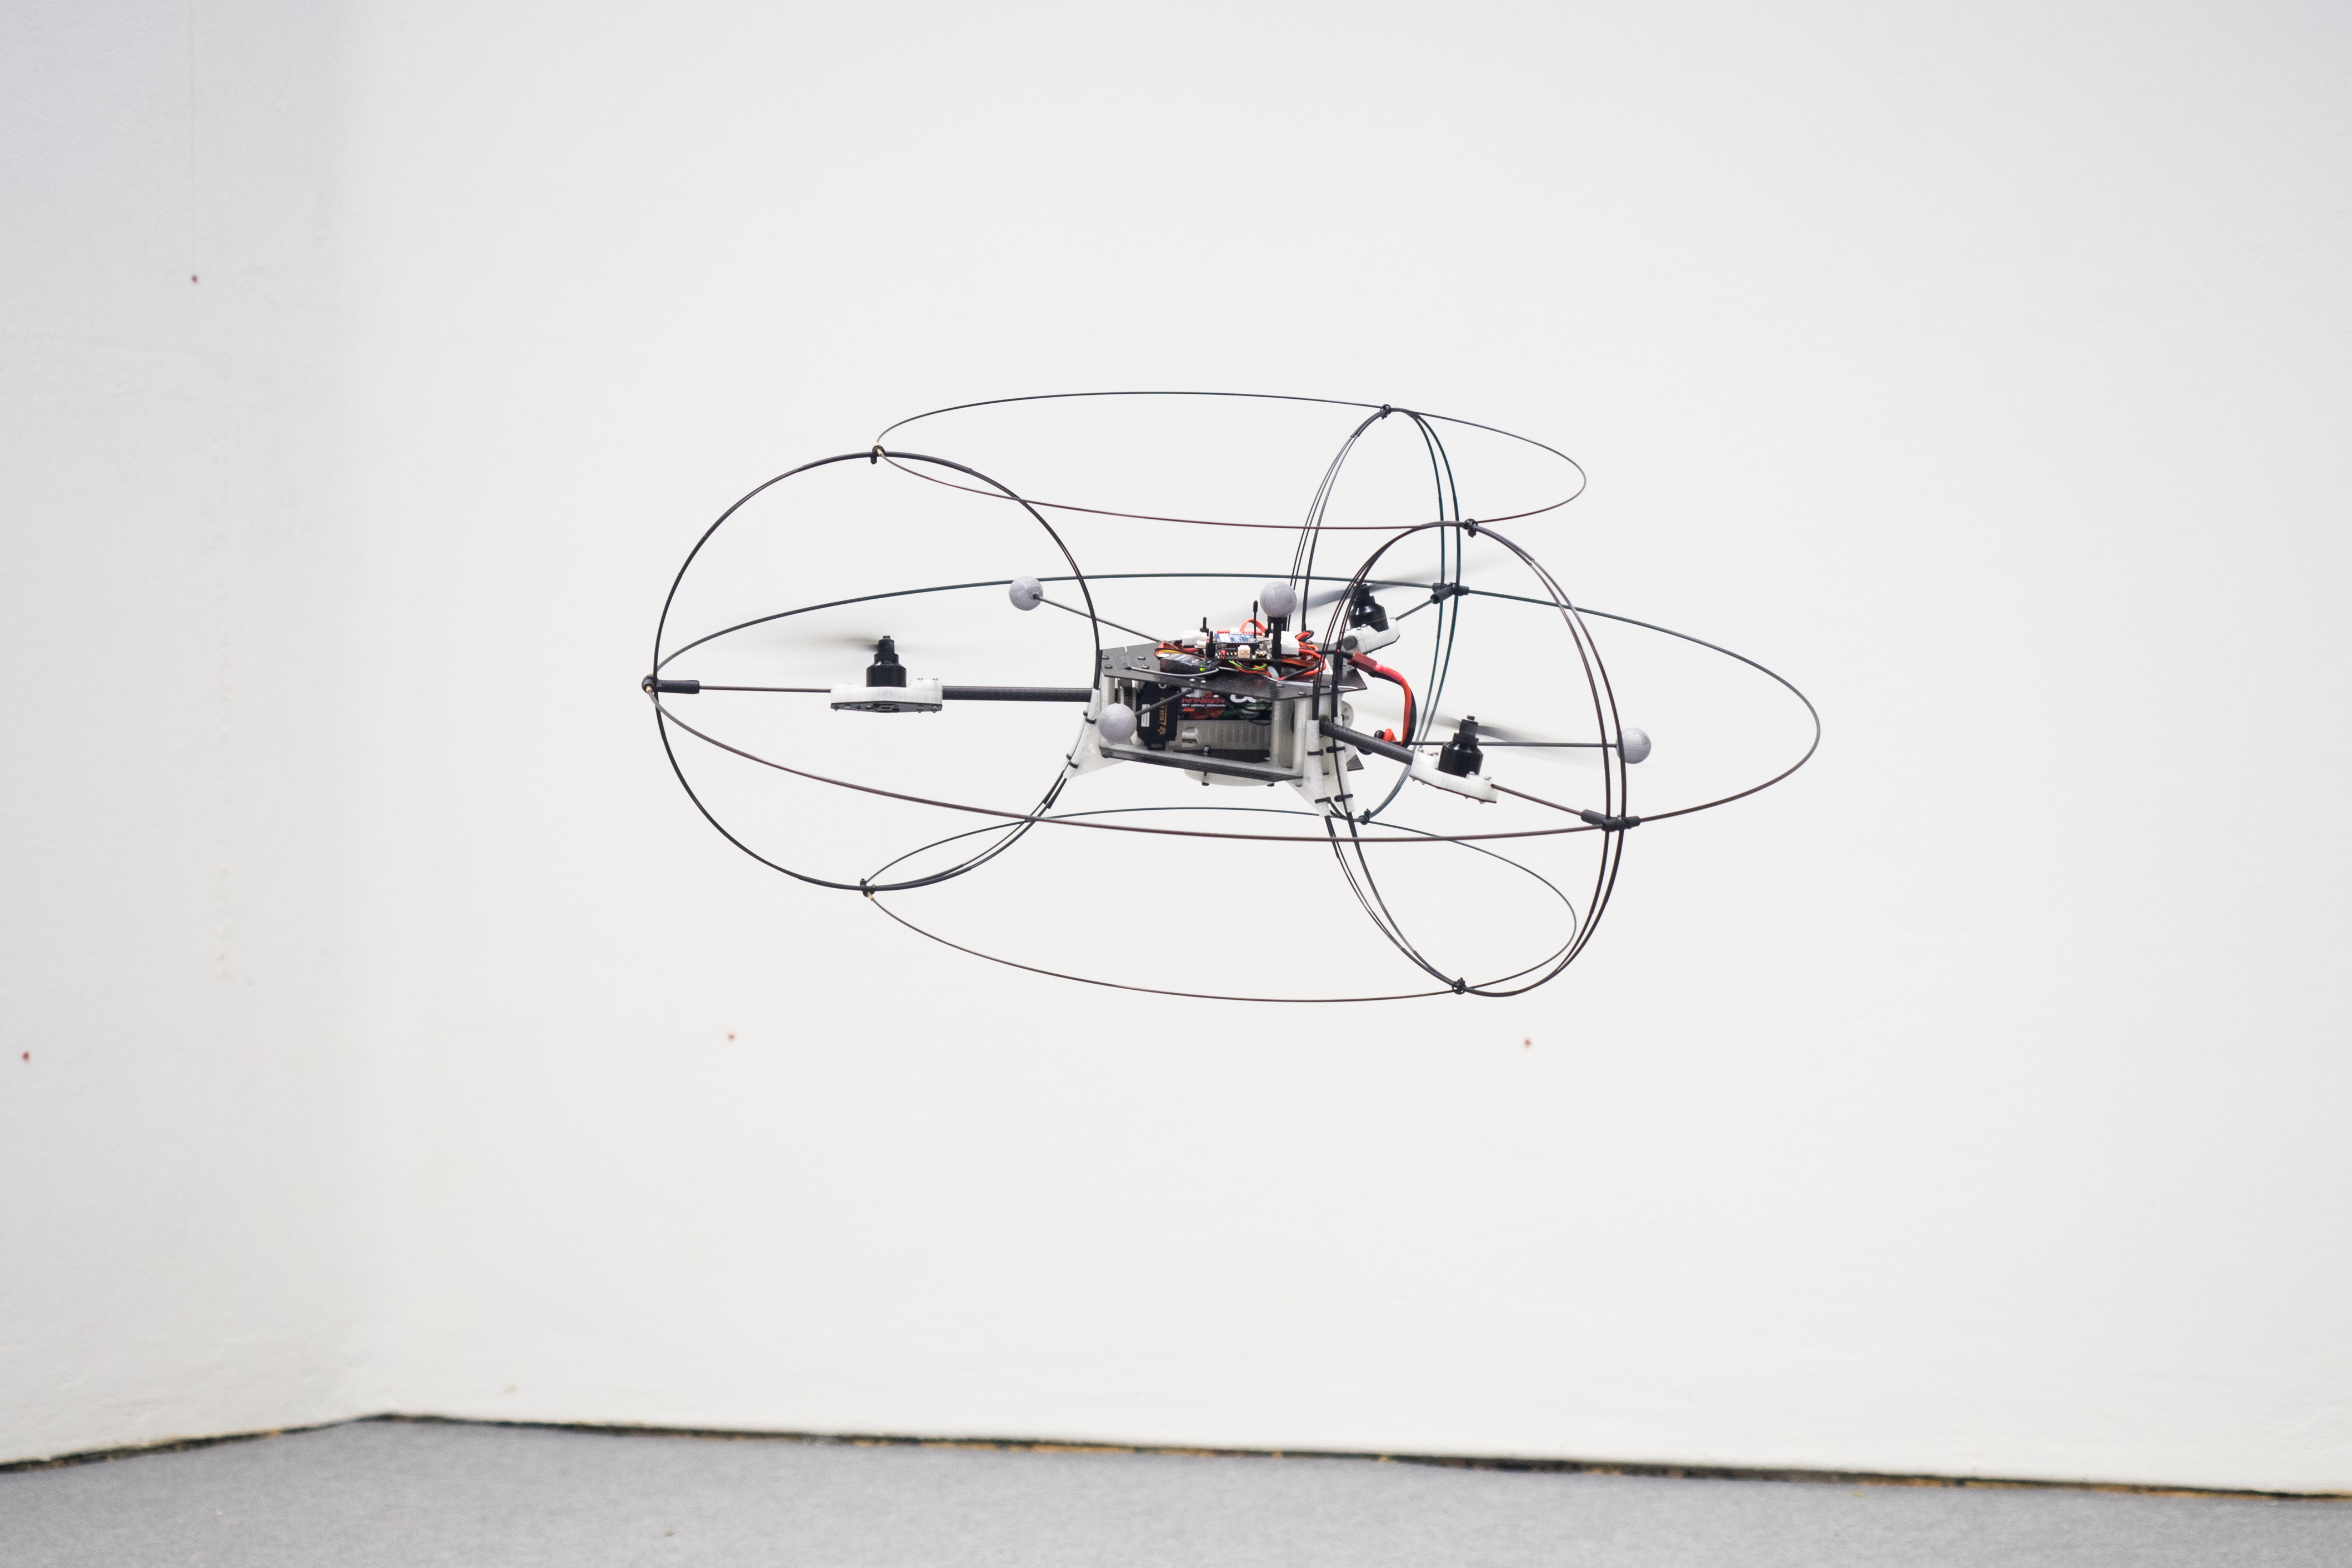
\includegraphics[width=.45\linewidth]{TriV4.jpg}
 \caption{LSR-Quad- and Tricopter}
 \label{fig:LSRQuadAndTri}
\end{figure}

The developed tricopter shown in \autoref{fig:LSRQuadAndTri} is characterized by the three independently tiltable, propeller supporting arms.
The central body and the arms are a sandwich construction of carbon-fiber plates and tubes and 3d-printed parts.
The outer carbon-fiber rings serve as collision protection and landing gear.
The vehicle has an outer diameter of about $0.8\,\unit{m}$ and a mass of about $1.2\,\unit{kg}$.

The tilting mechanism is driven by a standard hobby servo motor that is connected to a gear on the arm by a toothed-belt and allows for tilt angles of $\pm 75^\circ$.
The three $10\,\unit{inch}$ propellers are each driven by a brushless dc-motor (BLDC) capable of angular velocities up to $120\,\unit{Hz}$, corresponding to a maximum thrust of $8\,\unit{N}$.
As energy source the tricopter carries a $14.8\,\unit{V}$, $2.2\,\unit{Ah}$ LiPo battery that allows for up to $15\,\unit{min}$ of autonomous flight.

Two types of sensors are used by the tricopter:
An inertial measurement unit (IMU) VN100s from \textsc{VectorNav} is mounted on the central body to measure its angular velocity and acceleration and provide attitude estimates.
An external camera-based motion capture system from \textsc{Vicon} measures position and attitude by way of reflective markers on the tricopter.

A standard two-joystick remote control is used as a reliable and near real-time user interface to the vehicle while a pair of XBee S6B Wi-Fi modules provides a two-way communication link with a groundstation PC.
The important hardware components are summarized in \autoref{fig:MulticopterRealizationOverview}.

The onboard electronics consist mainly of a custom-built mainboard and three identical motor drivers. The mainboard contains an Atmel AT32UC3C 32-bit, 66~\unit{MHz} microcontroller with FPU and is tasked with executing all control algorithms.
Although compact brushless-dc motor drivers are ubiquitous, available products typically lack explicit speed control. 
Moreover, while the rotor speed is implicitly known to the driver through electrical commutation, speed feedback necessary for an external control implementation is usually not provided. 
As a result, a custom module was developed that provides such a measurement while implementing an underlying current controller to drive the motor. 
This solution allows for rapid propeller dynamics described further in (??) that include active braking, achieved by feeding current back into the battery.


\begin{figure}[t]
 \centering
 \footnotesize
 \newcommand{\macGroundstation}{\textcolor{white}{\textbf{Groundstation} (Win7 PC)}}
 \newcommand{\macMulticopterRealization}{\textcolor{white}{\textbf{Multicopter}}}
 \newcommand{\macRBSI}{\textcolor{white}{\textbf{rigid}}}
 \newcommand{\macRBSII}{\textcolor{white}{\textbf{body}}}
 \newcommand{\macRBSIII}{\textcolor{white}{\textbf{system}}}
 \newcommand{\macMCI}{\textcolor{white}{\textbf{main}}}
 \newcommand{\macMCII}{\textcolor{white}{\textbf{controller}}}
 \input{graphics/MulticopterRealizationOverview.pdf_tex}
 \caption{Multicopter Hardware realization}
 \label{fig:MulticopterRealizationOverview}
%\end{figure}
\vspace{5mm}
 \input{graphics/MicocontrollerCodeStructure.pdf_tex}
 \caption{Controller code structure}
 \label{fig:MicocontrollerCodeStructure}
%\begin{figure}[hb]
% \vspace{5mm}
%  \footnotesize
%  \input{graphics/StructureMulticopterAgent.pdf_tex}
%  \caption{Structure of the Multicopter Agent}
%  \label{fig:StructureMulticopterAgent}
\end{figure}
\section{Multicopter Models}\label{sec:RealizationModels}
This section derives a mathematical model for a multicopter based on the theory and the example from \autoref{sec:RBSRigidBodySys}.
Furthermore, it covers parametrer identification, model simplifications and validation with the LSR quad and tricopter.
The resulting models are the basis for simulation and controller design. 

\subsection{Actuator models}

\paragraph{Propeller motor.}
A multicopter propeller is mounted on a small brushless DC motor (BLDC) which is controlled by dedicated driver electronics.
This driver implements the electronic commutation and a digital current control with sampling frequency of $64\,\unit{kHz}$.
It recieves the desired, torque generating current $\BLDCCurr$ from the maincontroller with the sampling frequency of $200\,\unit{Hz}$. 
Consequently we assume that all electrical dynamics of the propeller drive are negligible on the timescale of the main controller and the motor torque on the propeller is proportional to its current as
\begin{align}
 \BLDCTorque = \BLDCTorqueConstant \BLDCCurr.
\end{align}

\paragraph{Servo motor.}
On the tricopter there are servo motors controlling the tilt $\aServo$ of the propellers.
These are standard hobbyist servos which combine a small motor, a gearbox, a potentiometer and some digital controller which takes the desired servo angle $\aServoR$ as input.
The integrated controller is probably a fast PID controller since it handles constant loads as well as fast transitions quite well.
However, at the maincontroller sampling frequency, $200\,\unit{Hz}$, the fast internal dynamics are neglectable and for modeling we only assume a PD controller
\begin{align}
 \ServoTorque = \ServoKP (\aServoR - \aServo) - \ServoKD \aServod.
\end{align}
Comparison of the resulting model and actual measurments in \autoref{fig:ServoSimRes}, show that this assumtion is valid here.

\paragraph{Propeller aerodynamics.}
Propellers are designed to generate a force in its spinning direction.
A general theory of propellers is quite sophisticated, see e.g.\ \cite{Johnson:HelicopterTheory}.
However, for the small, rigid propellers used on the LSR quad and tricopter a simple model, which is also common in the corresponding literature e.g.\ \cite{Mahony:Quadrotor2002}, \cite{MellingerIJRR12} or \cite{Fritsch:Diss}, is sufficient:
\begin{align}\label{eq:RealizationModelPropeller}
 \PropForce = \kappaF \PropVel^2,
\qquad
 \PropTorque = -\kappaT \PropVel^2.
\end{align}
where $\PropVel$ is the angular velocity of the propeller.
The propeller thrust $\PropForce$ is directed along its spinning direction and the propeller drag $\PropTorque$ acts opposing the spinning direction.
The model parameters $\kappaF$ and $\kappaT$ arise from the propeller geometry but will be identified in dedicated experiments.

In \cite{Bristeau:Propeller} and \cite{Martin:AccelerometerFeedback} a more sophisticated aerodynamic model for a quadcopter of about the same size as the one used here is proposed.
It mainly adds dissipative forces that are bilinear in the propeller velocities $\PropVel$ and the rigid body velocities $\v$ and $\w$.
For this it introduces 8 additional constant model parameters.
Even though their model has a nice physical motivation, it does not fit to the experimental observations done for this work.
It does, however, motivate linear drag force and torques on the multicopter body.

\paragraph{Dissipative forces.}
We assume a general linear damping model for the overall multicopter as motivated in \autoref{sec:DampingSE3}
\begin{align}
 \begin{bmatrix} \tuple{\bodyForceSym}_D \\ \tuple{\bodyTorqueSym}_D \end{bmatrix}
 &= 
 \begin{bmatrix} \mat{D}_v & \mat{D}_v \wedOp(\bodyCOD{}{})^\top \\ \wedOp(\bodyCOD{}{}) \mat{D}_v & \bodyMOD{}{} \end{bmatrix}
 \begin{bmatrix} \v \\ \w \end{bmatrix}
\end{align}
where the parameters $\mat{D}_v = \diag(\dvx, \dvx, \dvz)$, $\bodyCOD{}{}{} = [0,0,\lz]^\top$, $\bodyMOD{}{}{} = \diag(\sigx, \sigx, \sigz)$ reflect the geometric symmetries of the multicopters.


\subsection{Rigid body model}
A rigid body model for a tricopter with tiltable propellers has been discussed in \autoref{sec:RBSRigidBodySys}.
Here we like to present a generic model for a multicopter with $\numProp$ tiltable propellers.
The specific model for a quadcopter and a tricopter arises by application of special parameter values.

\paragraph{Coordinates and Kinematics.}
Recalling from \autoref{sec:RBSRigidBodySys}, we choose the configuration coordinates 
\begin{align}
 \sysCoord = \big[ \r^\top, \vectorize(\R)^\top, \tuple{\PropTilt}^\top, \tuple{\PropAngle}^\top \big]^\top \in \RealNum^{12+2\numProp}
\end{align}
where $\r \in \RealNum^3$ is the position of the center body, $\R \in \SpecialOrthogonalGroup(3)$ its orientation matrix, $\tuple{\PropTilt} = [\PropTilt[1], \ldots, \PropTilt[\numProp]]^\top \in \RealNum^{\numProp}$ the arm tilt angles and $\tuple{\PropAngle} = [\PropAngle[1],\ldots,\PropAngle[\numProp]]^\top \in \RealNum^{\numProp}$ the angles of the propellers, see \autoref{fig:TricopterInputs}.
Note that the propellers are designed only for either clockwise or counter-clockwise rotation, and will only rotate in this direction during operation.
The propeller angles $\PropAngle[k]$ are defined, such that $\PropAngled[k] > 0$ during operation.
To recover the spinning directions we use the parameter $\PropDir[k] = 1$ for a positive/counter-clockwise and $\PropDir[k] = -1$ for a negative/clockwise spinning propeller.

\begin{figure}
 \centering
 \input{graphics/TricopterInputs.pdf_tex}
 \caption{Mechanical model of the tricopter}
 \label{fig:TricopterInputs}
\end{figure}

To capture the velocity state of the system we use the velocity coordinates
\begin{align}
 \sysVel = \big[ \v, \w, \dot{\tuple{\PropTilt}}, \tuple{\PropVel}]^\top \in \RealNum^{6+2\numProp},
\end{align}
related to the configuration coordinates by
\begin{align}
 \rd = \R \v, 
\qquad
 \Rd = \R \wedOp(\w),
\qquad
 \dot{\tuple{\PropAngle}} = \tuple{\PropVel}.
\end{align}

\paragraph{Assumtions on the mass distribution.}
The algorithm proposed in \autoref{sec:RBSRigidBodySys} does of course handle general mass distributions of the rigid bodies, but the resulting kinetic equations are far too cumbersome to display here explicitly.
Instead we motivate some assumptions on the body inertia matrices that will lead to a greatly condensed system inertia matrix:
Assume that the combined center of mass of one arms and its propeller lies on the tilt axis.
This implies that the overall center of mass $\bodyCOM{}{}{} \in \RealNum^{3}$ of the complete system is constant w.r.t.\ the body fixed frame.
This was one goal during the construction process of the Tricopter.
Furthermore, we assume that the combined moment of inertia of one arm and propeller is symmetric about the tilt axis.
This is not the case for the real inertia parameters.
However, it is justified by the fact that the overall inertia $\bodyMOI{}{}{}$ changes only slightly depending on the arm tilts $\PropTilt$ or the propeller angles $\PropAngle$.  

A crucial part to get the overall dynamics right, is to explicitly consider the rotor of the servo motor.
The relevant moment of inertia $\bodyMOISym_{\textsf{Sxx}}$ might be very small, but since it is located behind a gearbox with transmission ratio $c_{\mathsf{S}} = 625$ its contribution to the system inertia matrix is significant.
This is reflected in the different values within $\JAC$ which contains $c_{\mathsf{S}} \bodyMOISym_{\textsf{Sxx}}$ and $\JA$ which contains $c_{\mathsf{S}}^2 \bodyMOISym_{\textsf{Sxx}}$.
The validity of the model with these assumptions will be discussed later by comparison to experimental data.

\paragraph{Kinetic equation.}
With the above assumptions, and the propeller model \eqref{eq:RealizationModelPropeller}, the kinetic equation for a multicopter takes the form
\begin{align}\label{eq:RealizationMulticopterKinetics}
 \sysInertiaMat(\tuple{\PropTilt}) \sysVeld + \gyroForce(\tuple{\PropTilt}, \sysVel) + \sysDissMat \sysVel + \genForceGravity(\R) &= \genForceProp(\tuple{\PropTilt}, \PropVel) + \genForceInput(\BLDCTorque, \ServoTorque) + \genForceBias
\end{align}
where
\begin{subequations}\label{eq:RealizationMulticopterForces}
\begin{align}
 \sysInertiaMat(\tuple{\PropTilt}) &=
 \begin{bmatrix}[1.1]
  \m \idMat[3] & \m \wedOp(\bodyCOM{}{})^\top & 0 & 0 \\
  \m \wedOp(\bodyCOM{}{}) & \bodyMOI{}{}{} & \JAC \mat{H}_1 & \JP \mat{H}_3(\tuple{\PropTilt}) \diag(\tuple{\PropDir}) \\
  0 & \JAC \mat{H}_1^\top & \ArmInertia \idMat[\numProp] & 0 \\
  0 & \JP \diag(\tuple{\PropDir}) \mat{H}_3^\top(\tuple{\PropTilt}) & 0 & \PropInertia \idMat[\numProp]
 \end{bmatrix},
\\
 \gyroForce(\tuple{\PropTilt}, \sysVel) &= 
 \begin{bmatrix}[1.1]
  \wedOp(\w) \tuple{\genMomentumSym}_{\v} \\
  \wedOp(\v) \tuple{\genMomentumSym}_{\v} + \wedOp(\w) \tuple{\genMomentumSym}_{\w} + \JP \mat{H}_4(\tuple{\PropTilt}) \diag(\dot{\tuple{\PropTilt}}) \diag(\tuple{\PropDir}) \tuple{\PropVel} \\
  -\JP \diag( \diag(\tuple{\PropDir}) \mat{H}_4^\top(\tuple{\PropTilt}) \w) \tuple{\PropVel} \\
   \JP \diag( \diag(\tuple{\PropDir}) \mat{H}_4^\top(\tuple{\PropTilt}) \w) \dot{\tuple{\PropTilt}} \\
 \end{bmatrix},
\\
 \sysDissMat &= \begin{bmatrix} \mat{D}_v & \mat{D}_v \!\wedOp(\bodyCOD{}{})^\top\! & 0 & 0 \\ \wedOp(\bodyCOD{}{}) \mat{D}_v & \bodyMOD{}{}{} & 0 & 0 \\ 0 & 0 & 0 & 0 \\ 0 & 0 & 0 & 0 \end{bmatrix}\!,
\quad
 \genForceGravity(\R) = \begin{bmatrix}[1.1] \m \idMat[3] \\ \m \wedOp(\bodyCOM{}{}) \\ 0 \\ 0 \end{bmatrix} \RT (-\gravityAcc),
\\
 \genForceProp(\tuple{\PropTilt}, \tuple{\PropVel}) &= \begin{bmatrix} \kappaF \mat{H}_3(\tuple{\PropTilt}) \\ \kappaF \big( \ArmRadius \mat{H}_4(\tuple{\PropTilt}) + \ArmHeight \mat{H}_2(\tuple{\PropTilt}) \big) - \kappaT \mat{H}_3(\tuple{\PropTilt}) \diag(\tuple{\PropDir}) \\ 0 \\ -\kappaT \idMat[\numProp] \end{bmatrix} \diag(\tuple{\PropVel}) \tuple{\PropVel},
\\
 \genForceInput(\BLDCTorque, \ServoTorque) &= \begin{bmatrix} 0 \\ 0 \\ \ServoTorque \\ \BLDCTorque \end{bmatrix}
\qquad
 \genForceBias = \begin{bmatrix} \FB \\ \tauB \\ 0 \\ \BLDCFriction \end{bmatrix}
\end{align}
with the (just for readability) substituted momenta
\begin{align}
 \tuple{\genMomentumSym}_{\v} &= m (\v - \wedOp(\bodyCOM{}{}) \w), 
\\
 \tuple{\genMomentumSym}_{\w} &= m \wedOp(\bodyCOM{}{}) \v + \bodyMOI{}{}{} \w + \JAC \mat{H}_1 \dot{\tuple{\PropTilt}}  + \JP \mat{H}_3(\tuple{\PropTilt}) \diag(\tuple{\PropDir}) \tuple{\PropVel}.
\end{align}
and the sub-matrices
\begin{align}
 \mat{H}_1 &= \begin{bmatrix}
  \cArmAngle[1] & \cdots & \cArmAngle[\numProp] \\
  \sArmAngle[1] & \cdots & \sArmAngle[\numProp] \\
  0 & \cdots & 0
 \end{bmatrix}\!,&
 \mat{H}_2(\tuple{\PropTilt}) &= \begin{bmatrix}
  \cArmAngle[1] \sPropTilt[1] & \cdots & \cArmAngle[\numProp] \sPropTilt[\numProp] \\
  \sArmAngle[1] \sPropTilt[1] & \cdots & \sArmAngle[\numProp] \sPropTilt[\numProp] \\
  0 & \cdots & 0
 \end{bmatrix}\!,
\\
 \mat{H}_3(\tuple{\PropTilt}) &= \begin{bmatrix}
   \sArmAngle[1] \sPropTilt[1] & \cdots &  \sArmAngle[\numProp] \sPropTilt[\numProp] \\
  -\cArmAngle[1] \sPropTilt[1] & \cdots & -\cArmAngle[\numProp] \sPropTilt[\numProp] \\
   \cPropTilt[1]               & \cdots &  \cPropTilt[\numProp]                     
 \end{bmatrix}\!,&
 \mat{H}_4(\tuple{\PropTilt}) &= \begin{bmatrix}
  \sArmAngle[1] \cPropTilt[1] & \cdots & \sArmAngle[\numProp] \cPropTilt[\numProp] \\
  -\cArmAngle[1] \cPropTilt[1] & & -\cArmAngle[\numProp] \cPropTilt[\numProp] \\
  -\sPropTilt[1] & \cdots & -\sPropTilt[\numProp]
 \end{bmatrix}
% \quad \tdiff{t} \big( \mat{H}_3(\tuple{\PropTilt}) \big) = \mat{H}_3'(\tuple{\PropTilt}) \diag(\dot{\tuple{\PropTilt}})
.
\end{align}
\end{subequations}

\paragraph{Tricopter.}
To get the rigid body model equations for the tricopter (displayed in \autoref{fig:TricopterInputs}) we plug the following parameters into \eqref{eq:RealizationMulticopterForces}
\begin{align}
 \numProp = 3,
\qquad
%  \ArmAngle[1] = \tfrac{\pi}{3}, \
%  \ArmAngle[2] = \pi, \
%  \ArmAngle[3] = -\tfrac{\pi}{3},
 \ArmAngle = \tfrac{\pi}{3} [1, 3, 5]^\top,
\qquad
%  \PropDir[1] = -1, \
%  \PropDir[2] = \PropDir[3] = 1.
 \PropDir = [-1, +1, +1]^\top.
\end{align}
The model equations do not simplify too much and the special result is not displayed explicitly here.

\paragraph{Quadcopter.}
For the quadcopter model we have the parameters (see \autoref{fig:QuadcopterInputs})
\begin{align}
 \numProp = 4,
\qquad
%  \ArmAngle[1] = 0, \
%  \ArmAngle[2] = \tfrac{\pi}{2}, \
%  \ArmAngle[3] = \pi, \
%  \ArmAngle[4] = -\tfrac{\pi}{2},
 \ArmAngle = \tfrac{\pi}{2} [0, 1, 2, 3]^\top,
\qquad
%  \PropDir[1] = \PropDir[3] = 1, \
%  \PropDir[2] = \PropDir[4] = -1,
 \tuple{\PropDir} = [+1, -1, +1, -1]^\top,
\qquad
% \PropTilt[1] = \PropTilt[2] = \PropTilt[3] = \PropTilt[4] = 0.
 \PropTilt = [0, 0, 0, 0]^\top.
\end{align}
Here the model equations simplify significantly:
Since the propellers do not tilt $\PropTilt = 0$, the corresponding equations can be regarded as definition of reaction torques $\ServoTorque$ and dropped from the model equations.
Overall the model for the quadcopter is
\begin{subequations}
\begin{align}
 \sysInertiaMat &=
 \begin{bmatrix}
  \m \idMat[3] & -\m \wedOp(\bodyCOM{}{}) & 0 \\
  \m \wedOp(\bodyCOM{}{}) & \bodyMOI{}{}{} & \JP \mat{H}_3 \diag(\tuple{\PropDir})\\
  0 & \PropInertia \diag(\tuple{\PropDir}) \mat{H}_3^\top & \PropInertia \idMat[4] \\
 \end{bmatrix},
\\
 \gyroForce(\sysVel) &= 
 \begin{bmatrix} \wedOp(\w) & 0 & 0 \\ \wedOp(\v) & \wedOp(\w) & 0 \\ 0 & 0 & 0 \end{bmatrix}
 \sysInertiaMat \sysVel,
\qquad
 \genForceGravity(\R) = \begin{bmatrix} \m \idMat[3] \\ \m \wedOp(\bodyCOM{}{}) \\ 0 \end{bmatrix} \RT (-\gravityAcc),
\\
 \genForceProp(\tuple{\PropVel}) &= \begin{bmatrix} \kappaF \mat{H}_3 \\ \kappaF \ArmRadius \mat{H}_4 - \kappaT \mat{H}_3 \diag(\tuple{\PropDir})  \\ -\kappaT \idMat[4]  \end{bmatrix} \diag(\tuple{\PropVel}) \tuple{\PropVel},
\qquad
 \genForceInput(\BLDCTorque) = \begin{bmatrix} 0 \\ 0 \\ \BLDCTorque \end{bmatrix}
\end{align}
with the sub-matrices
\begin{align}
 \mat{H}_3 &= \begin{bmatrix}
  0 & 0 & 0 & 0 \\
  0 & 0 & 0 & 0 \\
  1 & 1 & 1 & 1
 \end{bmatrix}\!,&
 \mat{H}_4 &= \begin{bmatrix}
  0 & 1 & 0 & -1 \\
  -1 & 0 & 1 & 0 \\
  0 & 0 & 0 & 0
 \end{bmatrix}\!.
\end{align}
\end{subequations}
Note that the system inertia matrix $\sysInertiaMat$ is constant, but there is still an inertial coupling between the propeller velocities $\tuple{\PropVel}$ and $\wz$.
The same model up to different dissipative forces, requiring $\bodyCOM{}{}{}=\tuple{0}$ and using Euler angles, has been derived in \cite{Martin:AccelerometerFeedback}.
%Also \cite{Mahony:Quadrotor2002} proposes a similar model, requiring $\bodyCOM{}{}{}=\tuple{0}$ and dropping some of the gyroscopic terms within $\gyroForce$.

\begin{figure}[ht]
 \centering
 \input{graphics/QuadcopterInputs.pdf_tex}
 \caption{Propeller forces on the Quadcopter}
 \label{fig:QuadcopterInputs}
\end{figure}


\subsection{Parameter identification}
The preceding mathematical model for the multicopters contains various constant parameters of which only the total mass $\m$ and the arm radius $\ArmRadius$ can be measured directly.
Some crucial parameters are identified in dedicated experimental setups which will be discussed in the following.
The remaining parameters are estimated by the method of least squares based on the system model and actual in-flight measurments.

%As mentioned before the overall rigid body system has a constant total mass $\m \in \RealNum$, combined center of mass $\bodyCOM{}{}{} \in \RealNum^3$ and combined moment of inertia $\bodyMOI{}{}{}=\bodyMOI{}{}{}^\top \in\RealNum^{3\times3}$.

\paragraph{Propeller and servo drive.}
For the identification of the propeller drive and its tilting mechanism we use a dedicated test bench, see \autoref{fig:PropellerTestBench}.
It is essentially one tricopter arm with additional absolute encoder for the tilt angle $\PropTilt$ and an incremental encoder for the propeller velocity $\PropVel$.

\begin{figure}
 \centering
 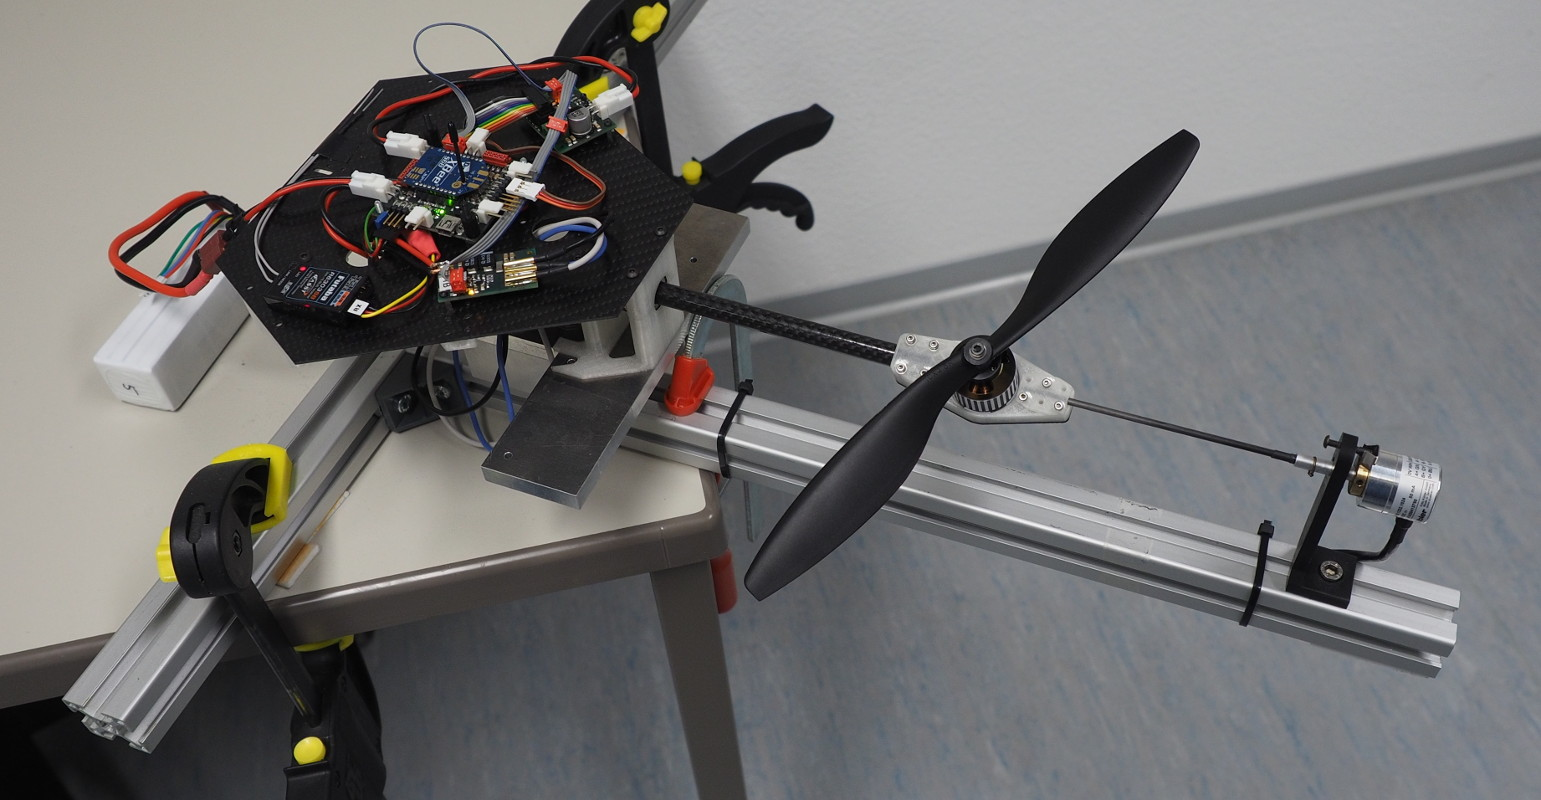
\includegraphics[width=.6\linewidth]{PropellerTestBench.jpg}
 \caption{Test bench for the propeller and tilting mechanism}
 \label{fig:PropellerTestBench}
\end{figure}
 
The equations of motion for the test bench are
\begin{align}
 \PropVeld + \underbrace{\tfrac{\kappaT}{\JP}}_{\PropParam[1]} \PropVel^2 &= \underbrace{\tfrac{\BLDCTorqueConstant}{\JP}}_{\PropParam[2]} \BLDCCurr + \underbrace{\tfrac{\BLDCFriction}{\JP}}_{\PropParam[3]}
\\
 \aServodd + \underbrace{\tfrac{\ServoKD}{\JA}}_{\ServoParam[1]} \aServod + \underbrace{\tfrac{\ServoKP}{\JA}}_{\ServoParam[0]} \aServo &= \underbrace{\tfrac{\ServoKP}{\JA}}_{\ServoParam[0]} \aServoU
\end{align}
The equations are normalized, yielding the parameters $\PropParam[1]$, $\PropParam[2]$, $\PropParam[3]$ and $\ServoParam[0]$, $\ServoParam[1]$, which will become more convenient later.
These parameters can be directly estimated from measured timeseries using Savitzky-Golay derivative estimation and the method of least squares.
The inertia parameters $\JP$ and $\JA$ are computed from a detailed CAD model of the multicopters.
With them one could recover the original parameters $\kappaT$, $\ServoKP$, etc.. 
The identified parameter values are summarized in \autoref{tab:ParamTriQuad}.

The accuracy of the proposed model and its identified parameters can be seen from the results in \autoref{fig:ServoSimRes} and \autoref{fig:PropCtrlRes} in \autoref{sec:RealizationForceVectorControl}.
An online estimation of the bias parameter $\PropParam[3]$ by means of an observer will be discussed there as well.

\paragraph*{Propeller thrust.}
For identification of the thrust constant $\kappaF$, a propeller drive was mounted horizontally on a $1\,\unit{m}$ tall pole.
The pole in turn stands on a digital scale and the ``weight'' was recorded at different propeller speeds $\PropVel$.
From this ``weight'' we can compute the corresponding propeller thrust $\PropForce$.
The measurements are displayed in \autoref{fig:PropVel2Thrust} together with the model $\PropForce = \kappaF \PropVel^2$ with the identified parameter value $\kappaF = 1.44 \cdot 10^{-5}\,\unit{N}\,\unit{s}^2$.

\begin{figure}
 \centering
 \footnotesize%
 \appendtographicspath{{graphics/PropVel2Thrust/}}%
 \begingroup%
\setlength{\unitlength}{1cm}%
\begin{picture}(12.000000,7.000000)%
\put(0,0){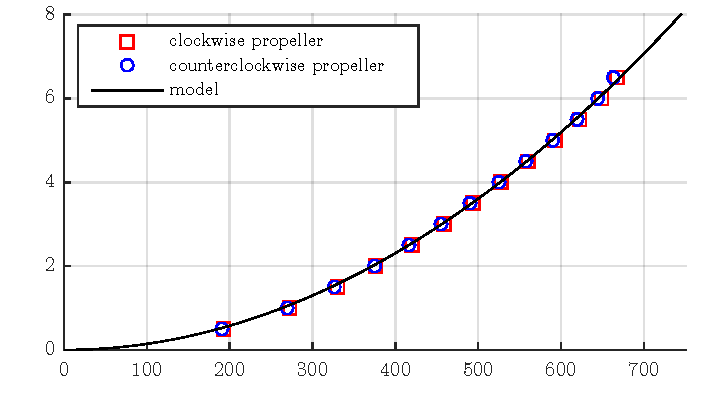
\includegraphics{PropVel2Thrust.pdf}}%
\put(6.327132, 0.157528){\makebox(0,0)[b]{\smash{$\PropVel$ in $\sfrac{\unit{RAD}}{\unit{s}}$}}}%
\put(0.522160, 3.911988){\rotatebox{90}{\makebox(0,0)[t]{\smash{$\PropForce$ in $\unit{N}$}}}}%
\end{picture}%
\endgroup%%
 \caption{Measured propeller thrust compared to proposed model}
 \label{fig:PropVel2Thrust}
\end{figure}

\paragraph*{Rigid body inertia.}
A dedicated experiment was conducted for identification of the inertia parameters $\Jxx$, $\Jyy$ and $\Jzz$ for quad and tricopter.
The body is suspended by two strings as shown on the left side of \autoref{fig:QuadPendulumIdent}.
The basic idea is that a rotation of the body about the vertical axis results in a upward movement of the body which is countered by gravity.
So we basically have a torsional spring, which, together with the inertia forms an oscillator whose frequency is proportional to the moment of inertia.

\begin{figure}
 \centering
 \input{graphics/QuadPendulumIdent.pdf_tex}
 \hfill
 \footnotesize%
 \appendtographicspath{{graphics/PendulumIdentRes/}}%
 \begingroup%
\setlength{\unitlength}{1cm}%
\begin{picture}(9.000000,6.300000)%
\put(0,0){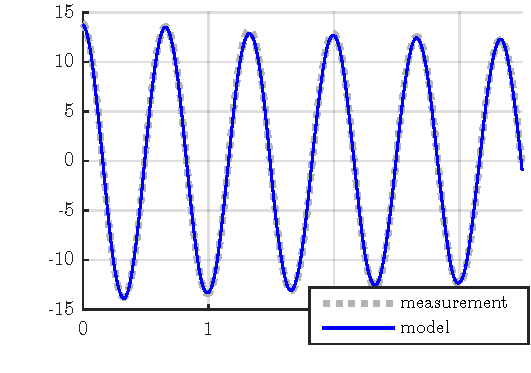
\includegraphics{PendulumIdentRes.pdf}}%
\put(5.099467, 0.138788){\makebox(0,0)[b]{\smash{$t$ in $\unit{s}$}}}%
\put(0.535099, 3.562518){\rotatebox{90}{\makebox(0,0)[t]{\smash{$\ddot{\alpha}$ in $\sfrac{\unit{RAD}}{\unit{s}^2}$}}}}%
\end{picture}%
\endgroup%%
 \caption{Experimental setup and identification result for $\Jxx$ of the Quadcopter}
 \label{fig:QuadPendulumIdent}
\end{figure}

The equation of motion for the vertical rotation with angle $\alpha$ in this setup is
\begin{align}\label{eq:PendulumIdent}
 \bodyMOISym \ddot{\alpha} + \bodyMODSym \dot{\alpha} + \m \gravityAccConst \frac{d^2 \sin\alpha}{4\sqrt{h^2 - \tfrac{d^2}{2}(1-\cos\alpha)}} = 0.
\end{align}
Here $\m$ indicated the total mass of the copter, $\gravityAccConst = 9.81\,\sfrac{\unit{m}}{\unit{s}^2}$ is the gravitational acceleration, $d$ and $h$ are the distance and length of the strings.
From the measured trajectory $t\mapsto\alpha$ of the twist angle we can estimate the inertia $\bodyMOISym$ and damping $\bodyMODSym$ about the corresponding axis.

On the right side of \autoref{fig:QuadPendulumIdent}, the acceleration $\ddot{\alpha}$ computed from the model \eqref{eq:PendulumIdent} with the estimated parameters is plotted against the measured acceleration, computed from the onboard gyroscope readings.

This test was conducted for all three axis, \ie for $\Jxx$, $\Jyy$ and $\Jzz$ for Tri- and Quadcopter and the resulting parameters are given in \autoref{tab:ParamTriQuad}.
The identified parameters match the values computed from a detailed CAD model by $\pm 10\%$.

\paragraph*{Parameter identification from flight test.}
The model \eqref{eq:RealizationMulticopterKinetics} still contains several so far unknown parameters:
The coordinates of the center of mass $\bodyCOM{}{}{} = [\sx, \sy, \sz]^\top$, the off-diagonal entries $\Jxy$, $\Jxz$ and $\Jyz$, the translational damping $\dvx$, $\dvz$, the rotational damping $\sigx$, $\sigz$ and the coordinate $\lz$ of the center of damping.

With some auxiliary transformation ($\lzp = \dvx\lz$, $\sigxp = \sigx + \dvz\lz^2$) the first 6 model equations \eqref{eq:RealizationMulticopterKinetics} are linear in the remaining unknown parameters.
So we can identify these by the method of least squares from flight test measurements.
\autoref{tab:ParamTriQuad} summarizes the identified parameter values from this flight test as well as the ones from the previously discussed dedicated experiments.
These are the values that are used for the simulator.

From this experiment we have the first estimate for the overall center of mass $\bodyCOM{}{}{}$ of tri- and quadcopter.
The identified value $\sz$ is then used to adjust the body fixed frame in the vertical direction such that $\sz=0\,\unit{m}$.
For the Tricopter this determines also the parameter $\ArmHeight$.
The values for $\sx$ and $\sy$ are small so we stick to the geometric center in the horizontal directions.

The damping parameter values for the tricopter are greater than the ones for the quadcopter.
This could be explained by the model from \cite{Martin:AccelerometerFeedback} and the fact that the propellers of the Tricopter nominally spin $40\%$ faster than on the Quadcopter.
Also the identified value for $\lz$ is roughly the distance from the body fixed frame to the propeller plane which fits well to their model.
On the other hand, the identified translational damping $\dvz$ in the vertical direction is greater than the horizontal damping $\dvx$.
This contradicts the model proposed in \cite{Martin:AccelerometerFeedback} which would imply $\dvz = 0$.

\autoref{tab:ParamTriQuad} also shows identified constant bias forces $\FB$ and torques $\tauB$ for this particular experiment.
These mean values probably result from small misalignments of the propellers and servos rather than constant side wind or anything similar.
In the practical application the bias forces will be estimated online by means of an observer, so can vary slowly.
However, the magnitudes of the displayed identified values are less than $3\%$ compared to the maximal available propeller forces $\genForceProp$ in the corresponding directions, so their influence on the overall identification result should be small.



% The scalar inertia parameters
% \begin{align}
%  \JA &= \bodyMOISym_{\mathsf{Axx}} + c_{\mathsf{S}}^2 \bodyMOISym_{\mathsf{Sxx}},&
%  \JAC &= \bodyMOISym_{\mathsf{Axx}} + c_{\mathsf{S}} \bodyMOISym_{\mathsf{Sxx}},&
% % \JP &= \bodyMOISym_{\mathsf{Pzz}},&
% \end{align}
% are related to the tilting mechanism.
% Here $\bodyMOISym_{\mathsf{Axx}}$ is the moment of inertia of the arm about the tilt axis and $\bodyMOISym_{\mathsf{Sxx}}$ the inertia of the servo motor rotor.
% What is important here is that $\JA$ and $\JAC$ take different values which would not be the case if one would not model the servo motor properly.
% For the Tricopter the estimated values are $\JA = 0.89\,\unit{kg}\,\unit{m}^2$ and $\JAC = 0.0015\,\unit{kg}\,\unit{m}^2$ which should emphasize the importance.
% 
% The remaining parameters in \eqref{eq:RealizationMulticopterKinetics} are the distances $\ArmRadius$ and $\ArmHeight$, see \autoref{fig:TricopterInputs}, the aerodynamics propeller parameters $\kappaF$ and $\kappaT$, the propeller spinning directions $\PropDir[k] = \pm 1$ and the gravity coefficients $\gravityAcc \in \RealNum^3$.
% The inertial frame was chosen to be aligned with the gravity direction, \ie $\gravityAcc = [0,0,-9.81]^\top \sfrac{\unit{m}}{\unit{s}^2}$.


\begin{table}
 \centering
 \setlength{\tabcolsep}{.1em}
 \begin{tabular}{crlrll}
  \toprule
  Symbol & \multicolumn{2}{c}{tricopter value} & \multicolumn{2}{c}{tuadcopter value} & \multicolumn{1}{c}{Source} \\
  \midrule
  $\quad\m\quad$ & $1.251$&$\unit{kg}$ & $1.001$&$\unit{kg}$ & directly measured
  \\[1ex]
  $\sx$ & $ 1.7 \cdot 10^{-3}$&$\unit{m}$ & $ -1.8 \cdot 10^{-3}$&$\unit{m}$ & flight test \\
  $\sy$ & $ 0.6 \cdot 10^{-3}$&$\unit{m}$ & $ 0.6 \cdot 10^{-3}$&$\unit{m}$ & flight test \\
  $\sz$ & $ 0.0 \cdot 10^{-3}$&$\unit{m}$ & $ 0.0 \cdot 10^{-3}$&$\unit{m}$ & manually adjusted
  \\[1ex]
  $\Jxx$ & \phantom{|} \qquad $19.2 \cdot 10^{-3}$&$\unit{kg}\,\unit{m}^2$ \qquad \phantom{|} & \phantom{|} \qquad $17.9 \cdot 10^{-3}$&$\unit{kg}\,\unit{m}^2$ \qquad \phantom{|} & pendulum test\\
  $\Jyy$ & $19.2 \cdot 10^{-3}$&$\unit{kg}\,\unit{m}^2$ & $18.0 \cdot 10^{-3}$&$\unit{kg}\,\unit{m}^2$ & pendulum test \\
  $\Jzz$ & $30.8 \cdot 10^{-3}$&$\unit{kg}\,\unit{m}^2$ & $30.7 \cdot 10^{-3}$&$\unit{kg}\,\unit{m}^2$ & pendulum test \\
  $\Jxy$ & $-0.8 \cdot 10^{-3}$&$\unit{kg}\,\unit{m}^2$ & $-0.7 \cdot 10^{-3}$&$\unit{kg}\,\unit{m}^2$ & flight test \\
  $\Jxz$ & $-1.2 \cdot 10^{-3}$&$\unit{kg}\,\unit{m}^2$ & $ 0.2 \cdot 10^{-3}$&$\unit{kg}\,\unit{m}^2$ & flight test \\
  $\Jyz$ & $-2.1 \cdot 10^{-3}$&$\unit{kg}\,\unit{m}^2$ & $ 0.0 \cdot 10^{-3}$&$\unit{kg}\,\unit{m}^2$ & flight test 
  \\[1ex]
  $\dvx$ & $0.29 $&$\sfrac{\unit{kg}}{\unit{s}}$ & $0.30 $&$\sfrac{\unit{kg}}{\unit{s}}$ & flight test \\
  $\dvz$ & $0.45 $&$\sfrac{\unit{kg}}{\unit{s}}$ & $0.36 $&$\sfrac{\unit{kg}}{\unit{s}}$ & flight test \\
  $\lz$ & $4.0 \cdot 10^{-3}$&$\unit{m}$ & $12 \cdot 10^{-3}$&$\unit{m}$ & flight test \\
  $\sigx$ & $8.5 \cdot 10^{-3}$&$\sfrac{\unit{kg}\,\unit{m}^2}{\unit{s}}$ & $-1.5 \cdot 10^{-3}$&$\sfrac{\unit{kg}\,\unit{m}^2}{\unit{s}}$ & flight test \\
  $\sigz$ & $14 \cdot 10^{-3}$&$\sfrac{\unit{kg}\,\unit{m}^2}{\unit{s}}$ & $10 \cdot 10^{-3}$&$\sfrac{\unit{kg}\,\unit{m}^2}{\unit{s}}$ & flight test
  \\[1ex]
  $\gravityAcc$ & \multicolumn{4}{c}{$[0, 0, -9.81]^\top \sfrac{\unit{m}}{\unit{s}^2}$} & 
  \\[1ex]
  $\ArmRadius$ & $ 240 \cdot 10^{-3}$&$\unit{m}$ & $240 \cdot 10^{-3}$&$\unit{m}$ & directly measured \\
  $\ArmHeight$ & $  -6 \cdot 10^{-3}$&$\unit{m}$ & \multicolumn{2}{c}{-} & manually adjusted
  \\[1ex]
  $\JA$  & $ 0.9$&$\unit{kg}\,\unit{m}^2$ & \multicolumn{2}{c}{-} & CAD model \\
  $\JAC$ & $ 0.002$&$\unit{kg}\,\unit{m}^2$ & \multicolumn{2}{c}{-} & prop. test bench \\
  $\ServoKP$ & $ 1400 $&$\unit{Nm}\,\unit{s}^2$ & \multicolumn{2}{c}{-} & prop. test bench\\
  $\ServoKD$ & $ 66$&$\unit{Nm}\,\unit{s}$ & \multicolumn{2}{c}{-} & prop. test bench
  \\[1ex] 
  $\JP$  & \multicolumn{4}{c}{$3.6 \cdot 10^{-5}\,\unit{kg}\,\unit{m}^2$} & CAD model \\
  $\kappaF$ & \multicolumn{4}{c}{$1.44 \cdot 10^{-5}\,\unit{N}\,\unit{s}^2$} & prop. test bench \\
  $\kappaT$ & \multicolumn{4}{c}{$2.45 \cdot 10^{-7}\,\unit{N}\unit{m}\,\unit{s}^2$} & prop. test bench \\
  $\BLDCTorqueConstant$ & \multicolumn{4}{c}{$0.0105\,\sfrac{\unit{N}\unit{m}}{\unit{A}}$} & prop. test bench \\
  $\BLDCFriction$ & \multicolumn{4}{c}{$0.005\,\unit{N}\unit{m}$} & prop. test bench
  \\[1ex]
  $\FBx$ & $-0.21$&$\unit{N}$ & $ 0.09$&$\unit{N}$ & flight test \\
  $\FBy$ & $-0.02$&$\unit{N}$ & $ 0.02$&$\unit{N}$ & flight test \\
  $\FBz$ & $ 0.03$&$\unit{N}$ & $ -0.09$&$\unit{N}$ & flight test \\
  $\tauBx$ & $ 0.037$&$\unit{N}\unit{m}$ & $ 0.049$&$\unit{N}\unit{m}$ & flight test \\
  $\tauBy$ & $-0.024$&$\unit{N}\unit{m}$ & $-0.015$&$\unit{N}\unit{m}$ & flight test \\
  $\tauBz$ & $-0.003$&$\unit{N}\unit{m}$ & $-0.012$&$\unit{N}\unit{m}$ & flight test \\
  \bottomrule
 \end{tabular}
 \caption{Parameter values for tri- and quadcopter}
 \label{tab:ParamTriQuad}
\end{table}

\clearpage
\subsection{Model validation and simplification}
In the previous subsections we proposed a quite detailed model for tri- and quadcopter.
Now we like to validate this model by comparing it to experimental data.
From this quantitative analysis we can also motivate which parts of the model can be neglected to obtain a simplified model that is still accurate enough for our working domain.

\paragraph*{Tricopter.}
\autoref{fig:ValidationTricopter} shows the accelerations $\sysVeld$ during a benchmark fight test for the tricopter.
The data corresponds to a $20\,\unit{s}$ sample at the beginning of \url{https://youtu.be/oS5PHr6H0K4}.
The gray lines are obtained by applying a Savitzky–Golay derivative filter to the measured generalized velocities $\sysVel$.
The blue lines are the accelerations $\sysVeld$ computed from the model \eqref{eq:RealizationMulticopterKinetics} with the parameters from \autoref{tab:ParamTriQuad} and the measured configuration, velocity and inputs.
The dashed red lines are the accelerations computed in the same way but from a simplified model that will be proposed now:

\begin{figure}[p]
 \centering
 \footnotesize%
 \appendtographicspath{{graphics/ModelValidationTri/}}
 \begingroup%
\setlength{\unitlength}{1cm}%
\begin{picture}(15.900000,23.300000)%
\put(0,0){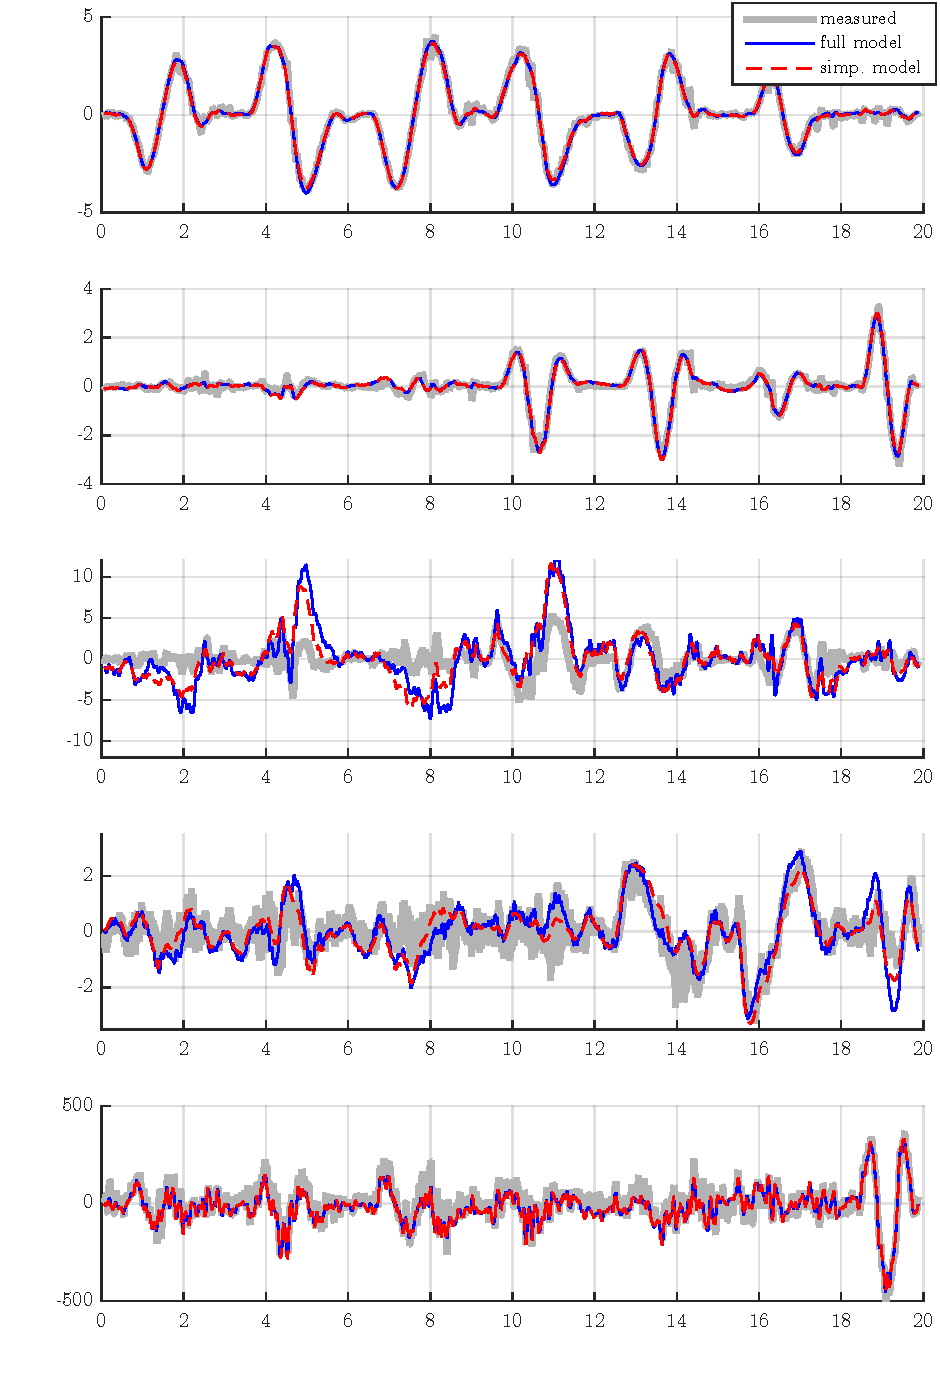
\includegraphics{ModelValidationTri.pdf}}%
\put(1.029882, 21.334540){\rotatebox{90}{\makebox(0,0)[t]{\smash{$\vxd$ in $\sfrac{\unit{m}}{\unit{s}^2}$}}}}%
\put(8.645781, 0.326348){\makebox(0,0)[b]{\smash{$t$ in $\unit{s}$}}}%
\put(0.677103, 2.890182){\rotatebox{90}{\makebox(0,0)[t]{\smash{$\PropVeld[1]$ in $\sfrac{\unit{RAD}}{\unit{s}^2}$}}}}%
\put(1.029882, 7.501271){\rotatebox{90}{\makebox(0,0)[t]{\smash{$\wzd$ in $\sfrac{\unit{RAD}}{\unit{s}^2}$}}}}%
\put(0.853493, 12.125590){\rotatebox{90}{\makebox(0,0)[t]{\smash{$\wyd$ in $\sfrac{\unit{RAD}}{\unit{s}^2}$}}}}%
\put(1.029882, 16.723451){\rotatebox{90}{\makebox(0,0)[t]{\smash{$\vzd$ in $\sfrac{\unit{m}}{\unit{s}^2}$}}}}%
\end{picture}%
\endgroup%
 \vspace{-20pt}
 \caption{Model vs. measured accelerations for the tricopter}
 \label{fig:ValidationTricopter}
\end{figure}

For the simplified model of the tricopter we drop all off diagonal entries in the system inertia matrix $\sysInertiaMat$.
This means in particular $\bodyCOM{}{}{} = 0$ and $\bodyMOI{}{}{} = \diag(\Jx, \Jy, \Jz)$.
Furthermore we drop the damping parameters $\lz=0$, $\sigx=\sigz=0$ and assume isotropic translational damping $D_v = \DampingSym \idMat[3]$ with $\DampingSym = \tfrac{1}{3}(2\dvx + \dvz)$.
The resulting model equations are summarized as follows:

\begin{RedBox}
\textbf{Simplified tricopter model.}
Rigid body dynamics
\begin{subequations}\label{eq:TricopterSimpModel}
\begin{align}
 \rd &= \R\, \v,&
 \m(\vd + \wedOp(\w)\v - \RT \gravityAcc) + \bodyDamping{}{} \v &= \F + \FB,
% \FBd &= 0,
\\
 \Rd &= \R \wedOp(\w),&
 \J \dot{\w} + \wedOp(\w) \J \w &= \tau + \tauB,
% \tauBd &= 0
\end{align}
Generalized force from propellers
\begin{align}\label{eq:TriActuatorTrafo}
 \underbrace{\begin{bmatrix}[1.2] \Fx \\ \Fy \\ \Fz \\ \taux \\ \tauy \\ \tauz \end{bmatrix}}_{\genForce}
 =
 \underbrace{\begin{bmatrix}[1.1] 
  0 & 0 & 0 & \tfrac{\sqrt{3}}{2} & 0 & -\tfrac{\sqrt{3}}{2} \\
  0 & 0 & 0 & -\tfrac{1}{2} & 1 & -\tfrac{1}{2} \\
  1 & 1 & 1 & 0 & 0 & 0 \\
   \tfrac{\sqrt{3}\,\ArmRadius}{2} & 0 & -\tfrac{\sqrt{3}\,\ArmRadius}{2} & \tfrac{\ArmHeight}{2} + \tfrac{\sqrt{3}\,\kappaT}{2\,\kappaF} & \ArmHeight & \tfrac{\ArmHeight}{2} + \tfrac{\sqrt{3}\,\kappaT}{2\,\kappaF} \\
  -\tfrac{\ArmRadius}{2} & \ArmRadius & -\tfrac{\ArmRadius}{2} & \tfrac{\sqrt{3}\,\ArmHeight}{2} - \tfrac{\kappaT}{2\,\kappaF} & \tfrac{\kappaT}{\kappaF} & \tfrac{\kappaT}{2\,\kappaF} - \tfrac{\sqrt{3}\,\ArmHeight}{2} \\
  \tfrac{\kappaT}{\kappaF} & -\tfrac{\kappaT}{\kappaF} & -\tfrac{\kappaT}{\kappaF} & -\ArmRadius & -\ArmRadius & -\ArmRadius
 \end{bmatrix}}_{B}
 \underbrace{\begin{bmatrix}[1.2] \F^{\mathsf{V}}_1 \\ \F^{\mathsf{V}}_2 \\ \F^{\mathsf{V}}_3 \\ \F^{\mathsf{H}}_1 \\ \F^{\mathsf{H}}_2 \\ \F^{\mathsf{H}}_3 \end{bmatrix}}_{\F^\mathsf{VH}}
\\
 \F^{\mathsf{V}}_j = \PropForce[j] \cos\aServo[j], 
 \quad
 \F^{\mathsf{H}}_j = \PropForce[j] \sin\aServo[j],
 \quad
 \PropForce[j] = \kappaF \PropVel[j]^2, \qquad j=1,2,3
\end{align}
Propeller drive dynamics
\begin{align}
 \PropInertia \PropVeld[j] + \kappaT \PropVel[j]^2 = \BLDCTorqueConstant[j] \BLDCCurr[j] - \BLDCFriction[j], \qquad j=1,2,3
% \PropVeld[j] + \PropParam[1] \PropVel[j]^2 = \PropParam[2] \BLDCCurr[j] - \PropParam[3], \qquad j=1,2,3.
\end{align}
Servo dynamics
\begin{align}\label{eq:TriModelServoDynamics}
 \aServodd[j] + \ServoParam[1] \aServod[j] + \ServoParam[0] \aServo[j] = \ServoParam[0] \aServoU[j], \qquad j=1,2,3
\end{align}

\end{subequations}
\end{RedBox}

Comparing the computed accelerations flight test in \autoref{fig:ValidationTricopter} one finds the following observations: % that the simplified model is as good or bad as the full model.
For the translational $\vxd$, $\vzd$ and the propeller acceleration $\PropVeld[1]$ the two models can not be distinguished and they match the measured accelerations quite well.
For the angular accelerations $\wxd$ and $\wzd$ the models differ slightly.
Unfortunately, one cannot say that the full model matches the measured accelerations better than the simplified.
This means that there are unmodeled effects that have a greater influence than the ones we dropped for the simplified model.
Overall the simplified model \eqref{eq:TricopterSimpModel} captures the Tricopter dynamics reasonably well and is due to its simplicity a good starting point for the model based control design.

\paragraph*{Quadcopter.}
As simplifications for the quadcopter model we neglect the inertial couplings between the center body and propeller except $\PropInertia \mat{H}_1 \PropVeld$.
Furthermore, we assume $\bodyCOM{}{}{} = 0$ and $\bodyMOI{}{}{} = \diag(\Jx, \Jx, \Jz)$.
The resulting model reads:

\begin{RedBox}
\textbf{Simplified quadcopter model.}
Rigid body dynamics
\begin{subequations}
\begin{align}
 \rd &= \R\, \v,&
 \m(\vd + \wedOp(\w)\v - \RT \gravityAcc) + \bodyDamping{}{} \v &= \Fz e_3 + \FB,
% \FBd &= 0,
\\
 \Rd &= \R \wedOp(\w),&
 \J \dot{\w} + \wedOp(\w) \J \w &= \tau + \tauB,
% \tauBd &= 0
\end{align}
Generalized force from propeller rotation
\begin{align}\label{eq:QuadActuatorTrafo}
 \begin{bmatrix} \Fz \\ \taux \\ \tauy \\ \tauz \end{bmatrix}
 =
 \underbrace{\begin{bmatrix}
  1 & 1 & 1 & 1 \\
  0 & \ArmRadius & 0 & -\ArmRadius \\
  -\ArmRadius & 0 & \ArmRadius & 0 \\
  -\tfrac{\kappaT}{\kappaF} & \tfrac{\kappaT}{\kappaF} & -\tfrac{\kappaT}{\kappaF} & \tfrac{\kappaT}{\kappaF} \\
 \end{bmatrix}}_{\mat{B}}
 \underbrace{\begin{bmatrix} \kappaF \PropVel[1]^2 \\ \kappaF \PropVel[2]^2 \\ \kappaF \PropVel[3]^2 \\ \kappaF \PropVel[4]^2 \end{bmatrix}}_{\tuple{\PropForce[]}}
 -
 \begin{bmatrix} 0 \\ 0 \\ 0 \\ \JP (\PropVeld[1] - \PropVeld[2] + \PropVeld[3] - \PropVeld[4]) \end{bmatrix}
\end{align}
Propeller drive dynamics
\begin{align}\label{eq:QuadPropDynamics}
 \PropInertia \PropVeld[j] + \kappaT \PropVel[j]^2 = \BLDCTorqueConstant[j] \BLDCCurr[j] - \BLDCFriction[j], \qquad j=1,\ldots,4.
\end{align}
\end{subequations}
\end{RedBox}

Up to a change in velocity coordinates this model is identical to the one proposed in \cite[eq.\ 7--12]{Mahony:Quadrotor2002}.

\begin{figure}[p]
 \centering
 \footnotesize%
 \appendtographicspath{{graphics/ModelValidationQuad/}}
 \begingroup%
\setlength{\unitlength}{1cm}%
\begin{picture}(15.900000,23.300000)%
\put(0,0){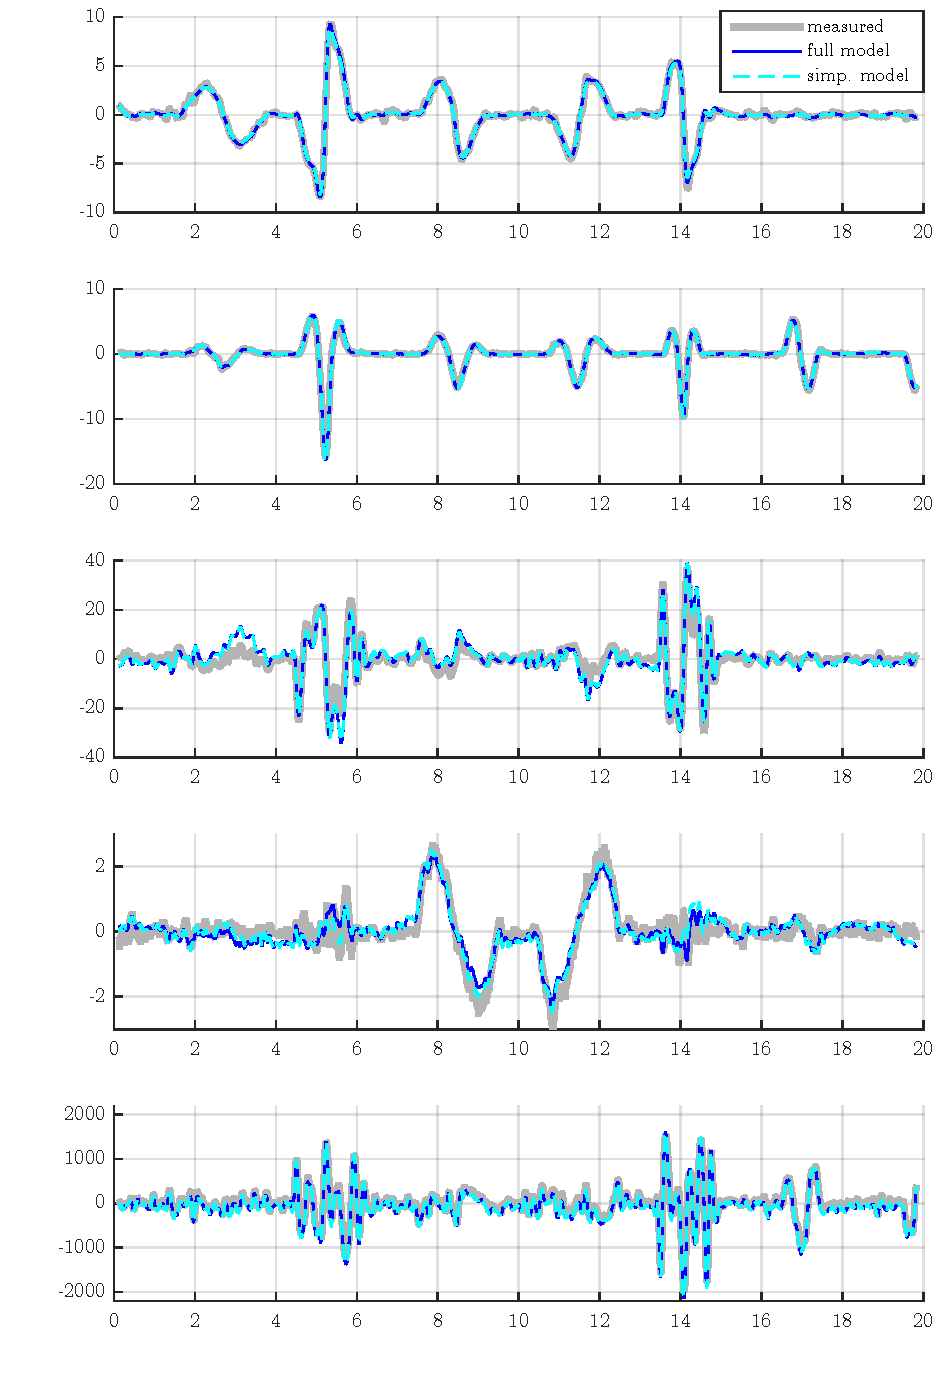
\includegraphics{ModelValidationQuad.pdf}}%
\put(0.710903, 7.501271){\rotatebox{90}{\makebox(0,0)[t]{\smash{$\wzd$ in $\sfrac{\unit{RAD}}{\unit{s}^2}$}}}}%
\put(8.750137, 0.326348){\makebox(0,0)[b]{\smash{$t$ in $\unit{s}$}}}%
\put(0.710903, 2.890182){\rotatebox{90}{\makebox(0,0)[t]{\smash{$\PropVeld[1]$ in $\sfrac{\unit{RAD}}{\unit{s}^2}$}}}}%
\put(0.710903, 12.125590){\rotatebox{90}{\makebox(0,0)[t]{\smash{$\wyd$ in $\sfrac{\unit{RAD}}{\unit{s}^2}$}}}}%
\put(0.710903, 16.723451){\rotatebox{90}{\makebox(0,0)[t]{\smash{$\vzd$ in $\sfrac{\unit{m}}{\unit{s}^2}$}}}}%
\put(0.710903, 21.334540){\rotatebox{90}{\makebox(0,0)[t]{\smash{$\vxd$ in $\sfrac{\unit{m}}{\unit{s}^2}$}}}}%
\end{picture}%
\endgroup%
 \vspace{-20pt}
 \caption{Model vs.\ measured accelerations on the quadcopter}
 \label{fig:ValidationQuadcopter}
\end{figure}

As discussed above for the tricopter, the validation result for the quadcopter is shown in \autoref{fig:ValidationQuadcopter} which is the first $20\,\unit{s}$ from \url{https://youtu.be/x66sua3M6RQ}.
The full model and simplified model can hardly be distinguished, so one may say that the simplifications are justified.
The measured translational accelerations and the propeller acceleration fit the model quite well.
For the angular accelerations there are slightly varying offsets between model and measurments.
These are probably aerodynamic disturbances rather than mechanical modeling errors.
Nevertheless, this motivates the use of a disturbance observer which will be discussed in a following section.

In contrast to the tricopter simplifications, the simplified quadcopter model did not drop the inertial coupling between the propellers and the yaw dynamics.
The reson for this is twofold:
The tricopter may generate yaw torque by tilting the propellers, whereas the quadcopter relies on the propeller drag and the inertial coupling, which are nominally much smaller.
Secondly, the experiments with the quadcopter perorm much more dynamic maneuvers which result in higher propeller accelerations as can be seen examplary by comparing \autoref{fig:ValidationQuadcopter} to \autoref{fig:ValidationTricopter}.

\section{Control of the generalized force}\label{sec:RealizationForceVectorControl}

\begin{enumerate}
 \item Servo simulation
 \item Propeller tracking control
 \item Tricopter force filter
 \item Quadcopter force filter
 \item reconstruction of the generalized force
\end{enumerate}


The rigid body controller computes a \textit{desired} generalised force $\genForceD$ for the corresponding multicopter.
Since the force $\genForce$ itself is subject to its own actuator dynamics (see \autoref{sec:RealizationModels}), it is not possible to realize it instantaneously.
However, we can pursue to realise it reasonably fast, which is the subject of this section.
At the same time we need an accurate estimate for the current generalized force for the rigid body observer.

\subsection{Servo simulation}
The integrated servo controller uses an internal angle measurement but this is not available for the main controller.
So for validation of the servo dynamics \eqref{eq:TriModelServoDynamics} and identification of its parameters $\ServoParam[0]$ and $\ServoParam[1] $, a dedicated test bench with an incremental encoder for the tilt angle $\aServo$ was used.
Since the model is asymptotically stable a simple online simulation of the model is sufficient to get an estimate of the current servo angle.
For this a simple forward Euler discretization of \eqref{eq:TriModelServoDynamics} is implemented on the main controller
\begin{subequations}\label{eq:ServoSimulator}
\begin{align}
 \aServoObs[][k\!+\!1] &= \aServoObs[][k] + \Ts \aServoObsd[][k]
\\
 \aServoObsd[][k\!+\!1] &= \aServoObsd[][k] + \Ts( \ServoParam[0] (\aServoU[][k] - \aServoObs[][k]) - \ServoParam[1] \aServoObsd[][k])
 .
\end{align}
\end{subequations}
% \fixme{Servo param}
% \begin{align}
%  p_{\textsf{S}0} = \tfrac{K_P}{\ArmInertia}, \
%  p_{\textsf{S}1} = \tfrac{K_D}{\ArmInertia}
% \end{align}
In \autoref{fig:ServoSimRes} its result is compared to the measurement of the encoder.
To be close to the real application on the Tricopter, the propeller on the test bench is spinning with about $70\,\unit{Hz}$ during the experiment.
This explains the vibration seen in the encoder measurements.
If the propeller is switched off, the estimation error is always less than $\pm 0.5\,\unit{DEG}$.

\begin{figure}
 \centering
 \footnotesize
 \appendtographicspath{{graphics/ServoSimRes/}}
 \begingroup%
\setlength{\unitlength}{1cm}%
\begin{picture}(15.900000,10.000000)%
\put(0,0){\includegraphics{ServoSimRes.pdf}}%
\put(0.824791, 2.272028){\rotatebox{90}{\makebox(0,0)[t]{\smash{error in $\unit{RAD}$}}}}%
\put(0.648402, 6.999183){\rotatebox{90}{\makebox(0,0)[t]{\smash{$\aServo$ in $\unit{RAD}$}}}}%
\end{picture}%
\endgroup%
 \caption{Servo simulation validation}
 \label{fig:ServoSimRes}
\end{figure}

\subsection{Propeller tracking control}
The forward Euler discretization of the propeller model \eqref{eq:QuadPropDynamics} is
\begin{align}\label{eq:PropDynamics}
 \PropVel[][k\!+\!1] = \PropVel[][k] + \Ts \big( \PropParam[2] \BLDCCurr[][k] - \PropParam[3] - \PropParam[1] \big( \PropVel[][k]\big)^2 \big),
\end{align}

\paragraph*{Measurement model.}
From the commutation algorithm of the BLDC driver we get an estimate $\PropVelMeas$ of the propeller velocity which relies on its \textit{angle} $\PropAngle$ estimation used for the commutation, which is
\begin{align}
 \PropVelMeas[][k] = \tfrac{1}{\Ts} \big( \PropAngle[][k] - \PropAngle[][k\!-\!1] \big)
 .
\end{align} 
Assuming that the angular acceleration $\PropVeld$ is roughly constant within one sampling step, we have the relations
\begin{align}
 \PropAngle[][k] = \PropAngle[][k\!-\!1] + \PropVel[][k\!-\!1] \Ts + \tfrac{1}{2} \PropVeld[][k\!-\!1] \Ts^2,
\quad
 \PropVeld[][k\!-\!1] = \tfrac{1}{\Ts} \big( \PropVel[][k] - \PropVel[][k\!-\!1] \big)
 .
\end{align}
So the estimate corresponds to the mean velocity between the current and the last sampling step, \ie
\begin{align}\label{eq:PropMeaseq}
 \PropVelMeas[][k] = \tfrac{1}{2} \big( \PropVel[][k] + \PropVel[][k\!-\!1] \big)
 .
\end{align} 

\paragraph*{Observer.}
The velocity estimate $\PropVelMeas$ from the BLDC driver is quite noisy, so it should not be used directly in a feedback.
The scaled model \eqref{eq:PropDynamics} also contains the a friction parameter $\PropParam[3] = \tfrac{\BLDCFriction}{\PropInertia}$ which we like to estimate online for each propeller drive individually.
To address these two aspects, an observer for each propeller drive is implemented on the main controller.
It is essentially a copy of the discrete model \eqref{eq:PropDynamics} supplemented with a linear error feedback
\begin{subequations}\label{eq:PropObserver}
\begin{align}
 e[k] &= \PropVelMeas[][k] - \tfrac{1}{2} \big( \PropVelObs[][k] + \PropVelObs[][k-1] \big)
\\
 \PropVelObs[][k+1] &= \PropVelObs[][k] + \Ts \big( \PropParam[2] \BLDCCurr[][k] - \PropParamObs[3][k] - \PropParam[1] \big( \PropVelObs[][k]\big)^2 + \PropObsGainVel e[k] \big),
\\
 \PropParamObs[3][k+1] &= \PropParamObs[3][k] + \Ts \PropObsGainBias e[k].
\end{align}
\end{subequations}
where $\PropObsGainVel, \PropObsGainBias \in \RealNum$ are the feedback gains.
For quantitative analysis of the observer we consider the linearization of the observer error dynamics about a general expansion point $\PropVel = \PropVelStat > 0$.
Its characteristic polynomial is
\begin{align}
 \lambda^3 
 + \big( \tfrac{\Ts}{2} \big( 4 \PropParam[1] \PropVelStat + \PropObsGainVel \big) - 2 \big) \lambda^2
 + \big( 1 - \tfrac{\Ts}{2} \big( 4 \PropParam[1] \PropVelStat + \Ts \PropObsGainBias \big) \big) \lambda
 - \tfrac{\Ts}{2} \big( \PropObsGainVel + \Ts \PropObsGainBias \big)
 = 0
\end{align}
The roots $\lambda$ for the given parameters are shown in (??).

% \begin{subequations}
% \begin{align}
%  a_0 &= -\tfrac{\Ts}{2} \big( \PropObsGainVel + \Ts \PropObsGainBias \big),
% \\
%  a_1 &= 1 - \tfrac{\Ts}{2} \big( 4 \PropParam[1] \PropVelStat + \Ts \PropObsGainBias \big),
% \\
%  a_2 &= \tfrac{\Ts}{2} \big( 4 \PropParam[1] \PropVelStat + \PropObsGainVel \big) - 2,
% \\
%  a_3 &= 1.
% \end{align}
% \end{subequations}

\paragraph*{Tracking controller.}
Assume that we have a given trajectory $k \mapsto \PropVelDF[][k]$ and we want the trajectory of the propeller velocity $k \mapsto \PropVel[][k]$ (actually its estimate $\PropVelObs$) to converge to it.
Being at the sampling step $k$ the available control input is the motor current $\BLDCCurr[][k\!+\!1]$ for the \textit{next} step.
From the observer \eqref{eq:PropObserver} we have estimates for the velocity $\PropVelObs[][k\!+\!1]$ and the friction $\PropParamObs[3][k\!+\!1]$ at the next sampling step.
Taking this into account we propose the control law:
\begin{subequations}\label{PropCtrlLaw}
\begin{align}
 e[k\!+\!1] &= \PropVelDF[][k\!+\!1] - \PropVelObs[][k\!+\!1],
\\
 \BLDCCurr[][k\!+\!1] &= \tfrac{1}{\PropParam[2]} \big( \tfrac{\PropVelDF[][k+2] - \PropVelDF[][k+1]}{\Ts} + \PropParam[1] \big( \PropVelDF[][k\!+\!1] \big)^2 + \PropParamObs[3][k\!+\!1] + \PropCtrlGain e[k\!+\!1] \big),
\end{align}
\end{subequations}
It is essentially a (shifted) copy of the discrete model \eqref{eq:PropDynamics} supplemented with a linear error feedback with the gain $\PropCtrlGain \in \RealNum$.
Plugging the control law \eqref{PropCtrlLaw} into the model \eqref{eq:PropDynamics} and assuming the observer has converged, \ie $\PropVelObs[][k] = \PropVel[][k]$ and $\PropParamObs[3][k] = \PropParam[3]$, yields the tracking error dynamics
\begin{align}
 e[k\!+\!1] + \big( \Ts (2 \PropParam[1] \PropVel[][k] + \PropCtrlGain) - 1 \big) e[k] + \Ts \PropParam[1] \big( e[k] \big)^2 = 0.
\end{align}
For a the linearization about the expansion point $e = 0$, $\PropVel = \PropVelStat$ the corresponding characteristic polynomial has the root
\begin{align}
 \lambda = 1 - \Ts (2 \PropParam[1] \PropVelStat + \PropCtrlGain).
\end{align}


\begin{figure}
 \centering
 \footnotesize
 \appendtographicspath{{graphics/PropCtrlRes/}}
 \begingroup%
\setlength{\unitlength}{1cm}%
\begin{picture}(15.900000,17.000000)%
\put(0,0){\includegraphics{PropCtrlRes.pdf}}%
\put(0.980045, 8.981390){\rotatebox{90}{\makebox(0,0)[t]{\smash{error in $\unit{N}$}}}}%
\put(1.372021, 13.880619){\rotatebox{90}{\makebox(0,0)[t]{\smash{$\PropForce$ in $\unit{N}$}}}}%
\put(8.830640, 0.302626){\makebox(0,0)[b]{\smash{$t$ in $\unit{s}$}}}%
\put(0.744859, 2.363751){\rotatebox{90}{\makebox(0,0)[t]{\smash{$\hat{\tau}_{\mathsf{MB}}$ in $\unit{Nm}$}}}}%
\put(1.195632, 5.665956){\rotatebox{90}{\makebox(0,0)[t]{\smash{$\BLDCCurr$ in $\unit{A}$}}}}%
\end{picture}%
\endgroup%
 \caption{Propeller control validation}
 \label{fig:PropCtrlRes}
\end{figure}

\subsection{Tricopter force control}
The generalized force $\genForce$ on the \Tricopter is a static transformation of the propeller velocities $\PropVel[1], \ldots \PropVel[3]$ and the servo angles $\aServo[1],\ldots,\aServo[3]$ as given in \eqref{eq:TriActuatorTrafo}.
For a given desired generalized force $\genForceD$ we can (partially) invert this relation to obtain the corresponding propeller thrusts $\PropForceD[1], \ldots \PropForceD[3]$ and servo angles $\aServoD[1],\ldots,\aServoD[3]$ as
\begin{align}\label{eq:TriInvActuatorTrafo}
 \F_{\idxDes}^\mathsf{VH} = B^{-1} \genForceD,
\quad
 \PropForceD[j] = \sqrt{(\F_{\idxDes j}^\mathsf{V})^2 + (\F_{\idxDes j}^\mathsf{H})^2},
\quad
 \aServoD[j] = \atanTwo(\F_{\idxDes j}^\mathsf{H}, \F_{\idxDes j}^\mathsf{V}),
\quad j = 1,2,3.
\end{align}
In addition the computed values are saturated to $0.3\,\unit{N} \leq \PropForceD[i] \leq 7.0\,\unit{N}$ and $-45^\circ\leq \aServoD[i] \leq 45^\circ, i=1,2,3$ to incorporate the practical limitations of the actuators.
The desired servo angles $\aServoD[i]$ are directly forwarded to the servo controllers.
In contrast, for the desired thrusts $\PropForce[i]$ a first order filter is applied:
\begin{align}\label{eq:PropPrefilter}
 \PropForceDF[][k\!+\!2] = \lambda_{\mathsf{Filt}} \PropForceDF[][k\!+\!1] + (1-\lambda_{\mathsf{Filt}}) \PropForceD[][k\!+\!1],
\qquad
 \PropVelDF[][k\!+\!2] = \sqrt{\sfrac{\PropForceDF[][k\!+\!2]}{\kappaF}}.
\end{align}
This yields the desired propeller velocities $\PropVelDF[i][k+1]$ and $\PropVelDF[i][k+2]$ for the next \textit{two} sampling steps which are required for the propeller \textit{tracking} controller.
After the propeller controller has converged, \ie $\PropForce[i] = \PropForceDF[i]$, the thrust dynamic is completely determined by this filter.

Overall we can combine the discrete servo dynamics \eqref{eq:ServoSimulator}, the thrust filter \eqref{eq:PropPrefilter} and the static transformations \eqref{eq:TriActuatorTrafo} and \eqref{eq:TriInvActuatorTrafo} to obtain a nonlinear dynamic system with the input $\genForceD$ and the output $\genForce$, the \textit{\Tricopter actuator dynamics}.
For a quantitative analysis its first order approximation about a general expansion point $(\PropForceStat[1], \PropForceStat[2], \PropForceStat[3], \aServoStat[1], \aServoStat[2], \aServoStat[3])$ is considered.
Using the $z$-transformation $\ZTrafo{\cdot}$ the linearized dynamics between $\genForce$ and $\genForceD$ can be written as 
\begin{align}
 \ZTrafo{\Delta \genForce} = \GenForceTransferFunction(z) \, \ZTrafo{\Delta \genForceD}.
\end{align}
The discrete transfer function
\begin{align}\label{eq:TriActuatorTransferFunction}
 \GenForceTransferFunction(z) = J \diag(\ThrustTransferFunction(z), \ThrustTransferFunction(z), \ThrustTransferFunction(z), \ServoTransferFunction(z), \ServoTransferFunction(z), \ServoTransferFunction(z)) J^{-1}
\end{align}
consists of $\ThrustTransferFunction(z)$, the transfer function of the thrust filter \eqref{eq:PropPrefilter}, $\ServoTransferFunction(z)$, the transfer function of the controlled servo \eqref{eq:ServoSimulator}:
\begin{align}
 \ThrustTransferFunction(z) = \frac{1-c_F}{z-c_F},
\qquad
 \ServoTransferFunction(z) = \frac{\ServoParam[0] \Ts^2}{(z-1)^2 + \ServoParam[1]\Ts (z-1) + \ServoParam[0] \Ts^2}
 .
\end{align}
and $J$ is the Jacobian matrix of the force transformation \eqref{eq:TriActuatorTrafo} at the expansion point.
\begin{align}
 %\underbrace{\begin{bmatrix} \Delta \Fx \\ \Delta \Fy \\ \Delta \Fz \\ \Delta \taux \\ \Delta \tauy \\ \Delta \tauz \end{bmatrix}}_{\Delta \genForce}
 J = B
 \begin{bmatrix}
  \cos\aServoStat[1] & 0 & 0 & -\PropForceStat[1] \sin\aServoStat[1] & 0 & 0 \\
  0 & \cos\aServoStat[2] & 0 & 0 & -\PropForceStat[2] \sin\aServoStat[2] & 0 \\
  0 & 0 & \cos\aServoStat[3] & 0 & 0 & -\PropForceStat[3] \sin\aServoStat[3] \\
  \sin\aServoStat[1] & 0 & 0 & \PropForceStat[1] \cos\aServoStat[1] & 0 & 0 \\
  0 & \sin\aServoStat[2] & 0 & 0 & \PropForceStat[2] \cos\aServoStat[2] & 0 \\
  0 & 0 & \sin\aServoStat[3] & 0 & 0 & \PropForceStat[3] \cos\aServoStat[3] \\
 \end{bmatrix}
% \begin{bmatrix} \Delta \PropForce[1] \\ \Delta \PropForce[2] \\ \Delta \PropForce[3] \\ \Delta \aServo[1] \\ \Delta \aServo[2] \\ \Delta \aServo[3] \end{bmatrix}
 .
\end{align}
Note that $\PropForceStat$ cancels out in \eqref{eq:TriActuatorTransferFunction}, \ie $\GenForceTransferFunction$ is independent of it.

From the structure of $\GenForceTransferFunction$ in \eqref{eq:TriActuatorTransferFunction} it is clear that its entries are linear combinations of the transfer functions the the thrust and the servos, $\ThrustTransferFunction$ and $\ServoTransferFunction$.
Also it is evident that if $\ThrustTransferFunction = \ServoTransferFunction$, then $\GenForceTransferFunction$ would be diagonal.
Since this is not the case we do have off-diagonal entries in the transfer matrix $\GenForceTransferFunction$.
This so-called crosstalk between the components of the generalized force $\genForce$ depends mainly on the expansion point of the servo angles $\aServoStat$.

For a better quantitative analysis of the off-diagonal entries of $\GenForceTransferFunction$, the transfer function is normalized as $\GenForceTransferFunctionNorm = S^{-1} \GenForceTransferFunction S $ where $S = \diag(F_{\mathsf{x,Max}}, \ldots, \tau_{\mathsf{z,Max}})$ contains the maximal magnitudes of the corresponding forces and torques.
\autoref{fig:BodeTriActorDyn} shows exemplary the bode magnitude plot of $\GenForceTransferFunctionNorm$ for the hover case $\aServoStat = [0,0,0]^\top$ (left) and for a forward force with $\aServoStat = [\sfrac{\pi}{4},0,-\sfrac{\pi}{4}]^\top$ (right).
In the hover case the diagonal entries for $\Fz$, $\taux$ and $\tauy$ coincide with the thrust dynamics $\ThrustTransferFunction$, whereas the diagonal entries for $\Fx$ and $\Fy$ coincide with the servo dynamics $\ServoTransferFunction$.
The diagonal entry for $\tauz$ is dominated by the servo dynamics $\ServoTransferFunction$ but also has a small influence from $\ThrustTransferFunction$ due to the propeller drag (terms involving $\kappaT$ in \eqref{eq:TriActuatorTrafo}).
The propeller drag is also responsible for the small off-diagonal entries in the hover case.
For the forward force case it is evident that the diagonal entries are linear combinations of $\ThrustTransferFunction$ and $\ServoTransferFunction$.
Furthermore, the off-diagonal entries have a significantly larger magnitude.

\begin{figure}
 \centering
 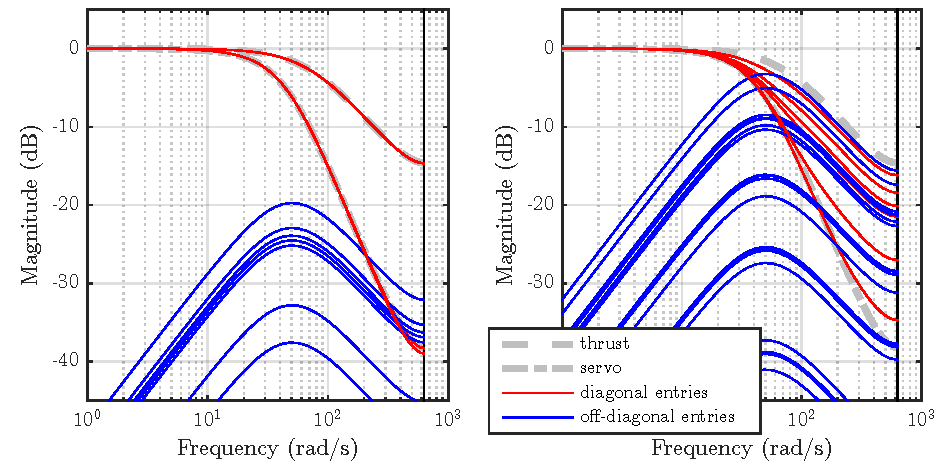
\includegraphics{graphics/TriActuatorDynamics/BodeTriActorDyn.pdf}
 \caption{Bode magnitude plot of the normalized \Tricopter actuator dynamics transfer function $\GenForceTransferFunctionNorm$ at different expansion points}
 \label{fig:BodeTriActorDyn}
\end{figure}


% \begin{figure}[htb]
%  \centering
%  \input{graphics/PropCtrlBlock.pdf_tex}
%  \caption{Structure of the Propeller control algorithm}
%  \label{fig:PropCtrlBlock}
% \end{figure}


\subsection{Quadcopter force vector control}
\paragraph{Model.}
The model of the generalized force on the quadcopter from \eqref{eq:QuadActuatorTrafo} can be split into a static part $\genForceQuadStat$, proportional to the squares of the propeller velocities $\PropVel$, and a dynamic part $\genForceQuadDyn$ proportional to the propeller accelerations $\PropVeld$, as
\begin{align}\label{eq:QuadForceVelctorModel}
% \underbrace{\begin{bmatrix} \Fz \\ \taux \\ \tauy \\ \tauz \end{bmatrix}}_{\genForceQuad}
 \genForceQuad(\PropVel, \PropVeld)
 =
 \underbrace{
 \overbrace{\begin{bmatrix}
  \kappaF & \kappaF & \kappaF & \kappaF \\
  0 & \kappaF\ArmRadius & 0 & -\kappaF\ArmRadius \\
  -\kappaF\ArmRadius & 0 & \kappaF\ArmRadius & 0 \\
  -\kappaT & \kappaT & -\kappaT & \kappaT \\
 \end{bmatrix}}^{B}
 %\underbrace{
 \begin{bmatrix} \PropVel[1]^2 \\ \PropVel[2]^2 \\ \PropVel[3]^2 \\ \PropVel[4]^2 \end{bmatrix}
 %}_{\PropForce[]}
 }_{\genForceQuadStat(\PropVel)}
 -
 \underbrace{\begin{bmatrix} 0 \\ 0 \\ 0 \\ \JP (\PropVeld[1] - \PropVeld[2] + \PropVeld[3] - \PropVeld[4]) \end{bmatrix}}_{\genForceQuadDyn(\PropVeld)}
 .
\end{align}

\paragraph{Filter dynamics.}
The task here is to design a filter which outputs the desired propeller velocities $\PropVel[][k]$ and $\PropVel[][k+1]$ for the next two sampling steps based on the given desired generalized force $\genForceQuadD[k]$.
Note that $\genForceQuad$ is \textit{not} a flat output of \eqref{eq:QuadForceVelctorModel}, so a simple low-pass filter for $\genForceQuadD$ does not do the trick.
However, the propeller velocities $\PropVel$ form a flat output and so we propose the following continuous time filter
\begin{align}\label{eq:QuadActuatorFilterDesign}
 \tfrac{\d^2}{\d t^2} \big(\genForceQuadStat(\PropVelDF)\big) + K_1 \tfrac{\d}{\d t} \big(\genForceQuadStat(\PropVelDF)\big) + K_0 \big( \genForceQuad(\PropVelDF,\PropVelDFd) - \genForceQuadD \big) = 0
 .
\end{align}
With introduction of the auxiliary state $\hat{h} = \tfrac{\d}{\d t} \big(\genForceQuadStat(\PropVelDF)\big) + K_1 \genForceQuadStat(\PropVelDF)$ this can be rewritten in an explicit first order form
\begin{subequations}\label{eq:QuadcopterActuatorFilter}
\begin{align}
 \PropVelDFd &= \diag(2 \kappaF \PropVelDF)^{-1} B^{-1} \big( \hat{h} - K_1 \genForceQuadStat(\PropVelDF) \big),
\\
 \dot{\hat{h}} &= K_0 \big( \genForceQuadD - \genForceQuad(\PropVelDF,\PropVelDFd) \big).
\end{align}
\end{subequations}
For the time discrete implementation we add the forward Euler approximation of the derivatives
\begin{align}\label{eq:QuadcopterActuatorFilterDiscretization}
 \PropVelDF[][k\!+\!1] = \PropVelDF[][k] + \Ts \PropVelDFd[][k],
\qquad
 \hat{h}[k\!+\!1] = \hat{h}[k] + \Ts \dot{\hat{h}}[k].
\end{align}
With this representation of the filter dynamics it is very simple to add a saturation $\PropVelMin \leq \PropVelDF \leq \PropVelMax$ to take into account the practical limitations of the propellers.
The combination of \eqref{eq:QuadcopterActuatorFilter} and \eqref{eq:QuadcopterActuatorFilterDiscretization} constitute a time discrete nonlinear system with the input $\genForceQuadD[k]$ and the output $\PropVelDF[][k]$, $\PropVelDF[][k+1]$, the \textit{quadcopter actuator dynamics}.  

\paragraph{Tuning.}
The filter gains $K_1$ and $K_2$ are chosen as diagonal matrices and for symmetry considerations the gains corresponding to $\taux$ and $\tauy$ are identical, \ie
\begin{align}
 K_0 = \diag(\kPMag, \kPTilt, \kPTilt, \kPHead),
\qquad
 K_1 = \diag(\kDMag, \kDTilt, \kDTilt, \kDHead).
\end{align}
For a quantitative analysis of the actuator dynamics we consider its linearization for a general expansion point $(\PropVelStat[1], \ldots, \PropVelStat[4]) \in [\PropVelMin, \PropVelMax]^4$.
Using the $z$-transformation we get the following transfer matrix 
\begin{align}
 \ZTrafo{\Delta \genForce} = \GenForceTransferFunction(z) \, \ZTrafo{\Delta \genForceD},
\qquad
 \GenForceTransferFunction(z) =
 \begin{bmatrix}
  G_{11}(z) & 0 & 0 & 0 \\
  0 & G_{22}(z) & 0 & 0 \\
  0 & 0 & G_{33}(z) & 0 \\
  G_{41}(z) & G_{42}(z) & G_{43}(z) & G_{44}(z) \\
 \end{bmatrix}
\end{align}
with the components
\begin{subequations}\label{eq:QuadActuatorDynTransferComponents}
\begin{align}
% G_{11}(z) &= \frac{\kPMag\Ts^2}{(z-1)^2 + \kDMag\Ts (z-1) + \kPMag\Ts^2}
 G_{11}(z) &= \frac{\kPMag}{\big(\tfrac{z-1}{\Ts}\big)^2 + \kDMag \tfrac{z-1}{\Ts} + \kPMag}
\\
 G_{22}(z) = G_{33}(z) &= \frac{\kPTilt}{\big(\tfrac{z-1}{\Ts}\big)^2 + \kDTilt \tfrac{z-1}{\Ts} + \kPTilt}
\\
 G_{44}(z) &= \frac{\kPHead(p_4\tfrac{z-1}{\Ts} + 1)}{\big(\tfrac{z-1}{\Ts}\big)^2 + (\kPHead p_4 + \kDTilt) \tfrac{z-1}{\Ts} + \kPHead}
\\
 G_{4j}(z) &= \frac{p_j\,G_{jj}(z)\,\big(\tfrac{z-1}{\Ts}\big)^2 (\tfrac{z-1}{\Ts} + \kDHead)}{\big(\tfrac{z-1}{\Ts}\big)^2 + (\kPHead p_4 + \kDTilt) \tfrac{z-1}{\Ts} + \kPHead}, \quad j=1,2,3
\end{align}
\end{subequations}
and the (expansion point dependent) model parameters
\begin{subequations}
\begin{align}
 p_1 &= \tfrac{\PropInertia}{8\kappaF} \left( \tfrac{1}{\PropVelStat[4]} - \tfrac{1}{\PropVelStat[3]} + \tfrac{1}{\PropVelStat[2]} - \tfrac{1}{\PropVelStat[1]} \right),&
 p_2 &= \tfrac{\PropInertia}{4\kappaF\ArmRadius} \left( \tfrac{1}{\PropVelStat[2]} - \tfrac{1}{\PropVelStat[4]} \right),
\\
 p_4 &= \tfrac{\PropInertia}{8\kappaT} \left( \tfrac{1}{\PropVelStat[1]} + \tfrac{1}{\PropVelStat[2]} + \tfrac{1}{\PropVelStat[3]} + \tfrac{1}{\PropVelStat[4]} \right),&
 p_3 &= \tfrac{\PropInertia}{4\kappaF\ArmRadius} \left( \tfrac{1}{\PropVelStat[1]} - \tfrac{1}{\PropVelStat[3]} \right).
\end{align}
\end{subequations}
The transfer behaviors for $\Fz$, $\taux$ and $\tauy$ are uncorrelated and independent of the expansion point.
Their parameters are chosen to form a second order Butterworth filter.

Unfortunately, the transfer behavior for $\tauz$ is not that nice:
It is in general affected by all components of $\genForceD$ and the corresponding transfer functions $G_{4j}, j=1,\ldots,4$ depend on the expansion point.
However, for the hover case $\PropVelStat[1] = \PropVelStat[2] = \PropVelStat[3] = \PropVelStat[4] = \sqrt{\sfrac{m \gravityAccConst}{4\kappaF}}$ we have $p_1=p_2=p_3=0$ and $p_4 = \tfrac{\PropInertia}{\kappaT}\sqrt{\sfrac{\kappaF}{m \gravityAccConst}}$.
We choose $\kDHead = \sfrac{1}{p_4} = \tfrac{\kappaT}{\PropInertia}\sqrt{\sfrac{m \gravityAccConst}{\kappaF}}$ such that \textit{at this particular expansion point} we have a pole-zero cancellation.
The remaining parameter $\kPHead$ is then used to adjust the cut-off frequency of the filter.

\autoref{fig:BodeQuadActorDyn} shows the Bode magnitude plot of the normalized transfer matrix $\GenForceTransferFunctionNorm$ coefficients from \eqref{eq:QuadActuatorDynTransferComponents} with the used filter parameters.
The left side corresponds to the most common hover case $\PropVelStat[1] = \PropVelStat[2] = \PropVelStat[3] = \PropVelStat[4] = \sqrt{\sfrac{m \gravityAccConst}{4\kappaF}}$ whereas the right side captures the ``worst case`` expansion points where $(\PropVelStat[1], \ldots,\PropVelStat[4]) \in \{ \PropVelMin, \PropVelMax\}^4$.
Obviously the pole-zero cancellation only holds for the hover case but even for the worst case points $G_{44}$ only differs slightly from its design.
Furthermore one can see that the influence of the off-diagonal entries is restricted to high frequencies.

\begin{figure}[ht]
 \centering
 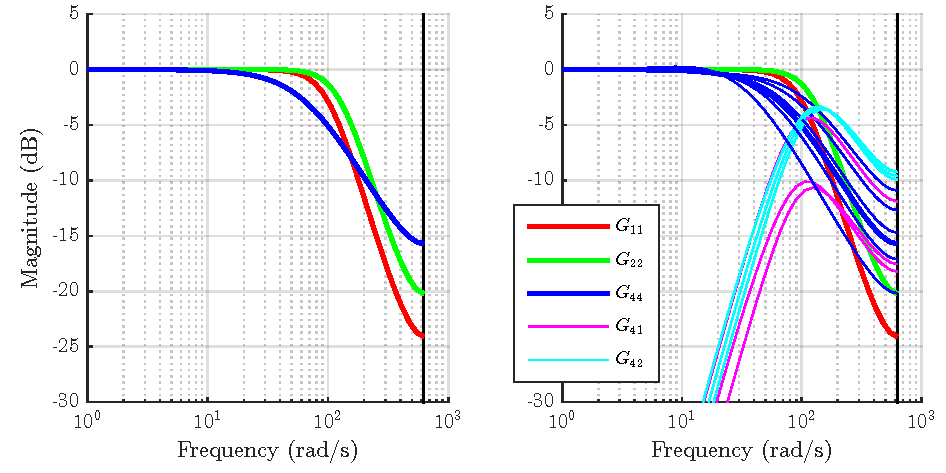
\includegraphics{graphics/QuadActuatorDynamics/BodeQuadActorDyn.pdf}
 \caption{Bode magnitude plot of the normalized transfer matrix $\GenForceTransferFunctionNorm$ at different expansion points}
 \label{fig:BodeQuadActorDyn}
\end{figure}

\paragraph{Comparison to static approach.}
The proposed filter \eqref{eq:QuadActuatorFilterDesign} might seem complicated.
In particular one might argue that the dynamic part $\genForceQuadDyn$ in the model \eqref{eq:QuadForceVelctorModel} is neglectable, as is done in most publications on this subject.

To answer this question we can replace \eqref{eq:QuadActuatorFilterDesign} by
\begin{align}\label{eq:QuadActuatorFilterDesignTraditional}
 \tfrac{\d^2}{\d t^2} \big(\genForceQuadStat(\PropVelDF)\big) + K_1 \tfrac{\d}{\d t} \big(\genForceQuadStat(\PropVelDF)\big) + K_0 \big( \genForceQuadStat(\PropVelDF) - \genForceQuadD \big) = 0
\end{align}
what essentially neglects the dynamics part $\genForceQuadDyn$ in the generalized force $\genForceQuad = \genForceQuadStat + \genForceQuadDyn$.
As before we now consider the transfer matrix $\GenForceTransferFunction$ for the linearized filter at a general expansion point.
The components differing from \eqref{eq:QuadActuatorDynTransferComponents} are
\begin{align}\label{eq:QuadActuatorDynTransferTraditionalComponents}
 G_{44}(z) = \frac{\kPHead(p_4\tfrac{z-1}{\Ts} + 1)}{\big(\tfrac{z-1}{\Ts}\big)^2 + \kDTilt \tfrac{z-1}{\Ts} + \kPHead}
\qquad
 G_{4j}(z) = p_j\,\tfrac{z-1}{\Ts}\,G_{jj}(z), \ j=1,2,3.
\end{align}
Now one can chose the gains $K_0$ and $K_1$ such that \eqref{eq:QuadActuatorFilterDesignTraditional} forms 4 decoupled second order Butterworth filters with inputs $\genForceQuadD$ and outputs $\genForceQuadStat$.
However, since the real force on the quadcopter does contain the dynamic part as well the behavior from $\genForceQuadD$ to $\genForceQuad = \genForceQuadStat + \genForceQuadDyn$ is quite different, as can be seen in \eqref{eq:QuadActuatorDynTransferTraditionalComponents}.
The Bode magnitude plot of the transfer functions is displayed in \autoref{fig:BodeQuadActorDynTraditional} on the left side.
Even for the hover case (thick lines) the transfer function $G_{44}$ for $\tauz$ has an unacceptable overshot.

In oder to improve the behavior we can do the same as before: adjust the parameters in $G_{44}$, \ie $\kPHead$ and $\kDHead$, such that there is a pole-zero cancelation at the hover expansion point.
The resulting Bode magnitude plot is shown on the right side of \autoref{fig:BodeQuadActorDynTraditional}.
It is already a significant improvement compared to the right side but is much worse as the previous result shown in \autoref{fig:BodeQuadActorDyn}.
Moreover, the magnitude of the off-diagonal transfer functions at low frequencies is much higher for both cases in \autoref{fig:BodeQuadActorDynTraditional} than in \autoref{fig:BodeQuadActorDyn}.

\begin{figure}[ht]
 \centering
 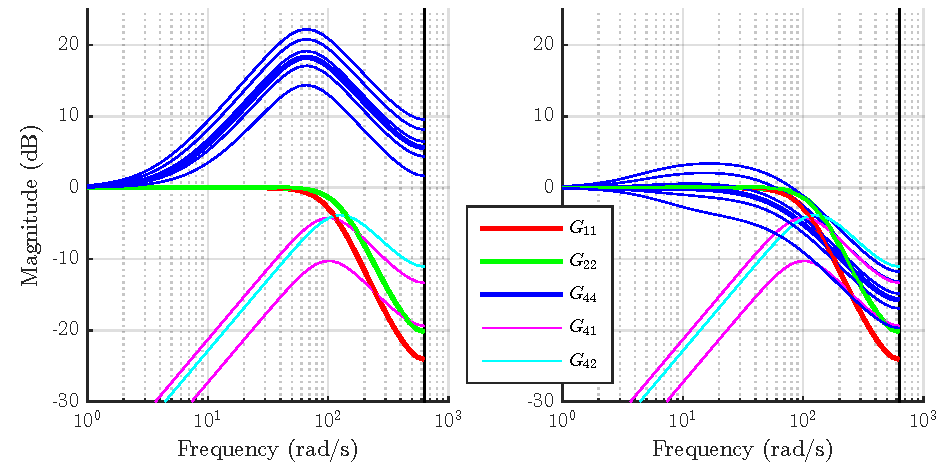
\includegraphics{graphics/QuadActuatorDynamics/BodeQuadActorDynTraditional.pdf}
 \caption{Bode magnitude plot of the normalized transfer matrix $\GenForceTransferFunctionNorm$ at different expansion points (static approach)}
 \label{fig:BodeQuadActorDynTraditional}
\end{figure}

Overall this discussion should justify the filter design in \eqref{eq:QuadActuatorFilterDesign} and justify the consideration of the dynamic model \eqref{eq:QuadForceVelctorModel} for the present case.
For other quadcopters with smaller ratios $\sfrac{\PropInertia}{\kappaT}$ or less aggressively tuned multicopters like the previously discussed tricopter, however, the situation can be different.


% \subsection{Propeller aerodynamics}
% picture of the propeller, its geometric center and the forces
% 
% The main purpose of a propeller is to generate a force $\vect{F} = \PropForce \,\vect{b}_3$ in its spinning direction $\vect{b}_3$, but the actual aerodynamics contain several mode effects.
% 
% \paragraph{Aerodynamic model.}
% In the following we discuss the propeller model proposed in \cite{Martin:AccelerometerFeedback}.
% They claim that it is based on general blade element theory from \cite{Johnson:HelicopterTheory}, but is adopted to the specific conditions of their quadcopter which is about the same size as the one build for this work. 
% The proposed model is\footnote{There is probably a typo in \cite{Martin:AccelerometerFeedback}, eq.\ (2), the definition is corrected such that their result in eq.\ (7) is plausible.}
% \begin{subequations}\label{eq:PropellerForceTorque}
% \begin{alignat}{10}
% %  \vect{F} & \ = \ &
% %  \kappa_F &\PropVel^2 \vect{b}_3&
% %  \ &- \ &
% %  &\PropVel ( \lambda_1 \vect{v}^\bot + \lambda_2 \vect{\omega} \times \vect{b}_3 )&
% %  \ &- \ &
% %  \PropDir &\PropVel (\lambda_3 \vect{v} \times \vect{b}_3 + \lambda_4 \vect{\omega}^\bot)
% % \\
% %  \vect{\tau} & \ = \ &
% %  -\kappa_\tau \PropDir &\PropVel^2 \vect{b}_3&
% %  \ &- \ &
% %  \PropDir &\PropVel ( \mu_1 \vect{v}^\bot - \mu_2 \vect{\omega} \times  \vect{b}_3 )&
% %  \ &+ \ &
% %  &\PropVel (\mu_3 \vect{v} \times \vect{b}_3 - \mu_4 \vect{\omega}^\bot)
%  \vect{F} & \ = \ &
%  \kappa_F &\PropVel^2 \vect{b}_3&
%  \ &+ \ &
%  \big( \phantom{\PropDir} &( \lambda_1 \vect{v} \times \vect{b}_3 + \lambda_2 \vect{\omega} )&
%  \ &+ \ &
%  \PropDir &(\lambda_3 \vect{v} + \lambda_4 \vect{\omega} \times \vect{b}_3) \big) \times (\PropVel \vect{b}_3)
% \\
%  \vect{\tau} & \ = \ &
%  -\kappa_\tau \PropDir &\PropVel^2 \vect{b}_3&
%  \ &+ \ &
%  \big( \PropDir &( \mu_1 \vect{v} \times \vect{b}_3 - \mu_2 \vect{\omega} )&
%  \ &- \ &
%  &(\mu_3 \vect{v} - \mu_4 \vect{\omega} \times \vect{b}_3) \big) \times (\PropVel \vect{b}_3)
% \end{alignat}
% \end{subequations}
% where $\PropVel > 0$ is the angular velocity of the propeller and $\PropDir = 1$ ($\PropDir = -1$) for a counterclockwise (clockwise) rotating propeller.
% The vectors $\vect{v}$ and $\vect{\omega}$ are the velocity with which the geometric center of the propeller moves in the surrounding space.
% %The accent $\vect{a}^\bot = \vect{b}_3 \times (\vect{a} \times \vect{b}_3) = \vect{a} - \sProd{\vect{a}}{\vect{b}_3}\vect{b}_3$ indicates a projection of a vector in the propeller plane.
% The model \eqref{eq:PropellerForceTorque} introduces 10 positive parameters $\kappa_F$, $\kappa_\tau$, $\lambda_1,\ldots,\lambda_4$ and $\mu_1,\ldots,\mu_4$ that depend the propeller geometry.
% 
% \paragraph*{Resulting generalized force.}
% Let $P_i$ be the body index of the $i$-th propeller, than we can write \eqref{eq:PropellerForceTorque} as
% \begin{align}
%  \underbrace{\begin{bmatrix}[1.1] \bodyForce{0}{P_i}{1} \\ \bodyForce{0}{P_i}{2} \\ \bodyForce{0}{P_i}{3} \\ \bodyTorque{0}{P_i}{1} \\ \bodyTorque{0}{P_i}{1} \\ \bodyTorque{0}{P_i}{2} \\ \bodyTorque{0}{P_i}{3} \end{bmatrix}}_{\bodyGenForce{0}{P_i}{}}
%  &=
%  \PropVel[i]^2 \underbrace{\begin{bmatrix}[1.2] 0 \\ 0 \\ \kappa_F \\ 0 \\ 0 \\ -\PropDir[i] \kappa_\tau \end{bmatrix}}_{\kappa_{i}}
%  + \, \PropVel[i]
%  \underbrace{\begin{bmatrix}[1.2]
%   -\lambda_1 & \PropDir[i] \lambda_3 & 0  & -\PropDir[i] \lambda_4 & \lambda_2 & 0 \\
%   -\PropDir[i] \lambda_3 & -\lambda_1 & 0 & -\lambda_2 & -\PropDir[i] \lambda_4 & 0 \\
%   0 & 0 & 0 & 0 & 0 & 0 \\
%   -\PropDir[i]\mu_1 & \mu_3 & 0 & -\mu_4 & -\PropDir[i] \mu_2 & 0 \\
%   \mu_3 & -\PropDir[i] \mu_1 & 0 & \PropDir[i]\mu_2 & -\mu_4 & 0 \\
%   0 & 0 & 0 & 0 & 0 & 0
%  \end{bmatrix}}_{K_{i}}
%  \underbrace{\begin{bmatrix}[1.2] \bodyLinVel{0}{P_i}{1} \\ \bodyLinVel{0}{P_i}{2} \\ \bodyLinVel{0}{P_i}{3} \\ \bodyAngVel{0}{P_i}{1} \\ \bodyAngVel{0}{P_i}{2} \\ \bodyAngVel{0}{P_i}{3} \end{bmatrix}}_{\bodyVel{0}{P_i}{}}
%  .
% \end{align}
% The resulting generalized force on the RBS is
% \begin{align}
%  \genForce 
%  %= \sum_{i} \bodyJac{0}{P_i}{}{}^\top \big( \PropVel[i]^2 \kappa_i + \PropVel[i] K_i \, \bodyJac{0}{P_i}{}{} \, \sysVel \big)
%  = \sum_{i} \bodyJac{0}{P_i}{}{}^\top \kappa_i \PropVel[i]^2 + \Big( \sum_{i} \bodyJac{0}{P_i}{}{}^\top ( \PropVel[i] K_i) \bodyJac{0}{P_i}{}{} \Big) \sysVel
% \end{align}
% 
% 
% \paragraph*{Tricopter.}
% Parameters
% \begin{align}
%  \ArmAngle[1] = \tfrac{\pi}{3}, \quad
%  \ArmAngle[2] = \pi, \quad
%  \ArmAngle[3] = -\tfrac{\pi}{3}, \qquad
%  \PropDir[1] = -1, \quad
%  \PropDir[2] =  1, \quad
%  \PropDir[3] =  1, \quad
% \end{align}
% So
% \begin{align}
%  \genForceInput &=
% %  \underbrace{\begin{bmatrix} 
% %   0 & 0 & 0 & \sArmAngle[1] & \sArmAngle[2] & \sArmAngle[3] \\
% %   0 & 0 & 0 & -\cArmAngle[1] & -\cArmAngle[2] & -\cArmAngle[3] \\
% %   1 & 1 & 1 & 0 & 0 & 0 \\
% %    \ArmRadius \sArmAngle[1] &  \ArmRadius \sArmAngle[2] &  \ArmRadius \sArmAngle[3] & \ArmHeight \cArmAngle[1] - \PropDir[1] \tfrac{\kappaT}{\kappaF} \sArmAngle[1] & \ArmHeight \cArmAngle[2] - \PropDir[2] \tfrac{\kappaT}{\kappaF} \sArmAngle[2] & \ArmHeight \cArmAngle[3] - \PropDir[3] \tfrac{\kappaT}{\kappaF} \sArmAngle[3] \\
% %   -\ArmRadius \cArmAngle[1] & -\ArmRadius \cArmAngle[2] & -\ArmRadius \cArmAngle[3] & \ArmHeight \sArmAngle[1] + \PropDir[1] \tfrac{\kappaT}{\kappaF} \cArmAngle[1] & \ArmHeight \sArmAngle[2] + \PropDir[2] \tfrac{\kappaT}{\kappaF} \cArmAngle[2] & \ArmHeight \sArmAngle[3] + \PropDir[3] \tfrac{\kappaT}{\kappaF} \cArmAngle[3] \\
% %   -\PropDir[1]\tfrac{\kappaT}{\kappaF} & -\PropDir[2] \tfrac{\kappaT}{\kappaF} & -\PropDir[3] \tfrac{\kappaT}{\kappaF} & -\ArmRadius & -\ArmRadius & -\ArmRadius
% %  \end{bmatrix}}_{\sysInputMat{}{}}
%  \underbrace{\begin{bmatrix}[1.1] 
%   0 & 0 & 0 & \tfrac{\sqrt{3}}{2} & 0 & -\tfrac{\sqrt{3}}{2} \\
%   0 & 0 & 0 & -\tfrac{1}{2} & 1 & -\tfrac{1}{2} \\
%   1 & 1 & 1 & 0 & 0 & 0 \\
%    \tfrac{\sqrt{3}\,\ArmRadius}{2} & 0 & -\tfrac{\sqrt{3}\,\ArmRadius}{2} &  \tfrac{\ArmHeight}{2} + \tfrac{\sqrt{3}\,\kappaT}{2\,\kappaF} & \ArmHeight & \tfrac{\ArmHeight}{2} + \tfrac{\sqrt{3}\,\kappaT}{2\,\kappaF} \\
%   -\tfrac{\ArmRadius}{2} & \ArmRadius & -\tfrac{\ArmRadius}{2} & \tfrac{\sqrt{3}\,\ArmHeight}{2} - \tfrac{\kappaT}{2\,\kappaF} & \tfrac{\kappaT}{\kappaF} & -\tfrac{\sqrt{3}\,\ArmHeight}{2} + \tfrac{\kappaT}{2\,\kappaF} \\
%   \tfrac{\kappaT}{\kappaF} & -\tfrac{\kappaT}{\kappaF} & -\tfrac{\kappaT}{\kappaF} & -\ArmRadius & -\ArmRadius & -\ArmRadius
%  \end{bmatrix}}_{\tilde{\sysInputMat{}{}}}
%  \underbrace{\begin{bmatrix}[1.2] \cPropTilt[1] \PropForce[1] \\ \cPropTilt[2] \PropForce[2] \\ \cPropTilt[3] \PropForce[3] \\ \sPropTilt[1] \PropForce[1] \\ \sPropTilt[2] \PropForce[2] \\ \sPropTilt[3] \PropForce[3] \end{bmatrix}}_{\tilde{\sysInput}},
% \end{align}
% and
% \begin{align}
%  \det \tilde{\sysInputMat{}{}} = \ArmRadius \left( \tfrac{27}{4} \ArmRadius^2 + 6\tfrac{\kappaT^2}{\kappaF^2}\right) \ \neq \ 0
% \end{align}
% 
% \subsection{Propeller thrust control}
% \paragraph*{Model.}
% For mounted propeller drive we consider the model
% \begin{align}\label{eq:PropDriveModelVel}
%  \PropForce = \kappaF \PropVel^2,
% \qquad
%  \PropInertia \PropVeld + \kappaT \PropVel^2 &= \BLDCTorqueConstant \BLDCCurr - \BLDCFriction
%  .
% \end{align}
% Here $\PropVel$ is the angular velocity of the propeller and $\BLDCCurr$ is the input value to the BLDC motor driver.
% 
% The BLDC driver implements the commutation and control of the torque generating current independently by pulse width modulation (PWM) with a frequency of $64\,\unit{kHz}$.
% The input value $\BLDCCurr$ is an integer proportional to the reference current of the controller in Amp\'ere by $i = 0.0177\,\unit{A} \, \BLDCCurr$.
% The input domain is $-800 \leq \BLDCCurr \leq 800$ which corresponds to $\pm 14.2\,\unit{A}$.
% The resulting electrical dynamics of the controlled BLDC are much faster than the sampling time $\Ts = 5\,\unit{ms}$ used for the following and are consequently neglected here.
% 
% The BLDC driver also gives an estimate $\PropVelMeas[]$ of the angular velocity.
% It relies on the motor angle $\PropAngle[]$ estimate used for the commutation and is here approximated as
% \begin{align}
%  \PropVelMeas[][k] \approx \tfrac{1}{\Ts} \big( \PropAngle[][k] - \PropAngle[][k-1] \big)
%  = \tfrac{1}{\Ts} \int^{k\Ts}_{(k-1)\Ts} \PropVel (\tau) \, \d \tau 
%  \approx \tfrac{1}{2} \big( \PropVel[][k] + \PropVel[][k-1] \big)
%  .
% \end{align}
% 
% The model \eqref{eq:PropDriveModelVel} contains 5 parameters of which we only have an estimate of the moment of inertia $\PropInertia = 2.83 \cdot 10^{-5}\,\tfrac{\unit{kg}\,\unit{m}^2}{\unit{RAD}}$ from a detailed CAD model.
% The remaining parameters are identified by dedicated experiments.
% 
% \paragraph*{Identification of the thrust constant.}
% The thrust constant $\kappaF$ was identified in a dedicated experiment:
% A propeller drive was mounted horizontally on a $1\unit{m}$ high pole which in turn stands on a digital scale.
% The weight was recorded at different propeller speeds $\PropVel$.
% The parameter $\kappaF$ from \eqref{eq:PropDriveModelVel} is then approximated by least squares from the measurements.
% The result is shown in \autoref{fig:PropVel2Thrust}.
% \begin{figure}[h]
%  \centering
%  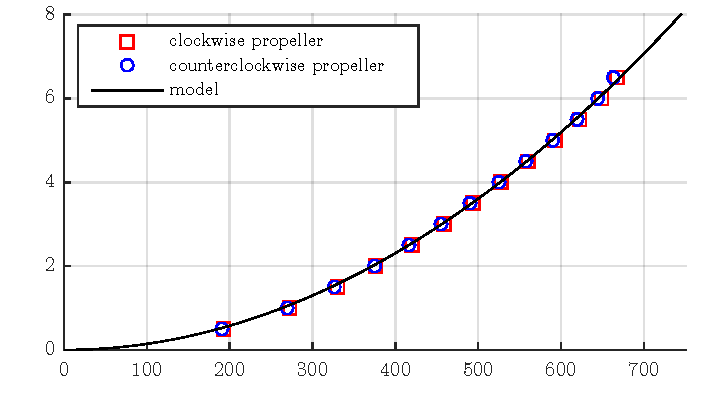
\includegraphics[scale=0.7]{PropVel2Thrust}
%  \caption{Identification of the torque constant $\kappaF$}
%  \label{fig:PropVel2Thrust}
% \end{figure}
% 
% \paragraph*{Identification of the thrust dynamics.}
% For identification of the parameters $\kappaT$, $\BLDCTorqueConstant$ and $\BLDCFriction$ we apply a stair-like input signal for $\BLDCCurr$ (see \autoref{fig:PropIdentMeas}) to the BLDC driver.
% A Savitzky-Golay-filter is applied to the measured propeller velocity $\PropVel$ which also yields an approximation of its derivative $\PropVeld$.
% Finally, knowing the Propeller inertia $\PropInertia$ and the sampled measurements $\PropVel[k]$, $\PropVeld[k]$ and $\BLDCCurr[k]$, we can identify the parameters $\kappaT$, $\BLDCTorqueConstant$ and $\BLDCFriction$ by the method of least squares.
% Overall the propeller drive model parameters are
% \begin{align}
%  \PropInertia &= 2.83 \cdot 10^{-5}\,\tfrac{\unit{N}\,\unit{m}\,\unit{s}^2}{\unit{RAD}},&
%  \kappaF &= 1.44 \cdot 10^{-5} \, \tfrac{\unit{N}\, \unit{s}^2}{\unit{RAD}^2},&
%  \kappaT &= 1.84 \cdot 10^{-7} \, \tfrac{\unit{N}\, \unit{m}\, \unit{s}^2}{\unit{RAD}^2},
% \nonumber\\
% &&
%  \BLDCTorqueConstant &= 1.39 \cdot 10^{-4} \unit{N}\, \unit{m},&
%  \BLDCFriction &= 4.97 \cdot 10^{-3} \unit{N}\, \unit{m}
%  .
% \end{align}
% The simulation result of the propeller model \eqref{eq:PropDriveModelVel} with the identified parameters is also shown in \autoref{fig:PropIdentMeas}.
% 
% Rather than the angular velocity $\PropVel$ we are actually interested in the thrust $\PropForce$ generated by the propeller.
% Elimination of the angular velocity $\PropVel$ from the model equations \eqref{eq:PropDriveModelVel} yields
% \begin{align}\label{eq:PropDriveModelForce}
%  \PropForceTimeConstant(\PropForce\,) \PropForced + \PropForce &= \PropForceInput(\BLDCCurr),
% \end{align}
% where
% \begin{align}
%  \PropForceTimeConstant(\PropForce\,) = \tfrac{\PropInertia \sqrt{\kappaF} }{2\kappaT \sqrt{\PropForce}} = \tfrac{\PropInertia}{2\kappaT \PropVel},
% \quad
%  \PropForceInput(\BLDCCurr) = \tfrac{\kappaF \BLDCTorqueConstant}{\kappaT} \BLDCCurr - \tfrac{\kappaF \BLDCFriction}{\kappaT}
%  .
% \end{align}
% The input characteristic $\PropForceInput(\BLDCCurr)$ is the stationary thrust for a constant input $\BLDCCurr$ and the time characteristic $\PropForceTimeConstant(\PropForce\,)$ corresponds to the time constant for a linear approximation about the working point $\PropForce$. 
% In \autoref{fig:PropIdentRes} the identified characteristics $\PropForceInput(\BLDCCurr)$ and $\PropForceTimeConstant(\PropForce\,)$ are compared to the measurements.
% 
% \paragraph*{Saturation.}
% One can see the beginning of a saturation for the stationary thrust $\PropForceInput$ which becomes stronger for a lower supply voltage (battery) to the power electronics.
% However, since this effect is far away from usual working conditions ($\PropForce \approx 2.5\,\unit{N}$ for quadcopter and $\PropForce \approx 4\,\unit{N}$ for tricopter hover) it is not considered in the model.
% Consequently the least squares identification of the model parameters is also only performed on measurement data for which $\BLDCCurr \leq 600$ to have a good model in the typical working regime.
% 
% \begin{figure}[p]
%  \centering
%  \includegraphics[scale=0.7]{PropIdentMeas.pdf}
%  \caption{Measurements for identification and simulation result}
%  \label{fig:PropIdentMeas}
% \vspace{15mm}
%  \includegraphics[scale=0.7]{PropIdentRes.pdf}
%  \caption{Identified input $\PropForceInput(\BLDCCurr)$ and time characteristic $\PropForceTimeConstant(\PropForce\,)$ of the propeller drive}
%  \label{fig:PropIdentRes}
% \end{figure}
% 
% \paragraph*{Observer.}
% The velocity measurement $\PropVelMeas[]$ is noisy, so it should not be used directly for feedback control.
% On the other hand, Low-pass filtering would lead to undesired delay.
% A solution is the use of an observer which can be regarded as a low-pass filter with a feed forward term that eliminates the delay.
% The implementation is a copy of the forward Euler discretization of the nonlinear model \eqref{eq:PropDriveModelVel} supplemented by a linear feedback of the error to the measurement
% \begin{multline}\label{eq:PropObserver}
%  \PropForceObs[][k] = \kappaF (\PropVelObs[][k])^2, \qquad
%  \tfrac{\PropInertia}{\Ts} (\PropVelObs[][k+1] - \PropVelObs[][k]) + \kappaT (\PropVelObs[][k])^2 = \BLDCTorqueConstant \BLDCCurr[][k] - \BLDCFriction
% \\
%  + l_{\PropVel} \big( \PropVelMeas[][k] - \tfrac{1}{2}(\PropVelObs[][k] + \PropVelObs[][k-1]) \big)
%  .
% \end{multline}
% Note that this leads to second order dynamics for the observer error due to the delay of the measurement.
% However, for reasonable values of the observer gain $l_{\PropVel}$ there is a very fast ``eigenvalue`` that can be neglected and a slower one that can be tuned with the observer gain.
% % closed loop
% % \begin{align}
% %  \PropVelObsErr[][k+1] + \big( \tfrac{2\Ts\kappaT \PropVel[]}{\PropInertia} + \tfrac{\Ts l_{\PropVel}}{2\PropInertia} - 1 \big) \PropVelObsErr[][k] + \tfrac{\Ts l_{\PropVel}}{2\PropInertia} \PropVelObsErr[][k-1] &= \tfrac{\Ts l_{\PropVel}}{\PropInertia} n[k]
% % \end{align}
% 
% \paragraph*{Prefilter.}
% The higher level controllers compute the desired thrust $\PropForceD[][k+1]$ for the next sampling step.
% Since the propeller thrust $\PropForce[]$ has a dynamic of its own \eqref{eq:PropDriveModelForce}, it is not possible to track this signal exactly (without additional information).
% 
% \fixme{
% We consider a combination of a prefilter and a feedback of the error \wrt to the filtered reference $\PropForceDFilt$.
% This approach is sometimes called \fixme{\textit{two degrees of freedom controller}} (\eg \cite{Zeitz:FlatnessSISO}) since it allows independent tuning of the tracking behavior and the closed loop stability.
% }
% 
% The implemented prefilter is the exact discretization of a low-pass filter with the time constant $\TPropForceFilter > \Ts$
% \begin{align}\label{eq:PropPrefilter}
%  \PropForceDFilt[][k+2] = \cPropForceFilter \PropForceDFilt[][k+1] + (1-\cPropForceFilter) \PropForceD[][k+1],
% \qquad
%  \cPropForceFilter = \exp (-\tfrac{\Ts}{\TPropForceFilter})
%  .
% \end{align}
% Note that for the filtered desired thrust $\PropForceDFilt[][k+1]$, we also have the value for the next sampling step $\PropForceDFilt[][k+2]$.
% 
% \paragraph*{Tracking controller.}
% For the tracking error $\PropForceE[]$ we set the desired response as
% \begin{align}\label{eq:ProperrorDyn}
%  \PropForceE[][k+1] = \PropCtrlParam[][k] \, \PropForceE[][k],
% \qquad
%  \PropForceE[][k] = \PropForceDFilt[][k] - \PropForceObs[][k]
%  .
% \end{align}
% Combination with the (forward Euler) discretization of the model \eqref{eq:PropDriveModelForce} yields the corresponding control law
% \begin{multline}\label{eq:PropController}
%  \BLDCCurr[][k+1]
%  = \underbrace{\tfrac{\kappaT}{\kappaF\BLDCTorqueConstant}\big( \tfrac{\PropInertia}{2 \kappaT \Ts \PropVelObs[][k+1]} \big(\PropForceDFilt[][k+2] - \PropForceDFilt[][k+1]\big) + \PropForceDFilt[][k+1] \big) + \tfrac{\BLDCFriction}{\BLDCTorqueConstant}}_{\text{feed-forward}}
% \\[-1.5ex]
%  + \overbrace{\underbrace{\tfrac{\kappaT}{\kappaF\BLDCTorqueConstant}\big( \tfrac{\PropInertia (1 - \PropCtrlParam[][k+1])}{2 \kappaT \Ts \PropVelObs[][k+1]} - 1 \big)}_{K_\textsf{FC}[k+1]}\PropForceE[][k+1]}^{\text{feedback}}
% \end{multline}
% 
% The closed loop parameter $\PropCtrlParam[][k]$ introduced in \eqref{eq:ProperrorDyn} is chosen as an affine function of the current (observed) angular velocity
% \begin{align}\label{eq:PropCtrlParam}
%  \PropCtrlParam[][k] = \PropCtrlParam[0] + \PropCtrlParam[1] \PropVelObs[][k]
%  .
% \end{align}
% Choosing $\PropCtrlParam[1]=0$ would lead to linear error dynamics, but would result in a high feedback gain $K_\textsf{FC}$ at low velocity $\PropVel$.
% On the other hand choosing $\PropCtrlParam[0]=1$ would lead to a constant feedback gain $K_\textsf{FC}$ which is too strong at high and too weak at low velocities.
% With \eqref{eq:PropCtrlParam} one can find a practical balance between these extreme cases.
% 
% \paragraph*{Tuning and validation.}
% The following parameters are used for the propeller control
% \begin{align}
%  l_{\PropVel} &= 7 \cdot 10^{-4}\, \tfrac{\unit{kg}\,\unit{m}^2}{\unit{s}},&
%  \TPropForceFilter &= 4 \Ts = 0.02\,\unit{s},&
%  \PropCtrlParam[0] &= 0.95,&
%  \PropCtrlParam[1] &= -8.40 \cdot 10^{-5} \unit{s}
%  .
% \end{align}
%  \autoref{fig:PropCtrlRes}.
% 
% \begin{figure}[h!]
%  \centering
%  \includegraphics[scale=0.7]{PropTimeCharacteristics.pdf}
%  \caption{Time characteristic of the propeller thrust control}
%  \label{fig:PropTimeCharacteristics}
% \end{figure}
% 
% 
% 
% \subsection{Servo model}
% The tiling mechanisms of the Tricopter are driven by hobbyist servo motors.
% Each is interfaced by a pulse width modulated signal corresponding to the desired angle $\aServoR$.
% 
% We consider the second order model whose parameters have been identified with a dedicated experiment
% \begin{align}
%  \aServodd + 2\zetaServo \wServo \aServod + \wServo^2 \aServo = \wServo^2 \aServoR,
% \qquad
%   \wServo = 39\,\unit{s}^{-1}, \ \zetaServo = 0.93
% \end{align}
% 
% Discrete simulator for the servo angle using the forward Euler approximation
% \begin{subequations}
% \begin{align}
%  \aServoObs[][k+1] &= \aServoObs[][k] + \Ts \aServoObsd[][k]
% \\
%  \aServoObsd[][k+1] &= \aServoObsd[][k] + \Ts( \wServo^2 (\aServoR[][k] - \aServoObs[][k]) - 2\zetaServo \wServo \aServoObsd[][k])
%  .
% \end{align}
% \end{subequations}
% 
% See \autoref{fig:ServoObsRes}.
% 
% \begin{figure}[p]
%  \centering
%  \includegraphics[scale=0.65]{PropCtrlRes/PropCtrlRes.pdf}
% % \vspace{-2mm}
%  \caption{Thrust control result}
%  \label{fig:PropCtrlRes}
% \vspace{3ex}
%  \includegraphics[scale=0.65]{ServoSimRes/ServoSimRes.pdf}
% % \vspace{-2mm}
%  \caption{Comparison of measured and simulated servo angle}
%  \label{fig:ServoObsRes}
% \end{figure}
\section{State estimation}\label{sec:RealizationStateEstimation}
The rigod body controller requires the current rigid body state (position, velocity, attiude and angular velocity) and the assumed offset force and torque.
The subject of this section is the estimation of these values based on the available measurements from IMU and motion capturing system.

\paragraph{Rigid body dynamics.}
The rigid body attitude may be parameterized by a unit quaternion $\quat = [\quatw, \quatx, \quaty, \quatz] \in \Sphere^3$ which allows for a more efficient implementation of the microcontroller and is pretty common in this field.
The corresponding kinematics may be derived as proposed in \autoref{sec:MathCoordinates}.
Furthermore, using the velocity coefficients $\rd$ w.r.t. the reference frame, the rigid body dynamics are
\begin{subequations}\label{eq:RealizationStateDyn}
\begin{align}
 m (\rdd - \gravityAcc) + d \rd = \RotMatQuat(\quat) (\F + \FB)
\\
 \quatd = \kinMatQuat(\quat) \, \w, \qquad
 \bodyMOI{}{} \dot{\w} + \wedOp(\w) \bodyMOI{}{} \w = \bodyTorque{}{} + \tauB
\end{align}
with
\begin{align}
 \RotMatQuat(\quat) &=
 \begin{bmatrix} 
  1 - 2(\quaty^{2} + \quatz^{2}) & 2(\quaty\quatx -\quatw\quatz)  & 2(\quatz\quatx + \quatw\quaty) \\
  2(\quaty\quatx + \quatw\quatz) & 1 - 2(\quatx^{2} + \quatz^{2}) & 2(\quaty\quatz - \quatw\quatx) \\
  2(\quatz\quatx - \quatw\quaty) & 2(\quaty\quatz + \quatw\quatx) & 1 - 2(\quatx^{2} + \quaty^{2})
 \end{bmatrix}
\\
 \kinMatQuat(\quat) &=
 \tfrac{1}{2} \begin{bmatrix}
  -\quatx & -\quaty & -\quatz \\
  \quatw & -\quatz &  \quaty \\
  \quatz &  \quatw & -\quatx \\
  -\quaty &  \quatx &  \quatw
 \end{bmatrix}
\end{align}
\end{subequations}

\paragraph{IMU measurements.}
The \textsc{VectorNav VN100s} contains a 3-axis accelerometer, gyroscope and magnetometer connected to microcontroller which implements an extended Kalman-filter to estimate the attitude quaternion and gyroscope biases.
While the attitude estimate is used for outdoor applications with the multicopter, it is not used here, as in the lab the more precise estimate from the motion capturing system available.
%Nevertheless, we will use the bias compensated gyroscope measurement.

Gyroscope and accelerometer measure the \textit{inertial} angular velocity and acceleration.
While for tactical and navigation grade IMUs the angular velocity of the Earth is an integral part of the navigation algorithms, see e.g.\ \cite{Savage:Strapdown1}, for the consumer grade IMU here, it cannot be distinguished from the reminescent bias in gyroscope.
Similarly, the coriolis acceleration on the accelerometer may be ignored and the only external parameter is Earth's gravity $\gravityAcc$ at the current position.

The IMU is mounted to the corresponding multicopter to roughly align with its body fixed frame, more precicly the body fixed frame determined by the reflective markers for the motion capture.
We will call the remaining, constant misalgnment $\RIMUBR \in \SpecialOrthogonalGroup(3)$.
While the gyroscope bias is compensated, the accelerometer contains a noticable slowly varying bias $\aIMUB \in \RealNum^3$.
Furthermore, both sensors contain a noticable noise $\wIMUN[k], \aIMUN[k] \in \RealNum^3$ which is not further investigated here.
Overall, with a constant sampling time $\Ts=0.005\,\unit{s}$, we assume the IMU measurments $\wIMU$ and $\aIMU$ to be related to the rigid body state by:
\begin{align}\label{eq:RealizationImuModel}
 \wIMU[k] &= \RIMUBR \w(k\Ts) + \wIMUN[k],
\\
 \aIMU[k] &=  \RIMUBR \R^\top(k\Ts) (\rdd(k\Ts) - \gravityAcc) + \aIMUB + \aIMUN[k]
 .
\end{align}

\paragraph{VICON measurements.}
The \textsc{VICON} motion capturing system measures the position $\r$ and the attitude, reported as quaternion $\quat$, by means of tracking the reflective markers on the multicopters.
The refernce frame of the system was carefully adjusted to align with gravity using a pendulum with reflective markers.

In contrast to the IMU measurments, there is no evidence for systematic errors in the measurements for the VICON system.
However, their processing and transmission to to the multicopter processor results in a substantial latency, i.e.\ measurements corresponding to time $t$ are available to the controller only after time $t+\TVICD$.
Furthermore, as non-realtime systems are involved, the latency varies slightly.
Mostly due to bandwidth limitations on the wireless transmission, the sampling time is only $\TsVIC=0.1\,\unit{s}$ while the main controller runs at $\Ts=0.005\,\unit{s}$.
The measurements $\rVIC$ and $\qVIC$ are related to the rigid body state by
\begin{align}
 \rVIC[k'] = \r(k'\TsVIC - \TVICD),
\qquad
 \qVIC[k'] = \quat(k'\TsVIC - \TVICD).
\end{align}

\begin{figure}
 \centering
 \input{graphics/StateEstimationBlock.pdf_tex}
 \caption{Overall structure of the state estimation}
 \label{fig:StateEstimationBlock}
\end{figure}

\paragraph{Overall observer design.}
Instead of designing one large observer, the estimation problem is split into smaller subproblems as illustrated in \autoref{fig:StateEstimationBlock}.
The the following subsections will discuss these.




\subsection{IMU misalignment correction}
For a static $\sysCoord=\const$ multicopter the accelerometer model reads
\begin{align}
 \aIMU[k] &=  -\RIMUBR \R^\top \gravityAcc + \aIMUB + \aIMUN[k].
\end{align} 
Here we are interested in the value $\RIMUBR$, but for its estimation propsed here we also need to estimate the accelerometer bias $\aIMUN$.
For a shorttime measurment ($\Delta t<10\,\unit{min}$) is can be assumed to be constant.
Taking into account that the reference frame was carefully aligned, and the official gravitation value for Saarland, we have $\gravityAcc = [0, 0, -9.8107]^\top \tfrac{\unit{m}}{\unit{s}^2}$.

The multicopter is placed in different random orientations while the accelerometer measurements $\aIMU$ and the attitude $\R$ is recorded.
To compensate the noise $\aIMUN[k]$ we take the mean value $\bar{\tuple{a}}_{\idxText{M}}$ over $10\,\unit{s}$.
For each measurement with index $i$ and different attitudes $\bar{\R}[i]$ we have the mean accelerometer measurement $\bar{\tuple{a}}_{\idxText{M}}[i]$.
With this, we estimate the values for misalignment $\RIMUBR$ and bias $\aIMUB$ as the ones that minimize the sum over the squared errors of the experiments:
\begin{align}
 \mathcal{J}(\RIMUBR, \aIMUB) = \tfrac{1}{2} \sum_i \norm{ \bar{\tuple{a}}_{\idxText{M}}[i] + \RIMUBR \bar{\R}^\top[i] \gravityAcc + \aIMUB }^2
\end{align}
Note that this minimization problem is mathematically identical to the one considered in \autoref{sec:RBStiffness}.

\begin{figure}[htb]
 \centering
 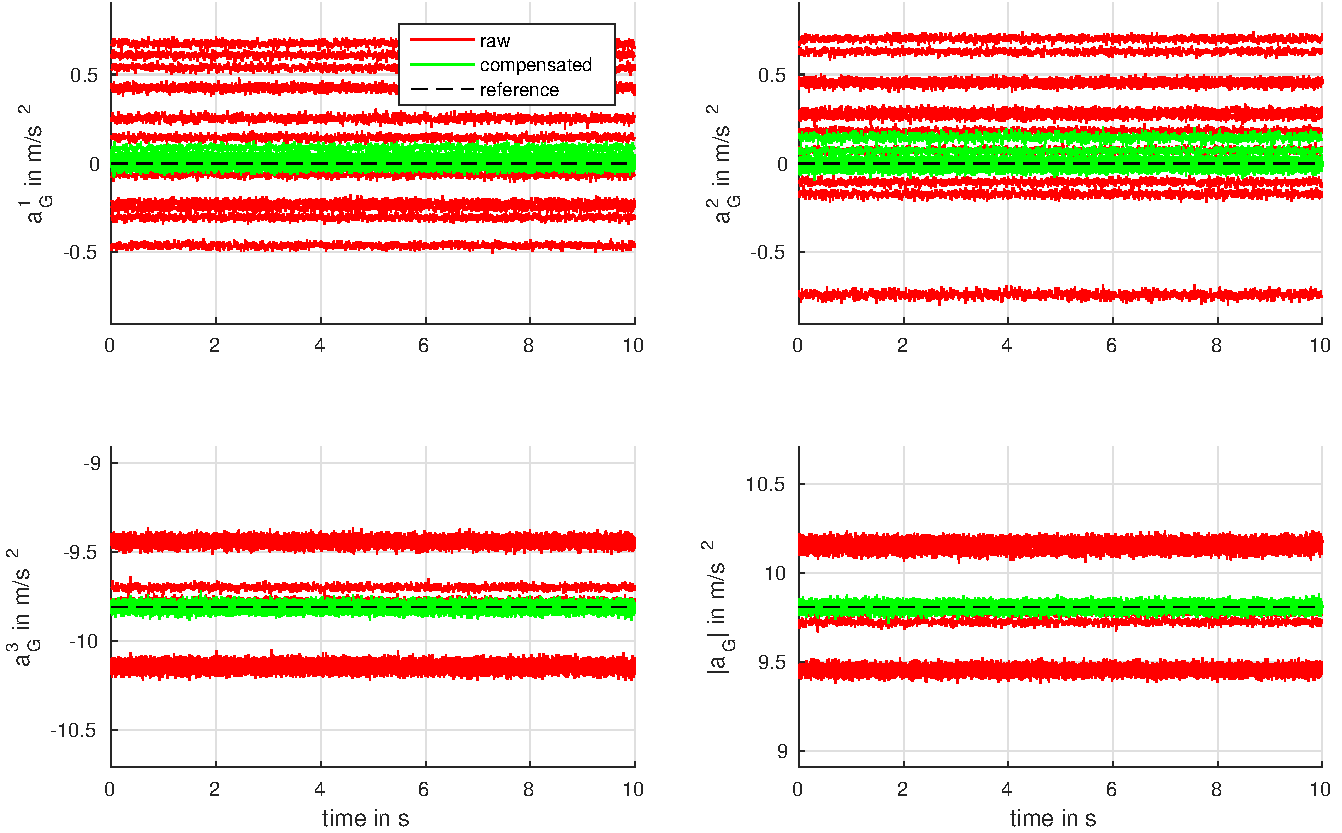
\includegraphics[scale=0.7]{AccBias.pdf}
 \caption{Accelerometer measurements and identification result}
 \label{fig:AccBias}
\end{figure}

For validation \autoref{fig:AccBias} displays the measured gravity coefficients $\gravityAcc$ within the 20 experiments with different orientations.
The red lines are the raw measurements $\gravityAcc = \RVIC \aIMU$, the green lines incorporate the identified values $\gravityAcc = \RVIC \RIMUBR (\aIMU + \aIMUB)$ and the black line is the reference value $\gravityAcc = [0,0,-9.81]^\top$.
Most notably one can see that even the magnitude $\norm{\gravityAcc}$ of the raw acceleration is off by about $5\%$ for some experiments whereas the compensated values are all within a window of about $0.2\%$.

\subsection{Angular velocity and torque bias}
Recall the mechanical model of the angular velocity $\w$, disturbance torque $\tauB$ and gyroscope $\wIMU$ motivated above:
\begin{align}
 \J \dot{\w} + \wedOp(\w) \J \w = \bodyTorque{}{} + \tauB,
\qquad
 \dot{\tau}_{\textsf{B}} = \tuple{0},
\qquad
 \wIMU = \w + \wIMUN.
\end{align}
The input torque $\bodyTorque{}{}$ is known as discussed in \autoref{sec:RealizationForceVectorControl}.

The multicopters implement a simple Luenberger observer based on the forward Euler discretization and scalar gains $L_\omega, L_\tau$: 
\begin{subequations}\label{eq:AngVelObs}
\begin{align}
 \wObs[\kPlusOne] &= \wObs[k] + \Ts \J^{-1} \big( \bodyTorque{}{}[k] + \tauBObs[k] - \wedOp(\wObs[k]) \J \wObs[k] \big) + L_\omega (\wIMU[k] - \wObs[k])
\\
 \tauBObs[\kPlusOne] &= \tauBObs[k] + L_\tau (\wIMU[k] - \wObs[k])
 .
\end{align}
\end{subequations}
In practice, the gains $L_\omega = 0.2$ and $L_\tau=0.01$ did yield good results.
The disturbance observer here takes the place of the integral controller, as the rigid body controller is "just" a PD controller.

% side calculation
% \begin{align}
%  -\wedOp(\w[k]) \Theta \w[k] + \wedOp(\wObs[k]) \Theta \wObs[k]
%  &= -\wedOp(\w[k]) \Theta \w[k] + \wedOp(\w[k] - e_\w[k]) \Theta (\w[k] - e_\w[k])
% \\
%  &= \wedOp(e_\w[k]) \Theta e_\w[k] - \wedOp(\w[k]) \Theta e_\w[k] - \wedOp(e_\w[k]) \Theta \w[k]
% \\
%  &= \wedOp(e_\w[k]) \Theta e_\w[k] + \big(\wedOp(\Theta \w[k]) - \wedOp(\w[k]) \Theta \big) e_\w[k]
% \end{align}
% \begin{align}
%  e_\w[\kPlusOne] &= e_\w[k] + \Ts e_\tau[k] - L_{\w} e_\w[k] - L_{\w} \wIMUN
% \nonumber\\
%  &\qquad \Ts \big( \wedOp(e_\w[k]) \Theta e_\w[k] + \big(\wedOp(\Theta \w[k]) - \wedOp(\w[k]) \Theta \big) e_\w[k] \big)
% \\
%  e_\tau[\kPlusOne] &= e_\tau[k] - L_\tau e_\w[k] - L_\tau \wIMUN
% \end{align}
% Introducing the error quantities $e_{\w} = \w - \wObs$ and $e_\tau = \tauB - \tauBObs$ and subtracting the observer \eqref{eq:AngVelObs} from the discretized model we find the \textit{observer error dynamics}:
% \begin{multline}\label{eq:AngVelObsErrorDyn}
%  \begin{bmatrix} e_{\w}[\kPlusOne] \\ e_{\tau}[\kPlusOne] \end{bmatrix} 
%  = \begin{bmatrix} 
%   \idMat[3] - L_{\w} - S(\w[k]) & \Ts \J^{-1} \\
%   - L_{\tau} & \idMat[3]
%  \end{bmatrix}
%  \begin{bmatrix} e_{\w}[k] \\ e_{\tau}[k] \end{bmatrix}
% \\
%  +
%  \begin{bmatrix} \Ts \J^{-1} \wedOp(e_{\w}[k]) \Theta e_{\w}[k] \\ 0 \end{bmatrix} 
%  -
%  \begin{bmatrix} L_{\w} \\ L_{\tau} \end{bmatrix} 
%  \wIMUN
% \end{multline}
% where
% \begin{align}
%  S(\w[k]) = \Ts \J^{-1} \big( \wedOp(\w[k]) \Theta - \wedOp(\Theta \w[k]) \big).
% \end{align}
% Note that the term quadratic in $e_{\w}$ is negligible if assuming small errors.
% The term $S(\w[k])$ contains the time-variant part of the error dynamics.
% However, for a reasonable gain $L_{\w}$ and typical working conditions (\eg $\norm{\w} < 10\,\sfrac{\unit{rad}}{\unit{s}}$) the gain $L_{\w}$ dominates over the time-variant part and the error dynamics are asymptotically stable.
% Furthermore, for the linearization about the hover case, $\w \approx 0$, the matrix $S$ drops out completely.
% This is used to compute the gains $L_{\w} = \diag(l_{\wx}, l_{\wy}, l_{\wz})$ and $L_{\tau} = \diag(l_{\taux}, l_{\tauy}, l_{\tauz})$ corresponding to given desired closed loop poles at this expansion point.


\subsection{Configuration measurement latency}
The configuration measurement $(\rVIC, \qVIC)$ is done by a \textsc{Vicon} motion capturing system.
This measurement relies on the optical tracking of reflective markers fixed on the multicopters by infrared cameras mounted at the walls of the lab and connected to the ground station, a Windows 7 PC.
The groundstation software is written in \textsc{Matlab}.
It runs a timer at $\TsVIC = 0.1\,\unit{ms}$ which reads the measurement, validates and forwards it to the xBee radio module.
Finally, the multicopter microcontroller receives the measurements through its ratio module.
The radio module also handles other transmitions like receiving commands and sending measurements to the groundstation.

As a result of this chain of non realtime elements, the latency at which the configuration measurements are available to the multicopter is \textit{not} constant, but varies by several main sampling steps $\Ts$ in addition to its average value.
Actual timings of these measuremnts are presented in \autoref{fig:ViconDelayIllustrate} for actual measurements.
The estimation of the resulting \textit{variable time delay} $\TVICD[k']$ is the subject of this subsection.

\begin{figure}[htb]
 \centering
 \input{graphics/ViconDelayClocks.pdf_tex}
 \caption{Illustration of the measurement time at the PC and when it is available on the microcontroller (MC)}
 \label{fig:ViconDelayClocks}
\end{figure}

To get an estimate $\TVICDObs[k']$ for this delay we utilize the clocks on the ground station PC, $t'$, and the microcontroller, $t$.
The clocks are assumed to be synchronous but have an unknown offset $\TPC = t - t' = \const$ depending on when each device was powered.
\autoref{fig:ViconDelayClocks} illustrates the time $\tVICp[k']$ at which a measurement was taken and the time $\tRec[k']$ at which it is received/available on the microcontroller.
Taking a large enough sample of these times we have the relation
\begin{align}\label{eq:meanTPC}
 \text{mean} (\tRec[1,\ldots,K'] - \tVICp[1,\ldots,K']) = \TPC + \text{mean}(\TVICD[1,\ldots,K']), \quad K'\gg 1.
\end{align}
Whereas $\TPC$ changes whenever the ground station or the micocontroller restarts, the average delay $\meanTVICD = \text{mean}(\TVICD[1,\ldots,K'])$ remains constant.

\paragraph{Experimental average delay identification.}
The identification of the average delay $\meanTVICD$ is done in a dedicated experiment:
A multicopter is mounted on an incremental encoder directly connected to the multicopter main processor.
It serves as a reference for the yaw-angle and is assumed to have negligible latency.
The encoder signal and the yaw-angle from the motion capture system are recorded by the multicopter microcontroller.
The experimental data here is about $1\,\unit{min}$ long and captures about $K' = 600$ \textsc{Vicon} frames.
Now we can plot the reference encoder angle $\yaw[k]$ at the sampling points $t = k\Ts$ and the yaw angle $\yawVIC[k']$ received from the Vicon system at the shifted time $\tVICp[k'] + \text{mean}(\tRec[1,\ldots,K'] - \tVICp[1,\ldots,K'])$.
If the previous assumption \eqref{eq:meanTPC} hold theses signals should be similar up to a shift of the mean delay $\meanTVICD$.

\begin{figure}[ht]
 \centering
 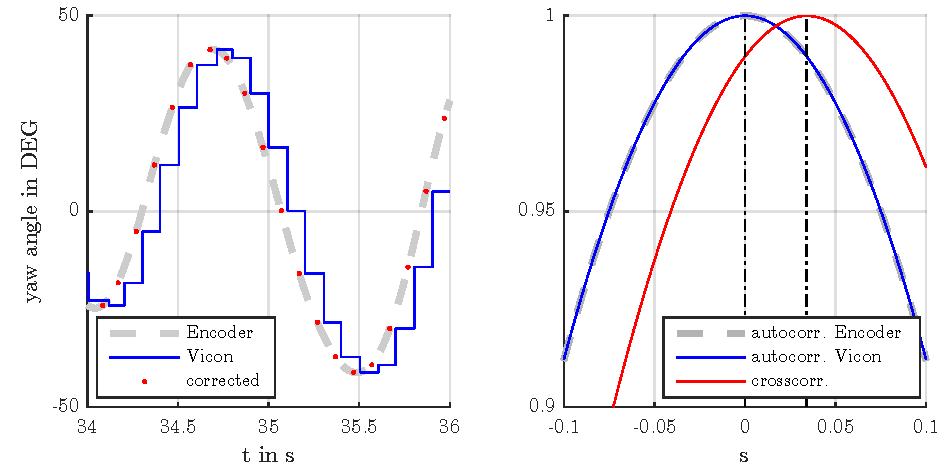
\includegraphics{ViconDelay/ViconDelayIdent.pdf}
 \caption{A small sample of the yaw-angle measurements (left) and the correlations (right) of the complete $60\,\unit{s}$ measurements for the identification of the average time delay}
 \label{fig:ViconDelayIdent}
\end{figure}

\autoref{fig:ViconDelayIdent} shows a small sample of the measured yaw angle and the correlations of the two measurements.
The identified average delay is where the cross-correlation has its maximum at $\meanTVICD = 0.034\,\unit{s}$.
In order to achieve this resolution the measurements were up-sampled to $1\,\unit{ms}$ by cubic interpolation.


\paragraph{Clock offset estimation.}
For the realtime implementation, \eqref{eq:meanTPC} is approximated by a slow ($\cTPC = 0.99$) low-pass filter
\begin{align}
 \TPCObs[k'] = \cTPC \TPCObs[k'\!-\!1] + (1-\cTPC) (\tRec[k'] - \tVICp[k'] - \meanTVICD)
\end{align}
yielding the estimate $\TPCObs$ for the constant clock offset $\TPC$.
Finally, the estimated delay of the $k'$-th Vicon measurement is
\begin{align}
 \TVICDObs[k'] = \tRec[k'] - \big( \tVICp[k'] + \TPCObs[k'] \big).
\end{align}
\autoref{fig:ViconDelayIllustrate} shows the estimated clock offset $\TPCObs$ and the resulting estimated delay $\TVICDObs$ for the previous example measurement.

\begin{figure}[ht]
 \centering
 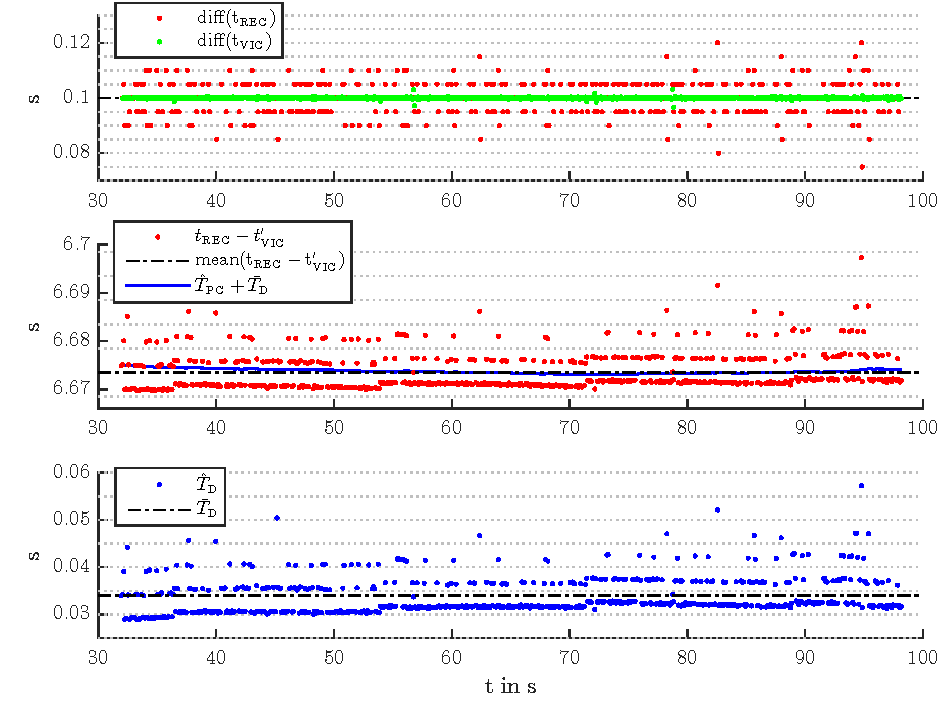
\includegraphics{graphics/ViconDelay/ViconDelayIllustrate}                                                                    
 \caption{Measured timings}
 \label{fig:ViconDelayIllustrate}
\end{figure}

\subsection{Attitude integration}
Once the latency $\TVICDObs[k']$ of the attitude measurement $\qVIC$ is known, the current attitude is simply integrated based on buffered angular velocity measurements.
The quaternion kinematics \eqref{eq:RealizationStateDyn} supplemented with a stabilization term for the constraint $\quat \in \Sphere^3$, as motivated in \autoref{sec:ConstraintStabilization}, reads
\begin{align}\label{eq:QuaternionKinematics}
 \tdiff{t} \underbrace{\begin{bmatrix} \quatw \\ \quatx \\ \quaty \\ \quatz \end{bmatrix}}_{\quat}
 = \underbrace{\tfrac{1}{2} \begin{bmatrix} -\quatx & -\quaty & -\quatz \\ \quatw & -\quatz & \quaty \\ \quatz & \quatw & -\quatx \\ -\quaty & \quatx & \quatw \end{bmatrix}}_{\kinMatQuat(\quat)}
 \underbrace{\begin{bmatrix} \wx \\ \wy \\ \wz \end{bmatrix}}_{\w}
 -
 \underbrace{\tfrac{1}{2} \begin{bmatrix} \quatw \\ \quatx \\ \quaty \\ \quatz \end{bmatrix}}_{\left(\pdiff[\geoConstraint]{\quat}(\quat)\right)^+}
 \lambda\underbrace{(\norm{\quat}^2 - 1)}_{\geoConstraint(\quat)}
 .
\end{align}
The actual implementation uses the forward Euler discretization with the stabilization gain $\lambda=\sfrac{2}{\Ts}$, i.e.\
\begin{align}\label{eq:QuaternionKinematicsDiscrete}
 \quat[k\!+\!1] = \quat[k] + \Ts \kinMatQuat(\quat[k]) \w[k] - (\norm{\quat[k]}^2-1) \quat[k].
\end{align}
Note that with this particular gain the stabilization coincides with the 1st order Taylor expansion of the normalization $\sfrac{\quat}{\norm{\quat}} \approx \quat - (\norm{\quat}^2-1) \quat$ for $\norm{\quat} \approx 1$.
In contrast to the exact normalization, the approximation avoids the expensive computation of a square root and division.

% \paragraph{Attitude integration.}
% From the previous subsection we know the micro controller time $\tVIC[k'] = \tRec[k'] - \TVICDObs[k']$ at which the received attitude measurement $\qVIC[k']$ was taken.
% To get the an estimate $\quatObs[k]$ for the current attitude we \textit{integrate} the attitude quaternion kinematics \eqref{eq:QuaternionKinematicsDiscrete} using the measurement $\qVIC[k']$ as initial value and the (ring) buffered angular velocity estimates $\wObs[k-\text{floor}(\sfrac{\TVICDObs[k']}{\Ts})],\ldots, \wObs[k]$.
% Since the delay $\TVICDObs[k']$ is usually not a multiple of the micro controller sampling time $\Ts$ a linear interpolation of the angular velocity $\wObs(\tVIC[k'])$ is used.


\subsection{Position, velocity and accelerometer bias}
For the translational dynamics we have a similar situation as for the attitude kinematics:
We have a acurate but low sampled and delayed position measurement $\rVIC$ and a biased and noisy measurement of the acceleration $\aIMU$.
From this we want to estimate the current position $\r$ and velocity $\rd$ required for the controller implementation.

The differential relation between position and accelerometer measurement is givein in \eqref{eq:RealizationImuModel}. 
For the following we assume a constant bias $\aIMUBd = \tuple{0}$ and drop the noise term $\aIMUN = \tuple{0}$.
Furthermore, the IMU misalignment has already been corrected, i.e.\ $\RIMUBR = \idMat[3]$.
Introducing the state $\tuple{z} = [\r^\top, \rd^\top, \aIMUB^\top]^\top \in \RealNum^9$ we may write 
%\begin{subequations}
\begin{align}\label{eq:AccelerometerDynamicsState}
 \tdiff{t}
 \underbrace{\begin{bmatrix} \r \\ \rd \\ \aIMUB \end{bmatrix}}_{\tuple{z}}
 &=
 \underbrace{\begin{bmatrix} 0 & \idMat[3] & 0 \\ 0 & 0 & -\R \\ 0 & 0 & 0 \end{bmatrix}}_{\mat{A}}
 \underbrace{\begin{bmatrix} \r \\ \rd \\ \aIMUB \end{bmatrix}}_{\tuple{z}}
 +
 \underbrace{\begin{bmatrix} 0 \\ \idMat[3] \\ 0 \end{bmatrix}}_{\mat{B}}
 \underbrace{(\gravityAcc + \R \aIMU)}_{\tuple{u}},&
 \rVIC &= \underbrace{[\idMat[3], \mat{0}, \mat{0}]}_{\mat{C}}
 \underbrace{\begin{bmatrix} \r \\ \rd \\ \aIMUB \end{bmatrix}}_{\tuple{z}}
\end{align}
%\end{subequations}

\paragraph{Estimator implementation.}
The implemented estimation algorithm on the \microcontroller works as follows:
After having received 2 subsequent position measurements $\rVIC[1]$, $\rVIC[2]$ and their reconstructed time $\tVIC[1]$, $\tVIC[2]$ with $\Ts'[1]=\tVIC[2]-\tVIC[1]$ we set the initial value for the estimator state $\hat{z} = [\rObs^\top, \rdObs^\top, \aIMUBObs^\top]^\top$ as
\begin{align}
 \rObs(\tVIC[2]) = \rVIC[2], 
\qquad
 \rdObs(\tVIC[2]) = \tfrac{\rVIC[2]-\rVIC[1]}{\Ts'[1]}
\qquad
 \aIMUB(\tVIC[2]) = \tuple{0}.
\end{align}
Then we use the zero order hold discretization of \eqref{eq:AccelerometerDynamicsState} to integrate the current state based on (ring) buffered accelerometer measurments $\aIMU$ and estimated attitudes $\RObs$:
\begin{align}\label{eq:PosPredictor}
 \underbrace{\begin{bmatrix} \rObs[\kPlusOne] \\ \rdObs[\kPlusOne] \\ \aIMUBObs[\kPlusOne] \end{bmatrix}}_{\hat{\tuple{z}}[\kPlusOne]}
 =
 \underbrace{\begin{bmatrix} \idMat[3] & \Ts\idMat[3] & -\tfrac{\Ts^2}{2}\RObs[k] \\ 0 & \idMat[3] & -\Ts\RObs[k] \\ 0 & 0 & \idMat[3] \end{bmatrix}}_{\hat{\mat{A}}_\idxSamp[k]}
 \underbrace{\begin{bmatrix} \rObs[k] \\ \rdObs[k] \\ \aIMUBObs[k] \end{bmatrix}}_{\hat{\tuple{z}}[k]}
 +
 \underbrace{\begin{bmatrix} \tfrac{\Ts^2}{2}\idMat[3] \\ \Ts \idMat[3] \\ 0 \end{bmatrix}}_{\mat{B}_\idxSamp}
 \underbrace{(\gravityAcc + \RObs[k] \aIMU[k])}_{\hat{\tuple{u}}[k]}
\end{align}
Note that the measurement time $\tVIC[2]$ usually does not coincide with a sampling step, see \autoref{fig:ViconDelayClocks}.
Consequently the value $\Ts$ in \eqref{eq:PosPredictor} has to be adjusted to match the time from the initial value to the subsequent sampling step.
%Furthermore the accelerometer measurement $\aIMU$ is linearly interpolated to approximate the acceleration at the initial time $\tVIC[2]$.
%The attitude $\R$ at the initial point is $\RotMatQuat(\qVIC[2])$ which is received simultaneously with $\rVIC[2]$.

After this initial procedure, \eqref{eq:PosPredictor} is computed once every sampling step with the most recent accelerometer measurement $\aIMU[k]$ yielding the most recent predictions for the position and velocity.
The position estimates $\rObs[k]$ for the last 64 sampling steps are stored in a ring buffer.

When a new configuration measurement $(\rVIC[k'], \RVIC[k'])$ and its timestamp $\tVIC[k']$ are available, the corresponding estimate $\rObs(\tVIC[k'])$ is interpolated.
This is used to correct the estimate \textit{at the measurement time} $\tVIC[k']$ with yet to define gains $\mat{L}_r, \mat{L}_v, \mat{L}_a \in \RealNum^{3\times3}$:
\begin{align}\label{eq:PosCorrector}
 \underbrace{\begin{bmatrix} \rObs(\tVIC[k']) \\ \rdObs(\tVIC[k']) \\ \aIMUBObs(\tVIC[k']) \end{bmatrix}}_{\hat{z}(\tVIC[k'])}
 \leftarrow 
 \underbrace{\begin{bmatrix} \rObs(\tVIC[k']) \\ \rdObs(\tVIC[k']) \\ \aIMUBObs(\tVIC[k']) \end{bmatrix}}_{\hat{z}(\tVIC[k'])}
 +
 \underbrace{\begin{bmatrix} \mat{L}_r[k'] \\ \mat{L}_v[k'] \\ \mat{L}_a[k'] (\RVIC[k'])^\top \end{bmatrix}}_{\mat{L}[k']}
 (\rVIC[k'] - \rObs(\tVIC[k'])).
\end{align}
Finally, the state estimate \textit{for current time} is again integrated from \eqref{eq:PosPredictor}.


\paragraph{Error dynamics and tuning.}
To chose reasonable correction gains $\mat{L}_r$, $\mat{L}_v$ and $\mat{L}_a$ we investigate the resulting error dynamics of the estimation algorithm above.
Assuming the attitude is constant and perfectly known $\RObs = \bar{\R}$ the matrix $A$ in the continuous model \eqref{eq:AccelerometerDynamicsState} is constant and is denoted by $\bar{\mat{A}}$.

From measurement time $\tVIC[k']$ till the next one at $\tVIC[k'+1]$ there are several prediction steps \eqref{eq:PosPredictor}:
The first from the measurement time till the subsequent sampling step with integration time $T_\mathsf{I}$.
Then several steps with integration time $\Ts$ till the sampling step before $\tVIC[k'+1]$, and finally a step integration time $T_\mathsf{F}$ till $\tVIC[k'+1]$.
Overall this results in the dynamic matrix 
\begin{align}
 \bar{\mat{A}}'_\idxSamp = \exp(\bar{\mat{A}}\,T_\mathsf{I}) \exp(\bar{\mat{A}}\,\Ts) \cdots \exp(\bar{\mat{A}}\,\Ts) \exp(\bar{\mat{A}}\,T_\mathsf{F}) = \exp(\bar{\mat{A}}\,\Tsp), 
\end{align}
where $\Tsp[k'] = T_\mathsf{I}[k'] + \Ts + \ldots + \Ts + T_\mathsf{F}[k'] = \tVIC[k'] - \tVIC[k'-1]$.
%Since $\Tsp[k']$ is known and exploiting this property of the exponential map, we do not need to worry about the different integration times of the predictions.

Finally, adding one correction step \eqref{eq:PosCorrector} and subtracting the estimator from the discretization of the model \eqref{eq:AccelerometerDynamicsState}, we obtain the relation for the error $\tuple{e} = \tuple{z} - \hat{\tuple{z}}$ for one correction/measurement cycle from $\tVIC[k']$ to the next one at $\tVIC[k'+1]$ as
\begin{align}
 \tuple{e}(\tVIC[k'\!+\!1]) = \underbrace{(\idMat[9] - \bar{\mat{L}}[k'] \mat{C}) \bar{\mat{A}}'_\idxSamp[k']}_{\bar{\mat{A}}'_e[k']} \tuple{e}(\tVIC[k'])
\end{align}
where
% \begin{align}
%  \bar{\mat{A}}'_\idxSamp[k'] &=
%  \begin{bmatrix}
%   \idMat[3] & \Tsp[k'] \idMat[3] & -\tfrac{(\Tsp[k'])^2}{2} \bar{\R} \\
%   0 & \idMat[3] & -\Tsp[k']\bar{\R} \\
%   0 & 0 & \idMat[3]
%  \end{bmatrix},&
%  \bar{\mat{L}}[k'] &= \begin{bmatrix} \mat{L}_r[k'] \\ \mat{L}_v[k'] \\ \mat{L}_a[k'] \bar{\R}^\top \end{bmatrix},&
%  \mat{C} &= [\idMat[3] \ 0 \ 0]
% \end{align}
% and finally
\begin{align}
 \bar{A}_e[k'] = 
 \begin{bmatrix} 
  \idMat[3] - \mat{L}_r[k'] & \Tsp(\idMat[3] - \mat{L}_r[k']) & \tfrac{(\Tsp[k'])^2}{2}(\mat{L}_r[k'] - \idMat[3]) \bar{\R} \\
  -\mat{L}_v[k'] & \idMat[3] - \Tsp[k'] \mat{L}_v[k'] & \Ts(\tfrac{\Tsp[k']}{2} \mat{L}_v[k'] - \idMat[3])\bar{\R} \\
  -\mat{L}_a[k'] \bar{\R}^\top & -\Tsp[k'] \mat{L}_a[k'] \bar{\R}^\top & \idMat[3] + \tfrac{\Tsp[k']^2}{2} \mat{L}_a[k']
 \end{bmatrix}
%  \begin{bmatrix} 
%   (1-l_r)\idMat[3] & \Ts'(1 - l_r)\idMat[3] & \tfrac{\Ts'^2}{2}(l_r - 1) \bar{\R} \\
%   -l_v \idMat[3] & (1-\Ts'l_v)\idMat[3] & \Ts(\tfrac{\Ts'}{2}l_v - 1) \bar{\R} \\
%   -l_a \bar{\R}^\top & -\Ts' l_a \bar{R}^\top & (1 + \tfrac{\Ts'^2}{2} l_a) \idMat[3]
%  \end{bmatrix}
\end{align}
Scaling the gains with the variable integration time $\Tsp[k']$ between two correction steps as
\begin{align}
 \mat{L}_r[k'] &= l_r \idMat[3],& 
 \mat{L}_v[k'] &= \tfrac{l_v}{\Tsp[k']} \idMat[3],&
 \mat{L}_a[k'] &= \tfrac{2 l_a}{(\Tsp[k'])^2}
\end{align}
yields the characteristic polynomial with constant coefficients
\begin{align}
 \det(\lambda \idMat[9] - \bar{A}'_e[k'])
 = \Big( \lambda^3
  + \big(l_r + l'_v - l'_a - 3 \big) \lambda^2
  + \big(3 - 2 l_r - l'_v - l'_a \big) \lambda
  + l_r - 1
 \Big)^3.
\end{align}
However, it should be noted here that constant eigenvalues of the time varying matrix $\bar{A}'_e[k']$ can not conclude stability of the time-varying system.

In practice the eigenvalues $\eig(\bar{A}'_e) = \{ 0, 0.5, 0.9 \}$ and the resulting gains $l_r = 1$, $l_v = 0.575$, $l_a = -0.025$ did result in quite good estimation performance.
These rather fast eigenvalues also reflect a high confidence in the position measurement.


\subsection{Force bias}
Combining the translational multicopter model \eqref{eq:RealizationStateDyn} and the accelerometer model \eqref{eq:RealizationImuModel}, we may write
\begin{align}
 \FB &= m (\aIMU - \aIMUN - \aIMUB) + d \RT \rd - \bodyForce{}{}.
\end{align}
From the previous sections we have estimates for the all quantities on the right hand side except the measurement noise $\aIMUN$.
This motivates a simple low-pass to obtain the estimate $\FBObs$ for the force bias
\begin{align}
 \FBObs[\kPlusOne] = l_F \FBObs[k] + (1 - l_F) \big( m (\aIMU[k] - \aIMUBObs[k]) + d (\RObs[k])^\top \rdObs[k] - \FObs[k] \big)
 .
\end{align}
In practice the low-pass gain $l_F = 0.98$ did yield reasonable results.
 
\section{Reference generation}
There are two ways for the user to interact with the \Multicopters: With a two joystick remote control (RC) or by sending various commands from the ground station PC.
The user inputs have to be transformed to yield corresponding reference values $(\rR, \RR, \vR, \wR, \vRd, \wRd)[k]$ for the \Multicopter controller.

The implemented procedure for doing so has two stages:
First the flatness of the \Multicopter models is exploited to reference values by a reference for the flat output with an intuitive interpretation.
If the RC is used, its joystick deflections have to be processed to yield the flat output components and their derivatives.
If the PC commands are used, they are processed to yield trajectories for the flat output.
%\ie $(y_\idxRef[k], \dot{y}_\idxRef[k], \ldots) \mapsto (\rR, \RR, \vR, \wR, \vRd, \wRd)[k]$.

\begin{itemize}
 \item Flatness
 \item Groundstation commands: Reference generation
 \item RC input: pilot supporting control
 \item Quadcopter integral action
\end{itemize}


\subsection{Flatness}\label{sec:RealizationRefGenFlatness}
For the discussion of flatness of the \Multicopter models we neglect the force and torque biases $\FB=0$ and $\tauB=0$.
Furthermore it is useful to express the models in terms of the translational velocity $\rd = \R \v$.

\paragraph{Tricopter.}
The \Tricopter model can be written as
\begin{subequations}\label{eq:RefGenTricopterModel}
\begin{align}
 \R^\top \R &= \idMat[3], \quad \det \R = +1,
\label{eq:RefGenTricopterGeoConstraint}
\\
 \Rd &= \R \wedOp(\w),
\\
 \J \dot{\w} + \wedOp(\w) \J \w &= \tau,
\\
 m(\rdd-\gravityAcc) + d \rd &= \R F.
\label{eq:RefGenTricopterTranslationalDyn}
\end{align}
\end{subequations}
Since the model is fully-actuated, any minimal parameterization of its configuration space is a flat output.
But since the configuration space is non-Euclidean, there is no global minimal parameterization.
In practice the \Tricopter cannot tilt too much anyway, so we will be content with a parameterization of the attitude $\R$ that is defined around the hover condition.

\paragraph{Quadcopter.}
For the \Quadcopter model we simply replace \eqref{eq:RefGenTricopterTranslationalDyn} by
\begin{align}
  m(\rdd-\gravityAcc) + d \rd = \R \ez \, \Fz.
\end{align}
The flatness of this model is extensively discussed in \cite{Konz:QuadrotorMovingFrame}.
From the number of inputs $\Fz \in \RealNum$ and $\tau \in \RealNum^3$ it is clear that a flat output has 4 components, i.e.\ $y \in \RealNum^4$.
We choose the position as the first 3 components $y_{1\ldots3} = r$ of the flat output.
From these we can already compute the total thrust $\Fz$ and the last column of the rotation matrix $\R$ as
\begin{align}\label{eq:RefGenQuadcopterConstraint}
 \Fz &= \pm \norm{m(\rdd-\gravityAcc) + d \rd},&
 \R \ez &= \sign(\Fz) \frac{m(\rdd-\gravityAcc) + d \rd}{\norm{m(\rdd-\gravityAcc) + d \rd}}.
\end{align}
Obviously this parameterization is singular for $\norm{m(\rdd-\gravityAcc) + d \rd} = 0$.
This singularity is intrinsic, i.e.\ it can not be avoided by a different parameterization.
A way to tackle this problem is discussed in \cite{Lenoir:2kPi}.

Here, due to practical limitations, we can only realize a strictly positive total thrust $0 < \FzMin \leq \Fz \leq \FzMax$ anyway.
So we don't need to worry about the singularity, if we ensure that the reference trajectory for the position obeys $\FzMin \leq \norm{m(\rdd-\gravityAcc) + d \rd} \leq \FzMax$.

The third column of the rotation matrix $\R$ is fixed by the first three components of the flat output $y_{1\ldots3} = r$ by \eqref{eq:RefGenQuadcopterConstraint}. 
So the remaining one degree of freedom of the rotation matrix has to be parameterized the remaining fourth component $y_4$ of the flat output.
This is a purely geometric problem:
Let $\Rx, \Ry, \Rz \in \RealNum^3$ be the columns of the rotation matrix, i.e.\ $\R = [\Rx,\Ry,\Rz]$.
The task is to find a continuous map $(y_4, \Rz) \mapsto (\Rx, \Ry)$ that obeys the geometric constraints \eqref{eq:RefGenTricopterGeoConstraint}.
Since the constraints imply $\Rz\times\Rx = \Ry$ we can eliminate $\Ry$ from the problem.
The reduced problem is to find a continuous map $(y_4, \Rz) \mapsto \Rx$ with the remaining constraints $\norm{\Rx} = 1$ and $\sProd{\Rz}{\Rx} = 0$.
Recall that $\Rz \in \RealNum^3$, $\norm{\Rz}=1$.
So geometrically the problem is finding a continuous unit vector field on the 2-sphere.
The \textit{hairy ball theorem} \cite{Brouwer:HairyBallTheorem} implies that any such vector field must have at least one singularity.
Even though unavoidable, this singularity is not intrinsic.
With a suitable parameterization of the rotation matrix $\R$ we can move it where it hurts least.

Any flat output $y_{1\ldots4}$ of the \Quadcopter supplemented with $y_5=\Fx$ and $y_6=\Fy$ is a flat output of the \Tricopter.

\paragraph{Rotation matrix decomposition.}
For $\varphi \in \RealNum$ and $\p = [\px,\py,\pz]^\top \in \Sphere^2 \backslash [0,0,-1]^\top$ we define the rotation matrices
\begin{align}
 \RotMatZ(\head) &=
 \begin{bmatrix}
  \cos\head & -\sin\head & 0 \\
  \sin\head & \cos\head & 0 \\
  0 & 0 & 1
 \end{bmatrix},&
 \RotMatPZ(\p) &=
 \begin{bmatrix}
  1 - \frac{(\px)^2}{1+\pz} & -\frac{\px \py}{1+\pz} & \px \\
  -\frac{\px \py}{1+\pz} & 1 - \frac{(\py)^2}{1+\pz} & \py \\
  -\px & -\py & \pz
 \end{bmatrix}.
\end{align}
The matrix $\RotMatZ$ is a rotation about the $\ez$ axis with angle $\head$ and $\RotMatPZ(\p)$ is a rotation about the axis $\ez \times p$ with the angle $\alpha = \cos^{-1} \pz$.
The matrix $\RotMatPZ$ can also be defined as the unique rotation matrix $\R$ that solves $\p = \R \ez$ and has the \textit{minimal angle} $\alpha = \cos^{-1} \tfrac{1}{2}(\tr \R - 1)$, see \cite{Konz:QuadrotorMovingFrame}.
In \autoref{fig:HairyBalls} the the three columns of $\RotMatPZ(\p)$ are illustrated as red, green and blue lines starting at the point $\p$ on the 2-sphere.
In particular it should illustrate the relation to the hairy ball theorem:
On the upper hemisphere the hair are combed quite well, whereas it gets more messy on the lower hemisphere with a cowlick at the southpole. 

% \begin{minipage}{\linewidth}
%  \centering
%  \input{graphics/IllustrateMinRotMat.pdf_tex}
%  \captionof{figure}{Illustration of $\RotMatZ(\head)$, left, and $\RotMatPZ(p)$, right}
%  \label{fig:IllustrateMinRotMat}
% \end{minipage}

%\begin{figure}[ht]
% 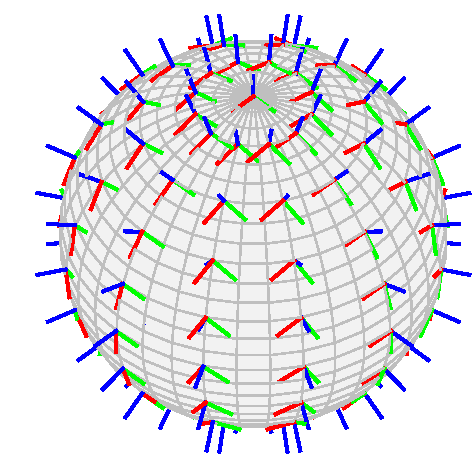
\includegraphics{HairyBall/HairyBallUpper.pdf}
% 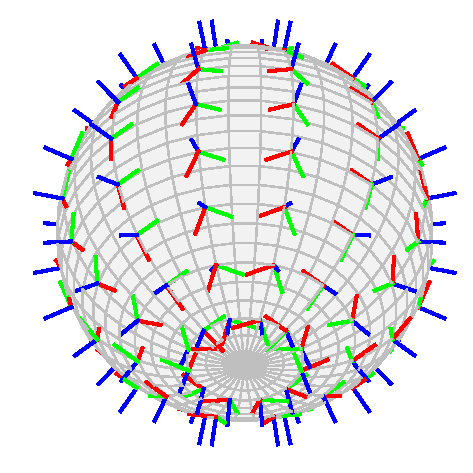
\includegraphics{HairyBall/HairyBallLower.pdf}
% \caption{Illustration of the rotation matrix $\RotMatPZ(\p)$}
% \label{fig:HairyBalls}
%\end{figure}

Combination of the matrices as $\R = \RotMatZ(\head) \RotMatPZ(\p)$ is a non-minimal parameterization of the rotation matrices $\SpecialOrthogonalGroup(3)$ except the ones for which $\R \ez = -\ez$.
This case would correspond to $\p = -\ez$ for which $\RotMatPZ$ is undefined.
The explicit relations for the entries of the rotation matrix $\R$ and the angular velocity $\w = \veeOp( (\RotMatZ(\head) \RotMatPZ(\p))^\top \tdiff{t} (\RotMatZ(\head) \RotMatPZ(\p)))$ are
\begin{subequations}
\begin{align}
 \begin{bmatrix} \Rxx & \Rxy & \Rxz \\ \Ryx & \Ryy & \Ryz \\ \Rzx & \Rzy & \Rzz \end{bmatrix}
 &=
 \begin{bmatrix}[1.2]
%   \cHeadR - \tfrac{\px (\cHeadR \px - \sHeadR \py)}{1+\pz} & -\sHeadR- \tfrac{\py (\cHeadR \px - \sHeadR \py)}{1+\pz} & \cHeadR \px - \sHeadR \py \\
%   \sHeadR - \tfrac{\px (\sHeadR \px + \cHeadR \py)}{1+\pz} &  \cHeadR- \tfrac{\py (\sHeadR \px + \cHeadR \py)}{1+\pz} & \sHeadR \px + \cHeadR \py \\
  \cHead - \tfrac{\px \px'}{1+\pz} & -\sHead - \tfrac{\py \px'}{1+\pz} & \px' \\
  \sHead - \tfrac{\px \py'}{1+\pz} &  \cHead - \tfrac{\py \py'}{1+\pz} & \py' \\
  -\px & -\py & \pz \\
 \end{bmatrix},
\qquad
 \left\{ \begin{array}{l} \px' = \cHead \px - \sHead \py \\ \py' = \sHead \px + \cHead \p \end{array} \right.
\\
 \begin{bmatrix} \wx \\ \wy \\ \wz \end{bmatrix}
 &=
 \begin{bmatrix}[1.2]
  0 & -1 & \tfrac{\py}{1+\pz} & -\px \\
  1 & 0 & -\tfrac{\px}{1+\pz} & -\py \\
  \tfrac{\py}{1+\pz} & -\tfrac{\px}{1+\pz} & 0 & \pz \\
 \end{bmatrix}
 \begin{bmatrix} \pxd \\ \pyd \\ \pzd \\ \headd \end{bmatrix}
% \\
%  \begin{bmatrix} \wxd \\ \wyd \\ \wzd \end{bmatrix}
%  &=
%  \begin{bmatrix}[1.2]
%   0 & -1 & \tfrac{\py}{1+\pz} & -\px \\
%   1 & 0 & -\tfrac{\px}{1+\pz} & -\py \\
%   \tfrac{\py}{1+\pz} & -\tfrac{\px}{1+\pz} & 0 & \pz \\
%  \end{bmatrix}
%  \begin{bmatrix} \pxdd \\ \pydd \\ \pzdd \\ \headdd \end{bmatrix}
%  +
%  \begin{bmatrix}
%   \frac{\pyd\pzd}{1+\pz} - \frac{\py\pzd^2}{(1+\pz)^2} - \pxd \headd \\
%   \frac{\px\pzd^2}{(1+\pz)^2} - \frac{\pxd\pzd}{1+\pz} - \pyd \headd \\
%   \frac{(\px\pyd - \py\pxd)\pzd}{(1+\pz)^2} + \pzd \headd \\
%  \end{bmatrix}
\end{align}
The inverse relations are
\begin{align}
 \varphi &= \atanTwo(\Ryx-\Rxy, \Rxx+\Ryy),
\quad 
 [\px, \py, \pz] = [-\Rzx, -\Rzy, \Rzz]
\\
 \begin{bmatrix} \pxd \\ \pyd \\ \pzd \\ \headd \end{bmatrix}
 &=
 \begin{bmatrix}
  0 & \Rzz & -\Rzy \\
  -\Rzz & 0 & \Rzx \\
  -\Rzy & \Rzx & 0 \\
  \tfrac{\Rxz}{1+\Rzz} & \tfrac{\Rzy}{1+\Rzz} & 1 \\
 \end{bmatrix}
 \begin{bmatrix} \wx \\ \wy \\ \wz \end{bmatrix}
\end{align}
\end{subequations}
It is also worth noting that the matrices $\RotMatZ(\head)$ and $\RotMatPZ(\p)$ obey the commutation law
\begin{align}\label{eq:CommutativityAttitudeDecompostion}
 \RotMatZ(\head) \RotMatPZ(\p) = \RotMatPZ(\RotMatZ(\head) \p) \RotMatZ(\head).
\end{align}


\subsection{Groundstation input}
In this mode the \Multicopter is in configuration control mode and receives commands from the groundstation.
Commands can be to start a precomputed trajectory or to compute 

We have 6 sufficiently smooth reference trajectories $t \mapsto y_{\idxRef i}, i=1,\ldots,6$.
The first 3 components are mapped to the position
\begin{align}
 \rRx = y_{\idxRef1}, \
 \rRy = y_{\idxRef2}, \
 \rRz = y_{\idxRef3}, 
\end{align}
For the attitude there are 3 different approaches implemented.

\paragraph{1.\ Tricopter mode.}
Let the reference attitude be decomposed as $\RR = \RotMatZ(\headR) \RotMatPZ(\pR)$ and the reference trajectories are mapped as
\begin{align}
 \headR = y_{\idxRef4},
 \pRx = y_{\idxRef5}, \
 \pRy = y_{\idxRef6}, \
\end{align}
The third component of $\pR$ is set to
\begin{align}
 \pRz = \sqrt{1 - (y_{\idxRef5})^2 - (y_{\idxRef6})^2}.
\end{align}
which restricts the reference attitude to $\pRz = \RRzz > 0$, but this is reasonable in practice:
Due to the limited propeller thrust on the \Tricopter, the reference tilts are limited to $|\pRx|, |\pRy| \leq 0.3$ anyway.

\paragraph{2.\ Quadcopter mode with heading angle.}
For the \Quadcopter we have 4 sufficiently smooth reference trajectories $t \mapsto y_{\idxRef i}, i=1,\ldots,4$.
We decompose the reference attitude by $\RR = \RotMatZ(\headR) \RotMatPZ(\pR)$ and set the inputs as
\begin{align}
 \headR = y_{\idxRef4}.
\end{align}
From \eqref{eq:RefGenQuadcopterConstraint} we get the tilt coefficients $\pR$ as
\begin{align}
 \pR = \RotMatZ^\top(\headR) \frac{m(\rRdd-\gravityAcc) + d\rRd}{\norm{m(\rRdd-\gravityAcc) + d\rRd}}
\end{align}

Note that swapping the order of heading and tilting rotations, i.e.\ parameterizing the attitude by $\RR' = \RotMatPZ(\pR') \RotMatZ(\headR)$, we get a different tilt vector
\begin{align}
 \pR' = \frac{m(\rRdd-\gravityAcc) + d\rRd}{\norm{m(\rRdd-\gravityAcc) + d\rRd}} = \RotMatZ(\headR) \pR.
\end{align}
But, due to the identity \eqref{eq:CommutativityAttitudeDecompostion}, the resulting attitude is the same $\RR' = \RR$.
This essentially means that we can interpret the reference heading angle $\headR$ in both ways, independent of how it actually defined.
%It should be stressed that this is a consequence of the particular definition of the tilt rotation $\RotMatPZ$.


\paragraph{Approach 3: Quadcopter mode with heading velocity.}
In some practical applications we just want to move the \Quadcopter around and do not really care about its heading.
Furthermore, as discussed in the previous subsection, any parameterization of the heading will result in a corresponding singularity.
Ultimately this limits the range of possible reference trajectories.
The previous approach for example, forbids reference trajectories in which the copter is upside down, $\RR \ez = -\ez$. 

A way to overcome this problem is to drop the parameterization of the heading.
Instead we parameterize the associated \textit{velocity} $\wRz$ and \textit{integrate} the remaining part $\RR \ex$ and $\RR \ey$ of the reference attitude.
Set the reference trajectories to
\begin{align}
 \rRx &= y_{\idxRef1},&
 \rRy &= y_{\idxRef2},&
 \rRz &= y_{\idxRef3},&
 \wRz &= y_{\idxRef4}.
\end{align}
Let $\RRx, \RRy, \RRz \in \RealNum^3$ be the columns of the reference rotation matrix, i.e.\ $\RR = [\RRx, \RRy, \RRz]$.
The reference attitude can be computed and integrated from
\begin{align}
 \RRz &= \frac{m(\rRdd-\gravityAcc) + d\rRd}{\norm{m(\rRdd-\gravityAcc) + d\rRd}},
\\
 \RRxd &= \wRz \RRy - \wRy \RRz,&
 \wRy &= \RRx^\top \RRzd
\\
 \RRyd &= \wRx \RRz - \wRz \RRx,&
 \wRx &= -\RRy^\top \RRzd.
\end{align}

%\paragraph{Example Trajectory.}
%\begin{figure}
% \centering
% 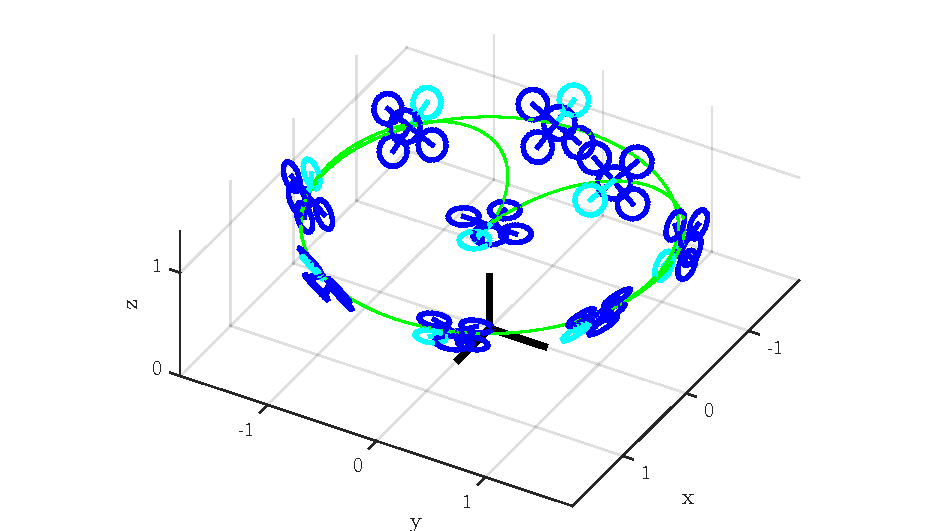
\includegraphics{QuadCircleTraj/QuadCircleTrajSnapshots}
%\\
% 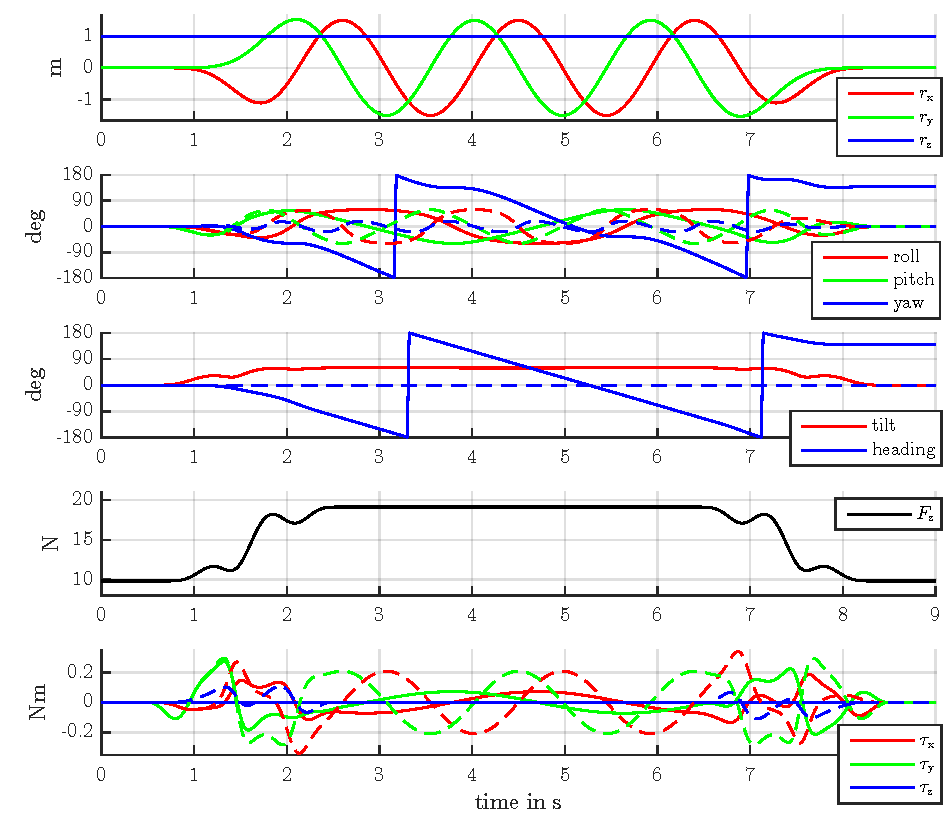
\includegraphics{QuadCircleTraj/QuadCircleTrajGraph}
% \caption{Example trajectory}
%\end{figure}



\subsection{Remote control input}
We use a standard remote control (FUTABA FX-35) with 8 analog channels and 6 switches, see \autoref{fig:RCchannels}.
On the multicopter side the receiver (FUTABA R6303SB) outputs the channels through the proprietary S.Bus which has been reverse engineered\footnote{\url{www.hackaday.com/2012/04/05/reverse-engineering-a-fubata-sbus-remote-control/}} to capture the channel values on the microcontroller.
The channels have a resolutions of $12\,\unit{Bit}$ and are sampled with $14\,\unit{ms}$.
The analog channels are scaled to the domain $-1 \leq \uRC[i] \leq 1, i=1\ldots,8$ and the switches to $\sRC[i] \in \{0,1,2\}, i=1,\ldots,6$.

%\begin{figure}[ht]
%\centering
% \input{graphics/RCchannels.pdf_tex}
% \caption{Remote control channels}
% \label{fig:RCchannels}
%\end{figure}

\paragraph{Derivative filtering.}
For the reference generation we need the derivatives of the analog RC inputs $\uRC$.
For this we implement the exact discretization (sampling time $\Ts=5\,\unit{ms}$) of a continuous filter of the from
\begin{align}
 \tdiff{t} \begin{bmatrix} \yRC[i] \\ \yRCd[i] \\ \yRCdd[i] \\ \yRCddd[i] \end{bmatrix}
 &= \begin{bmatrix} 0 & 1 & 0 & 0 \\ 0 & 0 & 1 & 0 \\ 0 & 0 & 0 & 1 \\ -a_0 & -a_1 & -a_2 & -a_3 \end{bmatrix}
 \begin{bmatrix} \yRC[i] \\ \yRCd[i] \\ \yRCdd[i] \\ \yRCddd[i] \end{bmatrix}
 + \begin{bmatrix} 0 \\ 0 \\ 0 \\ a_0 \end{bmatrix}
 \uRC[i],
\qquad 
 i = 1,\ldots,8.
\end{align}

The filter coefficients $a_i$ are chosen to resemble a (continuous) Bessel filter with cutoff frequency $7\,\unit{Hz}$, see e.g.\ \cite[sec.\,13.1.3]{TietzeSchenk:Halbleiter-Schaltungstechnik}.
A Bessel filter is characterized by having a maximally flat group delay, i.e.\ it preserves the (time-domain) shape of the signal in the passband (opposed to a Butterworth filter which preserves the amplitude in the frequency domain).
With rising order the (IIR) Bessel filter converges to a (FIR) Gaussian filter \cite[sec.\ 4.9.2]{Rabiner:DSP}.
\autoref{fig:RCFilter} shows the impulse response and application to a measured example RC-channel of the used Bessel filter and a corresponding Gaussian filter (windowlength 43).
Even though the difference is visible on the impulse response, the result of the implemented filter and the Gauss filter are indistinguishable in the application result.

%\begin{figure}[t]
% \centering
% 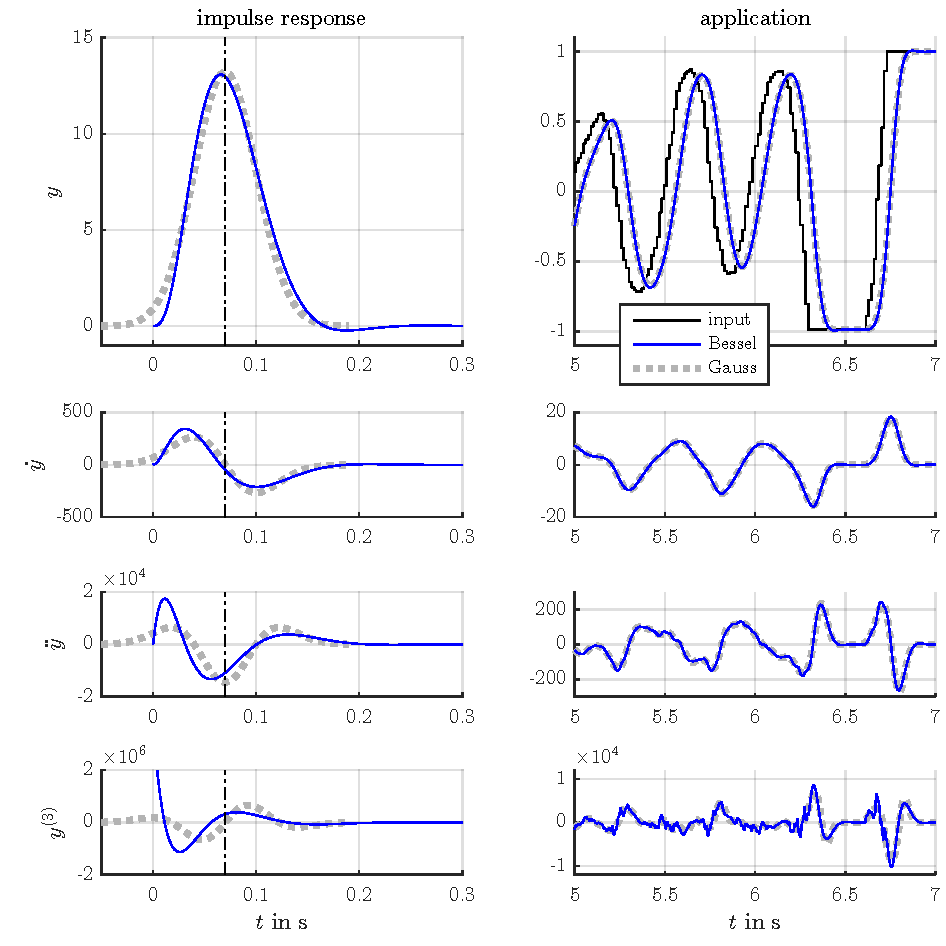
\includegraphics{RCFilter/RCFilter.pdf} 
% \caption{Application of the filter to the RC input}
% \label{fig:RCFilter}
%\end{figure}

The implemented filter is a trade-off between approximating the Gauss filter and being computationally cheap.

\subsection{Pilot mode}
In this mode the pilot commands the desired acceleration and attitude of the \Multicopter and 
\begin{align}
 \rRdd &= \RotMatZ(\headR) \accMax [\yRC[1], \yRC[2], \yRC[3]]^\top, 
\\
 \headRd &= \headRateMax \yRC[4],
\\
 \pRx &= \tiltMax \yRC[5], \ \pRy = \tiltMax \yRC[6],
\end{align}



\subsection{Trajectory generation modes}
\begin{itemize}
 \item Pilot mode without position control
 \begin{itemize}
  \item RC to acceleration in pilot frame
 \end{itemize}
 \item Pilot mode with position control
 \begin{itemize}
  \item RC to (integrated) position in pilot frame
 \end{itemize}
 \item Groundstation commands
 \begin{itemize}
  \item start polynomial transition to new position
  \item start precomputed trajectory
 \end{itemize}
\end{itemize}


%\begin{figure}[ht]
% \centering
% \input{graphics/IllustrateRCInputFrame.pdf_tex}
% \caption{Pilot reference frame}
% \label{fig:IllustrateRCInputFrame}
%\end{figure}


\paragraph{Transformation to reference signal.}
In pilot-mode only the remote control is used to interface with the multicopters.
One goal here is to establish an interface that works for the quadcopter \textit{and} the tricopter.

Firstly we only consider the outdoor operation where only the measurements from the IMU are available.
Here the body fixed force $F$ is computed from the RC inputs and the attitude $\R$ is actively controlled. 

To motivate the input scheme one has to put oneself into the pilots position:
The pilot knows the gravity $\vect{g}$ direction and sees the multicopter... \autoref{fig:IllustrateRCInputFrame}.
\begin{align}
 \rRdd = \RotMatZ(\headR) \pilotAccR
\qquad
 \RR = \RotMatZ(\headR)\, \RotMatPZ(\tiltCoeffR)
\end{align}
For the tricopter this yields the body fixed force
\begin{align}
 F_{\idxRef} = m \RRT (\rRdd - \gravityAcc) = m \RotMatPZ^\top(\tiltCoeffR) (\pilotAccR - \gravityAcc)
\end{align}



\begin{table}[ht]
\centering
\begin{tabular}{ccccc}
 \toprule
 quantity & scale & filter param & RC channel & comment\\
 \midrule
 $a_x$ & $\pm 3\,\sfrac{\unit{m}}{\unit{s}^2}$ & $70\,\unit{ms}$ & 1 \\
 $a_y$ & $\pm 3\,\sfrac{\unit{m}}{\unit{s}^2}$ & $70\,\unit{ms}$ & 0 \\
 $a_z$ & $\pm 3\,\sfrac{\unit{m}}{\unit{s}^2}$ & $70\,\unit{ms}$ & 2 \\
 $\dot{\varphi}$ & $\pm 60\,\sfrac{\unit{DEG}}{\unit{s}}$ & $150\,\unit{ms}$ & 3 \\
 $p_x$ & $\pm \sfrac{1}{3}$ & $150\,\unit{ms}$ & 10 & only tricopter \\
 $p_y$ & $\pm \sfrac{1}{3}$ & $150\,\unit{ms}$ & 11 & only tricopter \\
 \bottomrule
\end{tabular}
\caption{Pilot interface}
\label{tab:PilotInterface}
\end{table}


\subsection{Integral action for Quadcopter}
So far we have neglected the bias forces and torques $\FB$ and $\tauB$ for reference generation.
For the \Tricopter this is fine since they do not affect possible reference trajectories $t \mapsto (\rR, \RR)(t)$.
For any bias force and torque there is a control force that can counteract to it.

For the \Quadcopter the situation is different:
There are no control forces that directly counteract to $\FBx$ and $\FBy$.
Practically one can easily imagine that if the \Quadcopter should hover, $\rR=\const$, in the presence of a side wind it has to tilt to compensate it.
Mathematically this means that \eqref{eq:RefGenQuadcopterConstraint} is not valid for $\FBx, \FBy \neq 0$.

Introduce $\RR'$ and $\FRz'$ as the corrected reference that fulfill the translational dynamics in the presence of bias force
\begin{align}
 m(\rRdd-\gravityAcc) + d \rRd = \RR' (\FRz' \ez + \FB).
\end{align}
Set $\RR' = \RR P$, where $P\in \SpecialOrthogonalGroup(3)$ is the correction.
Using the properties of the nominal reference from \eqref{eq:RefGenQuadcopterConstraint} we can write
\begin{align}
 \underbrace{\RRT \big( m(\rRdd-\gravityAcc) + d \rRd \big)}_{\FRz \ez} = P (\FRz' \ez + \FB).
\end{align}
Decomposing this into magnitude and direction we have
\begin{align}\label{eq:RefGenQuadIntegralP}
 \FRz' = \sqrt{\FRz^2 - \FBx^2 - \FBy^2} - \FBz,
\qquad
 P^\top \ez = \tfrac{\FRz' \ez + \FB}{\FRz}.
\end{align}
This is a similar situation as discussed above for \eqref{eq:RefGenQuadcopterConstraint}: The relation \eqref{eq:RefGenQuadIntegralP} only fixes two of the three degrees of freedom of $P\in\SpecialOrthogonalGroup(3)$.
So we chose a similar solution
\begin{align}
 P^\top = \RotMatPZ\big( \tfrac{\FRz' \ez + \FB}{\FRz} \big).
\end{align}
This essentially is the solution of \eqref{eq:RefGenQuadIntegralP} for which the angle $\measuredangle P = \cos^{-1} \tfrac{1}{2}(\tr P - 1)$ is minimal.

By differentiation we get the corrected angular velocity $\wR' = \veeOp\big( (\RR P)^\top \tdiff{t}(\RR P)\big)$ and its derivative $\wRd'$.
This requires the assumption that the bias force is constant, $\FBd = 0$.

% For small bias force $\norm{\FB} \ll |\FRz|$ the corrections can be approximated as
% \begin{align}
%  \FRz' &= \FRz - \FBz + \mathcal{O}(\norm{\FB}^2),&
%  P &= \begin{bmatrix} 1 & 0 & -\tfrac{\FBx}{\FRz} \\ 0 & 1 & -\tfrac{\FBy}{\FRz} \\ \tfrac{\FBx}{\FRz} & \tfrac{\FBy}{\FRz} & 1 \end{bmatrix} + \mathcal{O}(\norm{\FB}^2).
% \end{align}

\section{Experimental results}
In this section finally discusses results of actual flight tests.
The task for the experiments is to track different reference trajectories while using the same controller and parameter values.
As the tracking errors for the following experiments were small, there was no distinguishable difference between the particle, body and energy based approaches.
The data for the presented figures were recorded while using the body based control approach.

The controller parameters for the following experiments are summarized in \autoref{tab:ParamTriQuadCtrl}.
Note that the values for inertia etc.\ are w.r.t.\ the body fixed frame and not w.r.t.\ the (closed loop) center of mass as done in \autoref{sec:CtrlExampleQuadcopter}.
Consequently the some values differ from what the matching conditions in \eqref{eq:CtrlExampleQuatMatchedParam} would suggest.

\begin{table}
 \centering
 \setlength{\tabcolsep}{.1em}
 \begin{tabular}{crlrll}
  \toprule
  \phantom{|} \quad symbol \quad\phantom{|} & \multicolumn{2}{c}{\phantom{|} \quad tricopter value \quad\phantom{|} } & \multicolumn{2}{c}{\phantom{|} \quad quadcopter value \quad\phantom{|}} & \multicolumn{1}{c}{\phantom{|} \qquad comment \qquad\phantom{|}} \\
  \midrule
  $\Ts$  & \multicolumn{4}{c}{$0.005\,\unit{s}$} & main sampling time \\
  \midrule
  $\quad\mc\quad$ & \phantom{|} \qquad$1.251$&$\unit{kg}$ & \phantom{|} \qquad$1.001$&$\unit{kg}$ & same as model \\
  $\scz$ & $ 0 $&$\unit{m}$ & $ 0.043$&$\unit{m}$ & center of mass \\
  $\Jcxx=\Jcyy$ & $0.0192$&$\unit{kg}\,\unit{m}^2$& $0.0095$&$\unit{kg}\,\unit{m}^2$ & tilt inertia \\
  $\Jczz$ & $0.0308$&$\unit{kg}\,\unit{m}^2$ & $0.0307$&$\unit{kg}\,\unit{m}^2$ & same as model 
  \\[.3ex]
  $\quad\dc\quad$ & $6$&$\tfrac{\unit{kg}}{\unit{s}}$ & $4.4$&$\tfrac{\unit{kg}}{\unit{s}}$ & translation damping \\
  $\lcz$ & $ 0 $&$\unit{m}$ & $ 0.255$&$\unit{m}$ & center of damping \\
  $\sigcxx=\sigcyy$ & $0.3$&$\tfrac{\unit{kg}\,\unit{m}^2}{\unit{s}}$& $0.4$&$\tfrac{\unit{kg}\,\unit{m}^2}{\unit{s}}$ & tilt damping \\
  $\sigczz$ & $0.25$&$\tfrac{\unit{kg}\,\unit{m}^2}{\unit{s}}$ & $0.1$&$\tfrac{\unit{kg}\,\unit{m}^2}{\unit{s}}$ & yaw damping
  \\[.3ex]
  $\quad\kc\quad$ & $8$&$\tfrac{\unit{kg}}{\unit{s}^2}$ & $8$&$\tfrac{\unit{kg}}{\unit{s}^2}$ & translation stiffness \\
  $\hcz$ & $ 0 $&$\unit{m}$ & $ 0.255$&$\unit{m}$ & center of stiffness \\
  $\kapcxx=\kapcyy$ & $1.7$&$\tfrac{\unit{kg}\,\unit{m}^2}{\unit{s}}$& $2.6$&$\tfrac{\unit{kg}\,\unit{m}^2}{\unit{s}}$ & tilt stiffness \\
  $\kapczz$ & $0.7$&$\tfrac{\unit{kg}\,\unit{m}^2}{\unit{s}}$ & $0.2$&$\tfrac{\unit{kg}\,\unit{m}^2}{\unit{s}}$ & yaw stiffness \\
  \midrule
  $\PropObsGainVel$  & \multicolumn{4}{c}{$0.1$} & propeller obs.\ gain 1 \\
  $\PropObsGainBias$  & \multicolumn{4}{c}{$0.01\,\unit{Hz}$} & propeller obs.\ gain 2 \\
  $\PropCtrlGain$  & \multicolumn{4}{c}{$0.25$} & propeller control gain \\
  $c_F$ & $0.1$& & & & thrust filter param \\
  $\omega_{\mathsf{mag}}$ & & & $100$&$\tfrac{\unit{RAD}}{\unit{s}}$ & thrust mag.\ bandwidth \\
  $\zeta_{\mathsf{mag}}$ & & & $0.707$& & thrust mag.\ damp.\ ratio \\
  $\omega_{\mathsf{tilt}}$ & & & $125$&$\tfrac{\unit{RAD}}{\unit{s}}$ & tilt torque bandwidth \\
  $\zeta_{\mathsf{tilt}}$ & & & $0.707$& & tilt torque damp.\ ratio \\
  $\omega_{\mathsf{head}}$ & & & $66$&$\tfrac{\unit{RAD}}{\unit{s}}$ & head.\ torque bandwidth \\
  \midrule
  $L_\omega$  & \multicolumn{4}{c}{$0.2$} & ang.\ vel.\ obs.\ gain \\
  $L_\tau$  & \multicolumn{4}{c}{$0.01$} & torque bias obs.\ gain \\
  $\cTPC$  & \multicolumn{4}{c}{$0.99$} & clock offset estimator root \\
  $l_r$  & \multicolumn{4}{c}{$1$} & pos.\ obs.\ fb.\ gain 1 \\
  $l_v$  & \multicolumn{4}{c}{$0.575$} & pos.\ obs.\ fb.\ gain 2 \\
  $l_a$  & \multicolumn{4}{c}{$-0.025$} & pos.\ obs.\ fb.\ gain 3 \\
  $l_F$  & \multicolumn{4}{c}{$0.01$} & force bias obs.\ fb.\ gain \\
  \bottomrule
 \end{tabular}
 \caption{Parameter values for tri- and quadcopter controller}
 \label{tab:ParamTriQuadCtrl}
\end{table}


\paragraph{Error quantization.}
In order to quantify the tracking performance we use the scalar quantities 
%position error $e_{\r}$, attitude error $e_{\R}$ and heading error $e_{\head}$ defined as
\begin{subequations}
\begin{align}
 e_{\r} &= \norm{\rObs - \rR},
\\
 e_{\R} &= \cos^{-1} \big( \tfrac{1}{2} (\tr\RE - 1) \big), \quad \RE = \RRT \RObs,
\\
 e_{\head} &= |\atanTwo(\REyx - \RExy, \RExx + \REyy)|.
\end{align} 
\end{subequations}
The position error $e_{\r}$ is the Euclidean distance between estimated position $\rObs$ and its reference $\rR$.
The attitude error $e_{\R}$ is the angle of the rotation matrix $\RE$ which rotates the reference attitude $\RR$ to the estimated attitude $\RObs$.
The heading error $e_{\head}$ is roughly the yaw angle of the error attitude $\RE$.

There are two reasons for considering the heading error $e_{\head}$ in addition to the attitude error $e_{\R}$:
Firstly the copters behave differently for the tilting degree of freedom and the heading.
This is also reflected by the different controller parameters for the respective directions.
Secondly, for the quadcopter, the tilting is used to compensate a horizontal position error.
A horizontal bias force implies a tilt error and consequently an attitude error.
%Based on the arguments from \autoref{sec:RealizationRefGenFlatness} one could say that the heading error $e_{\head}$ captures the part of the attitude error that is ``orthogonal'' to the tilt error.
Note that there is the relation $e_{\R} \geq e_{\head}$.

To quantify the errors for an experiment containing $N$ sampling steps we use the root-mean-square
\begin{align}
 \RMS(e_{\r}) = \sqrt{ \tfrac{1}{N} \textstyle{\sum_{k=1}^{N} \big( e_{\r}[k] \big)^2} }.
\end{align}
As an indicator for the dynamic of the reference trajectory for one experiment we consider the maximal velocity
\begin{align}
 \max(\norm{\vR}) = \max\big( \norm{\vR[1]}, \ldots, \norm{\vR[N]} \big)
\end{align}
and in the same way the maximal acceleration $\max(\norm{\vRd})$, the maximal angular velocity $\max(\norm{\wR})$ and the maximal angular acceleration $\max(\norm{\wRd})$.

The resulting values for the following four experiments are collected in \autoref{tab:MulticopterExperimentStatistics}.
Evidently, the quadcopter experiments are much more dynamic.
This is due to the fact that the quadcopter has a much better thrust to mass and torque to inertia ratio.

\begin{table}[htb]
 \centering
 \setlength{\tabcolsep}{.1em}
 \begin{tabular}{rlcccc}
  \toprule
   && \quad tricopter\quad & \quad quadcopter\quad & \quad quadcopter\quad & \quad quadcopter\quad \\
   && \quad transitions \quad & \quad transitions \quad & \quad looping \quad & \quad flip \quad \\
  \midrule
  $\max(\norm{\vR})$  &in $\tfrac{\unit{m}}{\unit{s}}$     & $2.2$   & $3.4$   & $4.2$   & $2.3$ \\[.5ex]
  $\max(\norm{\vRd})$ &in $\tfrac{\unit{m}}{\unit{s}^2}$   & $3.9$   & $8.2$   & $17.1$   & $17.5$ \\[.5ex]
%  $\max(\norm{\vRd})$ &in $\tfrac{\unit{m}}{\unit{s}^2}$   & $5.0$   & $8.2$   & $4.9$   & $7.8$ \\[.5ex]
  $\max(\norm{\wR})$  &in $\tfrac{\unit{deg}}{\unit{s}}$   & $318$   & $271$   & $537$   & $736$ \\[.5ex]
  $\max(\norm{\wRd})$ &in $\tfrac{\unit{deg}}{\unit{s}^2}$ & $497$   & $1380$  & $1610$  & $2480$ 
  \\[1ex]
  $\RMS(e_{\r})$      &in $\unit{m}$                       & $0.013$ & $0.017$ & $0.027$ & $0.026$ \\[.5ex]
  $\RMS(e_{\R})$      &in $\unit{deg}$                     & $1.1$   & $1.3$   & $2.5$   & $2.1$   \\[.5ex]
  $\RMS(e_{\head})$   &in $\unit{deg}$                     & $0.95$  & $0.3$   & $1.2$   & $0.8$   \\
  \bottomrule
 \end{tabular}
 \caption{Statistical values for the multicopter experiments}
 \label{tab:MulticopterExperimentStatistics}
\end{table}


\paragraph{Tricopter transitions.}
\autoref{fig:TriManeuver42Result} shows measurements of the tricopter tracking polynomial transitions between constant configurations.
A video of this experiment is available here\footnote{\url{https://youtu.be/oS5PHr6H0K4}}.

In the first $10\,\unit{s}$ the tricopter does some horizontal movement while maintaining the attitude and height.
For the next $10\,\unit{s}$ it tracks similar trajectories, but this time using the body tilt to generate the necessary horizontal force.
The difference between the approaches is obvious in the trajectories for the servo angles for the first case and the roll and pitch angle for the second case.
Furthermore a $90^\circ$ heading transition is added to the last two position transitions.
In the last third of the maneuver the tricopter tilts while maintaining its position.
One can see that for a body tilt of $15^\circ$ the servos have to tilt more than $30^\circ$.
The last transition is a $360^\circ$ heading rotation and $1\,\unit{m}$ height transition in $2\,\unit{s}$.
This is the part where we have the maximal attitude error of about $5^\circ$.
Here in particular one can see that the heading error $e_{\head}$ is the mayor part of the attitude error $e_{\R}$.

Comparing the performance of this tricopter experiment with the following quadcopter experiments, see \autoref{tab:MulticopterExperimentStatistics}, one can see that the tricopter has the lowest position and attitude error.
However, the comparison is not really fair since the quadcopter trajectories are much more dynamic.

\paragraph{Quadcopter transitions.}
\autoref{fig:QuadManeuver42Result} shows measurements of the quadcopter tracking polynomial transitions between constant configurations.
A video of this and the following experiments is available here\footnote{\url{https://youtu.be/x66sua3M6RQ}}.

The reference trajectories are very similar to the previous transitions for the tricopter, but with reduced transitions times.
The maximal velocity and acceleration, see \autoref{tab:MulticopterExperimentStatistics}, are achieved at about $12\,\unit{s}$, for a $2\,\unit{m}$ horizontal transition in $1.5\,\unit{s}$.
Since the tilt here is almost $45^\circ$ it is evident that the acceleration must be almost $\norm{\gravityAcc}$.
The last transition is a $360^\circ$ heading rotation in $4\,\unit{s}$, which is much slower as the corresponding maneuver for the tricopter due to the limited control torque of the quadcopter.
On the other hand the heading error $e_{\head}$ during this maneuver is much better as with the tricopter.
This might be a positive result of the sophisticated thrust controller from \autoref{sec:RealizationForceVectorControl}.

\paragraph{Quadcopter looping.}
\autoref{fig:QuadLoopResult} shows measurements of the quadcopter tracking four looping trajectories.
The reference trajectory for $\rx$ and $\rz$ is essentially a vertical circle with $2\,\unit{m}$ diameter, see \autoref{fig:introQuadLoopSnapshots}.
The individual looping takes about $3\,\unit{s}$ from rest to rest.

This is the first maneuver which involves that the quadcopter is upside down, i.e.\ $\RR \ez = -\ez$, so an appropriate method for the heading reference generation is required here.
Though the accelerations are quite high as well, this experiment has in comparison to the the others the highest translational velocity.
The fact that it has largest position and attitude errors could suggest that there are large model errors and/or unknown disturbances related to higher translational velocity.

% \begin{figure}
%  \centering
%  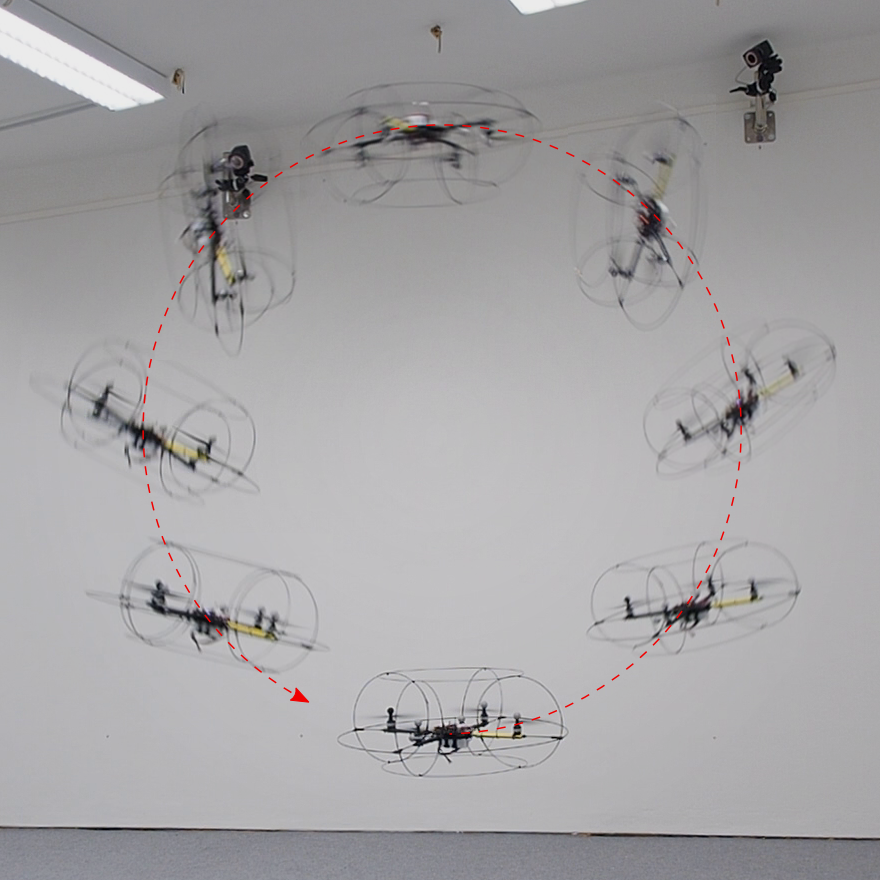
\includegraphics[width=.6\linewidth]{graphics/QuadLoopSnapshots.png}
%  \caption{Snapshots of the quadcopter tracking the loop trajectory}
%  \label{fig:QuadLoopSnapshots}
% \end{figure}

\paragraph{Quadcopter flip.}
\autoref{fig:QuadFlipResult} shows measurements of the quadcopter tracking six flip trajectories about different axis.
A flip is a trajectory where the quadcopter does a $360^\circ$ tilt transition while trying to minimize translational movement.
The maneuver here requires a vertical clearance of less than $1\,\unit{m}$ and just a few centimeters horizontally.
The individual flip takes less than $2\,\unit{s}$ from rest to rest.

This maneuver contains the largest translational and angular accelerations of the four experiments.
The maximal linear acceleration of $17.5\,\tfrac{\unit{m}}{\unit{s}^2}$ obviously appears when the quadcopter is upside down.
Here gravity pulls it with $9.81\,\tfrac{\unit{m}}{\unit{s}^2}$ and the propellers generate significant thrust in the same direction.

\begin{figure}
 \centering
 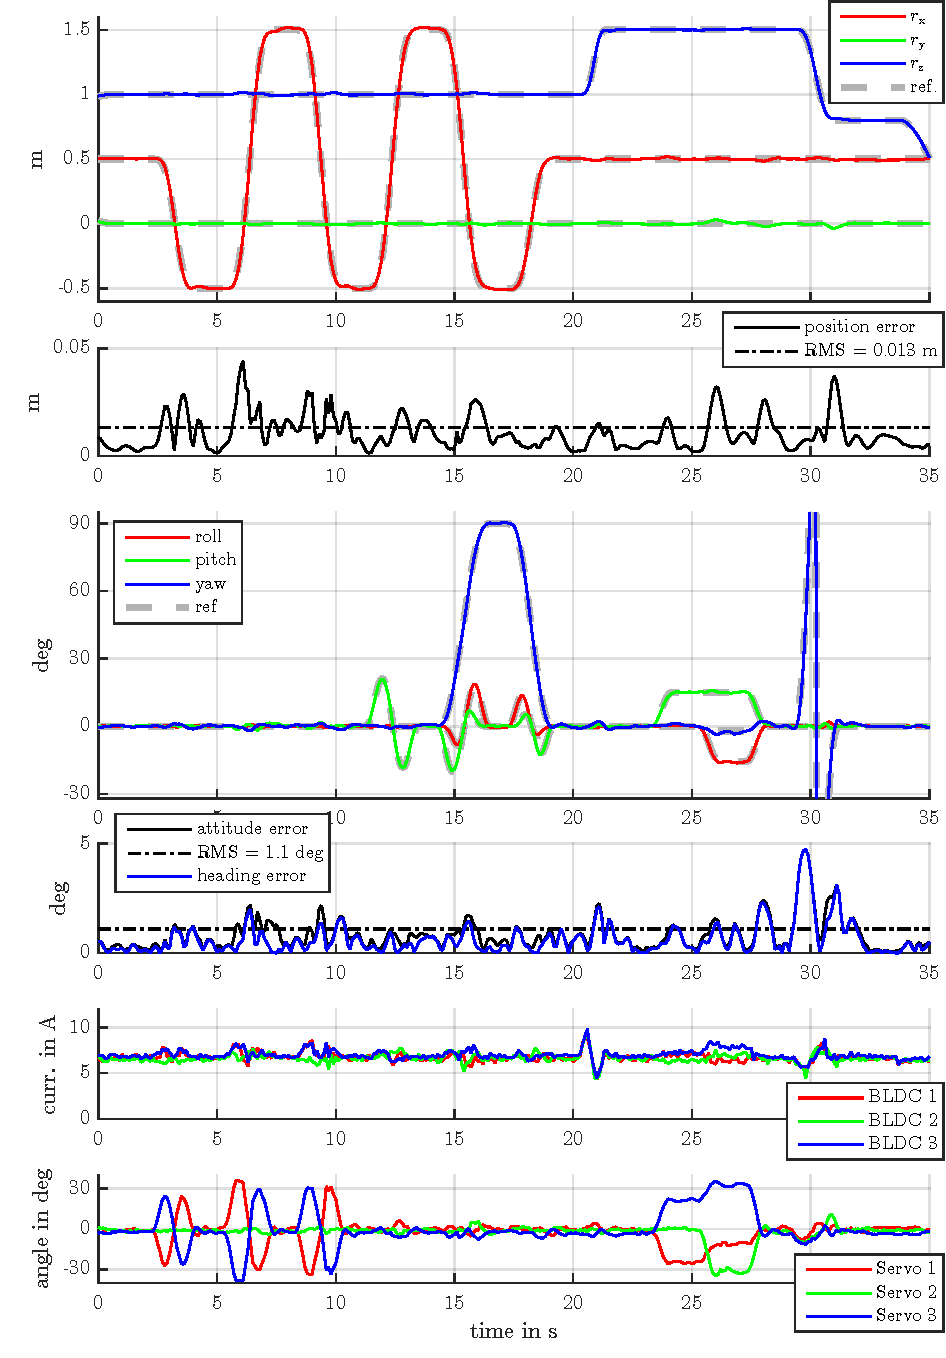
\includegraphics{graphics/TriFlightTest/TriManeuver42Result}
 \caption{Tricopter flight test result for polynomial transition trajectories}
 \label{fig:TriManeuver42Result}
\end{figure}

\begin{figure}
 \centering
 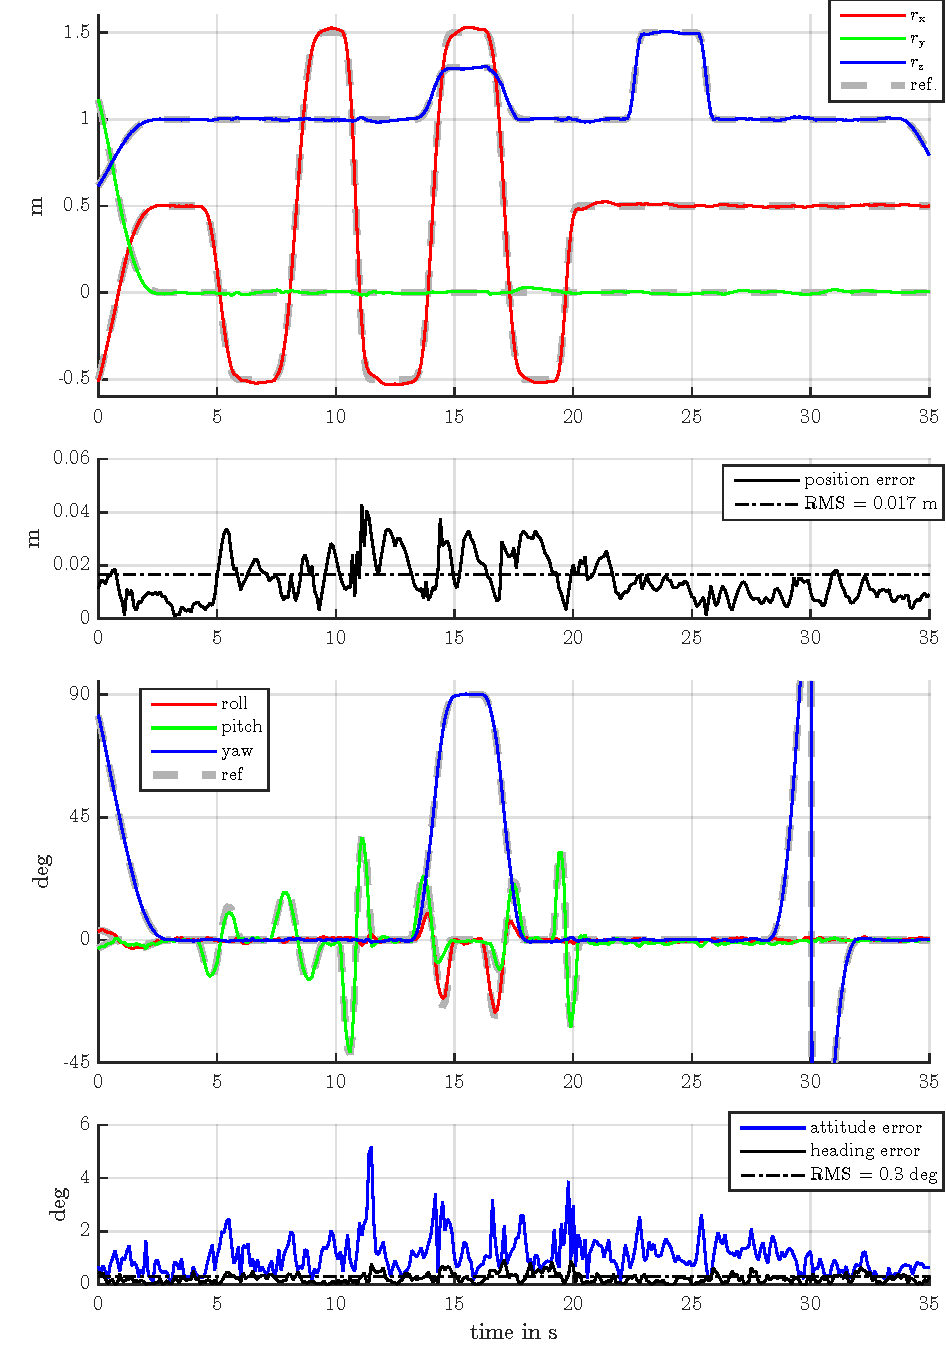
\includegraphics{graphics/QuadFlightTest/QuadManeuver42Result}
 \caption{Quadcopter flight test result for polynomial transition trajectories}
 \label{fig:QuadManeuver42Result}
\end{figure}

\begin{figure}
 \centering
 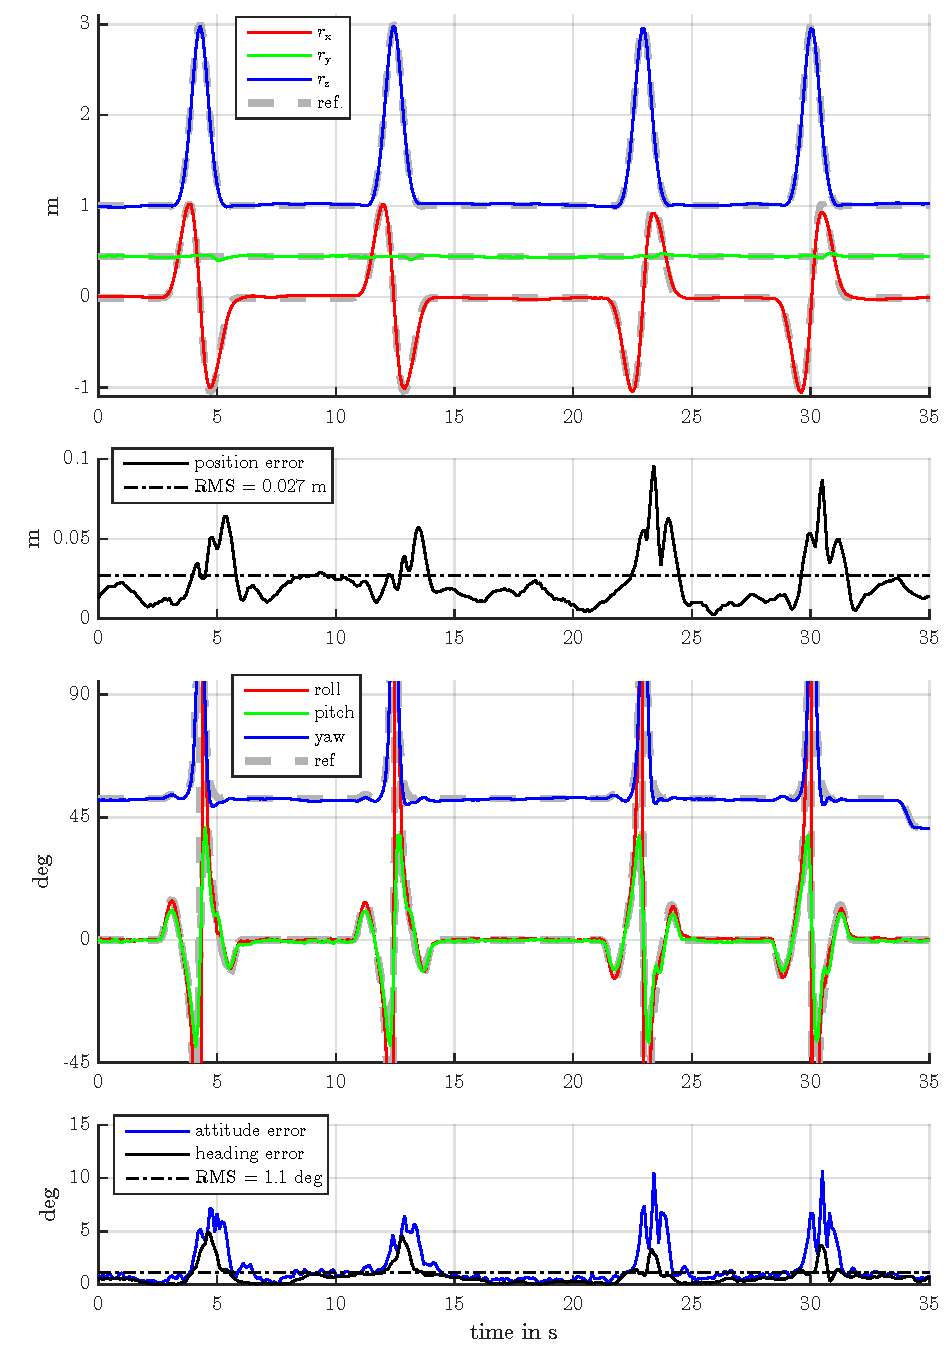
\includegraphics{graphics/QuadFlightTest/QuadLoopResult}
 \caption{Quadcopter flight test result for looping trajectories}
 \label{fig:QuadLoopResult}
\end{figure}

\begin{figure}
 \centering
 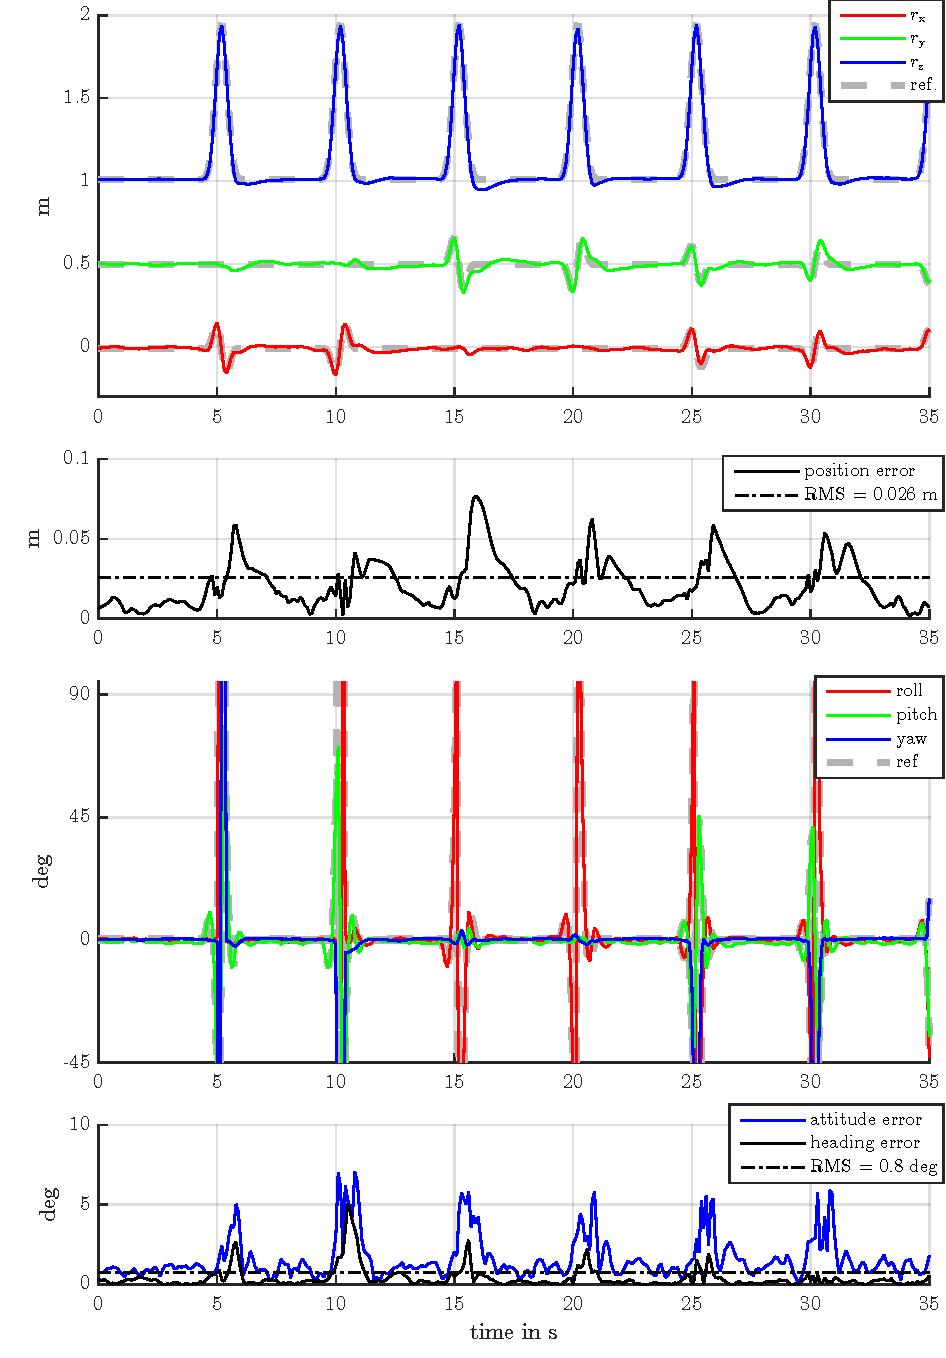
\includegraphics{graphics/QuadFlightTest/QuadFlipResult}
 \caption{Quadcopter flight test result for the flip trajectories}
 \label{fig:QuadFlipResult}
\end{figure}
% 
\chapter{Summary and Conclusions}

This work discussed the modeling and tracking control of rigid body systems.
Both subjects are well covered in the dedicated literature.
However, the literature is somewhat split into two viewpoints:
Small academic examples are treated independently with a lot of emphasis on the particular geometry like e.g. \cite{Marsden:MechanicsAndSymmetry}.
Larger multibody systems are handled by general formalisms, but treated by minimal generalized coordinates as if their configuration manifold is $\RealNum^\dimConfigSpace$ as in e.g.\ \cite{Schwertassek:MultibodySystems}.
This work attempts to combine both these points of view:
The proposed recipe for the equations of motion holds for general multibody systems \textit{and} allows a parameterization through redundant configuration coordinates that respect the underlying geometry of the system.

While inertia is arguably the core aspect of a rigid body system, this work also investigated into analog, natural stiffness and damping formulations.
The resulting damping and stiffness parameters, are not presented, maybe even unknown, in the dedicated literature.
The way e.g.\ the moment of stiffness matrix $\bodyMOS{}{}$ was derived here, it is just as natural as the (absolutely established) moment of inertia matrix $\bodyMOI{}{}$.

For control design, it is a common approach to design the desired closed loop dynamics and derive the actually required control law from it.
Flatness based control formalizes this approach but the vast majority combines it with linear error dynamics, thus treating the system as if its configuration manifold is $\RealNum^\numInputs$.
This work proposes desired closed loop dynamics based on a general mechanical model of a rigid body system.
As a result, the closed loop dynamics are invariant to the choice of coordinates in the same way as the motion of a mechanical system is unchanged by the choice of coordinates with which it is parameterized.
Furthermore, all control parameters have intrinsic mechanical interpretation, so should be intuitive for tuning.
 
Motivated by this basic idea, this work proposed three candidates for closed loop tracking dynamics:
One motivated by the dynamics of a particle system, one motivated by the rigid body energies and one motivated by the total energy of the system.
When dealing with the stabilization of a constant reference, the three approaches coincide and resemble an actual rigid body system subject to inertia, viscous damping and linear springs but not gravity.
For this case, the total energy is a Lyapunov function.
For tracking a general reference trajectory, only the third approach guarantees stability.
In contrast, this approach has the drawback of requiring an additional ingredient, the transport map, whose existence is not guaranteed.
Though not necessarily being a Lyapunov function, each approach comes with a formulation for a total energy that is positive definite, i.e.\ positive and zero if, and only if, the tracking objective is fulfilled, usually $\sysCoord=\sysCoordR$ and $\sysVel = \sysVelR$.

The three control approaches were applied to various examples of rigid body systems and tested in simulation with reasonable reference trajectories and initial conditions.
While the total energy was not always monotonically decreasing, it always eventually converged to zero.
So the general control objective was always achieved.

Finally, the proposed rigid body controller was successfully tested on the LSR-quad and tricopter.
The realization also required trajectory generation, state estimation and underlying actuator control which were each challenging control tasks in their on right.
From a coding perspective, the actual rigid body controller is less than 1\,\% of the microcontroller C code.
The presented experiments show the viability of the proposed control design in a practical environment with imperfect measurements and disturbances.
The quadcopter showed good tracking performance even while following aerobatic trajectories like loops and flips.

% \cite{Konz:Mathmod}
% \cite{Konz:Mathmod2018}
% \cite{Irscheid:HeavyRopesTricopter}
% \cite{Konz:GaussTrackingControl}
% \cite{Kastelan:Tricopter}
% \cite{Konz:Mechatronics}
% \cite{Konz:MechatronicsBook}


\appendix
\chapter{TBD} 
\section{On error coordinates}
\paragraph{Error coordinates.}
Introduce (possibly redundant) error coordinates $\sysCoordE \in \RealNum^{\numCoordE}$ as
\begin{align}
 \sysCoordE = \sysCoordFktE(\sysCoord, \sysCoordR), \qquad \geoConstraintE(\sysCoordE) = 0.
\end{align}
and require that this relation is invertible with $\sysCoord = \sysCoordFkt(\sysCoordE, \sysCoordR)$, i.e.\ $\sysCoordFkt(\sysCoordFktE(\sysCoord, \sysCoordR), \sysCoordR) = \sysCoord \, \forall \, \sysCoord \in \configSpace$.
The inverse function theorem now implies that the differential $\differential \sysCoordFktE = \pdiff[\sysCoordFktE]{\sysCoord} \kinMat $ has full rank: $\rank(\differential \sysCoordFktE) = \dim \configSpace = \dimConfigSpace$.

Let $\geoConstraintMatE$ be the linear independent rows of $\spdiff[\geoConstraintE]{\sysCoordE}$.
Then the derivative of the geometric constraint $\geoConstraintEd = 0$ implies
\begin{align}
 \geoConstraintMatE \differential \sysCoordFktE = 0,
\qquad
 \geoConstraintMatE \differentialR \sysCoordFktE = 0,
\end{align}
Since the matrices $\differential \sysCoordFktE$ and $\geoConstraintMatE$ have full rank, their pseudo-inverses are
\begin{align}
 (\differential \sysCoordFktE)^+ &= \big( (\differential \sysCoordFktE)^\top (\differential \sysCoordFktE) \big)^{-1} (\differential \sysCoordFktE)^\top,&
 (\differential \sysCoordFktE)^+ (\differential \sysCoordFktE) &= \idMat[\dimConfigSpace]
\\
 \geoConstraintMatE^+ &= \geoConstraintMatE^\top \big( \geoConstraintMatE \geoConstraintMatE^\top \big)^{-1},&
 \geoConstraintMatE \geoConstraintMatE^+ &= \idMat[\numCoordE - \dimConfigSpace].
\end{align}
Furthermore, due to the orthogonality $\geoConstraintMatE \differential \sysCoordFktE = 0$ we have
\begin{align}
 (\differential \sysCoordFktE) (\differential \sysCoordFktE)^+ + \geoConstraintMatE^+ \geoConstraintMatE = \idMat[\numCoordE].
\end{align}

\paragraph{Error potential.} 
We require that the potential $\potentialEnergyC$ can be expressed as a function $\potentialEnergyC_{\idxErr}$ of the error coordinates $\sysCoordE$ alone, i.e.\
\begin{align}
 \potentialEnergyC(\sysCoord, \sysCoordR) = \potentialEnergyC_{\idxErr}(\sysCoordFktE(\sysCoord, \sysCoordR)).
\end{align}
Now the requirement \eqref{eq:ReqTransportMap} for the transport map $\sysTransportMap$ can be written as
\begin{align}
 \differentialR \potentialEnergyC + \sysTransportMap^\top \differential \potentialEnergyC
 &= \big( \differentialR \sysCoordFktE + \differential \sysCoordFktE \sysTransportMap \big)^\top \pdiff[\potentialEnergyC_\idxErr]{\sysCoordE}
\nonumber\\
 &= \big( \underbrace{\big( (\differential \sysCoordFktE) (\differential \sysCoordFktE)^+ + \geoConstraintMatE^+ \geoConstraintMatE \big)}_{\idMat[\numCoordE]} \differentialR \sysCoordFktE + \differential \sysCoordFktE \sysTransportMap \big)^\top \pdiff[\potentialEnergyC_\idxErr]{\sysCoordE}
\nonumber\\
 &= \big( (\differential \sysCoordFktE)^+ (\differentialR \sysCoordFktE) +\,\sysTransportMap \big)^\top (\differential \sysCoordFktE)^\top \pdiff[\potentialEnergyC_\idxErr]{\sysCoordE}
 + \geoConstraintMatE^+ \underbrace{\geoConstraintMatE \differentialR \sysCoordFktE}_{0}  \pdiff[\potentialEnergyC_\idxErr]{\sysCoordE}
 = 0
\end{align}
which has the simple solution
\begin{align}\label{eq:DefErrorTransportMap}
 \sysTransportMap = -(\differential \sysCoordFktE)^+ (\differentialR \sysCoordFktE).
\end{align}

\paragraph{Error kinematics.}
With the same approach as above we can derive a kinematic relation between the error coordinates $\sysCoordE$ and the error velocity $\sysVelE = \sysVel - \sysTransportMap \sysVelR$ as
\begin{align}
 \sysCoordEd &= (\differential \sysCoordFktE) \sysVel + (\differentialR \sysCoordFktE) \sysVelR
\nonumber\\
 &= (\differential \sysCoordFktE) \sysVel + \underbrace{\big( (\differential \sysCoordFktE) (\differential \sysCoordFktE)^+ + \geoConstraintMatE^+ \geoConstraintMatE \big)}_{\idMat[\numCoordE]} \differentialR \sysCoordFktE \sysVelR
\nonumber\\
 &= (\differential \sysCoordFktE) \underbrace{\big( \sysVel + (\differential \sysCoordFktE)^+ (\differentialR \sysCoordFktE) \sysVelR \big)}_{\sysVelE}
 +\,\geoConstraintMatE^+ \underbrace{\geoConstraintMatE (\differentialR \sysCoordFktE)}_{0} \sysVelR
\end{align}

%\section{Linear algebra}

\subsection{Matrix sets}
Define the following sets of real matrices that are frequently used in the work: 
\begin{subequations}
\begin{align}
 &\text{(symmetric)}&
 \SymMat(n) &= \{ \mat{A} \in \RealNum^{n\times n} \, | \, \mat{A} = \mat{A}^\top \},
\\
 &\text{(symmetric, pos.\ def.)}&
 \SymMatP(n) &= \{ \mat{A} \in \SymMat(n) \, | \, \tuple{x}^\top\! \mat{A} \tuple{x} > 0 \, \forall \, \tuple{x} \in \RealNum^{n} \backslash \{\tuple{0}\} \},
\\
 &\text{(sym., pos.\ semi-def.)}&
 \SymMatSP(n) &= \{ \mat{A} \in \SymMat(n) \, | \, \tuple{x}^\top\! \mat{A} \tuple{x} \geq 0 \, \forall \, \tuple{x} \in \RealNum^{n} \backslash \{\tuple{0}\} \},
\\[2ex]
 &\text{(unit sphere)}&
 \mathbb{S}^n &= \{ \tuple{a} \in \RealNum^{n} \, | \, \tuple{a}^\top\tuple{a} = 1 \},
\\
 &\text{(orthogonal)}&
 \mathbb{O}(n) &= \{ \mat{A} \in \RealNum^{n\times n} \, | \, \mat{A}^{-1} = \mat{A}^\top \},
\\
 &\text{(special orthogonal)}&
 \SpecialOrthogonalGroup(n) &= \{ \mat{R} \in \mathbb{O}(n) \, | \, \det\mat{R} = +1 \},
\\
 &\text{(special Euclidean)}&
 \SpecialEuclideanGroup(n) &= \left\{ \begin{bmatrix} \R & \r \\ \mat{0} & 1 \end{bmatrix} \, \bigg| \, \r \in \RealNum^n, \R \in \SpecialOrthogonalGroup(n) \right\},
\\[2ex]
 &\text{(skew symmetric)}&
 \SpecialOrthogonalAlgebra(n) &= \{ \mat{\Omega} \in \RealNum^{n\times n} \, | \, \mat{\Omega}^\top = -\mat{\Omega} \},
\\
 &\text{}&
 \SpecialEuclideanAlgebra(n) &= \left\{ \begin{bmatrix} \mat{\Omega} & \tuple{v} \\ \mat{0} & 0 \end{bmatrix} \, | \, \mat{\Omega} \in \SpecialOrthogonalAlgebra(n), \tuple{v} \in \RealNum^{n} \right\}.
\end{align} 
\end{subequations}

\subsection{Trace}
The \textit{trace} of a quadratic matrix $\mat{A} \in \RealNum^{n\times n}$ is the sum of its diagonal entries
\begin{align}
 \tr \mat{A} = \sum_{i=1}^{n} A_{ii}
\end{align}
Some properties of the trace are
\begin{subequations}
\begin{align}
 \mat{A}, \mat{B} \in \RealNum^{n\times n}, \lambda\in\RealNum \,&:&
 \tr(\mat{A}+\mat{B}) &= \tr\mat{A} + \tr\mat{B},
\\
 &&
 \tr(\lambda \mat{A}) &= \lambda \tr\mat{A},
\\
 &&
 \tr \mat{A}^\top &= \tr \mat{A},
\\ 
 \mat{A} \in \RealNum^{n\times m}, \mat{B}\in\RealNum^{m\times n}\,&:&
 \tr(\mat{A}\mat{B}) &= \tr(\mat{B}\mat{A}),
\\ 
 \mat{A}, \mat{P} \in \RealNum^{n\times n}, \det\mat{P} \neq 0\,&:&
 \tr(\mat{P}^{-1} \mat{A} \mat{P}) &= \tr\mat{A}.
\\
 \mat{K}\in\SymMat(n), \mat{\Omega}\in\SpecialOrthogonalAlgebra(n)\,&:&
 \tr(\mat{K}\mat{\Omega}) &= 0.
\end{align}
\end{subequations}
For matrices $\mat{A},\mat{B}\in \RealNum^{n\times n}, n\geq2$ we may define the bijective mapping
\begin{align}
 \mat{B} = \tr(\mat{A})\idMat[n] - \mat{A}
\qquad \Leftrightarrow \qquad
 \mat{A} = \tfrac{1}{n-1}\tr(\mat{B}) \idMat[n] - \mat{B}.
\end{align}
which is due to $\tr\mat{B} = (n-1)\tr\mat{A}$.


\subsection{Inner product}\label{sec:MathInnerProduct}
\paragraph{Inner product.}
For matrices $\mat{A}, \mat{B} \in \RealNum^{n\times m}$ and a symmetric, positive definite matrix $ \mat{K} \in \SymMatP(n)$, define an \textit{inner product} as
\begin{align}\label{eq:DefMatrixInnerProduct}
 \sProd[\mat{K}]{\mat{A}}{\mat{B}} = \tr(\mat{A}^\top \mat{K} \mat{B}).
\end{align}
For $\mat{A}, \mat{B}, \mat{C} \in \RealNum^{n\times m}$ and $\lambda \in \RealNum$ we have the basic properties
\begin{subequations}
\begin{align}
 &\text{(linearity)}&
 \sProd[\mat{K}]{\lambda \mat{A}}{\mat{B}} &= \lambda \sProd[\mat{K}]{\mat{A}}{\mat{B}} = \sProd[\mat{K}]{\mat{A}}{\lambda \mat{B}},
\\
 &&
 \sProd[\mat{K}]{\mat{A}+\mat{C}}{\mat{B}} &= \sProd[\mat{K}]{\mat{A}}{\mat{B}} + \sProd[\mat{K}]{\mat{C}}{\mat{B}}
\\
 &\text{(symmetry)}&
 \sProd[\mat{K}]{\mat{B}}{\mat{A}} %&= \tr(B K A^\top) = \tr(A K^\top B^\top) = \tr(A K B^\top)
 &= \sProd[\mat{K}]{\mat{A}}{\mat{B}}
\\
 &\text{(positive definiteness)}&
 \sProd[\mat{K}]{\mat{A}}{\mat{A}} &\geq 0, \quad \sProd[\mat{K}]{\mat{A}}{\mat{A}} = 0 \ \Leftrightarrow \ \mat{A} = \mat{0}.
\end{align}
\end{subequations}
% Let $\tuple{a}_i$ and $\tuple{b}_i$ be the columns of $\mat{A}$ and $\mat{B}$, then
% \begin{align}
%  \sProd[\mat{K}]{\mat{A}}{\mat{B}} &= \tr \left( \begin{bmatrix} \tuple{a}_1^\top \\ \vdots \\ \tuple{a}_n^\top \end{bmatrix} \mat{K}  \big[ \tuple{b}_1 \cdots \tuple{b}_n \big] \right) 
%  = \tr \begin{bmatrix} \tuple{a}_1^\top \mat{K} \tuple{b}_1 & \cdots & \tuple{a}_1^\top \mat{K} \tuple{b}_n \\ \vdots & \ddots & \vdots \\ \tuple{a}_n^\top \mat{K} \tuple{b}_1 & \cdots & \tuple{a}_n^\top \mat{K} \tuple{b}_n \end{bmatrix} 
%  = \sum_{i=1}^n \tuple{a}_i^\top \mat{K} \tuple{b}_i.
% \end{align}
% With this the preceding properties should be clear.
Setting $\mat{K} = \idMat[n]$ in the definition \eqref{eq:DefMatrixInnerProduct} is called the \textit{Frobenius inner product} in \cite[sec.\ 5.2]{Horn:MatrixAnalysis} or \textit{Hilbert-Schmidt inner product} in \cite[sec.\ A.6]{Hall:LieGroups}.
Furthermore, for $\mat{A}, \mat{B} \in \RealNum^{n\times 1}$ it coincides with the common \textit{dot product}.

\paragraph{Norm.}
The induced norm is
\begin{align}
 \norm[\mat{K}]{\mat{A}} = \sqrt{\sProd[\mat{K}]{\mat{A}}{\mat{A}}}.
\end{align}
For $\mat{A}, \mat{B} \in \RealNum^{n\times m}$ and $\lambda \in \RealNum$ we have the basic properties
\begin{subequations}
\begin{align}
 &\text{(triangle inequality)}&
 \norm[\mat{K}]{\mat{A}+\mat{B}} &\leq \norm[\mat{K}]{\mat{A}} + \norm[\mat{K}]{\mat{B}}
\\
 &\text{(absolute homogeneity)}&
 \norm[\mat{K}]{\lambda \mat{A}} &= |\lambda| \, \norm[\mat{K}]{\mat{A}},
\\
 &\text{(positive definiteness)}&
 \norm[\mat{K}]{\mat{A}} &\geq 0, \quad \norm[\mat{K}]{\mat{A}} = 0 \ \Leftrightarrow \ \mat{A} = \mat{0}.
\end{align}
\end{subequations}

\paragraph{Metric.}
The induced metric is
\begin{align}
 d_{\mat{K}}(\mat{A}, \mat{B}) = \norm[\mat{K}]{\mat{A}-\mat{B}}.
\end{align}
For $\mat{A}, \mat{B}, \mat{C} \in \RealNum^{n\times m}$ and $\lambda \in \RealNum$ we have the basic properties
\begin{subequations}
\begin{align}
 &\text{(triangle inequality)}&
 \metric[\mat{K}]{\mat{A}}{\mat{B}} &\leq \metric[\mat{K}]{\mat{A}}{\mat{C}} + \metric[\mat{K}]{\mat{B}}{\mat{C}}
\\
 &\text{(symmetry)}&
 \metric[\mat{K}]{\mat{A}}{\mat{B}} &= \metric[\mat{K}]{\mat{B}}{\mat{A}},
\\
 &\text{(positive definiteness)}&
 \metric[\mat{K}]{\mat{A}}{\mat{B}} &\geq 0, \quad \metric[\mat{K}]{\mat{A}}{\mat{B}} = 0 \ \Leftrightarrow \ \mat{A} = \mat{B}.
\end{align}
\end{subequations}


\subsection{Vee \& wedge}
Define the $\wedOp$ operator for vectors as
\begin{subequations}\label{eq:AppDefWedgeOp}
\begin{align}
 \wedOp : \, \RealNum^3 \rightarrow \SpecialOrthogonalAlgebra(3) \, : \, \begin{bmatrix} \omega_1 \\ \omega_2 \\ \omega_3 \end{bmatrix} &\mapsto \begin{bmatrix} 0 & -\omega_3 & \omega_2 \\ \omega_3 & 0 & -\omega_1 \\ -\omega_2 & \omega_1 & 0 \end{bmatrix},&
\\
 \wedOp: \, \RealNum^6 \rightarrow \SpecialEuclideanAlgebra(3) \, : \ \ \begin{bmatrix} \v \\ \w \end{bmatrix} &\mapsto \begin{bmatrix} \wedOp\w & \v \\ \mat{0} & 0 \end{bmatrix},&
\end{align}
\end{subequations}
The corresponding inverse operator is denoted $\veeOp$.

Furthermore, define the $\veeTwoOp$ operator through
\begin{align}\label{eq:AppEqVeeTwo}
 \tr\big( \mat{A} (\wedOp\tuple{\xi})^\top \big) = \tuple{\xi}^\top \veeTwoOp(\mat{A}).
\end{align}
The particular important cases for this work are
\begin{subequations}\label{eq:AppDefVeeTwo}
\begin{align}
 \veeTwoOp &: \RealNum^{3\times 3} \rightarrow \RealNum^3 \, : \, \begin{bmatrix} \ast & A_{12} & A_{13} \\ A_{21} & \ast & A_{23} \\ A_{31} & A_{32} & \ast \end{bmatrix} \mapsto \begin{bmatrix} A_{32} - A_{23} \\ A_{13} - A_{31} \\ A_{21} - A_{12} \end{bmatrix},
\\
 \veeTwoOp &: \RealNum^{4\times 4} \rightarrow \RealNum^6 \, : \, \begin{bmatrix} \mat{A} & \tuple{b} \\ \ast & \ast \end{bmatrix} \mapsto \begin{bmatrix} \tuple{b} \\ \veeTwoOp\mat{A} \end{bmatrix}.
\end{align}
\end{subequations}
Note that for $\mat{\Omega} \in \SpecialOrthogonalAlgebra(3) \subset \RealNum^{3\times3}$ we have $\veeTwoOp(\mat{\Omega}) = 2 \veeOp(\mat{\Omega})$, thus giving the motivation for the name.

For matrices define the $\veeMatOp$ through the relation
\begin{align}\label{eq:AppEqVeeMat}
 \veeTwoOp\big(\wedOp(\tuple{\xi}) \, \mat{A} \big) = \veeMatOp(\mat{A}) \tuple{\xi}.
\end{align}
The particular important cases for this work are
\begin{subequations}\label{eq:AppDefVeeMat}
\begin{align}
 \veeMatOp &: \RealNum^{3\times 3} \rightarrow \RealNum^{3\times 3} \, : \, \mat{A} \mapsto \tr(\mat{A}) \idMat[3] - \mat{A},
\\
 \veeMatOp &: \RealNum^{4\times 4} \rightarrow \RealNum^{6\times 6} \, : \, \begin{bmatrix} \mat{A} & \tuple{b} \\ \tuple{c}^\top & d \end{bmatrix} \mapsto \begin{bmatrix} d \idMat[3] & (\wedOp \tuple{b})^\top \\ \wedOp\tuple{c} & \veeMatOp\mat{A} \end{bmatrix},
\end{align} 
\end{subequations}
The corresponding inverse operator is denoted $\wedMatOp$.
% \begin{align}
%  \mat{A}, \mat{P} \in \RealNum^{n\times n}, \det\mat{P} \neq 0\,:
% \qquad
%  \veeMatOp(\mat{P}^{-1} \mat{A} \mat{P}) = \mat{P}^{-1} \veeMatOp(\mat{A}) \mat{P}
% \end{align}
Combining \eqref{eq:AppEqVeeTwo} and \eqref{eq:AppEqVeeMat} yields
\begin{align}
 \tr\big( \wedOp\tuple{\xi}\, \mat{A} (\wedOp\tuple{\eta})^\top \big) = \tuple{\eta}^\top \veeMatOp(\mat{A}) \tuple{\xi}.
\end{align}

\section{SVD and polar decomposition}
\subsection{Singular value decomposition (SVD)}
Any matrix $\mat{A} \in \RealNum^{n\times m}$ can be decomposed into $\mat{A} = \mat{X} \mat{\varSigma} \mat{Y}^\top$, where $\mat{X} \in \OrthogonalGroup(n)$, $\mat{Y} \in \OrthogonalGroup(m)$ and $\mat{\varSigma} \in \RealNum^{n\times m}$ with $\varSigma_{ii} \geq 0, i=1,\ldots,\min(n,m), \varSigma_{ij} = 0, i\neq j$.
\begin{itemize}
 \item The columns of $\mat{X}$ are eigenvectors of $\mat{A} \mat{A}^\top = \mat{X} (\mat{\varSigma} \mat{\varSigma}^\top) \mat{X}^\top$.
 \item The columns of $\mat{Y}$ are eigenvectors of $\mat{A}^\top \mat{A} = \mat{Y} (\mat{\varSigma}^\top \mat{\varSigma}) \mat{Y}^\top$.
\end{itemize}
%The SVD is, in general, not unique.
It is common practice to place the singular values in descending order, i.e.\ $\varSigma_{ii} \geq \varSigma_{jj}, i > j$, thus making $\mat{\varSigma}$ unique.
The matrices $\mat{X}$ and $\mat{Y}$ are unique up to orthogonal transformations of the subspaces of each singular value and the kernel and co-kernel of $\mat{A}$.

\subsection{Polar decomposition}
Any square matrix $\mat{A} \in \RealNum^{n\times n}$ can be decomposed into $\mat{A} = \mat{U} \mat{K}$, where $\mat{U} \in \OrthogonalGroup(n)$, $\mat{K} \in \SymMatSP(n)$.
The matrix $\mat{K}$ is uniquely defined while $\mat{U}$ is only unique if $\mat{A}$ is invertible.
The same holds for the decomposition $\mat{A} = \mat{L} \mat{V}$, where $\mat{V} \in \OrthogonalGroup(n)$, $\mat{L} \in \SymMatSP(n)$.
The relation to the singular value decomposition $\mat{A} = \mat{X} \mat{\varSigma} \mat{Y}^\top$ is
\begin{align}
 \mat{U} = \mat{X} \mat{Y}^\top, \quad \mat{K} = \mat{Y} \mat{\varSigma} \mat{Y}^\top
\qquad \text{and} \qquad
 \mat{L} = \mat{X} \mat{\varSigma} \mat{X}^\top, \quad \mat{V} = \mat{X} \mat{Y}^\top.
\end{align}

\subsection{Special singular decomposition}
One problem when dealing with rigid body attitudes, i.e.\ $\SpecialOrthogonalGroup(3)$, is that the singular value decomposition and orthogonal decomposition return orthogonal matrices, i.e.\ $\det\mat{X}, \det\mat{Y} = \pm 1$, which might not be pure rotations.
A way to mend this was proposed in \cite{Kabsch:SSVD}:
Consider the SVD $\mat{A} = \mat{X} \mat{\varSigma} \mat{Y}^\top$ and define 
\begin{subequations}
\begin{align}
 \bar{\mat{X}} &= \mat{X} \diag(1, \ldots, 1, \det\mat{X}) \in \SpecialOrthogonalGroup(n),
\\
 \bar{\mat{Y}} &= \mat{Y} \diag(1, \ldots, 1, \det\mat{Y}) \in \SpecialOrthogonalGroup(n),
\\
 \bar{\mat{\varSigma}} &= \diag(\varSigma_{1,1}, \ldots, \varSigma_{n-1,n-1}, \varSigma_{n,n} \det\mat{X}\det\mat{Y}).
\end{align} 
\end{subequations}
i.e.\ flip the directions corresponding to the smallest singular value $\varSigma_{n,n}$ if the original orthonormal matrix contains a reflection.
We have a possibly different decomposition $\mat{A} = \bar{\mat{X}} \bar{\mat{\varSigma}} \bar{\mat{Y}}^\top$.

For the following we restrict to \textit{square matrices} $\mat{A}$ and consequently $\bar{\mat{\varSigma}}$.
Since $\bar{\varSigma}_{n,n} = \varSigma_{n,n} \det\mat{X}\det\mat{Y}$ might be negative, the matrix $\bar{\mat{\varSigma}}$ is, in general, indifferent.
Nevertheless, since only the smallest singular value might be flipped, the matrix $\veeMatOp(\bar{\mat{\varSigma}}) = \bar{\mat{\Lambda}}$ is positive semidefinite.

In the following we call $\mat{A} = \bar{\mat{X}} \wedMatOp(\bar{\mat{\varLambda}}) \bar{\mat{Y}}^\top$ with $\bar{\mat{X}}, \bar{\mat{Y}} \in \SpecialOrthogonalGroup(n)$ and $\bar{\mat{\varLambda}} \in \RealNum^{n\times n}$ with $\bar{\varLambda}_{ii} \geq 0, i=1,\ldots,n, \bar{\varLambda}_{ij} = 0, i\neq j$ the \textit{special} singular value decomposition.
Note that the property of the SVD $\bar{\varSigma}_{1,1} \geq \ldots \geq \bar{\varSigma}_{n-1,n-1} \geq |\bar{\varSigma}_{n,n}| \geq 0$ implies $\bar{\varLambda}_{1,1} \geq \ldots \geq \bar{\varLambda}_{n-1,n-1} \geq \bar{\varLambda}_{n,n} \geq 0$.
The uniqueness of $\bar{\mat{X}}, \bar{\mat{\varLambda}}, \bar{\mat{Y}}$ is the same as for the SVD.

\subsection{Special polar decomposition}
Using the special singular value decomposition above we may write
\begin{subequations}
\begin{align}
 \mat{A} 
 &= \bar{\mat{X}} \underbrace{\bar{\mat{Y}}^\top \bar{\mat{Y}}}_{\idMat[n]} \wedMatOp(\bar{\mat{\varLambda}}) \bar{\mat{Y}}^\top
 = \underbrace{\bar{\mat{X}} \bar{\mat{Y}}^\top}_{\mat{U}\,\in\,\SpecialOrthogonalGroup(n)} \wedMatOp\big(\underbrace{\bar{\mat{Y}} \bar{\mat{\varLambda}} \bar{\mat{Y}}^\top}_{\mat{K}\,\in\,\SymMatSP(n)}\big)
\\
 &= \bar{\mat{X}} \wedMatOp(\bar{\mat{\varLambda}}) \underbrace{\bar{\mat{X}}^\top \bar{\mat{X}}}_{\idMat[n]} \bar{\mat{Y}}^\top
 = \wedMatOp\big(\underbrace{\bar{\mat{X}} \bar{\mat{\varLambda}} \bar{\mat{X}}^\top}_{\mat{L}\,\in\,\SymMatSP(n)}\big) \underbrace{\bar{\mat{X}} \bar{\mat{Y}}^\top}_{\mat{U}\,\in\,\SpecialOrthogonalGroup(n)}
\end{align}
\end{subequations}
Since this only involves proper rotations this is potentially useful in physics where we cant have reflections.

These special versions of the singular value and polar decomposition are not established in the literature to the best of the authors knowledge.


\section{Attitude potential}\label{sec:AppendixAttitudePotential}
We are interested in the extrema of the function
\begin{align}
 \potentialEnergy(\R) = -\tr(\mat{P} \R), \quad \R \in \SpecialOrthogonalGroup(3)
\end{align}
with the constant parameter $\mat{P} \in \RealNum^{3\times3}$.
Similar functions appear in the context of attitude control \cite{Koditschek:TotalEnergy} or in the so-called Wahba's problem \cite{Wahba:WahbaProblem}.

\paragraph{Coordinate transformation.}
A crucial ingredient for the solution is what we called the \textit{special singular value decomposition} above:
Let $\mat{P} = \bar{\mat{X}} \wedMatOp(\mat{\varLambda}) \bar{\mat{Y}}^\top$ with $\bar{\mat{X}}, \bar{\mat{Y}} \in \SpecialOrthogonalGroup(3)$ and $\mat{\varLambda} = \diag(\lambda_1, \lambda_2, \lambda_3)$, $\lambda_1 \geq \lambda_2 \geq \lambda_3 \geq 0$.
With this we define the transformed function
\begin{align}
 \potentialEnergy(\R) = -\tr( \bar{\mat{X}} \wedMatOp(\mat{\varLambda}) \bar{\mat{Y}}^\top \R) = -\tr( \wedMatOp(\mat{\varLambda}) \underbrace{\bar{\mat{Y}}^\top \R \bar{\mat{X}}}_{\bar{\R}}) =: \bar{\potentialEnergy}(\bar{\R})
\end{align}
Since the SVD is not unique in general, the transformed function $\bar{\potentialEnergy}$ is neither.
However, since the coordinate transformation $\R = \bar{\mat{Y}} \bar{\R} \bar{\mat{X}}^\top$ is bijective, no information is lost here.
% The SVD is also the most robust approach for the numerical solution of the problem \cite{Markley:Wahba}.

\paragraph{Critical points.}
The first and second differential of the transformed function are
\begin{align}
 \differential \bar{\potentialEnergy}(\bar{\R}) &= \veeTwoOp(\wedMatOp(\mat{\varLambda}) \bar{\R}),
\\
 \differential^2 \bar{\potentialEnergy}(\bar{\R}) &= \veeMatOp(\wedMatOp(\mat{\varLambda}) \bar{\R})^\top.
\end{align}
So, for a critical point $\bar{\R}_0 : \differential \bar{\potentialEnergy}(\bar{\R}_0)=\tuple{0}$ we need the matrix $\wedMatOp(\mat{\varLambda}) \bar{\R}_0$ to be symmetric.
An obvious critical point is $\bar{\R}_0 = \idMat[3]$ which is a minimum if $\differential^2 \bar{\potentialEnergy}(\idMat[3]) = \mat{\varLambda}$ is positive definite.
Depending on the actual constellation of $\lambda_1 \geq \lambda_2 \geq \lambda_3 \geq 0$ we have more critical points or submanifolds which are analysed in the following:
\begin{subequations}
\begin{itemize}
\item Distinct eigenvalues: $\lambda_3 > \lambda_2 > \lambda_1 > 0$: We have the critical points
\begin{align}
 &\bar{\R}_{0} = \idMat[3] \ :
\nonumber\\
 &\quad
 \potentialEnergy(\bar{\R}_{0}) = -\tfrac{\lambda_1}{2} - \tfrac{\lambda_2}{2} - \tfrac{\lambda_3}{2}, 
 \quad
 \eig(\differential^2 \bar{\potentialEnergy}(\bar{\R}_{0})) = \{ \lambda_3, \lambda_2, \lambda_1 \}
\\
 &\bar{\R}_{1} = \diag(1,-1,-1) \ :
\nonumber\\
 &\quad
 \potentialEnergy(\bar{\R}_{1}) = \tfrac{3\lambda_1 - \lambda_2 - \lambda_3}{2}, 
 \quad
 \eig(\differential^2 \bar{\potentialEnergy}(\bar{\R}_{1})) = \{ \lambda_3-\lambda_1, \lambda_2-\lambda_1, -\lambda_1 \}
\\
 &\bar{\R}_{2} = \diag(-1,1,-1) \ :
\nonumber\\
 &\quad
 \potentialEnergy(\bar{\R}_{2}) = \tfrac{3\lambda_2 - \lambda_1 - \lambda_3}{2}, 
 \quad
 \eig(\differential^2 \bar{\potentialEnergy}(\bar{\R}_{2})) = \{ \lambda_3-\lambda_2, \lambda_1-\lambda_2, -\lambda_2 \}
\\
 &\bar{\R}_{3} = \diag(-1,-1,1) \ :
\nonumber\\
 &\quad
 \potentialEnergy(\bar{\R}_{3}) = \tfrac{3\lambda_3 - \lambda_1 - \lambda_2}{2}, 
 \quad
 \eig(\differential^2 \bar{\potentialEnergy}(\bar{\R}_{3})) = \{ \lambda_2-\lambda_3, \lambda_1-\lambda_3, -\lambda_3 \}
\end{align}
so $\bar{\R}_{0}$ is a minimum, $\bar{\R}_{1}$ and $\bar{\R}_{2}$ are saddle points, and $\bar{\R}_{3}$ is a maximum.

\item Double eigenvalue: $\lambda_3 > \lambda_2 = \lambda_1 > 0$: We have a minimum at $\bar{\R}_{0}$, a maximum at $\bar{\R}_{3}$ and a saddle on the circular manifold 
\begin{align}
 \bar{\R}_{4} &= \begin{bmatrix} -c & s & 0 \\ s & c & 0 \\ 0 & 0 & -1 \end{bmatrix}, \ c^2+s^2=1 \ : 
\nonumber\\
 &\quad
 \potentialEnergy(\bar{\R}_{4}) = \lambda_1 - \tfrac{\lambda_3}{2}, 
 \quad
 \eig(\differential^2 \bar{\potentialEnergy}(\bar{\R}_{4})) = \{ \lambda_3-\lambda_1, 0, -\lambda_1 \}
\end{align}
which includes the points $\bar{\R}_{1}$ and $\bar{\R}_{2}$.

\item Double eigenvalue: $\lambda_3 = \lambda_2 > \lambda_1 > 0$: Analog to above we have a minimum at $\bar{\R}_{0}$, a saddle at $\bar{\R}_{4}$ and a maximum on the circular manifold 
\begin{align}
 \bar{\R}_{5} &= \begin{bmatrix} -1 & 0 & 0 \\ 0 & c & s \\ 0 & s & -c \end{bmatrix}, \ c^2+s^2=1 \ : 
\nonumber\\
 &\quad
 \potentialEnergy(\bar{\R}_{5}) = \lambda_2 - \tfrac{\lambda_1}{2}, 
 \quad
 \eig(\differential^2 \bar{\potentialEnergy}(\bar{\R}_{5})) = \{ 0, \lambda_1-\lambda_2, -\lambda_2 \}
\end{align}
which includes the points $\bar{\R}_{2}$ and $\bar{\R}_{3}$.

\item Triple eigenvalue: $\lambda_3 = \lambda_2 = \lambda_1 > 0$: Minimum at $\bar{\R}_{0}$ and a maximum on the spherical manifold 
\begin{align}
 &\bar{\R}_{6} = \begin{bmatrix} \quatx^2 - \quaty^2 - \quatz^2 & 2\quatx\quaty & 2\quatx\quatz \\ 2\quatx\quaty & \quaty^2-\quatx^2+\quatz^2 & 2\quaty\quatz \\ 2\quatx\quatz & 2\quaty\quatz & \quatz^2-\quatx^2-\quaty^2 \end{bmatrix}, \ \quatx^2+\quaty^2+\quatz^2=1 :
\nonumber\\
 &\quad
 \potentialEnergy(\bar{\R}_{6}) = \tfrac{\lambda_1}{2},
 \quad
 \eig(\differential^2 \bar{\potentialEnergy}(\bar{\R}_{6})) = \{ 0, 0, -\lambda_1 \}
\end{align}
which includes the points $\bar{\R}_{1}$, $\bar{\R}_{2}$ and $\bar{\R}_{3}$ and the circles $\bar{\R}_4$ and $\bar{\R}_5$.
It corresponds to a $180^\circ$ rotation about an arbitrary axis $[\quatx,\quaty,\quatz]^\top \in \Sphere^2$.

\item One zero eigenvalue: $\lambda_3 > \lambda_2 > \lambda_1 = 0$: We have a minimum on the circular manifold
\begin{align}
 \bar{\R}_{7} &= \begin{bmatrix} 1 & 0 & 0 \\ 0 & c & -s \\ 0 & s & c \end{bmatrix}, \ c^2+s^2=1 \ : 
\nonumber\\
 \potentialEnergy(\bar{\R}_{7}) &= -\tfrac{\lambda_2+\lambda_3}{2}, \qquad
 \eig(\differential^2 \bar{\potentialEnergy}(\bar{\R}_{7})) = \{ \lambda_3, \lambda_2, 0\}
\end{align}
which includes $\bar{\R}_{0}$ and $\bar{\R}_{1}$.
Furthermore we have a saddle point at $\bar{\R}_{2}$ and a maximum at $\bar{\R}_{3}$.

\item Double eigenvalue and zero eigenvalue: $\lambda_3 = \lambda_2 > \lambda_1 = 0$: We have a minimum on $\bar{\R}_{7}$ and a maximum on $\bar{\R}_{5}$.

\item Two zero eigenvalues: $\lambda_3 > \lambda_2 = \lambda_1 = 0$: We have a minimum on the spherical manifold
\begin{align}
 \bar{\R}_{8} &= \begin{bmatrix} \quatw^2 + \quatx^2 - \quaty^2 & 2\quatx\quaty & 2\quatw\quaty \\ 2\quatx\quaty & \quatw^2-\quatx^2+\quaty^2 & -2\quatw\quatx \\ -2\quatw\quatx & 2\quatw\quatx & \quatw^2-\quatx^2-\quaty^2 \end{bmatrix}, \ \quatw^2+\quatx^2+\quaty^2=1 :
\nonumber\\
 \potentialEnergy(\bar{\R}_{8}) &= -\tfrac{\lambda_3}{2}, \qquad
 \eig(\differential^2 \bar{\potentialEnergy}(\bar{\R}_{8})) = \{ \lambda_3, 0, 0\}
\end{align}
which includes $\bar{\R}_{0}$, $\bar{\R}_{1}$ and $\bar{\R}_{2}$ and corresponds to an arbitrary rotation about an axis $[\quatx, \quaty, 0]^\top$.
Furthermore we have a maximum at $\bar{\R}_{3}$.

\item All zero Eigenvalues: $\lambda_3 = \lambda_2 = \lambda_1 = 0$: for this we have $\bar{\mat{\varSigma}} = \mat{P} = \mat{0}$ and the function is $\potentialEnergy = 0$.

\end{itemize}
\end{subequations}
We may conclude that the function $\bar{\potentialEnergy}$ has a minimum at $\bar{\R}_0 = \idMat[3]$ and a maximum at $\bar{\R}_3 = \diag(-1,-1,1)$, though they may not be strict.
The minimum is strict if and only if $\lambda_1 > 0$. 
The maximum is strict if and only if $\lambda_3>\lambda_2$.

It should also be noted that the results of this paragraph would be much more ``symmetric'' if we would not have required the descending order of the singular values $\sigma_i$.
This did however reduce the number of cases to distinguish.

\paragraph{Original coordinates.}
The original function $\potentialEnergy$ has a minimum at $\R_0 = \bar{\mat{Y}} \bar{\mat{X}}^\top$.
% We may decompose
% \begin{align}
%  \mat{P}
%  = \bar{\mat{X}} \bar{\mat{\varSigma}} \bar{\mat{Y}}^\top 
%  = \bar{\mat{X}} \wedMatOp(\mat{\Lambda}) \underbrace{\bar{\mat{X}}^\top \bar{\mat{X}}}_{\idMat[3]} \bar{\mat{Y}}^\top
%  = \wedMatOp( \underbrace{\bar{\mat{X}} \mat{\Lambda} \bar{\mat{X}}^\top }_{\mat{K}}) \R_0^\top
% \end{align}
% with $\mat{K} \in \SymMatSP(3)$.
The minimum $\R_0$ is strict, if, and only if, $\lambda_i > 0, i=1,2,3$ or equivalently if $\mat{K}$ is positive definite:
\begin{align}
 \mat{K} = \differential^2 \potentialEnergy (\R_0) = \veeMatOp(\mat{P}\R_0) = \bar{\mat{X}} \mat{\Lambda} \bar{\mat{X}}^\top.
\end{align}
Note that the minimum $\R_0$ and the Hessian $\mat{K}$ coincide with the special orthogonal decomposition $\mat{P}^\top = \R_0 \wedMatOp(\mat{K})$ introduced above.

\paragraph{Prototype for a positive definite function.}
Substracting the minimal value $\potentialEnergy(\R_0)$ from the function we obtain
\begin{subequations}
\begin{align}
 \hat{\potentialEnergy}(\R) &= \potentialEnergy(\R) - \potentialEnergy(\R_0)
\nonumber\\
 &= -\tr(\bar{\mat{X}} \wedMatOp(\mat{\Lambda}) \bar{\mat{Y}}^\top \R) + \tfrac{1}{2}\tr(\mat{\Lambda})
\nonumber\\
 &= -\tr(\bar{\mat{X}} \wedMatOp(\mat{\Lambda}) \bar{\mat{X}}^\top \R_0^\top \R) + \tr(\wedMatOp(\mat{K}))
\nonumber\\
\label{eq:NavFunctionSO3}
 &= \tr\big(\wedMatOp(\mat{K})(\idMat[3] - \R_0^\top \R)\big)
\\
 &= \tfrac{1}{2} \tr\big(\wedMatOp(\mat{K})(\R - \R_0)^\top (\R - \R_0)\big)
\nonumber\\
 &= \tfrac{1}{2}\norm[\wedMatOp(\mat{K})]{\R-\R_0}^2.
\end{align}
\end{subequations}
We have the properties
\begin{subequations}
\begin{align}
 \mat{K} &\geq 0& 
 &\Leftrightarrow&
 \hat{\potentialEnergy}(\R) &\geq 0
\\
 \mat{K} &> 0& 
 &\Leftrightarrow&
 \hat{\potentialEnergy}(\R) &\geq 0 \ \wedge \ \hat{\potentialEnergy}(\R) = 0 \, \Leftrightarrow \, \R = \R_0.
\end{align}
\end{subequations}
The form \eqref{eq:NavFunctionSO3} is called the \textit{navigation function} for $\SpecialOrthogonalGroup(3)$ in \cite{Koditschek:TotalEnergy}.
From its properties $\hat{\potentialEnergy}$ is an $\SpecialOrthogonalGroup(3)$ analogon to $\tfrac{1}{2}(\tuple{x}-\tuple{x}_0)^\top\mat{K}(\tuple{x}-\tuple{x}_0), \tuple{x},\tuple{x}_0\in\RealNum^3$.
 
% \section{Linear Algebra}
% \paragraph{Normal matrix}
% A square matrix $\mat{A} \in \RealNum^{n\times n}$ is called \textit{normal} if $\mat{A}^\top \mat{A} = \mat{A} \mat{A}^\top$.
% A normal matrix is diagonalizable by a orthonormal matrix. 

\subsection{Matrix sets}
Define the following sets of real matrices that are frequently used in the work: 
\begin{subequations}
\begin{align}
 &\text{(symmetric)}&
 \SymMat(n) &= \{ \mat{A} \in \RealNum^{n\times n} \, | \, \mat{A} = \mat{A}^\top \},
\\
 &\text{(symmetric, pos.\ def.)}&
 \SymMatP(n) &= \{ \mat{A} \in \SymMat(n) \, | \, \tuple{x}^\top\! \mat{A} \tuple{x} > 0 \, \forall \, \tuple{x} \in \RealNum^{n} \backslash \{\tuple{0}\} \},
\\
 &\text{(sym., pos.\ semi-def.)}&
 \SymMatSP(n) &= \{ \mat{A} \in \SymMat(n) \, | \, \tuple{x}^\top\! \mat{A} \tuple{x} \geq 0 \, \forall \, \tuple{x} \in \RealNum^{n} \backslash \{\tuple{0}\} \},
\\[2ex]
 &\text{(unit sphere)}&
 \mathbb{S}^n &= \{ \tuple{a} \in \RealNum^{n} \, | \, \tuple{a}^\top\tuple{a} = 1 \},
\\
 &\text{(orthogonal)}&
 \mathbb{O}(n) &= \{ \mat{A} \in \RealNum^{n\times n} \, | \, \mat{A}^{-1} = \mat{A}^\top \},
\\
 &\text{(special orthogonal)}&
 \SpecialOrthogonalGroup(n) &= \{ \mat{R} \in \mathbb{O}(n) \, | \, \det\mat{R} = +1 \},
\\
 &\text{(special Euclidean)}&
 \SpecialEuclideanGroup(n) &= \left\{ \begin{bmatrix} \R & \r \\ \mat{0} & 1 \end{bmatrix} \, \bigg| \, \r \in \RealNum^n, \R \in \SpecialOrthogonalGroup(n) \right\},
\\[2ex]
 &\text{(skew symmetric)}&
 \SpecialOrthogonalAlgebra(n) &= \{ \mat{\Omega} \in \RealNum^{n\times n} \, | \, \mat{\Omega}^\top = -\mat{\Omega} \},
\\
 &\text{}&
 \SpecialEuclideanAlgebra(n) &= \left\{ \begin{bmatrix} \mat{\Omega} & \tuple{v} \\ \mat{0} & 0 \end{bmatrix} \, | \, \mat{\Omega} \in \SpecialOrthogonalAlgebra(n), \tuple{v} \in \RealNum^{n} \right\}.
\end{align} 
\end{subequations}

\subsection{Trace}
The \textit{trace} of a quadratic matrix $\mat{A} \in \RealNum^{n\times n}$ is the sum of its diagonal entries
\begin{align}
 \tr \mat{A} = \sum_{i=1}^{n} A_{ii}
\end{align}
Some properties of the trace are
\begin{subequations}
\begin{align}
 \mat{A}, \mat{B} \in \RealNum^{n\times n}, \lambda\in\RealNum \,&:&
 \tr(\mat{A}+\mat{B}) &= \tr\mat{A} + \tr\mat{B},
\\
 &&
 \tr(\lambda \mat{A}) &= \lambda \tr\mat{A},
\\
 &&
 \tr \mat{A}^\top &= \tr \mat{A},
\\ 
 \mat{A} \in \RealNum^{n\times m}, \mat{B}\in\RealNum^{m\times n}\,&:&
 \tr(\mat{A}\mat{B}) &= \tr(\mat{B}\mat{A}),
\\ 
 \mat{A}, \mat{P} \in \RealNum^{n\times n}, \det\mat{P} \neq 0\,&:&
 \tr(\mat{P}^{-1} \mat{A} \mat{P}) &= \tr\mat{A}.
\\
 \mat{K}\in\SymMat(n), \mat{\Omega}\in\SpecialOrthogonalAlgebra(n)\,&:&
 \tr(\mat{K}\mat{\Omega}) &= 0.
\end{align}
\end{subequations}
For matrices $\mat{A},\mat{B}\in \RealNum^{n\times n}, n\geq2$ we may define the bijective mapping
\begin{align}
 \mat{B} = \tr(\mat{A})\idMat[n] - \mat{A}
\qquad \Leftrightarrow \qquad
 \mat{A} = \tfrac{1}{n-1}\tr(\mat{B}) \idMat[n] - \mat{B}.
\end{align}
which is due to $\tr\mat{B} = (n-1)\tr\mat{A}$.


\subsection{Vee \& wedge operatos}
Define
\begin{subequations}%\label{eq:DefWedgeOp}
\begin{align}
 \wedOp : \, \RealNum^3 \rightarrow \SpecialOrthogonalAlgebra(3) \, : \, \begin{bmatrix} \omega_1 \\ \omega_2 \\ \omega_3 \end{bmatrix} &\mapsto \begin{bmatrix} 0 & -\omega_3 & \omega_2 \\ \omega_3 & 0 & -\omega_1 \\ -\omega_2 & \omega_1 & 0 \end{bmatrix},&
\\
 \wedOp: \, \RealNum^6 \rightarrow \SpecialEuclideanAlgebra(3) \, : \ \ \begin{bmatrix} \v \\ \w \end{bmatrix} &\mapsto \begin{bmatrix} \wedOp\w & \v \\ \mat{0} & 0 \end{bmatrix},&
\end{align}
\end{subequations}

\begin{subequations}
\begin{align}
 \veeMatOp &: \RealNum^{3\times 3} \rightarrow \RealNum^{3\times 3} \, : \, \mat{A} \mapsto \tr(\mat{A}) \idMat[3] - \mat{A},
\\
 \veeMatOp &: \RealNum^{4\times 4} \rightarrow \RealNum^{6\times 6} \, : \, \begin{bmatrix} \mat{A} & \tuple{b} \\ \tuple{c}^\top & d \end{bmatrix} \mapsto \begin{bmatrix} d \idMat[3] & (\wedOp \tuple{b})^\top \\ \wedOp\tuple{c} & \veeMatOp\mat{A} \end{bmatrix},
\end{align} 
\end{subequations}
\begin{align}
 \mat{A}, \mat{P} \in \RealNum^{n\times n}, \det\mat{P} \neq 0\,:
\qquad
 \veeMatOp(\mat{P}^{-1} \mat{A} \mat{P}) = \mat{P}^{-1} \veeMatOp(\mat{A}) \mat{P}
\end{align}


\subsection{Inner product}\label{sec:MathInnerProduct}
\paragraph{Inner product.}
For matrices $\mat{A}, \mat{B} \in \RealNum^{n\times m}$ and a symmetric, positive definite matrix $ \mat{K} \in \SymMatP(n)$, define an \textit{inner product} as
\begin{align}\label{eq:DefMatrixInnerProduct}
 \sProd[\mat{K}]{\mat{A}}{\mat{B}} = \tr(\mat{A}^\top \mat{K} \mat{B}).
\end{align}
For $\mat{A}, \mat{B}, \mat{C} \in \RealNum^{n\times m}$ and $\lambda \in \RealNum$ we have the basic properties
\begin{subequations}
\begin{align}
 &\text{(linearity)}&
 \sProd[\mat{K}]{\lambda \mat{A}}{\mat{B}} &= \lambda \sProd[\mat{K}]{\mat{A}}{\mat{B}} = \sProd[\mat{K}]{\mat{A}}{\lambda \mat{B}},
\\
 &&
 \sProd[\mat{K}]{\mat{A}+\mat{C}}{\mat{B}} &= \sProd[\mat{K}]{\mat{A}}{\mat{B}} + \sProd[\mat{K}]{\mat{C}}{\mat{B}}
\\
 &\text{(symmetry)}&
 \sProd[\mat{K}]{\mat{B}}{\mat{A}} %&= \tr(B K A^\top) = \tr(A K^\top B^\top) = \tr(A K B^\top)
 &= \sProd[\mat{K}]{\mat{A}}{\mat{B}}
\\
 &\text{(positive definiteness)}&
 \sProd[\mat{K}]{\mat{A}}{\mat{A}} &\geq 0, \quad \sProd[\mat{K}]{\mat{A}}{\mat{A}} = 0 \ \Leftrightarrow \ \mat{A} = \mat{0}.
\end{align}
\end{subequations}
% Let $\tuple{a}_i$ and $\tuple{b}_i$ be the columns of $\mat{A}$ and $\mat{B}$, then
% \begin{align}
%  \sProd[\mat{K}]{\mat{A}}{\mat{B}} &= \tr \left( \begin{bmatrix} \tuple{a}_1^\top \\ \vdots \\ \tuple{a}_n^\top \end{bmatrix} \mat{K}  \big[ \tuple{b}_1 \cdots \tuple{b}_n \big] \right) 
%  = \tr \begin{bmatrix} \tuple{a}_1^\top \mat{K} \tuple{b}_1 & \cdots & \tuple{a}_1^\top \mat{K} \tuple{b}_n \\ \vdots & \ddots & \vdots \\ \tuple{a}_n^\top \mat{K} \tuple{b}_1 & \cdots & \tuple{a}_n^\top \mat{K} \tuple{b}_n \end{bmatrix} 
%  = \sum_{i=1}^n \tuple{a}_i^\top \mat{K} \tuple{b}_i.
% \end{align}
% With this the preceding properties should be clear.
Setting $\mat{K} = \idMat[n]$ in the definition \eqref{eq:DefMatrixInnerProduct} is called the \textit{Frobenius inner product} in \cite[sec.\ 5.2]{Horn:MatrixAnalysis} or \textit{Hilbert-Schmidt inner product} in \cite[sec.\ A.6]{Hall:LieGroups}.
Furthermore, for $\mat{A}, \mat{B} \in \RealNum^{n\times 1}$ it coincides with the common \textit{dot product}.

\paragraph{Norm.}
The induced norm is
\begin{align}
 \norm[\mat{K}]{\mat{A}} = \sqrt{\sProd[\mat{K}]{\mat{A}}{\mat{A}}}.
\end{align}
For $\mat{A}, \mat{B} \in \RealNum^{n\times m}$ and $\lambda \in \RealNum$ we have the basic properties
\begin{subequations}
\begin{align}
 &\text{(triangle inequality)}&
 \norm[\mat{K}]{\mat{A}+\mat{B}} &\leq \norm[\mat{K}]{\mat{A}} + \norm[\mat{K}]{\mat{B}}
\\
 &\text{(absolute homogeneity)}&
 \norm[\mat{K}]{\lambda \mat{A}} &= |\lambda| \, \norm[\mat{K}]{\mat{A}},
\\
 &\text{(positive definiteness)}&
 \norm[\mat{K}]{\mat{A}} &\geq 0, \quad \norm[\mat{K}]{\mat{A}} = 0 \ \Leftrightarrow \ \mat{A} = \mat{0}.
\end{align}
\end{subequations}

\paragraph{Metric.}
The induced metric is
\begin{align}
 d_{\mat{K}}(\mat{A}, \mat{B}) = \norm[\mat{K}]{\mat{A}-\mat{B}}.
\end{align}
For $\mat{A}, \mat{B}, \mat{C} \in \RealNum^{n\times m}$ and $\lambda \in \RealNum$ we have the basic properties
\begin{subequations}
\begin{align}
 &\text{(triangle inequality)}&
 \metric[\mat{K}]{\mat{A}}{\mat{B}} &\leq \metric[\mat{K}]{\mat{A}}{\mat{C}} + \metric[\mat{K}]{\mat{B}}{\mat{C}}
\\
 &\text{(symmetry)}&
 \metric[\mat{K}]{\mat{A}}{\mat{B}} &= \metric[\mat{K}]{\mat{B}}{\mat{A}},
\\
 &\text{(positive definiteness)}&
 \metric[\mat{K}]{\mat{A}}{\mat{B}} &\geq 0, \quad \metric[\mat{K}]{\mat{A}}{\mat{B}} = 0 \ \Leftrightarrow \ \mat{A} = \mat{B}.
\end{align}
\end{subequations}

\fixme{
\paragraph{Translation of particular arguments.}
For $\protoX_1, \protoX_2 \in \RealNum^{n\times n}$ and $\R \in \SpecialOrthogonalGroup(n)$ we have the properties
\begin{subequations}
\begin{align}
 \sProd[\mat{K}]{(\R \protoX_1)^\top}{(\R \protoX_2)^\top}
 &= \sProd[\mat{K}]{\protoX_1^\top}{\protoX_2^\top},
\\
 \sProd[\mat{K}]{(\protoX_1 \R)^\top}{(\protoX_2 \R)^\top} 
 &= \sProd[\R \mat{K} \R^\top]{\protoX_1^\top}{\protoX_2^\top}
\end{align} 
\end{subequations}
For $\protoXi_1 = \left[\begin{smallmatrix} \protoX_1 & \protox_1 \\ \mat{0} & 0 \end{smallmatrix}\right]$, $\protoXi_2 = \left[\begin{smallmatrix} \protoX_2 & \protox_2 \\ \mat{0} & 0 \end{smallmatrix}\right]$ with $\protox_1, \protox_2 \in \RealNum^{n}$, $\protoX_1, \protoX_2 \in \RealNum^{n\times n}$ and $\G \in \SpecialEuclideanGroup(n)$ we have
% \begin{align}
%  \sProd[\mat{K}]{\protoXi_1^\top}{\protoXi_2^\top} &= \tr(\protoXi_1 \mat{K} \protoXi_2^\top)
% % \nonumber\\
% %  &= \tr\bigg(\begin{bmatrix} \protoX_1 & \protox_1 \\ \mat{0} & 0 \end{bmatrix} \begin{bmatrix} \bodyMOSp{}{} & \bodyStiffness{}{} \bodyCOS{}{} \\ \bodyStiffness{}{} \bodyCOS{}{}^\top & \bodyStiffness{}{} \end{bmatrix} \begin{bmatrix} \protoX_2^\top & \mat{0} \\ \protox_2^\top & 0 \end{bmatrix}\bigg)
% % \nonumber\\
% %  &= \tr\bigg(\begin{bmatrix} \protoX_1 \bodyMOSp{}{} + \protox_1 \bodyStiffness{}{} \bodyCOS{}{}^\top & \protoX_1 \bodyStiffness{}{} \bodyCOS{}{} + \bodyStiffness{}{} \protox_1 \\ \mat{0} & 0 \end{bmatrix} \begin{bmatrix} \protoX_2^\top & \mat{0} \\ \protox_2^\top & 0 \end{bmatrix}\bigg)
% % \nonumber\\
% %  &= \tr \big( \protoX_1 \bodyMOSp{}{} \protoX_2^\top + \protox_1 \bodyStiffness{}{} \bodyCOS{}{}^\top \protoX_2^\top + \protoX_1 \bodyStiffness{}{} \bodyCOS{}{} \protox_2^\top + \bodyStiffness{}{} \protox_1 \protox_2^\top \big)
% % \nonumber\\
% %  &= \tr \big( \protoX_1 \bodyMOSp{}{} \protoX_2^\top \big) + \bodyStiffness{}{} \tr\big( \protox_1 (\protoX_2 \bodyCOS{}{})^\top\big) + \bodyStiffness{}{} \tr\big((\protoX_1 \bodyCOS{}{}) \protox_2^\top\big) + \bodyStiffness{}{} \tr\big(\protox_1 \protox_2^\top \big)
% % \nonumber\\
%  = \tr \big( \protoX_1 \bodyMOSp{}{} \protoX_2^\top \big) + \big(\protox_1^\top \protoX_2 + \protox_2^\top \protoX_1 \big) \bodyStiffness{}{} \bodyCOS{}{} + \bodyStiffness{}{} \protox_1^\top \protox_2
% \end{align}
\begin{subequations}\label{eq:InnerProductSE3Translation}
\begin{align}
 \label{eq:InnerProductSE3LeftTranslation}
 \sProd[\mat{K}]{(\G \protoXi_1)^\top}{(\G \protoXi_2)^\top}
 &= \sProd[\mat{K}]{\protoXi_1^\top}{\protoXi_2^\top},
\\
 \label{eq:InnerProductSE3RightTranslation}
 \sProd[\mat{K}]{(\protoXi_1 \G)^\top}{(\protoXi_2 \G)^\top} 
% &= \tr(\protoXi_1 \G \mat{K} \G^\top \protoXi_2^\top)
 &= \sProd[\G \mat{K} \G^\top]{\protoXi_1^\top}{\protoXi_2^\top}
\end{align} 
\end{subequations}
Note that this case includes in particular $\protoXi_1, \protoXi_2 \in \SpecialEuclideanAlgebra(n)$.
}

\fixme{
\paragraph{Derivative.} This might be useful for the following
\begin{align}
 \mathcal{W} &= \tfrac{1}{2} \norm[\mat{K}]{(\wedOp(\sysVel) + \protoX)^\top}^2 = \tfrac{1}{2}\sysVel^\top \mat{K} \sysVel + \sysVel^\top \veeTwoOp(\protoX\mat{K}) + \tfrac{1}{2} \tr(\protoX \mat{K} \protoX^\top)
\\
 \pdiff[\mathcal{W}]{\sysVel} &= \veeMatOp(\mat{K}) \sysVel + \veeTwoOp(\protoX\mat{K}) = \veeTwoOp((\wedOp(\sysVel) + \protoX)\mat{K})
\\
 \frac{\partial^2\mathcal{W}}{\partial\sysVel \partial\sysVel} &= \veeMatOp(\mat{K})
\end{align}
}


\subsection{Matrix decompositions}
\paragraph{Singular value decomposition (SVD).}
Any matrix $\mat{A} \in \RealNum^{n\times m}$ can be decomposed into $\mat{A} = \mat{X} \mat{\varSigma} \mat{Y}^\top$, where $\mat{X} \in \OrthogonalGroup(n)$, $\mat{Y} \in \OrthogonalGroup(m)$ and $\mat{\varSigma} \in \RealNum^{n\times m}$ with $\varSigma_{ii} \geq 0, i=1,\ldots,\min(n,m), \varSigma_{ij} = 0, i\neq j$.
\begin{itemize}
 \item The columns of $\mat{X}$ are eigenvectors of $\mat{A} \mat{A}^\top = \mat{X} (\mat{\varSigma} \mat{\varSigma}^\top) \mat{X}^\top$.
 \item The columns of $\mat{Y}$ are eigenvectors of $\mat{A}^\top \mat{A} = \mat{Y} (\mat{\varSigma}^\top \mat{\varSigma}) \mat{Y}^\top$.
\end{itemize}
%The SVD is, in general, not unique.
It is common practice to place the singular values in descending order, i.e.\ $\varSigma_{ii} \geq \varSigma_{jj}, i > j$, thus making $\mat{\varSigma}$ unique.
The matrices $\mat{X}$ and $\mat{Y}$ are unique up to orthogonal transformations of the subspaces of each singular value and the kernel and co-kernel of $\mat{A}$.

\paragraph{Polar decomposition.}
Any square matrix $\mat{A} \in \RealNum^{n\times n}$ can be decomposed into $\mat{A} = \mat{U} \mat{K}$, where $\mat{U} \in \OrthogonalGroup(n)$, $\mat{K} \in \SymMatSP(n)$.
The matrix $\mat{K}$ is uniquely defined while $\mat{U}$ is only unique if $\mat{A}$ is invertible.
The same holds for the decomposition $\mat{A} = \mat{L} \mat{V}$, where $\mat{V} \in \OrthogonalGroup(n)$, $\mat{L} \in \SymMatSP(n)$.
The relation to the singular value decomposition $\mat{A} = \mat{X} \mat{\varSigma} \mat{Y}^\top$ is
\begin{align}
 \mat{U} = \mat{X} \mat{Y}^\top, \quad \mat{K} = \mat{Y} \mat{\varSigma} \mat{Y}^\top
\qquad \text{and} \qquad
 \mat{L} = \mat{X} \mat{\varSigma} \mat{X}^\top, \quad \mat{V} = \mat{X} \mat{Y}^\top.
\end{align}

\paragraph{Special polar decomposition.}
Consider the SVD $\mat{A} = \mat{X} \mat{\varSigma} \mat{Y}^\top$ and define 
\begin{subequations}
\begin{align}
 \bar{\mat{X}} &= \mat{X} \diag(1, \ldots, 1, \det\mat{X}) \in \SpecialOrthogonalGroup(n),
\\
 \bar{\mat{Y}} &= \mat{Y} \diag(1, \ldots, 1, \det\mat{Y}) \in \SpecialOrthogonalGroup(n),
\\
 \bar{\mat{\varSigma}} &= \diag(\sigma_1, \ldots, \sigma_{n-1}, \det\mat{X}\det\mat{Y} \sigma_n).
\end{align} 
\end{subequations}
where $\sigma_n$ is the smallest singular value.
The matrix $\bar{\mat{\varSigma}}$ is indifferent in general, but since we may have only flipped the smallest singular value, the matrix $\hat{\mat{\varSigma}} = \veeMatOp(\bar{\mat{\varSigma}})$ is positive semidefinite.
With this we may write
\begin{subequations}
\begin{align}
 \mat{A} 
 &= \bar{\mat{X}} \underbrace{\bar{\mat{Y}}^\top \bar{\mat{Y}}}_{\idMat[n]} \wedMatOp(\hat{\mat{\varSigma}}) \bar{\mat{Y}}^\top
 = \underbrace{\bar{\mat{X}} \bar{\mat{Y}}^\top}_{\mat{U}\,\in\,\SpecialOrthogonalGroup(n)} \wedMatOp\big(\underbrace{\bar{\mat{X}} \hat{\mat{\varSigma}} \bar{\mat{X}}^\top}_{\mat{K}\,\in\,\SymMatSP(n)}\big)
\\
 &= \bar{\mat{X}} \wedMatOp(\hat{\mat{\varSigma}}) \underbrace{\bar{\mat{X}}^\top \bar{\mat{X}}}_{\idMat[n]} \bar{\mat{Y}}^\top
 = \wedMatOp\big(\underbrace{\bar{\mat{X}} \hat{\mat{\varSigma}} \bar{\mat{X}}^\top}_{\mat{L}\,\in\,\SymMatSP(n)}\big) \underbrace{\bar{\mat{X}} \bar{\mat{Y}}^\top}_{\mat{V}\,\in\,\SpecialOrthogonalGroup(n)}
\end{align}
\end{subequations}
Since this only involves proper rotations this is potentially useful in physics where we cant have reflections.
This decomposition is not established in the literature.

\subsection{Moore-Penrose pseudoinverse}\label{sec:Pseudoinverse}
For any matrix $\mat{A}\in\RealNum^{m\times n}$ there exists a unique \textit{Moore-Penrose inverse}, or \textit{pseudoinverse}, $\mat{A}^+ \in \RealNum^{n\times m}$ determined by the following conditions \cite[Theo.\ 1]{Penrose:Pseudoinverse}:
\begin{subequations}\label{eq:AppendixPenroseConditions}
\begin{align}
 \mat{A} \mat{A}^+ \mat{A} &= \mat{A},
\\
 \mat{A}^+ \mat{A} \mat{A}^+ &= \mat{A}^+,
\\
 (\mat{A} \mat{A}^+)^\top &= \mat{A} \mat{A}^+,
\\
 (\mat{A}^+ \mat{A})^\top &= \mat{A}^+ \mat{A}.
\end{align}
\end{subequations}
%If the matrix $\mat{A}$ has linearly independent columns, its pseudoinverse is $\mat{A}^+ = (\mat{A}^\top \mat{A})^{-1} \mat{A}^\top$.
%Similarly, if $\mat{A}$ has linearly independent rows, its pseudoinverse is $\mat{A}^+ = \mat{A}^\top (\mat{A} \mat{A}^\top)^{-1}$.
Some useful identities with the pseudoinverse are
\begin{subequations}
\begin{align}
 (\mat{A}^\top)^+ &= (\mat{A}^+)^\top,
\\
 \rank\mat{A} &= \rank\mat{A}^+,
\\
 \mat{A}^+ &= \mat{A}^\top (\mat{A}\mat{A}^\top)^+ = (\mat{A}^\top \mat{A})^+ \mat{A}^\top,
\label{eq:pinvSymmetricCase}
\\
 \rank\mat{A} = m \quad \Rightarrow \quad \mat{A}^+ &= \mat{A}^\top (\mat{A} \mat{A}^\top)^{-1},
\\
 \rank\mat{A} = n \quad \Rightarrow \quad \mat{A}^+ &= (\mat{A}^\top \mat{A})^{-1} \mat{A}^\top,
\\
 \rank\mat{A} = m = n \quad \Rightarrow \quad \mat{A}^+ &= \mat{A}^{-1},
\\
 (\mat{A}\mat{B})^+ &= (\mat{A}^+ \mat{A} \mat{B})^+(\mat{A} \mat{B} \mat{B}^+)^+.
\end{align}
\end{subequations}
With a singular value decomposition $\mat{A} = \mat{X} \mat{\varSigma} \mat{Y}^\top$, the pseudoinverse can be stated as $\mat{A}^+ = \mat{Y} \mat{\varSigma}^+ \mat{X}^\top$ where $\mat{\varSigma}^+$ is the transpose of $\mat{\varSigma}$ with its nonzero diagonal entries inverted.

\paragraph{Linear equations.}
For the linear system
\begin{align}
 \mat{A} \tuple{x} = \tuple{b}
\end{align}
with $\mat{A}\in\RealNum^{m\times n}$ and $\mat{b}\in\RealNum^{m}$ to have any solutions for $\tuple{x}\in\RealNum^{n}$ we need $\mat{A}\mat{A}^+ \tuple{b} = \tuple{b}$.
Then the solutions have the form
\begin{align}
 \tuple{x} = \mat{A}^+\tuple{b} + (\idMat[n]-\mat{A}^+\mat{A})\tuple{\xi}, \ \tuple{\xi}\in\RealNum^{n}.
\end{align}
The solution is unique if $\rank\mat{A}=n$ which implies $\mat{A}^+\mat{A}=\idMat[n]$.
The solution with minimal Euclidean norm is $\tuple{x} = \mat{A}^+\tuple{b}$.
Furthermore, $\tuple{z} = \mat{A}^+\tuple{b}$ minimizes the Euclidean norm $\norm{\mat{A} \tuple{z} - \tuple{b}}$, even if no solutions exist.

% \begin{align}
%  \minOp[\tuple{\xi}\in\RealNum^{n}] J = \norm[\mat{N}]{\mat{A}^+\tuple{b} + (\idMat[n]-\mat{A}^+\mat{A})\tuple{\xi}}^2
% \nonumber\\
%  \Rightarrow \qquad \tuple{0} = \pdiff[J]{\tuple{\xi}} = 2(\idMat[n]-\mat{A}^+\mat{A}) \mat{N}(\mat{A}^+\tuple{b} + (\idMat[n]-\mat{A}^+\mat{A})\tuple{\xi})
% \nonumber\\
%  \Leftrightarrow \qquad (\idMat[n]-\mat{A}^+\mat{A}) \mat{N} (\idMat[n]-\mat{A}^+\mat{A}) \tuple{\xi} = (\idMat[n]-\mat{A}^+\mat{A}) \mat{N} \mat{A}^+ \tuple{b}
% \end{align}



\subsection{Orthogonal projectors}\label{sec:OrthogonalProjectors}
A \textit{projector} is a square matrix $\mat{P} \in \RealNum^{n\times n}$ that is idempotent $\mat{P}^2 = \mat{P}$.
For each projector there is a \textit{complementary projector} $\mat{P}^\bot = \idMat[n] - \mat{P}$ and we have $\rank\mat{P} + \rank\mat{P}^\bot = n$.
The image of $\mat{P}$ is the kernel of $\mat{P}^\bot$ and vice versa. 

For a given inner product $\sProd[\mat{M}]{\cdot}{\cdot}$, a projector is called \textit{orthogonal} iff $\sProd[\mat{M}]{\mat{P} \tuple{\xi}}{\mat{P}^\bot\tuple{\eta}} = 0 \,\forall\, \tuple{\xi},\tuple{\eta}\in \RealNum^{n}$ or equivalently $\mat{M} \mat{P} = \mat{P}^\top\!\mat{M}$.
If $\mat{P}$ is orthogonal so is $\mat{P}^\bot$.

For a given matrix $\mat{A} \in \RealNum^{n\times m}$, the unique orthogonal projector $\mat{P}_{\!\mat{A}}$ into the image of $\mat{A}$ can be constructed as follows:
Let $\mat{P}_{\!\mat{A}}\tuple{x} = \tuple{y} = \mat{A}\tuple{\xi}$, $\tuple{\xi}\in\RealNum^{m}$:
\begin{align}
 \minOp[\tuple{\xi}\in\RealNum^{m}] J = \norm[\mat{M}]{\mat{A}\tuple{\xi}-\tuple{x}}^2
\qquad \Rightarrow \qquad 
 \pdiff[J]{\tuple{\xi}} = \tuple{0}
\qquad \Leftrightarrow \qquad 
 \mat{A}^\top \mat{M} \mat{A}\, \tuple{\xi} = \mat{A}^\top\mat{M} \tuple{x}
\end{align}
Though there might be several solutions for $\tuple{\xi}$ if $\rank\mat{A} < n$, the solution for $\tuple{y} = \mat{A} (\mat{A}^\top \mat{M} \mat{A})^+ \mat{A}^\top\mat{M} \tuple{x}$ is unique.
Consequently we have
\begin{align}
 \mat{P}_{\!\mat{A}} = \mat{A} (\mat{A}^\top \mat{M} \mat{A})^+ \mat{A}^\top\mat{M}.
\end{align}

Consider the matrices $\mat{A} \in \RealNum^{n\times a}$ and $\mat{B} \in \RealNum^{n\times b}$ with $\mat{A}^\top \mat{M} \mat{B} = \mat{0}$ and $\rank\mat{A} + \rank\mat{B} = n$.
This implies that the direct sum of their images is $\RealNum^n$.
Furthermore, their associated orthogonal projectors $\mat{P}_{\!\mat{A}}$ and $\mat{P}_{\!\mat{B}}$ are complementary, i.e.\ $\mat{P}_{\!\mat{A}}^\bot = \mat{P}_{\!\mat{B}}$.
This implies the identity
\begin{align}\label{eq:OrthogonalProjectorsFromBasis}
 \underbrace{\mat{A} (\mat{A}^\top \sysInertiaMat \mat{A})^{+} \mat{A}^\top \sysInertiaMat}_{\mat{P}_{\mat{A}}} + \underbrace{\mat{B} (\mat{B}^\top \sysInertiaMat \mat{B})^{+} \mat{B}^\top \sysInertiaMat}_{\mat{P}_{\mat{B}}} = \idMat[n].
\end{align}
For the special case $\sysInertiaMat=\idMat[n]$ and using \eqref{eq:pinvSymmetricCase}, this is
\begin{align}
 \mat{A} \mat{A}^+ + \mat{B} \mat{B}^+ = \idMat[n].
\end{align}

% \clearpage
\newcommand{\protoFcn}{f}
\section{Differential geometry}

\subsection{Embedded manifold}

\paragraph{Inverse function theorem.}
%\cite[Theo.\ 5.11]{Lee:SmoothManifolds}
\cite[Theo.\ 1A.1]{Rockafellar:ImplicitFunctions}:
Let $\tuple{f}:\RealNum^n \rightarrow \RealNum^n$ be continuously differentiable in a neighborhood of $\bar{\tuple{x}}$ and let $\bar{\tuple{y}} = \tuple{f}(\bar{\tuple{x}})$.
If $\tpdiff[\tuple{f}]{\tuple{x}}(\bar{\tuple{x}})$ is nonsingular, then there exists an continuous differentiable inverse $\tuple{g}$ for some neighborhood $\mathbb{Y}\subset\RealNum^n$ of $\bar{\tuple{y}}$.
Its Jacobian satisfies
\begin{align}
 \tpdiff[\tuple{g}]{\tuple{y}}(\tuple{y}) = \big(\tpdiff[\tuple{f}]{\tuple{x}}(\tuple{g}(\tuple{y}))\big)^{-1}, \quad \tuple{y} \in \mathbb{Y}.
\end{align}


\paragraph{Implicit function theorem.}
%\cite[Theo.\ 5.15]{Lee:SmoothManifolds}
\cite[Theo.\ 1B.1]{Rockafellar:ImplicitFunctions}:
Let $\tuple{f}:\RealNum^d \times \RealNum^n \rightarrow \RealNum^n$ be continuously differentiable in a neighborhood of $(\bar{\tuple{p}},\bar{\tuple{x}})$ and let $\tuple{f}(\bar{\tuple{p}},\bar{\tuple{x}})=\tuple{0}$.
If $\tpdiff[\tuple{f}]{\tuple{x}}(\bar{\tuple{p}}, \bar{\tuple{x}})$ is nonsingular, then there exists an continuous differentiable function $\tuple{g}:\RealNum^p \rightarrow \RealNum^n$ for some neighborhood $\mathbb{P}\subset\RealNum^d$ of $\bar{\tuple{p}}$ such that
\begin{align}
 \tuple{f}(\tuple{p}, \tuple{g}(\tuple{p})) = \tuple{0}, \quad \tuple{p} \in \mathbb{P}.
\end{align}
Its Jacobian satisfies
\begin{align}
 \tpdiff[\tuple{g}]{\tuple{p}}(\tuple{p}) = -\big(\tpdiff[\tuple{f}]{\tuple{x}}(\tuple{p}, \tuple{g}(\tuple{p}))\big)^{-1} \tpdiff[\tuple{f}]{\tuple{p}}(\tuple{p}, \tuple{g}(\tuple{p})), \quad \tuple{p} \in \mathbb{P}.
\end{align}

\paragraph{Embedded manifold.}
Consider the set $\configSpace$ defined by
\begin{align}
 \configSpace = \{ \sysCoord \in \RealNum^{\numCoord} \, | \, \geoConstraint(\sysCoord) = \tuple{0} \}
\end{align}
with smooth functions $\geoConstraintCoeff{\CidxI}(\sysCoord) = 0, \CidxI=1,\ldots\numGeoConst$.
Let their Jacobian have constant rank
\begin{align}
 \geoConstraintMatCoeff{\CidxI}{\GidxI}(\sysCoord) = \pdiff[\geoConstraintCoeff{\CidxI}]{\sysCoordCoeff{\GidxI}}(\sysCoord),
\qquad
 \rank\geoConstraintMat(\sysCoord) = \numCoord-\dimConfigSpace = \const \ \forall \ \sysCoord\in\configSpace.
\end{align}
Due to the rank condition, the implicit function theorem guarantees the existence of a local chart around each point $\sysCoord\in\configSpace$.
Consequently $\configSpace$ is a $\dimConfigSpace$ dimensional \textit{embedded submanifold} of $\RealNum^{\numCoord}$.
If there exits a global chart, then $\configSpace$ is homeomorphic to $\RealNum^\dimConfigSpace$ and the manifold is \textit{linear}.
If this is not the case, the manifold is \textit{nonlinear}.

\paragraph{Tangent space.}
Consider a parametrized curve $\sysCoord : \RealNum \rightarrow \configSpace : t \mapsto \sysCoord(t)$.
Since we have $\geoConstraint(\sysCoord) = \tuple{0}$, we also have
\begin{align}
 \tdiff{t} \geoConstraint(\sysCoord(t)) = \geoConstraintMat(\sysCoord(t)) \tdiff[\sysCoord]{t}(t) = \tuple{0},
\end{align}
which has to hold for any curve through $\sysCoord$.
The set of tangent vectors $\tuple{v} = \sysCoordd$ of arbitrary curves through a particular point $\sysCoord\in\configSpace$ is the \textit{tangent space}
\begin{align}
 \Tangent[\sysCoord]\configSpace = \{ \tuple{v} \in \RealNum^{\numCoord} \, | \, \geoConstraintMat(\sysCoord) \tuple{v} = \tuple{0} \}.
\end{align}
Since $\rank\geoConstraintMat = \numCoord-\dimConfigSpace$ there is a matrix $\kinMat(\sysCoord) \in \RealNum^{\numCoord\times\dimConfigSpace}$ with $\geoConstraintMat\kinMat \equiv 0$, $\rank\kinMat=\dimConfigSpace$ with which we can give an explicit statement of the tangent space
\begin{align}
 \Tangent[\sysCoord]\configSpace = \{ \tuple{v} = \kinMat(\sysCoord)\sysVel \, | \, \sysVel \in \RealNum^{\dimConfigSpace} \}
\end{align}
i.e.\ the column space of the matrix $\kinMat$.

Linear algebra guarantees the existence of a matrix $\kinMat(\sysCoord)$ at each point $\sysCoord\in\configSpace$ and the implicit function theorem guarantees that there is a neighborhood in which $\kinMat$ is smooth. 
However, there is no guarantee for $\kinMat$ to be smooth over all $\configSpace$, i.e.\ to be global.
In the most important case for this work $\configSpace=\SpecialOrthogonalGroup(3)$, thought the manifold is nonlinear, there is a global matrix $\kinMat$, see Example \autoref{Example:KinMatSO3}.
The conjecture is that this is true for any \textit{Lie group}.
In other cases, e.g.\ the 2-sphere $\configSpace = \Sphere^2$, the \textit{hairy-ball theorem}, e.g.\ \cite{Poincare:HairyBall}, states that no global matrix $\kinMat$ can exist.
In these cases one may resort to having overlapping, local patches for $\kinMat$.

\paragraph{Some identities.}
Consider the matrices $\kinMat(\sysCoord) \in \RealNum^{\numCoord\times\dimConfigSpace}, \numCoord \geq \dimConfigSpace$ and $\geoConstraintMat(\sysCoord)\in\RealNum^{\numGeoConst\times\numCoord}, \numGeoConst \geq \numCoord-\dimConfigSpace$ with
\begin{align}
 \rank\kinMat = \dimConfigSpace,
\qquad
 \rank\geoConstraintMat = \numCoord - \dimConfigSpace,
\qquad
 \geoConstraintMat\kinMat = \mat{0}.
\end{align}
Let $\kinBasisMat(\sysCoord)\in\RealNum^{\dimConfigSpace\times\numCoord}$ and $\InvGeoConstraintMat(\sysCoord)\in\RealNum^{\numCoord\times\numGeoConst}$ be matrices that fulfill the identities
\begin{align}\label{eq:KinIdentities}
%  \begin{bmatrix} \kinBasisMat \\ \geoConstraintMat \end{bmatrix} \left[ \kinMat \ \InvGeoConstraintMat \right]
%  &= \begin{bmatrix} \kinBasisMat\kinMat & \kinBasisMat \InvGeoConstraintMat \\ \geoConstraintMat\kinMat & \geoConstraintMat \InvGeoConstraintMat \end{bmatrix}
%  = \begin{bmatrix} \idMat[\dimConfigSpace] & \mat{0} \\ \mat{0} & \idMat[\numGeoConst] \end{bmatrix}
% \\
% \left[ \kinMat \ \InvGeoConstraintMat \right] \begin{bmatrix} \kinBasisMat \\ \geoConstraintMat \end{bmatrix}
 \kinBasisMat \kinMat = \idMat[\dimConfigSpace],
\qquad
 \kinMat \kinBasisMat + \InvGeoConstraintMat \geoConstraintMat = \idMat[\numCoord].
\end{align}
Recalling the properties of the Moore-Penrose-pseudoinverse \eqref{eq:AppendixPenroseConditions} and the identity \eqref{eq:OrthogonalProjectorsFromBasis}, one possible solution to this is
\begin{align}
 \kinBasisMat = \kinMat^+, \qquad \InvGeoConstraintMat = \geoConstraintMat^+.
\end{align}

\subsection{Vectors}
\paragraph{Basis vectors.}
In differential geometry it is common to identify vectors and differential operators.
The standard basis for $\Tangent \RealNum^\numCoord$ may be written as $\basisVect[\GidxI] = \pdiff{\sysCoordCoeff{\GidxI}}, \GidxI = 1,\ldots,\numCoord$.
For the sake of readability we adopt the notation of \cite{Frankel:GeometryOfPhysics} and denote them as $\pdiffVect{\sysCoordCoeff{\GidxI}}$ when they should be regarded as basis vectors.
Using the relations from the previous paragraph, we define the basis vectors $\partialVect_{\LidxI}$ for the tangent space $\Tangent[\sysCoord]\configSpace$ and the complementary vectors $\partialVect_{\CidxI}^\bot$ that span $(\Tangent[\sysCoord]\configSpace)^\bot$ as
\begin{subequations}
\begin{align}
 \partialVect_{\LidxI} &= \kinMatCoeff{\GidxI}{\LidxI}(\sysCoord) \pdiffVect{\sysCoordCoeff{\GidxI}},&
 \LidxI &= 1,\ldots,\dimConfigSpace,
\\
 \partialVect_{\CidxI}^\bot &= \InvGeoConstraintMatCoeff{\GidxI}{\CidxI}(\sysCoord) \pdiffVect{\sysCoordCoeff{\GidxI}},&
 \CidxI &= 1,\ldots,\numGeoConst,
\\
 \pdiffVect{\sysCoordCoeff{\GidxI}} &= \kinBasisMatCoeff{\LidxI}{\GidxI}(\sysCoord) \partialVect_{\LidxI} + \geoConstraintMatCoeff{\CidxI}{\GidxI}(\sysCoord) \partialVect_{\CidxI}^\bot,&
 \GidxI &= 1,\ldots,\numCoord.
\end{align} 
\end{subequations}

\paragraph{Directional derivative.}
Using the basis vectors we may write any tangent vector $\vect{v} \in \Tangent[\sysCoord]\configSpace$ as $\vect{v} = v^\LidxI \partialVect_{\LidxI}$.
The derivative of a function $\protoFcn: \configSpace \rightarrow \RealNum$ in the direction of a tangent vector $\vect{v} \in \Tangent[\sysCoord] \configSpace$ is
\begin{align}
 \vect{v}(\protoFcn) = v^\LidxI \partial_{\LidxI} \protoFcn = v^\LidxI \kinMatCoeff{\GidxI}{\LidxI} \pdiff[\protoFcn]{\sysCoordCoeff{\GidxI}}.
\end{align}
Note that for computing $\spdiff[\protoFcn]{\sysCoordCoeff{\GidxI}}$, $\protoFcn$ needs to be defined not only on $\configSpace$, but also on an (infinitesimal) neighborhood in the normal directions.
This is usually the case if the function is expressed in terms of the redundant coordinates $\sysCoord$.
However, we could avoid this by introducing minimal, local coordinates $\sysCoord=\configChange(\genCoord), \genCoord\in\RealNum^{\dimConfigSpace}$ and taking the derivatives in their directions.
The crucial point is that the result, i.e.\ $\vect{v}(\protoFcn)$ is \textit{invariant} to the used coordinates.
See the corresponding paragraphs in \autoref{sec:AppendixCoordinateTrafo} and \autoref{sec:AppendixBasisTrafo} for the explicit transformation rules.

\paragraph{Vector field.}
For the given manifold $\configSpace$, a vector field is the assignment $\vect{v}\in \Tangent[\sysCoord]\configSpace$ to each point $\sysCoord \in \configSpace$.
The collection of vector fields on $\configSpace$ is commonly denoted by $\mathfrak{X}(\configSpace)$.

\paragraph{Lie bracket.}
The \textit{Lie bracket} is a map $\LieBracket{\cdot}{\cdot} : \mathfrak{X}(\configSpace) \times \mathfrak{X}(\configSpace) \rightarrow \mathfrak{X}(\configSpace)$.
For $\vect{u}, \vect{v} \in \mathfrak{X}(\configSpace)$ and a function $\protoFcn: \configSpace \rightarrow \RealNum$ it yields
\begin{align}
 \LieBracket{\vect{u}}{\vect{v}}(\protoFcn) &= \vect{u}(\vect{v}(\protoFcn)) - \vect{v}(\vect{u}(\protoFcn))
\nonumber\\ 
 &= u^{\LidxI} \dirDiff{\LidxI} (v^{\LidxII} \dirDiff{\LidxII}\protoFcn) - v^{\LidxII} \dirDiff{\LidxII} (u^{\LidxI} \dirDiff{\LidxI}\protoFcn)
%\\
% &= u^{\LidxI} \dirDiff{\LidxI} v^{\LidxII} \dirDiff{\LidxII}f + u^{\LidxI} v^{\LidxII} \dirDiff{\LidxI}\dirDiff{\LidxII}f - v^{\LidxII} \dirDiff{\LidxII} u^{\LidxI} \dirDiff{\LidxI}f - v^{\LidxII} u^{\LidxI} \dirDiff{\LidxII} \dirDiff{\LidxI}f
\nonumber\\
 &= ( u^{\LidxI} \dirDiff{\LidxI} v^{\LidxII} - v^{\LidxI} \dirDiff{\LidxI} u^{\LidxII})\dirDiff{\LidxII}\protoFcn + u^{\LidxI} v^{\LidxII} (\dirDiff{\LidxI}\dirDiff{\LidxII}\protoFcn - \dirDiff{\LidxII} \dirDiff{\LidxI}\protoFcn)
\end{align}
Whereas derivatives like $\spdiff{\sysCoordCoeff{\GidxI}}$ do commute, this is not true for $\dirDiff{\LidxI}$.
Instead we have
\begin{align}
 \dirDiff{\LidxI}\dirDiff{\LidxII}\protoFcn - \dirDiff{\LidxII} \dirDiff{\LidxI}\protoFcn 
 &= \kinMatCoeff{\GidxI}{\LidxI} \pdiff{\sysCoordCoeff{\GidxI}} \bigg(\kinMatCoeff{\GidxII}{\LidxII} \pdiff[\protoFcn]{\sysCoordCoeff{\GidxII}} \bigg) - \kinMatCoeff{\GidxII}{\LidxII} \pdiff{\sysCoordCoeff{\GidxII}} \bigg( \kinMatCoeff{\GidxI}{\LidxI} \pdiff[\protoFcn]{\sysCoordCoeff{\GidxI}} \bigg)
\nonumber\\
 &= \kinMatCoeff{\GidxI}{\LidxI} \pdiff[\kinMatCoeff{\GidxII}{\LidxII}]{\sysCoordCoeff{\GidxI}} \pdiff[\protoFcn]{\sysCoordCoeff{\GidxII}} - \kinMatCoeff{\GidxII}{\LidxII} \pdiff[\kinMatCoeff{\GidxI}{\LidxI}]{\sysCoordCoeff{\GidxII}} \pdiff[\protoFcn]{\sysCoordCoeff{\GidxI}}
 + \kinMatCoeff{\GidxI}{\LidxI} \kinMatCoeff{\GidxII}{\LidxII} \underbrace{\bigg(\frac{\partial^2 \protoFcn}{\partial \sysCoordCoeff{\GidxI} \partial \sysCoordCoeff{\GidxII}} - \frac{\partial^2 \protoFcn}{\partial \sysCoordCoeff{\GidxII} \partial \sysCoordCoeff{\GidxI}} \bigg)}_{0}
\nonumber\\[-2ex]
 &= \bigg( \kinMatCoeff{\GidxI}{\LidxI} \pdiff[\kinMatCoeff{\GidxII}{\LidxII}]{\sysCoordCoeff{\GidxI}} - \kinMatCoeff{\GidxI}{\LidxII} \pdiff[\kinMatCoeff{\GidxII}{\LidxI}]{\sysCoordCoeff{\GidxI}} \bigg) 
 \overbrace{\big( \kinBasisMatCoeff{\LidxIII}{\GidxII} \dirDiff{\LidxIII}\protoFcn + \geoConstraintMatCoeff{\CidxI}{\GidxII} \partial_{\CidxI}^\bot\protoFcn \big)}^{\pdiff[\protoFcn]{\sysCoordCoeff{\GidxII}}}
\nonumber\\
 &= \underbrace{\big( \dirDiff{\LidxI} \kinMatCoeff{\GidxII}{\LidxII} - \dirDiff{\LidxII} \kinMatCoeff{\GidxII}{\LidxI} \big)\kinBasisMatCoeff{\LidxIII}{\GidxII}}_{\BoltzSym{\LidxIII}{\LidxI}{\LidxII}} \dirDiff{\LidxIII}\protoFcn
% &= \underbrace{\bigg(\pdiff[\kinBasisMatCoeff{\LidxIII}{\GidxI}]{\sysCoordCoeff{\GidxII}} - \pdiff[\kinBasisMatCoeff{\LidxIII}{\GidxII}]{\sysCoordCoeff{\GidxI}}\bigg) \kinMatCoeff{\GidxI}{\LidxI} \kinMatCoeff{\GidxII}{\LidxII}}_{\BoltzSym{\LidxIII}{\LidxI}{\LidxII}} \dirDiff{\LidxIII}\protoFcn
  + \underbrace{\bigg(\frac{\partial^2 \geoConstraintCoeff{\CidxI}}{\partial \sysCoordCoeff{\GidxII} \partial \sysCoordCoeff{\GidxI}} - \frac{\partial^2 \geoConstraintCoeff{\CidxI}}{\partial \sysCoordCoeff{\GidxI} \partial \sysCoordCoeff{\GidxII}} \bigg)}_{0} \kinMatCoeff{\GidxI}{\LidxI} \kinMatCoeff{\GidxII}{\LidxII} \partial_{\CidxI}^\bot \protoFcn
% + \underbrace{\bigg(\pdiff[\geoConstraintMatCoeff{\CidxI}{\GidxI}]{\sysCoordCoeff{\GidxII}} - \pdiff[\geoConstraintMatCoeff{\CidxI}{\GidxII}]{\sysCoordCoeff{\GidxI}} \bigg)}_{0} \kinMatCoeff{\GidxI}{\LidxI} \kinMatCoeff{\GidxII}{\LidxII} \partial_{\CidxI}^\bot \protoFcn
\label{eq:LieBracketCoeff}
\end{align}
Since this holds for any function $\protoFcn$ we can give the coordinate expression for the \textit{Lie-bracket} as
\begin{align}
 \LieBracket{u^\LidxI \partialVect_\LidxI}{v^\LidxII \partialVect_\LidxII}
 &= \big( u^\LidxI \dirDiff{\LidxI} v^\LidxIII - v^\LidxI \dirDiff{\LidxI} u^\LidxIII + \BoltzSym{\LidxIII}{\LidxI}{\LidxII} u^\LidxI v^\LidxII \big) \partialVect_\LidxIII
\end{align}
We call its coefficients $\BoltzSym{\LidxIII}{\LidxI}{\LidxII}$, defined by $\LieBracket{\partialVect_\LidxI}{\partialVect_\LidxII} = \BoltzSym{\LidxIII}{\LidxI}{\LidxII} \partialVect_\LidxIII$, the \textit{commutation coefficients}.
Using the identities \eqref{eq:KinIdentities} we may also give alternative formulations
\begin{align}
 \BoltzSym{\LidxIII}{\LidxI}{\LidxII}
  = \kinBasisMatCoeff{\LidxIII}{\GidxI} \big( \partial_{\LidxI} \kinMatCoeff{\GidxI}{\LidxII} - \partial_{\LidxII} \kinMatCoeff{\GidxI}{\LidxI} \big)
  = \kinMatCoeff{\GidxI}{\LidxI} \partial_{\LidxII} \kinBasisMatCoeff{\LidxIII}{\GidxI} - \kinMatCoeff{\GidxI}{\LidxII} \partial_{\LidxI} \kinBasisMatCoeff{\LidxIII}{\GidxI}
  = \bigg( \pdiff[\kinBasisMatCoeff{\LidxIII}{\GidxI}]{\sysCoordCoeff{\GidxII}} -  \pdiff[\kinBasisMatCoeff{\LidxIII}{\GidxII}]{\sysCoordCoeff{\GidxI}} \bigg) \kinMatCoeff{\GidxII}{\LidxII} \kinMatCoeff{\GidxI}{\LidxI}
\end{align}
For the Lie bracket and consequently for its coefficients, we have the antisymmetry and Jacobi identity:
\begin{align}
 \LieBracket{\vect{u}}{\vect{v}} = -\LieBracket{\vect{v}}{\vect{u}}&&
 &\Leftrightarrow&
 \BoltzSym{\LidxIII}{\LidxI}{\LidxII} = -\BoltzSym{\LidxIII}{\LidxII}{\LidxI}
\\
 \LieBracket{\vect{u}}{\LieBracket{\vect{v}}{\vect{w}}} + \LieBracket{\vect{w}}{\LieBracket{\vect{u}}{\vect{v}}} + \LieBracket{\vect{v}}{\LieBracket{\vect{w}}{\vect{u}}} = \vect{0}&&
 &\Leftrightarrow&
 \BoltzSym{\LidxV}{\LidxI}{\LidxIV} \BoltzSym{\LidxIV}{\LidxII}{\LidxIII} + \BoltzSym{\LidxV}{\LidxIII}{\LidxIV} \BoltzSym{\LidxIV}{\LidxI}{\LidxII} + \BoltzSym{\LidxV}{\LidxII}{\LidxIV} \BoltzSym{\LidxIV}{\LidxIII}{\LidxI} = 0.
\end{align}
The commutation coefficients are invariant to a change in the coordinates, see \autoref{sec:AppendixCoordinateTrafo}.
They do, however, depend on the basis $\partialVect_{\LidxI}$ and do consequently \textit{not} form a tensor themselves.
See \autoref{sec:AppendixBasisTrafo} for the transformation rule.
Nevertheless, the Lie bracket itself is, of course, coordinate independent.


\paragraph{Connection and covariant derivative.}
The partial derivatives $\dirDiff{\LidxII} v^{\LidxI}$ of the coefficients of a vector do \textit{not} yield a tensor.
A more sophisticated concept is required to establish a notion for the change of a vector.

A \textit{connection} is a map $\covDiffVect{}{} : \mathfrak{X}(\configSpace) \times \mathfrak{X}(\configSpace) \rightarrow \mathfrak{X}(\configSpace)$ defined through the following properties \cite[Def.\,VII.3.1]{Boothby:DiffGeo}:
\begin{subequations}
\begin{align}
 \covDiffVect{f\vect{v}+g\vect{w}}{\vect{u}} &= f \covDiffVect{\vect{v}}{\vect{u}} + g \covDiffVect{\vect{w}}{\vect{u}},
\\
 \covDiffVect{\vect{v}}{(f\,\vect{u})} &= f \covDiffVect{\vect{v}}{\vect{u}} + \vect{v}(f) \vect{u},
\\
 \covDiffVect{\vect{v}}{(\vect{u} + \vect{w})} &= \covDiffVect{\vect{v}}{\vect{u}} + \covDiffVect{\vect{v}}{\vect{w}}
\end{align}
\end{subequations}
for all $f,g : \configSpace \rightarrow \RealNum$ and $\vect{u}, \vect{v}, \vect{w} \in \mathfrak{X}(\configSpace)$.
Using basis vectors we have
\begin{align}\label{eq:CovariantDerivativeCoordinates}
 \covDiffVect{\vect{v}}{\vect{u}} = \covDiffVect{v^\LidxII \partialVect_\LidxII}{(u^\LidxI \partialVect_\LidxI)}
 = v^\LidxII \big( (\dirDiff{\LidxII} u^\LidxI) \partialVect_\LidxI + u^\LidxI \underbrace{\covDiffVect{\partialVect_\LidxII}{\partialVect_\LidxI}}_{\ConnCoeff{\LidxIII}{\LidxI}{\LidxII} \partialVect_\LidxIII} \big)
 = \big(\underbrace{ \dirDiff{\LidxII} u^\LidxI + \ConnCoeff{\LidxI}{\LidxIII}{\LidxII} u^\LidxIII}_{\covDiff{\LidxII}{u^\LidxI}} \big) v^\LidxII \partialVect_\LidxI.
\end{align}
Here we have introduced the \textit{connection coefficients} $\ConnCoeff{\LidxI}{\LidxIII}{\LidxII}$, defined by $\covDiffVect{\partialVect_\LidxII}{\partialVect_\LidxI} = \ConnCoeff{\LidxIII}{\LidxI}{\LidxII} \partialVect_\LidxIII$.
For the coordinate expression \eqref{eq:CovariantDerivativeCoordinates} to make sense, it has to be the same in any basis:
Consider another set of basis vectors $\accW{\partialVect}_\LidxWI, \LidxWI = 1,\ldots,\dimConfigSpace$ and the relations
\begin{align}\label{eq:BasisTransformation}
 \vect{u} &= u^\LidxI \partialVect_\LidxI = \accW{u}^\LidxWI \accW{\partialVect}_\LidxWI,&
 u^\LidxI &= \BasisChangeCoeff{\LidxI}{\LidxWI} \accW{u}^\LidxWI, \quad \partialVect_\LidxI = \iBasisChangeCoeff{\LidxWI}{\LidxI} \accW{\partialVect}_\LidxWI, \quad \iBasisChange = \BasisChange^{-1}.
\end{align}
Then the following has to hold
\begin{multline}
 \covDiffVect{v^\LidxII \partialVect_\LidxII}{(u^\LidxI \partialVect_\LidxI)} 
 = \big( \dirDiff{\LidxII} u^\LidxI + \ConnCoeff{\LidxI}{\LidxIII}{\LidxII} u^\LidxIII \big) v^\LidxII \partialVect_\LidxI
 = \big( \iBasisChangeCoeff{\LidxWIV}{\LidxII} \accW{\partial}_\LidxWIV (\BasisChangeCoeff{\LidxI}{\LidxWIII} \accW{u}^\LidxWIII) + \ConnCoeff{\LidxI}{\LidxIII}{\LidxII} \BasisChangeCoeff{\LidxIII}{\LidxWIII} \accW{u}^\LidxWIII \big) \BasisChangeCoeff{\LidxII}{\LidxWII} \accW{v}^\LidxWII \iBasisChangeCoeff{\LidxWI}{\LidxI} \accW{\partialVect}_\LidxWI
% = \big( \iBasisChangeCoeff{\LidxWI}{\LidxI} \accW{\partial}_\LidxWII (\BasisChangeCoeff{\LidxI}{\LidxWIII} \accW{u}^\LidxWIII) + \ConnCoeff{\LidxI}{\LidxIII}{\LidxII} \BasisChangeCoeff{\LidxIII}{\LidxWIII} \BasisChangeCoeff{\LidxII}{\LidxWII} \iBasisChangeCoeff{\LidxWI}{\LidxI} \accW{u}^\LidxWIII \big) \accW{v}^\LidxWII \accW{\partialVect}_\LidxWI
\\
 = \big( \accW{\partial}_\LidxWII \accW{u}^\LidxWI + \underbrace{\iBasisChangeCoeff{\LidxWI}{\LidxI} \big( \accW{\partial}_\LidxWII \BasisChangeCoeff{\LidxI}{\LidxWIII} + \ConnCoeff{\LidxI}{\LidxIII}{\LidxII} \BasisChangeCoeff{\LidxIII}{\LidxWIII} \BasisChangeCoeff{\LidxII}{\LidxWII}\big)}_{\ConnCoeffW{\LidxWI}{\LidxWIII}{\LidxWII}} \accW{u}^\LidxWIII \big) \accW{v}^\LidxWII \accW{\partialVect}_\LidxWI
 = \covDiffVect{\accW{v}^\LidxWII \accW{\partialVect}_\LidxWII}{(\accW{u}^\LidxWI \accW{\partialVect}_\LidxWI)} 
 .
\label{eq:TrafoRuleConnCoeff}
\end{multline}
This implies the transformation law for the connection coefficients.
From this it should be clear that the connection coefficients $\ConnCoeff{\LidxIII}{\LidxI}{\LidxII}$ do \textit{not} form a tensor despite being indexed in the same way.
The connection does transform covariantly, thus $\covDiffVect{\vect{v}}{\vect{u}}$ is also called the \textit{covariant derivative} of $\vect{u}$ along $\vect{v}$.

In the special case of coordinate basis vectors the transformation law \eqref{eq:TrafoRuleConnCoeff} simplifies to
\begin{align}
 \dirDiff{\LidxI} = \tpdiff{\genCoordCoeff{\LidxI}}, \ \accW{\partial}_\LidxWI = \tpdiff{\genCoordCoeffW{\LidxWI}}
\quad \Rightarrow \quad
 \BasisChangeCoeff{\LidxI}{\LidxWI} = \tpdiff[{\genCoordCoeff{\LidxI}}]{\genCoordCoeffW{\LidxWI}}, \ \iBasisChangeCoeff{\LidxWI}{\LidxI} = \tpdiff[{\genCoordCoeffW{\LidxWI}}]{\genCoordCoeff{\LidxI}}, \
 \ConnCoeffW{\LidxWI}{\LidxWIII}{\LidxWII} = \tpdiff[{\genCoordCoeffW{\LidxWI}}]{\genCoordCoeff{\LidxI}} \Big( \tfrac{\partial^2 \genCoordCoeff{\LidxI}}{\partial\genCoordCoeffW{\LidxWII} \partial\genCoordCoeffW{\LidxWIII}} + \ConnCoeff{\LidxI}{\LidxIII}{\LidxII} \tpdiff[{\genCoordCoeff{\LidxIII}}]{\genCoordCoeffW{\LidxWIII}} \tpdiff[{\genCoordCoeff{\LidxII}}]{\genCoordCoeffW{\LidxWII}} \Big)
\end{align}
which can be found in \eg \cite[Vol.\,2, p.\,221]{Spivak:DiffGeo} or \cite[p.\,145]{Abraham:FoundationsOfMechanics}.

\subsection{Riemannian geometry}
\paragraph{Riemannian metric.}
A \textit{Riemannian metric} is a (bilinear, symmetric and positive definite) inner product $\metricProd{\cdot}{\cdot}: \Tangent[\sysCoord]\configSpace \times \Tangent[\sysCoord]\configSpace \rightarrow \RealNum$ that may vary smoothly over the manifold $\configSpace$.
In terms of basis vectors we have
\begin{align}
 \metricProd{\vect{u}}{\vect{v}} = \metricProd{u^{\LidxI}\partialVect_{\LidxI}}{v^{\LidxII}\partialVect_{\LidxII}} = u^{\LidxI} v^{\LidxII} \underbrace{\metricProd{\partialVect_{\LidxI}}{\partialVect_{\LidxII}}}_{\sysInertiaMatCoeff{\LidxI\LidxII}}
\end{align}
The symmetry and positive definiteness of the inner product imply symmetry and positive definiteness of the \textit{metric coefficients} $\sysInertiaMat \in \SymMatP(\dimConfigSpace)$.
A differentiable manifold equipped with a Riemannian metric is called a \textit{Riemannian manifold}.

\paragraph{Levi-Civita connection.}
For a Riemannian manifold there exists a unique connection $\covDiffVect{}{}$, commonly called the \textit{Levi-Civita connection}, determined by the additional properties
\begin{subequations}\label{eq:LeviCivitaProp}
\begin{align}
 \label{eq:LeviCivitaMetric}
% &\text{compatible with metric}&
 \vect{w} \metricProd{\vect{u}}{\vect{v}} &= \metricProd{\covDiffVect{\vect{w}}{\vect{u}}}{\vect{v}} + \metricProd{\vect{u}}{\covDiffVect{\vect{w}}{\vect{v}}}
\\
 \label{eq:LeviCivitaSymmetry}
% &\text{no torsion}&
 \LieBracket{\vect{u}}{\vect{v}} &= \covDiffVect{\vect{u}}{\vect{v}} - \covDiffVect{\vect{v}}{\vect{u}}.
\end{align}
\end{subequations}
In \cite[Theo.\,VII.3.3]{Boothby:DiffGeo} this is called the \textit{fundamental theorem of Riemannian geometry}.

Combination of permutations of \eqref{eq:LeviCivitaMetric} and \eqref{eq:LeviCivitaSymmetry} yield
\begin{align}
 \metricProd{\vect{u}}{\covDiffVect{\vect{w}}{\vect{v}}} &= \vect{w} \metricProd{\vect{u}}{\vect{v}} - \metricProd{\covDiffVect{\vect{w}}{\vect{u}}}{\vect{v}}
\nonumber\\
 &= \vect{w} \metricProd{\vect{u}}{\vect{v}} - \metricProd{\LieBracket{\vect{w}}{\vect{u}}}{\vect{v}} - \metricProd{\covDiffVect{\vect{u}}{\vect{w}}}{\vect{v}}
\nonumber\\
 &= \vect{w} \metricProd{\vect{u}}{\vect{v}} - \metricProd{\LieBracket{\vect{w}}{\vect{u}}}{\vect{v}} - \vect{u} \metricProd{\vect{w}}{\vect{v}} - \metricProd{\vect{w}}{\covDiffVect{\vect{u}}{\vect{v}}}
\nonumber\\
 &= \vect{w} \metricProd{\vect{u}}{\vect{v}} - \metricProd{\LieBracket{\vect{w}}{\vect{u}}}{\vect{v}} - \vect{u} \metricProd{\vect{w}}{\vect{v}} + \metricProd{\vect{w}}{\LieBracket{\vect{u}}{\vect{v}}} - \metricProd{\vect{w}}{\covDiffVect{\vect{v}}{\vect{u}}}
\nonumber\\
 &= \vect{w} \metricProd{\vect{u}}{\vect{v}} - \metricProd{\LieBracket{\vect{w}}{\vect{u}}}{\vect{v}} - \vect{u} \metricProd{\vect{w}}{\vect{v}} + \metricProd{\vect{w}}{\LieBracket{\vect{u}}{\vect{v}}} + \vect{v} \metricProd{\vect{w}}{\vect{u}} - \metricProd{\covDiffVect{\vect{v}}{\vect{w}}}{\vect{u}}
\nonumber\\
 &= \vect{w} \metricProd{\vect{u}}{\vect{v}} - \metricProd{\LieBracket{\vect{w}}{\vect{u}}}{\vect{v}} - \vect{u} \metricProd{\vect{w}}{\vect{v}} + \metricProd{\vect{w}}{\LieBracket{\vect{u}}{\vect{v}}} + \vect{v} \metricProd{\vect{w}}{\vect{u}} + \metricProd{\LieBracket{\vect{v}}{\vect{w}}}{\vect{u}}
\nonumber\\
 &\qquad - \metricProd{\covDiffVect{\vect{w}}{\vect{v}}}{\vect{u}}
\nonumber\\
 \Leftrightarrow \quad \metricProd{\vect{u}}{\covDiffVect{\vect{w}}{\vect{v}}} &= \tfrac{1}{2} \big(
   \vect{w} \metricProd{\vect{u}}{\vect{v}}
 + \vect{v} \metricProd{\vect{u}}{\vect{w}}
 - \vect{u} \metricProd{\vect{v}}{\vect{w}}
\nonumber\\
 &\qquad + \metricProd{\vect{w}}{\LieBracket{\vect{u}}{\vect{v}}}
 + \metricProd{\vect{v}}{\LieBracket{\vect{u}}{\vect{w}}}
 - \metricProd{\vect{u}}{\LieBracket{\vect{v}}{\vect{w}}}
 \big).
\label{eq:LeviCivitaVect}
\end{align}
This result can also be found in \cite[proof of Theorem 2.7.6]{Abraham:FoundationsOfMechanics}, but is evaluated in terms of coordinate basis vectors so that the Lie brackets cancel.
Recall the previous definitions for the commutation coefficients $\LieBracket{\partialVect_\LidxI}{\partialVect_\LidxII} = \BoltzSym{\LidxIII}{\LidxI}{\LidxII} \partialVect_\LidxIII$, the connection coefficients $\covDiffVect{\partialVect_\LidxII}{\partialVect_\LidxI} = \ConnCoeff{\LidxIII}{\LidxI}{\LidxII} \partialVect_\LidxIII$ and the metric coefficients $\metricProd{\partialVect_{\LidxI}}{\partialVect_{\LidxII}} = \sysInertiaMatCoeff{\LidxI\LidxII}$.
Evaluation of \eqref{eq:LeviCivitaVect} with the basis vectors yields
\begin{align}\label{eq:DefConnCoeffLeviCivita}
\metricProd{\partialVect_\LidxI}{\covDiffVect{\partialVect_{\LidxIII}}{\partialVect_{\LidxII}}}
 = \sysInertiaMatCoeff{\LidxI\LidxV} \ConnCoeff{\LidxV}{\LidxII}{\LidxIII}
 = \ConnCoeffL{\LidxI}{\LidxII}{\LidxIII} 
 = \tfrac{1}{2}\big( \dirDiff{\LidxIII} \sysInertiaMatCoeff{\LidxI\LidxII} + \dirDiff{\LidxII} \sysInertiaMatCoeff{\LidxI\LidxIII} - \dirDiff{\LidxI} \sysInertiaMatCoeff{\LidxII\LidxIII} + \BoltzSym{\LidxV}{\LidxI}{\LidxII} \sysInertiaMatCoeff{\LidxV\LidxIII} + \BoltzSym{\LidxV}{\LidxI}{\LidxIII} \sysInertiaMatCoeff{\LidxV\LidxII} - \BoltzSym{\LidxV}{\LidxII}{\LidxIII} \sysInertiaMatCoeff{\LidxV\LidxI} \big).
\end{align}
where we also defined the completely covariant\footnote{Covariant refers to the placement of the indices, $\ConnCoeffL{\LidxI}{\LidxII}{\LidxIII}$ is not a tensor just as $\ConnCoeff{\LidxI}{\LidxII}{\LidxIII}$ is not.} connection coefficients $\ConnCoeffL{\LidxI}{\LidxII}{\LidxIII}$.
Note that the coordinate expressions for \eqref{eq:LeviCivitaMetric} and \eqref{eq:LeviCivitaSymmetry} are
\begin{subequations}
\begin{align}
 \dirDiff{\LidxIII} \sysInertiaMatCoeff{\LidxI\LidxII} &= \ConnCoeffL{\LidxI}{\LidxII}{\LidxIII} + \ConnCoeffL{\LidxII}{\LidxI}{\LidxIII}
\\
 \label{eq:blah21341313}
 \BoltzSym{\LidxIII}{\LidxI}{\LidxII} &= \ConnCoeff{\LidxIII}{\LidxII}{\LidxI} - \ConnCoeff{\LidxIII}{\LidxI}{\LidxII}
\end{align}
\end{subequations}
The only source known to the author that states the result in \eqref{eq:DefConnCoeffLeviCivita} is \cite[eq.\ 8.24]{Misner:Gravitation}, though still restricted to minimal configuration coordinates.
Most books state the coefficients of the Levi-Civita connection restricted to the case of coordinate basis vector in which case they are called the \textit{Christoffel symbols} (\eg \cite[sec.\,9.2]{Frankel:GeometryOfPhysics}):
\begin{align}
 \dirDiff{\LidxI} = \tpdiff{\genCoordCoeff{\LidxI}}
\quad \Rightarrow \quad
 \BoltzSym{\LidxIII}{\LidxI}{\LidxII} = 0, \quad
 \ConnCoeffL{\LidxI}{\LidxII}{\LidxIII} &= \tfrac{1}{2} \Big( \tpdiff[{\sysInertiaMatCoeff{\LidxI\LidxII}}]{\genCoordCoeff{\LidxIII}} + \tpdiff[{\sysInertiaMatCoeff{\LidxI\LidxIII}}]{\genCoordCoeff{\LidxII}} - \tpdiff[{\sysInertiaMatCoeff{\LidxII\LidxIII}}]{\genCoordCoeff{\LidxI}} \Big) = \ConnCoeffL{\LidxI}{\LidxIII}{\LidxII}
\end{align}
In \cite[eq.\,4.10.9]{Lurie:AnalyticalMechanics} only the first three terms of \eqref{eq:DefConnCoeffLeviCivita} are introduced as the ``generalized Christoffel symbols'' in the context of minimal coordinates and non-coordinate basis vectors.
This might be misleading since these quantities do not obey the transformation rule \eqref{eq:TrafoRuleConnCoeff}, so do not define a connection.

\paragraph{Gradient.}
The gradient vector of a scalar function $f$ on a Riemannian manifold is defined as \cite[sec.\ 2.1d]{Frankel:GeometryOfPhysics}
\begin{align}\label{eq:DefGradient}
 \vect{v}(\protoFcn) = \metricProd{\vect{v}}{\grad(\protoFcn)}
\end{align}
with an arbitrary vector $\vect{v} \in\Tangent[\sysCoord]\configSpace$.
With $\isysInertiaMatCoeff{\LidxI\LidxII}$ being the coefficients of the inverse $\sysInertiaMat^{-1}$ of the metric coefficients we may write it as 
\begin{align}
 \gradVect = \isysInertiaMatCoeff{\LidxI\LidxII} \, \partialVect_\LidxII .
\end{align}

\paragraph{Hessian.}
The Hessian of a scalar function $f$ on a Riemannian manifold may be defined as (\eg \cite[sec.\,6.1.4]{Bullo:GeometricControl})
\begin{align}
 (\Hess f)(\vect{u},\vect{v}) = \metricProd{\vect{u}}{\covDiffVect{\vect{v}}{\gradVect f}}.
\end{align}
% The symmetry of the Hessian might be not that obvious, but can be shown by using the definition of the gradient \eqref{eq:DefGradient} and the properties \eqref{eq:LeviCivitaProp} of the Levi-Civita connection:
% \begin{align}
%  &\metricProd{\vect{u}}{\covDiffVect{\vect{v}}{\gradVect f}} - \metricProd{\vect{v}}{\covDiffVect{\vect{u}}{\gradVect f}}
% \nonumber\\
%  &\qquad\overset{\eqref{eq:LeviCivitaMetric}}{=} \vect{v} \metricProd{\vect{u}}{\gradVect f} - \metricProd{\covDiffVect{\vect{v}}{\vect{u}}}{\gradVect f} 
%   - \vect{u} \metricProd{\vect{v}}{\gradVect f} + \metricProd{\covDiffVect{\vect{u}}{\vect{v}}}{\gradVect f}
% \nonumber\\
%  &\qquad\overset{\eqref{eq:DefGradient}}{=} \vect{v} (\vect{u}(f)) - \vect{u} (\vect{v}(f)) - \metricProd{\covDiffVect{\vect{v}}{\vect{u}} - \covDiffVect{\vect{u}}{\vect{v}}}{\gradVect f}
% \nonumber\\
%  &\qquad\overset{\eqref{eq:LeviCivitaSymmetry}}{=} \LieBracket{\vect{v}}{\vect{u}}(f) - \metricProd{\LieBracket{\vect{v}}{\vect{u}}}{\gradVect f}
%  \overset{\eqref{eq:DefGradient}}{=} 0
% \end{align}
With the property \eqref{eq:LeviCivitaMetric} of the Levi-Civita connection $\covDiffVect{}{}$ we may formulate its coefficients $H_{\LidxI\LidxII}$ as
\begin{align}
H_{\LidxI\LidxII}
 = \metricProd{\partialVect_\LidxI}{\covDiffVect{\partialVect_\LidxII}{\gradVect f}}
 = \partial_\LidxII \metricProd{\partialVect_\LidxI}{\gradVect f} - \metricProd{\covDiffVect{\partialVect_\LidxII}{\partialVect_\LidxI}}{\gradVect f}
 %\overset{\eqref{eq:DefGradient}, \eqref{eq:DefConnCoeff}}{=} \partial_\LidxII (\partial_\LidxI f) - \ConnCoeff{\LidxIII}{\LidxI}{\LidxII} \partial_\LidxIII f
 = \partial_\LidxII (\partial_\LidxI f) - \ConnCoeff{\LidxIII}{\LidxI}{\LidxII} \partial_\LidxIII f
\end{align}
Note that the second property \eqref{eq:LeviCivitaSymmetry} of the Levi-Civita connection implies the symmetry $H_{\LidxI\LidxII} = H_{\LidxII\LidxI}$ of the Hessian.

\subsection{The induced metric}
For the Euclidean space $\RealNum^{\numCoord}$ we have the standard metric 
\begin{align}
 \sProd{\pdiffVect{\sysCoordCoeff{\GidxI}}}{\pdiffVect{\sysCoordCoeff{\GidxII}}} = \delta_{\GidxI\GidxII},
\qquad
 \delta_{\GidxI\GidxII} = \begin{cases} 1 \ : & \GidxI = \GidxII \\ 0 \ : & \GidxI \neq \GidxII \end{cases}
\end{align}
The corresponding \textit{induced metric} for the tangent space is
\begin{align}
 \metricProd{\partialVect_\LidxI}{\partialVect_\LidxII} = \kinMatCoeff{\GidxI}{\LidxI} \delta_{\GidxI\GidxII} \kinMatCoeff{\GidxII}{\LidxII} = \sysInertiaMatCoeff{\LidxI\LidxII}
\end{align}
As $\rank\kinMat=\dimConfigSpace$ we have $\kinBasisMat = \kinMat^+ = (\kinMat^\top \kinMat)^{-1}\kinMat^\top$ and $\sysInertiaMat^{-1} = \kinBasisMat \kinBasisMat^\top$.
The coefficients of the Levi-Civita connection with the induced metric may be written as
\begin{subequations}
\begin{align}
 \ConnCoeffL{\LidxI}{\LidxII}{\LidxIII}
%  &= \tfrac{1}{2}\big( \dirDiff{\LidxIII} \sysInertiaMatCoeff{\LidxI\LidxII} + \dirDiff{\LidxII} \sysInertiaMatCoeff{\LidxI\LidxIII} - \dirDiff{\LidxI} \sysInertiaMatCoeff{\LidxII\LidxIII} + \BoltzSym{\LidxV}{\LidxI}{\LidxII} \sysInertiaMatCoeff{\LidxV\LidxIII} + \BoltzSym{\LidxV}{\LidxI}{\LidxIII} \sysInertiaMatCoeff{\LidxV\LidxII} - \BoltzSym{\LidxV}{\LidxII}{\LidxIII} \sysInertiaMatCoeff{\LidxV\LidxI} \big).
% \nonumber\\
 &= \tfrac{1}{2}\big( \dirDiff{\LidxIII} (\kinMatCoeff{\GidxI}{\LidxI} \delta_{\GidxI\GidxII} \kinMatCoeff{\GidxII}{\LidxII}) + \dirDiff{\LidxII} (\kinMatCoeff{\GidxI}{\LidxI} \delta_{\GidxI\GidxII} \kinMatCoeff{\GidxII}{\LidxIII}) - \dirDiff{\LidxI} (\kinMatCoeff{\GidxI}{\LidxII} \delta_{\GidxI\GidxII} \kinMatCoeff{\GidxII}{\LidxIII})
\nonumber\\
 &\quad+ \kinBasisMatCoeff{\LidxV}{\GidxV} \big( \partial_{\LidxI} \kinMatCoeff{\GidxV}{\LidxII} - \partial_{\LidxII} \kinMatCoeff{\GidxV}{\LidxI} \big) (\kinMatCoeff{\GidxI}{\LidxV} \delta_{\GidxI\GidxII} \kinMatCoeff{\GidxII}{\LidxIII})
       + \kinBasisMatCoeff{\LidxV}{\GidxV} \big( \partial_{\LidxI} \kinMatCoeff{\GidxV}{\LidxIII} - \partial_{\LidxIII} \kinMatCoeff{\GidxV}{\LidxI} \big) (\kinMatCoeff{\GidxI}{\LidxV} \delta_{\GidxI\GidxII} \kinMatCoeff{\GidxII}{\LidxII})
\nonumber\\
 &\quad- \kinBasisMatCoeff{\LidxV}{\GidxV} \big( \partial_{\LidxII} \kinMatCoeff{\GidxV}{\LidxIII} - \partial_{\LidxIII} \kinMatCoeff{\GidxV}{\LidxII} \big) (\kinMatCoeff{\GidxI}{\LidxV} \delta_{\GidxI\GidxII} \kinMatCoeff{\GidxII}{\LidxI}) \big).
% \nonumber\\
%  &= \tfrac{1}{2}\big( \dirDiff{\LidxIII} \kinMatCoeff{\GidxI}{\LidxI} \delta_{\GidxI\GidxII} \kinMatCoeff{\GidxII}{\LidxII} + \kinMatCoeff{\GidxI}{\LidxI} \delta_{\GidxI\GidxII} \dirDiff{\LidxIII} \kinMatCoeff{\GidxII}{\LidxII}
%                     + \dirDiff{\LidxII} \kinMatCoeff{\GidxI}{\LidxI} \delta_{\GidxI\GidxII} \kinMatCoeff{\GidxII}{\LidxIII} + \kinMatCoeff{\GidxI}{\LidxI} \delta_{\GidxI\GidxII} \dirDiff{\LidxII} \kinMatCoeff{\GidxII}{\LidxIII}
%                     - \dirDiff{\LidxI} \kinMatCoeff{\GidxI}{\LidxII} \delta_{\GidxI\GidxII} \kinMatCoeff{\GidxII}{\LidxIII} - \kinMatCoeff{\GidxI}{\LidxII} \delta_{\GidxI\GidxII} \dirDiff{\LidxI}\kinMatCoeff{\GidxII}{\LidxIII}
% \nonumber\\
%  &\quad+ \big( \partial_{\LidxI} \kinMatCoeff{\GidxV}{\LidxII} - \partial_{\LidxII} \kinMatCoeff{\GidxV}{\LidxI} \big) \kinBasisMatCoeff{\LidxV}{\GidxV} \kinMatCoeff{\GidxI}{\LidxV} \delta_{\GidxI\GidxII} \kinMatCoeff{\GidxII}{\LidxIII}
%        + \big( \partial_{\LidxI} \kinMatCoeff{\GidxV}{\LidxIII} - \partial_{\LidxIII} \kinMatCoeff{\GidxV}{\LidxI} \big) \kinBasisMatCoeff{\LidxV}{\GidxV} \kinMatCoeff{\GidxI}{\LidxV} \delta_{\GidxI\GidxII} \kinMatCoeff{\GidxII}{\LidxII}
% \nonumber\\
%  &\quad- \big( \partial_{\LidxII} \kinMatCoeff{\GidxV}{\LidxIII} - \partial_{\LidxIII} \kinMatCoeff{\GidxV}{\LidxII} \big) \kinBasisMatCoeff{\LidxV}{\GidxV} \kinMatCoeff{\GidxI}{\LidxV} \delta_{\GidxI\GidxII} \kinMatCoeff{\GidxII}{\LidxI} \big).
\nonumber\\
 &= \tfrac{1}{2}\big( \dirDiff{\LidxIII} \kinMatCoeff{\GidxV}{\LidxI} \underbrace{(\delta_{\GidxV}^{\GidxI} - \kinBasisMatCoeff{\LidxV}{\GidxV} \kinMatCoeff{\GidxI}{\LidxV}) \delta_{\GidxI\GidxII} \kinMatCoeff{\GidxII}{\LidxII}}_{0}
                    + \dirDiff{\LidxIII} \kinMatCoeff{\GidxV}{\LidxII} \underbrace{(\delta_{\GidxV}^{\GidxI} + \kinBasisMatCoeff{\LidxV}{\GidxV} \kinMatCoeff{\GidxI}{\LidxV}) \delta_{\GidxI\GidxII} \kinMatCoeff{\GidxII}{\LidxI}}_{2\delta_{\GidxI\GidxII} \kinMatCoeff{\GidxII}{\LidxI}}
                    + \dirDiff{\LidxII} \kinMatCoeff{\GidxV}{\LidxI} \underbrace{(\delta_{\GidxV}^{\GidxI} - \kinBasisMatCoeff{\LidxV}{\GidxV} \kinMatCoeff{\GidxI}{\LidxV}) \delta_{\GidxI\GidxII} \kinMatCoeff{\GidxII}{\LidxIII}}_{0}
\nonumber\\
 &\quad             + \dirDiff{\LidxII} \kinMatCoeff{\GidxV}{\LidxIII} \underbrace{(\delta_{\GidxV}^{\GidxI} - \kinBasisMatCoeff{\LidxV}{\GidxV} \kinMatCoeff{\GidxI}{\LidxV}) \delta_{\GidxI\GidxII} \kinMatCoeff{\GidxII}{\LidxI}}_{0} 
                    - \dirDiff{\LidxI} \kinMatCoeff{\GidxV}{\LidxII} \underbrace{(\delta_{\GidxV}^{\GidxI} - \kinBasisMatCoeff{\LidxV}{\GidxV} \kinMatCoeff{\GidxI}{\LidxV}) \delta_{\GidxI\GidxII} \kinMatCoeff{\GidxII}{\LidxIII}}_{0}
                    - \dirDiff{\LidxI} \kinMatCoeff{\GidxV}{\LidxIII} \underbrace{(\delta_{\GidxV}^{\GidxI} - \kinBasisMatCoeff{\LidxV}{\GidxV} \kinMatCoeff{\GidxI}{\LidxV}) \delta_{\GidxI\GidxII} \kinMatCoeff{\GidxII}{\LidxII}}_{0} \big)
\nonumber\\
 &=  \kinMatCoeff{\GidxI}{\LidxI} \delta_{\GidxI\GidxII} \dirDiff{\LidxIII} \kinMatCoeff{\GidxII}{\LidxII}
\\
\ConnCoeff{\LidxI}{\LidxII}{\LidxIII} &= \isysInertiaMatCoeff{\LidxI\LidxV} \ConnCoeffL{\LidxV}{\LidxII}{\LidxIII} = \kinBasisMatCoeff{\LidxI}{\GidxI} \dirDiff{\LidxIII} \kinMatCoeff{\GidxI}{\LidxII}
\end{align} 
\end{subequations}
Consider a parameterized curve $\sysCoordVect:\RealNum \mapsto \configSpace$ with $\sysCoordCoeffd{\GidxI} = \kinMatCoeff{\GidxI}{\LidxI}\sysVelCoeff{\LidxI}$.
The velocity vector is
\begin{align}
  \dot{\sysCoordVect} &= \sysCoordCoeffd{\GidxI} \pdiffVect{\sysCoordCoeff{\GidxI}}
 = \kinMatCoeff{\GidxI}{\LidxI} \sysVelCoeff{\LidxI} \big( \kinBasisMatCoeff{\LidxII}{\GidxI} \partialVect_{\LidxII} + \geoConstraintMatCoeff{\CidxI}{\GidxI} \partialVect_{\CidxI}^\bot \big)
 = \sysVelCoeff{\LidxI} \partialVect_{\LidxI}.
\end{align}
The acceleration vector is
\begin{align}
 \ddot{\sysCoordVect} = \sysCoordCoeffdd{\GidxI} \pdiffVect{\sysCoordCoeff{\GidxI}}
 &= \big(\kinMatCoeff{\GidxI}{\LidxI} \sysVelCoeffd{\LidxI} + \dirDiff{\LidxIII} \kinMatCoeff{\GidxI}{\LidxI} \sysVelCoeff{\LidxIII} \sysVelCoeff{\LidxI} \big) \! \big( \kinBasisMatCoeff{\LidxII}{\GidxI} \partialVect_{\LidxII} + \geoConstraintMatCoeff{\CidxI}{\GidxI} \partialVect_{\CidxI}^\bot \big)
\nonumber\\
 &= \big(\sysVelCoeffd{\LidxI} + \kinBasisMatCoeff{\LidxI}{\GidxI} \dirDiff{\LidxIII} \kinMatCoeff{\GidxI}{\LidxII} \sysVelCoeff{\LidxII} \sysVelCoeff{\LidxIII} \big) \partialVect_{\LidxII} + \dirDiff{\LidxIII} \kinMatCoeff{\GidxI}{\LidxI} \sysVelCoeff{\LidxIII} \sysVelCoeff{\LidxI} \geoConstraintMatCoeff{\CidxI}{\GidxI} \partialVect_{\CidxI}^\bot
\end{align}




\subsection{Riemannian geometry and Lagrangian mechanics.}
Consider a mechanical system parameterized by the config.\ coordinates $(\sysCoordCoeff{1},\ldots,\sysCoordCoeff{\numCoord})(t) \in \configSpace$ and the velocity coordinates $(\sysVelCoeff{1}, \ldots, \sysVelCoeff{\dimConfigSpace})(t)\in\RealNum^{\dimConfigSpace}$ related by $\sysCoordCoeffd{\GidxI} = \kinMatCoeff{\GidxI}{\LidxI}\sysVelCoeff{\LidxI}$.
Define the velocity \textit{vector} as $\vect{v} = \sysVelCoeff{\LidxI}\partialVect_\LidxI$.
The correspondence between Riemannian geometry and Lagrangian mechanics is established by relating the metric coefficients to the kinetic energy:
\begin{align}
 \kineticEnergy = \tfrac{1}{2}\sysInertiaMatCoeff{\LidxI\LidxII} \sysVelCoeff{\LidxI} \sysVelCoeff{\LidxII} = \tfrac{1}{2} \sProd{\vect{v}}{\vect{v}}.
\end{align}
This determines the (Levi-Civita) connection coefficients $\ConnCoeffL{\LidxI}{\LidxII}{\LidxIII}$ and we have
\begin{align}\label{eq:InertiaForceRiemannianGeo}
 \metricProd{\partialVect_\LidxI}{\covDiffVect{\vect{v}}{\vect{v}}}
 = \sysInertiaMatCoeff{\LidxI\LidxII} \big( \dirDiff{\LidxIII} \sysVelCoeff{\LidxII} + \ConnCoeff{\LidxII}{\LidxIV}{\LidxIII} \sysVelCoeff{\LidxIV} \big) \sysVelCoeff{\LidxIII}
 = \sysInertiaMatCoeff{\LidxI\LidxII} \sysVelCoeffd{\LidxII} + \ConnCoeffL{\LidxI}{\LidxII}{\LidxIII} \sysVelCoeff{\LidxII} \sysVelCoeff{\LidxIII}
 = \genForceInertiaCoeff{\LidxI},
\qquad \LidxI = 1\ldots\dimConfigSpace
\end{align}
\ie the coefficients $\genForceInertiaCoeff{\LidxI}$ of the generalized inertia force are the projections of the covariant derivative $\covDiffVect{\vect{v}}{\vect{v}}$ of the velocity vector along itself to the tangent vectors $\partialVect_\LidxI$.
Equivalently we could say $\genForceInertiaCoeff{\LidxI}$ are the coefficients of the co-vector corresponding to $\covDiffVect{\vect{v}}{\vect{v}}$.

The conservative force of a potential $\potentialEnergy(\sysCoord)$ are $\genForcePotentialCoeff{\LidxI} = \metricProd{\partialVect_\LidxI}{\gradVect\potentialEnergy}$.

Overall, we may give the equation of motion of a conservative, autonomous mechanical system in the vector form
\begin{align}
 \covDiffVect{\vect{v}}{\vect{v}} + \gradVect \potentialEnergy = \vect{0}.
\end{align}


\subsection{Relation to Euclidean geometry.}
In the previous subsection on Euclidean geometry we considered a special choice of coordinates, such that the kinetic energy $\kineticEnergy$ resembles the Euclidean metric and the inertia matrix $\sysInertiaMatCoeff{\LidxI\LidxII} = \kinMatCoeff{\GidxI}{\LidxI} \delta_{\GidxI\GidxII} \kinMatCoeff{\GidxII}{\LidxII}$ is the \textit{induced metric} for the tangent space.
In total we have
\begin{subequations}
\begin{align}
 \sysInertiaMatCoeff{\LidxI\LidxII} &= \kinMatCoeff{\GidxI}{\LidxI} \delta_{\GidxI\GidxII} \kinMatCoeff{\GidxII}{\LidxII},& 
 \ConnCoeffL{\LidxI}{\LidxII}{\LidxIII} &= \kinMatCoeff{\GidxI}{\LidxI} \delta_{\GidxI\GidxII} \dirDiff{\LidxIII} \kinMatCoeff{\GidxII}{\LidxII}
\\
 \isysInertiaMatCoeff{\LidxI\LidxII} &= (\kinMat^+)^{\LidxI}_{\GidxI} \delta^{\GidxI\GidxII} (\kinMat^+)^{\LidxII}_{\GidxII},&
 \ConnCoeff{\LidxI}{\LidxII}{\LidxIII} = \isysInertiaMatCoeff{\LidxI\LidxV} \ConnCoeffL{\LidxV}{\LidxII}{\LidxIII} &= (\kinMat^+)^{\LidxI}_{\GidxI} \dirDiff{\LidxIII} \kinMatCoeff{\GidxI}{\LidxII}
\end{align}
\end{subequations}
The computations here might take some extra lines but it is all pretty straight forward when expressing the commutation symbols (??) with the pseudo inverse and using the defining criteria of the pseudo inverse.

\fixme{Probably remove section on Euclidean geometry and put the conclusions here.}

\fixme{
The Levi-Civita connection resembles the result we would get from Euclidean geometry but \textit{without requiring an isometric embedding}
Due to the arbitrary choice of configuration coordinates the standard metric for the (embedded) configuration space is meaningless for the mechanics.
}

% \fixme{
% \paragraph{Geodesics}
% A geodesic is a curve $t \mapsto \sysCoordVect(t)$ for which $\covDiffVect{\sysCoordVectd}{\sysCoordVectd} = 0$.
% In terms of redundant coordinates and minimal velocity coordinates the geodesic equations is
% \begin{align}
%  \sysCoordCoeffd{\GidxI} = \kinMatCoeff{\GidxI}{\LidxI} \sysVelCoeff{\LidxI},
% \qquad
%  \sysVelCoeffd{\LidxI} + \ConnCoeff{\LidxI}{\LidxII}{\LidxIII} \sysVelCoeff{\LidxII} \sysVelCoeff{\LidxIII} = 0,
% \end{align}
% \cite[ch.\,10]{Frankel:GeometryOfPhysics}
% }
% \section{Transformation rules}\label{sec:TrafoRules}
We use a parameterization with (possibly redundant) configuration coordinates $\sysCoord \in \configSpace = \{ \sysCoord \in \RealNum^{\numCoord} \, | \, \geoConstraint(\sysCoord) \}$ and velocity coordinates $\sysVel \in \RealNum^\dimConfigSpace$ that are related by $\sysCoordd = \kinMat\sysVel$.
The configuration coordinates $\sysCoord$ and the velocity coordinates $\sysVel$ can be transformed independently from each other.
The following subsections summarize the resulting coordinate expressions and state the transformation rules.

\subsection{Recap coordinate expressions}
Kinematics
\begin{align}
 \sysVelCoeff{\LidxI} = \kinBasisMatCoeff{\LidxI}{\GidxI} \, \sysCoordCoeffd{\GidxI},
\qquad
 \sysCoordCoeffd{\GidxI} = \kinMatCoeff{\GidxI}{\LidxI} \sysVelCoeff{\LidxI}
\end{align}
Directional derivative 
\begin{align}
 \partial_{\LidxI} = \kinMatCoeff{\GidxI}{\LidxI} \pdiff{\sysCoordCoeff{\GidxI}},
\qquad
 \partial_\LidxI \partial_\LidxII - \partial_\LidxII \partial_\LidxI = \BoltzSym{\LidxIII}{\LidxI}{\LidxII} \partial_\LidxIII
\end{align}
commutation coefficients
\begin{align}
 \BoltzSym{\LidxIII}{\LidxI}{\LidxII}
  = \bigg( \pdiff[\kinBasisMatCoeff{\LidxIII}{\GidxI}]{\sysCoordCoeff{\GidxII}} -  \pdiff[\kinBasisMatCoeff{\LidxIII}{\GidxII}]{\sysCoordCoeff{\GidxI}} \bigg) \kinMatCoeff{\GidxII}{\LidxII} \kinMatCoeff{\GidxI}{\LidxI}
 &= \kinMatCoeff{\GidxI}{\LidxI} \partial_{\LidxII} \kinBasisMatCoeff{\LidxIII}{\GidxI} - \kinMatCoeff{\GidxI}{\LidxII} \partial_{\LidxI} \kinBasisMatCoeff{\LidxIII}{\GidxI}
%\nonumber\\
 = \kinBasisMatCoeff{\LidxIII}{\GidxI} \big( \partial_{\LidxI} \kinMatCoeff{\GidxI}{\LidxII} - \partial_{\LidxII} \kinMatCoeff{\GidxI}{\LidxI} \big)
\end{align}
With the Riemannian metric $\sysInertiaMat$ we have the coefficients $\ConnCoeff{}{}{}$ of the Levi-Civita connection %\cite[eq.\,8.24]{Misner:Gravitation}
\begin{align}
 \sysInertiaMatCoeff{\LidxI\LidxV} \ConnCoeff{\LidxV}{\LidxII}{\LidxIII}
 = \ConnCoeffL{\LidxI}{\LidxII}{\LidxIII} = \tfrac{1}{2} \big(
   \partial_{\LidxIII} \sysInertiaMatCoeff{\LidxI\LidxII}
 + \partial_{\LidxII} \sysInertiaMatCoeff{\LidxI\LidxIII}
 - \partial_{\LidxI} \sysInertiaMatCoeff{\LidxII\LidxIII}
 + \BoltzSym{\LidxV}{\LidxI}{\LidxII} \sysInertiaMatCoeff{\LidxV\LidxIII}
 + \BoltzSym{\LidxV}{\LidxI}{\LidxIII} \sysInertiaMatCoeff{\LidxV\LidxII}
 - \BoltzSym{\LidxV}{\LidxII}{\LidxIII} \sysInertiaMatCoeff{\LidxV\LidxI}
 \big)
\end{align}
Riemann curvature tensor %\cite[p.\,277]{Misner:Gravitation}
\begin{subequations}
\begin{align}
 R^{\LidxI}_{\LidxII\LidxIII\LidxIV} &= \partial_{\LidxIII} \ConnCoeff{\LidxI}{\LidxII}{\LidxIV} - \partial_{\LidxIV} \ConnCoeff{\LidxI}{\LidxII}{\LidxIII} + \ConnCoeff{\LidxI}{\LidxV}{\LidxIII} \ConnCoeff{\LidxV}{\LidxII}{\LidxIV} - \ConnCoeff{\LidxI}{\LidxV}{\LidxIV} \ConnCoeff{\LidxV}{\LidxII}{\LidxIII} - \ConnCoeff{\LidxI}{\LidxII}{\LidxV} \BoltzSym{\LidxV}{\LidxIII}{\LidxIV}  
\\
 \sysInertiaMatCoeff{\LidxI\LidxV} R^{\LidxV}_{\LidxII\LidxIII\LidxIV} = R_{\LidxI\LidxII\LidxIII\LidxIV} &= \partial_{\LidxIII} \ConnCoeffL{\LidxI}{\LidxII}{\LidxIV} - \partial_{\LidxIV} \ConnCoeffL{\LidxI}{\LidxII}{\LidxIII}
 - \ConnCoeffL{\LidxV}{\LidxI}{\LidxIII} \ConnCoeff{\LidxV}{\LidxII}{\LidxIV} + \ConnCoeffL{\LidxV}{\LidxI}{\LidxIV} \ConnCoeff{\LidxV}{\LidxII}{\LidxIII} - \ConnCoeffL{\LidxI}{\LidxII}{\LidxV} \BoltzSym{\LidxV}{\LidxIII}{\LidxIV}  
\end{align}
\end{subequations}

\subsection{Change of configuration coordinates}\label{sec:AppendixCoordinateTrafo}
Consider a different parameterization of the configuration space 
\begin{align}
 \configSpace \cong \{ \sysCoordW \in \RealNum^{\numCoordW} \, | \, \geoConstraintW(\sysCoordW) = 0 \}.
\end{align}
Let the relation to the original coordinates be
\begin{subequations}
\begin{align}
 \sysCoordCoeff{\GidxI} &= \configChangeCoeff{\GidxI} (\sysCoordW), \qquad \GidxI = 1,\ldots,\numCoord, 
\\
 \sysCoordCoeffW{\GidxWI} &= \iconfigChangeCoeff{\GidxWI} (\sysCoord), \qquad \GidxWI = 1,\ldots,\numCoordW
 .
\end{align}
\end{subequations}
Note that the dimension of the embedding space $\numCoordW$ can be different to the original dimension $\numCoord$, only $\numCoordW - \rank\pdiff[\geoConstraintW]{\sysCoordW} = \dim \configSpace = \dimConfigSpace$ has to hold.
Consequently the Jacobi matrices $\pdiff[\configChange]{\sysCoordW}$ and $\pdiff[\iconfigChange]{\sysCoord}$ are rectangular.
Nevertheless we have the identities
\begin{align}
 \pdiff[{\configChangeCoeff{\GidxI}}]{\sysCoordCoeffW{\GidxWI}} \pdiff[{\iconfigChangeCoeff{\GidxWI}}]{\sysCoordCoeff{\GidxII}} = \delta^\GidxI_\GidxII,
\qquad
 \pdiff[{\iconfigChangeCoeff{\GidxWI}}]{\sysCoordCoeff{\GidxI}} \pdiff[{\configChangeCoeff{\GidxI}}]{\sysCoordCoeffW{\GidxWII}} = \delta^\GidxWI_\GidxWII
\end{align}

\paragraph{Kinematic matrices.}
We choose the \textit{same basis} $\sysVel$ as with the original coordinates, \ie
\begin{align}
 \sysVelCoeff{\LidxI} &= \kinBasisMatCoeff{\LidxI}{\GidxI}(\sysCoord) \sysCoordCoeffd{\GidxI}
 = \kinBasisMatCoeff{\LidxI}{\GidxI}(\configChange(\sysCoordW)) \tpdiff[{\configChangeCoeff{\GidxI}}]{\sysCoordCoeffW{\GidxWI}}(\sysCoordW) \, \sysCoordCoeffWd{\GidxWI}
 = \kinBasisMatCoeffW{\LidxI}{\GidxWI}(\sysCoordW) \sysCoordCoeffWd{\GidxWI},
\qquad
 \LidxI = 1,\ldots,\dimConfigSpace .
\end{align}
The explicit dependencies should be clear from the context, so they will be dropped for the following. 
\begin{align}
 \kinBasisMatCoeffW{\LidxI}{\GidxWI} &= \kinBasisMatCoeff{\LidxI}{\GidxI} \tpdiff[{\configChangeCoeff{\GidxI}}]{\sysCoordCoeffW{\GidxWI}},&
 \kinMatCoeffW{\GidxWI}{\LidxI} &= \tpdiff[{\iconfigChangeCoeff{\GidxWI}}]{\sysCoordCoeff{\GidxI}} \kinMatCoeff{\GidxI}{\LidxI},&
 \kinBasisMatCoeff{\LidxI}{\GidxI} &= \kinBasisMatCoeff{\LidxI}{\GidxWI} \tpdiff[{\iconfigChangeCoeff{\GidxWI}}]{\sysCoordCoeff{\GidxI}},&
 \kinMatCoeff{\GidxI}{\LidxI} &= \tpdiff[{\configChangeCoeff{\GidxI}}]{\sysCoordCoeffW{\GidxWI}} \kinMatCoeffW{\GidxWI}{\LidxI}
 .
\end{align}
% The following results might be obvious from a geometric point of view as the basis $\sysVel$ is unchanged.
% Nevertheless it might be instructive to check them in an algebraic way.

\paragraph{Directional derivative.}
Consider the function $\potentialEnergy(\sysCoord) = \potentialEnergy(\configChange(\sysCoordW)) =: \potentialEnergyW(\sysCoordW)$.
Its differential is invariant to the change of coordinates, \ie $\dirDiff{\LidxI} \potentialEnergyW(\sysCoordW) = \big(\dirDiff{\LidxI} \potentialEnergy \big)(\configChange(\sysCoordW))$, since
\begin{align}
 \dirDiff{\LidxI} \potentialEnergyW
 = \pdiff[\potentialEnergyW]{\sysCoordCoeffW{\GidxWI}} \kinMatCoeffW{\GidxWI}{\LidxI} 
 = \pdiff[\potentialEnergy]{\sysCoordCoeff{\GidxI}} \pdiff[{\configChangeCoeff{\GidxI}}]{\sysCoordCoeffW{\GidxWI}} \kinMatCoeffW{\GidxWI}{\LidxI}
 = \pdiff[\potentialEnergy]{\sysCoordCoeff{\GidxI}} \kinMatCoeff{\GidxI}{\LidxI}
 = \dirDiff{\LidxI} \potentialEnergy
 .
\end{align}

\paragraph{Commutation coefficients.}
The Commutation coefficients are invariant, \ie $\BoltzSymW{\LidxIII}{\LidxI}{\LidxII}(\sysCoordW) = \BoltzSym{\LidxIII}{\LidxI}{\LidxII}(\configChange(\sysCoordW))$, to the change of coordinates:
\begin{align}
 \BoltzSymW{\LidxIII}{\LidxI}{\LidxII}
 &= \kinBasisMatCoeffW{\LidxIII}{\GidxWI} \big( \partial_{\LidxI} \kinMatCoeffW{\GidxWI}{\LidxII} - \partial_{\LidxII} \kinMatCoeffW{\GidxWI}{\LidxI} \big)
% = \kinBasisMatCoeff{\LidxIII}{\GidxII} \tpdiff[{\configChangeCoeff{\GidxII}}]{\sysCoordCoeffW{\GidxWI}} \big( \partial_{\LidxI} \tpdiff[{\iconfigChangeCoeff{\GidxWI}}]{\sysCoordCoeff{\GidxI}} \kinMatCoeff{\GidxI}{\LidxII} - \partial_{\LidxII} \tpdiff[{\iconfigChangeCoeff{\GidxWI}}]{\sysCoordCoeff{\GidxI}} \kinMatCoeff{\GidxI}{\LidxI} \big)
\nonumber\\
 &= \kinBasisMatCoeff{\LidxIII}{\GidxII} \pdiff[{\configChangeCoeff{\GidxII}}]{\sysCoordCoeffW{\GidxWI}} \Big( 
    \partial_{\LidxI} \pdiff[{\iconfigChangeCoeff{\GidxWI}}]{\sysCoordCoeff{\GidxI}} \kinMatCoeff{\GidxI}{\LidxII} + \pdiff[{\iconfigChangeCoeff{\GidxWI}}]{\sysCoordCoeff{\GidxI}} \partial_{\LidxI} \kinMatCoeff{\GidxI}{\LidxII}
  - \partial_{\LidxII} \pdiff[{\iconfigChangeCoeff{\GidxWI}}]{\sysCoordCoeff{\GidxI}} \kinMatCoeff{\GidxI}{\LidxI} - \pdiff[{\iconfigChangeCoeff{\GidxWI}}]{\sysCoordCoeff{\GidxI}} \partial_{\LidxII} \kinMatCoeff{\GidxI}{\LidxI}
 \Big)
\nonumber\\
 &= \kinBasisMatCoeff{\LidxIII}{\GidxII} \underbrace{\pdiff[{\configChangeCoeff{\GidxII}}]{\sysCoordCoeffW{\GidxWI}} \pdiff[{\iconfigChangeCoeff{\GidxWI}}]{\sysCoordCoeff{\GidxI}}}_{\delta^{\GidxII}_{\GidxI}} \big( 
  \partial_{\LidxI} \kinMatCoeff{\GidxI}{\LidxII} - \partial_{\LidxII} \kinMatCoeff{\GidxI}{\LidxI}
 \big)
 + \kinBasisMatCoeff{\LidxIII}{\GidxII} \pdiff[{\configChangeCoeff{\GidxII}}]{\sysCoordCoeffW{\GidxWI}} \underbrace{\Big(
   \frac{\partial^2 \iconfigChangeCoeff{\GidxWI}}{\partial \sysCoordCoeff{\GidxII} \partial \sysCoordCoeff{\GidxI}}
  -\frac{\partial^2 \iconfigChangeCoeff{\GidxWI}}{\partial \sysCoordCoeff{\GidxI} \partial \sysCoordCoeff{\GidxII}}
 \Big)}_{0} \kinMatCoeff{\GidxII}{\LidxII} \kinMatCoeff{\GidxI}{\LidxI}
% \nonumber\\
% &= \kinBasisMatCoeff{\LidxIII}{\GidxI} \big( \partial_{\LidxI} \kinMatCoeff{\GidxI}{\LidxII} - \partial_{\LidxII} \kinMatCoeff{\GidxI}{\LidxI} \big)
 = \BoltzSym{\LidxIII}{\LidxI}{\LidxII}
 .
\end{align}

\paragraph{Connection coefficients.}
Since the differential $\partial_{\LidxIII} \sysInertiaMatCoeff{\LidxI\LidxII}$ of the inertia matrix and the commutation coefficients $\BoltzSym{\LidxIII}{\LidxI}{\LidxII}$ are invariant to the change of configuration coordinates, so are the connection coefficients, \ie $\ConnCoeffWL{\LidxI}{\LidxII}{\LidxIII}(\sysCoordW) = \ConnCoeffL{\LidxI}{\LidxII}{\LidxIII}(\configChange(\sysCoordW))$ .

\paragraph{Lagrange's equation.}
Consider the Lagrangian $\Lagrangian(\sysCoord, \sysVel, t) = \Lagrangian(\configChange(\sysCoordW), \sysVel, t) =: \LagrangianW(\sysCoordW, \sysVel, t)$ in terms of the transformed configuration coordinates.
We have $\partial_\LidxI \LagrangianW(\sysCoordW) = \partial_\LidxI \Lagrangian(\configChange(\sysCoordW))$ and $\BoltzSymW{\LidxIII}{\LidxI}{\LidxII}(\sysCoordW) = \BoltzSym{\LidxIII}{\LidxI}{\LidxII}(\configChange(\sysCoordW))$ and $\spdiff[\LagrangianW]{\sysVelCoeff{\LidxI}} = \spdiff[\Lagrangian]{\sysVelCoeff{\LidxI}}$.
Consequently Lagrange's equation is invariant to the change in configuration coordinates, \ie
\begin{align}
 \diff{t} \pdiff[\LagrangianW]{\sysVelCoeff{\LidxI}} + \BoltzSymW{\LidxIII}{\LidxI}{\LidxII} \sysVelCoeff{\LidxII} \pdiff[\LagrangianW]{\sysVelCoeff{\LidxIII}} - \kinMatCoeffW{\GidxWI}{\LidxI} \pdiff[\LagrangianW]{\sysCoordCoeffW{\GidxWI}}
 = \bigg( \diff{t} \pdiff[\Lagrangian]{\sysVelCoeff{\LidxI}} + \BoltzSym{\LidxIII}{\LidxI}{\LidxII} \sysVelCoeff{\LidxII} \pdiff[\Lagrangian]{\sysVelCoeff{\LidxIII}} - \kinMatCoeff{\GidxI}{\LidxI} \pdiff[\Lagrangian]{\sysCoordCoeff{\GidxI}} \bigg) \Big|_{\sysCoord = \configChange(\sysCoordW)}
 .
\end{align}

\paragraph{Transport map.}
Consider the function $\potentialEnergy(\sysCoord, \sysCoordR) = \potentialEnergy(\configChange(\sysCoordW), \configChange(\sysCoordWR)) =: \potentialEnergyW(\sysCoordW, \sysCoordWR)$ with the transport map
\begin{align}
 \tpdiff[\potentialEnergy]{\sysCoordCoeffR{\GidxI}} \kinMatCoeff{\GidxI}{\LidxI}(\sysCoordR)
 = \sysTransportMapCoeff{\LidxII}{\LidxI}(\sysCoord, \sysCoordR) \tpdiff[\potentialEnergy]{\sysCoordCoeff{\GidxI}} \kinMatCoeff{\GidxI}{\LidxII}(\sysCoord)
\end{align}
The invariance, \ie $\sysTransportMapW(\sysCoordW, \sysCoordWR) = \sysTransportMap(\configChange(\sysCoordW), \configChange(\sysCoordWR))$, is a direct consequence of the invariance of the directional derivative:
\begin{multline}\label{eq:TrafoCoordTransportMap}
 \tpdiff[\potentialEnergyW]{\sysCoordCoeffWR{\GidxWI}} \kinMatCoeffW{\GidxWI}{\LidxI}(\sysCoordWR)
 = \tpdiff[\potentialEnergy]{\sysCoordCoeffR{\GidxI}} \kinMatCoeff{\GidxI}{\LidxI}(\configChange(\sysCoordWR))
 = \sysTransportMapCoeff{\LidxII}{\LidxI}(\configChange(\sysCoordW), \configChange(\sysCoordWR)) \tpdiff[\potentialEnergy]{\sysCoordCoeff{\GidxI}} \kinMatCoeff{\GidxI}{\LidxII}(\configChange(\sysCoord))
\\
 = \underbrace{\sysTransportMapCoeff{\LidxII}{\LidxI}(\configChange(\sysCoordW), \configChange(\sysCoordWR))}_{\sysTransportMapCoeffW{\LidxII}{\LidxI}(\sysCoordW, \sysCoordWR)} \tpdiff[\potentialEnergyW]{\sysCoordCoeffW{\GidxWI}} \kinMatCoeffW{\GidxWI}{\LidxII}(\sysCoordW)
 .
\end{multline}

\subsection{Change of velocity coordinates / basis}\label{sec:AppendixBasisTrafo}
Consider we change the velocity coordinates, but leave the configuration coordinates $\sysCoord$ unchanged:
\begin{align}
 \sysVelCoeff{\LidxI} = \BasisChangeCoeff{\LidxI}{\LidxWI}(\sysCoord) \sysVelCoeffW{\LidxWI},
\qquad
 \sysVelCoeffW{\LidxWI} = \iBasisChangeCoeff{\LidxWI}{\LidxI}(\sysCoord) \sysVelCoeff{\LidxI},
\qquad
 \LidxI, \LidxWI = 1,\ldots,\dimConfigSpace,
\end{align}
with the transformation matrix $\BasisChange(\sysCoord) = \iBasisChange^{-1}(\sysCoord) \in \RealNum^{\dimConfigSpace\times\dimConfigSpace}$.
We have the kinematic relation
\begin{align}
 \sysCoordCoeffd{\GidxI} = \kinMatCoeff{\GidxI}{\LidxI}(\sysCoord) \sysVelCoeff{\LidxI} = \underbrace{\kinMatCoeff{\GidxI}{\LidxI}(\sysCoord) \BasisChangeCoeff{\LidxI}{\LidxWI}(\sysCoord)}_{\kinMatCoeffW{\GidxI}{\LidxWI}(\sysCoord)} \sysVelCoeffW{\LidxWI}
\end{align}


\paragraph{Kinematic matrices.}
\begin{align}
 \kinBasisMatCoeffW{\LidxWI}{\GidxI} &= \iBasisChangeCoeff{\LidxWI}{\LidxI} \kinBasisMatCoeff{\LidxI}{\GidxI},&
 \kinMatCoeffW{\GidxI}{\LidxWI} &= \kinMatCoeff{\GidxI}{\LidxI} \BasisChangeCoeff{\LidxI}{\LidxWI},&
 \kinBasisMatCoeff{\LidxI}{\GidxI} &= \BasisChangeCoeff{\LidxI}{\LidxWI} \kinBasisMatCoeffW{\LidxWI}{\GidxI},&
 \kinMatCoeff{\GidxI}{\LidxI} &= \kinMatCoeffW{\GidxI}{\LidxWI} \iBasisChangeCoeff{\LidxWI}{\LidxI}
\end{align}

\paragraph{Directional derivative.}
\begin{align}
 \partial_{\LidxWI} V = \tpdiff[V]{\sysCoordCoeff{\GidxI}} \kinMatCoeffW{\GidxI}{\LidxWI} = \tpdiff[V]{\sysCoordCoeff{\GidxI}} \kinMatCoeff{\GidxI}{\LidxI} \BasisChangeCoeff{\LidxI}{\LidxWI} =  \BasisChangeCoeff{\LidxI}{\LidxWI} \partial_{\LidxI} V
\end{align}

\paragraph{Commutation coefficients.}
\begin{align}
 \BoltzSymW{\LidxWIII}{\LidxWI}{\LidxWII}
%  &= \left(\pdiff[\kinBasisMatCoeffW{\LidxWIII}{\alpha}]{\sysCoord[\beta]} - \pdiff[\kinBasisMatCoeffW{\LidxWIII}{\beta}]{\sysCoord[\alpha]} \right) \kinMatCoeffW{\alpha}{\LidxWII} \kinMatCoeffW{\beta}{\LidxWI}
% % = \left(\pdiff[\kinBasisMatCoeff{\LidxIII}{\alpha} \iBasisChangeCoeff{\LidxWIII}{\LidxIII}]{\sysCoord[\beta]} - \pdiff[\kinBasisMatCoeff{\LidxIII}{\beta} \iBasisChangeCoeff{\LidxWIII}{\LidxIII}]{\sysCoord[\alpha]} \right) \kinMatCoeff{\alpha}{\LidxII} \kinMatCoeff{\beta}{\LidxI} \BasisChangeCoeff{\LidxII}{\LidxWII} \BasisChangeCoeff{\LidxI}{\LidxWI}
% \\
%  &= \left(\pdiff[\kinBasisMatCoeff{\LidxIII}{\alpha}]{\sysCoord[\beta]} \iBasisChangeCoeff{\LidxWIII}{\LidxIII} + \kinBasisMatCoeff{\LidxIII}{\alpha} \pdiff[\iBasisChangeCoeff{\LidxWIII}{\LidxIII}]{\sysCoord[\beta]} - \pdiff[\kinBasisMatCoeff{\LidxIII}{\beta}]{\sysCoord[\alpha]} \iBasisChangeCoeff{\LidxWIII}{\LidxIII} - \kinBasisMatCoeff{\LidxIII}{\beta}\pdiff[ \iBasisChangeCoeff{\LidxWIII}{\LidxIII}]{\sysCoord[\alpha]} \right) \kinMatCoeff{\alpha}{\LidxII} \kinMatCoeff{\beta}{\LidxI} \BasisChangeCoeff{\LidxII}{\LidxWII} \BasisChangeCoeff{\LidxI}{\LidxWI}
% \\
%  &= \iBasisChangeCoeff{\LidxWIII}{\LidxIII} \left(\pdiff[\kinBasisMatCoeff{\LidxIII}{\alpha}]{\sysCoord[\beta]} - \pdiff[\kinBasisMatCoeff{\LidxIII}{\beta}]{\sysCoord[\alpha]} \right) \kinMatCoeff{\alpha}{\LidxII} \kinMatCoeff{\beta}{\LidxI} \BasisChangeCoeff{\LidxII}{\LidxWII} \BasisChangeCoeff{\LidxI}{\LidxWI}
%   + \left( \pdiff[\iBasisChangeCoeff{\LidxWIII}{\LidxIII}]{\sysCoord[\alpha]} \BasisChangeCoeff{\LidxIII}{\LidxWII} \BasisChangeCoeff{\LidxI}{\LidxWI} - \pdiff[\iBasisChangeCoeff{\LidxWIII}{\LidxIII}]{\sysCoord[\alpha]} \BasisChangeCoeff{\LidxI}{\LidxWII} \BasisChangeCoeff{\LidxIII}{\LidxWI} \right) \kinMatCoeff{\alpha}{\LidxI} 
% \\
%  &= \iBasisChangeCoeff{\LidxWIII}{\LidxIII} \left( \BoltzSym{\LidxIII}{\LidxII}{\LidxI} \BasisChangeCoeff{\LidxII}{\LidxWII} \BasisChangeCoeff{\LidxI}{\LidxWI}
%   - \left( \pdiff[ \BasisChangeCoeff{\LidxIII}{\LidxWII}]{\sysCoord[\alpha]} \BasisChangeCoeff{\LidxI}{\LidxWI} - \pdiff[\BasisChangeCoeff{\LidxIII}{\LidxWI}]{\sysCoord[\alpha]} \BasisChangeCoeff{\LidxI}{\LidxWII} \right) \kinMatCoeff{\alpha}{\LidxI} \right) 
% \\
%  &= \iBasisChangeCoeff{\LidxWIII}{\LidxIII} \left( \BasisChangeCoeff{\LidxII}{\LidxWII} \BasisChangeCoeff{\LidxI}{\LidxWI} \BoltzSym{\LidxIII}{\LidxII}{\LidxI}
%   + \hat{\partial}_b \BasisChangeCoeff{\LidxIII}{\LidxWI} - \hat{\partial}_a \BasisChangeCoeff{\LidxIII}{\LidxWII} \right) 
% \\
 &= \kinBasisMatCoeffW{\LidxWIII}{\GidxI} \big(\partial_{\LidxWI} \kinMatCoeffW{\GidxI}{\LidxWII} - \partial_{\LidxWII} \kinMatCoeffW{\GidxI}{\LidxWI}\big)
\nonumber\\
%  &= \iBasisChangeCoeff{\LidxWIII}{\LidxIII} \kinBasisMatCoeff{\LidxIII}{\GidxI} \big( \partial_{\LidxWII} (\kinMatCoeff{\GidxI}{\LidxI} \BasisChangeCoeff{\LidxI}{\LidxWI}) - \partial_{\LidxWI} (\kinMatCoeff{\GidxI}{\LidxII} \BasisChangeCoeff{\LidxII}{\LidxWII}) \big)
% \\
 &= \iBasisChangeCoeff{\LidxWIII}{\LidxIII} \kinBasisMatCoeff{\LidxIII}{\GidxI} \big(\partial_{\LidxWI} \kinMatCoeff{\GidxI}{\LidxII} \BasisChangeCoeff{\LidxII}{\LidxWII} + \kinMatCoeff{\GidxI}{\LidxII} \partial_{\LidxWI} \BasisChangeCoeff{\LidxII}{\LidxWII} - \partial_{\LidxWII} \kinMatCoeff{\GidxI}{\LidxI} \BasisChangeCoeff{\LidxI}{\LidxWI} - \kinMatCoeff{\GidxI}{\LidxI} \partial_{\LidxWII} \BasisChangeCoeff{\LidxI}{\LidxWI} \big)
\nonumber\\
 &= \iBasisChangeCoeff{\LidxWIII}{\LidxIII} \big(
    \BasisChangeCoeff{\LidxI}{\LidxWI} \BasisChangeCoeff{\LidxII}{\LidxWII} \underbrace{\kinBasisMatCoeff{\LidxIII}{\GidxI} (\partial_{\LidxI} \kinMatCoeff{\GidxI}{\LidxII} - \partial_{\LidxII} \kinMatCoeff{\GidxI}{\LidxI})}_{\BoltzSym{\LidxIII}{\LidxI}{\LidxII}}
  + \underbrace{\kinBasisMatCoeff{\LidxIII}{\GidxI} \kinMatCoeff{\GidxI}{\LidxII}}_{\delta^{\LidxIII}_{\LidxII}} \partial_{\LidxWI} \BasisChangeCoeff{\LidxII}{\LidxWII} - \underbrace{\kinBasisMatCoeff{\LidxIII}{\GidxI} \kinMatCoeff{\GidxI}{\LidxI}}_{\delta^{\LidxIII}_{\LidxI}} \partial_{\LidxWII} \BasisChangeCoeff{\LidxI}{\LidxWI}
  \big)
\nonumber\\
 &= \iBasisChangeCoeff{\LidxWIII}{\LidxIII} \big(
    \BasisChangeCoeff{\LidxI}{\LidxWI} \BasisChangeCoeff{\LidxII}{\LidxWII} \BoltzSym{\LidxIII}{\LidxI}{\LidxII}
  + \partial_{\LidxWI} \BasisChangeCoeff{\LidxIII}{\LidxWII} - \partial_{\LidxWII} \BasisChangeCoeff{\LidxIII}{\LidxWI}
  \big)
\end{align}

\paragraph{Connection coefficients.}
\begin{align}\label{eq:TrafoConnCoeff}
 \ConnCoeffW{\LidxWI}{\LidxWIII}{\LidxWII} = \iBasisChangeCoeff{\LidxWI}{\LidxI} \big( \ConnCoeff{\LidxI}{\LidxIII}{\LidxII} \BasisChangeCoeff{\LidxIII}{\LidxWIII} \BasisChangeCoeff{\LidxII}{\LidxWII} + \dirDiffW{\LidxWII} \BasisChangeCoeff{\LidxI}{\LidxWIII}\big)
\end{align}


\paragraph{Lagrange's equation.}
Consider the Lagrangian $\Lagrangian(\sysCoord, \sysVel, t) = \Lagrangian(\sysCoord, \BasisChange(\sysCoord) \sysVelW, t) =: \LagrangianW(\sysCoord, \sysVelW, t)$ in terms of the transformed velocity coordinates.
Then we have
\begin{subequations}
\begin{align}
 \diff{t} \pdiff[\LagrangianW]{\sysVelCoeffW{\LidxWI}} &= \diff{t} \pdiff[\Lagrangian]{\sysVelCoeff{\LidxI}} \BasisChangeCoeff{\LidxI}{\LidxWI} + \pdiff[\Lagrangian]{\sysVelCoeff{\LidxI}} \partial_\LidxII \BasisChangeCoeff{\LidxI}{\LidxWI} \sysVelCoeff{\LidxII},
\\
 \BoltzSymW{\LidxWIII}{\LidxWI}{\LidxWII} \sysVelCoeffW{\LidxWII} \pdiff[\LagrangianW]{\sysVelCoeffW{\LidxWIII}} &= 
  \big(\BasisChangeCoeff{\LidxI}{\LidxWI} \BasisChangeCoeff{\LidxII}{\LidxWII} \BoltzSym{\LidxIII}{\LidxI}{\LidxII} + \BasisChangeCoeff{\LidxV}{\LidxWI} \partial_{\LidxV} \BasisChangeCoeff{\LidxIII}{\LidxWII} - \BasisChangeCoeff{\LidxV}{\LidxWII}\partial_{\LidxV} \BasisChangeCoeff{\LidxIII}{\LidxWI} \big)
  \iBasisChangeCoeff{\LidxWII}{\LidxIV} \sysVelCoeff{\LidxIV}
  \pdiff[\Lagrangian]{\sysVelCoeff{\LidxIII}}
\\
 \partial_\LidxWI \LagrangianW &= \BasisChangeCoeff{\LidxI}{\LidxWI} \bigg( \partial_\LidxI \Lagrangian + \pdiff[\Lagrangian]{\sysVelCoeff{\LidxIII}} \partial_\LidxI \BasisChangeCoeff{\LidxIII}{\LidxWII} \iBasisChangeCoeff{\LidxWII}{\LidxII} \sysVelCoeff{\LidxII} \bigg)
\end{align}
\end{subequations}
Adding these three terms together we find that Lagrange's equations are covariant
\begin{align}
 \diff{t} \pdiff[\LagrangianW]{\sysVelCoeffW{\LidxWI}} + \BoltzSymW{\LidxWIII}{\LidxWI}{\LidxWII} \sysVelCoeffW{\LidxWII} \pdiff[\LagrangianW]{\sysVelCoeffW{\LidxWIII}} - \kinMatCoeffW{\GidxI}{\LidxWI} \pdiff[\LagrangianW]{\sysCoordCoeff{\GidxI}}
 = \BasisChangeCoeff{\LidxI}{\LidxWI} \bigg( \diff{t} \pdiff[\Lagrangian]{\sysVelCoeff{\LidxI}} + \BoltzSym{\LidxIII}{\LidxI}{\LidxII} \sysVelCoeff{\LidxII} \pdiff[\Lagrangian]{\sysVelCoeff{\LidxIII}} - \kinMatCoeff{\GidxI}{\LidxI} \pdiff[\Lagrangian]{\sysCoordCoeff{\GidxI}} \bigg)
 .
\end{align}


\paragraph{System inertia matrix / metric}
The kinetic energy $\kineticEnergy$ must be the same in terms of both velocity coordinates, so
\begin{align}
 \kineticEnergy = \tfrac{1}{2} \sysInertiaMatCoeffW{\LidxWI\LidxWII} \sysVelCoeffW{\LidxWI} \sysVelCoeffW{\LidxWII} = \tfrac{1}{2} \sysInertiaMatCoeff{\LidxI\LidxII} \sysVelCoeff{\LidxI} \sysVelCoeff{\LidxII}
\end{align}
we get the relation
\begin{align}
 \sysInertiaMatCoeffW{\LidxWI\LidxWII} &= \sysInertiaMatCoeff{\LidxI\LidxII} \BasisChangeCoeff{\LidxI}{\LidxWI} \BasisChangeCoeff{\LidxII}{\LidxWII},&
 \isysInertiaMatCoeffW{\LidxWI\LidxWII} &= \isysInertiaMatCoeff{\LidxI\LidxII} \iBasisChangeCoeff{\LidxWI}{\LidxI} \iBasisChangeCoeff{\LidxWII}{\LidxII}
 .
\end{align}
The differential of the inertia matrix transforms as
\begin{align}\label{eq:DifferentialInertiaMatrix}
 \partial_{\LidxWIII} \sysInertiaMatCoeffW{\LidxWI\LidxWII} = 
   \BasisChangeCoeff{\LidxI}{\LidxWI} \BasisChangeCoeff{\LidxII}{\LidxWII} \BasisChangeCoeff{\LidxIII}{\LidxWIII} \partial_{\LidxIII} \sysInertiaMatCoeff{\LidxI\LidxII}
  + ( \BasisChangeCoeff{\LidxII}{\LidxWII} \partial_{\LidxWIII} \BasisChangeCoeff{\LidxI}{\LidxWI} + \BasisChangeCoeff{\LidxI}{\LidxWI} \partial_{\LidxWIII} \BasisChangeCoeff{\LidxII}{\LidxWII} )\sysInertiaMatCoeff{\LidxI\LidxII}.
\end{align}

\paragraph{Levi-Civita connection coefficients}
It is useful to first consider the transformation rule for the commutation coefficients with lowered indices 
\begin{align}\label{eq:TrafoBoltzSymLower}
 \BoltzSymL{\LidxWI}{\LidxWII}{\LidxWIII} = \BoltzSym{\LidxWIV}{\LidxWI}{\LidxWII} \sysInertiaMatCoeffW{\LidxWIV\LidxWIII} 
%  &= \iBasisChangeCoeff{\LidxWIV}{\LidxIV} \big(
%     \BasisChangeCoeff{\LidxI}{\LidxWI} \BasisChangeCoeff{\LidxII}{\LidxWII} \BoltzSym{\LidxIV}{\LidxI}{\LidxII}
%   + \partial_{\LidxWII} \BasisChangeCoeff{\LidxIV}{\LidxWI} - \partial_{\LidxWI} \BasisChangeCoeff{\LidxIV}{\LidxWII}
%   \big) 
%   \BasisChangeCoeff{\LidxV}{\LidxWIV} \BasisChangeCoeff{\LidxIII}{\LidxWIII} \sysInertiaMatCoeff{\LidxV\LidxIII}
% \\
 &= \BasisChangeCoeff{\LidxI}{\LidxWI} \BasisChangeCoeff{\LidxII}{\LidxWII} \BasisChangeCoeff{\LidxIII}{\LidxWIII} \BoltzSymL{\LidxI}{\LidxII}{\LidxIII}
%  + \BasisChangeCoeff{\LidxII}{\LidxWIII} \big(\partial_{\LidxWI} \BasisChangeCoeff{\LidxI}{\LidxWII} - \partial_{\LidxWII} \BasisChangeCoeff{\LidxI}{\LidxWI} \big) \sysInertiaMatCoeff{\LidxI\LidxII} 
  + \big(\BasisChangeCoeff{\LidxI}{\LidxWIII} \partial_{\LidxWI} \BasisChangeCoeff{\LidxII}{\LidxWII} - \BasisChangeCoeff{\LidxII}{\LidxWIII} \partial_{\LidxWII} \BasisChangeCoeff{\LidxI}{\LidxWI} \big) \sysInertiaMatCoeff{\LidxI\LidxII} 
\end{align}
Utilize \eqref{eq:DifferentialInertiaMatrix} and \eqref{eq:TrafoBoltzSymLower} to compute the transformation rule for the connection coefficients
\begin{align}
 \ConnCoeffWL{\LidxWI}{\LidxWII}{\LidxWIII} &= \tfrac{1}{2} \left( \partial_{\LidxWIII} \sysInertiaMatCoeffW{\LidxWI\LidxWII} + \partial_{\LidxWII} \sysInertiaMatCoeffW{\LidxWI\LidxWIII} - \partial_{\LidxWIII} \sysInertiaMatCoeffW{\LidxWII\LidxWIII} + \BoltzSymWL{\LidxWI}{\LidxWII}{\LidxWIII} + \BoltzSymWL{\LidxWI}{\LidxWIII}{\LidxWII} - \BoltzSymWL{\LidxWII}{\LidxWIII}{\LidxWI}\right)
\nonumber\\
 &= \BasisChangeCoeff{\LidxI}{\LidxWI} \BasisChangeCoeff{\LidxII}{\LidxWII} \BasisChangeCoeff{\LidxIII}{\LidxWIII} \underbrace{\tfrac{1}{2} \big( \partial_{\LidxIII} \sysInertiaMatCoeff{\LidxI\LidxII} + \partial_{\LidxII} \sysInertiaMatCoeff{\LidxI\LidxIII} - \partial_{\LidxI} \sysInertiaMatCoeff{\LidxII\LidxIII} + \BoltzSymWL{\LidxI}{\LidxII}{\LidxIII} + \BoltzSymWL{\LidxI}{\LidxIII}{\LidxII} - \BoltzSymWL{\LidxII}{\LidxIII}{\LidxI} \big)}_{\ConnCoeffL{\LidxI}{\LidxII}{\LidxIII}}
\nonumber\\
 &\qquad +\tfrac{1}{2} \big(
  \BasisChangeCoeff{\LidxII}{\LidxWII} \partial_{\LidxWIII} \BasisChangeCoeff{\LidxI}{\LidxWI} + \BasisChangeCoeff{\LidxI}{\LidxWI} \partial_{\LidxWIII} \BasisChangeCoeff{\LidxII}{\LidxWII} + \BasisChangeCoeff{\LidxI}{\LidxWIII} \partial_{\LidxWI} \BasisChangeCoeff{\LidxII}{\LidxWII} - \BasisChangeCoeff{\LidxII}{\LidxWIII} \partial_{\LidxWII} \BasisChangeCoeff{\LidxI}{\LidxWI}
\nonumber\\
 &\qquad\quad
 + \BasisChangeCoeff{\LidxII}{\LidxWIII} \partial_{\LidxWII} \BasisChangeCoeff{\LidxI}{\LidxWI} + \BasisChangeCoeff{\LidxI}{\LidxWI} \partial_{\LidxWII} \BasisChangeCoeff{\LidxII}{\LidxWIII} + \BasisChangeCoeff{\LidxI}{\LidxWII} \partial_{\LidxWI} \BasisChangeCoeff{\LidxII}{\LidxWIII} - \BasisChangeCoeff{\LidxII}{\LidxWII} \partial_{\LidxWIII} \BasisChangeCoeff{\LidxI}{\LidxWI}
\nonumber\\
 &\qquad\quad
 - \BasisChangeCoeff{\LidxII}{\LidxWIII} \partial_{\LidxWI} \BasisChangeCoeff{\LidxI}{\LidxWII} - \BasisChangeCoeff{\LidxI}{\LidxWII} \partial_{\LidxWI} \BasisChangeCoeff{\LidxII}{\LidxWIII} - \BasisChangeCoeff{\LidxI}{\LidxWI} \partial_{\LidxWII} \BasisChangeCoeff{\LidxII}{\LidxWIII} + \BasisChangeCoeff{\LidxII}{\LidxWI} \partial_{\LidxWIII} \BasisChangeCoeff{\LidxI}{\LidxWII}
  \big) \sysInertiaMatCoeff{\LidxI\LidxII}
\nonumber\\[2ex]
 &= \BasisChangeCoeff{\LidxI}{\LidxWI} \BasisChangeCoeff{\LidxII}{\LidxWII} \BasisChangeCoeff{\LidxIII}{\LidxWIII} \tfrac{1}{2} \big( \partial_{\LidxIII} \sysInertiaMatCoeff{\LidxI\LidxII} + \partial_{\LidxII} \sysInertiaMatCoeff{\LidxI\LidxIII} - \partial_{\LidxI} \sysInertiaMatCoeff{\LidxII\LidxIII} + \BoltzSymWL{\LidxI}{\LidxII}{\LidxIII} + \BoltzSymWL{\LidxI}{\LidxIII}{\LidxII} - \BoltzSymWL{\LidxII}{\LidxIII}{\LidxI} \big)
\nonumber\\
 &\qquad +\tfrac{1}{2} \big(
    \BasisChangeCoeff{\LidxI}{\LidxWI} (\partial_{\LidxWIII} \BasisChangeCoeff{\LidxII}{\LidxWII} + \partial_{\LidxWII} \BasisChangeCoeff{\LidxII}{\LidxWIII})
  + \BasisChangeCoeff{\LidxI}{\LidxWII} (\partial_{\LidxWIII} \BasisChangeCoeff{\LidxII}{\LidxWI} - \partial_{\LidxWI} \BasisChangeCoeff{\LidxII}{\LidxWIII})
  + \BasisChangeCoeff{\LidxI}{\LidxWIII} (\partial_{\LidxWII} \BasisChangeCoeff{\LidxII}{\LidxWI} - \partial_{\LidxWI} \BasisChangeCoeff{\LidxII}{\LidxWII})
\nonumber\\
  &\qquad+ \BasisChangeCoeff{\LidxII}{\LidxWIII} \big(\partial_{\LidxWI} \BasisChangeCoeff{\LidxI}{\LidxWII} - \partial_{\LidxWII} \BasisChangeCoeff{\LidxI}{\LidxWI} \big)
   + \BasisChangeCoeff{\LidxII}{\LidxWII} \big(\partial_{\LidxWI} \BasisChangeCoeff{\LidxI}{\LidxWIII} - \partial_{\LidxWIII} \BasisChangeCoeff{\LidxI}{\LidxWI} \big)
   - \BasisChangeCoeff{\LidxII}{\LidxWI} \big(\partial_{\LidxWII} \BasisChangeCoeff{\LidxI}{\LidxWIII} - \partial_{\LidxWIII} \BasisChangeCoeff{\LidxI}{\LidxWII} \big)
  \big) \sysInertiaMatCoeff{\LidxI\LidxII} 
\nonumber\\
 &= \BasisChangeCoeff{\LidxI}{\LidxWI} \BasisChangeCoeff{\LidxII}{\LidxWII} \BasisChangeCoeff{\LidxIII}{\LidxWIII} \ConnCoeffL{\LidxI}{\LidxII}{\LidxIII}
  + \BasisChangeCoeff{\LidxI}{\LidxWI} \partial_{\LidxWIII} \BasisChangeCoeff{\LidxII}{\LidxWII} \sysInertiaMatCoeff{\LidxI\LidxII} 
\label{eq:TrafoConnCoeffL}  
\end{align}
and
\begin{align}
 \ConnCoeffW{\LidxWI}{\LidxWII}{\LidxWIII}
 = \isysInertiaMatCoeffW{\LidxWI\LidxWV} \ConnCoeffWL{\LidxWV}{\LidxWII}{\LidxWIII}
 = \isysInertiaMatCoeff{\LidxI\LidxIV} \iBasisChangeCoeff{\LidxWI}{\LidxI} \iBasisChangeCoeff{\LidxWV}{\LidxIV}
 \big( \BasisChangeCoeff{\LidxV}{\LidxWV} \BasisChangeCoeff{\LidxII}{\LidxWII} \BasisChangeCoeff{\LidxIII}{\LidxWIII} \ConnCoeffL{\LidxV}{\LidxII}{\LidxIII} + \BasisChangeCoeff{\LidxV}{\LidxWV} \partial_{\LidxWIII} \BasisChangeCoeff{\LidxII}{\LidxWII} \sysInertiaMatCoeff{\LidxV\LidxII} \big) 
%  = \isysInertiaMatCoeff{\LidxI\LidxV} \iBasisChangeCoeff{\LidxWI}{\LidxI}
%  \big( \BasisChangeCoeff{\LidxII}{\LidxWII} \BasisChangeCoeff{\LidxIII}{\LidxWIII} \ConnCoeffL{\LidxV}{\LidxII}{\LidxIII} + \partial_{\LidxWIII} \BasisChangeCoeff{\LidxII}{\LidxWII} \sysInertiaMatCoeff{\LidxV\LidxII} \big) 
 = \iBasisChangeCoeff{\LidxWI}{\LidxI} \big( \BasisChangeCoeff{\LidxII}{\LidxWII} \BasisChangeCoeff{\LidxIII}{\LidxWIII} \ConnCoeff{\LidxI}{\LidxII}{\LidxIII} + \partial_{\LidxWIII} \BasisChangeCoeff{\LidxI}{\LidxWII} \big) 
%\label{eq:TrafoConnCoeff}
\end{align}
%which is the transformation rule we formulated in \eqref{eq:TrafoRuleConnCoeff} as the requirement for a connection. 


\paragraph{Covariant derivative.}
The partial derivatives of the coefficients of a vector field $v$ do \textit{not} transform like a tensor
\begin{align}
 \partial_\LidxWII \accW{v}^\LidxWI
% = \BasisChangeCoeff{\LidxII}{\LidxWII} \partial_\LidxII (\BasisChangeCoeff{\LidxI}{\LidxWI} v^\LidxI)
 = \BasisChangeCoeff{\LidxII}{\LidxWII} (\iBasisChangeCoeff{\LidxWI}{\LidxI} \partial_\LidxII v^\LidxI + \partial_\LidxII \iBasisChangeCoeff{\LidxWI}{\LidxI} v^\LidxI)
\end{align}
but the coefficients of the covariant derivative do
\begin{multline}
 \nabla_\LidxWII \accW{v}^\LidxWI
 = \partial_\LidxWII \accW{v}^\LidxWI + \ConnCoeffW{\LidxWI}{\LidxWIII}{\LidxWII} \accW{v}^\LidxWIII
 = \BasisChangeCoeff{\LidxII}{\LidxWII} (\iBasisChangeCoeff{\LidxWI}{\LidxI} \partial_\LidxII v^\LidxI + \partial_\LidxII \iBasisChangeCoeff{\LidxWI}{\LidxI} v^\LidxI)
 + \iBasisChangeCoeff{\LidxWI}{\LidxI} (\BasisChangeCoeff{\LidxIII}{\LidxWIII} \BasisChangeCoeff{\LidxII}{\LidxWII} \ConnCoeff{\LidxI}{\LidxIII}{\LidxII} + \BasisChangeCoeff{\LidxII}{\LidxWII} \partial_{\LidxII} \BasisChangeCoeff{\LidxI}{\LidxWIII}) \iBasisChangeCoeff{\LidxWIII}{\LidxIV} v^\LidxIV
\\
 = \BasisChangeCoeff{\LidxII}{\LidxWII} \iBasisChangeCoeff{\LidxWI}{\LidxI} \underbrace{\big( \partial_\LidxII v^\LidxI + \ConnCoeff{\LidxI}{\LidxIII}{\LidxII} v^\LidxIII \big)}_{\nabla_\LidxII v^\LidxI}
 + \, \BasisChangeCoeff{\LidxII}{\LidxWII} \underbrace{(\partial_\LidxII \iBasisChangeCoeff{\LidxWI}{\LidxI} - \partial_{\LidxII} \iBasisChangeCoeff{\LidxWI}{\LidxI})}_{0}  v^\LidxI
\end{multline}

\paragraph{Transport map.}
The covariance of the transport map $\sysTransportMap(\sysCoord, \sysCoordR)$ follows directly from the covariance of the directional derivatives:
%$\partial_{\LidxWI} = \BasisChangeCoeff{\LidxI}{\LidxWI}(\sysCoord) \partial_{\LidxI}$ and $\partial_{\LidxWI\idxRef} = \BasisChangeCoeff{\LidxI}{\LidxWI}(\sysCoordR) \partial_{\LidxI\idxRef}$
\begin{align}\label{eq:TrafoVelTransportMap}
 \dirDiffR{\LidxWI} \potentialEnergy(\sysCoord, \sysCoordR) &= -\sysTransportMapCoeff{\LidxWII}{\LidxWI}(\sysCoord, \sysCoordR) \dirDiff{\LidxWII} \potentialEnergyC(\sysCoord, \sysCoordR)
\nonumber\\
\Leftrightarrow \qquad
 \BasisChangeCoeff{\LidxI}{\LidxWI}(\sysCoordR) \dirDiffR{\LidxI} \potentialEnergy(\sysCoord, \sysCoordR) &= -\sysTransportMapCoeffW{\LidxWII}{\LidxWI}(\sysCoord, \sysCoordR) \BasisChangeCoeff{\LidxII}{\LidxWII}(\sysCoord) \dirDiff{\LidxII} \potentialEnergy(\sysCoord, \sysCoordR)
\nonumber\\
\Leftrightarrow \qquad
 \dirDiffR{\LidxI} \potentialEnergy(\sysCoord, \sysCoordR) &= - \underbrace{\iBasisChangeCoeff{\LidxWI}{\LidxI}(\sysCoordR) \sysTransportMapCoeffW{\LidxWII}{\LidxWI}(\sysCoord, \sysCoordR) \BasisChangeCoeff{\LidxII}{\LidxWII}(\sysCoord)}_{\sysTransportMapCoeff{\LidxII}{\LidxI}(\sysCoord, \sysCoordR)} \dirDiff{\LidxII} \potentialEnergy(\sysCoord, \sysCoordR)
\end{align}

\paragraph{TBD.}
For the scalar quantity $\kineticEnergy = \tfrac{1}{2} \sysInertiaMatCoeff{\LidxI\LidxII} v^{\LidxI} v^{\LidxII}$ we are looking for a \textit{(co-)vector} $p$ with which $\dot{\kineticEnergy} = v^{\LidxI} p_{\LidxI}$ along a curve $t\mapsto\sysCoord(t)$ with $\sysCoordd = \kinMat\sysVel$.
Taking the time derivative yields
\begin{align}
 \dot{\kineticEnergy} 
 = v^{\LidxI} \underbrace{\big( \sysInertiaMatCoeff{\LidxI\LidxII} \dot{v}^{\LidxII} + \tfrac{1}{2} \dirDiff{\LidxIII} \sysInertiaMatCoeff{\LidxI\LidxII} \sysVelCoeff{\LidxIII} v^{\LidxII} \big)}_{\text{not a tensor}}
 = v^{\LidxI} \underbrace{\big( \sysInertiaMatCoeff{\LidxI\LidxII} \dot{v}^{\LidxII} + (\tfrac{1}{2} \dirDiff{\LidxIII} \sysInertiaMatCoeff{\LidxI\LidxII} \sysVelCoeff{\LidxIII} + S_{\LidxI\LidxII}) v^{\LidxII} \big)}_{=\, p_{\LidxI}}.
\end{align}
Since the first term is not a tensor, we add some skew symmetric coefficients $S_{\LidxI\LidxII} = -S_{\LidxII\LidxI}$ that cancel out in the multiplication but may be used to make $p$ a tensor.
From the transformation rule $\accW{p}_{\LidxI} = \BasisChangeCoeff{\LidxI}{\LidxWI} p_{\LidxI}$ we can derive a transformation rule for $S$:
\begin{align}
 \accW{p}_{\LidxWI} 
 &= \sysInertiaMatCoeffW{\LidxWI\LidxWII} \dot{\accW{v}}^{\LidxWII} + \big( \tfrac{1}{2} \dirDiffW{\LidxWIII} \sysInertiaMatCoeffW{\LidxWI\LidxWII} \sysVelCoeffW{\LidxWIII} + \accW{S}_{\LidxWI\LidxWII} \big) \accW{v}^{\LidxWII}
\nonumber \\
 &= \BasisChangeCoeff{\LidxI}{\LidxWI} \sysInertiaMatCoeff{\LidxI\LidxIV} \BasisChangeCoeff{\LidxIV}{\LidxWII} \tdiff{t} \big( \iBasisChangeCoeff{\LidxWII}{\LidxII} v^{\LidxII} \big)
 + \big( \tfrac{1}{2} \dirDiff{\LidxIII} \big( \BasisChangeCoeff{\LidxI}{\LidxWI} \sysInertiaMatCoeff{\LidxI\LidxIV} \BasisChangeCoeff{\LidxIV}{\LidxWII} \big) \sysVelCoeff{\LidxIII} + \accW{S}_{\LidxWI\LidxWII} \big) \iBasisChangeCoeff{\LidxWII}{\LidxII} v^{\LidxII}
\nonumber \\
 &= \BasisChangeCoeff{\LidxI}{\LidxWI} \sysInertiaMatCoeff{\LidxI\LidxIV} \BasisChangeCoeff{\LidxIV}{\LidxWII} \big( \iBasisChangeCoeff{\LidxWII}{\LidxII} \dot{v}^{\LidxII} + \dirDiff{\LidxIII} \iBasisChangeCoeff{\LidxWII}{\LidxII} \sysVelCoeff{\LidxIII} v^{\LidxII} \big)
\nonumber \\
 &\hspace{3ex} + \big( \tfrac{1}{2}\big( \dirDiff{\LidxIII} \BasisChangeCoeff{\LidxI}{\LidxWI} \sysInertiaMatCoeff{\LidxI\LidxIV} \BasisChangeCoeff{\LidxIV}{\LidxWII} + \BasisChangeCoeff{\LidxI}{\LidxWI} \dirDiff{\LidxIII} \sysInertiaMatCoeff{\LidxI\LidxIV} \BasisChangeCoeff{\LidxIV}{\LidxWII} + \BasisChangeCoeff{\LidxI}{\LidxWI} \sysInertiaMatCoeff{\LidxI\LidxIV} \dirDiff{\LidxIII} \BasisChangeCoeff{\LidxIV}{\LidxWII}\big) \sysVelCoeff{\LidxIII} + \accW{S}_{\LidxWI\LidxWII} \big) \iBasisChangeCoeff{\LidxWII}{\LidxII} v^{\LidxII} 
\nonumber \\
 &= \BasisChangeCoeff{\LidxI}{\LidxWI} \sysInertiaMatCoeff{\LidxI\LidxII} \dot{v}^{\LidxII} - \BasisChangeCoeff{\LidxI}{\LidxWI} \sysInertiaMatCoeff{\LidxI\LidxIV} \dirDiff{\LidxIII} \BasisChangeCoeff{\LidxIV}{\LidxWII} \iBasisChangeCoeff{\LidxWII}{\LidxII} \sysVelCoeff{\LidxIII} v^{\LidxII}
\nonumber \\
 &\hspace{3ex} + \big( \tfrac{1}{2}\big( \dirDiff{\LidxIII} \BasisChangeCoeff{\LidxI}{\LidxWI} \sysInertiaMatCoeff{\LidxI\LidxII} + \BasisChangeCoeff{\LidxI}{\LidxWI} \dirDiff{\LidxIII} \sysInertiaMatCoeff{\LidxI\LidxII} + \BasisChangeCoeff{\LidxI}{\LidxWI} \sysInertiaMatCoeff{\LidxI\LidxIV} \dirDiff{\LidxIII} \BasisChangeCoeff{\LidxIV}{\LidxWII} \iBasisChangeCoeff{\LidxWII}{\LidxII} \big) \sysVelCoeff{\LidxIII} + \accW{S}_{\LidxWI\LidxWII} \iBasisChangeCoeff{\LidxWII}{\LidxII} \big) v^{\LidxII} 
\nonumber \\
 &= \BasisChangeCoeff{\LidxI}{\LidxWI} \big( \sysInertiaMatCoeff{\LidxI\LidxII} \dot{v}^{\LidxII} + \big( \tfrac{1}{2} \dirDiff{\LidxIII} \sysInertiaMatCoeff{\LidxI\LidxII} \sysVelCoeff{\LidxIII}
 + \underbrace{\iBasisChangeCoeff{\LidxWIV}{\LidxI} \accW{S}_{\LidxWIV\LidxWII} \iBasisChangeCoeff{\LidxWII}{\LidxII} + \tfrac{1}{2}\big( \sysInertiaMatCoeff{\LidxIV\LidxII} \iBasisChangeCoeff{\LidxWIV}{\LidxI} \dirDiff{\LidxIII} \BasisChangeCoeff{\LidxIV}{\LidxWIV} - \sysInertiaMatCoeff{\LidxI\LidxIV} \iBasisChangeCoeff{\LidxWIV}{\LidxII} \dirDiff{\LidxIII} \BasisChangeCoeff{\LidxIV}{\LidxWIV} \big) \sysVelCoeff{\LidxIII}}_{S_{\LidxI\LidxII}} \big) v^{\LidxII}  \big)
\end{align}
or equivalently
\begin{align}
 \accW{S}_{\LidxWI\LidxWII}
 = \BasisChangeCoeff{\LidxI}{\LidxWI} \BasisChangeCoeff{\LidxII}{\LidxWII} S_{\LidxI\LidxII}
 + \tfrac{1}{2}\sysInertiaMatCoeff{\LidxI\LidxII} \big(\BasisChangeCoeff{\LidxI}{\LidxWI} \dirDiff{\LidxIII} \BasisChangeCoeff{\LidxII}{\LidxWII} - \BasisChangeCoeff{\LidxII}{\LidxWII} \dirDiff{\LidxIII} \BasisChangeCoeff{\LidxI}{\LidxWI} \big) \sysVelCoeff{\LidxIII}.
\end{align}
Recalling the transformation rule \eqref{eq:TrafoConnCoeff} of the connection coefficients $\ConnCoeff{\LidxI}{\LidxII}{\LidxIII}$ (not necessarily the Levi-Civita connection), this may be fulfilled by setting 
\begin{align}
 S_{\LidxI\LidxII} = \big( \sysInertiaMatCoeff{\LidxI\LidxV} \ConnCoeff{\LidxV}{\LidxII}{\LidxIII} - \sysInertiaMatCoeff{\LidxII\LidxV} \ConnCoeff{\LidxV}{\LidxI}{\LidxIII} \big) \sysVelCoeff{\LidxIII} + C_{\LidxI\LidxII}
\end{align}
where $C_{\LidxI\LidxII} = -C_{\LidxII\LidxI}$ may be any skew symmetric \textit{tensor}.
% \begin{align}
%  \sysInertiaMatCoeffW{\LidxWI\LidxWV} \ConnCoeffW{\LidxWV}{\LidxWII}{\LidxWIII} \sysVelCoeffW{\LidxWIII} 
%  = \BasisChangeCoeff{\LidxI}{\LidxWI} \sysInertiaMatCoeff{\LidxI\LidxV} \big( \BasisChangeCoeff{\LidxII}{\LidxWII} \ConnCoeff{\LidxV}{\LidxII}{\LidxIII} + \dirDiff{\LidxIII} \BasisChangeCoeff{\LidxV}{\LidxWII}\big) \sysVelCoeff{\LidxIII}
% \end{align}
% \begin{align}
%  \big(\sysInertiaMatCoeffW{\LidxWI\LidxWV} \ConnCoeffW{\LidxWV}{\LidxWII}{\LidxWIII} - \sysInertiaMatCoeffW{\LidxWII\LidxWV} \ConnCoeffW{\LidxWV}{\LidxWI}{\LidxWIII}\big) \sysVelCoeffW{\LidxWIII} 
% % = \BasisChangeCoeff{\LidxI}{\LidxWI} \sysInertiaMatCoeff{\LidxI\LidxV} \big( \BasisChangeCoeff{\LidxII}{\LidxWII} \ConnCoeff{\LidxV}{\LidxII}{\LidxIII} + \dirDiff{\LidxIII} \BasisChangeCoeff{\LidxV}{\LidxWII}\big) \sysVelCoeff{\LidxIII}
% % - \BasisChangeCoeff{\LidxI}{\LidxWII} \sysInertiaMatCoeff{\LidxI\LidxV} \big( \BasisChangeCoeff{\LidxII}{\LidxWI} \ConnCoeff{\LidxV}{\LidxII}{\LidxIII} + \dirDiff{\LidxIII} \BasisChangeCoeff{\LidxV}{\LidxWII}\big) \sysVelCoeff{\LidxIII}
%  &= \big( \BasisChangeCoeff{\LidxI}{\LidxWI} \sysInertiaMatCoeff{\LidxI\LidxV} \BasisChangeCoeff{\LidxII}{\LidxWII} \ConnCoeff{\LidxV}{\LidxII}{\LidxIII} + \BasisChangeCoeff{\LidxI}{\LidxWI} \sysInertiaMatCoeff{\LidxI\LidxV} \dirDiff{\LidxIII} \BasisChangeCoeff{\LidxV}{\LidxWII}
%  - \BasisChangeCoeff{\LidxI}{\LidxWII} \sysInertiaMatCoeff{\LidxI\LidxV} \BasisChangeCoeff{\LidxII}{\LidxWI} \ConnCoeff{\LidxV}{\LidxII}{\LidxIII} - \BasisChangeCoeff{\LidxI}{\LidxWII} \sysInertiaMatCoeff{\LidxI\LidxV} \dirDiff{\LidxIII} \BasisChangeCoeff{\LidxV}{\LidxWII} \big) \sysVelCoeff{\LidxIII}
% \nonumber\\
%  &= \big( \BasisChangeCoeff{\LidxI}{\LidxWI} \BasisChangeCoeff{\LidxII}{\LidxWII} \big( \sysInertiaMatCoeff{\LidxI\LidxV} \ConnCoeff{\LidxV}{\LidxII}{\LidxIII} - \sysInertiaMatCoeff{\LidxII\LidxV} \ConnCoeff{\LidxV}{\LidxI}{\LidxIII} \big)
%  + \sysInertiaMatCoeff{\LidxI\LidxV} \big(\BasisChangeCoeff{\LidxI}{\LidxWI} \dirDiff{\LidxIII} \BasisChangeCoeff{\LidxV}{\LidxWII} - \BasisChangeCoeff{\LidxI}{\LidxWII} \dirDiff{\LidxIII} \BasisChangeCoeff{\LidxV}{\LidxWII}\big) \big) \sysVelCoeff{\LidxIII}
% \end{align}

Identification of the kinetic energy $\kineticEnergy = \tfrac{1}{2} \metricProd{\vect{v}}{\vect{v}}$ with the Riemannian metric and using the defining property of the Levi-Civita connection \eqref{eq:LeviCivitaMetric}, yields
\begin{align}
 \dot{\kineticEnergy}
 = \tfrac{1}{2} \sysVelVect \metricProd{\vect{v}}{\vect{v}}
 = \metricProd{\vect{v}}{\covDiffVect{\sysVelVect}{\vect{v}}}
 = v^{\LidxI} \sysInertiaMatCoeff{\LidxI\LidxII} \big( \dirDiff{\LidxIII} v^{\LidxII} + \ConnCoeff{\LidxII}{\LidxIV}{\LidxIII} v^{\LidxIV}\big) \sysVelCoeff{\LidxIII}
 = v^{\LidxI} \underbrace{\big( \sysInertiaMatCoeff{\LidxI\LidxII} \dot{v}^{\LidxII} + \ConnCoeffL{\LidxI}{\LidxII}{\LidxIII}\sysVelCoeff{\LidxIII} v^{\LidxII} \big)}_{p_{\LidxI}}
\end{align}
This is a special case of what was derived above where $\ConnCoeff{\LidxV}{\LidxII}{\LidxIII}$ are the coefficients of the Levi-Civita connection and $C_{\LidxI\LidxII}=0$.
% \section{Static optimization}
\subsection{Nonlinear programming}
We are interested in the extrema of a function $\potentialEnergy : \configSpace \rightarrow \RealNum$ with $\configSpace = \{\sysCoord\in\RealNum^{\numCoord} \,|\, \geoConstraint(\sysCoord) = \tuple{0} \}$ and $\geoConstraint: \RealNum^{\numCoord} \rightarrow \RealNum^{\numGeoConst}$ is sufficiently smooth.
This can be regarded as a nonlinear programming problem with equality constraints
\begin{align}\label{eq:DefNonlinearProgram}
 \minOp[\sysCoord\in\configSpace] \ \potentialEnergy(\sysCoord)
\qquad\Leftrightarrow\qquad
 \begin{array}{rl}
  \minOp[\sysCoord\in\RealNum^\numCoord] & \potentialEnergy(\sysCoord) \\
  \text{s.\ t.} & \geoConstraint(\sysCoord) = \tuple{0}
 \end{array}
\end{align}

\paragraph{Solution using multipliers.}
A solution can be found in any textbook on nonlinear optimization \eg \cite[chap.\,11]{Luenberger:LinearAndNonlinearProgramming} or \cite[Theorem 9.4 \& 9.21]{Gueler:FoundationsOfOptimization}:
Using \textit{Lagrange multipliers} $\LagrangeMult \in \RealNum^\numGeoConst$, define the axillary function
\begin{align}
 \tilde{\potentialEnergy}(\sysCoord, \LagrangeMult) &= \potentialEnergy(\sysCoord) + \LagrangeMultCoeff{\CidxI} \geoConstraintCoeff{\CidxI}(\sysCoord).
\end{align}
A stationary point $(\sysCoordStat, \LagrangeMultStat)$ of $\tilde{\potentialEnergy}$ is defined by (necessary condition)
\begin{subequations}\label{eq:StaticOptimNecessaryCondition}
\begin{align}
 0 = \pdiff[\tilde{\potentialEnergy}]{\sysCoordCoeff{\GidxI}}(\sysCoordStat, \LagrangeMultStat) &= \pdiff[\potentialEnergy]{\sysCoordCoeff{\GidxI}}(\sysCoordStat) + \LagrangeMultCoeffStat{\CidxI} \pdiff[{\geoConstraintCoeff{\CidxI}}]{\sysCoordCoeff{\GidxI}}(\sysCoordStat),&
 \alpha &= 1,\ldots,\nu,
\\
 0 = \pdiff[\tilde{\potentialEnergy}]{\LagrangeMultCoeffStat{\CidxI}}(\sysCoordStat, \LagrangeMultStat) &= \geoConstraintCoeff{\CidxI}(\sysCoordStat),&
 \CidxI &= 1,\ldots,p.
\end{align}
\end{subequations}
It is a local minimum if for all $\tuple{z} \in \RealNum^\nu$ that satisfy the orthogonality condition
\begin{align}\label{eq:StaticOptimOrthogonalityCondition}
 \pdiff[{\geoConstraintCoeff{\CidxI}}]{\sysCoordCoeff{\GidxI}}(\sysCoordStat) z^\alpha = 0, \qquad \CidxI = 1,\ldots,p
\end{align}
the following condition holds (sufficient condition)
\begin{align}\label{eq:StaticOptimSufficientCondition}
 0 < z^{\GidxI} \frac{\partial^2 \tilde{\potentialEnergy}}{\partial \sysCoordCoeff{\GidxI} \partial \sysCoordCoeff{\GidxII}}(\sysCoordStat, \LagrangeMultStat) z^{\GidxII}
 = z^{\GidxI} \left( \frac{\partial^2 \potentialEnergy}{\partial \sysCoordCoeff{\GidxI} \partial \sysCoordCoeff{\GidxII}}(\sysCoordStat) + \LagrangeMultCoeffStat{\CidxI} \frac{\partial^2 \geoConstraintCoeff{\CidxI}}{\partial \sysCoordCoeff{\GidxI} \partial \sysCoordCoeff{\GidxII}}(\sysCoordStat) \right) z^\beta
 .
\end{align}
If the sign is reversed the stationary point is a local maximum. 

\paragraph{Basis for the tangent space.}
Assume that $\dimConfigSpace = \dim\configSpace = \numCoord - \rank\pdiff[\geoConstraint]{\sysCoord}(\sysCoord)$ is constant for all $\sysCoord\in\configSpace$ and we can choose a basis $\kinMat(\sysCoord) \in \RealNum^{\numCoord\times\dimConfigSpace}$, $\pdiff[\geoConstraint]{\sysCoord}\kinMat \equiv \mat{0}$, $\rank\kinMat = \dimConfigSpace$. 
With this we can eliminate the multipliers $\LagrangeMultStat$ from the necessary condition \eqref{eq:StaticOptimNecessaryCondition} and restate it as
\begin{subequations}
\begin{align}
 0 &= \kinMatCoeff{\alpha}{i}(\sysCoordStat) \pdiff[\potentialEnergy]{\sysCoordCoeff{\GidxI}}(\sysCoordStat) = (\partial_\LidxI \potentialEnergy) (\sysCoordStat),&
 i &= 1,\ldots,n
\\
 0 &= \geoConstraintCoeff{\CidxI}(\sysCoordStat),&
 \CidxI &= 1,\ldots,p.
\end{align} 
\end{subequations}
Furthermore, all solutions to the orthogonality condition \eqref{eq:StaticOptimOrthogonalityCondition} can be stated as $\tuple{z} = \kinMat(\sysCoordStat) \tuple{\zeta}, \tuple{\zeta} \in \RealNum^{\dimConfigSpace}$.
Plugging this into \eqref{eq:StaticOptimSufficientCondition} the sufficient condition is $\tuple{\zeta}^\top \mat{K} \tuple{\zeta} > 0 \, \forall \tuple{\zeta} \in \RealNum^{\dimConfigSpace}$ where
\begin{align}
 K_{\LidxI\LidxII}(\sysCoordStat) &= \kinMatCoeff{\GidxI}{\LidxI}(\sysCoordStat) \left( \frac{\partial^2 \potentialEnergy}{\partial \sysCoordCoeff{\GidxI} \partial \sysCoordCoeff{\GidxII}}(\sysCoordStat) + \LagrangeMultCoeffStat{\CidxI} \frac{\partial^2 \geoConstraintCoeff{\CidxI}}{\partial \sysCoordCoeff{\GidxI} \partial \sysCoordCoeff{\GidxII}}(\sysCoordStat) \right) \kinMatCoeff{\GidxII}{\LidxII}(\sysCoordStat)
\nonumber\\
%  &= \kinMatCoeff{\GidxI}{\LidxI} \pdiff{\sysCoordCoeff{\GidxI}}\bigg( \kinMatCoeff{\GidxII}{\LidxII} \pdiff[\potentialEnergy]{\sysCoordCoeff{\GidxII}}\bigg)
%  - \kinMatCoeff{\GidxI}{\LidxI} \pdiff[\kinMatCoeff{\GidxII}{\LidxII}]{\sysCoordCoeff{\GidxI}} \pdiff[\potentialEnergy]{\sysCoordCoeff{\GidxII}}
%  - \LagrangeMultCoeffStat{\CidxI} \bigg( \kinMatCoeff{\GidxI}{\LidxI} \pdiff{\sysCoordCoeff{\GidxI}} \bigg(\kinMatCoeff{\GidxII}{\LidxII} \pdiff[\geoConstraintCoeff{\CidxI}]{\sysCoordCoeff{\GidxII}}\bigg)
%  - \kinMatCoeff{\GidxI}{\LidxI} \pdiff[\kinMatCoeff{\GidxII}{\LidxII}]{\sysCoordCoeff{\GidxI}} \pdiff[\geoConstraintCoeff{\CidxI}]{\sysCoordCoeff{\GidxII}} \bigg)
% \nonumber\\
 &= \kinMatCoeff{\GidxI}{\LidxI}(\sysCoordStat) \pdiff{\sysCoordCoeff{\GidxI}} \bigg( \kinMatCoeff{\GidxII}{\LidxII} \pdiff[\potentialEnergy]{\sysCoordCoeff{\GidxII}}\bigg)(\sysCoordStat)
 + \LagrangeMultCoeffStat{\CidxI} \kinMatCoeff{\GidxI}{\LidxI}(\sysCoordStat) \pdiff{\sysCoordCoeff{\GidxI}} \bigg(\underbrace{\kinMatCoeff{\GidxII}{\LidxII} \pdiff[\geoConstraintCoeff{\CidxI}]{\sysCoordCoeff{\GidxII}}}_{0}\bigg)(\sysCoordStat)
\nonumber\\
 &\hspace{15em}- \kinMatCoeff{\GidxI}{\LidxI}(\sysCoordStat) \pdiff[\kinMatCoeff{\GidxII}{\LidxII}]{\sysCoordCoeff{\GidxI}}(\sysCoordStat) \bigg( \underbrace{\pdiff[\potentialEnergy]{\sysCoordCoeff{\GidxII}}(\sysCoordStat) + \LagrangeMultCoeffStat{\CidxI} \pdiff[\geoConstraintCoeff{\CidxI}]{\sysCoordCoeff{\GidxII}}(\sysCoordStat)}_{0}\bigg)
\nonumber\\
 &= \big(\dirDiff{\LidxI}\dirDiff{\LidxII} \potentialEnergy \big)(\sysCoordStat).
\end{align}
So the sufficient condition for the critical point $\sysCoordStat$ to be a minimum (maximum) is equivalent to the matrix $\mat{K} = \mat{K}^\top$ to be positive (negative) definite.

\subsection{Quadratic programming}\label{sec:QuadraticProgramming}
A special case of \eqref{eq:DefNonlinearProgram} is the quadratic programming problem with linear equality constraints:
\begin{align}
 \begin{array}{rl}
  \minOp[\tuple{v}\in\RealNum^\numCoord] & \tfrac{1}{2} \tuple{v}^\top \mat{M} \tuple{v} + \tuple{c}^\top \tuple{v} \\
  \text{s.\ t.} & \mat{Z} \tuple{v} = \tuple{b}
 \end{array}
\end{align}
where $\mat{M} \in \SymMatP(\numCoord)$, $\mat{Z} \in \RealNum^{c\times\numCoord}$ and $\tuple{v},\tuple{c}\in\RealNum^{\numCoord}$, $ \tuple{b} \in \RealNum^{c}$.
The necessary condition from \eqref{eq:StaticOptimNecessaryCondition} for $\bar{\tuple{v}}$ to be a critical point is
\begin{align}\label{eq:BlubbEq}
 \begin{bmatrix} \mat{M} & \mat{Z}^\top \\ \mat{Z} & \mat{0} \end{bmatrix}
 \begin{bmatrix} \bar{\tuple{v}} \\ \LagrangeMultStat \end{bmatrix}
 = \begin{bmatrix} -\tuple{c} \\ \tuple{b} \end{bmatrix}.
\end{align}
The sufficient condition for $\bar{\tuple{v}}$ to be a minimum is
\begin{align}
 \forall\,\tuple{z}\in\RealNum^{\numCoord}, \ \mat{Z} \tuple{z} = \tuple{0} \ : \ \tuple{z}^\top \mat{M} \tuple{z} > 0.
\end{align}
Since $\mat{M}$ is positive definite this is always fulfilled.

% If $\rank\mat{Z} = c$ then the Schur complement $\mat{S} = \mat{Z} \mat{M}^{-1} \mat{Z}^\top$ is invertible and the unique solution to \eqref{eq:BlubbEq} is
% \begin{align}
%  \begin{bmatrix} \tuple{z} \\ \LagrangeMult \end{bmatrix}
%  = 
%  \begin{bmatrix} \mat{M}^{-1} - \mat{M}^{-1} \mat{Z}^\top \mat{S}^{-1} \mat{Z} \mat{M}^{-1} & \mat{M}^{-1} \mat{Z}^\top \mat{S}^{-1} \\ \mat{S}^{-1} \mat{Z} \mat{M}^{-1} & -\mat{S}^{-1} \end{bmatrix}
%  \begin{bmatrix} \tuple{f} \\ \tuple{c} \end{bmatrix}
% \end{align}
\paragraph{Explicit solution.}
Taking a weighted sum of the two rows yields
\begin{align}\label{eq:BlubbEqMult}
 \underbrace{\mat{Z} \mat{M}^{-1} \mat{Z}^\top}_{\mat{S}} \bar{\LagrangeMult} = -\underbrace{\mat{Z} \mat{M}^{-1} \tuple{c} + \tuple{b}}_{\tuple{d}}
\end{align}
with the Schur complement $\mat{S}$ and $\rank\mat{S} = \rank\mat{Z}$.
For the following we use the (Moore-Penrose) pseudoinverse \cite{Penrose:Pseudoinverse}.
The identity of the projectors $\mat{S}^+\mat{S} = \mat{S}\mat{S}^+ = \mat{Z}\mat{Z}^+$ can be derived using the basic properties of the pseudoinverse and projection matrices.
A solution of \eqref{eq:BlubbEqMult} exists if and only if $\mat{S}\mat{S}^+ \tuple{d} = \tuple{d}$.
This is equivalent to
\begin{align}
 \tuple{0} = \mat{S}\mat{S}^+ \tuple{d} - \tuple{d} &= \mat{Z} \mat{Z}^+ (\mat{Z} \mat{M}^{-1} \tuple{c} + \tuple{b}) - (\mat{Z} \mat{M}^{-1} \tuple{c} + \tuple{b}) = \mat{Z} \mat{Z}^+ \tuple{b} - \tuple{b}
\end{align}
which is the condition for the constraint equation $\mat{Z}\tuple{v} = \tuple{b}$ to have a solution.
The explicit solution(s) for the multipliers is
\begin{align}
 \LagrangeMultStat &= -\mat{S}^+ (\mat{Z} \mat{M}^{-1} \tuple{c} + \tuple{b}) + (\idMat - \mat{S}^+\mat{S}) \tuple{\mu}, \quad \tuple{\mu} \in \RealNum^c.
\end{align}
Plugging this into the original equation we get
\begin{align}\label{eq:SolBlubbEq}
 \bar{\tuple{v}} = \mat{M}^{-1}\mat{Z}^\top\mat{S}^+\tuple{b} - (\mat{M}^{-1} - \mat{M}^{-1} \mat{Z}^\top \mat{S}^+ \mat{Z} \mat{M}^{-1}) \tuple{c}. %- \underbrace{\mat{Z}^\top (\idMat - \mat{S}^+\mat{S})}_{=\,\mat{0}} \tuple{\mu}
\end{align}
It is crucial to note that the solution $\bar{\tuple{v}}$ is unique even though there might be several solutions for the multipliers $\LagrangeMultStat$.
This is because the terms with $\tuple{\mu}$ cancel out, since
\begin{align}
 \mat{Z}^\top (\idMat - \mat{S}^+\mat{S}) = \mat{Z}^\top (\idMat - \mat{Z}\mat{Z}^+) = (\mat{Z} - \mat{Z} \mat{Z}^+\mat{Z})^\top = \mat{0}.
\end{align}

\paragraph*{Udwadia-Kalaba equation.}
Since $\mat{M}$ is symmetric and positive definite, its eigendecomposition can be written as $\mat{M} = \mat{W} \mat{\Lambda} \mat{W}^\top$ with $\mat{W}\in\SpecialOrthogonalGroup(\numCoord)$ and $\mat{\Lambda} = \diag(\lambda_1, \ldots, \lambda_{\numCoord})$.
Define $\mat{M}^{\sfrac{1}{2}} = \mat{W} \mat{\Lambda}^{\sfrac{1}{2}} \mat{W}^\top$ with $\mat{\Lambda}^{\sfrac{1}{2}} = \diag(\sqrt{\lambda_1}, \ldots, \sqrt{\lambda_{\numCoord}})$ and analogous for $\mat{M}^{-\sfrac{1}{2}}$.
Let $\bar{\mat{Z}} = \mat{Z} \mat{M}^{-\sfrac{1}{2}}$ to find $\mat{S} = \bar{\mat{Z}}\bar{\mat{Z}}^\top$ and $\mat{S}^+ = (\bar{\mat{Z}}^+)^\top \bar{\mat{Z}}^+$.
Substituting this into \eqref{eq:SolBlubbEq} yields
\begin{align}
 \bar{\tuple{v}} %&= \mat{M}^{-1} \mat{M}^{\sfrac{1}{2}} \bar{\mat{Z}}^\top (\bar{\mat{Z}}^+)^\top \bar{\mat{Z}}^+ \tuple{b} - (\mat{M}^{-1} - \mat{M}^{-1} \mat{M}^{\sfrac{1}{2}} \bar{\mat{Z}}^\top (\bar{\mat{Z}}^+)^\top \bar{\mat{Z}}^+ \bar{\mat{Z}} \mat{M}^{\sfrac{1}{2}} \mat{M}^{-1}) \tuple{c}. %- \underbrace{\mat{Z}^\top (\idMat - \mat{S}^+\mat{S})}_{=\,\mat{0}} \tuple{\mu}
%\\
 &= \mat{M}^{-\sfrac{1}{2}} \bar{\mat{Z}}^+ \tuple{b} - (\mat{M}^{-1} - \mat{M}^{-\sfrac{1}{2}} \bar{\mat{Z}}^+ \bar{\mat{Z}} \mat{M}^{-\sfrac{1}{2}}) \tuple{c}. %- \underbrace{\mat{Z}^\top (\idMat - \mat{S}^+\mat{S})}_{=\,\mat{0}} \tuple{\mu}
\end{align}
This form was proposed in \cite{Udwadia:GeneralForm}

\paragraph{Choosing a basis.}
By choosing a matrix $\kinMat\in\RealNum^{\numCoord\times\dimConfigSpace}$ with $\mat{Z}\mat{A} \equiv \mat{0}$, $\rank\mat{A}=\dimConfigSpace$ we can state all solutions to the constraint as 
\begin{align}
 \tuple{v} = \mat{Z}^+ \tuple{b} + \mat{A} \sysVel, \ \sysVel\in \RealNum^\dimConfigSpace. 
\end{align}
The remaining \textit{unconstrained} problem is
\begin{align}
%  \begin{array}{rl}
%   \minOp[\sysVel\in\RealNum^\dimConfigSpace] & \tfrac{1}{2} (\mat{Z}^+ \tuple{b} + \mat{A} \sysVel)^\top \mat{M} (\mat{Z}^+ \tuple{b} + \mat{A} \sysVel) + \tuple{c}^\top (\mat{Z}^+ \tuple{b} + \mat{A} \sysVel) 
%  \end{array}
% \\
 \begin{array}{rl}
  \minOp[\sysVel\in\RealNum^\dimConfigSpace] & \tfrac{1}{2} \sysVel^\top \mat{A}^\top\mat{M}\mat{A} \sysVel + (\tuple{c} + \mat{M}\mat{Z}^+\tuple{b})^\top \mat{A} \sysVel
  %+ \tfrac{1}{2} \tuple{b}^\top (\mat{Z}^+)^\top \mat{M} \mat{Z}^+ \tuple{b} + \tuple{c}^\top \mat{Z}^+ \tuple{b} 
 \end{array}
\end{align}
with the solution
\begin{align}
 \bar{\sysVel} = -(\mat{A}^\top\mat{M}\mat{A})^{-1} \mat{A}^\top (\tuple{c} + \mat{M}\mat{Z}^+\tuple{b})
\end{align}
So the minimum of the original problem is
\begin{align}
 \bar{\tuple{v}} = \big(\idMat[\numCoord] - \mat{A} (\mat{A}^\top\mat{M}\mat{A})^{-1} \mat{A}^\top \mat{M} \big) \mat{Z}^+ \tuple{b} - \mat{A} (\mat{A}^\top\mat{M}\mat{A})^{-1} \mat{A}^\top \tuple{c}
\end{align}

\subsection{Blah}
Consider the quadratic optimization problem with linear inequality constraints
\begin{align}
 \begin{array}{rl}
  \underset{x \in \RealNum^{n}}{\text{minimize}} & \tfrac{1}{2} x^\top G x + x^\top g
  \\[1ex]
  \text{subject to} & A\,x \leq b
 \end{array}
\end{align}

\paragraph*{Problem normalization.}
Since the matrix $G$ is symmetric positive definite, it can be decomposed into $G = L^\top L$.
We transform the coordinates and the matrices by
\begin{align}
 \bar{x} &= L\,x,&
 \bar{g} &= L^{-\top} g,&
 \bar{A} = A\,L^{-1} 
\end{align}
The optimization problem in the transformed coordinates is
\begin{align}
 \begin{array}{rl}
  \underset{\bar{x} \in \RealNum^{n}}{\text{minimize}} & \tfrac{1}{2} \bar{x}^\top \bar{x} + \bar{x}^\top \bar{g}
  \\[1ex]
  \text{subject to} & \bar{A}\,\bar{x} \leq b
 \end{array}
\end{align}
The decomposition is done off line.
This normalization also leads to better numerical properties in the online implementation as analyzed in \cite{Gould:EqualityConstrainedQuadraticProgramming}.

\paragraph{Subproblem solution.}
The Active-Set method requires the solution of equality constrained subproblems, where $\bar{x} = \bar{x}_k + s$ and $\bar{A}_k$ is a subset of the rows of $\bar{A}$:
\begin{align}
 \begin{array}{rl}
  \underset{s \in \RealNum^{n}}{\text{minimize}} & \tfrac{1}{2} s^\top s + s^\top (\bar{x}_k + \bar{g})
  \\[1ex]
  \text{subject to} & \bar{A}_k s = 0
 \end{array}
\end{align}
The solution using the concept of the Lagrange-multipliers is
\begin{align}
 \begin{bmatrix} \idMat[n] & \bar{A}_k^\top \\ \bar{A}_k & 0 \end{bmatrix}
 \begin{bmatrix} s \\ \mu \end{bmatrix}
 +
 \begin{bmatrix} \bar{x}_k + \bar{g} \\ 0 \end{bmatrix}
 = 0
\end{align}
For a matrix of this form we have
\begin{align}
 \begin{bmatrix} \idMat & Z^\top \\ Z & 0 \end{bmatrix}^{-1} 
 =
 \begin{bmatrix} \idMat -  Z^\top S Z & Z^\top S \\ S Z & -S \end{bmatrix},
\qquad 
 S = (Z Z^\top)^{-1} = S^\top \geq 0
\end{align}
So the subproblem solution $(s, \mu)$ can be computed economically from
\begin{align}
 h = -\bar{x}_k - \bar{g},
\qquad
 H = \bar{A}_k \bar{A}_k^\top,
\qquad
 H \mu = \bar{A}_k h,
\qquad
 s = h - \bar{A}_k^\top \mu.
\end{align}

\subsection{Attitude potential}\label{sec:AppendixAttitudePotential}
We are interested in the extrema of the function
\begin{align}
 \potentialEnergy(\R) = -\tr(\mat{P} \R), \quad \R \in \SpecialOrthogonalGroup(3)
\end{align}
with the constant parameter $\mat{P} \in \RealNum^{3\times3}$.
Similar functions appear in the context of attitude control \cite{Koditschek:TotalEnergy} or in the so-called Wahba's problem \cite{Wahba:WahbaProblem}.

\paragraph{Coordinate transformation.}
Consider a singular value decomposition $\mat{P} = \mat{X} \mat{\varSigma} \mat{Y}^\top$ with $\mat{X}, \mat{Y} \in \OrthogonalGroup(3)$ and $\mat{\varSigma} = \diag(\sigma_1, \sigma_2, \sigma_3)$, $\sigma_1 \geq \sigma_2 \geq \sigma_3 \geq 0$.
Define 
\begin{subequations}
\begin{align}
 \bar{\mat{X}} &= \mat{X} \diag(1, 1, \det\mat{X}) \in \SpecialOrthogonalGroup(3),
\\
 \bar{\mat{Y}} &= \mat{Y} \diag(1, 1, \det\mat{Y}) \in \SpecialOrthogonalGroup(3),
\\
 \bar{\mat{\varSigma}} &= \diag(\sigma_1, \sigma_2, \bar{\sigma}_3), \ \bar{\sigma}_3 = \det\mat{X}\det\mat{Y} \sigma_3
\end{align} 
\end{subequations}
which yields a decomposition $\mat{P} = \bar{\mat{X}} \bar{\mat{\varSigma}} \bar{\mat{Y}}^\top$ with proper rotations.
Using the cyclic permutation property of the trace we get
\begin{align}
 \potentialEnergy(\R) = -\tr( \bar{\mat{X}} \bar{\mat{\varSigma}} \bar{\mat{Y}}^\top \R) = -\tr( \bar{\mat{\varSigma}} \underbrace{\bar{\mat{Y}}^\top \R \bar{\mat{X}}}_{\bar{\R}}) =: \bar{\potentialEnergy}(\bar{\R})
\end{align}
Since the SVD is not unique in general, the transformed function $\bar{\potentialEnergy}$ is neither.
However, since the coordinate transformation $\R = \bar{\mat{Y}} \bar{\R} \bar{\mat{X}}^\top$ is bijective, no information is lost here.
The SVD is also the most robust approach for the numerical solution of the problem \cite{Markley:Wahba}.

\paragraph{Critical points.}
The first and second differential of the transformed function are
\begin{align}
 \differential \bar{\potentialEnergy}(\bar{\R}) &= \veeTwoOp(\bar{\mat{\varSigma}} \bar{\R}),
\\
 \differential^2 \bar{\potentialEnergy}(\bar{\R}) &= \veeMatOp(\bar{\mat{\varSigma}} \bar{\R})^\top.
\end{align}
So, for a critical point $\bar{\R}_0 : \differential \bar{\potentialEnergy}(\bar{\R}_0)=\tuple{0}$ we need the matrix $\bar{\mat{\varSigma}} \bar{\R}_0$ to be symmetric.
For the following it will be useful to substitute the entries/eigenvalues of $\veeMatOp(\bar{\mat{\varSigma}}) = \diag(\lambda_1, \lambda_2, \lambda_3) = \mat{\Lambda}$ as
\begin{align}
 &\left.\begin{matrix}[1.2]
 \lambda_1 = \sigma_2 + \bar{\sigma}_3, \\
 \lambda_2 = \bar{\sigma}_3 + \sigma_1, \\
 \lambda_3 = \sigma_1 + \sigma_2\hphantom{,}  
 \end{matrix}\right\}&
&\Leftrightarrow&
 &\left\{\begin{matrix}[1.2]
 \sigma_1 = \tfrac{1}{2} (\lambda_2 + \lambda_3 - \lambda_1), \\
 \sigma_2 = \tfrac{1}{2} (\lambda_3 + \lambda_1 - \lambda_2), \\
 \bar{\sigma}_3 = \tfrac{1}{2} (\lambda_1 + \lambda_2 - \lambda_3)\hphantom{,}  
 \end{matrix}\right.
\end{align} 
Note that $\sigma_1 \geq \sigma_2 \geq |\bar{\sigma}_3| \geq 0$ implies $\lambda_3 \geq \lambda_2 \geq \lambda_1 \geq 0$.
Depending on the constellation of the eigenvalues we have the following critical points:
\begin{subequations}
\begin{itemize}
\item Distinct eigenvalues: $\lambda_3 > \lambda_2 > \lambda_1 > 0$: We have the critical points
\begin{align}
 &\bar{\R}_{0} = \idMat[3] \ :
\nonumber\\
 &\quad
 \potentialEnergy(\bar{\R}_{0}) = -\tfrac{\lambda_1}{2} - \tfrac{\lambda_2}{2} - \tfrac{\lambda_3}{2}, 
 \quad
 \eig(\differential^2 \bar{\potentialEnergy}(\bar{\R}_{0})) = \{ \lambda_3, \lambda_2, \lambda_1 \}
\\
 &\bar{\R}_{1} = \diag(1,-1,-1) \ :
\nonumber\\
 &\quad
 \potentialEnergy(\bar{\R}_{1}) = \tfrac{3\lambda_1 - \lambda_2 - \lambda_3}{2}, 
 \quad
 \eig(\differential^2 \bar{\potentialEnergy}(\bar{\R}_{1})) = \{ \lambda_3-\lambda_1, \lambda_2-\lambda_1, -\lambda_1 \}
\\
 &\bar{\R}_{2} = \diag(-1,1,-1) \ :
\nonumber\\
 &\quad
 \potentialEnergy(\bar{\R}_{2}) = \tfrac{3\lambda_2 - \lambda_1 - \lambda_3}{2}, 
 \quad
 \eig(\differential^2 \bar{\potentialEnergy}(\bar{\R}_{2})) = \{ \lambda_3-\lambda_2, \lambda_1-\lambda_2, -\lambda_2 \}
\\
 &\bar{\R}_{3} = \diag(-1,-1,1) \ :
\nonumber\\
 &\quad
 \potentialEnergy(\bar{\R}_{3}) = \tfrac{3\lambda_3 - \lambda_1 - \lambda_2}{2}, 
 \quad
 \eig(\differential^2 \bar{\potentialEnergy}(\bar{\R}_{3})) = \{ \lambda_2-\lambda_3, \lambda_1-\lambda_3, -\lambda_3 \}
\end{align}
so $\bar{\R}_{0}$ is a minimum, $\bar{\R}_{1}$ and $\bar{\R}_{2}$ are saddle points, and $\bar{\R}_{3}$ is a maximum.

\item Double eigenvalue: $\lambda_3 > \lambda_2 = \lambda_1 > 0$: We have a minimum at $\bar{\R}_{0}$, a maximum at $\bar{\R}_{3}$ and a saddle on the circular manifold 
\begin{align}
 \bar{\R}_{4} &= \begin{bmatrix} -c & s & 0 \\ s & c & 0 \\ 0 & 0 & -1 \end{bmatrix}, \ c^2+s^2=1 \ : 
\nonumber\\
 &\quad
 \potentialEnergy(\bar{\R}_{4}) = \lambda_1 - \tfrac{\lambda_3}{2}, 
 \quad
 \eig(\differential^2 \bar{\potentialEnergy}(\bar{\R}_{4})) = \{ \lambda_3-\lambda_1, 0, -\lambda_1 \}
\end{align}
which includes the points $\bar{\R}_{1}$ and $\bar{\R}_{2}$.

\item Double eigenvalue: $\lambda_3 = \lambda_2 > \lambda_1 > 0$: Analog to above we have a minimum at $\bar{\R}_{0}$, a saddle at $\bar{\R}_{4}$ and a maximum on the circular manifold 
\begin{align}
 \bar{\R}_{5} &= \begin{bmatrix} -1 & 0 & 0 \\ 0 & c & s \\ 0 & s & -c \end{bmatrix}, \ c^2+s^2=1 \ : 
\nonumber\\
 &\quad
 \potentialEnergy(\bar{\R}_{5}) = \lambda_2 - \tfrac{\lambda_1}{2}, 
 \quad
 \eig(\differential^2 \bar{\potentialEnergy}(\bar{\R}_{5})) = \{ 0, \lambda_1-\lambda_2, -\lambda_2 \}
\end{align}
which includes the points $\bar{\R}_{2}$ and $\bar{\R}_{3}$.

\item Triple eigenvalue: $\lambda_3 = \lambda_2 = \lambda_1 > 0$: Minimum at $\bar{\R}_{0}$ and a maximum on the spherical manifold 
\begin{align}
 &\bar{\R}_{6} = \begin{bmatrix} \quatx^2 - \quaty^2 - \quatz^2 & 2\quatx\quaty & 2\quatx\quatz \\ 2\quatx\quaty & \quaty^2-\quatx^2+\quatz^2 & 2\quaty\quatz \\ 2\quatx\quatz & 2\quaty\quatz & \quatz^2-\quatx^2-\quaty^2 \end{bmatrix}, \ \quatx^2+\quaty^2+\quatz^2=1 :
\nonumber\\
 &\quad
 \potentialEnergy(\bar{\R}_{6}) = \tfrac{\lambda_1}{2},
 \quad
 \eig(\differential^2 \bar{\potentialEnergy}(\bar{\R}_{6})) = \{ 0, 0, -\lambda_1 \}
\end{align}
which includes the points $\bar{\R}_{1}$, $\bar{\R}_{2}$ and $\bar{\R}_{3}$ and the circles $\bar{\R}_4$ and $\bar{\R}_5$.
It corresponds to a $180^\circ$ rotation about an arbitrary axis $[\quatx,\quaty,\quatz]^\top \in \Sphere^2$.

\item One zero eigenvalue: $\lambda_3 > \lambda_2 > \lambda_1 = 0$: We have a minimum on the circular manifold
\begin{align}
 \bar{\R}_{7} &= \begin{bmatrix} 1 & 0 & 0 \\ 0 & c & -s \\ 0 & s & c \end{bmatrix}, \ c^2+s^2=1 \ : 
\nonumber\\
 \potentialEnergy(\bar{\R}_{7}) &= -\tfrac{\lambda_2+\lambda_3}{2}, \qquad
 \eig(\differential^2 \bar{\potentialEnergy}(\bar{\R}_{7})) = \{ \lambda_3, \lambda_2, 0\}
\end{align}
which includes $\bar{\R}_{0}$ and $\bar{\R}_{1}$.
Furthermore we have a saddle point at $\bar{\R}_{2}$ and a maximum at $\bar{\R}_{3}$.

\item Double eigenvalue and zero eigenvalue: $\lambda_3 = \lambda_2 > \lambda_1 = 0$: We have a minimum on $\bar{\R}_{7}$ and a maximum on $\bar{\R}_{5}$.

\item Two zero eigenvalues: $\lambda_3 > \lambda_2 = \lambda_1 = 0$: We have a minimum on the spherical manifold
\begin{align}
 \bar{\R}_{8} &= \begin{bmatrix} \quatw^2 + \quatx^2 - \quaty^2 & 2\quatx\quaty & 2\quatw\quaty \\ 2\quatx\quaty & \quatw^2-\quatx^2+\quaty^2 & -2\quatw\quatx \\ -2\quatw\quatx & 2\quatw\quatx & \quatw^2-\quatx^2-\quaty^2 \end{bmatrix}, \ \quatw^2+\quatx^2+\quaty^2=1 :
\nonumber\\
 \potentialEnergy(\bar{\R}_{8}) &= -\tfrac{\lambda_3}{2}, \qquad
 \eig(\differential^2 \bar{\potentialEnergy}(\bar{\R}_{8})) = \{ \lambda_3, 0, 0\}
\end{align}
which includes $\bar{\R}_{0}$, $\bar{\R}_{1}$ and $\bar{\R}_{2}$ and corresponds to an arbitrary rotation about an axis $[\quatx, \quaty, 0]^\top$.
Furthermore we have a maximum at $\bar{\R}_{3}$.

\item All zero Eigenvalues: $\lambda_3 = \lambda_2 = \lambda_1 = 0$: for this we have $\bar{\mat{\varSigma}} = \mat{P} = \mat{0}$ and the function is $\potentialEnergy = 0$.

\end{itemize}
\end{subequations}
We may conclude that the function $\bar{\potentialEnergy}$ has a minimum at $\bar{\R}_0 = \idMat[3]$ and a maximum at $\bar{\R}_3 = \diag(-1,-1,1)$, though they may not be strict.
The minimum is strict if and only if $\lambda_1 > 0$. 
The maximum is strict if and only if $\lambda_3>\lambda_2$.

It should also be noted that the results of this paragraph would be much more ``symmetric'' if we would not have required the descending order of the singular values $\sigma_i$.
This did however reduce the number of cases to distinguish.

\paragraph{Original coordinates.}
The original function $\potentialEnergy$ has a minimum at $\R_0 = \bar{\mat{Y}} \bar{\mat{X}}^\top$.
% We may decompose
% \begin{align}
%  \mat{P}
%  = \bar{\mat{X}} \bar{\mat{\varSigma}} \bar{\mat{Y}}^\top 
%  = \bar{\mat{X}} \wedMatOp(\mat{\Lambda}) \underbrace{\bar{\mat{X}}^\top \bar{\mat{X}}}_{\idMat[3]} \bar{\mat{Y}}^\top
%  = \wedMatOp( \underbrace{\bar{\mat{X}} \mat{\Lambda} \bar{\mat{X}}^\top }_{\mat{K}}) \R_0^\top
% \end{align}
% with $\mat{K} \in \SymMatSP(3)$.
The minimum $\R_0$ is strict, if, and only if, $\lambda_i > 0, i=1,2,3$ or equivalently if $\mat{K}$ is positive definite:
\begin{align}
 \mat{K} = \differential^2 \potentialEnergy (\R_0) = \veeMatOp(\mat{P}\R_0) = \bar{\mat{X}} \mat{\Lambda} \bar{\mat{X}}^\top.
\end{align}
Substracting the minimal value $\potentialEnergy(\R_0)$ from the function we obtain
\begin{subequations}
\begin{align}
 \hat{\potentialEnergy}(\R) &= \potentialEnergy(\R) - \potentialEnergy(\R_0)
\nonumber\\
 &= -\tr(\bar{\mat{X}} \wedMatOp(\mat{\Lambda}) \bar{\mat{Y}}^\top \R) + \tfrac{1}{2}\tr(\mat{\Lambda})
\nonumber\\
 &= -\tr(\bar{\mat{X}} \wedMatOp(\mat{\Lambda}) \bar{\mat{X}}^\top \R_0^\top \R) + \tr(\wedMatOp(\mat{K}))
\nonumber\\
\label{eq:NavFunctionSO3}
 &= \tr\big(\wedMatOp(\mat{K})(\idMat[3] - \R_0^\top \R)\big)
\\
 &= \tfrac{1}{2} \tr\big(\wedMatOp(\mat{K})(\R - \R_0)^\top (\R - \R_0)\big)
\nonumber\\
 &= \tfrac{1}{2}\norm[\wedMatOp(\mat{K})]{\R-\R_0}^2.
\end{align}
\end{subequations}
We have the properties
\begin{subequations}
\begin{align}
 \mat{K} &\geq 0& 
 &\Leftrightarrow&
 \hat{\potentialEnergy}(\R) &\geq 0
\\
 \mat{K} &> 0& 
 &\Leftrightarrow&
 \hat{\potentialEnergy}(\R) &\geq 0 \ \wedge \ \hat{\potentialEnergy}(\R) = 0 \, \Leftrightarrow \, \R = \R_0.
\end{align}
\end{subequations}
The form \eqref{eq:NavFunctionSO3} is called the \textit{navigation function} for $\SpecialOrthogonalGroup(3)$ in \cite{Koditschek:TotalEnergy}.
From its properties $\hat{\potentialEnergy}$ is an $\SpecialOrthogonalGroup(3)$ analogon to $\tfrac{1}{2}(\tuple{x}-\tuple{x}_0)^\top\mat{K}(\tuple{x}-\tuple{x}_0), \tuple{x},\tuple{x}_0\in\RealNum^3$.


% \subsection{Wahba's problem}
% For given tuples $\tuple{a}_i, \tuple{b}_i \in \RealNum^3$ and weights $k_i\in\RealNum^+$, $i=1,\ldots,N$ we are interested in the rotation matrix $\R\in\SpecialOrthogonalGroup(3)$ such that
% \begin{align}
%  \mathcal{W} = \sum_{i=1}^N k_i \norm{\tuple{a}_i - \R \tuple{b}_i}^2 
% \end{align}
% is minimal.
% This problem and a solution using the polar decomposition was proposed in \cite{Wahba:WahbaProblem}.
% Some rearrangement leads to
% \begin{align}
%  \mathcal{W} &= \sum_{i=1}^N k_i (\tuple{a}_i - \R \tuple{b}_i)^\top (\tuple{a}_i - \R \tuple{b}_i) 
% \nonumber\\
%  &= \sum_{i=1}^N k_i \big( \norm{\tuple{a}_i}^2 + \norm{\tuple{b}_i}^2 - 2 \tuple{a}_i^\top \R \tuple{b}_i \big) 
% \nonumber\\
%  &= \underbrace{\sum_{i=1}^N k_i \big( \norm{\tuple{a}_i}^2 + \norm{\tuple{b}_i}^2 \big)}_{\const} - 2 \tr\Big( \underbrace{\sum_{i=1}^N k_i \tuple{b}_i \tuple{a}_i^\top}_{\mat{P}} \R \Big).
% \end{align}
% Utilizing the result from the previous section, a solution is given by $\R_0 = \bar{\mat{Y}} \bar{\mat{X}}^\top$ with the special singular value decomposition $\mat{P} = \bar{\mat{X}} \bar{\mat{\varSigma}} \bar{\mat{Y}}^\top$.
% It is unique, if, and only if, the matrix $\mat{K} = \veeMatOp(\mat{P}\R_0)$ is positive definite.
% So
% \begin{align}
%  \mat{K} = \veeMatOp\Big( \sum_{i=1}^N k_i \tuple{b}_i \tuple{a}_i^\top \R_0 \Big)
%  = \sum_{i=1}^N k_i \wedOp(\R_0^\top \tuple{a}_i)^\top \wedOp(\tuple{b}_i)
% \end{align}
% 
% 
% \subsection{Wahba's problem for $\SpecialEuclideanGroup(3)$}
% For given tuples $\tuple{a}_i, \tuple{b}_i \in \RealNum^3$ and weights $k_i\in\RealNum^+$, $i=1,\ldots,N$ we are interested in the tuple $\r\in\RealNum^3$ and rotation matrix $\R\in\SpecialOrthogonalGroup(3)$ such that
% \begin{align}
%  \mathcal{W} = \sum_{i=1}^N k_i \norm{\tuple{a}_i -(\r + \R \tuple{b}_i)}^2 
% \end{align}
% is minimal.
% 
% Rearrange
% \begin{align}
%  \mathcal{W} &= \sum_{i=1}^N k_i (\tuple{a}_i - \r - \R \tuple{b}_i)^\top (\tuple{a}_i - \r - \R \tuple{b}_i) 
% \nonumber\\
%  &= \sum_{i=1}^N k_i \big( \norm{\tuple{a}_i}^2 + \norm{\tuple{b}_i}^2 + \norm{\r}^2 - 2\tuple{a}_i^\top \r - 2 \tuple{a}_i^\top \R \tuple{b}_i + 2 \r^\top \R \tuple{b}_i \big) 
% \nonumber\\
%  &= \bar{k} \big( \norm{\r}^2 + 2 \r^\top (\R \bar{\tuple{b}} - \bar{\tuple{a}}) \big) - 2 \tr(\mat{P} \R) + \const
% \end{align}
% where
% \begin{align}
%  \mat{P} = \sum_{i=1}^N k_i \tuple{a}_i \tuple{b}_i^\top
% \end{align}
% substitute $\r = \r_s - \R \bar{\tuple{b}}$ we find:
% \begin{align}
%  \mathcal{W} &= \bar{k} \big( \norm{\r_s - \R \bar{\tuple{b}}}^2 + 2(\r_s - \R \bar{\tuple{b}})^\top (\R \bar{\tuple{b}} - \bar{\tuple{a}}) \big) - 2 \tr(\mat{P} \R) + \const
% \nonumber\\
%  &= \bar{k} \big( \norm{\r_s}^2 - \norm{\bar{\tuple{b}}}^2 - 2\r_s \bar{\tuple{a}} - 2\bar{\tuple{a}}^\top \R \bar{\tuple{b}} \big) - 2 \tr(\mat{P} \R) + \const
% \nonumber\\
%  &= \bar{k} \big( \norm{\r_s - \bar{\tuple{a}}}^2 - \norm{\bar{\tuple{b}}}^2 - \norm{\bar{\tuple{a}}}^2 \big) - 2 \tr\big( (\mat{P} - \bar{k} \bar{\tuple{a}} \bar{\tuple{b}}^\top) \R\big) + \const
% \end{align}
% 
% 
% substitute $\r = \r_s + \R \tuple{h}$, $\r_s, \tuple{h}\in\RealNum^3$:
% \begin{align}
%  \mathcal{W} &= \bar{k} \big( \norm{\r_s + \R \tuple{h}}^2 + 2(\r_s + \R \tuple{h})^\top (\R \bar{\tuple{b}} - \bar{\tuple{a}}) \big) - 2 \tr(\mat{P} \R) + \const
% \nonumber\\
%  &= \bar{k} \big( \norm{\r_s}^2 + 2\r_s^\top \R \tuple{h} + \norm{\tuple{h}}^2 + 2 \r_s^\top \R \bar{\tuple{b}} - 2\r_s \bar{\tuple{a}} + 2\tuple{h}^\top \bar{\tuple{b}} - 2\tuple{h}^\top \R^\top \bar{\tuple{a}} \big) - 2 \tr(\mat{P} \R) + \const
% \end{align}


\begin{Example}\label{ex:PotentialSO3}
Consider the function
\begin{align}\label{eq:PotentialSO3}
 \potentialEnergy(\R) &= \tr \big( \bodyMOSp{}{} (\idMat[3] - \R) \big)
 .
\end{align}
proposed in \cite{Koditschek:TotalEnergy}, where $\bodyMOSp{}{} = \bodyMOSp{}{}^\top \in \RealNum^{3\times 3}$ and $\R \in \SpecialOrthogonalGroup(3)$.
It can be regarded as a distance function on the configuration space $\configSpace = \SpecialOrthogonalGroup(3)$ with six tunable parameters which makes it quite useful for control purposes, see \eg \cite{Bullo:TrackingAutomatica} or \cite{Lee:QuadrotorGeoControl}.
This function will appear several times in later chapters, so it will be discussed in detail here.

As in the previous example, we regard the coefficients of the rotation matrix $\R$ as redundant configuration coordinates.
Using the basis from \eqref{eq:KinMatSO3} we compute the differential and the Hessian at a critical point $\R_0$ as
\begin{subequations}
\begin{align}
 \label{eq:gradPotentialSO3}
 \differential \potentialEnergy(\R_0) &= \veeTwoOp(\bodyMOSp{}{} \R_0) \mustbe \tuple{0},
\\
 \label{eq:HessianPotentialSO3}
 \differential^2 \potentialEnergy(\R_0) &= \tr (\bodyMOSp{}{} \R_0) \idMat[3] - \bodyMOSp{}{} \R_0.
\end{align} 
\end{subequations}
with the $\veeTwoOp$ operator defined as
\begin{align}
 \veeTwoOp : \RealNum^{3\times3} \rightarrow \RealNum^3, \begin{bmatrix} \ast & A_{12} & A_{13} \\ A_{21} & \ast & A_{23} \\ A_{31} & A_{32} & \ast \end{bmatrix} \mapsto \begin{bmatrix} A_{32}-A_{23} \\ A_{13}-A_{31} \\ A_{21}-A_{12} \end{bmatrix}.
\end{align}
So the condition for a critical point at $\R_0$ is that the product $\bodyMOSp{}{} \R_0$ is skew-symmetric.
Obviously the function $\potentialEnergy$ has a critical point at
\begin{align*}
 \R_{0,1} &= \idMat[3] \ :&
 \potentialEnergy(\R_{0,1}) &= 0,&
 \differential^2 \potentialEnergy(\R_{0,1}) &= \tr(\bodyMOSp{}{}) \idMat[3] - \bodyMOSp{}{} =: \bodyMOS{}{}.
\end{align*}
It is a minimum if the matrix $\bodyMOS{}{}$ is positive definite. 

There are more critical points:
For their investigation it will be useful to consider the eigenvalue decomposition $\bodyMOSp{}{} = \mat{X} \mat{\mat{\Lambda}}' \mat{X}^\top$ with $\mat{\mat{\Lambda}}' = \diag(\lambda_1', \lambda_2', \lambda_3')$, $\mat{X} \in \SpecialOrthogonalGroup(3)$.
Note that the matrix $\bodyMOS{}{}$ has the same eigenvectors, \ie $\bodyMOS{}{} = \mat{X} \mat{\Lambda} \mat{X}^\top$ with $\mat{\Lambda} = \diag(\lambda_1, \lambda_2, \lambda_3)$ and the eigenvalues are related by
\begin{subequations}
\begin{align}\label{eq:EigenvaluesKappa}
 &\hspace{.6em}\mat{\Lambda} = \tr(\mat{\Lambda}') \idMat[3] - \mat{\Lambda}'&
&\Leftrightarrow&
 &\hspace{1.1em}\mat{\Lambda}' = \tfrac{1}{2}\tr(\mat{\Lambda}) \idMat[3] - \mat{\Lambda}
\\
 &\left.\begin{matrix}[1.2]
 \lambda_1 = \lambda_2' + \lambda_3', \\
 \lambda_2 = \lambda_3' + \lambda_1', \\
 \lambda_3 = \lambda_1' + \lambda_2'\hphantom{,}  
 \end{matrix}\right\}&
&\Leftrightarrow&
 &\left\{\begin{matrix}[1.2]
 \lambda_1' = \tfrac{1}{2} (\lambda_2 + \lambda_3 - \lambda_1), \\
 \lambda_2' = \tfrac{1}{2} (\lambda_3 + \lambda_1 - \lambda_2), \\
 \lambda_3' = \tfrac{1}{2} (\lambda_1 + \lambda_2 - \lambda_3)\hphantom{,}  
 \end{matrix}\right.
\end{align} 
\end{subequations}
Using the transformed orientation $\tilde{\R}_0 = \mat{X}^\top \R_0 \mat{X}$ we have
\begin{subequations}
\begin{align}
 \differential \potentialEnergy (\R_0) &= \mat{X} \veeTwoOp(\mat{\mat{\Lambda}}' \tilde{\R}_0) \mustbe \tuple{0},
\\
 \differential^2 \potentialEnergy (\R_0) &= \mat{X} \big( \tr (\mat{\mat{\Lambda}}' \tilde{\R}_0) \idMat[3] - \mat{\mat{\Lambda}}' \tilde{\R}_0 \big) \mat{X}^\top.
\end{align}
\end{subequations}
For critical points in addition to $\R_{0,1}$ we need to distinguish the following cases:
\begin{itemize}
\item \textit{distinct eigenvalues} $\lambda_i \neq \lambda_j \, \Leftrightarrow \, \lambda_i' \neq \lambda_j', \, i\neq j$: 
\begin{align*}
 \tilde{\R}_{0,2} &= \diag(1,-1,-1)\, :&
 \potentialEnergy(\R_{0,2}) &= 2 \lambda_1,&
 \text{eig}\big( \differential^2\potentialEnergy(\R_{0,2}) \big) &= \{ -\lambda_1, \lambda_3 \!-\! \lambda_1, \lambda_2 \!-\! \lambda_1 \}
\\
 \tilde{\R}_{0,3} &= \diag(-1,1,-1)\, :&
 \potentialEnergy(\R_{0,3}) &= 2 \lambda_2,&
 \text{eig}\big( \differential^2\potentialEnergy(\R_{0,3}) \big) &= \{ \lambda_3\!-\!\lambda_2, -\lambda_2, \lambda_1 \!-\! \lambda_2 \}
\\
 \tilde{\R}_{0,4} &= \diag(-1,-1,1)\, :&
 \potentialEnergy(\R_{0,4}) &= 2 \lambda_3,&
 \text{eig}\big( \differential^2\potentialEnergy(\R_{0,4}) \big) &= \{ \lambda_2\!-\!\lambda_3, \lambda_1 \!-\! \lambda_3, -\lambda_3 \}
\end{align*}
%So the Hessian $\nabla^2 \potentialEnergy = X D X^\top$ for each of theses stationary points has at least one negative eigenvalue which makes these points either maxima or saddle points.
%If $\mat{\Lambda} := \diag(\lambda_1, \lambda_2, \lambda_3) > 0$ then $\R = \idMat[3]$ is the only minimum as the Hessian at the remaining critical points (which can be regarded as "$180^\circ$ away" from the identity) has at least one negative eigenvalue.

\item \textit{double eigenvalue} $\lambda_1 = \lambda_2 \neq \lambda_3$: the function $\potentialEnergy$ is stationary at the point $\R_{0,4}$ and on the circular submanifold
\begin{multline*}
 \tilde{\R}_{0,5} = \begin{bmatrix} -c & s & 0 \\ s & c & 0 \\ 0 & 0 & -1 \end{bmatrix}, \ c^2 + s^2 = 1:
\\
 \potentialEnergy(\R_{0,5}) = 2 \lambda_1,
\qquad
 \text{eig}\big( \nabla^2\potentialEnergy(\R_{0,5}) \big) = \{ -\lambda_1, \lambda_3-\lambda_1, 0 \}
\end{multline*}
which includes the points $\R_{0,2}$ and $\R_{0,3}$.
For the cases $\lambda_1 = \lambda_3 \neq \lambda_2$ and $\lambda_2 = \lambda_3 \neq \lambda_1$ we have analogous results.

\item \textit{triple eigenvalue} $\lambda_1 = \lambda_2 = \lambda_3 \Rightarrow \mat{\Lambda}' = \bodyMOSp{}{} = \tfrac{1}{2} \lambda_1 \idMat[3], \, \mat{X} = \idMat[3]$:
The function $\potentialEnergy$ is stationary on the spherical submanifold
\begin{multline*}
 \R_{0,6} =
 \begin{bmatrix}
  1 - 2(a_2^2 + a_3^2) & 2 a_2 a_1 & 2 a_1 a_3 \\
  2 a_1 a_2 & 1 - 2(a_1^2 + a_3^2) & 2 a_2 a_3 \\
  2 a_1 a_3 & 2 a_2 a_3 & 1 - 2(a_1^2 + a_2^2) \\
 \end{bmatrix}, \ a_1^2 + a_2^2 + a_3^2 = 1 \, :
\\
 \potentialEnergy(\R_{0,6}) = 2 \lambda_1, 
\qquad
 \text{eig}\big( \nabla^2\potentialEnergy(\R_{0,6}) \big) = \{ -\lambda_1, 0, 0 \}
\end{multline*}
which includes $\tilde{\R}_{0,2}$, $\tilde{\R}_{0,3}$ and $\tilde{\R}_{0,4}$
The matrix $\R_{0,6}$ is a $180^\circ$ rotation about the unit axis $\tuple{a} = [a_1, a_2, a_3]^\top$. 
\end{itemize}
If one or more eigenvalues are zero we have even more critical points
\begin{itemize}
\item \textit{one zero eigenvalue} $\lambda_3 = 0$: the function $\potentialEnergy$ is stationary on the circular submanifold
\begin{multline*}
 \tilde{\R}_{0,7} = \begin{bmatrix} c & -s & 0 \\ s & c & 0 \\ 0 & 0 & 1 \end{bmatrix}, \ c^2 + s^2 = 1:
\\
 \potentialEnergy(\R_{0,7}) = 0,
\qquad
 \text{eig}\big( \nabla^2\potentialEnergy(\R_{0,5}) \big) = \{ \lambda_1, \lambda_2, 0 \}
\end{multline*}
which includes the points $\R_{0,1} = \idMat[3]$ and $\R_{0,4}$.

\item \textit{two zero eigenvalues} $\lambda_2 = \lambda_3 = 0$: the function $\potentialEnergy$ is stationary on the spherical submanifold
\begin{multline*}
 \tilde{\R}_{0,8} = \begin{bmatrix} \quatw^2-\quaty^2-\quatz^2 & -2\quatw\quatz & 2\quatw\quaty \\ 2\quatw\quatz & \quatw^2+\quaty^2-\quatz^2 & 2\quaty\quatz \\ -2\quatw\quaty & 2\quaty\quatz & \quatw^2-\quaty^2+\quatz^2 \end{bmatrix}, \ \quatw^2+\quaty^2+\quatz^2 = 1:
\\
 \potentialEnergy(\R_{0,8}) = 0,
\qquad
 \text{eig}\big( \nabla^2\potentialEnergy(\R_{0,8}) \big) = \{ \lambda_1, 0, 0 \}
\end{multline*}
which includes the points $\R_{0,1} = \idMat[3]$ and $\R_{0,3}$, $\R_{0,4}$.

\item \textit{three zero eigenvalues} $\lambda_3 = \lambda_2 = \lambda_3 = 0 \ \Rightarrow \ \bodyMOS{}{} = \bodyMOSp{}{} = \mat{0}$: the function $\potentialEnergy$ degenerates to a constant $\potentialEnergy(\R) = 0 \, \forall \, \R \in \SpecialOrthogonalGroup(3)$.
\end{itemize}
Comparing the eigenvalues $\text{eig}(\nabla^2\potentialEnergy)$ of the Hessians at the critical points, it is clear that the function $\potentialEnergy$ always has exactly one minimum and exactly one maximum, i.e.\ all other critical points are saddles, independently of the signs of $\lambda_1$, $\lambda_2$ and $\lambda_3$.
If one or more $\lambda_i = 0$ or $\lambda_i=\lambda_j$ then the minimum or maximum is taken not on a single point but on a one or two-dimensional submanifold.

The most useful case for the following is $\lambda_1, \lambda_2, \lambda_3 > 0$, i.e.\ $\bodyMOS{}{}$ is positive definite and $\R = \idMat[3]$ is the global minimum of $\potentialEnergy$.
It is also worth noting that for $\bodyMOS{}{}{} = \idMat[3]$ the function $\potentialEnergy$ is related to the angle $\theta$ of the rotation matrix $\R$ by $\potentialEnergy = \tfrac{1}{2} \tr(\idMat[3] - \R) = 1 - \cos\theta$.
\end{Example}

% \section{Attitude parameterizations}
A rotation matrix $\R \in \SpecialOrthogonalGroup(3)$ and its angular velocity $\w = \veeOp(\R^\top \Rd)$ is one possible representation of an attitude.
The following presents some other popular representations.

\subsection{Axis-angle representation}
The (unit) axis $\axis = [\axisx, \axisy, \axisz]^\top \in \Sphere^2$, angle $\theta \in [0,\pi]$ representation are related to a rotation matrix by Rodrigues' rotation formula (\eg \cite[sec.\ 2.2]{Murray:Robotic})
\begin{align}
 \R &= \exp(\theta \wedOp(\axis)) = \idMat[3] + \shortsin{\theta} \wedOp(\axis) + (1-\shortcos{\theta}) \, \wedOp(\axis)^2
\nonumber\\
 &= \begin{bmatrix}
 (1-\shortcos{\theta}) \axisx^2 + \shortcos{\theta} & -\shortsin{\theta} \axisz + (1-\shortcos{\theta}) \axisy \axisx & \shortsin{\theta} \axisy + (1-\shortcos{\theta}) \axisz \axisx \\
 \shortsin{\theta} \axisz+(1-\shortcos{\theta}) \axisy \axisx & (1-\shortcos{\theta}) \axisy^2+\shortcos{\theta} & -\shortsin{\theta} \axisx+(1-\shortcos{\theta}) \axisz \axisy \\
 -\shortsin{\theta} \axisy + (1-\shortcos{\theta}) \axisz \axisx & \shortsin{\theta} \axisx+(1-\shortcos{\theta}) \axisz \axisy & (1-\shortcos{\theta}) \axisz^2 + \shortcos{\theta}
 \end{bmatrix}
\label{eq:RodriguesRotationFormula}
\\[1ex]
\omega &= \axis \dot{\theta} + (\shortsin{\theta} \idMat[3] - (1-\shortcos{\theta}) \wedOp(\axis)) \axisd
\nonumber\\
 \begin{bmatrix} \wx \\ \wy \\ \wz \\ 0 \end{bmatrix}
 &=
 \underbrace{\begin{bmatrix}
  \shortsin{\theta} & (1-\shortcos{\theta}) \axisz & -(1-\shortcos{\theta}) \axisy & \axisx \\
  -(1-\shortcos{\theta}) \axisz & \shortsin{\theta} & (1-\shortcos{\theta}) \axisx & \axisy \\
  (1-\shortcos{\theta}) \axisy & -(1-\shortcos{\theta}) \axisx & \shortsin{\theta} & \axisz \\
  \axisx & \axisy & \axisz & 0 
 \end{bmatrix}}_{\mat{Y}_\square}
 \begin{bmatrix} \axisxd \\ \axisyd \\ \axiszd \\ \dot{\theta} \end{bmatrix}
\end{align}
Note the relations
\begin{align}
 \tr(\R) = 2\shortcos{\theta} + 1, \quad \veeTwoOp(\R) = 2 \shortsin{\theta} \axis.
\end{align}
With this we may formulate the inverse relation as
\begin{align}
 \theta = \atanTwo(\norm{\veeTwoOp(\R)}, \tr(\R)-1),
 \quad
 \axis = \frac{\veeTwoOp(\R)}{\norm{\veeTwoOp(\R)}},
\\[1ex]
 \begin{bmatrix} \axisxd \\ \axisyd \\ \axiszd \\ \dot{\theta} \end{bmatrix}
 =
 \underbrace{\begin{bmatrix}
  \tfrac{\shortsin{\theta} (1-\axisx^2)}{2(1-\shortcos{\theta})} & -\tfrac{(\shortcos{\theta}+1) \axisy \axisx + \shortsin{\theta} \axisz}{2\shortsin{\theta}} & -\tfrac{(\shortcos{\theta}+1) \axisz \axisx-\shortsin{\theta} \axisy}{2\shortsin{\theta}} & \axisx \\
  -\tfrac{(\shortcos{\theta}+1) \axisy \axisx-\shortsin{\theta} \axisz}{2\shortsin{\theta}} & \tfrac{\shortsin{\theta}(1-\axisy^2)}{2(1-\shortcos{\theta})} & -\tfrac{\shortsin{\theta} \axisx+(\shortcos{\theta}+1) \axisz \axisy}{2\shortsin{\theta}} & \axisy \\
  -\tfrac{(\shortcos{\theta}+1) \axisz \axisx+\shortsin{\theta} \axisy}{2\shortsin{\theta}} & -\tfrac{-\shortsin{\theta} \axisx+(\shortcos{\theta}+1) \axisz \axisy}{2\shortsin{\theta}} & \tfrac{\shortsin{\theta}(1-\axisz^2)}{2(1-\shortcos{\theta})} & \axisz \\
  \axisx & \axisy & \axisz & -\shortsin{\theta}
 \end{bmatrix}}_{\mat{Y}_\square^{-1}}
 \begin{bmatrix} \wx \\ \wy \\ \wz \\ 0 \end{bmatrix}
\end{align}
Note that the axis $a$ is undefined for $\shortsin{\theta} = 0$, \ie $\theta = k \pi, \, k \in \IntNum$.

Potential:
\begin{align}
 \potentialEnergy = \tr(\mat{K}'(\idMat[3]-\R)) = (1-\shortcos{\theta}) \axis^\top \mat{K} \axis.
\end{align}
So for the case $\mat{K} = \idMat[3]$, the metric is related to the angle by $d^2(\R, \idMat[3]) = 1-\cos(\theta)$.

\subsection{Unit quaternion}
Instead of working with the imaginary units $\mathrm{i}, \mathrm{j}, \mathrm{k}$ for the quaternions we can consider them as a quadruple $\quat = [\quatw, \quatx, \quaty, \quatz]^\top \in \Sphere^3 = \{ \quat \in \RealNum^4 \, | \, \norm{\quat}^2 = 1 \}$.
It is common to call $\quatw$ the scalar and $\quatxyz=[\quatx, \quaty, \quatz]^\top$ the vector component of the quaternion.
The relation to axis-angle representation is (\eg \cite[sec.\ 2.3]{Murray:Robotic})
\begin{align}
 \quatw = \cos\tfrac{\theta}{2}, \quad \quatxyz = \axis \sin\tfrac{\theta}{2}
\end{align}
Combining this with Rodrigues' rotation formula \eqref{eq:RodriguesRotationFormula} and the half-angle formulas, we find
\begin{align}
 \R &= ((\quatw)^2 - \norm{\quatxyz}^2) \idMat[3] + 2 \quatxyz (\quatxyz)^\top + 2 \quatw \wedOp(\quatxyz)
\nonumber\\
 &\qquad=
 \begin{bmatrix} 
  1 - 2(\quaty^{2} + \quatz^{2}) & 2(\quaty\quatx -\quatw\quatz)  & 2(\quatz\quatx + \quatw\quaty) \\
  2(\quaty\quatx + \quatw\quatz) & 1 - 2(\quatx^{2} + \quatz^{2}) & 2(\quaty\quatz - \quatw\quatx) \\
  2(\quatz\quatx - \quatw\quaty) & 2(\quaty\quatz + \quatw\quatx) & 1 - 2(\quatx^{2} + \quaty^{2})
 \end{bmatrix}
\\[1ex]
 \begin{bmatrix} 0 \\ \wx \\ \wy \\ \wz \end{bmatrix}
 &=
 2 \underbrace{\begin{bmatrix}
   \quatw &  \quatx &  \quaty &  \quatz \\
  -\quatx &  \quatw &  \quatz & -\quaty \\
  -\quaty & -\quatz &  \quatw &  \quatx \\
  -\quatz &  \quaty & -\quatx &  \quatw
 \end{bmatrix}}_{\widehat{q}^\top}
 \begin{bmatrix} \quatwd \\ \quatxd \\ \quatyd \\ \quatzd \end{bmatrix}
\end{align}
Note that $\quat$ and $-\quat$ represent the same rotation matrix.
For the inversion we restrict to the case $\quatw \geq 0$ and get
\begin{align}
 \quatw = \tfrac{1}{2} \sqrt{1 + \tr\R} \ ,
\quad
 \quatxyz = \tfrac{1}{2\quatw} \R^\vee
\label{eq:RotMat2Quaternion}
\\
 \begin{bmatrix} \quatwd \\ \quatxd \\ \quatyd \\ \quatzd \end{bmatrix}
 =
 \tfrac{1}{2} \underbrace{\begin{bmatrix}
  \quatw & -\quatx & -\quaty & -\quatz \\
  \quatx &  \quatw & -\quatz &  \quaty \\
  \quaty &  \quatz &  \quatw & -\quatx \\
  \quatz & -\quaty &  \quatx &  \quatw
 \end{bmatrix}}_{\widehat{q}}
 \begin{bmatrix} 0 \\ \wx \\ \wy \\ \wz \end{bmatrix}
\label{eq:AppQuaternionKinematics}
\end{align}
For the kinematic relation we have $\det \widehat{q} = \norm{q}^4 = 1$.
The given geometric relation \eqref{eq:RotMat2Quaternion} is singular for $\quatw = 0$.
This could be resolved by constructing a relation with a different combination of the diagonal elements, resulting in a different singularity, see \cite{Horn:Quaternions}.
A more numerically stable relation is
\begin{align}
 \begin{bmatrix} \quatw \\ \quatx \\ \quaty \\ \quatz \end{bmatrix}
 =
 \tfrac{1}{2}
 \begin{bmatrix}
  \sqrt{1+\Rxx+\Ryy+\Rzz} \\
  \sqrt{1+\Rxx-\Ryy-\Rzz} \sign (\Rzy-\Ryz) \\
  \sqrt{1-\Rxx+\Ryy-\Rzz} \sign (\Rxz-\Rzx) \\
  \sqrt{1-\Rxx-\Ryy+\Rzz} \sign (\Ryx-\Rxy) \\
 \end{bmatrix}
 .
\end{align}

\paragraph*{Quaternion algebra.}
The quaternion multiplication (sometimes called the Hamilton product) can be written as a matrix multiplication (the wedge operator was introduced in \eqref{eq:AppQuaternionKinematics})
\begin{align}
 \quat_1 \cdot \quat_2 = \widehat{\quat_1} \quat_2
%\qquad
% \widehat{\quat} = \begin{bmatrix} \quatw & -\quatx & -\quaty & -\quatz \\ \quatx & \quatw & -\quatz & \quaty \\ \quaty & \quatz & \quatw & -\quatx \\ \quatz & -\quaty & \quatx & \quatw \end{bmatrix}
\end{align}
The conjugate of a quaternion is
\begin{align}
 \quat^\ast = [\quatw, (-\quatxyz)^\top ]^\top, 
\qquad
 \quat^\ast \cdot \quat = \quat \cdot \quat^\ast = [1,0,0,0]^\top.
\end{align}
We have the following relations for rotation matrices
\begin{align}
 \R(\quat_1) \R(\quat_2) = \R(\quat_1 \cdot \quat_2),
\qquad
 \big( \R(\quat) \big)^\top = \R(\quat^\ast).
\end{align}

\subsection{Euler angles}
The rotation matrix corresponding to the Euler angles in the \textit{roll} $\rol\in (-\pi,\pi]$, \textit{pitch} $\pit\in [-\sfrac{\pi}{2},\sfrac{\pi}{2}]$, \textit{yaw} $\yaw\in (-\pi,\pi]$ convention is
\begin{align}
 \R
% \R_{\mathsf{RPY}}(\rol,\pit,\yaw)
 = \RotMatZ(\yaw) \RotMatY(\pit) \RotMatX(\rol) = 
 \begin{bmatrix}
  \cyaw \cpit & \cyaw \spit \srol - \syaw \crol & \cyaw \spit \crol + \syaw \srol \\
  \syaw \cpit & \syaw \spit \srol + \cyaw \crol & \syaw \spit \crol - \cyaw \srol \\
  -\spit & \cpit \srol & \cpit \crol
 \end{bmatrix}
\\
 \begin{bmatrix} \wx \\ \wy \\ \wz \end{bmatrix}
 =
 \begin{bmatrix}
  1 & 0 & -\spit \\
  0 & \crol & \cpit \srol \\
  0 & -\srol & \cpit \crol
 \end{bmatrix}
 \begin{bmatrix} \rold \\ \pitd \\ \yawd \end{bmatrix}
 .
\end{align}
The inverse relation is
\begin{align}
 \yaw = \atanTwo(\Ryx, \Rxx),
\quad
 \pit = -\arcsin \Rzx,
\quad
 \rol = \atanTwo(\Rzy, \Rzz)
\\
 \begin{bmatrix} \rold \\ \pitd \\ \yawd \end{bmatrix}
 =
 \begin{bmatrix}
  1 & \tfrac{\spit \srol}{\cpit} & \tfrac{\crol \spit}{\cpit} \\
  0 & \crol & -\srol \\
  0 & \tfrac{\srol}{\cpit} & \tfrac{\crol}{\cpit}
 \end{bmatrix}
 \begin{bmatrix} \wx \\ \wy \\ \wz \end{bmatrix}
 .
\end{align}
Note that the kinematic relation is singular for $\cpit = 0$, \ie $\pit = \pm\tfrac{\pi}{2}$.


\paragraph*{Quadcopter decomposition.}
First define
\begin{align}
 \RotMatPZ \ &: \ \Sphere^2 \rightarrow \SpecialOrthogonalGroup(3), \ 
 \begin{bmatrix} p_\mathsf{x} \\ p_\mathsf{y} \\ p_\mathsf{z} \end{bmatrix}
 \mapsto
 \begin{bmatrix}
  1 - \frac{p_\mathsf{x}^2}{1+p_\mathsf{z}} & -\frac{p_\mathsf{x} p_\mathsf{y}}{1+p_\mathsf{z}} & p_\mathsf{x} \\
  -\frac{p_\mathsf{x} p_\mathsf{y}}{1+p_\mathsf{z}} & 1 - \frac{p_\mathsf{y}^2}{1+p_\mathsf{z}} & p_\mathsf{y} \\
  -p_\mathsf{x} & -p_\mathsf{y} & p_\mathsf{z}
 \end{bmatrix},
\end{align} 

Consider the decomposition by
\begin{align}
 \R = \RotMatZ(\varphi) \RotMatPZ(p) =
%  \begin{bmatrix}
%   \shortcos{\varphi} - \tfrac{p_\mathsf{x} p_\mathsf{x}'}{1+p_\mathsf{z}} & -\shortsin{\varphi}- \tfrac{p_\mathsf{y} p_\mathsf{x}'}{1+p_\mathsf{z}} & p_\mathsf{x}' \\
%   \shortsin{\varphi} - \tfrac{p_\mathsf{x} p_\mathsf{y}'}{1+p_\mathsf{z}} & -\shortsin{\varphi}- \tfrac{p_\mathsf{y} p_\mathsf{y}'}{1+p_\mathsf{z}} & p_\mathsf{y}' \\
%   -p_\mathsf{x} & -p_\mathsf{y} & p_\mathsf{z} \\
%  \end{bmatrix}
% p_\mathsf{x}' = (\shortcos{\varphi} p_\mathsf{x} - \shortsin{\varphi} p_\mathsf{y})
% p_\mathsf{y}' = (\shortsin{\varphi} p_\mathsf{x} + \shortcos{\varphi} p_\mathsf{y})
 \begin{bmatrix}
  \shortcos{\varphi} - \tfrac{p_\mathsf{x} (\shortcos{\varphi} p_\mathsf{x} - \shortsin{\varphi} p_\mathsf{y})}{1+p_\mathsf{z}} & -\shortsin{\varphi}- \tfrac{p_\mathsf{y} (\shortcos{\varphi} p_\mathsf{x} - \shortsin{\varphi} p_\mathsf{y})}{1+p_\mathsf{z}} & \shortcos{\varphi} p_\mathsf{x} - \shortsin{\varphi} p_\mathsf{y} \\
  \shortsin{\varphi} - \tfrac{p_\mathsf{x} (\shortsin{\varphi} p_\mathsf{x} + \shortcos{\varphi} p_\mathsf{y})}{1+p_\mathsf{z}} &  \shortcos{\varphi}- \tfrac{p_\mathsf{y} (\shortsin{\varphi} p_\mathsf{x} + \shortcos{\varphi} p_\mathsf{y})}{1+p_\mathsf{z}} & \shortsin{\varphi} p_\mathsf{x} + \shortcos{\varphi} p_\mathsf{y} \\
  -p_\mathsf{x} & -p_\mathsf{y} & p_\mathsf{z} \\
 \end{bmatrix}
\\
 \begin{bmatrix} \wx \\ \wy \\ \wz \\ 0 \end{bmatrix}
 =
 \begin{bmatrix}
  0 & -1 & \tfrac{p_\mathsf{y}}{1+p_\mathsf{z}} & -p_\mathsf{x} \\
  1 & 0 & -\tfrac{p_\mathsf{x}}{1+p_\mathsf{z}} & -p_\mathsf{y} \\
  \tfrac{p_\mathsf{y}}{1+p_\mathsf{z}} & -\tfrac{p_\mathsf{x}}{1+p_\mathsf{z}} & 0 & p_\mathsf{z} \\
  p_\mathsf{x} & p_\mathsf{y} & p_\mathsf{z} & 0 \\
 \end{bmatrix}
 \begin{bmatrix} \dot{p}_\mathsf{x} \\ \dot{p}_\mathsf{y} \\ \dot{p}_\mathsf{z} \\ \dot{\varphi} \end{bmatrix}
\end{align}
inverse relation
\begin{align}
 \varphi = \atanTwo(\Ryx-\Rxy, \Rxx+\Ryy), \quad p = [-\Rzx, -\Rzy, \Rzz]^\top
\\
 \begin{bmatrix} \dot{p}_\mathsf{x} \\ \dot{p}_\mathsf{y} \\ \dot{p}_\mathsf{z} \\ \dot{\varphi} \end{bmatrix}
 =
 \begin{bmatrix}
  0 & p_\mathsf{z} & p_\mathsf{y} & \tfrac{p_\mathsf{x}}{1+p_\mathsf{z}} \\
  -p_\mathsf{z} & 0 & -p_\mathsf{x} & \tfrac{p_\mathsf{y}}{1+p_\mathsf{z}} \\
  p_\mathsf{y} & -p_\mathsf{x} & 0 & 1 \\
  -\tfrac{p_\mathsf{x}}{1+p_\mathsf{z}} & -\tfrac{p_\mathsf{y}}{1+p_\mathsf{z}} & 1 & 0 \\
 \end{bmatrix}
 \begin{bmatrix} \wx \\ \wy \\ \wz \\ 0 \end{bmatrix}
\end{align}


Note that
\begin{align}
 \RotMatZ(\varphi) \RotMatPZ(p) = \RotMatPZ(p') \RotMatZ(\varphi) \quad \text{where} \quad p' = \RotMatZ(\varphi) p
\end{align}

\subsection{Minimal rotation matrix}
For two given unit vectors $a,b \in \Sphere^2$ for a rotation matrix $\RotMatAB \in \SpecialOrthogonalGroup(3)$ such that $b = \RotMatAB a$.
Since this only fixes 2 of the 3 degrees of freedom of the rotation matrix we impose the additional requirement that we want the solution which has the minimal angle.
This unique solution is
\begin{align}
 \RotMatAB &= \idMat[3] + \shortsin{\alpha} \widehat{z} + (1-\shortcos{\alpha}) \widehat{z}^2,&
 z &= \tfrac{a \times b}{\norm{a\times b}}, \quad \shortcos{\alpha} = \sProd{a}{b}, \quad \shortsin{\alpha} = \norm{a\times b}
\\
 &= \idMat[3] + \widehat{c} + s \widehat{c}^2,&
 c &= a\times b, \quad s = (1 + \sProd{a}{b})^{-1}
\end{align}
The angular velocity $\w = (\RT \Rd)^\vee$ can be expressed by
\begin{align}
 \w &= s \big( (a+b) \times (\dot{b} - \dot{a}) - 2 \sProd{c}{\dot{b}} a \big),
\\
 \dot{\w} &= s \big( (a+b) \times (\ddot{b} - \ddot{a}) + 2 \big( \dot{a} \times \dot{b} + \sProd{\dot{a} \times \dot{b}}{b} a - \sProd{c}{\ddot{b}} a - \sProd{c}{\dot{b}} \dot{a} \big)
\nonumber\\
&\qquad - (\sProd{\dot{a}}{b} + \sProd{a}{\dot{b}})\w \big),
\end{align}
\section{Constraint stabilization}\label{sec:ConstraintStabilization}
In practice we might run into trouble with flawed initial conditions $\phi(x_0) \neq 0$ or with the flaws of numerical integration.
To counter this we can add a \textit{stabilization term} $-\Lambda \geoConstraint$ to the kinematic equation:
\begin{align}\label{eq:KinNumStab}
 \sysCoordd = \underbrace{[\kinMat \ \InvGeoConstraintMat{}{}]}_{\kinMatSquare} \begin{bmatrix} \sysVel \\ -\Lambda \geoConstraint \end{bmatrix}
 .
\end{align}
This results in
\begin{align}
 \tdiff{t} \geoConstraint
 = \tpdiff[\geoConstraint]{\sysCoord} \sysCoordd
 = \underbrace{\tpdiff[\geoConstraint]{\sysCoord} \kinMat}_{0} \sysVel - \underbrace{\tpdiff[\phi]{x} \InvGeoConstraintMat{}{}}_{\idMat[n-\nu]} \Lambda \phi
 =  - \Lambda \geoConstraint
\end{align}
\ie for an appropriate $\Lambda \in \RealNum^{(\numCoord-\dimConfigSpace) \times (\numCoord-\dimConfigSpace)}$ the error to the geometric constraint converges exponentially.
For the example of the rigid body orientation \eqref{eq:KinNumStab} can also be written in the probably more intuitive matrix form
\begin{align}
 \Rd = \R (\widehat{\w} - \Lambda (\RT \R - \idMat[3]))
\end{align}
with a symmetric positive definite matrix $\Lambda = \Lambda^\top \in \RealNum^{3\times3} > 0$.

The resulting EoM with Lagrangian multipliers \eqref{eq:EOMMultipliers} only consider the derivatives of the constraints, \eg $\ddot{\psi} = 0$ or $\dot{\eta} = 0$.
As before, for the case of bad initial conditions or the errors of numerical integration, we should add a stabilization term:
In the case of kinematic constraints this is
\begin{subequations}
\begin{align}
 \underbrace{\tpdiff[\eta]{\sysVel}}_{\accConstraintMat} \sysVeld &= \underbrace{-\differential \eta \, \sysVel - \tpdiff[\eta]{t}}_{\accConstraintB} \ \underbrace{- \Lambda \eta(\sysCoord, \sysVel, t) }_{\text{stabilization}}&
&\Leftrightarrow&
 \dot{\eta} + \Lambda \eta &= 0
\intertext{and for a geometric constraints}
  \underbrace{\differential \psi}_{\accConstraintMat} \sysVeld &= \underbrace{-\tdiff{t}(\differential \psi) \sysVel}_{\accConstraintB} \ \underbrace{- \Lambda_1 \differential \psi(\sysCoord)\, \sysVel - \Lambda_0 \psi(\sysCoord) }_{\text{stabilization}}&
&\Leftrightarrow&
 \ddot{\psi} + \Lambda_1 \dot{\psi} + \Lambda_0 \psi &= 0.
\end{align}
\end{subequations}

consult \cite[sec.\ 3.5.2.4]{Bremer:ElasticMultibodyDynamics}
% \section{Alternative from for the body Jacobian}

\paragraph{Rigid body coordinates.}
For the configuration of the frame with index $\BidxII$ w.r.t.\ the frame with index $\BidxI$ with we use the configuration coordinates 
\begin{align}
 \bodyCoord{\BidxI}{\BidxII} = \big[
  \bodyPosx{\BidxI}{\BidxII}, \bodyPosy{\BidxI}{\BidxII}, \bodyPosz{\BidxI}{\BidxII}, 
  \bodyRotxx{\BidxI}{\BidxII}, \bodyRotyx{\BidxI}{\BidxII}, \bodyRotzx{\BidxI}{\BidxII},
  \bodyRotxy{\BidxI}{\BidxII}, \bodyRotyy{\BidxI}{\BidxII}, \bodyRotzy{\BidxI}{\BidxII},
  \bodyRotxz{\BidxI}{\BidxII}, \bodyRotyz{\BidxI}{\BidxII}, \bodyRotzz{\BidxI}{\BidxII},
 \big].
\end{align}
constrained by 
\begin{align}
 \underbrace{\begin{bmatrix}
  (\bodyRotxx{\BidxI}{\BidxII})^2 + (\bodyRotyx{\BidxI}{\BidxII})^2 + (\bodyRotzx{\BidxI}{\BidxII})^2 - 1 \\
  (\bodyRotxy{\BidxI}{\BidxII})^2 + (\bodyRotyy{\BidxI}{\BidxII})^2 + (\bodyRotzy{\BidxI}{\BidxII})^2 - 1 \\
  (\bodyRotxz{\BidxI}{\BidxII})^2 + (\bodyRotyz{\BidxI}{\BidxII})^2 + (\bodyRotzz{\BidxI}{\BidxII})^2 - 1 \\
  \bodyRotxy{\BidxI}{\BidxII} \bodyRotxz{\BidxI}{\BidxII} + \bodyRotyy{\BidxI}{\BidxII} \bodyRotyz{\BidxI}{\BidxII} + \bodyRotzy{\BidxI}{\BidxII} \bodyRotzz{\BidxI}{\BidxII} \\
  \bodyRotxx{\BidxI}{\BidxII} \bodyRotxz{\BidxI}{\BidxII} + \bodyRotyx{\BidxI}{\BidxII} \bodyRotyz{\BidxI}{\BidxII} + \bodyRotzx{\BidxI}{\BidxII} \bodyRotzz{\BidxI}{\BidxII} \\
  \bodyRotxx{\BidxI}{\BidxII} \bodyRotxy{\BidxI}{\BidxII} + \bodyRotyx{\BidxI}{\BidxII} \bodyRotyy{\BidxI}{\BidxII} + \bodyRotzx{\BidxI}{\BidxII} \bodyRotzy{\BidxI}{\BidxII} \\
  \bodyRotxx{\BidxI}{\BidxII} \bodyRotyy{\BidxI}{\BidxII} \bodyRotzz{\BidxI}{\BidxII} \!+\! \bodyRotxy{\BidxI}{\BidxII} \bodyRotyz{\BidxI}{\BidxII} \bodyRotzx{\BidxI}{\BidxII} \!+\! \bodyRotxz{\BidxI}{\BidxII} \bodyRotyx{\BidxI}{\BidxII} \bodyRotzy{\BidxI}{\BidxII} \!-\! \bodyRotxx{\BidxI}{\BidxII} \bodyRotyz{\BidxI}{\BidxII} \bodyRotzy{\BidxI}{\BidxII} \!-\! \bodyRotxy{\BidxI}{\BidxII} \bodyRotyx{\BidxI}{\BidxII} \bodyRotzz{\BidxI}{\BidxII} \!-\! \bodyRotxz{\BidxI}{\BidxII} \bodyRotyy{\BidxI}{\BidxII} \bodyRotzx{\BidxI}{\BidxII} \!-\! 1
 \end{bmatrix}}_{\bodyGeoConstraint{}{}(\bodyCoord{\BidxI}{\BidxII})}
 = \tuple{0}.
\end{align}
We use the velocity coordinates $\bodyVel{\BidxI}{\BidxII}$ with the kinematic relation
\begin{align}
 \diff{t} 
 \underbrace{\begin{bmatrix}
  \bodyPosx{\BidxI}{\BidxII} \\ \bodyPosy{\BidxI}{\BidxII} \\ \bodyPosz{\BidxI}{\BidxII} \\ 
  \bodyRotxx{\BidxI}{\BidxII} \\ \bodyRotyx{\BidxI}{\BidxII} \\ \bodyRotzx{\BidxI}{\BidxII} \\
  \bodyRotxy{\BidxI}{\BidxII} \\ \bodyRotyy{\BidxI}{\BidxII} \\ \bodyRotzy{\BidxI}{\BidxII} \\
  \bodyRotxz{\BidxI}{\BidxII} \\ \bodyRotyz{\BidxI}{\BidxII} \\ \bodyRotzz{\BidxI}{\BidxII}
 \end{bmatrix}}_{\bodyCoord{\BidxI}{\BidxII}}
 =
 \underbrace{\begin{bmatrix}
  \bodyRotxx{\BidxI}{\BidxII} & \bodyRotxy{\BidxI}{\BidxII} & \bodyRotxz{\BidxI}{\BidxII} & 0 & 0 & 0 \\
  \bodyRotyx{\BidxI}{\BidxII} & \bodyRotyy{\BidxI}{\BidxII} & \bodyRotyz{\BidxI}{\BidxII} & 0 & 0 & 0 \\
  \bodyRotzx{\BidxI}{\BidxII} & \bodyRotzy{\BidxI}{\BidxII} & \bodyRotzz{\BidxI}{\BidxII} & 0 & 0 & 0 \\
  0 & 0 & 0 & 0 & -\bodyRotxz{\BidxI}{\BidxII} & \bodyRotxy{\BidxI}{\BidxII} \\
  0 & 0 & 0 & 0 & -\bodyRotyz{\BidxI}{\BidxII} & \bodyRotyy{\BidxI}{\BidxII} \\
  0 & 0 & 0 & 0 & -\bodyRotzz{\BidxI}{\BidxII} & \bodyRotzy{\BidxI}{\BidxII} \\
  0 & 0 & 0 & \bodyRotxz{\BidxI}{\BidxII} & 0 & -\bodyRotxx{\BidxI}{\BidxII} \\
  0 & 0 & 0 & \bodyRotyz{\BidxI}{\BidxII} & 0 & -\bodyRotyx{\BidxI}{\BidxII} \\
  0 & 0 & 0 & \bodyRotzz{\BidxI}{\BidxII} & 0 & -\bodyRotzx{\BidxI}{\BidxII} \\
  0 & 0 & 0 & -\bodyRotxy{\BidxI}{\BidxII} & \bodyRotxx{\BidxI}{\BidxII} & 0 \\
  0 & 0 & 0 & -\bodyRotyy{\BidxI}{\BidxII} & \bodyRotyx{\BidxI}{\BidxII} & 0 \\
  0 & 0 & 0 & -\bodyRotzy{\BidxI}{\BidxII} & \bodyRotzx{\BidxI}{\BidxII} & 0
 \end{bmatrix}}_{\bodyKinMat{}{}(\bodyCoord{\BidxI}{\BidxII})}
 \underbrace{\begin{bmatrix} \bodyLinVelx{\BidxI}{\BidxII} \\ \bodyLinVely{\BidxI}{\BidxII} \\ \bodyLinVelz{\BidxI}{\BidxII} \\ \bodyAngVelx{\BidxI}{\BidxII} \\ \bodyAngVely{\BidxI}{\BidxII} \\ \bodyAngVelz{\BidxI}{\BidxII} \end{bmatrix}}_{\bodyVel{\BidxI}{\BidxII}}.
\end{align}
The inverse relation is $\bodyVel{\BidxI}{\BidxII} = \bodyKinBasisMat{}{}(\bodyCoord{\BidxI}{\BidxII}) \bodyCoordd{\BidxI}{\BidxII}$ with
\begin{multline}
 \bodyKinBasisMat{}{}(\bodyCoord{\BidxI}{\BidxII}) = \bodyKinMat{}{}\!^+(\bodyCoord{\BidxI}{\BidxII}) =
\\
 \left[\begin{array}{cccccccccccc}
  \bodyRotxx{\BidxI}{\BidxII} & \bodyRotyx{\BidxI}{\BidxII} & \bodyRotzx{\BidxI}{\BidxII} & 0 & 0 & 0 & 0 & 0 & 0 & 0 & 0 & 0 \\
  \bodyRotxy{\BidxI}{\BidxII} & \bodyRotyy{\BidxI}{\BidxII} & \bodyRotzy{\BidxI}{\BidxII} & 0 & 0 & 0 & 0 & 0 & 0 & 0 & 0 & 0 \\
  \bodyRotxz{\BidxI}{\BidxII} & \bodyRotyz{\BidxI}{\BidxII} & \bodyRotzz{\BidxI}{\BidxII} & 0 & 0 & 0 & 0 & 0 & 0 & 0 & 0 & 0 \\
  0 & 0 & 0 & 0 & 0 & 0 & \tfrac{1}{2}\bodyRotxz{\BidxI}{\BidxII} & \tfrac{1}{2}\bodyRotyz{\BidxI}{\BidxII} & \tfrac{1}{2}\bodyRotzz{\BidxI}{\BidxII} & \!\!\!-\tfrac{1}{2}\bodyRotxy{\BidxI}{\BidxII} & \!\!\!-\tfrac{1}{2}\bodyRotyy{\BidxI}{\BidxII} & \!\!\!-\tfrac{1}{2}\bodyRotzy{\BidxI}{\BidxII} \\
  0 & 0 & 0 & \!\!\!-\tfrac{1}{2}\bodyRotxz{\BidxI}{\BidxII} & \!\!\!-\tfrac{1}{2}\bodyRotyz{\BidxI}{\BidxII} & \!\!\!-\tfrac{1}{2}\bodyRotzz{\BidxI}{\BidxII} & 0 & 0 & 0 & \tfrac{1}{2}\bodyRotxx{\BidxI}{\BidxII} & \tfrac{1}{2}\bodyRotyx{\BidxI}{\BidxII} & \tfrac{1}{2}\bodyRotzx{\BidxI}{\BidxII} \\
  0 & 0 & 0 & \tfrac{1}{2}\bodyRotxy{\BidxI}{\BidxII} & \tfrac{1}{2}\bodyRotyy{\BidxI}{\BidxII} & \tfrac{1}{2}\bodyRotzy{\BidxI}{\BidxII} & \!\!\!-\tfrac{1}{2}\bodyRotxx{\BidxI}{\BidxII} & \!\!\!-\tfrac{1}{2}\bodyRotyx{\BidxI}{\BidxII} & \!\!\!-\tfrac{1}{2}\bodyRotzx{\BidxI}{\BidxII} & 0 & 0 & 0
 \end{array}\right]
\end{multline}
For the kinematics matrix $\bodyKinMat{}{}$ we have the corresponding commutation coefficients
\begin{align}\label{eq:DefBodyCommutationCoeff}
 \bodyBoltzSym{\LBidxIII}{\LBidxI}{\LBidxII} 
 = \bigg(\bodyKinMatCoeff{}{}{\GBidxII}{\LBidxI} \pdiff[\bodyKinMatCoeff{}{}{\GBidxI}{\LBidxII}]{\bodyCoordCoeff{}{}{\GBidxII}} - \bodyKinMatCoeff{}{}{\GBidxII}{\LBidxII} \pdiff[\bodyKinMatCoeff{}{}{\GBidxI}{\LBidxI}]{\bodyCoordCoeff{}{}{\GBidxII}}\bigg) \bodyKinBasisMatCoeff{}{}{\LBidxIII}{\GBidxI}
 = \bigg(\pdiff[\bodyKinBasisMatCoeff{}{}{\LBidxIII}{\GBidxI}]{\bodyCoordCoeff{}{}{\GBidxII}} - \pdiff[\bodyKinBasisMatCoeff{}{}{\LBidxIII}{\GBidxII}]{\bodyCoordCoeff{}{}{\GBidxI}} \bigg) \bodyKinMatCoeff{}{}{\GBidxII}{\LBidxII} \bodyKinMatCoeff{}{}{\GBidxI}{\LBidxI},
\qquad \LBidxI, \LBidxII, \LBidxIII = 1,\ldots,6.
\end{align}
In \eqref{eq:RBCommutationCoeff} we have already seen that these turn out to be constant.


\paragraph{Body Jacobian.}
Assume we have appropriate configuration $\sysCoord$ and velocity coordinates $\sysVel$ related by $\sysCoordd = \kinMat(\sysCoord) \sysVel$ and the body configuration coordinates $\bodyCoord{\BidxI}{\BidxII} = \bodyCoord{\BidxI}{\BidxII}(\sysCoord)$ are parameterized by the system configuration coordinates $\sysCoord$.
For the body velocities we have 
\begin{align}
 \bodyVel{\BidxI}{\BidxII} = \bodyKinMat{}{}\!^+(\bodyCoord{\BidxI}{\BidxII}(\sysCoord)) \pdiff[\bodyCoord{\BidxI}{\BidxII}]{\sysCoord}(\sysCoord) \kinMat(\sysCoord) \sysVel
\end{align}
Introducing the shorthand notation $\bodyKinMat{}{}\!^+(\bodyCoord{\BidxI}{\BidxII}(\sysCoord)) = \bodyKinBasisMat{\BidxI}{\BidxII}(\sysCoord)$ and omitting the dependencies, we can express the body Jacobian as 
\begin{align}\label{eq:AppendixDefBodyJac}
 \bodyJac{\BidxI}{\BidxII}
 = \pdiff[\bodyVel{\BidxI}{\BidxII}]{\sysVel}
 = \bodyKinBasisMat{\BidxI}{\BidxII} \pdiff[\bodyCoord{\BidxI}{\BidxII}]{\sysCoord} \kinMat
\end{align}
In index notation this is
\begin{align}
 \bodyJacCoeff{\BidxI}{\BidxII}{\LBidxI}{\LidxI} = \bodyKinBasisMatCoeff{\BidxI}{\BidxII}{\LBidxI}{\GBidxI} \, \dirDiff{\LidxI} \bodyCoordCoeff{\BidxI}{\BidxII}{\GBidxI},
%\qquad \LidxI = 1,\ldots,\dimConfigSpace, \ \LBidxI = 1,\ldots,6.
\end{align}
For the following commutation relation will be useful for the next paragraph
\begin{align}\label{eq:CommutationRelationBodyJac}
 \dirDiff{\LidxII} \bodyJacCoeff{\BidxI}{\BidxII}{\LBidxI}{\LidxI} - \dirDiff{\LidxI} \bodyJacCoeff{\BidxI}{\BidxII}{\LBidxI}{\LidxII}
 & \hspace{1.3ex} = \hspace{1.3ex} \dirDiff{\LidxII} \bodyKinBasisMatCoeff{\BidxI}{\BidxII}{\LBidxI}{\GBidxI} \, \dirDiff{\LidxI} \bodyCoordCoeff{\BidxI}{\BidxII}{\GBidxI} + \bodyKinBasisMatCoeff{\BidxI}{\BidxII}{\LBidxI}{\GBidxI} \, \dirDiff{\LidxII} \dirDiff{\LidxI} \bodyCoordCoeff{\BidxI}{\BidxII}{\GBidxI}
 - \dirDiff{\LidxI} \bodyKinBasisMatCoeff{\BidxI}{\BidxII}{\LBidxI}{\GBidxI} \, \dirDiff{\LidxII} \bodyCoordCoeff{\BidxI}{\BidxII}{\GBidxI} - \bodyKinBasisMatCoeff{\BidxI}{\BidxII}{\LBidxI}{\GBidxI} \, \dirDiff{\LidxI} \dirDiff{\LidxII} \bodyCoordCoeff{\BidxI}{\BidxII}{\GBidxI}
% \nonumber\\
%  &= \dirDiff{\LidxII} \bodyKinBasisMatCoeff{\BidxI}{\BidxII}{\LBidxI}{\GBidxII} \bodyKinMatCoeff{\BidxI}{\BidxII}{\GBidxII}{\LBidxII} \bodyKinBasisMatCoeff{\BidxI}{\BidxII}{\LBidxII}{\GBidxI}  \, \dirDiff{\LidxI} \bodyCoordCoeff{\BidxI}{\BidxII}{\GBidxI}
%  - \dirDiff{\LidxI} \bodyKinBasisMatCoeff{\BidxI}{\BidxII}{\LBidxI}{\GBidxII} \bodyKinMatCoeff{\BidxI}{\BidxII}{\GBidxII}{\LBidxII} \bodyKinBasisMatCoeff{\BidxI}{\BidxII}{\LBidxII}{\GBidxI}  \, \dirDiff{\LidxII} \bodyCoordCoeff{\BidxI}{\BidxII}{\GBidxI}
%  - \bodyKinBasisMatCoeff{\BidxI}{\BidxII}{\LBidxI}{\GBidxI} \, \BoltzSym{\LidxIII}{\LidxI}{\LidxII} \dirDiff{\LidxIII} \bodyCoordCoeff{\BidxI}{\BidxII}{\GBidxI}
\nonumber\\
 &\overset{\eqref{eq:DefCommutationCoeff}}{=} \pdiff[\bodyKinBasisMatCoeff{\BidxI}{\BidxII}{\LBidxI}{\GBidxI}]{\bodyCoordCoeff{\BidxI}{\BidxII}{\GBidxII}} \dirDiff{\LidxII} \bodyCoordCoeff{\BidxI}{\BidxII}{\GBidxII} \, \dirDiff{\LidxI} \bodyCoordCoeff{\BidxI}{\BidxII}{\GBidxI}
  - \pdiff[\bodyKinBasisMatCoeff{\BidxI}{\BidxII}{\LBidxI}{\GBidxI}]{\bodyCoordCoeff{\BidxI}{\BidxII}{\GBidxII}} \dirDiff{\LidxI} \bodyCoordCoeff{\BidxI}{\BidxII}{\GBidxII} \, \dirDiff{\LidxII} \bodyCoordCoeff{\BidxI}{\BidxII}{\GBidxI}
  - \bodyKinBasisMatCoeff{\BidxI}{\BidxII}{\LBidxI}{\GBidxI} \, \BoltzSym{\LidxV}{\LidxI}{\LidxII} \dirDiff{\LidxV} \bodyCoordCoeff{\BidxI}{\BidxII}{\GBidxI}
\nonumber\\
 &\hspace{1.3ex} = \hspace{1.3ex} \bigg( \pdiff[\bodyKinBasisMatCoeff{\BidxI}{\BidxII}{\LBidxI}{\GBidxII}]{\bodyCoordCoeff{\BidxI}{\BidxII}{\GBidxI}} - \pdiff[\bodyKinBasisMatCoeff{\BidxI}{\BidxII}{\LBidxI}{\GBidxI}]{\bodyCoordCoeff{\BidxI}{\BidxII}{\GBidxII}} \bigg) \dirDiff{\LidxI} \bodyCoordCoeff{\BidxI}{\BidxII}{\GBidxII} \, \dirDiff{\LidxII} \bodyCoordCoeff{\BidxI}{\BidxII}{\GBidxI}
  - \BoltzSym{\LidxV}{\LidxI}{\LidxII} \bodyJacCoeff{\BidxI}{\BidxII}{\LBidxI}{\LidxV}
\nonumber\\
 &\overset{\eqref{eq:DefBodyCommutationCoeff}}{=} \bodyBoltzSym{\LBidxI}{\LBidxII}{\LBidxIII} \bodyJacCoeff{\BidxI}{\BidxII}{\LBidxII}{\LidxI} \bodyJacCoeff{\BidxI}{\BidxII}{\LBidxIII}{\LidxII}
  - \BoltzSym{\LidxV}{\LidxI}{\LidxII} \bodyJacCoeff{\BidxI}{\BidxII}{\LBidxI}{\LidxV}.
\end{align}
The last step uses the argument from \eqref{eq:DerivationCommCoeff2} twice.

\paragraph{Connection coefficients.}
For the metric coefficients
\begin{align}\label{eq:BlahBlubb123213}
 \sysInertiaMatCoeff{\LidxI\LidxII} = \sumBodiesAB \bodyInertiaMatCoeff{\BidxI}{\BidxII}{\LBidxI\LBidxII} \bodyJacCoeff{\BidxI}{\BidxII}{\LBidxI}{\LidxI} \bodyJacCoeff{\BidxI}{\BidxII}{\LBidxII}{\LidxII}, \qquad \bodyInertiaMatCoeff{\BidxI}{\BidxII}{\LBidxI\LBidxII} = \bodyInertiaMatCoeff{\BidxI}{\BidxII}{\LBidxII\LBidxI} = \const
\end{align}
we can express the connection coefficients as
\begin{align}\label{eq:AppendixSysConnCoeffL}
 \ConnCoeffL{\LidxI}{\LidxII}{\LidxIII} 
 &\hspace{1.3ex} = \hspace{1.3ex} \tfrac{1}{2}\big( \dirDiff{\LidxIII} \sysInertiaMatCoeff{\LidxI\LidxII} + \dirDiff{\LidxII} \sysInertiaMatCoeff{\LidxI\LidxIII} - \dirDiff{\LidxI} \sysInertiaMatCoeff{\LidxII\LidxIII} + \BoltzSym{\LidxV}{\LidxI}{\LidxII} \sysInertiaMatCoeff{\LidxV\LidxIII} + \BoltzSym{\LidxV}{\LidxI}{\LidxIII} \sysInertiaMatCoeff{\LidxV\LidxII} - \BoltzSym{\LidxV}{\LidxII}{\LidxIII} \sysInertiaMatCoeff{\LidxV\LidxI} \big)
\nonumber\\
 &\overset{\eqref{eq:BlahBlubb123213}}{=} \tfrac{1}{2} \sumBodiesAB \bodyInertiaMatCoeff{\BidxI}{\BidxII}{\LBidxI\LBidxII} \big( 
    \dirDiff{\LidxIII} \bodyJacCoeff{\BidxI}{\BidxII}{\LBidxI}{\LidxI} \bodyJacCoeff{\BidxI}{\BidxII}{\LBidxII}{\LidxII} + \bodyJacCoeff{\BidxI}{\BidxII}{\LBidxI}{\LidxI} \dirDiff{\LidxIII} \bodyJacCoeff{\BidxI}{\BidxII}{\LBidxII}{\LidxII}
  + \BoltzSym{\LidxV}{\LidxI}{\LidxII} \bodyJacCoeff{\BidxI}{\BidxII}{\LBidxI}{\LidxV} \bodyJacCoeff{\BidxI}{\BidxII}{\LBidxII}{\LidxIII}
\nonumber\\
 &\hspace{15.5ex}+ \dirDiff{\LidxII} \bodyJacCoeff{\BidxI}{\BidxII}{\LBidxI}{\LidxI} \bodyJacCoeff{\BidxI}{\BidxII}{\LBidxII}{\LidxIII} + \bodyJacCoeff{\BidxI}{\BidxII}{\LBidxI}{\LidxI} \dirDiff{\LidxII} \bodyJacCoeff{\BidxI}{\BidxII}{\LBidxII}{\LidxIII}
  + \BoltzSym{\LidxV}{\LidxI}{\LidxIII} \bodyJacCoeff{\BidxI}{\BidxII}{\LBidxI}{\LidxV} \bodyJacCoeff{\BidxI}{\BidxII}{\LBidxII}{\LidxII}
\nonumber\\
 &\hspace{15.5ex}- \dirDiff{\LidxI} \bodyJacCoeff{\BidxI}{\BidxII}{\LBidxI}{\LidxII} \bodyJacCoeff{\BidxI}{\BidxII}{\LBidxII}{\LidxIII} - \bodyJacCoeff{\BidxI}{\BidxII}{\LBidxI}{\LidxII} \dirDiff{\LidxI} \bodyJacCoeff{\BidxI}{\BidxII}{\LBidxII}{\LidxIII}
  - \BoltzSym{\LidxV}{\LidxII}{\LidxIII} \bodyJacCoeff{\BidxI}{\BidxII}{\LBidxI}{\LidxV} \bodyJacCoeff{\BidxI}{\BidxII}{\LBidxII}{\LidxI} 
 \big)
\nonumber\\
 &\hspace{.5ex}\overset{\eqref{eq:CommutationRelationBodyJac}}{=} \tfrac{1}{2} \sumBodiesAB \bodyInertiaMatCoeff{\BidxI}{\BidxII}{\LBidxI\LBidxII} \big( 
    \dirDiff{\LidxIII} \bodyJacCoeff{\BidxI}{\BidxII}{\LBidxI}{\LidxI} \bodyJacCoeff{\BidxI}{\BidxII}{\LBidxII}{\LidxII} + \bodyJacCoeff{\BidxI}{\BidxII}{\LBidxI}{\LidxI} \dirDiff{\LidxIII} \bodyJacCoeff{\BidxI}{\BidxII}{\LBidxII}{\LidxII}
  + \big( \bodyBoltzSym{\LBidxI}{\LBidxIV}{\LBidxIII} \bodyJacCoeff{\BidxI}{\BidxII}{\LBidxIV}{\LidxI} \bodyJacCoeff{\BidxI}{\BidxII}{\LBidxIII}{\LidxII} - \dirDiff{\LidxII} \bodyJacCoeff{\BidxI}{\BidxII}{\LBidxI}{\LidxI} + \dirDiff{\LidxI} \bodyJacCoeff{\BidxI}{\BidxII}{\LBidxI}{\LidxII} \big) \bodyJacCoeff{\BidxI}{\BidxII}{\LBidxII}{\LidxIII}
\nonumber\\
 &\hspace{13.5ex}+ \dirDiff{\LidxII} \bodyJacCoeff{\BidxI}{\BidxII}{\LBidxI}{\LidxI} \bodyJacCoeff{\BidxI}{\BidxII}{\LBidxII}{\LidxIII} + \bodyJacCoeff{\BidxI}{\BidxII}{\LBidxI}{\LidxI} \dirDiff{\LidxII} \bodyJacCoeff{\BidxI}{\BidxII}{\LBidxII}{\LidxIII}
  + \big( \bodyBoltzSym{\LBidxI}{\LBidxIV}{\LBidxIII} \bodyJacCoeff{\BidxI}{\BidxII}{\LBidxIV}{\LidxI} \bodyJacCoeff{\BidxI}{\BidxII}{\LBidxIII}{\LidxIII} - \dirDiff{\LidxIII} \bodyJacCoeff{\BidxI}{\BidxII}{\LBidxI}{\LidxI} + \dirDiff{\LidxI} \bodyJacCoeff{\BidxI}{\BidxII}{\LBidxI}{\LidxIII} \big) \bodyJacCoeff{\BidxI}{\BidxII}{\LBidxII}{\LidxII}
\nonumber\\
 &\hspace{13.5ex}- \dirDiff{\LidxI} \bodyJacCoeff{\BidxI}{\BidxII}{\LBidxI}{\LidxII} \bodyJacCoeff{\BidxI}{\BidxII}{\LBidxII}{\LidxIII} - \bodyJacCoeff{\BidxI}{\BidxII}{\LBidxI}{\LidxII} \dirDiff{\LidxI} \bodyJacCoeff{\BidxI}{\BidxII}{\LBidxII}{\LidxIII}
  - \big( \bodyBoltzSym{\LBidxI}{\LBidxIV}{\LBidxIII} \bodyJacCoeff{\BidxI}{\BidxII}{\LBidxIV}{\LidxII} \bodyJacCoeff{\BidxI}{\BidxII}{\LBidxIII}{\LidxIII} - \dirDiff{\LidxIII} \bodyJacCoeff{\BidxI}{\BidxII}{\LBidxI}{\LidxII} + \dirDiff{\LidxII} \bodyJacCoeff{\BidxI}{\BidxII}{\LBidxI}{\LidxIII} \big) \bodyJacCoeff{\BidxI}{\BidxII}{\LBidxII}{\LidxI} 
 \big)
\nonumber\\
 &\hspace{1.3ex} = \hspace{1.3ex} \tfrac{1}{2} \sumBodiesAB \bodyInertiaMatCoeff{\BidxI}{\BidxII}{\LBidxI\LBidxII} \big( 
    2 \bodyJacCoeff{\BidxI}{\BidxII}{\LBidxI}{\LidxI} \dirDiff{\LidxIII} \bodyJacCoeff{\BidxI}{\BidxII}{\LBidxII}{\LidxII}
  + \bodyBoltzSym{\LBidxI}{\LBidxIV}{\LBidxIII} \bodyJacCoeff{\BidxI}{\BidxII}{\LBidxIV}{\LidxI} \bodyJacCoeff{\BidxI}{\BidxII}{\LBidxIII}{\LidxII} \bodyJacCoeff{\BidxI}{\BidxII}{\LBidxII}{\LidxIII}
  + \bodyBoltzSym{\LBidxI}{\LBidxIV}{\LBidxIII} \bodyJacCoeff{\BidxI}{\BidxII}{\LBidxIV}{\LidxI} \bodyJacCoeff{\BidxI}{\BidxII}{\LBidxIII}{\LidxIII} \bodyJacCoeff{\BidxI}{\BidxII}{\LBidxII}{\LidxII}
  - \bodyBoltzSym{\LBidxI}{\LBidxIV}{\LBidxIII} \bodyJacCoeff{\BidxI}{\BidxII}{\LBidxIV}{\LidxII} \bodyJacCoeff{\BidxI}{\BidxII}{\LBidxIII}{\LidxIII} \bodyJacCoeff{\BidxI}{\BidxII}{\LBidxII}{\LidxI}
 \big)
\nonumber\\
 &\hspace{1.3ex} = \hspace{1.3ex} \sumBodiesAB \bodyJacCoeff{\BidxI}{\BidxII}{\LBidxI}{\LidxI} \big( 
    \bodyInertiaMatCoeff{\BidxI}{\BidxII}{\LBidxI\LBidxII} \dirDiff{\LidxIII} \bodyJacCoeff{\BidxI}{\BidxII}{\LBidxII}{\LidxII}
  + \underbrace{\tfrac{1}{2} \big( \bodyBoltzSym{\LBidxIV}{\LBidxI}{\LBidxII} \bodyInertiaMatCoeff{\BidxI}{\BidxII}{\LBidxIV\LBidxIII} + \bodyBoltzSym{\LBidxIV}{\LBidxI}{\LBidxIII} \bodyInertiaMatCoeff{\BidxI}{\BidxII}{\LBidxIV\LBidxII} - \bodyBoltzSym{\LBidxIV}{\LBidxII}{\LBidxIII} \bodyInertiaMatCoeff{\BidxI}{\BidxII}{\LBidxIV\LBidxI} \big)}_{\bodyConnCoeffL{\BidxI}{\BidxII}{\LBidxI}{\LBidxII}{\LBidxIII}} \bodyJacCoeff{\BidxI}{\BidxII}{\LBidxII}{\LidxII} \bodyJacCoeff{\BidxI}{\BidxII}{\LBidxIII}{\LidxIII} \big)
\end{align}

 
% \chapter{On nonholonomic systems}
Nonholonomic systems are characterized by having constraints expressed in terms of the \textit{velocity} $\sysCoordd$.
We restrict to linear constraints, \ie
\begin{align}\label{eq:nonholonomicConstraint}
 \kinConstraintMatCoeff{\NidxI}{\GidxI}(\sysCoord) \, \sysCoordCoeffd{\GidxI} = 0, \qquad \NidxI = 1\ldots\numKinConst
 .
\end{align}
since practical examples of nonlinear nonholonomic constraints seem to not exist, see \cite[p.\,499]{Hamel:TheoretischeMechanik} or \cite[ch.\,IV]{Neimark:NonholonomicSystems}.

\paragraph{Nonholonomy.}
So far \eqref{eq:nonholonomicConstraint} should rather be called a kinematic constraint.
It is nonholonomic if it is \textit{nonintegrable}, \ie there exists no function $\psi(\sysCoord)$ such that $\ddt \psi = \pdiff[\psi]{\sysCoord} \sysCoordd = \kinConstraintMat \sysCoordd$.
The reverse would imply
\begin{align}
 \kinConstraintMatCoeff{\NidxI}{\GidxI} = \pdiff[\psi^\NidxI]{\sysCoordCoeff{\GidxI}}
\qquad \Rightarrow \qquad
 \frac{\partial \kinConstraintMatCoeff{\NidxI}{\GidxI}}{\partial \sysCoordCoeff{\GidxII}} = \frac{\partial^2 \psi^\NidxI}{\partial\sysCoordCoeff{\GidxII} \partial \sysCoordCoeff{\GidxI}} = \frac{\partial \kinConstraintMatCoeff{\NidxI}{\GidxII}}{\partial \sysCoordCoeff{\GidxI}}
\end{align}
If this condition is fulfilled, we call \eqref{eq:nonholonomicConstraint} a holonomic kinematic constraint and the only difference to a geometric constraint (as treated in \eqref{eq:diffGeoConstraint}) is a missing initial condition.


\paragraph{Some trouble.}
It is well documented in the dedicated literature (\eg \cite{Hamel:HamiltonsNonhol}, \cite[p.\,208]{Bloch:NonholonomicMechanics}, probably first mentioned in \cite{Korteweg:UnrichtigeBehandlungsweise}) that in the case of nonholonomic constraints, the Lagrange-d'Alembert principle \eqref{eq:dAlembert} and the calculus of variations \eqref{eq:StatAction} lead to \textit{different} results.
In the context of the Lagrange-d'Alembert principle, the \textit{virtual displacements} $\delta \sysCoord$ have to be compatible with system constraints which implies
\begin{align}\label{eq:NonholConstVariation}
 \kinConstraintMatCoeff{\NidxI}{\GidxI} \,\delta \sysCoordCoeff{\GidxI} = 0
 .
\end{align}
This results in the same dynamical equations as derived with a Newton-Eulerian approach.
%The virtual displacements in the case of nonholonomic constraints are extensively discussed in \cite{Hamel:virtuelleVerschiebungen}.

On the other hand to get the solution to an associated variational problem the \textit{varied path} $t \mapsto \sysCoordVar(t) = \sysCoord(t) + \varParam \varFkt(t)$ has to obey the constraint, \ie
\begin{multline}\label{eq:NonholConstVakonomic}
%  0 = \kinConstraintMatCoeff{\NidxI}{\GidxI}(\underbrace{\sysCoord + \varParam\varFkt}_{\sysCoordVar}) \underbrace{(\sysCoordCoeffd{\GidxI} + \varParam \varFktCoeffd[\GidxI])}_{\sysCoordVarCoeffd[\GidxI]}
%  = \underbrace{\kinConstraintMatCoeff{\NidxI}{\GidxI} \sysCoordCoeffd{\GidxI}}_{0} + \pdiff[\kinConstraintMatCoeff{\NidxI}{\GidxI}]{\sysCoordCoeff{\GidxII}} \sysCoordCoeffd{\GidxI} \underbrace{\varParam\varFktCoeff{\GidxII}}_{\delta \sysCoordCoeff{\GidxII}} + \kinConstraintMatCoeff{\NidxI}{\GidxI} \underbrace{\varParam \varFktCoeffd[\GidxI]}_{\delta \sysCoordCoeffd{\GidxI}} + \mathcal{O}(\varParam^2),
 0 = \kinConstraintMatCoeff{\NidxI}{\GidxI}(\sysCoordVar) \sysCoordVarCoeffd[\GidxI]
 = \underbrace{\kinConstraintMatCoeff{\NidxI}{\GidxI} \sysCoordCoeffd{\GidxI}}_{0} + \kinConstraintMatCoeff{\NidxI}{\GidxI} \underbrace{\varParam \varFktCoeffd[\GidxI]}_{\delta \sysCoordCoeffd{\GidxI}} + \pdiff[\kinConstraintMatCoeff{\NidxI}{\GidxI}]{\sysCoordCoeff{\GidxII}} \underbrace{\varParam \varFktCoeff{\GidxII}}_{\delta \sysCoordCoeff{\GidxII}} \sysCoordCoeffd{\GidxI} + \mathcal{O}(\varParam^2),
\\
 = \diff{t} \left( \kinConstraintMatCoeff{\NidxI}{\GidxI} \delta \sysCoordCoeff{\GidxI} \right) + \left( \pdiff[\kinConstraintMatCoeff{\NidxI}{\GidxI}]{\sysCoordCoeff{\GidxII}} - \pdiff[\kinConstraintMatCoeff{\NidxI}{\GidxII}]{\sysCoordCoeff{\GidxI}} \right) \sysCoordCoeffd{\GidxI} \delta \sysCoordCoeff{\GidxII} + \mathcal{O}(\varParam^2)
\end{multline}
which is obviously a different constraint on the \textit{variation} $\delta \sysCoord$.
This branch is called \textit{vakonomic mechanics}, see \eg \cite[sec.\,1.4]{ArnoldKozlov:Mechanics}, and leads to different equations of motion unless the constraint is holonomic, \ie the term in the brackets in \eqref{eq:NonholConstVakonomic} vanishes.
See also \cite{Hamel:HamiltonsNonhol} for a deeper analysis.

There is consensus that the ``correct'' equations for physics, \ie the ones that are backed by experiments (see \cite{Lewis:Variational}), are the ones derived with Lagrange-d'Alembert principle with the constraint \eqref{eq:NonholConstVariation}.
Hamilton's principle can still be used when the constraints \eqref{eq:NonholConstVakonomic} that arise form the calculus of variations are replaced by the ``correct'' constraints $\kinConstraintMatCoeff{\NidxI}{\GidxI} \,\delta \sysCoordCoeff{\GidxI} = 0$ for the variation $\delta \sysCoord$, see \cite[sec.\,5.2]{Bloch:NonholonomicMechanics}
The vakonomic approach however, is interesting in its own right and has application for optimal control, \eg \cite{Bloch:NonholonomicMechanics}.

\paragraph{Equations of motion with Lagrange multipliers}
Assume we have a given holonomic mechanical system we have chosen possibly redundant coordinates $\sysCoord$ and a kinematic relation $\sysCoordd = \kinMat \sysVel$.
Now we like to add the nonholonomic constraint \eqref{eq:nonholonomicConstraint} that can be expressed in terms of the velocity coordinates $\sysVel$ as
\begin{align}
 \kinConstraintMatCoeff{\NidxI}{\GidxI} \, \sysCoordCoeffd{\GidxI} = 0
\qquad\Leftrightarrow\qquad
 \underbrace{\kinConstraintMatCoeff{\NidxI}{\GidxI} \kinMatCoeff{\GidxI}{\LidxI}}_{\accConstraintMatCoeff{\NidxI}{\LidxI}} \, \sysVelCoeffd{\LidxI} = 0, \qquad \NidxI = 1\ldots\numKinConst
\end{align}
Using the concept of the Lagrange multipliers from \eqref{eq:GaussPrincipleOfLeastConstraintP} we can write the kinetic equation as
\begin{align}
 \genForceInertiaCoeff{\LidxI} + \accConstraintMatCoeff{\NidxI}{\LidxI} \LagrangeMult[\NidxI] = \genForceExCoeff{\LidxI} - \partial_\LidxI \potentialEnergy, \qquad \LidxI = 1\ldots\dimConfigSpace
 .
\end{align}
Expressing the inertia forces $\genForceInertia$ by the kinetic energy \eqref{eq:GenForceInertiaKineticEnergy} and introducing the Lagrangian $\Lagrangian = \kineticEnergy-\potentialEnergy$ we have
\begin{align}\label{eq:blub12313}
 \diff{t} \pdiff[\Lagrangian]{\sysVelCoeff{\LidxI}} + \BoltzSym{\LidxIII}{\LidxI}{\LidxII} \sysVelCoeff{\LidxII} \pdiff[\Lagrangian]{\sysVelCoeff{\LidxIII}} - \kinMatCoeff{\GidxI}{\LidxI} \pdiff[\Lagrangian]{\sysCoordCoeff{\GidxI}} + \accConstraintMatCoeff{\NidxI}{\LidxI} \LagrangeMult[\NidxI] = \genForceExCoeff{\LidxI}, \qquad \LidxI = 1\ldots\dimConfigSpace
 .
\end{align}
This form for the special case that $\sysCoord = \genCoord$ and $\sysVel = \genCoordd$, so $\BoltzSym{}{}{}$, is widely used for nonholonomic systems and can be found in \eg \cite[eq.\,7.1.6]{Lurie:AnalyticalMechanics} or \cite[eq.\,2.29]{Goldstein:ClassicalMechanics}.
However, we could have expressed the inertia forces $\genForceInertiaCoeff{\LidxI} = \spdiff[\accEnergy]{\sysVelCoeffd{\LidxI}}$ by the acceleration energy (??) or directly $\genForceInertiaCoeff{\LidxI} = \sysInertiaMatCoeff{\LidxI\LidxII}\sysVelCoeffd{\LidxI} + \ConnCoeffL{\LidxI}{\LidxII}{\LidxIII} \sysVelCoeff{\LidxII} \sysVelCoeff{\LidxIII}$ by the inertia matrix just as well.

\paragraph{Equations of motion without Lagrange multipliers}
Usually we do not want to calculate the Lagrange multipliers explicitly.
Instead we like to use the kinematic constraint to reduce the order of the resulting equations of motion.
The crucial idea\footnote{Actually Hamel and Appell derived their formulations directly from Lagrange-d'Alembert's principle without the use of Lagrange multipliers, but the main idea remains the same.} of Appell \cite{Appell:formeGenerale} and Hamel \cite{Hamel:LagrangeEuler} is to chose the velocity coordinates $\sysVel$ such that the last $\numKinConst$ coincide with the kinematic constraint\footnote{This seemed to be their motivation for the use of velocity coordinates in the first place.}, \ie $\sysVel[\dimConfigSpace - \numKinConst + \NidxI] = \kinConstraintMatCoeff{\NidxI}{\GidxI} \sysCoordCoeffd{\GidxI}, \NidxI = 1\ldots\numKinConst$.
Using the structure from \eqref{eq:DefBasisOfVelocity} this is
\begin{align}\label{eq:kinNonholonimc}
 \underbrace{\begin{bmatrix} \ \kinBasisMatF{}{} \ \ \\ \kinConstraintMat \\ \geoConstraintMat \end{bmatrix}}_{\kinBasisMatSquare} \sysCoordd
 = \begin{bmatrix} \, \sysVelF \,\,  \\ \sysVelKC \\ 0 \end{bmatrix},
\quad \rank \kinBasisMatSquare = \numCoord.
\qquad \Leftrightarrow \qquad
 \sysCoordd = [ \, \underbrace{\kinMatF{}{} \ \kinMatKC{}{}}_{\kinMatA{}{}} \ \kinMatGC{}{} \,] \begin{bmatrix} \, \sysVelF \,\, \\ \sysVelKC \\ 0 \end{bmatrix}
\end{align}
With this choice we can express the nonholonomic constraint simply by $\sysVelKC = 0$ and we have $\accConstraintMat = [\,0 \ \idMat[\numKinConst]\,]$.
Consequently the last $\numKinConst$ components of the force balance \eqref{eq:blub12313} define the reaction forces $\LagrangeMult[1]\ldots\LagrangeMult[\numKinConst]$ while the first $\dimConfigSpace - \numKinConst$ are independent of them.

Combining these considerations and expressing the generalized inertia force $\genForceInertia$ in terms of the \textit{acceleration energy} $\accEnergy$ from (??) we find \textit{Appell's equation}
\begin{align}\label{eq:blub12aasdsasdd313}
 \pdiff[\accEnergy]{\sysVelCoeffd{\LidxI}} \Big|_{\sysVel[\dimConfigSpace-\numKinConst+1]\ldots\sysVel[\dimConfigSpace] = 0} + \partial_\LidxI \potentialEnergy
 = \genForceExCoeff{\LidxI},
\qquad \LidxI = 1\ldots\dimConfigSpace-\numKinConst.
\end{align}
Expressing the generalized inertia force $\genForceInertia$ in terms of the \textit{kinetic energy} $\kineticEnergy$ from (??) and introducing the Lagrangian $\Lagrangian = \kineticEnergy-\potentialEnergy$ we find \textit{Hamel's equation}
\begin{align}\label{eq:HamelNonhol}
 \bigg( \diff{t} \pdiff[\Lagrangian]{\sysVelCoeff{\LidxI}} + \BoltzSym{\LidxIII}{\LidxI}{\LidxII} \sysVelCoeff{\LidxII} \pdiff[\Lagrangian]{\sysVelCoeff{\LidxIII}} - \kinMatCoeff{\GidxI}{\LidxI} \pdiff[\Lagrangian]{\sysCoordCoeff{\GidxI}} \bigg) \Big|_{\sysVel[\dimConfigSpace-\numKinConst+1]\ldots\sysVel[\dimConfigSpace]=0}
 = \genForceExCoeff{\LidxI}, \qquad \LidxI = 1\ldots\dimConfigSpace-\numKinConst.
\end{align}
Note that the dummy index $\LidxIII$ still runs over $1\ldots\dimConfigSpace$ so we still need to differentiate $\Lagrangian$ \wrt the velocity coordinates $\sysVel[\dimConfigSpace-\numKinConst+1]\ldots\sysVel[\dimConfigSpace]$ that will be set to zero \textit{afterwards}.

We like to investigate this a bit further:
First introduce the \textit{constraint Lagrangian} $\LagrangianC$ :
\begin{align}
 \LagrangianC = \Lagrangian \big|_{\sysVel[\dimConfigSpace-\numKinConst+1]\ldots\sysVel[\dimConfigSpace]=0}.
\end{align}
Then recall the splitting of the velocity coordinates $\sysVelA = [\sysVelF^\top \, \sysVelKC^\top]^\top$ from \eqref{eq:kinNonholonimc} and split the commutation coefficients in the same way:
\begin{subequations}
\begin{align}
 \BoltzSymA{\LidxIII}{\LidxI}{\LidxII}
 = \bigg(\pdiff[\kinBasisMatF{\LidxIII}{\GidxI}]{\sysCoordCoeff{\GidxII}} - \pdiff[\kinBasisMatF{\LidxIII}{\GidxII}]{\sysCoordCoeff{\GidxI}} \bigg) \kinMatF{\GidxI}{\LidxI} \kinMatF{\GidxII}{\LidxII}
 &= \BoltzSymF{\LidxIII}{\LidxI}{\LidxII},&
 \LidxI,\LidxII,\LidxIII &=1\ldots\dimConfigSpace-\numKinConst
\\
 \label{eq:BoltzSymNonholonomic}
 \BoltzSymA{\dimConfigSpace-\numKinConst+\NidxI}{\LidxI}{\LidxII}
 = \bigg(\pdiff[\kinConstraintMatCoeff{\NidxI}{\GidxI}]{\sysCoordCoeff{\GidxII}} - \pdiff[\kinConstraintMatCoeff{\NidxI}{\GidxII}]{\sysCoordCoeff{\GidxI}} \bigg) \kinMatF{\GidxI}{\LidxI} \kinMatF{\GidxII}{\LidxII}
 &= \BoltzSymKC{\NidxI}{\LidxI}{\LidxII},&
 \LidxI,\LidxII &= 1\ldots\dimConfigSpace-\numKinConst, \ \ \NidxI = 1,\ldots,\numKinConst
\end{align}
\end{subequations}
Then we can write \eqref{eq:HamelNonhol} as
\begin{align}\label{eq:HamelNonholSplit}
 \diff{t} \pdiff[\LagrangianC]{\sysVelF[\LidxI]} + \BoltzSymF{\LidxIII}{\LidxI}{\LidxII} \sysVelF[\LidxII] \pdiff[\LagrangianC]{\sysVelCoeff{\LidxIII}}
 + \underbrace{\BoltzSymKC{\NidxI}{\LidxI}{\LidxII} \sysVelF[\LidxII] \pdiff[\Lagrangian]{\sysVelKC[\NidxI]}\Big|_{\sysVelKC=0}}_{\gyroForceNonholonomicCoeff{\LidxI}}
 - \kinMatF{\GidxI}{\LidxI} \pdiff[\LagrangianC]{\sysCoordCoeff{\GidxI}}
 = \genForceExCoeff{\LidxI}, \qquad \LidxI = 1\ldots\dimConfigSpace-\numKinConst.
\end{align}
Note that if the kinematic constraint \eqref{eq:nonholonomicConstraint} is holonomic then $\BoltzSymKC{}{}{} = 0$ and consequently $\gyroForceNonholonomic = 0$.

\fixme{Discussion}

\paragraph{EoM with minimal coordinates.}
Assume that for a special choice of minimal coordinates $\genCoord = [\genCoordFTranspose, \genCoordCTranspose]^\top$ the kinematic constraint \eqref{eq:nonholonomicConstraint} can be transformed to
\begin{align}\label{eq:LagrangeDAlembertKinematic}
 \genCoordCd[\NidxI] = -W^{\NidxI}_{\LidxI} \genCoordFd[\LidxI], \qquad \NidxI = 1\ldots\numKinConst .
\end{align}
Choose the velocity coordinates $\sysVelF = \genCoordFd$ and $\sysVelKC = \genCoordCd + W \genCoordFd$ then we find that $\BoltzSymF{}{}{} = 0$ and
\begin{align}\label{eq:LagrangeDAlembertBoltz}
 \BoltzSymKC{\NidxI}{\LidxI}{\LidxII} &= \pdiff[W^\NidxI_\LidxI]{\genCoordF[\LidxII]} - \pdiff[W^\NidxI_\LidxII]{\genCoordF[\LidxI]} + \pdiff[W^\NidxI_\LidxII]{\genCoordC[\NidxII]} W^\NidxII_\LidxI - \pdiff[W^\NidxI_\LidxI]{\genCoordC[\NidxII]} W^\NidxII_\LidxII,
\qquad
 \NidxI = 1,\ldots,\numKinConst \quad \LidxI,\LidxII = 1,\ldots,\dimConfigSpace-\numKinConst
 .
\end{align}
The kinetic equation \eqref{eq:HamelNonholSplit} takes the form
\begin{align}\label{eq:LagrangeDAlembertKinetic}
 \diff{t} \pdiff[\LagrangianC]{\genCoordFd[i]} - \pdiff[\LagrangianC]{\genCoordF[i]}
 + \underbrace{\BoltzSymKC{\NidxI}{\LidxI}{\LidxII} \genCoordFd[j] \pdiff[\Lagrangian]{\genCoordCd[a]}|_{\genCoordCd=-S\genCoordFd}}_{\gyroForceNonholonomicCoeff{\LidxI}}
 + W^\NidxI_\LidxI \pdiff[\LagrangianC]{\genCoordC[\NidxI]} &= \genForceExCoeff{\LidxI},
\quad i=1,\ldots,\dimConfigSpace-\numKinConst .
\end{align}
The combination of \eqref{eq:LagrangeDAlembertKinematic}, \eqref{eq:LagrangeDAlembertBoltz} and \eqref{eq:LagrangeDAlembertKinetic} are called \textit{the Lagrange-d'Alembert equations of motion} in \cite[Def.\,2.1]{bloch:NonholonomicMechanicalSystemsWithSymmetry}.

% \begin{figure}[ht]
%  \centering
%  \input{graphics/RollingEllipsoid.pdf_tex}
%  \caption{Ellipsoid rolling on a plane}
%  \label{fig:RollingEllipsoid}
% \end{figure}

\begin{Example}{A rolling rigid body}
Consider a rigid body, \eg the ellipsoid from (??), rolling on a plane.
We use the position $\r$ of a body fixed point and the orientation $\R$ as redundant configuration coordinates $\sysCoord \cong (\r, \R)$.
The condition of rolling without slipping can be formulated as
\begin{align}
 \rd + \Rd p = 0
\qquad \cong \qquad
 \sysVelKC = \kinConstraintMat(\sysCoord) \sysCoordd = 0
\end{align}
where $p$ are the coordinates of the contact point \wrt the body fixed frame which depends on the current configuration $p = p(\sysCoord)$.

As velocity coordinates we choose $\sysVel = \w$ and obtain the kinematic relations
\begin{align}
 \w = (\R^\top \Rd)^\vee
\qquad \Rightarrow \quad
 \rd = \R \widehat{p} \w, \ \Rd = \R \widehat{\w}
\qquad \cong \qquad \sysCoordd = \kinMatF{}{}(\sysCoord) \sysVel 
\end{align}


The kinetic energy of the rigid body in terms of the chosen coordinates is
\begin{align}
 \kineticEnergy &= \tfrac{1}{2} m \norm{\rd}^2 + \tfrac{1}{2} \w^\top \Theta \w
 = \underbrace{\tfrac{1}{2} \sysVelT \overbrace{(\Theta + m \widehat{p}^\top \widehat{p})}^{\tilde{\sysInertiaMat}} \sysVel}_{\tilde{\kineticEnergy}}
 - m (R \widehat{\sysVel} p)^\top \sysVelKC
 + \tfrac{1}{2} m \norm{\sysVelKC}^2
\end{align}
potential energy from gravity
\begin{align}
 \potentialEnergy = -m\gravityAcc^\top \r 
\end{align}

With these ingredients we can evaluate \eqref{eq:HamelNonhol} to obtain the kinetic equation.
Using $\partial_\LidxI p \sysVelCoeff{\LidxI} = \dot{p}$ we can write them in a matrix vector form
\begin{align}
 \left[ \diff{t} \pdiff[\tilde{\kineticEnergy}]{\sysVelF[\LidxI]} + \BoltzSymF{\LidxIII}{\LidxI}{\LidxII} \sysVelF[\LidxII] \pdiff[\tilde{\kineticEnergy}]{\sysVelCoeff{\LidxIII}} - \kinMatF{\GidxI}{\LidxI} \pdiff[\tilde{\kineticEnergy}]{\sysCoordCoeff{\GidxI}} \right]_{\LidxI = 1\ldots3} 
 &= \tilde{\sysInertiaMat} \sysVeld + \big(\underbrace{m (\dot{\widehat{p}}^\top \widehat{p} + \widehat{p}^\top \dot{\widehat{p}})}_{\dot{\tilde{\sysInertiaMat}}} +  \widehat{\sysVel} \tilde{\sysInertiaMat} \big) \sysVel
\\
 \gyroForceNonholonomic = \left[ \BoltzSymKC{\NidxI}{\LidxI}{\LidxII} \sysVelF[\LidxII] \pdiff[\kineticEnergy]{\sysVelKC[\NidxI]}\Big|_{\sysVelKC=0} \right]_{\LidxI = 1\ldots3}
 &= m \, \dot{\widehat{p}} \, \widehat{p} \, \sysVel
\\
 \genForcePotential = \differential \potentialEnergy
 &= m \widehat{p}^\top \R^\top \gravityAcc
\end{align}


\textbf{Rolling ellipsoid:}
Constraint $\psi(p)$ for the ellipsoid surface (with $D = \diag (d_1^2, d_2^2, d_3^2)$) and the tangent condition yield
\begin{align}
 \psi(p) = p^\top D^{-1} p - 1 = 0,
\quad
 \nabla \psi(p) \times R^\top e_3 = 0
\quad \Rightarrow \quad
 p = \frac{D R^\top e_3}{\sqrt{e_3^\top R D R^\top e_3}}.
\end{align}
\end{Example}

Newton-Euler
\begin{align}\label{RollingRBNewton}
 m \ddot{r} &= F^R + F^A,&
 \Theta \dot{\omega} + \widehat{\omega}\Theta \omega &= \widehat{p} R^\top F^R + \tau^A
\end{align}
The condition of rolling without slipping implies
\begin{align}
 \dot{r} + R \widehat{\omega} p = 0
\quad \Rightarrow \quad
 \ddot{r} = R (\widehat{p} \dot{\omega} - \widehat{\omega}^2 p - \widehat{\omega} \dot{p})
\end{align}
where $p$ are the coordinates of the contact point \wrt the body fixed frame.
We can eliminate $\ddot{r}$ and the reaction force $F^R$ from \eqref{RollingRBNewton} to obtain (cf. \cite{Borisov:RollingRB})
\begin{align}
 \tilde{\Theta} \dot{\omega} + \widehat{\omega} \tilde{\Theta} \omega + m \widehat{p}^\top \dot{\widehat{p}} \, \omega &= \tau^A - \widehat{p} R^\top F^A
\end{align}
where $\tilde{\Theta} = \Theta + m \widehat{p}^\top \widehat{p}$.

% \section{Hamilton's principle}
\paragraph{Hamilton's canonical equations.}
Define the \textit{generalized momentum} $\genMomentum$ as
\begin{align}\label{eq:Legendre11}
 \genMomentumCoeff{\LidxI} &= \pdiff[\Lagrangian]{\sysVelCoeff{\LidxI}}, \quad \LidxI = 1,\ldots,\dimConfigSpace.
% \Hamiltonian(\sysCoord, \sysVel, t) &= \genMomentumCoeff{\LidxI} \sysVelCoeff{\LidxI} - \Lagrangian(\sysCoord, \sysVel, t) = \Hamiltonian(\sysCoord, \genMomentum, t)
% \Hamiltonian &= \genMomentumCoeff{\LidxI} \sysVelCoeff{\LidxI} - \Lagrangian
 .
\end{align}
and assume that this relation can be inverted to express the velocity $\sysVel = \zeta(\sysCoord, \genMomentum, t)$ in terms of the momentum.
Then define the \textit{Hamiltonian} $\Hamiltonian$ as
\begin{align}\label{eq:Legendre12}
 \Hamiltonian(\sysCoord, \genMomentum, t) 
 = \Big[ \genMomentumCoeff{\LidxI} \sysVelCoeff{\LidxI} - \Lagrangian(\sysCoord, \sysVel, t) \Big]_{\sysVel = \zeta(\sysCoord, \genMomentum, t)}
 = \genMomentumCoeff{\LidxI} \zeta^{\LidxI}(\sysCoord, \genMomentum, t) - \Lagrangian(\sysCoord, \zeta(\sysCoord, \genMomentum, t), t)
 .
\end{align}

The definitions \eqref{eq:Legendre11} and \eqref{eq:Legendre12} describe the \textit{Legendre transformation} $(\Lagrangian, \sysVel) \rightarrow (\Hamiltonian, \genMomentum)$, see \cite[ch.\,VI.1]{Lanczos:Variational} or \cite[sec.\,14]{Arnold:MathematicalMethodsOfClassicalMechanics} for some geometric background.
Note that the configuration coordinates $\sysCoord$ and the time $t$ do not participate in the transformation.

Evaluation of the differentials of \eqref{eq:Legendre12}, we get the relations
\begin{subequations}\label{eq:Legendre2}
\begin{align}
 \partial_{\LidxII} \Hamiltonian &= \genMomentumCoeff{\LidxI} \partial_{\LidxII}\zeta^{\LidxI} - \partial_{\LidxII} \Lagrangian - \pdiff[\Lagrangian]{\sysVelCoeff{\LidxI}} \partial_{\LidxII}\zeta^{\LidxI}
 =  -\partial_{\LidxII} \Lagrangian
\\
 \pdiff[\Hamiltonian]{\genMomentumCoeff{\LidxII}} &= \zeta^{\LidxII} + \genMomentumCoeff{\LidxI} \pdiff[\zeta^{\LidxI}]{\genMomentumCoeff{\LidxII}} - \pdiff[\Lagrangian]{\sysVelCoeff{\LidxI}} \pdiff[\zeta^{\LidxI}]{\genMomentumCoeff{\LidxII}}
 = \sysVelCoeff{\LidxII}
\\
 \pdiff[\Hamiltonian]{t} &= \genMomentumCoeff{\LidxI} \pdiff[\zeta^{\LidxI}]{t} - \pdiff[\Lagrangian]{\sysVelCoeff{\LidxI}} \pdiff[\zeta^{\LidxI}]{t} - \pdiff[\Lagrangian]{t}
 = -\pdiff[\Lagrangian]{t},
\end{align}
\end{subequations}
With this we can express the kinematic equation \eqref{eq:DefBasisOfVelocity} and Lagrange's equation \eqref{eq:MyLagrange} in terms of the generalized momentum $\genMomentum$ and the Hamiltonian $\Hamiltonian$.
\begin{align}
 \sysCoordCoeffd{\GidxI} &= \kinMatCoeff{\GidxI}{\LidxI} \pdiff[\Hamiltonian]{\genMomentumCoeff{\LidxI}},&
 \genMomentumCoeffd{\LidxI} &= \genForceExCoeff{\LidxI} - \BoltzSym{\LidxIII}{\LidxI}{\LidxII} \pdiff[\Hamiltonian]{\genMomentumCoeff{\LidxII}} \genMomentumCoeff{\LidxIII} - \kinMatCoeff{\GidxI}{\LidxI} \pdiff[\Hamiltonian]{\sysCoordCoeff{\GidxI}}
\end{align}
In matrix notation they can be combined as
\begin{align}\label{eq:HamiltonsCanonicalEquations}
 \tdiff{t}
 \begin{bmatrix} \sysCoord \\ \genMomentum \end{bmatrix}
 &= \begin{bmatrix} 0 & \kinMat \\ -\kinMat^\top & G \end{bmatrix}
 \begin{bmatrix} \tpdiff[\Hamiltonian]{\sysCoord} \\ \tpdiff[\Hamiltonian]{\genMomentum} \end{bmatrix}
 +
 \begin{bmatrix} 0 \\ \genForceEx \end{bmatrix}
\end{align}
with the skew symmetric matrix $G_{\LidxI\LidxII}(\sysCoord, \genMomentum) = -\BoltzSym{\LidxIII}{\LidxI}{\LidxII}(\sysCoord) \genMomentumCoeff{\LidxIII} = -G_{\LidxII\LidxI}(\sysCoord, \genMomentum)$.
For the special case of minimal configuration coordinates $\genCoord$ and velocity coordinates $\sysVel = \genCoordd$ we have $\kinMat = \idMat[\dimConfigSpace]$ and $G = 0$ and \eqref{eq:HamiltonsCanonicalEquations} is called \textit{Hamilton's canonical equations}.

\paragraph{A general conservation law.}
The time derivative of the Hamiltonian along the motion is
\begin{multline}\label{eq:BalanceHamiltonian}
 \diff[\Hamiltonian]{t} = \pdiff[\Hamiltonian]{\sysCoordCoeff{\GidxI}} \sysCoordCoeffd{\GidxI} + \pdiff[\Hamiltonian]{\genMomentumCoeff{\LidxI}} \genMomentumCoeffd{\LidxI} + \pdiff[\Hamiltonian]{t}
\\
 = \underbrace{\pdiff[\Hamiltonian]{\sysCoordCoeff{\GidxI}} \kinMatCoeff{\GidxI}{\LidxI} \pdiff[\Hamiltonian]{\genMomentumCoeff{\LidxI}}
 - \pdiff[\Hamiltonian]{\genMomentumCoeff{\LidxI}} \kinMatCoeff{\GidxI}{\LidxI} \pdiff[\Hamiltonian]{\sysCoordCoeff{\GidxI}}}_{0}
 + \,\genMomentumCoeff{\LidxIII} \underbrace{\BoltzSym{\LidxIII}{\LidxI}{\LidxII} \pdiff[\Hamiltonian]{\genMomentumCoeff{\LidxI}} \pdiff[\Hamiltonian]{\genMomentumCoeff{\LidxII}}}_{0}
 + \pdiff[\Hamiltonian]{\genMomentumCoeff{\LidxI}} \genForceExCoeff{\LidxI}
 + \pdiff[\Hamiltonian]{t}.
\end{multline}
In terms of the original coordinates this is
\begin{align}
 \diff[\Hamiltonian]{t} &= \sysVelCoeff{\LidxI} \genForceExCoeff{\LidxI} - \pdiff[\Lagrangian]{t}.
\end{align}
This is the well known conservation law for the Hamiltonian (\eg \cite[ch.\,VI.6]{Lanczos:Variational}).
The remarkable aspect of the conservation law (and for the Legendre transformation) is that there is no particular assumption on the structure of the Lagrangian $\Lagrangian$.

However for our case of systems of mechanical particles the Lagrangian is $\Lagrangian = \tfrac{1}{2}\sysVelT \sysInertiaMat \sysVel - \potentialEnergy$, so the generalized momentum is $\genMomentum = \sysInertiaMat \sysVel$ and the Hamiltonian is the total energy $\Hamiltonian = \tfrac{1}{2}\sysVelT \sysInertiaMat \sysVel + \potentialEnergy$.

\paragraph{Conclusion.}
The redundant configuration coordinates and velocity coordinates do behave well in the context of Hamiltonian mechanics, tanking into account the considerations from \autoref{sec:RedundantCoordinatesKinematics}.
As before, there is no new physical insight, but the formulations allow a more sophisticated parameterization that might be useful for other fields of physics or optimal control.

\paragraph{Example.}
Let the Lagrangian have the form
\begin{align}
 \Lagrangian(\sysCoord, \sysVel, t) = \tfrac{1}{2} \sysInertiaMatCoeff{\LidxI\LidxII}(\sysCoord, t) \sysVelCoeff{\LidxII}\sysVelCoeff{\LidxI} + b_\LidxI(\sysCoord, t) \sysVelCoeff{\LidxI} + \Lagrangian_0(\sysCoord, t)
\end{align}
The Euler-Lagrange equation evaluates to
\begin{align}
 0 &= \diff{t} \pdiff[\Lagrangian]{\sysVelCoeff{\LidxI}} + \BoltzSym{\LidxIII}{\LidxI}{\LidxII} \sysVelCoeff{\LidxII} \pdiff[\Lagrangian]{\sysVelCoeff{\LidxIII}} - \dirDiff{\LidxI} \Lagrangian
\nonumber\\
 &= \diff{t} \big( \sysInertiaMatCoeff{\LidxI\LidxII} \sysVelCoeff{\LidxII} + b_\LidxI \big) + \BoltzSym{\LidxIII}{\LidxI}{\LidxII} \sysVelCoeff{\LidxII} \big( \sysInertiaMatCoeff{\LidxIII\LidxII} \sysVelCoeff{\LidxII} + b_\LidxIII \big) - \tfrac{1}{2} \dirDiff{\LidxI}\sysInertiaMatCoeff{\LidxIII\LidxII} \sysVelCoeff{\LidxII}\sysVelCoeff{\LidxIII} - \dirDiff{\LidxI} b_\LidxI \sysVelCoeff{\LidxI} - \dirDiff{\LidxI} \Lagrangian_0
\nonumber\\
 &= \sysInertiaMatCoeff{\LidxI\LidxII} \sysVelCoeffd{\LidxII} + \dirDiff{\LidxIII}\sysInertiaMatCoeff{\LidxI\LidxII} \sysVelCoeff{\LidxIII} \sysVelCoeff{\LidxII} + \pdiff[\sysInertiaMatCoeff{\LidxI\LidxII}]{t} \sysVelCoeff{\LidxII} + \pdiff[b_\LidxI]{t} + \BoltzSym{\LidxIII}{\LidxI}{\LidxII} \sysVelCoeff{\LidxII} \big( \sysInertiaMatCoeff{\LidxIII\LidxII} \sysVelCoeff{\LidxII} + b_\LidxIII \big) - \tfrac{1}{2} \dirDiff{\LidxI}\sysInertiaMatCoeff{\LidxIII\LidxII} \sysVelCoeff{\LidxII}\sysVelCoeff{\LidxIII} - \dirDiff{\LidxI} \Lagrangian_0
\nonumber\\
 &= \sysInertiaMatCoeff{\LidxI\LidxII} \sysVelCoeffd{\LidxII} + \ConnCoeffL{\LidxI}{\LidxII}{\LidxIII} \sysVelCoeff{\LidxIII} \sysVelCoeff{\LidxII} + \pdiff[\sysInertiaMatCoeff{\LidxI\LidxII}]{t} \sysVelCoeff{\LidxII} + \pdiff[b_\LidxI]{t} + \BoltzSym{\LidxIII}{\LidxI}{\LidxII} \sysVelCoeff{\LidxII} b_\LidxIII - \dirDiff{\LidxI} \Lagrangian_0
\end{align}
generalized momentum
\begin{align}
 \genMomentumCoeff{\LidxI} = \pdiff[\Lagrangian]{\sysVelCoeff{\LidxI}} = \sysInertiaMatCoeff{\LidxI\LidxII}  \sysVelCoeff{\LidxI} + b_\LidxI
\qquad \Leftrightarrow \qquad 
 \sysVelCoeff{\LidxI} = \isysInertiaMatCoeff{\LidxI\LidxII} (\genMomentumCoeff{\LidxII} - b_\LidxII)
\end{align}
Hamiltonian
\begin{align}
 \Hamiltonian = \sysVelCoeff{\LidxI} (\sysInertiaMatCoeff{\LidxI\LidxII}  \sysVelCoeff{\LidxI} + b_\LidxI) - \Lagrangian
 = \tfrac{1}{2} \sysInertiaMatCoeff{\LidxI\LidxII} \sysVelCoeff{\LidxII}\sysVelCoeff{\LidxI} - \Lagrangian_0
\end{align}

\section{A possible generalization of the rigid body energies}\label{sec:GenRigidBodyPotential}
Note that any symmetric, positive matrix $\protoK \in \SymMatP(6)$ can be decomposed into
\begin{align}
 \protoK
 = \begin{bmatrix} \idMat[3] & \mat{0} \\ \protoH & \idMat[3] \end{bmatrix}
   \begin{bmatrix} \protoKr & \mat{0} \\ \mat{0} & \protoKR \end{bmatrix}
   \begin{bmatrix} \idMat[3] & \protoH^\top \\ \mat{0} & \idMat[3] \end{bmatrix}
 = \begin{bmatrix} \protoKr & \protoKr \protoH^\top\\ \protoH \protoKr & \protoKR + \protoH \protoKr \protoH^\top \end{bmatrix}
\end{align}
where $\protoKr, \protoKR \in \SymMatP(3)$ and $\protoH \in \RealNum^{3\times3}$.
For variables $\protox_i \in \RealNum^3$ and $\protoY_i \in \RealNum^{3\times3}$ collected in the square matrix $\protoXi_i = \left[\begin{smallmatrix} \protoY_i & \protox_i \\ \mat{0} & 0 \end{smallmatrix}\right]$ define the inner product as
\begin{align}\label{eq:DefGenRogodBodyInnerProduct}
 \sProd[\protoK]{\protoXi_1}{\protoXi_2} &= \tilde{\protox}_1^\top \protoKr \tilde{\protox}_2 + \tr(\protoY_1 \veeMatOp(\protoKR) \protoY_2^\top),
\end{align}
where $\tilde{\protox}_i = \protox_i + \tfrac{1}{2} \protoY_i\veeTwoOp(\protoH) + \tfrac{1}{4}(\protoH+\protoH^\top)\veeTwoOp(\protoY_i)$.
To prove that this is indeed an inner product one can use the same argument as in \autoref{sec:RBSMathInnerProduct} and note that positive definiteness of $\protoKR$ implies positive definiteness of $\veeMatOp(\protoKR)$.
For the special parameters $\protoKr = k\idMat[3]$ and $\protoH = \wedOp(\tuple{h}), \tuple{h}\in\RealNum^3$ this inner product coincides with the definition of \eqref{eq:DefMatrixInnerProduct}.
For the special arguments $\protoY_i = \wedOp(\protoy_i), \protoy_i\in \RealNum^3$ we have the following simplifications $\tilde{\protox}_i = \protox_i + \protoH^\top \protoy_i$ and $\tr(\wedOp(\protoy_1) \veeMatOp(\protoKR) \wedOp(\protoy_2)^\top) = \protoy_1^\top \protoKR \protoy_2$.
% \begin{subequations}
% \begin{align}
%  \tilde{\protox}_i = \protox_i - \tfrac{1}{2}(\protoH - \protoH^\top) \protoy_i  + \tfrac{1}{2}(\protoH + \protoH^\top) \protoy_i = \protox_i + \protoH^\top \protoy_i,
% \\
%  \tr(\wedOp(\protoy_1) \veeMatOp(\protoKR) \wedOp(\protoy_2)^\top) = \protoy_1^\top \protoKR \protoy_2.
% \end{align}
% \end{subequations}
So, for the case $\protoXi_i = \wedOp(\protoxi_i), \protoxi_i = [\protox_i^\top, \protoy_i^\top]^\top$ the inner product \eqref{eq:DefGenRogodBodyInnerProduct} simplifies to
\begin{align}
 \sProd[\protoK]{\wedOp(\protoxi_1)}{\wedOp(\protoxi_2)} = \protoxi_1^\top \protoK \protoxi_2.
\end{align}
For any inner product we may define an induced norm and metric as
\begin{align}
 \norm[\protoK]{\protoXi} &= \sqrt{\sProd[\protoK]{\protoXi}{\protoXi}},&
 d_{\protoK} (\protoXi_1, \protoXi_2) = \norm[\protoK]{\protoXi_1 - \protoXi_2}.
\end{align}
Note that the same inner product, norm and metric can also be defined for elements of the form $\protoXi_i = \left[\begin{smallmatrix} \protoY_i & \protox_i \\ \mat{0} & 1 \end{smallmatrix}\right]$.

With this we may define the following energies as the square of the metrics
\begin{subequations}
\begin{alignat}{2}
 \potentialEnergy &= \tfrac{1}{2} d_{\bodyStiffMat{}{}}^2 (\bodyHomoCoord{}{}, \bodyHomoCoordR{}{}),&
 \qquad \bodyStiffMat{}{} &\in \SymMatP(6),
\\
 \dissFkt &= \tfrac{1}{2} d_{\bodyDissMat{}{}}^2 (\bodyHomoCoordd{}{}, \bodyHomoCoordRd{}{}),&
 \bodyDissMat{}{} &\in \SymMatP(6),
\\
 \kineticEnergy &= \tfrac{1}{2} d_{\bodyInertiaMat{}{}}^2 (\bodyHomoCoorddd{}{}, \bodyHomoCoordRdd{}{}),&
 \bodyInertiaMat{}{} &\in \SymMatP(6).
\end{alignat} 
\end{subequations}
For the special parameters $\protoKr = k\idMat[3]$ and $\protoH = \wedOp(\tuple{h}), \tuple{h}\in\RealNum^3$ this coincides with the energies defined in \eqref{eq:RBCtrlEnergiesParticles}.
Alternatively, using $\bodyHomoCoordE{}{} = \bodyHomoCoordR{}{}^{-1} \bodyHomoCoord{}{}$, we may define
\begin{subequations}
\begin{align}
 \potentialEnergy &= \tfrac{1}{2} d_{\bodyStiffMat{}{}}^2 (\bodyHomoCoordE{}{}, \idMat[4]), \quad \bodyStiffMat{}{} \in \SymMatP(6),
\\
 \dissFkt &= \tfrac{1}{2} d_{\bodyDissMat{}{}}^2 (\bodyHomoCoordEd{}{}, \mat{0}), \quad \bodyDissMat{}{} \in \SymMatP(6),
\\
 \kineticEnergy &= \tfrac{1}{2} d_{\bodyInertiaMat{}{}}^2 (\bodyHomoCoordEdd{}{}, \mat{0}), \quad \bodyInertiaMat{}{} \in \SymMatP(6),
\end{align} 
\end{subequations}
For the special parameters mentioned above, this coincides with the energies defined in \eqref{eq:RBCtrlEnergiesBody}.

The inner product and its induced norm and metric can be regarded as a generalization of the inner product (with 10 parameters) proposed in \autoref{sec:RBSMathInnerProduct} in the sense that it incorporates all 21 independent coefficients of the symmetric matrix $\protoK\in\SymMatP(6)$.
This results in more tuning parameters for the control design.
On the downside, the translation invariance \eqref{eq:InnerProductSE3Translation} and the physical interpretation of the parameters are lost for the general case.



%\bibliographystyle{alpha}
\bibliographystyle{apalike}
%\bibliographystyle{plain}
\bibliography{bib/dissBib}

%\clearpage
%\chapter{Templates}

\section{Math fonts}
\paragraph*{Latin alphabet in math mode}
\begin{align*}
 \arraycolsep=1.8pt
 \begin{array}{l|cccccccccccccccccccccccccc}
  \text{default} &
  A & B & C & D & E & F & G & H & I & J & K & L & M & N & O & P & Q & R & S & T & U & V & W & X & Y & Z \\
  \text{} &
  a & b & c & d & e & f & g & h & i & j & k & l & m & n & o & p & q & r & s & t & u & v & w & x & y & z \\[2ex]
  \text{mathrm} &
  \mathrm{A} & \mathrm{B} & \mathrm{C} & \mathrm{D} & \mathrm{E} & \mathrm{F} & \mathrm{G} & \mathrm{H} & \mathrm{I} & \mathrm{J} & \mathrm{K} & \mathrm{L} & \mathrm{M} & \mathrm{N} & \mathrm{O} & \mathrm{P} & \mathrm{Q} & \mathrm{R} & \mathrm{S} & \mathrm{T} & \mathrm{U} & \mathrm{V} & \mathrm{W} & \mathrm{X} & \mathrm{Y} & \mathrm{Z} \\
  \text{} &
  \mathrm{a} & \mathrm{b} & \mathrm{c} & \mathrm{d} & \mathrm{e} & \mathrm{f} & \mathrm{g} & \mathrm{h} & \mathrm{i} & \mathrm{j} & \mathrm{k} & \mathrm{l} & \mathrm{m} & \mathrm{n} & \mathrm{o} & \mathrm{p} & \mathrm{q} & \mathrm{r} & \mathrm{s} & \mathrm{t} & \mathrm{u} & \mathrm{v} & \mathrm{w} & \mathrm{x} & \mathrm{y} & \mathrm{z} \\[2ex]
  \text{mathsf} &
  \mathsf{A} & \mathsf{B} & \mathsf{C} & \mathsf{D} & \mathsf{E} & \mathsf{F} & \mathsf{G} & \mathsf{H} & \mathsf{I} & \mathsf{J} & \mathsf{K} & \mathsf{L} & \mathsf{M} & \mathsf{N} & \mathsf{O} & \mathsf{P} & \mathsf{Q} & \mathsf{R} & \mathsf{S} & \mathsf{T} & \mathsf{U} & \mathsf{V} & \mathsf{W} & \mathsf{X} & \mathsf{Y} & \mathsf{Z} \\
  \text{} &
  \mathsf{a} & \mathsf{b} & \mathsf{c} & \mathsf{d} & \mathsf{e} & \mathsf{f} & \mathsf{g} & \mathsf{h} & \mathsf{i} & \mathsf{j} & \mathsf{k} & \mathsf{l} & \mathsf{m} & \mathsf{n} & \mathsf{o} & \mathsf{p} & \mathsf{q} & \mathsf{r} & \mathsf{s} & \mathsf{t} & \mathsf{u} & \mathsf{v} & \mathsf{w} & \mathsf{x} & \mathsf{y} & \mathsf{z} \\[2ex]
  \text{mathtt}\qquad &
  \mathtt{A} & \mathtt{B} & \mathtt{C} & \mathtt{D} & \mathtt{E} & \mathtt{F} & \mathtt{G} & \mathtt{H} & \mathtt{I} & \mathtt{J} & \mathtt{K} & \mathtt{L} & \mathtt{M} & \mathtt{N} & \mathtt{O} & \mathtt{P} & \mathtt{Q} & \mathtt{R} & \mathtt{S} & \mathtt{T} & \mathtt{U} & \mathtt{V} & \mathtt{W} & \mathtt{X} & \mathtt{Y} & \mathtt{Z} \\
  \text{} &
  \mathtt{a} & \mathtt{b} & \mathtt{c} & \mathtt{d} & \mathtt{e} & \mathtt{f} & \mathtt{g} & \mathtt{h} & \mathtt{i} & \mathtt{j} & \mathtt{k} & \mathtt{l} & \mathtt{m} & \mathtt{n} & \mathtt{o} & \mathtt{p} & \mathtt{q} & \mathtt{r} & \mathtt{s} & \mathtt{t} & \mathtt{u} & \mathtt{v} & \mathtt{w} & \mathtt{x} & \mathtt{y} & \mathtt{z} \\[2ex]
  \text{boldsymbol} &
  \boldsymbol{A} & \boldsymbol{B} & \boldsymbol{C} & \boldsymbol{D} & \boldsymbol{E} & \boldsymbol{F} & \boldsymbol{G} & \boldsymbol{H} & \boldsymbol{I} & \boldsymbol{J} & \boldsymbol{K} & \boldsymbol{L} & \boldsymbol{M} & \boldsymbol{N} & \boldsymbol{O} & \boldsymbol{P} & \boldsymbol{Q} & \boldsymbol{R} & \boldsymbol{S} & \boldsymbol{T} & \boldsymbol{U} & \boldsymbol{V} & \boldsymbol{W} & \boldsymbol{X} & \boldsymbol{Y} & \boldsymbol{Z} \\
  \text{} &
  \boldsymbol{a} & \boldsymbol{b} & \boldsymbol{c} & \boldsymbol{d} & \boldsymbol{e} & \boldsymbol{f} & \boldsymbol{g} & \boldsymbol{h} & \boldsymbol{i} & \boldsymbol{j} & \boldsymbol{k} & \boldsymbol{l} & \boldsymbol{m} & \boldsymbol{n} & \boldsymbol{o} & \boldsymbol{p} & \boldsymbol{q} & \boldsymbol{r} & \boldsymbol{s} & \boldsymbol{t} & \boldsymbol{u} & \boldsymbol{v} & \boldsymbol{w} & \boldsymbol{x} & \boldsymbol{y} & \boldsymbol{z} \\[2ex]
  \text{mathbf} &
  \mathbf{A} & \mathbf{B} & \mathbf{C} & \mathbf{D} & \mathbf{E} & \mathbf{F} & \mathbf{G} & \mathbf{H} & \mathbf{I} & \mathbf{J} & \mathbf{K} & \mathbf{L} & \mathbf{M} & \mathbf{N} & \mathbf{O} & \mathbf{P} & \mathbf{Q} & \mathbf{R} & \mathbf{S} & \mathbf{T} & \mathbf{U} & \mathbf{V} & \mathbf{W} & \mathbf{X} & \mathbf{Y} & \mathbf{Z} \\
  \text{} &
  \mathbf{a} & \mathbf{b} & \mathbf{c} & \mathbf{d} & \mathbf{e} & \mathbf{f} & \mathbf{g} & \mathbf{h} & \mathbf{i} & \mathbf{j} & \mathbf{k} & \mathbf{l} & \mathbf{m} & \mathbf{n} & \mathbf{o} & \mathbf{p} & \mathbf{q} & \mathbf{r} & \mathbf{s} & \mathbf{t} & \mathbf{u} & \mathbf{v} & \mathbf{w} & \mathbf{x} & \mathbf{y} & \mathbf{z} \\[2ex]
  \text{mathfrak}\qquad &
  \mathfrak{A} & \mathfrak{B} & \mathfrak{C} & \mathfrak{D} & \mathfrak{E} & \mathfrak{F} & \mathfrak{G} & \mathfrak{H} & \mathfrak{I} & \mathfrak{J} & \mathfrak{K} & \mathfrak{L} & \mathfrak{M} & \mathfrak{N} & \mathfrak{O} & \mathfrak{P} & \mathfrak{Q} & \mathfrak{R} & \mathfrak{S} & \mathfrak{T} & \mathfrak{U} & \mathfrak{V} & \mathfrak{W} & \mathfrak{X} & \mathfrak{Y} & \mathfrak{Z} \\
  \text{} &
  \mathfrak{a} & \mathfrak{b} & \mathfrak{c} & \mathfrak{d} & \mathfrak{e} & \mathfrak{f} & \mathfrak{g} & \mathfrak{h} & \mathfrak{i} & \mathfrak{j} & \mathfrak{k} & \mathfrak{l} & \mathfrak{m} & \mathfrak{n} & \mathfrak{o} & \mathfrak{p} & \mathfrak{q} & \mathfrak{r} & \mathfrak{s} & \mathfrak{t} & \mathfrak{u} & \mathfrak{v} & \mathfrak{w} & \mathfrak{x} & \mathfrak{y} & \mathfrak{z} \\[2ex]
%   \text{mathscr}\qquad &
%   \mathscr{A} & \mathscr{B} & \mathscr{C} & \mathscr{D} & \mathscr{E} & \mathscr{F} & \mathscr{G} & \mathscr{H} & \mathscr{I} & \mathscr{J} & \mathscr{K} & \mathscr{L} & \mathscr{M} & \mathscr{N} & \mathscr{O} & \mathscr{P} & \mathscr{Q} & \mathscr{R} & \mathscr{S} & \mathscr{T} & \mathscr{U} & \mathscr{V} & \mathscr{W} & \mathscr{X} & \mathscr{Y} & \mathscr{Z} \\
%   \text{} &
%   \mathscr{a} & \mathscr{b} & \mathscr{c} & \mathscr{d} & \mathscr{e} & \mathscr{f} & \mathscr{g} & \mathscr{h} & \mathscr{i} & \mathscr{j} & \mathscr{k} & \mathscr{l} & \mathscr{m} & \mathscr{n} & \mathscr{o} & \mathscr{p} & \mathscr{q} & \mathscr{r} & \mathscr{s} & \mathscr{t} & \mathscr{u} & \mathscr{v} & \mathscr{w} & \mathscr{x} & \mathscr{y} & \mathscr{z} \\[2ex]
  \text{mathcal} &
  \mathcal{A} & \mathcal{B} & \mathcal{C} & \mathcal{D} & \mathcal{E} & \mathcal{F} & \mathcal{G} & \mathcal{H} & \mathcal{I} & \mathcal{J} & \mathcal{K} & \mathcal{L} & \mathcal{M} & \mathcal{N} & \mathcal{O} & \mathcal{P} & \mathcal{Q} & \mathcal{R} & \mathcal{S} & \mathcal{T} & \mathcal{U} & \mathcal{V} & \mathcal{W} & \mathcal{X} & \mathcal{Y} & \mathcal{Z} \\[2ex]
  \text{mathbb}\qquad &
  \mathbb{A} & \mathbb{B} & \mathbb{C} & \mathbb{D} & \mathbb{E} & \mathbb{F} & \mathbb{G} & \mathbb{H} & \mathbb{I} & \mathbb{J} & \mathbb{K} & \mathbb{L} & \mathbb{M} & \mathbb{N} & \mathbb{O} & \mathbb{P} & \mathbb{Q} & \mathbb{R} & \mathbb{S} & \mathbb{T} & \mathbb{U} & \mathbb{V} & \mathbb{W} & \mathbb{X} & \mathbb{Y} & \mathbb{Z}
 \end{array}
\end{align*}
\paragraph*{Greek alphabet in math mode}
\begin{align*}
 \arraycolsep=2.5pt
 \begin{array}{l|cccccccccccccccccccccccc}
  \text{default} &
   &  & \Gamma & \Delta &  &  &  & \Theta & & & \Lambda & & & \Xi & & \Pi & & \Sigma & & \Upsilon & \Phi & & \Psi & \Omega \\
  \text{} &
  \alpha & \beta & \gamma & \delta & \epsilon & \zeta & \eta & \theta & \iota & \kappa & \lambda & \mu & \nu & \xi & o & \pi & \rho & \sigma & \tau & \upsilon & \phi & \chi & \psi & \omega \\
  \text{var} &
  A & B & \varGamma & \varDelta & E & Z & H & \varTheta & I & K & \varLambda & M & N & \varXi & O & \varPi & P & \varSigma & T & \varUpsilon & \varPhi & X & \varPsi & \varOmega \\
  \text{} &
   & & & & \varepsilon & & & \vartheta &  &  &  &  &  &  & & \varpi & \varrho & \varsigma & & & \varphi & & & \\[2ex]
  \text{boldsymbol} &
   & & \boldsymbol{\Gamma} & \boldsymbol{\Delta} & & & & \boldsymbol{\Theta} &  & & \boldsymbol{\Lambda} &  &  & \boldsymbol{\Xi} & & \boldsymbol{\Pi} & & \boldsymbol{\Sigma} & & \boldsymbol{\Upsilon} & \boldsymbol{\Phi} &  & \boldsymbol{\Psi} & \boldsymbol{\Omega} \\
  \text{} &
  \boldsymbol{\alpha} & \boldsymbol{\beta} & \boldsymbol{\gamma} & \boldsymbol{\delta} & \boldsymbol{\epsilon} & \boldsymbol{\zeta} & \boldsymbol{\eta} & \boldsymbol{\theta} & \boldsymbol{\iota} & \boldsymbol{\kappa} & \boldsymbol{\lambda} & \boldsymbol{\mu} & \boldsymbol{\nu} & \boldsymbol{\xi} & \boldsymbol{o} & \boldsymbol{\pi} & \boldsymbol{\rho} & \boldsymbol{\sigma} & \boldsymbol{\tau} & \boldsymbol{\upsilon} & \boldsymbol{\phi} & \boldsymbol{\chi} & \boldsymbol{\psi} & \boldsymbol{\omega} \\
  \text{var} &
  \boldsymbol{A} & \boldsymbol{B} & \boldsymbol{\varGamma} & \boldsymbol{\varDelta} & \boldsymbol{E} & \boldsymbol{Z} & \boldsymbol{H} & \boldsymbol{\varTheta} & \boldsymbol{I} & \boldsymbol{K} & \boldsymbol{\varLambda} & \boldsymbol{M} & \boldsymbol{N} & \boldsymbol{\varXi} & \boldsymbol{O} & \boldsymbol{\varPi} & \boldsymbol{P} & \boldsymbol{\varSigma} & \boldsymbol{T} & \boldsymbol{\varUpsilon} & \boldsymbol{\varPhi} & \boldsymbol{X} & \boldsymbol{\varPsi} & \boldsymbol{\varOmega} \\
  \text{} &
   & & & & \boldsymbol{\varepsilon} & & & \boldsymbol{\vartheta} & & & & & & & & \boldsymbol{\varpi} & \boldsymbol{\varrho} & \boldsymbol{\varsigma} & & & \boldsymbol{\varphi} & & & \\[2ex]
  \text{mathsf} &
  \mathsf{A} & \mathsf{B} & \mathsf{\Gamma} & \mathsf{\Delta} & \mathsf{E} & \mathsf{Z} & \mathsf{H} & \mathsf{\Theta} & \mathsf{I} & \mathsf{K} & \mathsf{\Lambda} & \mathsf{M} & \mathsf{N} & \mathsf{\Xi} & \mathsf{O} & \mathsf{\Pi} & \mathsf{P} & \mathsf{\Sigma} & \mathsf{T} & \mathsf{\Upsilon} & \mathsf{\Phi} & \mathsf{X} & \mathsf{\Psi} & \mathsf{\Omega} \\
  \text{} &
  \sfalpha & \sfbeta & \sfgamma & \sfdelta & \sfepsilon & \sfzeta & \sfeta & \sftheta & \sfiota & \sfkappa & \sflambda & \sfmu & \sfnu & \sfxi & \mathsf{o} & \sfpi & \sfrho & \sfsigma & \sftau & \sfupsilon & \sfphi & \sfchi & \sfpsi & \sfomega \\[2ex]
  \text{mathbf} &
  \mathbf{A} & \mathbf{B} & \mathbf{\Gamma} & \mathbf{\Delta} & \mathbf{E} & \mathbf{Z} & \mathbf{H} & \mathbf{\Theta} & \mathbf{I} & \mathbf{K} & \mathbf{\Lambda} & \mathbf{M} & \mathbf{N} & \mathbf{\Xi} & \mathbf{O} & \mathbf{\Pi} & \mathbf{P} & \mathbf{\Sigma} & \mathbf{T} & \mathbf{\Upsilon} & \mathbf{\Phi} & \mathbf{X} & \mathbf{\Psi} & \mathbf{\Omega} \\[2ex]
 \end{array}
\end{align*}

% \begin{itemize}
%  \item capital letters are in \texttt{mathrm} style by default, var version \eg \texttt{varGamma} yields the italic version
%  \item \texttt{mathrm} has no effect
%  \item \texttt{mathsf}, \texttt{mathbf} affects only the upright capital letters
% \end{itemize}

\begin{figure}
 \centering
 \input{graphics/00-MasterTemplate.pdf_tex}
 \caption{Inkscape figure template}
\end{figure}

\end{document}